% This LaTeX document needs to be compiled with XeLaTeX.
\documentclass[10pt]{article}
\usepackage[utf8]{inputenc}
\usepackage{amsmath}
\usepackage{amsfonts}
\usepackage{amssymb}
\usepackage[version=4]{mhchem}
\usepackage{stmaryrd}
\usepackage{graphicx}
\usepackage[export]{adjustbox}
\graphicspath{ {./images/} }
\usepackage{fvextra, csquotes}
\usepackage{multirow}
\usepackage{hyperref}
\hypersetup{colorlinks=true, linkcolor=blue, filecolor=magenta, urlcolor=cyan,}
\urlstyle{same}
\usepackage{underscore}
\usepackage{bbold}
\usepackage[fallback]{xeCJK}
\usepackage{polyglossia}
\usepackage{fontspec}
\IfFontExistsTF{Noto Serif CJK TC}
{\setCJKmainfont{Noto Serif CJK TC}}
{\IfFontExistsTF{STSong}
  {\setCJKmainfont{STSong}}
  {\IfFontExistsTF{Droid Sans Fallback}
    {\setCJKmainfont{Droid Sans Fallback}}
    {\setCJKmainfont{SimSun}}
}}

\setmainlanguage{english}
\IfFontExistsTF{CMU Serif}
{\setmainfont{CMU Serif}}
{\IfFontExistsTF{DejaVu Sans}
  {\setmainfont{DejaVu Sans}}
  {\setmainfont{Georgia}}
}

%New command to display footnote whose markers will always be hidden
\let\svthefootnote\thefootnote
\newcommand\blfootnotetext[1]{%
  \let\thefootnote\relax\footnote{#1}%
  \addtocounter{footnote}{-1}%
  \let\thefootnote\svthefootnote%
}

%Overriding the \footnotetext command to hide the marker if its value is `0`
\let\svfootnotetext\footnotetext
\renewcommand\footnotetext[2][?]{%
  \if\relax#1\relax%
    \ifnum\value{footnote}=0\blfootnotetext{#2}\else\svfootnotetext{#2}\fi%
  \else%
    \if?#1\ifnum\value{footnote}=0\blfootnotetext{#2}\else\svfootnotetext{#2}\fi%
    \else\svfootnotetext[#1]{#2}\fi%
  \fi
}

\begin{document}
\section*{Wolfgang Ertel}
$$
\begin{aligned}
& \text { Introduction } \\
& \text { to Artificial } \\
& \text { Intelligence }
\end{aligned}
$$

Second Edition

\section*{Contents}
1 Introduction ..... 1\\
1.1 What Is Artificial Intelligence? ..... 1\\
1.1.1 Brain Science and Problem Solving ..... 3\\
1.1.2 The Turing Test and Chatterbots ..... 5\\
1.2 The History of AI ..... 5\\
1.2.1 The First Beginnings ..... 7\\
1.2.2 Logic Solves (Almost) All Problems ..... 8\\
1.2.3 The New Connectionism ..... 9\\
1.2.4 Reasoning Under Uncertainty ..... 9\\
1.2.5 Distributed, Autonomous and Learning Agents ..... 10\\
1.2.6 AI Grows Up. ..... 11\\
1.2.7 The AI Revolution. ..... 11\\
1.3 AI and Society ..... 11\\
1.3.1 Does AI Destroy Jobs? ..... 11\\
1.3.2 AI and Transportation ..... 14\\
1.3.3 Service Robotics ..... 15\\
1.4 Agents ..... 17\\
1.5 Knowledge-Based Systems ..... 19\\
1.6 Exercises ..... 20\\
2 Propositional Logic ..... 23\\
2.1 Syntax ..... 23\\
2.2 Semantics ..... 24\\
2.3 Proof Systems ..... 26\\
2.4 Resolution ..... 30\\
2.5 Horn Clauses ..... 33\\
2.6 Computability and Complexity ..... 36\\
2.7 Applications and Limitations ..... 37\\
2.8 Exercises ..... 37\\
3 First-order Predicate Logic ..... 39\\
3.1 Syntax ..... 40\\
3.2 Semantics ..... 41\\
3.2.1 Equality ..... 45\\
3.3 Quantifiers and Normal Forms ..... 45\\
3.4 Proof Calculi ..... 49\\
3.5 Resolution ..... 51\\
3.5.1 Resolution Strategies ..... 55\\
3.5.2 Equality ..... 55\\
3.6 Automated Theorem Provers. ..... 56\\
3.7 Mathematical Examples ..... 57\\
3.8 Applications ..... 60\\
3.9 Summary ..... 63\\
3.10 Exercises ..... 63\\
4 Limitations of Logic ..... 65\\
4.1 The Search Space Problem ..... 65\\
4.2 Decidability and Incompleteness ..... 67\\
4.3 The Flying Penguin ..... 69\\
4.4 Modeling Uncertainty ..... 71\\
4.5 Exercises ..... 73\\
5 Logic Programming with PROLOG ..... 75\\
5.1 PROLOG Systems and Implementations ..... 76\\
5.2 Simple Examples ..... 76\\
5.3 Execution Control and Procedural Elements ..... 79\\
5.4 Lists ..... 81\\
5.5 Self-modifying Programs ..... 82\\
5.6 A Planning Example ..... 83\\
5.7 Constraint Logic Programming ..... 85\\
5.8 Summary ..... 87\\
5.9 Exercises ..... 88\\
6 Search, Games and Problem Solving ..... 91\\
6.1 Introduction ..... 91\\
6.2 Uninformed Search ..... 97\\
6.2.1 Breadth-First Search ..... 97\\
6.2.2 Depth-First Search ..... 99\\
6.2.3 Iterative Deepening ..... 100\\
6.2.4 Comparison ..... 102\\
6.2.5 Cycle Check ..... 102\\
6.3 Heuristic Search ..... 103\\
6.3.1 Greedy Search ..... 106\\
6.3.2 A ${ }^{\star}$-Search ..... 107\\
6.3.3 Route Planning with the $A^{\star}$ Search Algorithm ..... 109\\
6.3.4 IDA ${ }^{\star}$-Search ..... 111\\
6.3.5 Empirical Comparison of the Search Algorithms ..... 111\\
6.3.6 Summary ..... 113\\
6.4 Games with Opponents ..... 114\\
6.4.1 Minimax Search. ..... 114\\
6.4.2 Alpha-Beta-Pruning ..... 115\\
6.4.3 Non-deterministic Games. ..... 117\\
6.5 Heuristic Evaluation Functions ..... 118\\
6.5.1 Learning of Heuristics ..... 118\\
6.6 State of the Art ..... 119\\
6.6.1 Chess ..... 120\\
6.6.2 Go ..... 121\\
6.7 Exercises ..... 122\\
7 Reasoning with Uncertainty ..... 125\\
7.1 Computing with Probabilities ..... 127\\
7.1.1 Conditional Probability ..... 130\\
7.2 The Principle of Maximum Entropy ..... 136\\
7.2.1 An Inference Rule for Probabilities ..... 136\\
7.2.2 Maximum Entropy Without Explicit Constraints ..... 141\\
7.2.3 Conditional Probability Versus Material Implication. ..... 142\\
7.2.4 MaxEnt-Systems ..... 143\\
7.2.5 The Tweety Example. ..... 144\\
7.3 Lexmed, an Expert System for Diagnosing Appendicitis ..... 145\\
7.3.1 Appendicitis Diagnosis with Formal Methods ..... 145\\
7.3.2 Hybrid Probabilistic Knowledge Base ..... 146\\
7.3.3 Application of Lexmed. ..... 149\\
7.3.4 Function of Lexmed ..... 150\\
7.3.5 Risk Management Using the Cost Matrix ..... 153\\
7.3.6 Performance. ..... 155\\
7.3.7 Application Areas and Experiences ..... 157\\
7.4 Reasoning with Bayesian Networks ..... 158\\
7.4.1 Independent Variables ..... 158\\
7.4.2 Graphical Representation of Knowledge as a Bayesian Network ..... 160\\
7.4.3 Conditional Independence ..... 160\\
7.4.4 Practical Application ..... 162\\
7.4.5 Software for Bayesian Networks ..... 163\\
7.4.6 Development of Bayesian Networks ..... 165\\
7.4.7 Semantics of Bayesian Networks ..... 168\\
7.5 Summary ..... 170\\
7.6 Exercises ..... 171\\
8 Machine Learning and Data Mining ..... 175\\
8.1 Data Analysis ..... 180\\
8.2 The Perceptron, a Linear Classifier ..... 183\\
8.2.1 The Learning Rule. ..... 185\\
8.2.2 Optimization and Outlook ..... 188\\
8.3 The Nearest Neighbor Method ..... 189\\
8.3.1 Two Classes, Many Classes, Approximation ..... 193\\
8.3.2 Distance Is Relevant ..... 194\\
8.3.3 Computation Times ..... 195\\
8.3.4 Summary and Outlook. ..... 196\\
8.3.5 Case-Based Reasoning ..... 197\\
8.4 Decision Tree Learning. ..... 198\\
8.4.1 A Simple Example. ..... 199\\
8.4.2 Entropy as a Metric for Information Content. ..... 200\\
8.4.3 Information Gain ..... 203\\
8.4.4 Application of C4.5 ..... 205\\
8.4.5 Learning of Appendicitis Diagnosis ..... 207\\
8.4.6 Continuous Attributes ..... 210\\
8.4.7 Pruning-Cutting the Tree ..... 211\\
8.4.8 Missing Values ..... 212\\
8.4.9 Summary ..... 213\\
8.5 Cross-Validation and Overfitting. ..... 213\\
8.6 Learning of Bayesian Networks ..... 215\\
8.6.1 Learning the Network Structure. ..... 215\\
8.7 The Naive Bayes Classifier. ..... 218\\
8.7.1 Text Classification with Naive Bayes ..... 220\\
8.8 One-Class Learning ..... 222\\
8.8.1 Nearest Neighbor Data Description ..... 223\\
8.9 Clustering ..... 224\\
8.9.1 Distance Metrics ..... 225\\
8.9.2 k -Means and the EM Algorithm ..... 226\\
8.9.3 Hierarchical Clustering ..... 228\\
8.9.4 How is the Number of Clusters Determined? ..... 230\\
8.10 Data Mining in Practice ..... 233\\
8.10.1 The Data Mining Tool KNIME ..... 233\\
8.11 Summary ..... 236\\
8.12 Exercises ..... 238\\
9 Neural Networks ..... 245\\
9.1 From Biology to Simulation ..... 246\\
9.1.1 The Mathematical Model ..... 247\\
9.2 Hopfield Networks ..... 250\\
9.2.1 Application to a Pattern Recognition Example ..... 251\\
9.2.2 Analysis ..... 252\\
9.2.3 Summary and Outlook. ..... 255\\
9.3 Neural Associative Memory ..... 256\\
9.3.1 Correlation Matrix Memory ..... 257\\
9.3.2 The Binary Hebb Rule. ..... 259\\
9.3.3 A Spelling Correction Program ..... 261\\
9.4 Linear Networks with Minimal Errors ..... 263\\
9.4.1 Least Squares Method ..... 264\\
9.4.2 Application to the Appendicitis Data ..... 265\\
9.4.3 The Delta Rule ..... 266\\
9.4.4 Comparison to the Perceptron ..... 268\\
9.5 The Backpropagation Algorithm ..... 269\\
9.5.1 NETtalk: A Network Learns to Speak ..... 272\\
9.5.2 Learning of Heuristics for Theorem Provers ..... 273\\
9.5.3 Problems and Improvements ..... 274\\
9.6 Support Vector Machines ..... 275\\
9.7 Deep Learning ..... 277\\
9.7.1 Nature as Example. ..... 278\\
9.7.2 Stacked Denoising Autoencoder ..... 279\\
9.7.3 Other Methods ..... 280\\
9.7.4 Systems and Implementations ..... 281\\
9.7.5 Applications of Deep Learning ..... 281\\
9.8 Creativity ..... 282\\
9.9 Applications of Neural Networks ..... 284\\
9.10 Summary and Outlook ..... 285\\
9.11 Exercises ..... 286\\
10 Reinforcement Learning ..... 289\\
10.1 Introduction ..... 289\\
10.2 The Task ..... 291\\
10.3 Uninformed Combinatorial Search ..... 293\\
10.4 Value Iteration and Dynamic Programming ..... 295\\
10.5 A Learning Walking Robot and Its Simulation ..... 298\\
10.6 Q-Learning ..... 300\\
10.6.1 Q-Learning in a Nondeterministic Environment ..... 303\\
10.7 Exploration and Exploitation. ..... 304\\
10.8 Approximation, Generalization and Convergence ..... 305\\
10.9 Applications ..... 306\\
10.10 AlphaGo, the Breakthrough in Go ..... 306\\
10.11 Curse of Dimensionality ..... 309\\
10.12 Summary and Outlook ..... 310\\
10.13 Exercises ..... 310\\
11 Solutions for the Exercises ..... 313\\
11.1 Introduction ..... 313\\
11.2 Propositional Logic ..... 314\\
11.3 First-Order Predicate Logic ..... 316\\
11.4 Limitations of Logic ..... 317\\
11.5 PROLOG ..... 317\\
11.6 Search, Games and Problem Solving ..... 319\\
11.7 Reasoning with Uncertainty ..... 322\\
11.8 Machine Learning and Data Mining ..... 329\\
11.9 Neural Networks ..... 335\\
11.10 Reinforcement Learning ..... 337\\
References ..... 339\\
Index ..... 351

\section*{Introduction}
\section*{1}
\subsection*{1.1 What Is Artificial Intelligence?}
The term artificial intelligence stirs emotions. For one thing there is our fascination with intelligence, which seemingly imparts to us humans a special place among life forms. Questions arise such as "What is intelligence?", "How can one measure intelligence?" or "How does the brain work?". All these questions are meaningful when trying to understand artificial intelligence. However, the central question for the engineer, especially for the computer scientist, is the question of the intelligent machine that behaves like a person, showing intelligent behavior.

The attribute artificial might awaken much different associations. It brings up fears of intelligent cyborgs. It recalls images from science fiction novels. It raises the question of whether our highest good, the soul, is something we should try to understand, model, or even reconstruct.

With such different offhand interpretations, it becomes difficult to define the term artificial intelligence or AI simply and robustly. Nevertheless I would like to try, using examples and historical definitions, to characterize the field of AI. In 1955, John McCarthy, one of the pioneers of AI, was the first to define the term artificial intelligence, roughly as follows:

The goal of AI is to develop machines that behave as though they were intelligent.\\
To test this definition, the reader might imagine the following scenario. Fifteen or so small robotic vehicles are moving on an enclosed four by four meter square surface. One can observe various behavior patterns. Some vehicles form small groups with relatively little movement. Others move peacefully through the space and gracefully avoid any collision. Still others appear to follow a leader. Aggressive behaviors are also observable. Is what we are seeing intelligent behavior?

According to McCarthy's definition the aforementioned robots can be described as intelligent. The psychologist Valentin Braitenberg has shown that this seemingly\\
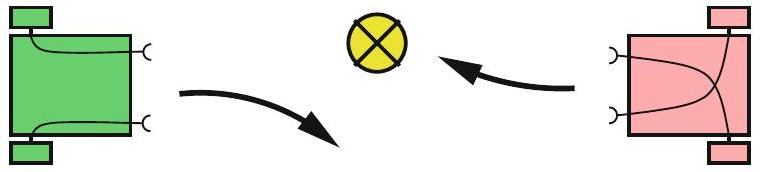
\includegraphics[max width=\textwidth, center]{2025_05_12_af19cd5e0d1b8a465ffeg-009}

Fig. 1.1 Two very simple Braitenberg vehicles and their reactions to a light source\\[0pt]
complex behavior can be produced by very simple electrical circuits [Bra84]. So-called Braitenberg vehicles have two wheels, each of which is driven by an independent electric motor. The speed of each motor is influenced by a light sensor on the front of the vehicle as shown in Fig. 1.1. The more light that hits the sensor, the faster the motor runs. Vehicle 1 in the left part of the figure, according to its configuration, moves away from a point light source. Vehicle 2 on the other hand moves toward the light source. Further small modifications can create other behavior patterns, such that with these very simple vehicles we can realize the impressive behavior described above.

Clearly the above definition is insufficient because AI has the goal of solving difficult practical problems which are surely too demanding for the Braitenberg vehicle. In the Encyclopedia Britannica [Bri91] one finds a Definition that goes like:

\begin{displayquote}
AI is the ability of digital computers or computer controlled robots to solve problems that are normally associated with the higher intellectual processing capabilities of humans ...
\end{displayquote}

But this definition also has weaknesses. It would admit for example that a computer with large memory that can save a long text and retrieve it on demand displays intelligent capabilities, for memorization of long texts can certainly be considered a higher intellectual processing capability of humans, as can for example the quick multiplication of two 20-digit numbers. According to this definition, then, every computer is an AI system. This dilemma is solved elegantly by the following definition by Elaine Rich [Ric83]:

\begin{displayquote}
Artificial Intelligence is the study of how to make computers do things at which, at the moment, people are better.
\end{displayquote}

Rich, tersely and concisely, characterizes what AI researchers have been doing for the last 50 years. Even in the year 2050, this definition will be up to date.

Tasks such as the execution of many computations in a short amount of time are the strong points of digital computers. In this regard they outperform humans by many multiples. In many other areas, however, humans are far superior to machines. For instance, a person entering an unfamiliar room will recognize the surroundings within fractions of a second and, if necessary, just as swiftly make decisions and plan actions. To date, this task is too demanding for autonomous ${ }^{1}$

\footnotetext{${ }^{1}$ An autonomous robot works independently, without manual support, in particular without remote control.
}
robots. According to Rich's definition, this is therefore a task for AI. In fact, research on autonomous robots is an important, current theme in AI. Construction of chess computers, on the other hand, has lost relevance because they already play at or above the level of grandmasters.

It would be dangerous, however, to conclude from Rich's definition that AI is only concerned with the pragmatic implementation of intelligent processes. Intelligent systems, in the sense of Rich's definition, cannot be built without a deep understanding of human reasoning and intelligent action in general, because of which neuroscience (see Sect. 1.1.1) is of great importance to AI. This also shows that the other cited definitions reflect important aspects of AI.

A particular strength of human intelligence is adaptivity. We are capable of adjusting to various environmental conditions and change our behavior accordingly through learning. Precisely because our learning ability is so vastly superior to that of computers, machine learning is, according to Rich's definition, a central subfield of AI.

\subsection*{1.1.1 Brain Science and Problem Solving}
Through research of intelligent systems we can try to understand how the human brain works and then model or simulate it on the computer. Many ideas and principles in the field of neural networks (see Chap. 9) stem from brain science with the related field of neuroscience.

A very different approach results from taking a goal-oriented line of action, starting from a problem and trying to find the most optimal solution. How humans solve the problem is treated as unimportant here. The method, in this approach, is secondary. First and foremost is the optimal intelligent solution to the problem. Rather than employing a fixed method (such as, for example, predicate logic) AI has as its constant goal the creation of intelligent agents for as many different tasks as possible. Because the tasks may be very different, it is unsurprising that the methods currently employed in AI are often also quite different. Similar to medicine, which encompasses many different, often life-saving diagnostic and therapy procedures, AI also offers a broad palette of effective solutions for widely varying applications. For mental inspiration, consider Fig. 1.2 on page 4. Just as in medicine, there is no universal method for all application areas of AI, rather a great number of possible solutions for the great number of various everyday problems, big and small.

Cognitive science is devoted to research into human thinking at a somewhat higher level. Similarly to brain science, this field furnishes practical AI with many important ideas. On the other hand, algorithms and implementations lead to further important conclusions about how human reasoning functions. Thus these three fields benefit from a fruitful interdisciplinary exchange. The subject of this book, however, is primarily problem-oriented AI as a subdiscipline of computer science.

There are many interesting philosophical questions surrounding intelligence and artificial intelligence. We humans have consciousness; that is, we can think about\\
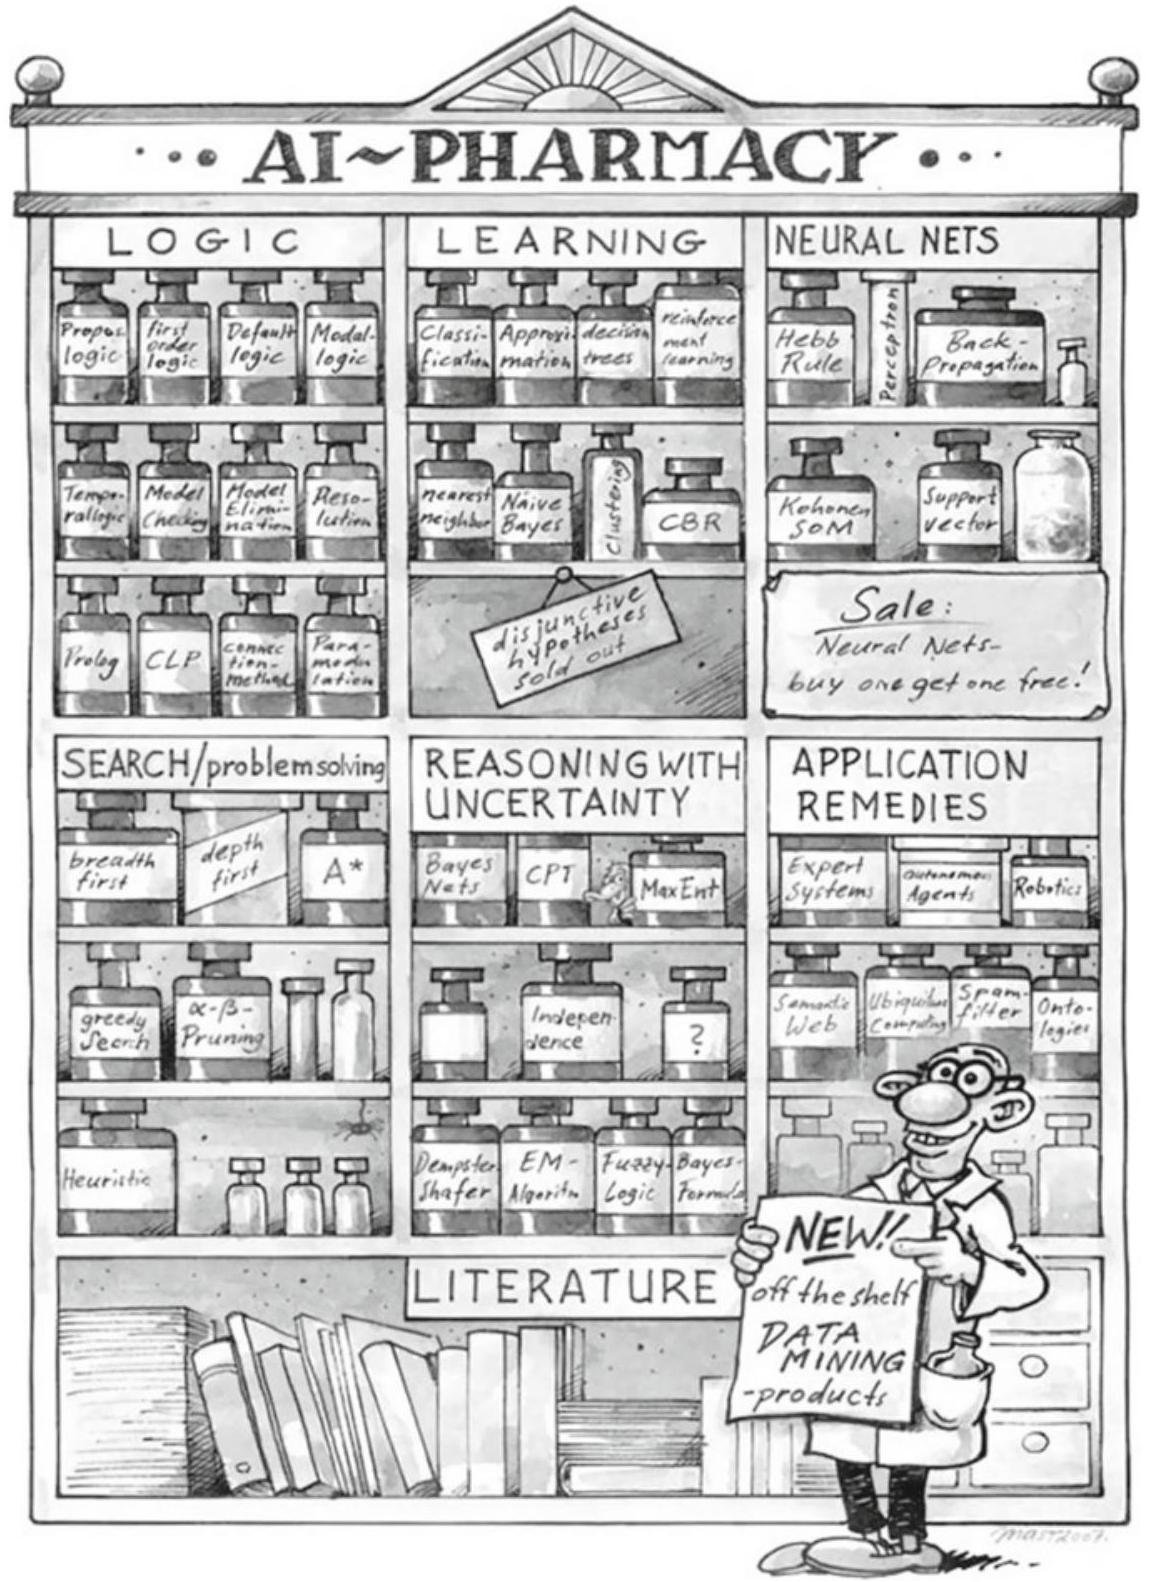
\includegraphics[max width=\textwidth, center]{2025_05_12_af19cd5e0d1b8a465ffeg-011}

Fig. 1.2 A small sample of the solutions offered by AI\\
ourselves and even ponder that we are able to think about ourselves. How does consciousness come to be? Many philosophers and neurologists now believe that the mind and consciousness are linked with matter, that is, with the brain. The\\[0pt]
question of whether machines could one day have a mind or consciousness could at some point in the future become relevant. The mind-body problem in particular concerns whether or not the mind is bound to the body. We will not discuss these questions here. The interested reader may consult [Spe98, Spe97] and is invited, in the course of AI technology studies, to form a personal opinion about these questions.

\subsection*{1.1.2 The Turing Test and Chatterbots}
Alan Turing made a name for himself as an early pioneer of AI with his definition of an intelligent machine, in which the machine in question must pass the following test. The test person Alice sits in a locked room with two computer terminals. One terminal is connected to a machine, the other with a non-malicious person Bob. Alice can type questions into both terminals. She is given the task of deciding, after five minutes, which terminal belongs to the machine. The machine passes the test if it can trick Alice at least $30 \%$ of the time [Tur50].

While the test is very interesting philosophically, for practical AI, which deals with problem solving, it is not a very relevant test. The reasons for this are similar to those mentioned above related to Braitenberg vehicles (see Exercise 1.3 on page 21).

The AI pioneer and social critic Joseph Weizenbaum developed a program named Eliza, which is meant to answer a test subject's questions like a human psychologist [Wei66]. He was in fact able to demonstrate success in many cases. Supposedly his secretary often had long discussions with the program. Today in the internet there are many so-called chatterbots, some of whose initial responses are quite impressive. After a certain amount of time, however, their artificial nature becomes apparent. Some of these programs are actually capable of learning, while others possess extraordinary knowledge of various subjects, for example geography or software development. There are already commercial applications for chatterbots in online customer support and there may be others in the field of e-learning. It is conceivable that the learner and the e-learning system could communicate through a chatterbot. The reader may wish to compare several chatterbots and evaluate their intelligence in Exercise 1.1 on page 20.

\subsection*{1.2 The History of AI}
AI draws upon many past scientific achievements which are not mentioned here, for AI as a science in its own right has only existed since the middle of the Twentieth Century. Table 1.1 on page 6, with the most important AI milestones, and a graphical representation of the main movements of AI in Fig. 1.3 on page 8 complement the following text.

Table 1.1 Milestones in the development of AI from Gödel to today

\begin{center}
\begin{tabular}{|l|l|}
\hline
1931 & The Austrian Kurt Gödel shows that in first-order predicate logic all true statements are derivable [Göd31a]. In higher-order logics, on the other hand, there are true statements that are unprovable [Göd31b]. (In [Göd31b] Gödel showed that predicate logic extended with the axioms of arithmetic is incomplete.) \\
\hline
1937 & Alan Turing points out the limits of intelligent machines with the halting problem [Tur37]. \\
\hline
1943 & McCulloch and Pitts model neural networks and make the connection to propositional logic. \\
\hline
1950 & Alan Turing defines machine intelligence with the Turing test and writes about learning machines and genetic algorithms [Tur50]. \\
\hline
1951 & Marvin Minsky develops a neural network machine. With 3000 vacuum tubes he simulates 40 neurons. \\
\hline
1955 & Arthur Samuel (IBM) builds a learning checkers program that plays better than its developer [Sam59]. \\
\hline
\multirow[t]{2}{*}{1956} & McCarthy organizes a conference in Dartmouth College. Here the name Artificial Intelligence was first introduced. \\
\hline
 & Newell and Simon of Carnegie Mellon University (CMU) present the Logic Theorist, the first symbol-processing computer program [NSS83]. \\
\hline
1958 & McCarthy invents at MIT (Massachusetts Institute of Technology) the high-level language LISP. He writes programs that are capable of modifying themselves. \\
\hline
1959 & Gelernter (IBM) builds the Geometry Theorem Prover. \\
\hline
1961 & The General Problem Solver (GPS) by Newell and Simon imitates human thought [NS61]. \\
\hline
1963 & McCarthy founds the AI Lab at Stanford University. \\
\hline
1965 & Robinson invents the resolution calculus for predicate logic [Rob65] (Sect. 3.5). \\
\hline
1966 & Weizenbaum's program Eliza carries out dialog with people in natural language [Wei66] (Sect. 1.1.2). \\
\hline
1969 & Minsky and Papert show in their book Perceptrons that the perceptron, a very simple neural network, can only represent linear functions [MP69] (Sect. 1.1.2). \\
\hline
\multirow[t]{2}{*}{1972} & French scientist Alain Colmerauer invents the logic programming language PROLOG (Chap. 5). \\
\hline
 & British physician de Dombal develops an expert system for diagnosis of acute abdominal pain [dDLS+72]. It goes unnoticed in the mainstream AI community of the time (Sect. 7.3). \\
\hline
1976 & Shortliffe and Buchanan develop MYCIN, an expert system for diagnosis of infectious diseases, which is capable of dealing with uncertainty (Chap. 7). \\
\hline
1981 & Japan begins, at great expense, the "Fifth Generation Project" with the goal of building a powerful PROLOG machine. \\
\hline
1982 & R1, the expert system for configuring computers, saves Digital Equipment Corporation 40 million dollars per year [McD82]. \\
\hline
1986 & Renaissance of neural networks through, among others, Rumelhart, Hinton and Sejnowski [RM86]. The system Nettalk learns to read texts aloud [SR86] (Chap. 9). \\
\hline
1990 & Pearl [Pea88], Cheeseman [Che85], Whittaker, Spiegelhalter bring probability theory into AI with Bayesian networks (Sect. 7.4). Multi-agent systems become popular. \\
\hline
\end{tabular}
\end{center}

Table 1.1 (continued)

\begin{center}
\begin{tabular}{|l|l|}
\hline
1992 & Tesauros TD-gammon program demonstrates the advantages of reinforcement learning. \\
\hline
1993 & Worldwide RoboCup initiative to build soccer-playing autonomous robots [Roba]. \\
\hline
1995 & From statistical learning theory, Vapnik develops support vector machines, which are very important today. \\
\hline
1997 & IBM's chess computer Deep Blue defeats the chess world champion Gary Kasparov. \\
\hline
 & First international RoboCup competition in Japan. \\
\hline
2003 & The robots in RoboCup demonstrate impressively what AI and robotics are capable of achieving. \\
\hline
2006 & Service robotics becomes a major AI research area. \\
\hline
2009 & First Google self-driving car drives on the California freeway. \\
\hline
2010 & Autonomous robots begin to improve their behavior through learning. \\
\hline
2011 & IBM's "Watson" beats two human champions on the television game show "Jeopardy!". Watson understands natural language and can answer difficult questions very quickly (Sect. 1.4). \\
\hline
\multirow[t]{4}{*}{2015} & Daimler premiers the first autonomous truck on the Autobahn. \\
\hline
 & Google self-driving cars have driven over one million miles and operate within cities. \\
\hline
 & Deep learning (Sect. 11.9) enables very good image classification. \\
\hline
 & Paintings in the style of the Old Masters can be automatically generated with deep learning. AI becomes creative! \\
\hline
2016 & The Go program AlphaGo by Google DeepMind [SHM+16] beats the European champion 5:0 in January and Korean Lee Sedol, one of the world's best Go players, 4:1 in March. Deep learning techniques applied to pattern recognition, as well as reinforcement learning and Monte Carlo tree search lead to this success. \\
\hline
\end{tabular}
\end{center}

\subsection*{1.2.1 The First Beginnings}
In the 1930s Kurt Gödel, Alonso Church, and Alan Turing laid important foundations for logic and theoretical computer science. Of particular interest for AI are Gödel's theorems. The completeness theorem states that first-order predicate logic is complete. This means that every true statement that can be formulated in predicate logic is provable using the rules of a formal calculus. On this basis, automatic theorem provers could later be constructed as implementations of formal calculi. With the incompleteness theorem, Gödel showed that in higher-order logics there exist true statements that are unprovable. ${ }^{2}$ With this he uncovered painful limits of formal systems.

Alan Turing's proof of the undecidability of the halting problem also falls into this time period. He showed that there is no program that can decide whether a given arbitrary program (and its respective input) will run in an infinite loop. With

\footnotetext{${ }^{2}$ Higher-order logics are extensions of predicate logic, in which not only variables, but also function symbols or predicates can appear as terms in a quantification. Indeed, Gödel only showed that any system that is based on predicate logic and can formulate Peano arithmetic is incomplete.
}
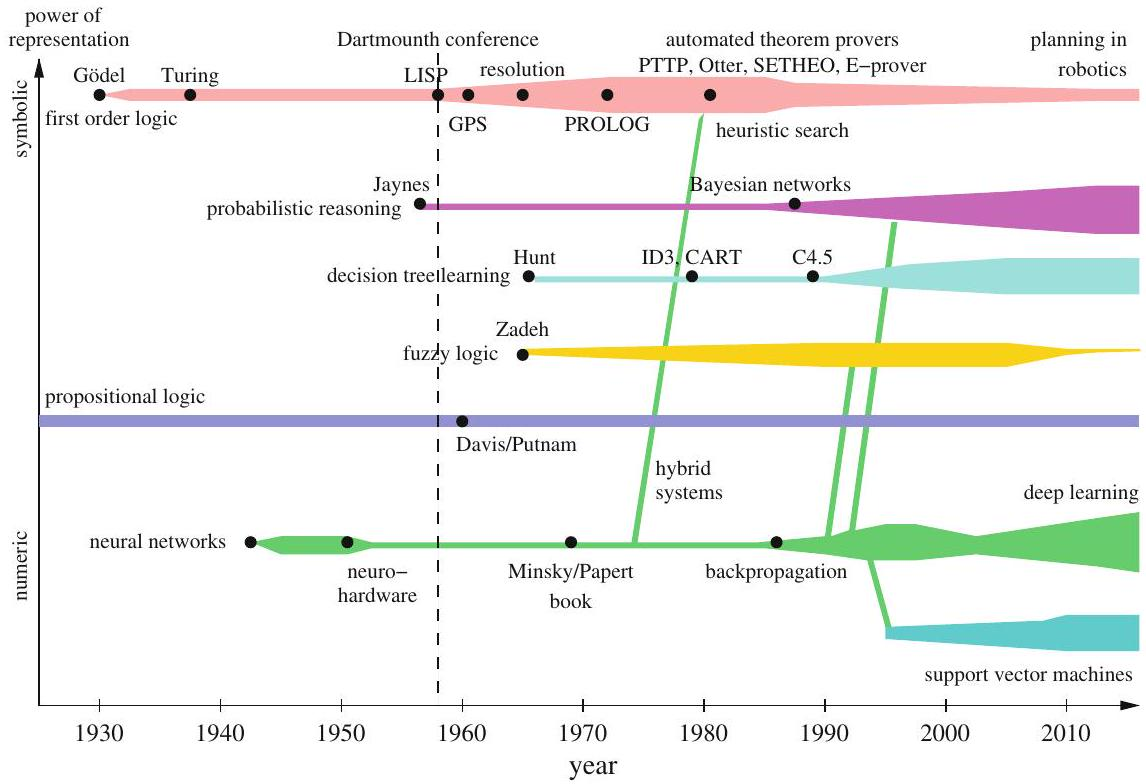
\includegraphics[max width=\textwidth, center]{2025_05_12_af19cd5e0d1b8a465ffeg-015}

Fig. 1.3 History of the various AI areas. The width of the bars indicates prevalence of the method's use\\
this Turing also identified a limit for intelligent programs. It follows, for example, that there will never be a universal program verification system. ${ }^{3}$

In the 1940s, based on results from neuroscience, McCulloch, Pitts and Hebb designed the first mathematical models of neural networks. However, computers at that time lacked sufficient power to simulate simple brains.

\subsection*{1.2.2 Logic Solves (Almost) All Problems}
AI as a practical science of thought mechanization could of course only begin once there were programmable computers. This was the case in the 1950s. Newell and Simon introduced Logic Theorist, the first automatic theorem prover, and thus also showed that with computers, which actually only work with numbers, one can also process symbols. At the same time McCarthy introduced, with the language LISP, a programming language specially created for the processing of symbolic structures. Both of these systems were introduced in 1956 at the historic Dartmouth Conference, which is considered the birthday of AI.

In the US, LISP developed into the most important tool for the implementation of symbol-processing AI systems. Thereafter the logical inference rule known as resolution developed into a complete calculus for predicate logic.

\footnotetext{${ }^{3}$ This statement applies to "total correctness", which implies a proof of correct execution as well as a proof of termination for every valid input.
}In the 1970s the logic programming language PROLOG was introduced as the European counterpart to LISP. PROLOG offers the advantage of allowing direct programming using Horn clauses, a subset of predicate logic. Like LISP, PROLOG has data types for convenient processing of lists.

Until well into the 1980s, a breakthrough spirit dominated AI, especially among many logicians. The reason for this was the string of impressive achievements in symbol processing. With the Fifth Generation Computer Systems project in Japan and the ESPRIT program in Europe, heavy investment went into the construction of intelligent computers.

For small problems, automatic provers and other symbol-processing systems sometimes worked very well. The combinatorial explosion of the search space, however, defined a very narrow window for these successes. This phase of AI was described in [RN10] as the "Look, Ma, no hands!" era.

Because the economic success of AI systems fell short of expectations, funding for logic-based AI research in the United States fell dramatically during the 1980s.

\subsection*{1.2.3 The New Connectionism}
During this phase of disillusionment, computer scientists, physicists, and Cognitive scientists were able to show, using computers which were now sufficiently powerful, that mathematically modeled neural networks are capable of learning using training examples, to perform tasks which previously required costly programming. Because of the fault-tolerance of such systems and their ability to recognize patterns, considerable successes became possible, especially in pattern recognition. Facial recognition in photos and handwriting recognition are two example applications. The system Nettalk was able to learn speech from example texts [SR86]. Under the name connectionism, a new subdiscipline of AI was born.

Connectionism boomed and the subsidies flowed. But soon even here feasibility limits became obvious. The neural networks could acquire impressive capabilities, but it was usually not possible to capture the learned concept in simple formulas or logical rules. Attempts to combine neural nets with logical rules or the knowledge of human experts met with great difficulties. Additionally, no satisfactory solution to the structuring and modularization of the networks was found.

\subsection*{1.2.4 Reasoning Under Uncertainty}
AI as a practical, goal-driven science searched for a way out of this crisis. One wished to unite logic's ability to explicitly represent knowledge with neural networks' strength in handling uncertainty. Several alternatives were suggested.

The most promising, probabilistic reasoning, works with conditional probabilities for propositional calculus formulas. Since then many diagnostic and expert systems have been built for problems of everyday reasoning using Bayesian\\
networks. The success of Bayesian networks stems from their intuitive comprehensibility, the clean semantics of conditional probability, and from the centuries-old, mathematically grounded probability theory.

The weaknesses of logic, which can only work with two truth values, can be solved by fuzzy logic, which pragmatically introduces infinitely many values between zero and one. Though even today its theoretical foundation is not totally firm, it is being successfully utilized, especially in control engineering.

A much different path led to the successful synthesis of logic and neural networks under the name hybrid systems. For example, neural networks were employed to learn heuristics for reduction of the huge combinatorial search space in proof discovery [SE90].

Methods of decision tree learning from data also work with probabilities. Systems like CART, ID3 and C4.5 can quickly and automatically build very accurate decision trees which can represent propositional logic concepts and then be used as expert systems. Today they are a favorite among machine learning techniques (Sect. 8.4).

Since about 1990, data mining has developed as a subdiscipline of AI in the area of statistical data analysis for extraction of knowledge from large databases. Data mining brings no new techniques to AI, rather it introduces the requirement of using large databases to gain explicit knowledge. One application with great market potential is steering ad campaigns of big businesses based on analysis of many millions of purchases by their customers. Typically, machine learning techniques such as decision tree learning come into play here.

\subsection*{1.2.5 Distributed, Autonomous and Learning Agents}
Distributed artificial intelligence, DAI, has been an active area research since about 1985. One of its goals is the use of parallel computers to increase the efficiency of problem solvers. It turned out, however, that because of the high computational complexity of most problems, the use of "intelligent" systems is more beneficial than parallelization itself.

A very different conceptual approach results from the development of autonomous software agents and robots that are meant to cooperate like human teams. As with the aforementioned Braitenberg vehicles, there are many cases in which an individual agent is not capable of solving a problem, even with unlimited resources. Only the cooperation of many agents leads to the intelligent behavior or to the solution of a problem. An ant colony or a termite colony is capable of erecting buildings of very high architectural complexity, despite the fact that no single ant comprehends how the whole thing fits together. This is similar to the situation of provisioning bread for a large city like New York [RN10]. There is no central planning agency for bread, rather there are hundreds of bakers that know their respective areas of the city and bake the appropriate amount of bread at those locations.

Active skill acquisition by robots is an exciting area of current research. There are robots today, for example, that independently learn to walk or to perform\\
various motorskills related to soccer (Chap. 10). Cooperative learning of multiple robots to solve problems together is still in its infancy.

\subsection*{1.2.6 Al Grows Up}
The above systems offered by AI today are not a universal recipe, but a workshop with a manageable number of tools for very different tasks. Most of these tools are well-developed and are available as finished software libraries, often with convenient user interfaces. The selection of the right tool and its sensible use in each individual case is left to the AI developer or knowledge engineer. Like any other artisanship, this requires a solid education, which this book is meant to promote.

More than nearly any other science, AI is interdisciplinary, for it draws upon interesting discoveries from such diverse fields as logic, operations research, statistics, control engineering, image processing, linguistics, philosophy, psychology, and neurobiology. On top of that, there is the subject area of the particular application. To successfully develop an AI project is therefore not always so simple, but almost always extremely exciting.

\subsection*{1.2.7 The Al Revolution}
Around the year 2010 after about 25 years of research on neural networks, scientists could start harvesting the fruits of their research. The very powerful deep learning networks can for example learn to classify images with very high arruracy. Since image classification is of crucial importance for all types of smart robots, this initiated the AI revolution which in turn leads to smart self-driving cars and service robots.

\subsection*{1.3 AI and Society}
There have been many scientific books and science fiction novels written on all aspects of this subject. Due to great advances in AI research, we have been on the brink of the age of autonomous robots and the Internet of Things since roughly 2005. Thus we are increasingly confronted with AI in everyday life. The reader, who may soon be working as an AI developer, must also deal with the social impact of this work. As an author of a book on AI techniques, I have the crucial task of examining this topic. I would like to deal with some particularly important aspects of AI which are of great practical relevance for our lives.

\subsection*{1.3.1 Does Al Destroy Jobs?}
In January 2016, the World Econonic Forum published a study [SS16], frequently cited by the German press, predicting that "industry 4.0 " would destroy over five\\
million jobs in the next five years. This forecast is hardly surprising because automation in factories, offices, administration, transportation, in the home and in many other areas has led to continually more work being done by computers, machines and robots. AI has been one of the most important factors in this trend since about 2010.

Presumably, the majority of people would gladly leave physically hard, dirty and unhealthy jobs and tasks to machines. Thus automation is a complete blessing for humanity, assuming it does not result in negative side effects, such as harm to the environment. Many of the aforementioned unpleasant jobs can be done faster, more precisely, and above all cheaper by machines. This seems almost like a trend towards paradise on Earth, where human beings do less and less unpleasant work and have correspondingly more time for the good things in life. This seems almost like a trend towards paradise on earth. We have to do less and less unpleasant work and in turn have more time for the good things in life. ${ }^{4}$ All the while, we would enjoy the same (or potentially even increasing) prosperity, for the economy would not employ these machines if they did not markedly raise productivity.

Unfortunately we are not on the road to paradise. For several decades, we have worked more than 40 hours per week, have been stressed, complained of burnout and other sicknesses, and suffered a decline in real wages. How can this be, if productivity is continually increasing? Many economists say that the reason for this is competitive pressure. In an effort to compete and deliver the lowest priced goods to market, companies need to lower production costs and thus lay off workers. This results in the aforementioned unemployment. In order to avoid a drop in sales volume due to reduced prices, more products need to be manufactured and sold. The economy must grow!

If the economy continues to grow in a country in which the population is no longer growing (as is the case in most modern industrialized countries), each citizen must necessarily consume more. For that to happen, new markets must be created, ${ }^{5}$ and marketing has the task of convincing us that we want the new products. This is-allegedly-the only way to "sustainably" ensure prosperity. Apparently there seems to be no escape from this growth/consumption spiral. This has two fatal consequences. For one thing, this increase in consumption should make people happier, but it is having quite the opposite effect: mental illness is increasing.

Even more obvious and, above all, fatal, are economic growth's effects on our living conditions. It is no secret that the earth's growth limit has long been exceeded [MMZM72, Ran12], and that we are overexploiting nature's nonrenewable resources. We are therefore living at the expense of our children and grandchildren, who consequently will have poorer living conditions than we have today. It is also known that every additional dollar of economic growth is an additional burden on the environment-for example through additional $\mathrm{CO}_{2}$ concentration in the atmosphere and the resulting climate change [Pae16]. We are destroying our own basis of

\footnotetext{${ }^{4}$ Those of us, such as scientists, computer scientists and engineers, who enjoy it may of course continue our work.\\
${ }^{5}$ Many EU and German Ministry of Education and Research funding programs for example require that scientists who submit proposals show evidence that their research will open up new markets.
}
existence. Thus it is obvious that we should abandon this path of growth for the sake of a livable future. But how?

Let's think back to the road to paradise that AI is supposedly preparing for us. Apparently, as we practice it, it does not lead to paradise. Understanding this problem and finding the right path is one of the central tasks of today. Because of inherent complexities, this problem can not be fully dealt with in an introductory AI textbook. However, I would like to provide the reader with a little food for thought.

Although productivity is growing steadily in almost all areas of the economy, workers are required to work as hard as ever. They do not benefit from the increase in productivity. So, we must ask, where do the profits go? Evidently not to the people to whom they are owed, i.e. the workers. Instead, part of the profits is spent on investment and thus on further growth and the rest is taken by the capital owners, while employees work the same hours for declining real wages [Pik14]. This leads to ever-increasing capital concentration among a few rich individuals and private banks, while on the other hand increasing poverty around the world is creating political tensions that result in war, expulsion and flight.

What is missing is a fair and just distribution of profits. How can this be achieved? Politicians and economists are continually trying to optimize our economic system, but politics has not offered a sustainable solution, and too few economists are investigating this highly exciting economic question. Obviously the attempt to optimize the parameters of our current capitalist economic system has not lead to a more equitable distribution of wealth, but to the opposite.

This is why economists and financial scientists must begin to question the system and look for alternatives. We should ask ourselves how to change the rules and laws of the economy so that all people profit from increased productivity. A growing community of economists and sustainability scientists have offered interesting solutions, a few of which I will briefly describe here.

Problem Number One is the creation of fiat money by the banks. New moneywhich is needed, among other things, to keep our growing economy going-is now being created by private banks. This is made possible by the fact that banks have to own only a small part, namely the minimum cash reserve ratio, of the money they give as loans. In the EU in 2016, the minimum cash reserve ratio is one percent.

States then borrow this money from private banks in the form of government bonds and thus fall into debt. This is how our current government debt crises have developed. This problem can be solved easily by prohibiting creation of money by the banks by increasing the minimum cash reserve ratio to $100 \%$. State central banks will then get back the monopoly on creating money, and the newly created money can be used directly by the state for the purposes of social welfare. It should be evident that this simple measure would significantly ease the problem of public debt.

Further interesting components of such an economic reform could be the conversion of the current interest rate system to the so-called natural economic order [GP58], and the introduction of the "economy for the common good" [Fel14] and the biophysical economy [GK09, Küm11]. The practical implementation of the economy for the common good would involve a tax reform, the most important elements of which would be the abolition of the income tax and substantially increased value\\
added tax on energy and resource consumption. We would thus arrive at a highly prosperous, more sustainable human world with less environmental damage and more local trade. The reader may study the literature and assess whether the ideas quoted here are interesting and, if necessary, help to make the required changes.

To conclude this section, I would like to quote the famous physicist Stephen Hawking. In a community-driven interview on \href{http://www.reddit.com}{www.reddit.com} he gave the following answer to whether he had any thoughts about unemployment caused by automation:

\begin{displayquote}
If machines produce everything we need, the outcome will depend on how things are distributed. Everyone can enjoy a life of luxurious leisure if the machine-produced wealth is shared, or most people can end up miserably poor if the machine-owners successfully lobby against wealth redistribution. So far, the trend seems to be toward the second option, with technology driving ever-increasing inequality.
\end{displayquote}

Another Hawking quotation is also fitting. During the same interview, ${ }^{6}$ to an AI professor's question about which moral ideas he should impart to his students, Hawking answered:

\begin{displayquote}
... Please encourage your students to think not only about how to create AI, but also about how to ensure its beneficial use.
\end{displayquote}

As a consequence we should question the reasonableness of AI applications such as the export of intelligent cruise missiles to "allied" Arab states, the deployment of humanoid combat robots, etc.

\subsection*{1.3.2 Al and Transportation}
In the past 130 years, automotive industry engineers have made great strides. In Germany, one out of every two people owns their own car. These cars are highly reliable. This makes us very mobile and we use this very convenient mobility in work, everyday life and leisure. Moreover, we are dependent on it. Today, we can not get by without a motor vehicle, especially in rural areas with weak public transportation infrastructure, as for instance in Upper Swabia, where the author and his students live.

The next stage of increased convenience in road transportation is now imminent. In a few years, we will be able to buy electric self-driving cars, i.e. robotic cars, which will autonomously bring us to almost any destination. All passengers in the robotic car would be able to read, work or sleep during the trip. This is possible on public transit already, but passengers in a robotic car would be able to do this at any time and on any route.

Autonomous vehicles that can operate independently could also travel without passengers. This will lead to yet another increase in convenience: robotic taxis. Via a smartphone app, we will be able to order the optimal taxi, in terms of size and equipment, for any conceivable transportation purpose. We will be able to choose whether we want to travel alone in the taxi or whether we are willing to share a ride with

\footnotetext{${ }^{6}$ \href{https://www.reddit.com/user/Prof-Stephen-Hawking}{https://www.reddit.com/user/Prof-Stephen-Hawking}.
}
other passengers. We will not need our own car anymore. All associated responsibilities and expenses, such as refueling, technical service, cleaning, searching for parking, buying and selling, garage rent, etc. are void, which saves us money and effort.

Besides the immediate gains in comfort and convenience, robotic cars will offer other significant advantages. For example, according to a McKinsey study [GHZ14], we will need far fewer cars and, above all, far fewer parking places in the era of self-driving cars, which will lead to an immense reduction in resource consumption. According to a Lawrence Berkeley National Laboratory study [GS15], electric self-driving cars will cause a $90 \%$ reduction in green house emissions per passenger mile due to the vehicles' energy efficiency and the optimized fit between the vehicle and its purpose. Due to their optimal resource utilization, robotic taxis will be much more environmentally friendly than, for example, heavy buses, which often run at low capacity, especially in rural areas. Overall, robot taxis will contribute dramatically to energy savings and thus, among other things, to a significant improvement in $\mathrm{CO}_{2}$ and climate problems.

Passenger safety will be much higher than it is today. Experts currently estimate future accident rates between zero and ten percent compared to today. Emotional driving ("road rage"), distracted driving and driving under the influence of drugs and alcohol will no longer exist.

Taxi drivers losing their jobs is often cited as a disadvantage of robotic cars. It is almost certain that there will no longer be taxi drivers from about 2030 onwards, but that is not necessarily a problem. As explained in the previous section, our society just needs to deal with the newly gained productivity properly.

In addition to the many advantages mentioned above, robotic cars have two critical problems. Firstly, the so-called rebound effect will nullify at least some of the gains in resource, energy and time savings. Shorter driving times as well as more comfortable and cheaper driving will tempt us to drive more. We can only deal with this problem by rethinking our attitude towards consumption and quality of life. Do we have to use the entire time saved for more activities? Here we are all invited to critical reflection.

Another problem we should take seriously is that the robotic cars will need to be networked. In principle, this gives hackers and terrorists the ability to access and manipulate the vehicles' controls through security holes in their network protocols. If a hacker manages to do this once, he could repeat the attack on a grand scale, potentially bringing entire vehicle fleets to a halt, causing accidents, spying on vehicle occupants, or initiating other criminal actions. Here, as in other areas such as home automation and the Internet of Things, IT security experts will be needed to ensure the highest possible security guarantees using tools of the trade such as cryptographic methods. By the way, improved machine learning algorithms will be useful in detecting hacking attacks.

\subsection*{1.3.3 Service Robotics}
In a few years, shortly after self-driving cars, the next bit of consumption bait on the shelves of electronics stores will be service robots. Recently the Google subsidiary

Fig. 1.4 The assistance robot Marvin, deployed in the AsRoBe research project\\
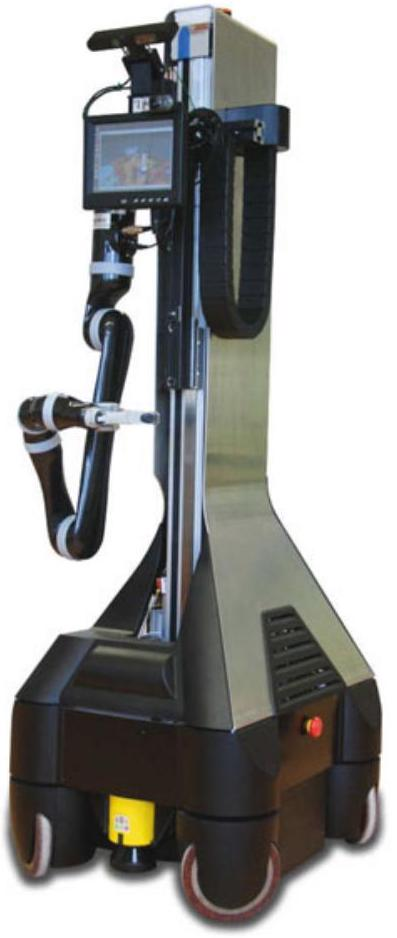
\includegraphics[max width=\textwidth, center]{2025_05_12_af19cd5e0d1b8a465ffeg-023}

Boston Dynamics provided an impressive example in its humanoid robot Atlas. ${ }^{7}$ Like the new cars, service robots offer a large gain in comfort and convenience which we would probably like to enjoy. One need only imagine such a robot dutifully cleaning and scrubbing after a party from night until morning without a grumble. Or think of the help that an assistance robot like Marvin, shown in Fig. 1.4, could provide to the elderly ${ }^{8}$ or to people with disabilities [SPR+16].

In contrast to the robotic cars, however, these benefits come with costlier trade-offs. Completely new markets would be created, more natural resources and more energy would be consumed, and it is not even certain that people's lives would be simplified by the use of service robots in all areas. One of the first applications for robots like Atlas, developed by Boston Dynamics in contract with Google, will probably be military combat.

It is therefore all the more important that, before these robots come to market, we engage in social discourse on this topic. Science fiction films, such as "Ex Machina" (2015) with its female androids, the chilling "I, Robot" (2004) or the humorous "Robot and Frank" (2012), which depicts the pleasant side of a service robot as an old man's helper, can also contribute to such a discussion.

\footnotetext{${ }^{7}$ \href{https://youtu.be/rVlhMGQgDkY}{https://youtu.be/rVlhMGQgDkY}.\\
${ }^{8}$ In the coming demographic shift, assistance robots could become important for the elderly and thus for our whole society.
}\subsection*{1.4 Agents}
Although the term intelligent agents is not new to AI, only in recent years has it gained prominence through [RN10], among others. Agent denotes rather generally a system that processes information and produces an output from an input. These agents may be classified in many different ways.

In classical computer science, software agents are primarily employed (Fig. 1.5). In this case the agent consists of a program that calculates a result from user input.

In robotics, on the other hand, hardware agents (also called autonomous robots) are employed, which additionally have sensors and actuators at their disposal (Fig. 1.6). The agent can perceive its environment with the sensors. With the actuators it carries out actions and changes its environment.

With respect to the intelligence of the agent, there is a distinction between reflex agents, which only react to input, and agents with memory, which can also include the past in their decisions. For example, a driving robot that through its sensors knows its exact position (and the time) has no way, as a reflex agent, of determining its velocity. If, however, it saves the position, at short, discrete time steps, it can thus easily calculate its average velocity in the previous time interval.

If a reflex agent is controlled by a deterministic program, it represents a function of the set of all inputs to the set of all outputs. An agent with memory, on the other hand, is in general not a function. Why? (See Exercise 1.5 on page 21.) Reflex agents are sufficient in cases where the problem to be solved involves a Markov decision process. This is a process in which only the current state is needed to determine the optimal next action (see Chap. 10).

A mobile robot which should move from room 112 to room 179 in a building takes actions different from those of a robot that should move to room 105. In other words, the actions depend on the goal. Such agents are called goal-based.

Fig. 1.5 A software agent with user interaction\\
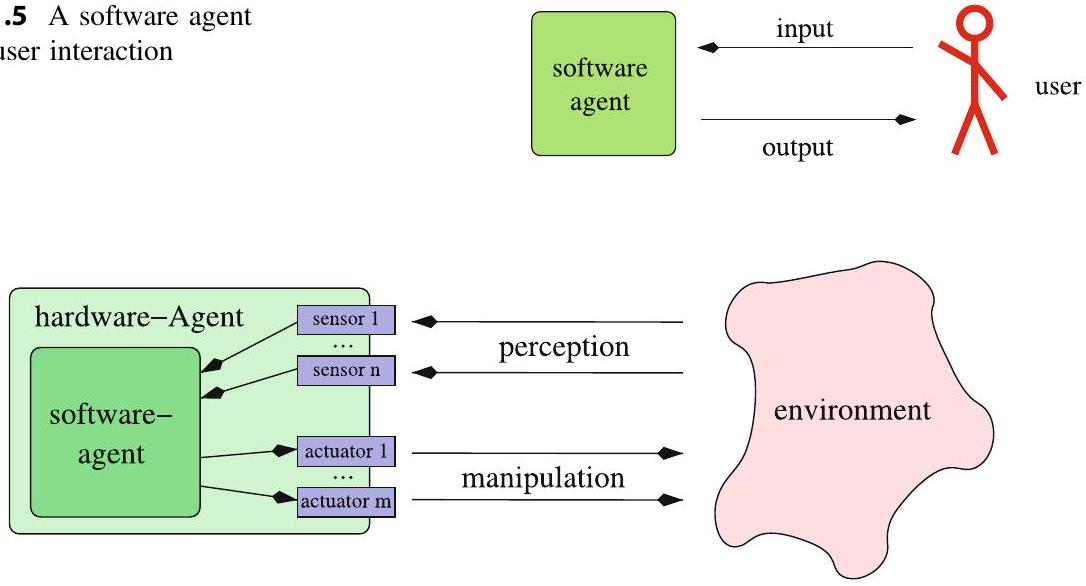
\includegraphics[max width=\textwidth, center]{2025_05_12_af19cd5e0d1b8a465ffeg-024}

Fig. 1.6 A hardware agent

Example 1.1 A spam filter is an agent that puts incoming emails into wanted or unwanted (spam) categories, and deletes any unwanted emails. Its goal as a goalbased agent is to put all emails in the right category. In the course of this not-so-simple task, the agent can occasionally make mistakes. Because its goal is to classify all emails correctly, it will attempt to make as few errors as possible. However, that is not always what the user has in mind. Let us compare the following two agents. Out of 1,000 emails, Agent 1 makes only 12 errors. Agent 2 on the other hand makes 38 errors with the same 1,000 emails. Is it therefore worse than Agent 1? The errors of both agents are shown in more detail in the following table, the so-called "confusion matrix":

\begin{center}
\begin{tabular}{|l|l|l|l|l|l|l|l|}
\hline
\multicolumn{4}{|c|}{Agent 1:} & \multicolumn{4}{|c|}{Agent 2:} \\
\hline
\multicolumn{2}{|c|}{\multirow{2}{*}{}} & \multicolumn{2}{|c|}{correct class} & \multicolumn{2}{|c|}{\multirow{2}{*}{}} & \multicolumn{2}{|c|}{correct class} \\
\hline
 &  & wanted & spam &  &  & wanted & spam \\
\hline
\multirow{2}{*}{spam filter decides} & wanted & 189 & 1 & \multirow{2}{*}{spam filter decides} & wanted & 200 & 38 \\
\hline
 & spam & 11 & 799 &  & spam & 0 & 762 \\
\hline
\end{tabular}
\end{center}

Agent 1 in fact makes fewer errors than Agent 2, but those few errors are severe because the user loses 11 potentially important emails. Because there are in this case two types of errors of differing severity, each error should be weighted with the appropriate cost factor (see Sect. 7.3.5 and Exercise 1.7 on page 21).

The sum of all weighted errors gives the total cost caused by erroneous decisions. The goal of a cost-based agent is to minimize the cost of erroneous decisions in the long term, that is, on average. In Sect. 7.3 we will become familiar with the medical diagnosis system LEXMED as an example of a cost-based agent.

Analogously, the goal of a utility-based agent is to maximize the utility derived from correct decisions in the long term, that is, on average. The sum of all decisions weighted by their respective utility factors gives the total utility.

Of particular interest in AI are Learning agents, which are capable of changing themselves given training examples or through positive or negative feedback, such that the average utility of their actions grows over time (see Chap. 8).

As mentioned in Sect. 1.2.5, distributed agents are increasingly coming into use, whose intelligence are not localized in one agent, but rather can only be seen through cooperation of many agents.

The design of an agent is oriented, along with its objective, strongly toward its environment, or alternately its picture of the environment, which strongly depends on it sensors. The environment is observable if the agent always knows the complete state of the world. Otherwise the environment is only partially observable. If an action always leads to the same result, then the environment is deterministic. Otherwise it is nondeterministic. In a discrete environment only finitely many states and actions occur, whereas a continuous environment boasts infinitely many states or actions.

\subsection*{1.5 Knowledge-Based Systems}
An agent is a program that implements a mapping from perceptions to actions. For simple agents this way of looking at the problem is sufficient. For complex applications in which the agent must be able to rely on a large amount of information and is meant to do a difficult task, programming the agent can be very costly and unclear how to proceed. Here AI provides a clear path to follow that will greatly simplify the work.

First we separate knowledge from the system or program, which uses the knowledge to, for example, reach conclusions, answer queries, or come up with a plan. This system is called the inference mechanism. The knowledge is stored in a knowledge base (KB). Acquisition of knowledge in the knowledge base is denoted Knowledge Engineering and is based on various knowledge sources such as human experts, the knowledge engineer, and databases. Active learning systems can also acquire knowledge through active exploration of the world (see Chap. 10). In Fig. 1.7 the general architecture of knowledge-based systems is presented.

Moving toward a separation of knowledge and inference has several crucial advantages. The separation of knowledge and inference can allow inference systems to be implemented in a largely application-independent way. For example, application of a medical expert system to other diseases is much easier by replacing the knowledge base rather than by programming a whole new system.

Through the decoupling of the knowledge base from inference, knowledge can be stored declaratively. In the knowledge base there is only a description of the knowledge, which is independent from the inference system in use. Without this clear separation, knowledge and processing of inference steps would be interwoven, and any changes to the knowledge would be very costly.\\
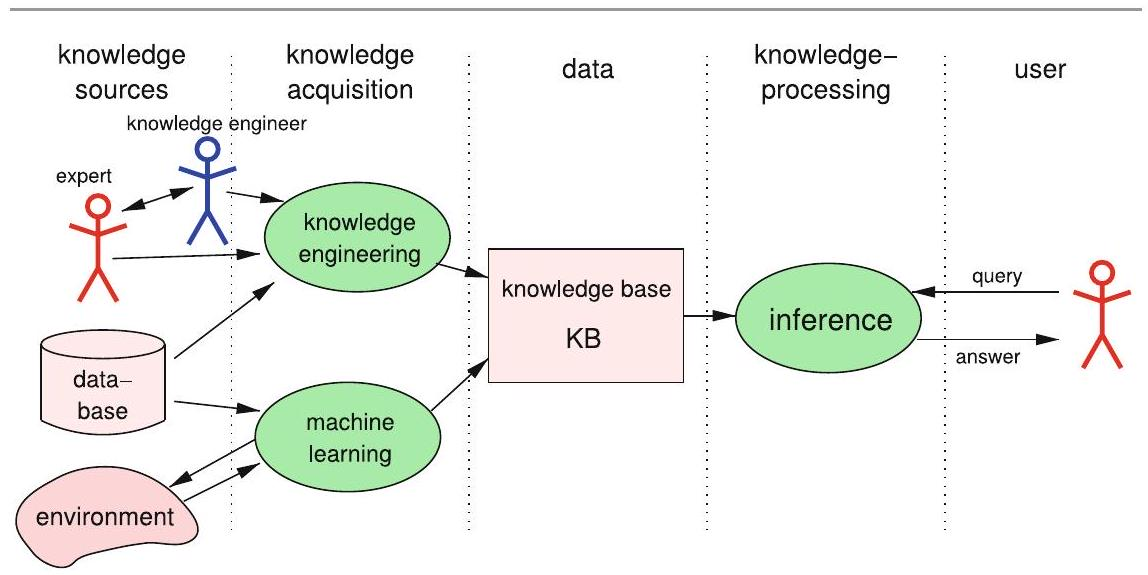
\includegraphics[max width=\textwidth, center]{2025_05_12_af19cd5e0d1b8a465ffeg-026}

Fig. 1.7 Structure of a classic knowledge-processing system

Formal language as a convenient interface between man and machine lends itself to the representation of knowledge in the knowledge base. In the following chapters we will get to know a whole series of such languages. First, in Chaps. 2 and 3 there are propositional calculus and first-order predicate logic (PL1). But other formalisms such as probabilistic logic and decision trees are also presented. We start with propositional calculus and the related inference systems. Building on that, we will present predicate logic, a powerful language that is accessible by machines and very important in AI.

As an example for a large scale knowledge based system we want to refer to the software agent "Watson". Developed at IBM together with a number of universities, Watson is a question answering program, that can be fed with clues given in natural language. It works on a knowledge base comprising four terabytes of hard disk storage, including the full text of Wikipedia [FNA+09]. Watson was developed within IBM's DeepQA project which is characterized in [Dee11] as follows:

\begin{displayquote}
The DeepQA project at IBM shapes a grand challenge in Computer Science that aims to illustrate how the wide and growing accessibility of natural language content and the integration and advancement of Natural Language Processing, Information Retrieval, Machine Learning, Knowledge Representation and Reasoning, and massively parallel computation can drive open-domain automatic Question Answering technology to a point where it clearly and consistently rivals the best human performance.
\end{displayquote}

In the U.S. television quiz show "Jeopardy!", in February 2011, Watson defeated the two human champions Brad Rutter and Ken Jennings in a two-game, combined-point match and won the one million dollar price. One of Watson's particular strengths was its very fast reaction to the questions with the result that Watson often hit the buzzer (using a solenoid) faster than its human competitors and then was able to give the first answer to the question.

The high performance and short reaction times of Watson were due to an implementation on 90 IBM Power 750 servers, each of which contains 32 processors, resulting in 2880 parallel processors.

\subsection*{1.6 Exercises}
Exercise 1.1 Test some of the chatterbots available on the internet. Start for example with \href{http://www.hs-weingarten.de/}{www.hs-weingarten.de/} \~{} ertel/aibook in the collection of links under Turingtest/Chatterbots, or at \href{http://www.simonlaven.com}{www.simonlaven.com} or \href{http://www.alicebot.org}{www.alicebot.org}. Write down a starting question and measure the time it takes, for each of the various programs, until you know for certain that it is not a human.

薬菜 Exercise 1.2 At \href{http://www.pandorabots.com}{www.pandorabots.com} you will find a server on which you can build a chatterbot with the markup language AIML quite easily. Depending on your interest level, develop a simple or complex chatterbot, or change an existing one.

Exercise 1.3 Give reasons for the unsuitability of the Turing test as a definition of "artificial intelligence" in practical AI.\\
\#> Exercise 1.4 Many well-known inference processes, learning processes, etc. are NP-complete or even undecidable. What does this mean for AI?

\section*{Exercise 1.5}
(a) Why is a deterministic agent with memory not a function from the set of all inputs to the set of all outputs, in the mathematical sense?\\
(b) How can one change the agent with memory, or model it, such that it becomes equivalent to a function but does not lose its memory?\\
Exercise 1.6 Let there be an agent with memory that can move within a plane. From its sensors, it receives at clock ticks of a regular interval $\Delta t$ its exact position $(x, y)$ in Cartesian coordinates.\\
(a) Give a formula with which the agent can calculate its velocity from the current time $t$ and the previous measurement of $t-\Delta t$.\\
(b) How must the agent be changed so that it can also calculate its acceleration? Provide a formula here as well.

\section*{薔 Exercise 1.7}
(a) Determine for both agents in Example 1.1 on page 18 the costs created by the errors and compare the results. Assume here that having to manually delete a spam email costs one cent and retrieving a deleted email, or the loss of an email, costs one dollar.\\
(b) Determine for both agents the profit created by correct classifications and compare the results. Assume that for every desired email recognized, a profit of one dollar accrues and for every correctly deleted spam email, a profit of one cent.

\section*{Propositional Logic}
In propositional logic, as the name suggests, propositions are connected by logical operators. The statement "the street is wet" is a proposition, as is "it is raining". These two propositions can be connected to form the new proposition\\
if it is raining the street is wet.\\
Written more formally\\
it is raining $\Rightarrow$ the street is wet.\\
This notation has the advantage that the elemental propositions appear again in unaltered form. So that we can work with propositional logic precisely, we will begin with a definition of the set of all propositional logic formulas.

\subsection*{2.1 Syntax}
Definition 2.1 Let $O p=\{\neg, \wedge, \vee, \Rightarrow, \Leftrightarrow,()$,$\} be the set of logical operators$ and $\Sigma$ a set of symbols. The sets $O p, \Sigma$ and $\{t, f\}$ are pairwise disjoint. $\Sigma$ is called the signature and its elements are the proposition variables. The set of propositional logic formulas is now recursively defined:

\begin{itemize}
  \item $t$ and $f$ are (atomic) formulas.
  \item All proposition variables, that is all elements from $\Sigma$, are (atomic) formulas.
  \item If $A$ and $B$ are formulas, then $\neg A,(A), A \wedge B, A \vee B, A \Rightarrow B, A \Leftrightarrow B$ are also formulas.
\end{itemize}

This elegant recursive definition of the set of all formulas allows us to generate infinitely many formulas. For example, given $\Sigma=\{A, B, C\}$,

$$
A \wedge B, \quad A \wedge B \wedge C, \quad A \wedge A \wedge A, \quad C \wedge B \vee A, \quad(\neg A \wedge B) \Rightarrow(\neg C \vee A)
$$

are formulas. (((A)) $\vee B$ ) is also a syntactically correct formula.

Definition 2.2 We read the symbols and operators in the following way:

$$
\begin{array}{rlrl}
t & : & \text { "true" } & \\
& f: & \text { "false" } & \\
& \neg A: & \text { "not } A \text { " } & \\
A \wedge B: & \text { (negation) } \\
A \vee B: & \text { " } A \text { and } B \text { " } & & \text { (conjunction) } \\
A \Rightarrow B: & & & \text { (disjunction) } \\
A & \Rightarrow B: & \text { "if } A \text { then } B " & \\
A & \text { (implication (also called } \text { material implication) }
\end{array}
$$

The formulas defined in this way are so far purely syntactic constructions without meaning. We are still missing the semantics.

\subsection*{2.2 Semantics}
In propositional logic there are two truth values: $t$ for "true" and $f$ for "false". We begin with an example and ask ourselves whether the formula $A \wedge B$ is true. The answer is: it depends on whether the variables $A$ and $B$ are true. For example, if $A$ stands for "It is raining today" and $B$ for "It is cold today" and these are both true, then $A \wedge B$ is true. If, however, $B$ represents "It is hot today" (and this is false), then $A \wedge B$ is false.

We must obviously assign truth values that reflect the state of the world to proposition variables. Therefore we define

\begin{displayquote}
Definition 2.3 A mapping $I: \Sigma \rightarrow\{t, f\}$, which assigns a truth value to every proposition variable, is called an interpretation.
\end{displayquote}

Because every proposition variable can take on two truth values, every propositional logic formula with $n$ different variables has $2^{n}$ different interpretations. We define the truth values for the basic operations by showing all possible interpretations in a truth table (see Table 2.1 on page 25).

Table 2.1 Definition of the logical operators by truth table

\begin{center}
\begin{tabular}{llllllll}
\hline
$A$ & $B$ & $(A)$ & $\neg A$ & $A \wedge B A \vee B$ & $A \Rightarrow B$ & $A \Leftrightarrow B$ &  \\
\hline
$t$ & $t$ & $t$ & $f$ & $t$ & $t$ & $t$ & $t$ \\
\hline
$t$ & $f$ & $t$ & $f$ & $f$ & $t$ & $f$ & $f$ \\
\hline
$f$ & $t$ & $f$ & $t$ & $f$ & $t$ & $t$ & $f$ \\
\hline
$f$ & $f$ & $f$ & $t$ & $f$ & $f$ & $t$ & $t$ \\
\hline
\end{tabular}
\end{center}

The empty formula is true for all interpretations. In order to determine the truth value for complex formulas, we must also define the order of operations for logical operators. If expressions are parenthesized, the term in the parentheses is evaluated first. For unparenthesized formulas, the priorities are ordered as follows, beginning with the strongest binding: $\neg, \wedge, \vee, \Rightarrow, \Leftrightarrow$.

To clearly differentiate between the equivalence of formulas and syntactic equivalence, we define

Definition 2.4 Two formulas $F$ and $G$ are called semantically equivalent if they take on the same truth value for all interpretations. We write $F \equiv G$.

Semantic equivalence serves above all to be able to use the meta-language, that is, natural language, to talk about the object language, namely logic. The statement " $A \equiv B$ " conveys that the two formulas $A$ and $B$ are semantically equivalent. The statement " $A \Leftrightarrow B$ " on the other hand is a syntactic object of the formal language of propositional logic.

According to the number of interpretations in which a formula is true, we can divide formulas into the following classes:

Definition 2.5 A formula is called

\begin{itemize}
  \item Satisfiable if it is true for at least one interpretation.
  \item Logically valid or simply valid if it is true for all interpretations. True formulas are also called tautologies.
  \item Unsatisfiable if it is not true for any interpretation.
\end{itemize}

Every interpretation that satisfies a formula is called a model of the formula.

Clearly the negation of every generally valid formula is unsatisfiable. The negation of a satisfiable, but not generally valid formula $F$ is satisfiable.

We are now able to create truth tables for complex formulas to ascertain their truth values. We put this into action immediately using equivalences of formulas which are important in practice.

Theorem 2.1 The operations $\wedge, \vee$ are commutative and associative, and the following equivalences are generally valid:

$$
\begin{array}{rlrlrl}
\neg A \vee B & & \Leftrightarrow & A \Rightarrow B & & \text { (implication) } \\
A \Rightarrow B & & \Leftrightarrow & \neg B \Rightarrow \neg A & & \text { (contraposition) } \\
(A \Rightarrow B) \wedge(B \Rightarrow A) & & \Leftrightarrow & (A \Leftrightarrow B) & & \text { (equivalence) } \\
\neg(A \wedge B) & & \Leftrightarrow & \neg A \vee \neg B & & \text { (De Morgan's law) } \\
\neg(A \vee B) & & \Leftrightarrow & \neg A \wedge \neg B & & \\
A \vee(B \wedge C) & & \Leftrightarrow & (A \vee B) \wedge(A \vee C) & & \text { (distributive law) } \\
A \wedge(B \vee C) & & \Leftrightarrow & (A \wedge B) \vee(A \wedge C) & & \\
A \vee \neg A & & \Leftrightarrow & w & & \text { (tautology) } \\
A \wedge \neg A & & \Leftrightarrow & f & \text { (contradiction) } \\
A \vee f & & \Leftrightarrow A & & \\
A \vee w & & \Leftrightarrow w & & \\
A \wedge f & & \Leftrightarrow f & & \\
A \wedge w & & \Leftrightarrow A & &
\end{array}
$$

Proof To show the first equivalence, we calculate the truth table for $\neg A \vee B$ and $A \Rightarrow B$ and see that the truth values for both formulas are the same for all interpretations. The formulas are therefore equivalent, and thus all the values of the last column are " $t$ "s.

\begin{center}
\begin{tabular}{llllll}
\hline
$A$ & $B$ & $\neg A$ & $\neg A \vee B$ & $A \Rightarrow B$ & $(\neg A \vee B) \Leftrightarrow(A \Rightarrow B)$ \\
\hline
$t$ & $t$ & $f$ & $t$ & $t$ & $t$ \\
\hline
$t$ & $f$ & $f$ & $f$ & $f$ & $t$ \\
\hline
$f$ & $t$ & $t$ & $t$ & $t$ & $t$ \\
\hline
$f$ & $f$ & $t$ & $t$ & $t$ & $t$ \\
\hline
\end{tabular}
\end{center}

The proofs for the other equivalences are similar and are recommended as exercises for the reader (Exercise 2.2 on page 37).

\subsection*{2.3 Proof Systems}
In AI we are interested in taking existing knowledge and from that deriving new knowledge or answering questions. In propositional logic this means showing that a knowledge base KB-that is, a (possibly extensive) propositional logic formulaa formula $Q^{1}$ follows. Thus, we first define the term "entailment".

\footnotetext{${ }^{1}$ Here $Q$ stands for query.
}Definition 2.6 A formula $K B$ entails a formula $Q$ (or $Q$ follows from $K B$ ) if every model of $K B$ is also a model of $Q$. We write $K B \models Q$.

In other words, in every interpretation in which $K B$ is true, $Q$ is also true. More succinctly, whenever $K B$ is true, $Q$ is also true. Because, for the concept of entailment, interpretations of variables are brought in, we are dealing with a semantic concept.

Every formula that is not valid chooses so to speak a subset of the set of all interpretations as its model. Tautologies such as $A \vee \neg A$, for example, do not restrict the number of satisfying interpretations because their proposition is empty. The empty formula is therefore true in all interpretations. For every tautology $T$ then $\emptyset \models T$. Intuitively this means that tautologies are always true, without restriction of the interpretations by a formula. For short we write $\models T$. Now we show an important connection between the semantic concept of entailment and syntactic implication.

Theorem 2.2 (Deduktionstheorem)

$$
A \models B \text { if and only if } \models A \Rightarrow B \text {. }
$$

Proof Observe the truth table for implication:

\begin{center}
\begin{tabular}{lll}
\hline
$A$ & $B$ & $A \Rightarrow B$ \\
\hline
$t$ & $t$ & $t$ \\
\hline
$t$ & $f$ & $f$ \\
\hline
$f$ & $t$ & $t$ \\
\hline
$f$ & $f$ & $t$ \\
\hline
\end{tabular}
\end{center}

An arbitrary implication $A \Rightarrow B$ is clearly always true except with the interpretation $A \longmapsto t, B \longmapsto f$. Assume that $A \models B$ holds. This means that for every interpretation that makes $A$ true, $B$ is also true. The critical second row of the truth table does not even apply in that case. Therefore $A \Rightarrow B$ is true, which means that $A \Rightarrow B$ is a tautology. Thus one direction of the statement has been shown.

Now assume that $A \Rightarrow B$ holds. Thus the critical second row of the truth table is also locked out. Every model of $A$ is then also a model of $B$. Then $A \models B$ holds.

If we wish to show that $K B$ entails $Q$, we can also demonstrate by means of the truth table method that $K B \Rightarrow Q$ is a tautology. Thus we have our first proof system for propositional logic, which is easily automated. The disadvantage of this method is the very long computation time in the worst case. Specifically, in the worst case\\
with $n$ proposition variables, for all $2^{n}$ interpretations of the variables the formula $K B \Rightarrow Q$ must be evaluated. The computation time grows therefore exponentially with the number of variables. Therefore this process is unusable for large variable counts, at least in the worst case.

If a formula $K B$ entails a formula $Q$, then by the deduction theorem $K B \Rightarrow Q$ is a tautology. Therefore the negation $\neg(K B \Rightarrow Q)$ is unsatisfiable. We have

$$
\neg(K B \Rightarrow Q) \equiv \neg(\neg K B \vee Q) \equiv K B \wedge \neg Q .
$$

Therefore, $K B \wedge \neg Q$ is also unsatisfiable. We formulate this simple, but important consequence of the deduction theorem as a theorem.

Theorem 2.3 (Proof by contradiction) $K B \models Q$ if and only if $K B \wedge \neg Q$ is unsatisfiable.

To show that the query $Q$ follows from the knowledge base $K B$, we can also add the negated query $\neg Q$ to the knowledge base and derive a contradiction. Because of the equivalence $A \wedge \neg A \Leftrightarrow f$ from Theorem 2.1 on page 26 we know that a contradiction is unsatisfiable. Therefore, $Q$ has been proved. This procedure, which is frequently used in mathematics, is also used in various automatic proof calculi such as the resolution calculus and in the processing of PROLOG programs.

One way of avoiding having to test all interpretations with the truth table method is the syntactic manipulation of the formulas $K B$ and $Q$ by application of inference rules with the goal of greatly simplifying them, such that in the end we can instantly see that $K B \models Q$. We call this syntactic process derivation and write $K B \vdash Q$. Such syntactic proof systems are called calculi. To ensure that a calculus does not generate errors, we define two fundamental properties of calculi.

Definition 2.7 A calculus is called sound if every derived proposition follows semantically. That is, if it holds for formulas $K B$ and $Q$ that

$$
\text { if } K B \vdash Q \text { then } K B \models Q .
$$

A calculus is called complete if all semantic consequences can be derived. That is, for formulas $K B$ and $Q$ the following holds:

$$
\text { if } \quad K B \models Q \quad \text { then } \quad K B \vdash Q .
$$

The soundness of a calculus ensures that all derived formulas are in fact semantic consequences of the knowledge base. The calculus does not produce any "false consequences". The completeness of a calculus, on the other hand, ensures that the calculus does not overlook anything. A complete calculus always finds a proof if\\
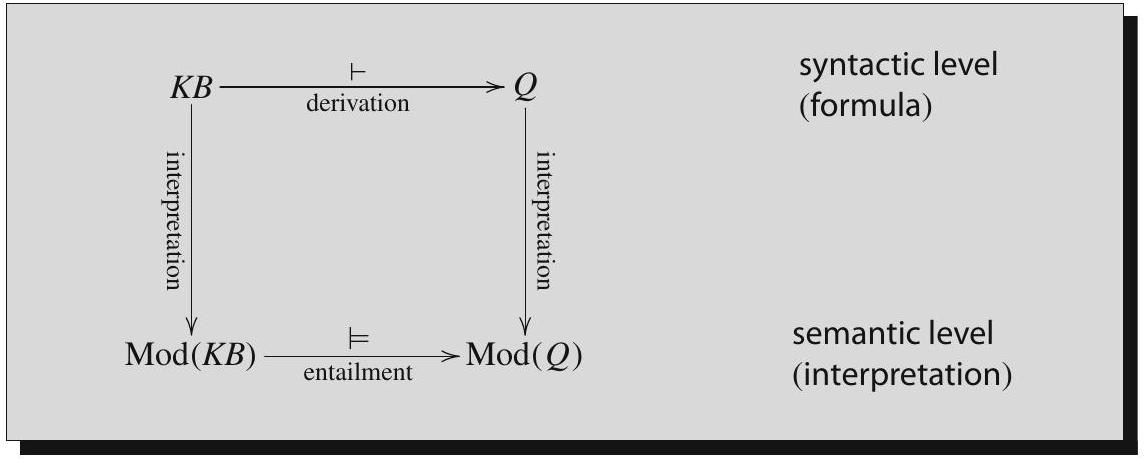
\includegraphics[max width=\textwidth, center]{2025_05_12_af19cd5e0d1b8a465ffeg-035}

Fig. 2.1 Syntactic derivation and semantic entailment. $\operatorname{Mod}(X)$ represents the set of models of a formula $X$\\
the formula to be proved follows from the knowledge base. If a calculus is sound and complete, then syntactic derivation and semantic entailment are two equivalent relations (see Fig. 2.1).

To keep automatic proof systems as simple as possible, these are usually made to operate on formulas in conjunctive normal form.

Definition 2.8 A formula is in conjunctive normal form (CNF) if and only if it consists of a conjunction

$$
K_{1} \wedge K_{2} \wedge \cdots \wedge K_{m}
$$

of clauses. A clause $K_{i}$ consists of a disjunction

$$
\left(L_{i 1} \vee L_{i 2} \vee \cdots \vee L_{i n_{i}}\right)
$$

of literals. Finally, a literal is a variable (positive literal) or a negated variable (negative literal).

The formula $(A \vee B \vee \neg C) \wedge(A \vee B) \wedge(\neg B \vee \neg C)$ is in conjunctive normal form. The conjunctive normal form does not place a restriction on the set of formulas because:

Theorem 2.4 Every propositional logic formula can be transformed into an equivalent conjunctive normal form.

Example 2.1 We put $A \vee B \Rightarrow C \wedge D$ into conjunctive normal form by using the equivalences from Theorem 2.1 on page 26:

$$
\begin{aligned}
A & \vee B \Rightarrow C \wedge D & & \\
& \equiv \neg(A \vee B) \vee(C \wedge D) & & \text { (implication) } \\
& \equiv(\neg A \wedge \neg B) \vee(C \wedge D) & & \text { (de Morgan) } \\
& \equiv(\neg A \vee(C \wedge D)) \wedge(\neg B \vee(C \wedge D)) & & \text { (distributive law) } \\
& \equiv((\neg A \vee C) \wedge(\neg A \vee D)) \wedge((\neg B \vee C) \wedge(\neg B \vee D)) & & \text { (distributive law) } \\
& \equiv(\neg A \vee C) \wedge(\neg A \vee D) \wedge(\neg B \vee C) \wedge(\neg B \vee D) & & \text { (associative law) }
\end{aligned}
$$

We are now only missing a calculus for syntactic proof of propositional logic formulas. We start with the modus ponens, a simple, intuitive rule of inference, which, from the validity of $A$ and $A \Rightarrow B$, allows the derivation of $B$. We write this formally as

$$
\frac{A, \quad A \Rightarrow B}{B} .
$$

This notation means that we can derive the formula(s) below the line from the comma-separated formulas above the line. Modus ponens as a rule by itself, while sound, is not complete. If we add additional rules we can create a complete calculus, which, however, we do not wish to consider here. Instead we will investigate the resolution rule


\begin{equation*}
\frac{A \vee B, \quad \neg B \vee C}{A \vee C} \tag{2.1}
\end{equation*}


as an alternative. The derived clause is called resolvent. Through a simple transformation we obtain the equivalent form

$$
\frac{A \vee B, \quad B \Rightarrow C}{A \vee C} .
$$

If we set $A$ to $f$, we see that the resolution rule is a generalization of the modus ponens. The resolution rule is equally usable if $C$ is missing or if $A$ and $C$ are missing. In the latter case the empty clause can be derived from the contradiction $B \wedge \neg B$ (Exercise 2.7 on page 38).

\subsection*{2.4 Resolution}
We now generalize the resolution rule again by allowing clauses with an arbitrary number of literals. With the literals $A_{1}, \ldots, A_{m}, B, C_{1}, \ldots, C_{n}$ the general resolution rule reads


\begin{equation*}
\frac{\left(A_{1} \vee \cdots \vee A_{m} \vee B\right), \quad\left(\neg B \vee C_{1} \vee \cdots \vee C_{n}\right)}{\left(A_{1} \vee \cdots \vee A_{m} \vee C_{1} \vee \cdots \vee C_{n}\right)} . \tag{2.2}
\end{equation*}


We call the literals $B$ and $\neg B$ complementary. The resolution rule deletes a pair of complementary literals from the two clauses and combines the rest of the literals into a new clause.

To prove that from a knowledge base $K B$, a query $Q$ follows, we carry out a proof by contradiction. Following Theorem 2.3 on page 28 we must show that a contradiction can be derived from $K B \wedge \neg Q$. In formulas in conjunctive normal form, a contradiction appears in the form of two clauses $(A)$ and $(\neg A)$, which lead to the empty clause as their resolvent. The following theorem ensures us that this process really works as desired.

For the calculus to be complete, we need a small addition, as shown by the following example. Let the formula ( $A \vee A$ ) be given as our knowledge base. To show by the resolution rule that from there we can derive ( $A \wedge A$ ), we must show that the empty clause can be derived from $(A \vee A) \wedge(\neg A \vee \neg A)$. With the resolution rule alone, this is impossible. With factorization, which allows deletion of copies of literals from clauses, this problem is eliminated. In the example, a double application of factorization leads to $(A) \wedge(\neg A)$, and a resolution step to the empty clause.

\begin{displayquote}
Theorem 2.5 The resolution calculus for the proof of unsatisfiability of formulas in conjunctive normal form is sound and complete.
\end{displayquote}

Because it is the job of the resolution calculus to derive a contradiction from $K B \wedge \neg Q$, it is very important that the knowledge base $K B$ is consistent:

Definition 2.9 A formula $K B$ is called consistent if it is impossible to derive from it a contradiction, that is, a formula of the form $\phi \wedge \neg \phi$.

Otherwise anything can be derived from $K B$ (see Exercise 2.8 on page 38). This is true not only of resolution, but also for many other calculi.

Of the calculi for automated deduction, resolution plays an exceptional role. Thus we wish to work a bit more closely with it. In contrast to other calculi, resolution has only two inference rules, and it works with formulas in conjunctive normal form. This makes its implementation simpler. A further advantage compared to many calculi lies in its reduction in the number of possibilities for the application of inference rules in every step of the proof, whereby the search space is reduced and computation time decreased.

As an example, we start with a simple logic puzzle that allows the important steps of a resolution proof to be shown.

Example 2.2 Logic puzzle number 7, entitled $A$ charming English family, from the German book [Ber89] reads (translated to English):

Despite studying English for seven long years with brilliant success, I must admit that when I hear English people speaking English I'm totally perplexed. Recently, moved by noble feelings, I picked up three hitchhikers, a father, mother, and daughter, who I quickly realized were English and only spoke English. At each of the sentences that follow I wavered between two possible interpretations. They told me the following (the second possible meaning is in parentheses): The father: "We are going to Spain (we are from Newcastle)." The mother: "We are not going to Spain and are from Newcastle (we stopped in Paris and are not going to Spain)." The daughter: "We are not from Newcastle (we stopped in Paris)." What about this charming English family?

To solve this kind of problem we proceed in three steps: formalization, transformation into normal form, and proof. In many cases formalization is by far the most difficult step because it is easy to make mistakes or forget small details. (Thus practical exercise is very important. See Exercises 2.9-2.11 on page 38.)

Here we use the variables $S$ for "We are going to Spain", $N$ for "We are from Newcastle", and $P$ for "We stopped in Paris" and obtain as a formalization of the three propositions of father, mother, and daughter

$$
(S \vee N) \wedge[(\neg S \wedge N) \vee(P \wedge \neg S)] \wedge(\neg N \vee P) .
$$

Factoring out $\neg S$ in the middle sub-formula brings the formula into CNF in one step. Numbering the clauses with subscripted indices yields

$$
K B \equiv(S \vee N)_{1} \wedge(\neg S)_{2} \wedge(P \vee N)_{3} \wedge(\neg N \vee P)_{4} .
$$

Now we begin the resolution proof, at first still without a query $Q$. An expression of the form " $\operatorname{Res}(m, n)$ : $\langle\text { clause }\rangle_{k}$ " means that $\langle$ clause $\rangle$ is obtained by resolution of clause $m$ with clause $n$ and is numbered $k$.

$$
\begin{array}{ll}
\operatorname{Res}(1,2): & (N)_{5} \\
\operatorname{Res}(3,4): & (P)_{6} \\
\operatorname{Res}(1,4): & (S \vee P)_{7}
\end{array}
$$

We could have derived clause $P$ also from $\operatorname{Res}(4,5)$ or $\operatorname{Res}(2,7)$. Every further resolution step would lead to the derivation of clauses that are already available. Because it does not allow the derivation of the empty clause, it has therefore been shown that the knowledge base is non-contradictory. So far we have derived $N$ and $P$. To show that $\neg S$ holds, we add the clause $(S)_{8}$ to the set of clauses as a negated query. With the resolution step

$$
\operatorname{Res}(2,8): \quad()_{9}
$$

the proof is complete. Thus $\neg S \wedge N \wedge P$ holds. The "charming English family" evidently comes from Newcastle, stopped in Paris, but is not going to Spain.

Example 2.3 Logic puzzle number 28 from [Ber89], entitled The High Jump, reads\\
Three girls practice high jump for their physical education final exam. The bar is set to 1.20 meters. "I bet", says the first girl to the second, "that I will make it over if, and only if, you don't". If the second girl said the same to the third, who in turn said the same to the first, would it be possible for all three to win their bets?

We show through proof by resolution that not all three can win their bets.\\
Formalization:

The first girl's jump succeeds: $A, \quad$ First girl's bet: $(A \Leftrightarrow \neg B)$,\\
the second girl's jump succeeds: $B, \quad$ second girl's bet: $(B \Leftrightarrow \neg C)$,\\
the third girl's jump succeeds: $C . \quad$ third girl's bet: $(C \Leftrightarrow \neg A)$.\\
Claim: the three cannot all win their bets:

$$
Q \equiv \neg((A \Leftrightarrow \neg B) \wedge(B \Leftrightarrow \neg C) \wedge(C \Leftrightarrow \neg A))
$$

It must now be shown by resolution that $\neg Q$ is unsatisfiable.\\
Transformation into CNF: First girl's bet:

$$
(A \Leftrightarrow \neg B) \equiv(A \Rightarrow \neg B) \wedge(\neg B \Rightarrow A) \equiv(\neg A \vee \neg B) \wedge(A \vee B)
$$

The bets of the other two girls undergo analogous transformations, and we obtain the negated claim

$$
\begin{aligned}
\neg Q \equiv & (\neg A \vee \neg B)_{1} \wedge(A \vee B)_{2} \wedge(\neg B \vee \neg C)_{3} \wedge(B \vee C)_{4} \wedge(\neg C \vee \neg A)_{5} \\
& \wedge(C \vee A)_{6} .
\end{aligned}
$$

From there we derive the empty clause using resolution:

$$
\begin{array}{ll}
\operatorname{Res}(1,6): & (C \vee \neg B)_{7} \\
\operatorname{Res}(4,7): & (C)_{8} \\
\operatorname{Res}(2,5): & (B \vee \neg C)_{9} \\
\operatorname{Res}(3,9): & (\neg C)_{10} \\
\operatorname{Res}(8,10): & ()
\end{array}
$$

Thus the claim has been proved.

\subsection*{2.5 Horn Clauses}
A clause in conjunctive normal form contains positive and negative literals and can be represented in the form

$$
\left(\neg A_{1} \vee \cdots \vee \neg A_{m} \vee B_{1} \vee \cdots \vee B_{n}\right)
$$

with the variables $A_{1}, \ldots, A_{m}$ and $B_{1}, \ldots, B_{n}$. This clause can be transformed in two simple steps into the equivalent form

$$
A_{1} \wedge \cdots \wedge A_{m} \Rightarrow B_{1} \vee \cdots \vee B_{n} .
$$

This implication contains the premise, a conjunction of variables and the conclusion, a disjunction of variables. For example, "If the weather is nice and there is snow on the ground, I will go skiing or I will work." is a proposition of this form. The receiver of this message knows for certain that the sender is not going swimming. A significantly clearer statement would be "If the weather is nice and there is snow on the ground, I will go skiing.". The receiver now has definite information. Thus we call clauses with at most one positive literal definite clauses. These clauses have the advantage that they only allow one conclusion and are thus distinctly simpler to interpret. Many relations can be described by clauses of this type. We therefore define

Definition 2.10 Clauses with at most one positive literal of the form

$$
\left(\neg A_{1} \vee \cdots \vee \neg A_{m} \vee B\right) \quad \text { or } \quad\left(\neg A_{1} \vee \cdots \vee \neg A_{m}\right) \quad \text { or } \quad B
$$

or (equivalently)

$$
A_{1} \wedge \cdots \wedge A_{m} \Rightarrow B \quad \text { or } \quad A_{1} \wedge \cdots \wedge A_{m} \Rightarrow f \quad \text { or } \quad B .
$$

are named Horn clauses (after their inventor). A clause with a single positive literal is a fact. In clauses with negative and one positive literal, the positive literal is called the head.

To better understand the representation of Horn clauses, the reader may derive them from the definitions of the equivalences we have currently been using (Exercise 2.12 on page 38).

Horn clauses are easier to handle not only in daily life, but also in formal reasoning, as we can see in the following example. Let the knowledge base consist of the following clauses (the " $\wedge$ " binding the clauses is left out here and in the text that follows):

\begin{verbatim}
(nice_weather) ${ }_{1}$
$(\text { snowfall })_{2}$
(snowfall $\Rightarrow$ snow $)_{3}$
(nice_weather $\wedge$ snow $\Rightarrow$ skiing $)_{4}$
\end{verbatim}

If we now want to know whether skiing holds, this can easily be derived. A slightly generalized modus ponens suffices here as an inference rule:

$$
\frac{A_{1} \wedge \cdots \wedge A_{m}, \quad A_{1} \wedge \cdots \wedge A_{m} \Rightarrow B}{B} .
$$

The proof of "skiing" has the following form ( $\mathrm{MP}\left(i_{1}, \ldots, i_{k}\right.$ ) represents application of the modus ponens on clauses $i_{1}$ to $i_{k}$ :

$$
\begin{array}{ll}
\operatorname{MP}(2,3): & (\text { snow })_{5} \\
\operatorname{MP}(1,5,4): & (\text { skiing })_{6} .
\end{array}
$$

With modus ponens we obtain a complete calculus for formulas that consist of propositional logic Horn clauses. In the case of large knowledge bases, however, modus ponens can derive many unnecessary formulas if one begins with the wrong clauses. Therefore, in many cases it is better to use a calculus that starts with the query and works backward until the facts are reached. Such systems are designated backward chaining, in contrast to forward chaining systems, which start with facts and finally derive the query, as in the above example with the modus ponens.

For backward chaining of Horn clauses, SLD resolution is used. SLD stands for "Selection rule driven linear resolution for definite clauses". In the above example, augmented by the negated query (skiing $\Rightarrow f$ )

\begin{verbatim}
(nice_weather) ${ }_{1}$
$(\text { snowfall })_{2}$
(snowfall $\Rightarrow$ snow $)_{3}$
(nice_weather $\wedge$ snow $\Rightarrow$ skiing $)_{4}$
(skiing $\Rightarrow f$ ) ${ }_{5}$
\end{verbatim}

we carry out SLD resolution beginning with the resolution steps that follow from this clause

$$
\begin{array}{ll}
\operatorname{Res}(5,4): & (\text { nice_weather } \wedge \text { snow } \Rightarrow f)_{6} \\
\operatorname{Res}(6,1): & (\text { snow } \Rightarrow f)_{7} \\
\operatorname{Res}(7,3): & (\text { snowfall } \Rightarrow f)_{8} \\
\operatorname{Res}(8,2): & ()
\end{array}
$$

and derive a contradiction with the empty clause. Here we can easily see "linear resolution", which means that further processing is always done on the currently derived clause. This leads to a great reduction of the search space. Furthermore, the\\
literals of the current clause are always processed in a fixed order (for example, from right to left) ("Selection rule driven"). The literals of the current clause are called subgoal. The literals of the negated query are the goals. The inference rule for one step reads

$$
\frac{A_{1} \wedge \cdots \wedge A_{m} \Rightarrow B_{1}, \quad B_{1} \wedge B_{2} \wedge \cdots \wedge B_{n} \Rightarrow f}{A_{1} \wedge \cdots \wedge A_{m} \wedge B_{2} \wedge \cdots \wedge B_{n} \Rightarrow f} .
$$

Before application of the inference rule, $B_{1}, B_{2}, \ldots, B_{n}$-the current subgoals-must be proved. After the application, $B_{1}$ is replaced by the new subgoal $A_{1} \wedge \cdots \wedge A_{m}$. To show that $B_{1}$ is true, we must now show that $A_{1} \wedge \cdots \wedge A_{m}$ are true. This process continues until the list of subgoals of the current clauses (the so-called goal stack) is empty. With that, a contradiction has been found. If, for a subgoal $\neg B_{i}$, there is no clause with the complementary literal $B_{i}$ as its clause head, the proof terminates and no contradiction can be found. The query is thus unprovable.

SLD resolution plays an important role in practice because programs in the logic programming language PROLOG consist of predicate logic Horn clauses, and their processing is achieved by means of SLD resolution (see Exercise 2.13 on page 38, or Chap. 5).

\subsection*{2.6 Computability and Complexity}
The truth table method, as the simplest semantic proof system for propositional logic, represents an algorithm that can determine every model of any formula in finite time. Thus the sets of unsatisfiable, satisfiable, and valid formulas are decidable. The computation time of the truth table method for satisfiability grows in the worst case exponentially with the number $n$ of variables because the truth table has $2^{n}$ rows. An optimization, the method of semantic trees, avoids looking at variables that do not occur in clauses, and thus saves computation time in many cases, but in the worst case it is likewise exponential.

In resolution, in the worst case the number of derived clauses grows exponentially with the number of initial clauses. To decide between the two processes, we can therefore use the rule of thumb that in the case of many clauses with few variables, the truth table method is preferable, and in the case of few clauses with many variables, resolution will probably finish faster.

The question remains: can proof in propositional logic go faster? Are there better algorithms? The answer: probably not. After all, S. Cook, the founder of complexity theory, has shown that the 3-SAT problem is NP-complete. 3-SAT is the set of all CNF formulas whose clauses have exactly three literals. Thus it is clear that there is probably (modulo the P/NP problem) no polynomial algorithm for 3-SAT, and thus probably not a general one either. For Horn clauses, however, there is an algorithm in which the computation time for testing satisfiability grows only linearly as the number of literals in the formula increases.

\subsection*{2.7 Applications and Limitations}
Theorem provers for propositional logic are part of the developer's everyday toolset in digital technology. For example, the verification of digital circuits and the generation of test patterns for testing of microprocessors in fabrication are some of these tasks. Special proof systems that work with binary decision diagrams (BDD) are also employed as a data structure for processing propositional logic formulas.

In AI, propositional logic is employed in simple applications. For example, simple expert systems can certainly work with propositional logic. However, the variables must all be discrete, with only a few values, and there may not be any cross-relations between variables. Complex logical connections can be expressed much more elegantly using predicate logic.

Probabilistic logic is a very interesting and current combination of propositional logic and probabilistic computation that allows modeling of uncertain knowledge. It is handled thoroughly in Chap. 7.

\subsection*{2.8 Exercises}
\#7 Exercise 2.1 Give a Backus-Naur form grammar for the syntax of propositional logic.

Exercise 2.2 Show that the following formulas are tautologies:\\
(a) $\neg(A \wedge B) \Leftrightarrow \neg A \vee \neg B$\\
(b) $A \Rightarrow B \Leftrightarrow \neg B \Rightarrow \neg A$\\
(c) $((A \Rightarrow B) \wedge(B \Rightarrow A)) \Leftrightarrow(A \Leftrightarrow B)$\\
(d) $(A \vee B) \wedge(\neg B \vee C) \Rightarrow(A \vee C)$

Exercise 2.3 Transform the following formulas into conjunctive normal form:\\
(a) $A \Leftrightarrow B$\\
(b) $A \wedge B \Leftrightarrow A \vee B$\\
(c) $A \wedge(A \Rightarrow B) \Rightarrow B$

Exercise 2.4 Check the following statements for satisfiability or validity.\\
(a) (play\_lottery $\wedge$ six\_right) $\Rightarrow$ winner\\
(b) (play\_lottery $\wedge$ six\_right $\wedge$ (six\_right $\Rightarrow$ win)) $\Rightarrow$ win\\
(c) $\neg$ ( $\neg$ gas\_in\_tank $\wedge$ (gas\_in\_tank $\vee \neg$ car\_starts) $\Rightarrow \neg$ car\_starts)

薬漆 Exercise 2.5 Using the programming language of your choice, program a theorem prover for propositional logic using the truth table method for formulas in conjunctive normal form. To avoid a costly syntax check of the formulas, you may represent clauses as lists or sets of literals, and the formulas as lists or sets of clauses. The program should indicate whether the formula is unsatisfiable, satisfiable, or true, and output the number of different interpretations and models.

\section*{Exercise 2.6}
(a) Show that modus ponens is a valid inference rule by showing that $A \wedge(A \Rightarrow B) \models B$.\\
(b) Show that the resolution rule (2.1) is a valid inference rule.

\begin{itemize}
  \item Exercise 2.7 Show by application of the resolution rule that, in conjunctive normal form, the empty clause is equivalent to the false statement.
  \item Exercise 2.8 Show that, with resolution, one can "derive" any arbitrary clause from a knowledge base that contains a contradiction.
\end{itemize}

Exercise 2.9 Formalize the following logical functions with the logical operators and show that your formula is valid. Present the result in CNF.\\
(a) The XOR operation (exclusive or) between two variables.\\
(b) The statement at least two of the three variables $A, B, C$ are true.

\begin{itemize}
  \item Exercise 2.10 Solve the following case with the help of a resolution proof: "If the criminal had an accomplice, then he came in a car. The criminal had no accomplice and did not have the key, or he had the key and an accomplice. The criminal had the key. Did the criminal come in a car or not?"
\end{itemize}

Exercise 2.11 Show by resolution that the formula from\\
(a) Exercise 2.2(d) is a tautology.\\
(b) Exercise 2.4(c) is unsatisfiable.

Exercise 2.12 Prove the following equivalences, which are important for working with Horn clauses:\\
(a) $\left(\neg A_{1} \vee \cdots \vee \neg A_{m} \vee B\right) \equiv A_{1} \wedge \cdots \wedge A_{m} \Rightarrow B$\\
(b) $\left(\neg A_{1} \vee \cdots \vee \neg A_{m}\right) \equiv A_{1} \wedge \cdots \wedge A_{m} \Rightarrow f$\\
(c) $A \equiv w \Rightarrow A$

Exercise 2.13 Show by SLD resolution that the following Horn clause set is unsatisfiable.

\begin{center}
\begin{tabular}{lll}
$(A)_{1}$ & $(D)_{4}$ & $(A \wedge D \Rightarrow G)_{7}$ \\
$(B)_{2}$ & $(E)_{5}$ & $(C \wedge F \wedge E \Rightarrow H)_{8}$ \\
$(C)_{3}$ & $(A \wedge B \wedge C \Rightarrow F)_{6}$ & $(H \Rightarrow f)_{9}$ \\
\end{tabular}
\end{center}

\# $\rightarrow$ Exercise 2.14 In Sect. 2.6 it says: "Thus it is clear that there is probably (modulo the P/NP problem) no polynomial algorithm for 3-SAT, and thus probably not a general one either." Justify the "probably" in this sentence.

\section*{First-order Predicate Logic}
\section*{3}
Many practical, relevant problems cannot be or can only very inconveniently be formulated in the language of propositional logic, as we can easily recognize in the following example. The statement

\begin{displayquote}
"Robot 7 is situated at the xy position (35, 79)"
\end{displayquote}

can in fact be directly used as the propositional logic variable

\begin{verbatim}
"Robot_7_is_situated_at_xy_position_(35, 79)"
\end{verbatim}

for reasoning with propositional logic, but reasoning with this kind of proposition is very inconvenient. Assume 100 of these robots can stop anywhere on a grid of $100 \times 100$ points. To describe every position of every robot, we would need $100 \cdot 100 \cdot 100=1000000=10^{6}$ different variables. The definition of relationships between objects (here robots) becomes truly difficult. The relation

\begin{displayquote}
"Robot $A$ is to the right of robot $B$."
\end{displayquote}

is semantically nothing more than a set of pairs. Of the 10000 possible pairs of $x$-coordinates there are $(99 \cdot 98) / 2=4851$ ordered pairs. Together with all 10000 combinations of possible $y$-values for both robots, there are $(100 \cdot 99)=9900$ formulas of the type

\begin{verbatim}
Robot_7_is_to_the_right_of_robot_12 $\Leftrightarrow$
    Robot_7_is_situated_at_xy_position_(35, 79)
    $\wedge$ Robot_12_is_situated_at_xy_position_(10, 93) $\vee \ldots$
\end{verbatim}

defining these relations, each of them with $\left(10^{4}\right)^{2} \cdot 0.485=0.485 \cdot 10^{8}$ alternatives on the right side. In first-order predicate logic, we can define a predicate

Position(number, xPosition, yPosition). The above relation must no longer be enumerated as a huge number of pairs, rather it is described abstractly with a rule of the form

\begin{verbatim}
$\forall u \forall v$ is_further_right $(u, v) \Leftrightarrow$
    $\exists x_{u} \exists y_{u} \exists x_{v} \exists y_{v}$ position $\left(u, x_{u}, y_{u}\right) \wedge$ position $\left(v, x_{v}, y_{v}\right) \wedge x_{u}>x_{v}$,
\end{verbatim}

Where $\forall u$ is read as "for every $u$ " and $\exists v$ as "there exists $v$ ".\\
In this chapter we will define the syntax and semantics of first-order predicate logic (PL1), show that many applications can be modeled with this language and that there is a complete and sound calculus for this language.

\subsection*{3.1 Syntax}
First we solidify the syntactic structure of terms.

Definition 3.1 Let $V$ be a set of variables, $K$ a set of constants, and $F$ a set of function symbols. The sets $V, K$ and $F$ are pairwise disjoint. We define the set of terms recursively:

\begin{itemize}
  \item All variables and constants are (atomic) terms.
  \item If $t_{1}, \ldots, t_{n}$ are terms and $f$ an $n$-place function symbol, then $f\left(t_{1}, \ldots, t_{n}\right)$ is also a term.
\end{itemize}

Some examples of terms are $f(\sin (\ln (3)), \exp (x))$ and $g(g(g(x)))$. To be able to establish logical relationships between terms, we build formulas from terms.

Definition 3.2 Let $P$ be a set of predicate symbols. Predicate logic formulas are built as follows:

\begin{itemize}
  \item If $t_{1}, \ldots, t_{n}$ are terms and $p$ an $n$-place predicate symbol, then $p\left(t_{1}, \ldots, t_{n}\right)$ is an (atomic) formula.
  \item If $A$ and $B$ are formulas, then $\neg A,(A), A \wedge B, A \vee B, A \Rightarrow B, A \Leftrightarrow B$ are also formulas.
  \item If $x$ is a variable and $A$ a formula, then $\forall x A$ and $\exists x A$ are also formulas. $\forall$ is the universal quantifier and $\exists$ the existential quantifier.
  \item $p\left(t_{1}, \ldots, t_{n}\right)$ and $\neg p\left(t_{1}, \ldots, t_{n}\right)$ are called literals.
\end{itemize}

Table 3.1 Examples of formulas in first-order predicate logic. Please note that mother here is a function symbol

\begin{center}
\begin{tabular}{|l|l|}
\hline
Formula & Description \\
\hline
$\forall x$ frog $(x) \Rightarrow \operatorname{green}(x)$ & All frogs are green \\
\hline
$\forall x \operatorname{frog}(x) \wedge \operatorname{brown}(x) \Rightarrow \operatorname{big}(x)$ & All brown frogs are big \\
\hline
$\forall x$ likes( $x$, cake) & Everyone likes cake \\
\hline
$\neg \forall x$ likes( $x$, cake) & Not everyone likes cake \\
\hline
$\neg \exists x$ likes( $x$, cake) & No one likes cake \\
\hline
$\exists x \forall y$ likes $(y, x)$ & There is something that everyone likes \\
\hline
$\exists x \forall y$ likes $(x, y)$ & There is someone who likes everything \\
\hline
$\forall x \exists y$ likes $(y, x)$ & Everything is loved by someone \\
\hline
$\forall x \exists y$ likes $(x, y)$ & Everyone likes something \\
\hline
$\forall x$ customer $(x) \Rightarrow$ likes(bob, $x$ ) & Bob likes every customer \\
\hline
$\exists x$ customer $(x) \wedge$ likes $(x$, bob $)$ & There is a customer whom bob likes \\
\hline
$\exists x$ baker $(x) \wedge \forall y$ customer $(y) \Rightarrow \operatorname{likes}(x, y)$ & There is a baker who likes all of his customers \\
\hline
$\forall x$ older(mother( $x$ ), $x$ ) & Every mother is older than her child \\
\hline
$\forall x$ older (mother(mother( $x)$ ), $x$ ) & Every grandmother is older than her daughter's child \\
\hline
$\forall x \forall y \forall z \operatorname{rel}(x, y) \wedge \operatorname{rel}(y, z) \Rightarrow \operatorname{rel}(x, z)$ & rel is a transitive relation \\
\hline
\end{tabular}
\end{center}

\begin{itemize}
  \item Formulas in which every variable is in the scope of a quantifier are called first-order sentences or closed formulas. Variables which are not in the scope of a quantifier are called free variables.
  \item Definitions 2.8 (CNF) and 2.10 (Horn clauses) hold for formulas of predicate logic literals analogously.
\end{itemize}

In Table 3.1 several examples of PL1 formulas are given along with their intuitive interpretations.

\subsection*{3.2 Semantics}
In propositional logic, every variable is directly assigned a truth value by an interpretation. In predicate logic, the meaning of formulas is recursively defined over the construction of the formula, in that we first assign constants, variables, and function symbols to objects in the real world.

Definition 3.3 An interpretation II is defined as

\begin{itemize}
  \item A mapping from the set of constants and variables $K \cup V$ to a set $W$ of names of objects in the world.
  \item A mapping from the set of function symbols to the set of functions in the world. Every $n$-place function symbol is assigned an $n$-place function.
  \item A mapping from the set of predicate symbols to the set of relations in the world. Every $n$-place predicate symbol is assigned an $n$-place relation.
\end{itemize}

Example 3.1 Let $c_{1}, c_{2}, c_{3}$ be constants, "plus" a two-place function symbol, and " $g r$ " a two-place predicate symbol. The truth of the formula

$$
F \equiv \operatorname{gr}\left(p l u s\left(c_{1}, c_{3}\right), c_{2}\right)
$$

depends on the interpretation $\mathbb{I}$. We first choose the following obvious interpretation of constants, the function, and of the predicates in the natural numbers:

$$
\mathbb{I}_{1}: c_{1} \mapsto 1, c_{2} \mapsto 2, c_{3} \mapsto 3, \quad \text { plus } \mapsto+, \quad g r \mapsto>.
$$

Thus the formula is mapped to

$$
1+3>2, \quad \text { or after evaluation } \quad 4>2 .
$$

The greater-than relation on the set $\{1,2,3,4\}$ is the set of all pairs $(x, y)$ of numbers with $x>y$, meaning the set $G=\{(4,3),(4,2),(4,1),(3,2),(3,1),(2,1)\}$. Because $(4,2) \in G$, the formula $F$ is true under the interpretation $\mathbb{I}_{1}$. However, if we choose the interpretation

$$
\mathbb{I}_{2}: c_{1} \mapsto 2, c_{2} \mapsto 3, c_{3} \mapsto 1, \quad \text { plus } \mapsto-, \quad g r \mapsto>,
$$

we obtain

$$
2-1>3, \text { or } 1>3 .
$$

The pair $(1,3)$ is not a member of $G$. The formula $F$ is false under the interpretation $\mathbb{I}_{2}$. Obviously, the truth of a formula in PL1 depends on the interpretation. Now, after this preview, we define truth.

\section*{Definition 3.4}
\begin{itemize}
  \item An atomic formula $p\left(t_{1}, \ldots, t_{n}\right)$ is true (or valid) under the interpretation $\mathbb{I}$ if, after interpretation and evaluation of all terms $t_{1}, \ldots, t_{n}$ and interpretation of the predicate $p$ through the $n$-place relation $r$, it holds that
\end{itemize}

$$
\left(\mathbb{I}\left(t_{1}\right), \ldots, \mathbb{I}\left(t_{n}\right)\right) \in r .
$$

\begin{itemize}
  \item The truth of quantifierless formulas follows from the truth of atomic formulas-as in propositional calculus-through the semantics of the logical operators defined in Table 2.1 on page 25.
  \item A formula $\forall x F$ is true under the interpretation $\mathbb{I}$ exactly when it is true given an arbitrary change of the interpretation for the variable $x$ (and only for $x$ )
  \item A formula $\exists x F$ is true under the interpretation $\mathbb{I}$ exactly when there is an interpretation for $x$ which makes the formula true.\\
The definitions of semantic equivalence of formulas, for the concepts satisfiable, true, unsatisfiable, and model, along with semantic entailment (Definitions 2.4, 2.5, 2.6) carry over unchanged from propositional calculus to predicate logic.
\end{itemize}

Theorem 3.1 Theorems 2.2 (deduction theorem) and 2.3 (proof by contradiction) hold analogously for PL1.

Example 3.2 The family tree given in Fig. 3.1 graphically represents (in the semantic level) the relation\\
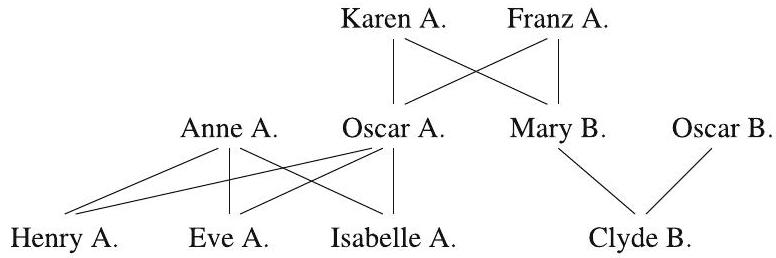
\includegraphics[max width=\textwidth, center]{2025_05_12_af19cd5e0d1b8a465ffeg-049}

Fig. 3.1 A family tree. The edges going from Clyde B. upward to Mary B. and Oscar B. represent the element (Clyde B., Mary B., Oscar B.) as a child relationship

\begin{center}
\begin{tabular}{rl}
Child $=$ & \begin{tabular}{rl}
$($ & Oscar A., Karen A., Frank A. $),$ \\
 & $($ Henry A., Anne A., Oscar A. $)$, \\
 & $($ Isabelle A., Anne A., Oscar A. $)$, \\
\end{tabular} \\
 & $($ Mary B., Karen A., Frank A. $)$, \\
 & $($ Eve A., Anne A., Oscar A. $)$, \\
 & $($ Clyde B., Mary B., Oscar B. $)\}$ \\
\end{tabular}
\end{center}

For example, the triple (Oscar A., Karen A., Frank A.) stands for the proposition "Oscar A. is a child of Karen A. and Frank A.". From the names we read off the one-place relation

$$
\text { Female }=\{\text { Karen A., Anne A., Mary B., Eve A., Isabelle A. }\}
$$

of the women. We now want to establish formulas for family relationships. First we define a three-place predicate $\operatorname{child}(x, y, z)$ with the semantic

$$
\mathbb{I}(\operatorname{child}(x, y, z))=w \equiv(\mathbb{I}(x), \mathbb{I}(y), \mathbb{I}(z)) \in \operatorname{Kind} .
$$

Under the interpretation $\mathbb{I}($ oscar $)=$ Oscar A., $\mathbb{I}($ eve $)=$ Eve A., $\mathbb{I}($ anne $)=$ Anne A., it is also true that child(eve, anne, oscar). For child(eve, oscar, anne) to be true, we require, with

$$
\forall x \forall y \forall z \operatorname{child}(x, y, z) \Leftrightarrow \operatorname{child}(x, z, y),
$$

symmetry of the predicate child in the last two arguments. For further definitions we refer to Exercise 3.1 on page 63 and define the predicate descendant recursively as

$$
\begin{aligned}
\forall x \forall y \text { descendant }(x, y) \Leftrightarrow & \exists z \operatorname{child}(x, y, z) \vee \\
& (\exists u \exists v \operatorname{child}(x, u, v) \wedge \operatorname{descendant}(u, y)) .
\end{aligned}
$$

Now we build a small knowledge base with rules and facts. Let

$$
\begin{aligned}
K B \equiv & \text { female }(\text { karen }) \wedge \text { female }(\text { anne }) \wedge \text { female }(\text { mary }) \\
& \wedge \text { female }(\text { eve }) \wedge \text { female }(\text { isabelle }) \\
& \wedge \text { child }(\text { oscar }, \text { karen, } \text { franz }) \wedge \text { child }(\text { mary }, \text { karen }, \text { franz }) \\
& \wedge \text { child }(\text { eve }, \text { anne }, \text { oscar }) \wedge \text { child }(\text { henry }, \text { anne }, \text { oscar }) \\
& \wedge \text { child }(\text { isabelle }, \text { anne }, \text { oscar }) \wedge \text { child }(\text { clyde }, \text { mary }, \text { oscar }) \\
& \wedge(\forall x \forall y \forall z \text { child }(x, y, z) \Rightarrow \text { child }(x, z, y)) \\
& \wedge(\forall x \forall y \text { descendant }(x, y) \Leftrightarrow \exists z \text { child }(x, y, z) \\
& \vee(\exists u \exists \text { vchild }(x, u, v) \wedge \text { descendant }(u, y)))
\end{aligned}
$$

We can now ask, for example, whether the propositions child(eve, oscar, anne) or descendant(eve, franz) are derivable. To that end we require a calculus.

\subsection*{3.2.1 Equality}
To be able to compare terms, equality is a very important relation in predicate logic. The equality of terms in mathematics is an equivalence relation, meaning it is reflexive, symmetric and transitive. If we want to use equality in formulas, we must either incorporate these three attributes as axioms in our knowledge base, or we must integrate equality into the calculus. We take the easy way and define a predicate " $=$ " which, deviating from Definition 3.2 on page 40, is written using infix notation as is customary in mathematics. (An equation $x=y$ could of course also be written in the form $e q(x, y)$.) Thus, the equality axioms have the form

\[
\begin{array}{rll}
\forall x & x=x & \text { (reflexivity) } \\
\forall x \forall y & x=y \Rightarrow y=x & \text { (symmetry) }  \tag{3.1}\\
\forall x \forall y \forall z & x=y \wedge y=z \Rightarrow x=z & \text { (transitivity). }
\end{array}
\]

To guarantee the uniqueness of functions, we additionally require


\begin{equation*}
\forall x \forall y x=y \Rightarrow f(x)=f(y) \quad \text { (substitution axiom) } \tag{3.2}
\end{equation*}


for every function symbol. Analogously we require for all predicate symbols


\begin{equation*}
\forall x \forall y x=y \Rightarrow p(x) \Leftrightarrow p(y) \quad \text { (substitution axiom). } \tag{3.3}
\end{equation*}


We formulate other mathematical relations, such as the "<" relation, by similar means (Exercise 3.4 on page 64).

Often a variable must be replaced by a term. To carry this out correctly and describe it simply, we give the following definition.

Definition 3.5 We write $\varphi[x / t]$ for the formula that results when we replace every free occurrence of the variable $x$ in $\varphi$ with the term $t$. Thereby we do not allow any variables in the term $t$ that are quantified in $\varphi$. In those cases variables must be renamed to ensure this.

Example 3.3 If, in the formula $\forall x x=y$, the free variable $y$ is replaced by the term $x+1$, the result is $\forall x x=x+1$. With correct substitution we obtain the formula $\forall x x=y+1$, which has a very different semantic.

\subsection*{3.3 Quantifiers and Normal Forms}
By Definition 3.4 on page 43, the formula $\forall x p(x)$ is true if and only if it is true for all interpretations of the variable $x$. Instead of the quantifier, one could write $p\left(a_{1}\right) \wedge \cdots \wedge p\left(a_{n}\right)$ for all constants $a_{1} \cdots a_{n}$ in $K$. For $\exists x p(x)$ one could write $p\left(a_{1}\right) \vee \cdots \vee p\left(a_{n}\right)$. From this it follows with de Morgan's law that

$$
\forall x \varphi \equiv \neg \exists x \neg \varphi .
$$

Through this equivalence, universal, and existential quantifiers are mutually replaceable.

Example 3.4 The proposition "Everyone wants to be loved" is equivalent to the proposition "Nobody does not want to be loved".

Quantifiers are an important component of predicate logic's expressive power. However, they are disruptive for automatic inference in AI because they make the structure of formulas more complex and increase the number of applicable inference rules in every step of a proof. Therefore our next goal is to find, for every predicate logic formula, an equivalent formula in a standardized normal form with as few quantifiers as possible. As a first step we bring universal quantifiers to the beginning of the formula and thus define

Definition 3.6 A predicate logic formula $\varphi$ is in prenex normal form if it holds that

\begin{itemize}
  \item $\varphi=Q_{1} x_{1} \cdots Q_{n} x_{n} \psi$.
  \item $\psi$ is a quantifierless formula.
  \item $Q_{i} \in\{\forall, \exists\}$ for $i=1, \ldots, n$.
\end{itemize}

Caution is advised if a quantified variable appears outside the scope of its quantifier, as for example $x$ in

$$
\forall x p(x) \Rightarrow \exists x q(x)
$$

Here one of the two variables must be renamed, and in

$$
\forall x p(x) \Rightarrow \exists y q(y)
$$

the quantifier can easily be brought to the front, and we obtain as output the equivalent formula

$$
\forall x \exists y p(x) \Rightarrow q(y)
$$

If, however, we wish to correctly bring the quantifier to the front of


\begin{equation*}
(\forall x p(x)) \Rightarrow \exists y q(y) \tag{3.4}
\end{equation*}


we first write the formula in the equivalent form

$$
\neg(\forall x p(x)) \vee \exists y q(y) .
$$

The first universal quantifier now turns into

$$
(\exists x \neg p(x)) \vee \exists y q(y)
$$

and now the two quantifiers can finally be pulled forward to

$$
\exists x \exists y \neg p(x) \vee q(y),
$$

which is equivalent to

$$
\exists x \exists y p(x) \Rightarrow q(y)
$$

We see then that in (3.4) on page 46 we cannot simply pull both quantifiers to the front. Rather, we must first eliminate the implications so that there are no negations on the quantifiers. It holds in general that we may only pull quantifiers out if negations only exist directly on atomic sub-formulas.

Example 3.5 As is well known in analysis, convergence of a series $\left(a_{n}\right)_{n \in \mathbb{N}}$ to a limit $a$ is defined by

$$
\forall \varepsilon>0 \exists n_{0} \in \mathbb{N} \forall n>n_{0}\left|a_{n}-a\right|<\varepsilon
$$

With the function $\operatorname{abs}(x)$ for $|x|, a(n)$ for $a_{n}$, minus $(x, y)$ for $x-y$ and the predicates $e l(x, y)$ for $x \in y, g r(x, y)$ for $x>y$, the formula reads


\begin{equation*}
\forall \varepsilon\left(g r(\varepsilon, 0) \Rightarrow \exists n_{0}\left(e l\left(n_{0}, \mathbb{N}\right) \Rightarrow \forall n\left(g r\left(n, n_{0}\right) \Rightarrow g r(\varepsilon, \operatorname{abs}(\operatorname{minus}(a(n), a)))\right)\right)\right) \tag{3.5}
\end{equation*}


This is clearly not in prenex normal form. Because the variables of the inner quantifiers $\exists n_{0}$ and $\forall n$ do not occur to the left of their respective quantifiers, no variables must be renamed. Next we eliminate the implications and obtain

$$
\forall \varepsilon\left(\neg g r(\varepsilon, 0) \vee \exists n_{0}\left(\neg e l\left(n_{0}, \mathbb{N}\right) \vee \forall n\left(\neg g r\left(n, n_{0}\right) \vee g r(\varepsilon, a b s(\operatorname{minus}(a(n), a)))\right)\right)\right) .
$$

Because every negation is in front of an atomic formula, we bring the quantifiers forward, eliminate the redundant parentheses, and with

$$
\forall \varepsilon \exists n_{0} \forall n\left(\neg g r(\varepsilon, 0) \vee \neg e l\left(n_{0}, \mathbb{N}\right) \vee \neg g r\left(n, n_{0}\right) \vee g r(\varepsilon, \operatorname{abs}(\operatorname{minus}(a(n), a)))\right)
$$

it becomes a quantified clause in conjunctive normal form.

The transformed formula is equivalent to the output formula. The fact that this transformation is always possible is guaranteed by

Theorem 3.2 Every predicate logic formula can be transformed into an equivalent formula in prenex normal form.

In addition, we can eliminate all existential quantifiers. However, the formula resulting from the so-called Skolemization is no longer equivalent to the output formula. Its satisfiability, however, remains unchanged. In many cases, especially when one wants to show the unsatisfiability of $K B \wedge \neg Q$, this is sufficient. The following formula in prenex normal form will now be skolemized:

$$
\forall x_{1} \forall x_{2} \exists y_{1} \forall x_{3} \exists y_{2} p\left(f\left(x_{1}\right), x_{2}, y_{1}\right) \vee q\left(y_{1}, x_{3}, y_{2}\right) .
$$

Because the variable $y_{1}$ apparently depends on $x_{1}$ and $x_{2}$, every occurrence of $y_{1}$ is replaced by a Skolem function $g\left(x_{1}, x_{2}\right)$. It is important that $g$ is a new function symbol that has not yet appeared in the formula. We obtain

$$
\forall x_{1} \forall x_{2} \forall x_{3} \exists y_{2} p\left(f\left(x_{1}\right), x_{2}, g\left(x_{1}, x_{2}\right)\right) \vee q\left(g\left(x_{1}, x_{2}\right), x_{3}, y_{2}\right)
$$

and replace $y_{2}$ analogously by $h\left(x_{1}, x_{2}, x_{3}\right)$, which leads to

$$
\forall x_{1} \forall x_{2} \forall x_{3} p\left(f\left(x_{1}\right), x_{2}, g\left(x_{1}, x_{2}\right)\right) \vee q\left(g\left(x_{1}, x_{2}\right), x_{3}, h\left(x_{1}, x_{2}, x_{3}\right)\right) .
$$

Because now all the variables are universally quantified, the universal quantifiers can be left out, resulting in

$$
p\left(f\left(x_{1}\right), x_{2}, g\left(x_{1}, x_{2}\right)\right) \vee q\left(g\left(x_{1}, x_{2}\right), x_{3}, h\left(x_{1}, x_{2}, x_{3}\right)\right)
$$

Now we can eliminate the existential quantifier (and thereby also the universal quantifier) in (3.5) on page 47 by introducing the Skolem function $n_{0}(\varepsilon)$. The skolemized prenex and conjunctive normal form of (3.5) on page 47 thus reads

$$
\neg g r(\varepsilon, 0) \vee \neg e l\left(n_{0}(\varepsilon), \mathbb{N}\right) \vee \neg g r\left(n, n_{0}(\varepsilon)\right) \vee g r(\varepsilon, a b s(\operatorname{minus}(a(n), a))) .
$$

By dropping the variable $n_{0}$, the Skolem function can receive the name $n_{0}$.\\
When skolemizing a formula in prenex normal form, all existential quantifiers are eliminated from the outside inward, where a formula of the form $\forall x_{1} \ldots \forall x_{n} \exists y \varphi$ is replaced by $\forall x_{1} \ldots \forall x_{n} \varphi\left[y / f\left(x_{1}, \ldots, x_{n}\right)\right]$, during which $f$ may not appear in $\varphi$. If an existential quantifier is on the far outside, such as in $\exists y p(y)$, then $y$ must be replaced by a constant (that is, by a zero-place function symbol).\\
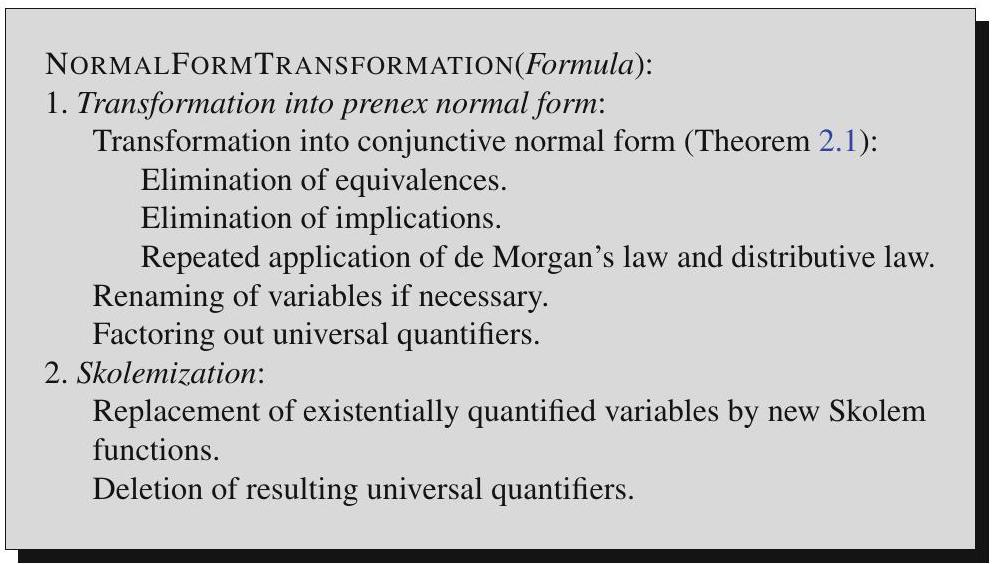
\includegraphics[max width=\textwidth, center]{2025_05_12_af19cd5e0d1b8a465ffeg-055}

Fig. 3.2 Transformation of predicate logic formulas into normal form

The procedure for transforming a formula in conjunctive normal form is summarized in the pseudocode represented in Fig. 3.2. Skolemization has polynomial runtime in the number of literals. When transforming into normal form, the number of literals in the normal form can grow exponentially, which can lead to exponential computation time and exponential memory usage. The reason for this is the repeated application of the distributive law. The actual problem, which results from a large number of clauses, is the combinatorial explosion of the search space for a subsequent resolution proof. However, there is an optimized transformation algorithm which only spawns polynomially many literals [Ede91].

\subsection*{3.4 Proof Calculi}
For reasoning in predicate logic, various calculi of natural reasoning such as Gentzen calculus or sequent calculus, have been developed. As the name suggests, these calculi are meant to be applied by humans, since the inference rules are more or less intuitive and the calculi work on arbitrary PL1 formulas. In the next section we will primarily concentrate on the resolution calculus, which is in practice the most important efficient, automatizable calculus for formulas in conjunctive normal form. Here, using Example 3.2 on page 43 we will give a very small "natural" proof. We use the inference rule

$$
\frac{A, \quad A \Rightarrow B}{B} \quad \text { (modus ponens, MP) and } \frac{\forall x A}{A[x / t]} \quad(\forall \text {-elimination, } \forall E) \text {. }
$$

The modus ponens is already familiar from propositional logic. When eliminating universal quantifiers one must keep in mind that the quantified variable $x$ must be

Table 3.2 Simple proof with modus ponens and quantifier elimination

\begin{center}
\begin{tabular}{lll}
\hline
WB: & 1 & child(eve, anne, oscar) \\
\hline
WB: & 2 & $\forall x \forall y \forall z$ child $(x, y, z) \Rightarrow$ child $(x, z, y)$ \\
\hline
$\forall E(2):$ x/eve, ylanne,$z$ loscar & 3 & child $($ eve, anne, oscar $) \Rightarrow$ child $($ eve, oscar, anne $)$ \\
\hline
$M P(1,3)$ & 4 & child $($ eve, oscar, anne $)$ \\
\hline
\end{tabular}
\end{center}

replaced by a ground term $t$, meaning a term that contains no variables. The proof of child(eve, oscar, anne) from an appropriately reduced knowledge base is presented in Table 3.2.

The two formulas of the reduced knowledge base are listed in rows 1 and 2. In row 3 the universal quantifiers from row 2 are eliminated, and in row 4 the claim is derived with modus ponens.

The calculus consisting of the two given inference rules is not complete. However, it can be extended into a complete procedure by addition of further inference rules. This nontrivial fact is of fundamental importance for mathematics and AI. The Austrian logician Kurt Gödel proved in 1931 that [Göd31a].

Theorem 3.3 (Gödel's completeness theorem) First-order predicate logic is complete. That is, there is a calculus with which every proposition that is a consequence of a knowledge base $K B$ can be proved. If $K B \models \varphi$, then it holds that $K B \vdash \varphi$.

Every true proposition in first-order predicate logic is therefore provable. But is the reverse also true? Is everything we can derive syntactically actually true? The answer is "yes":

Theorem 3.4 (Correctness) There are calculi with which only true propositions can be proved. That is, if $K B \vdash \varphi$ holds, then $K B \models \varphi$.

In fact, nearly all known calculi are correct. After all, it makes little sense to work with incorrect proof methods. Provability and semantic consequence are therefore equivalent concepts, as long as correct and complete calculus is being used. Thereby first-order predicate logic becomes a powerful tool for mathematics and AI. The aforementioned calculi of natural deduction are rather unsuited for automatization. Only resolution calculus, which was introduced in 1965 and essentially works with only one simple inference rule, enabled the construction of powerful automated theorem provers, which later were employed as inference machines for expert systems.

\subsection*{3.5 Resolution}
Indeed, the correct and complete resolution calculus triggered a logic euphoria during the 1970s. Many scientists believed that one could formulate almost every task of knowledge representation and reasoning in PL1 and then solve it with an automated prover. Predicate logic, a powerful, expressive language, together with a complete proof calculus seemed to be the universal intelligent machine for representing knowledge and solving many difficult problems (Fig. 3.3).

If one feeds a set of axioms (that is, a knowledge base) and a query into such a logic machine as input, the machine searches for a proof and returns it-for one exists and will be found-as output. With Gödel's completeness theorem and the work of Herbrand as a foundation, much was invested into the mechanization of logic. The vision of a machine that could, with an arbitrary non-contradictory PL1 knowledge base, prove any true query was very enticing. Accordingly, until now many proof calculi for PL1 are being developed and realized in the form of theorem provers. As an example, here we describe the historically important and widely used resolution calculus and show its capabilities. The reason for selecting resolution as an example of a proof calculus in this book is, as stated, its historical and\\
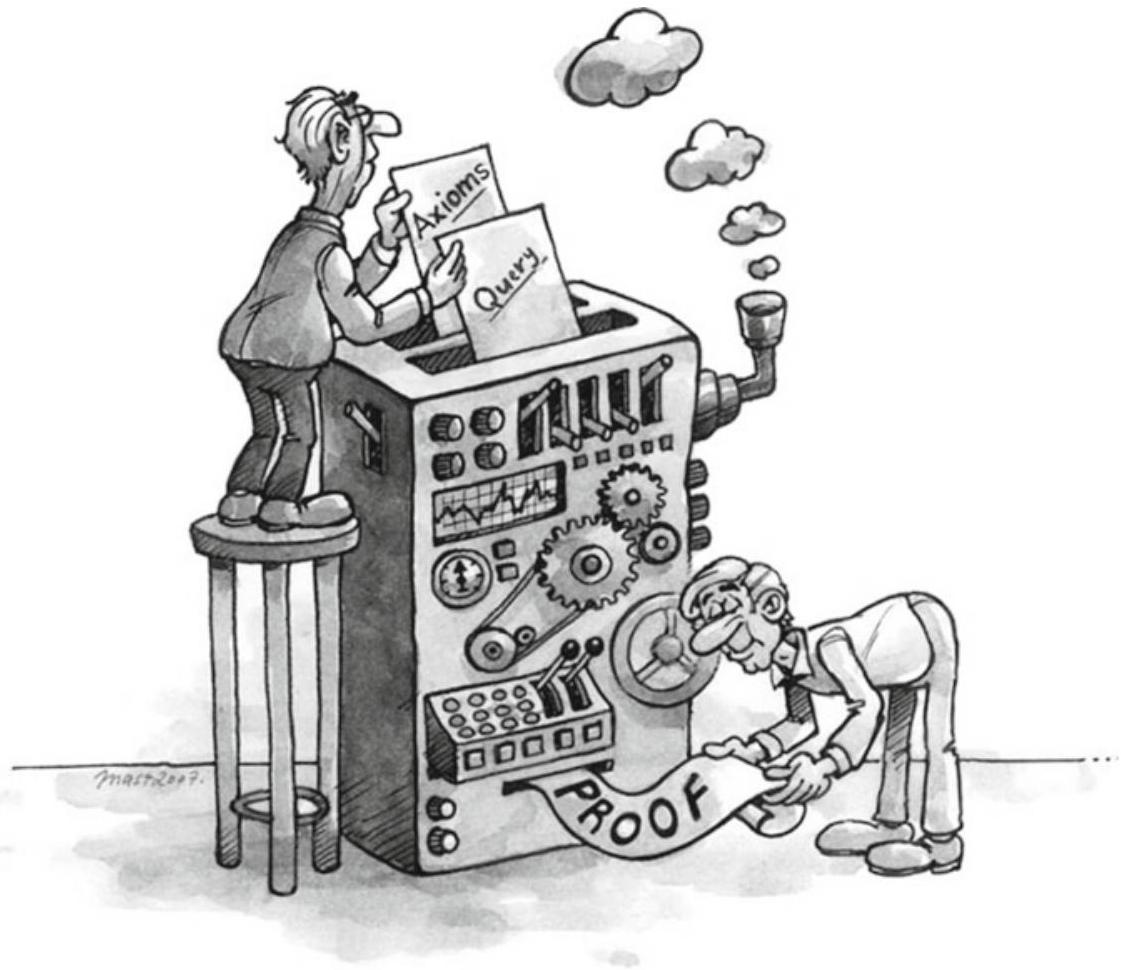
\includegraphics[max width=\textwidth, center]{2025_05_12_af19cd5e0d1b8a465ffeg-057}

Fig. 3.3 The universal logic machine\\
didactic importance. Today, resolution represents just one of many calculi used in high-performance provers.

We begin by trying to compile the proof in Table 3.2 on page 50 with the knowledge base of Example 3.2 on page 43 into a resolution proof. First the formulas are transformed into conjunctive normal form and the negated query

$$
\neg Q \equiv \neg \text { child(eve, oscar, anne) }
$$

is added to the knowledge base, which gives

$$
\begin{aligned}
K B \wedge \neg Q \equiv & (\text { child }(\text { eve }, \text { anne }, \text { oscar }))_{1} \wedge \\
& (\neg \text { child }(x, y, z) \vee \text { child }(x, z, y))_{2} \wedge \\
& (\neg \text { child }(\text { eve }, \text { oscar }, \text { anne }))_{3} .
\end{aligned}
$$

The proof could then look something like

$$
\text { (2) } \begin{aligned}
x / \text { eve }, y / \text { anne }, z / \text { oscar }: & (\neg \text { child }(\text { eve }, \text { anne }, \text { oscar }) \vee \\
& \text { child }(\text { eve }, \text { oscar }, \text { anne }))_{4} \\
\operatorname{Res}(3,4): & (\neg \text { child }(\text { eve }, \text { anne }, \text { oscar }))_{5} \\
\operatorname{Res}(1,5): & ()_{6},
\end{aligned}
$$

where, in the first step, the variables $x, y, z$ are replaced by constants. Then two resolution steps follow under application of the general resolution rule from (2.2), which was taken unchanged from propositional logic.

The circumstances in the following example are somewhat more complex. We assume that everyone knows his own mother and ask whether Henry knows anyone. With the function symbol "mother" and the predicate "knows", we have to derive a contradiction from

$$
(\text { knows }(x, \text { mother }(x)))_{1} \wedge(\neg \text { knows }(\text { henry }, y))_{2} .
$$

By the replacement $x$ /henry, $y$ /mother (henry) we obtain the contradictory clause pair

$$
(\text { knows }(\text { henry }, \text { mother }(\text { henry })))_{1} \wedge(\neg \text { knows }(\text { henry }, \text { mother }(\text { henry })))_{2} .
$$

This replacement step is called unification. The two literals are complementary, which means that they are the same other than their signs. The empty clause is now derivable with a resolution step, by which it has been shown that Henry does know someone (his mother). We define

Definition 3.7 Two literals are called unifiable if there is a substitution $\sigma$ for all variables which makes the literals equal. Such a $\sigma$ is called a unifier. A unifier is called the most general unifier (MGU) if all other unifiers can be obtained from it by substitution of variables.

Example 3.6 We want to unify the literals $p(f(g(x)), y, z)$ and $p(u, u, f(u))$. Several unifiers are

\begin{center}
\begin{tabular}{lllll}
$\sigma_{1}:$ & $y / f(g(x))$, & $z / f(f(g(x)))$, & $u / f(g(x))$, &  \\
$\sigma_{2}:$ & $x / h(v)$, & $y / f(g(h(v)))$, & $z / f(f(g(h(v))))$, & $u / f(g(h(v)))$ \\
$\sigma_{3}:$ & $x / h(h(v))$, & $y / f(g(h(h(v))))$, & $z / f(f(g(h(h(v)))))$, & $u / f(g(h(h(v))))$ \\
$\sigma_{4}:$ & $x / h(a)$, & $y / f(g(h(a)))$, & $z / f(f(g(h(a))))$, & $u / f(g(h(a)))$ \\
$\sigma_{5}:$ & $x / a$, & $y / f(g(a))$, & $z / f(f(g(a)))$, & $u / f(g(a))$ \\
\end{tabular}
\end{center}

where $\sigma_{1}$ is the most general unifier. The other unifiers result from $\sigma_{1}$ through the substitutions $x / h(v), x / h(h(v)), x / h(a), x / a$.

We can see in this example that during unification of literals, the predicate symbols can be treated like function symbols. That is, the literal is treated like a term. Implementations of unification algorithms process the arguments of functions sequentially. Terms are unified recursively over the term structure. The simplest unification algorithms are very fast in most cases. In the worst case, however, the computation time can grow exponentially with the size of the terms. Because for automated provers the overwhelming number of unification attempts fail or are very simple, in most cases the worst case complexity has no dramatic effect. The fastest unification algorithms have nearly linear complexity even in the worst case [Bib82].

We can now give the general resolution rule for predicate logic:

Definition 3.8 The resolution rule for two clauses in conjunctive normal form reads


\begin{equation*}
\frac{\left(A_{1} \vee \cdots \vee A_{m} \vee B\right), \quad\left(\neg B^{\prime} \vee C_{1} \vee \cdots \vee C_{n}\right) \quad \sigma(B)=\sigma\left(B^{\prime}\right)}{\left(\sigma\left(A_{1}\right) \vee \cdots \vee \sigma\left(A_{m}\right) \vee \sigma\left(C_{1}\right) \vee \cdots \vee \sigma\left(C_{n}\right)\right)}, \tag{3.6}
\end{equation*}


where $\sigma$ is the MGU of $B$ and $B^{\prime}$.

Theorem 3.5 The resolution rule is correct. That is, the resolvent is a semantic consequence of the two parent clauses.

For Completeness, however, we still need a small addition, as is shown in the following example.

Example 3.7 The famous Russell paradox reads "There is a barber who shaves everyone who does not shave himself." This statement is contradictory, meaning it is unsatisfiable. We wish to show this with resolution. Formalized in PL1, the paradox reads

$$
\forall x \text { shaves }(\text { barber }, x) \Leftrightarrow \neg \operatorname{shaves}(x, x)
$$

and transformation into clause form yields (see Exercise 3.6 on page 64)\\
$(\neg \text { shaves }(\text { barbier }, x) \vee \neg \text { shaves }(x, x))_{1} \wedge(\text { shaves }(\text { barbier }, x) \vee \text { shaves }(x, x))_{2}$.

From these two clauses we can derive several tautologies, but no contradiction. Thus resolution is not complete. We need yet a further inference rule.

Definition 3.9 Factorization of a clause is accomplished by

$$
\frac{\left(A_{1} \vee A_{2} \vee \cdots \vee A_{n}\right) \quad \sigma\left(A_{1}\right)=\sigma\left(A_{2}\right)}{\left(\sigma\left(A_{2}\right) \vee \cdots \vee \sigma\left(A_{n}\right)\right)},
$$

where $\sigma$ is the MGU of $A_{1}$ and $A_{2}$.

Now a contradiction can be derived from (3.7)

$$
\begin{aligned}
\operatorname{Fak}(1, \sigma: x / \text { barber }): & (\neg \text { shaves }(\text { barber }, \text { barber }))_{3} \\
\operatorname{Fak}(2, \sigma: x / \text { barber }): & (\text { shaves }(\text { barber }, \text { barber }))_{4} \\
\operatorname{Res}(3,4): & ()_{5}
\end{aligned}
$$

and we assert:

Theorem 3.6 The resolution rule (3.6) together with the factorization rule (3.9) is refutation complete. That is, by application of factorization and resolution steps, the empty clause can be derived from any unsatisfiable formula in conjunctive normal form.

\subsection*{3.5.1 Resolution Strategies}
While completeness of resolution is important for the user, the search for a proof can be very frustrating in practice. The reason for this is the immense combinatorial search space. Even if there are only very few pairs of clauses in $K B \wedge \neg Q$ in the beginning, the prover generates a new clause with every resolution step, which increases the number of possible resolution steps in the next iteration. Thus it has long been attempted to reduce the search space using special strategies, preferably without losing completeness. The most important strategies are the following.

Unit resolution prioritizes resolution steps in which one of the two clauses consists of only one literal, called a unit clause. This strategy preserves completeness and leads in many cases, but not always, to a reduction of the search space. It therefore is a heuristic process (see Sect. 6.3).

One obtains a guaranteed reduction of the search space by application of the set of support strategy. Here a subset of $K B \wedge \neg Q$ is defined as the set of support (SOS). Every resolution step must involve a clause from the SOS, and the resolvent is added to the SOS. This strategy is incomplete. It becomes complete when it is ensured that the set of clauses is satisfiable without the SOS (see Exercise 3.7 on page 64). The negated query $\neg Q$ is often used as the initial SOS.

In input resolution, a clause from the input set $K B \wedge \neg Q$ must be involved in every resolution step. This strategy also reduces the search space, but at the cost of completeness.

With the pure literal rule all clauses that contain literals for which there are no complementary literals in other clauses can be deleted. This rule reduces the search space and is complete, and therefore it is used by practically all resolution provers.

If the literals of a clause $K_{1}$ represent a subset of the literals of the clause $K_{2}$, then $K_{2}$ can be deleted. For example, the clause

$$
(\text { raining }(\text { today }) \Rightarrow \text { street_wet }(\text { today }))
$$

is redundant if street\_wet(today) is already valid. This important reduction step is called subsumption. Subsumption, too, is complete.

\subsection*{3.5.2 Equality}
Equality is an especially inconvenient cause of explosive growth of the search space. If we add (3.1) on page 45 and the equality axioms formulated in (3.2) on page 45 to the knowledge base, then the symmetry clause $\neg x=y \vee y=x$ can be unified with every positive or negated equation, for example. This leads to the derivation of new clauses and equations upon which equality axioms can again be applied, and so on. The transitivity and substitution axioms have similar consequences. Because of this, special inference rules for equality have been developed which get by without explicit equality axioms and, in particular, reduce the search\\
space. Demodulation, for example, allows substitution of a term $t_{2}$ for $t_{1}$, if the equation $t_{1}=t_{2}$ exists. An equation $t_{1}=t_{2}$ is applied by means of unification to a term $t$ as follows:

$$
\frac{t_{1}=t_{2}, \quad(\ldots t \ldots), \sigma\left(t_{1}\right)=\sigma(t)}{\left(\ldots \sigma\left(t_{2}\right) \ldots\right)} .
$$

Somewhat more general is paramodulation, which works with conditional equations [Bib82, Lov78].

The equation $t_{1}=t_{2}$ allows the substitution of the term $t_{1}$ by $t_{2}$ as well as the substitution $t_{2}$ by $t_{1}$. It is usually pointless to reverse a substitution that has already been carried out. On the contrary, equations are frequently used to simplify terms. They are thus often used in one direction only. Equations which are only used in one direction are called directed equations. Efficient processing of directed equations is accomplished by so-called term rewriting systems. For formulas with many equations there exist special equality provers.

\subsection*{3.6 Automated Theorem Provers}
Implementations of proof calculi on computers are called theorem provers. Along with specialized provers for subsets of PL1 or special applications, there exist today a whole line of automated provers for the full predicate logic and higher-order logics, of which only a few will be discussed here. An overview of the most important systems can be found in [McC].

One of the oldest resolution provers was developed at the Argonne National Laboratory in Chicago. Based on early developments starting in 1963, Otter [Kal01], was created in 1984. Above all, Otter was successfully applied in specialized areas of mathematics, as one can learn from its home page:

\begin{displayquote}
"Currently, the main application of Otter is research in abstract algebra and formal logic. Otter and its predecessors have been used to answer many open questions in the areas of finite semigroups, ternary Boolean algebra, logic calculi, combinatory logic, group theory, lattice theory, and algebraic geometry."
\end{displayquote}

Several years later the University of Technology, Munich, created the highperformance prover SETHEO [LSBB92] based on fast PROLOG technology. With the goal of reaching even higher performance, an implementation for parallel computers was developed under the name PARTHEO. It turned out that it was not worthwhile to use special hardware in theorem provers, as is also the case in other areas of AI, because these computers are very quickly overtaken by faster processors and more intelligent algorithms. Munich is also the birthplace of E [Sch02], an award-winning modern equation prover, which we will become familiar with in the next example. On E's homepage one can read the following compact, ironic characterization, whose second part incidentally applies to all automated provers in existence today.\\
"E is a purely equational theorem prover for clausal logic. That means it is a program that you can stuff a mathematical specification (in clausal logic with equality) and a hypothesis into, and which will then run forever, using up all of your machines resources. Very occasionally it will find a proof for the hypothesis and tell you so ;-)."

Finding proofs for true propositions is apparently so difficult that the search succeeds only extremely rarely, or only after a very long time-if at all. We will go into this in more detail in Chap. 4. Here it should be mentioned, though, that not only computers, but also most people have trouble finding strict formal proofs.

Though evidently computers by themselves are in many cases incapable of finding a proof, the next best thing is to build systems that work semi-automatically and allow close cooperation with the user. Thereby the human can better apply his knowledge of special application domains and perhaps limit the search for the proof. One of the most successful interactive provers for higher-order predicate logic is Isabelle [NPW02], a common product of Cambridge University and the University of Technology, Munich.

Anyone searching for a high-performance prover should look at the current results of the CASC (CADE ATP System Competition) [SS06]. ${ }^{1}$ Here we find that the winner from 2001 to 2006 in the PL1 and clause normal form categories was Manchester's prover Vampire, which works with a resolution variant and a special approach to equality. The system Waldmeister of the Max Planck Institute in Saarbrücken has been leading for years in equality proving.

The many top positions of German systems at CASC show that German research groups in the area of automated theorem proving are playing a leading role, today as well as in the past.

\subsection*{3.7 Mathematical Examples}
We now wish to demonstrate the application of an automated prover with the aforementioned prover E [Sch02]. E is a specialized equality prover which greatly shrinks the search space through an optimized treatment of equality.

We want to prove that left- and right-neutral elements in a semigroup are equal. First we formalize the claim step by step.

Definition 3.10 A structure ( $M, \cdot$ ) consisting of a set $M$ with a two-place inner operation "." is called a semigroup if the law of associativity

$$
\forall x \forall y \forall z(x \cdot y) \cdot z=x \cdot(y \cdot z)
$$

holds. An element $e \in M$ is called left-neutral (right-neutral) if $\forall x e \cdot x=x(\forall x x \cdot e=x)$.

\footnotetext{${ }^{1}$ CADE is the annual "Conference on Automated Deduction" [CAD] and ATP stands for "Automated Theorem Prover".
}It remains to be shown that

Theorem 3.7 If a semigroup has a left-neutral element $e_{l}$ and a right-neutral element $e_{r}$, then $e_{l}=e_{r}$.

First we prove the theorem semi-formally by intuitive mathematical reasoning. Clearly it holds for all $x \in M$ that


\begin{equation*}
e_{l} \cdot x=x \tag{3.8}
\end{equation*}


and


\begin{equation*}
x \cdot e_{r}=x \tag{3.9}
\end{equation*}


If we set $x=e_{r}$ in (3.8) and $x=e_{l}$ in (3.9), we obtain the two equations $e_{l} \cdot e_{r}=e_{r}$ and $e_{l} \cdot e_{r}=e_{l}$. Joining these two equations yields

$$
e_{l}=e_{l} \cdot e_{r}=e_{r}
$$

which we want to prove. In the last step, incidentally, we used the fact that equality is symmetric and transitive.

Before we apply the automated prover, we carry out the resolution proof manually. First we formalize the negated query and the knowledge base $K B$, consisting of the axioms as clauses in conjunctive normal form:

$$
\begin{array}{ll}
\left(\neg e_{l}=e_{r}\right)_{1} & \text { negated query } \\
(m(m(x, y), z)=m(x, m(y, z)))_{2} & \\
\left(m\left(e_{l}, x\right)=x\right)_{3} & \\
\left(m\left(x, e_{r}\right)=x\right)_{4} & \\
& \\
\text { equality axioms: } & \\
(x=x)_{5} & \text { (reflexivity) } \\
(\neg x=y \vee y=x)_{6} & \text { (symmetry) } \\
(\neg x=y \vee \neg y=z \vee x=z)_{7} & \text { (transitivity) } \\
(\neg x=y \vee m(x, z)=m(y, z))_{8} & \text { substitution in } m \\
(\neg x=y \vee m(z, x)=m(z, y))_{9} & \text { substitution in } m,
\end{array}
$$

where multiplication is represented by the two-place function symbol $m$. The equality axioms were formulated analogously to (3.1) on page 45 and (3.2) on page 45. A simple resolution proof has the form

$$
\begin{array}{ll}
\operatorname{Res}\left(3,6, x_{6} / m\left(e_{l}, x_{3}\right), y_{6} / x_{3}\right): & \left(x=m\left(e_{l}, x\right)\right)_{10} \\
\operatorname{Res}\left(7,10, x_{7} / x_{10}, y_{7} / m\left(e_{l}, x_{10}\right)\right): & \left(\neg m\left(e_{l}, x\right)=z \vee x=z\right)_{11} \\
\operatorname{Res}\left(4,11, x_{4} / e_{l}, x_{11} / e_{r}, z_{11} / e_{l}\right): & \left(e_{r}=e_{l}\right)_{12} \\
\operatorname{Res}(1,12, \emptyset): & () .
\end{array}
$$

Here, for example, $\operatorname{Res}\left(3,6, x_{6} / m\left(e_{l}, x_{3}\right), y_{6} / x_{3}\right)$ means that in the resolution of clause 3 with clause 6 , the variable $x$ from clause 6 is replaced by $m\left(e_{l}, x_{3}\right)$ with variable $x$ from clause 3. Analogously, $y$ from clause 6 is replaced by $x$ from clause 3 .

Now we want to apply the prover E to the problem. The clauses are transformed into the clause normal form language LOP through the mapping

$$
\left(\neg A_{1} \vee \cdots \vee \neg A_{m} \vee B_{1} \vee \cdots \vee B n\right) \mapsto \mathrm{B}_{1} ; \ldots ; \mathrm{B}_{\mathrm{n}}<-\mathrm{A}_{1}, \ldots, \mathrm{~A}_{\mathrm{m}} .
$$

The syntax of LOP represents an extension of the PROLOG syntax (see Chap. 5) for non Horn clauses. Thus we obtain as an input file for E

\begin{verbatim}
<- eq(el,er). # query
eq( m(m(X,Y),Z), m(X,m(Y,Z)) ). # associativity of m
eq( m(el,X), X ). # left-neutral element of m
eq( m(X,er), X ). # right-neutral element of m
eq(X,X). # equality: reflexivity
eq(Y,X) <- eq(X,Y). # equality: symmetry
eq(X,Z) <- eq(X,Y), eq(Y,Z). # equality: transitivity
eq( m(X,Z), m(Y,Z) ) <- eq(X,Y). # equality: substitution in m
eq( m(Z,X), m(Z,Y) ) <- eq(X,Y). # equality: substitution in m
\end{verbatim}

where equality is modeled by the predicate symbol eq. Calling the prover delivers

\begin{verbatim}
unixprompt> eproof halbgr1.lop
# Problem status determined, constructing proof object
# Evidence for problem status starts
    0 : [--eq(el,er)] : initial
    1 : [++eq(X1,X2),--eq(X2,X1)] : initial
    2 : [++eq(m(el,X1),X1)] : initial
    3 : [++eq(m(X1,er),X1)] : initial
    4 : [++eq(X1,X2),--eq(X1,X3),--eq(X3,X2)] : initial
    5 : [++eq(X1,m(X1,er))] : pm(3,1)
    6 : [++eq(X2,X1),--eq(X2,m(el,X1))] : pm(2,4)
    7 : [++eq(el,er)] : pm(5,6)
    8 : [] : sr(7,0)
    9 : [] : 8 : {proof}
# Evidence for problem status ends
\end{verbatim}

Positive literals are identified by ++ and negative literals by --. In lines 0 to 4, marked with initial, the clauses from the input data are listed again. pm (a, b) stands for a resolution step between clause a and clause b. We see that the proof found by E is very similar to the manually created proof. Because we explicitly model the equality by the predicate eq, the particular strengths of E do not come into play. Now we omit the equality axioms and obtain

\begin{verbatim}
<- el = er. % query
m(m(X,Y),Z) = m(X,m(Y,Z)) . % associativity of m
m(el,X) = X . % left-neutral element of m
m(X,er) = X . % right-neutral element of m
\end{verbatim}

as input for the prover.\\
The proof also becomes more compact. We see in the following output of the prover that the proof consists essentially of a single inference step on the two relevant clauses 1 and 2.

\begin{verbatim}
unixprompt> eproof halbgr1a.lop
# Problem status determined, constructing proof object
# Evidence for problem status starts
    0 : [--equal(el, er)] : initial
    1 : [++equal(m(el,X1), X1)] : initial
    2 : [++equal(m(X1,er), X1)] : initial
    3 : [++equal(el, er)] : pm(2,1)
    4 : [--equal(el, el)] : rw(0,3)
    5 : [] : cn(4)
    6 : [] : 5 : {proof}
# Evidence for problem status ends
\end{verbatim}

The reader might now take a closer look at the capabilities of E (Exercise 3.9 on page 64).

\subsection*{3.8 Applications}
In mathematics automated theorem provers are used for certain specialized tasks. For example, the important four color theorem of graph theory was first proved in 1976 with the help of a special prover. However, automated provers still play a minor role in mathematics.

On the other hand, in the beginning of AI, predicate logic was of great importance for the development of expert systems in practical applications. Due to its problems modeling uncertainty (see Sect. 4.4), expert systems today are most often developed using other formalisms.

Today logic plays an ever more important role in verification tasks. Automatic program verification is currently an important research area between AI and software engineering. Increasingly complex software systems are now taking over tasks of more and more responsibility and security relevance. Here a proof of certain safety characteristics of a program is desirable. Such a proof cannot be brought about through testing of a finished program, for in general it is impossible to apply a program to all possible inputs. This is therefore an ideal domain for general or even specialized inference systems. Among other things, cryptographic protocols are in use today whose security characteristics have been automatically verified [FS97, Sch01]. A further challenge for the use of automated provers is the synthesis of software and hardware. To this end, for example, provers should support the software engineer in the generation of programs from specifications.

Software reuse is also of great importance for many programmers today. The programmer looks for a program that takes input data with certain properties and calculates a result with desired properties. A sorting algorithm accepts input data with entries of a certain data type and from these creates a permutation of these entries with the property that every element is less than or equal to the next element. The programmer first formulates a specification of the query in PL1 consisting of two parts. The first part $P R E_{Q}$ comprises the preconditions, which must hold before the desired program is applied. The second part $P O S T_{Q}$ contains the postconditions, which must hold after the desired program is applied.

In the next step a software database must be searched for modules which fulfill these requirements. To check this formally, the database must store a formal description of the preconditions $P R E_{M}$ and postconditions $P O S T_{M}$ for every module $M$. An assumption about the capabilities of the modules is that the preconditions of the module follow from the preconditions of the query. It must hold that

$$
P R E_{Q} \Rightarrow P R E_{M}
$$

All conditions that are required as a prerequisite for the application of module $M$ must appear as preconditions in the query. If, for example, a module in the database only accepts lists of integers, then lists of integers as input must also appear as preconditions in the query. An additional requirement in the query that, for example, only even numbers appear, does not cause a problem.

Furthermore, it must hold for the postconditions that

$$
\operatorname{POST}_{M} \Rightarrow \operatorname{POST}_{Q}
$$

That is, after application of the module, all attributes that the query requires must be fulfilled. We now show the application of a theorem prover to this task in an example from [Sch01].

Example 3.8 VDM-SL, the Vienna Development Method Specification Language, is often used as a language for the specification of pre- and postconditions. Assume that in the software database the description of a module Rotate is available, which moves the first list element to the end of the list. We are looking for a module Shuffle, which creates an arbitrary permutation of the list. The two specifications read\\
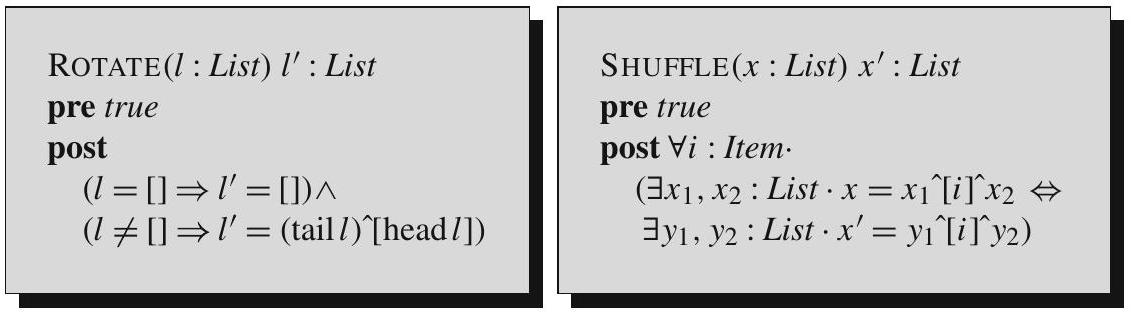
\includegraphics[max width=\textwidth, center]{2025_05_12_af19cd5e0d1b8a465ffeg-068}

Here """ stands for the concatenation of lists, and "•" separates quantifiers with their variables from the rest of the formula. The functions "head $l$ " and "tail $l$ " choose the first element and the rest from the list, respectively. The specification of shuffle indicates that every list element $i$ that was in the list ( $x$ ) before the application of shuffle must be in the result $\left(x^{\prime}\right)$ after the application, and vice versa. It must now be shown that the formula $\left(P R E_{Q} \Rightarrow P R E_{M}\right) \wedge\left(P O S T_{M} \Rightarrow P O S T_{Q}\right)$ is a consequence of the knowledge base containing a description of the data type List. The two VDM-SL specifications yield the proof task

$$
\begin{aligned}
& \forall l, l^{\prime}, x, x^{\prime}: \text { List } \cdot\left(l=x \wedge l^{\prime}=x^{\prime} \wedge(w \Rightarrow w)\right) \wedge \\
& \quad\left(l=x \wedge l^{\prime}=x^{\prime} \wedge\left(\left(l=[] \Rightarrow l^{\prime}=[]\right) \wedge\left(l \neq[] \Rightarrow l^{\prime}=(\text { tll })^{\wedge}[\text { hdl }]\right)\right.\right. \\
& \left.\left.\quad \Rightarrow \forall i: \text { Item } \cdot\left(\exists x_{1}, x_{2}: \text { List } \cdot x=x_{1} \uparrow[i]^{\wedge} x_{2} \Leftrightarrow \exists y_{1}, y_{2}: \text { List } \cdot x^{\prime}=y_{1} \uparrow[i]^{\wedge} y_{2}\right)\right)\right)
\end{aligned}
$$

which can then be proven with the prover SETHEO.\\
In the coming years the semantic web will likely represent an important application of PL1. The content of the World Wide Web is supposed to become interpretable not only for people, but for machines. To this end web sites are being furnished with a description of their semantics in a formal description language. The search for information in the web will thereby become significantly more effective than today, where essentially only text building blocks are searchable.

Decidable subsets of predicate logic are used as description languages. The development of efficient calculi for reasoning is very important and closely connected to the description languages. A query for a future semantically operating search engine could (informally) read: Where in Switzerland next Sunday at elevations under 2000 meters will there be good weather and optimally prepared ski slopes? To answer such a question, a calculus is required that is capable of working very quickly on large sets of facts and rules. Here, complex nested function terms are less important.

As a basic description framework, the World Wide Web Consortium developed the language RDF (Resource Description Framework). Building on RDF, the significantly more powerful language OWL (Web Ontology Language) allows the description of relations between objects and classes of objects, similarly to PL1 [SET09]. Ontologies are descriptions of relationships between possible objects.

A difficulty when building a description of the innumerable websites is the expenditure of work and also checking the correctness of the semantic descriptions. Here machine learning systems for the automatic generation of descriptions can be very helpful. An interesting use of "automatic" generation of semantics in the web was introduced by Luis von Ahn of Carnegie Mellon University [vA06]. He developed computer games in which the players, distributed over the network, are supposed to collaboratively describe pictures with key words. Thus the pictures are assigned semantics in a fun way at no cost.

\subsection*{3.9 Summary}
We have provided the most important foundations, terms, and procedures of predicate logic and we have shown that even one of the most difficult intellectual tasks, namely the proof of mathematical theorems, can be automated. Automated provers can be employed not only in mathematics, but rather, in particular, in verification tasks in computer science. For everyday reasoning, however, predicate logic in most cases is ill-suited. In the next and the following chapters we show its weak points and some interesting modern alternatives. Furthermore, we will show in Chap. 5 that one can program elegantly with logic and its procedural extensions.

Anyone interested in first-order logic, resolution and other calculi for automated provers will find good advanced instruction in [New00, Fit96, Bib82, Lov78, CL73]. References to Internet resources can be found on this book's web site.

\subsection*{3.10 Exercises}
Exercise 3.1 Let the three-place predicate "child" and the one-place predicate "female" from Example 3.2 on page 43 be given. Define:\\
(a) A one-place predicate "male".\\
(b) A two-place predicate "father" and "mother".\\
(c) A two-place predicate "siblings".\\
(d) A predicate "parents $(x, y, z)$ ", which is true if and only if $x$ is the father and $y$ is the mother of $z$.\\
(e) A predicate "uncle $(x, y)$ ", which is true if and only if $x$ is the uncle of $y$ (use the predicates that have already been defined).\\
(f) A two-place predicate "ancestor" with the meaning: ancestors are parents, grandparents, etc. of arbitrarily many generations.

Exercise 3.2 Formalize the following statements in predicate logic:\\
(a) Every person has a father and a mother.\\
(b) Some people have children.\\
(c) All birds fly.\\
(d) There is an animal that eats (some) grain-eating animals.\\
(e) Every animal eats plants or plant-eating animals which are much smaller than itself.

Exercise 3.3 Adapt Exercise 3.1 on page 63 by using one-place function symbols and equality instead of "father" and "mother".

Exercise 3.4 Give predicate logic axioms for the two-place relation " $<$ " as a total order. For a total order we must have (1) Any two elements are comparable. (2) It is symmetric. (3) It is transitive.

Exercise 3.5 Unify (if possible) the following terms and give the MGU and the resulting terms.\\
(a) $p(x, f(y)), p(f(z), u)$\\
(b) $p(x, f(x)), p(y, y)$\\
(c) $x=4-7 \cdot x, \cos y=z$\\
(d) $x<2 \cdot x, 3<6$\\
(e) $q(f(x, y, z), f(g(w, w), g(x, x), g(y, y))), q(u, u)$

\section*{Exercise 3.6}
(a) Transform Russell's Paradox from Example 3.7 on page 54 into CNF.\\
(b) Show that the empty clause cannot be derived using resolution without factorization from (3.7) on page 54. Try to understand this intuitively.

\section*{Exercise 3.7}
(a) Why is resolution with the set of support strategy incomplete?\\
(b) Justify (without proving) why the set of support strategy becomes complete if $(K B \wedge \neg Q) \backslash S O S$ is satisfiable.\\
(c) Why is resolution with the pure literal rule complete?

\begin{itemize}
  \item Exercise 3.8 Formalize and prove with resolution that in a semigroup with at least two different elements $a, b$, a left-neutral element e , and a left null element n , these two elements have to be different, that is, that $n \neq e$. Use demodulation, which allows replacement of "like with like".
\end{itemize}

Exercise 3.9 Obtain the theorem prover E [Sch02] or another prover and prove the following statements. Compare these proofs with those in the text.\\
(a) The claim from Example 2.3 on page 33.\\
(b) Russell's paradox from Example 3.7 on page 54.\\
(c) The claim from Exercise 3.8.

\section*{Limitations of Logic}
\section*{4}
\subsection*{4.1 The Search Space Problem}
As already mentioned in several places, in the search for a proof there are almost always many (depending on the calculus, potentially infinitely many) possibilities for the application of inference rules at every step. The result is the aforementioned explosive growth of the search space (Fig. 4.1 on page 66). In the worst case, all of these possibilities must be tried in order to find the proof, which is usually not possible in a reasonable amount of time.

If we compare automated provers or inference systems with mathematicians or human experts who have experience in special domains, we make interesting observations. For one thing, experienced mathematicians can prove theorems which are far out of reach for automated provers. On the other hand, automated provers perform tens of thousands of inferences per second. A human in contrast performs maybe one inference per second. Although human experts are much slower on the object level (that is, in carrying out inferences), they apparently solve difficult problems much faster.

There are several reasons for this. We humans use intuitive calculi that work on a higher level and often carry out many of the simple inferences of an automated prover in one step. Furthermore, we use lemmas, that is, derived true formulas that we already know and therefore do not need to re-prove them each time. Meanwhile there are also machine provers that work with such methods. But even they cannot yet compete with human experts.

A further, much more important advantage of us humans is intuition, without which we could not solve any difficult problems [PS09]. The attempt to formalize intuition causes problems. Experience in applied AI projects shows that in complex domains such as medicine (see Sect. 7.3) or mathematics, most experts are unable to formulate this intuitive meta-knowledge verbally, much less to formalize it. Therefore we cannot program this knowledge or integrate it into calculi in the form of heuristics. Heuristics are methods that in many cases can greatly simplify or shorten the way to the goal, but in some cases (usually rarely) can greatly lengthen\\
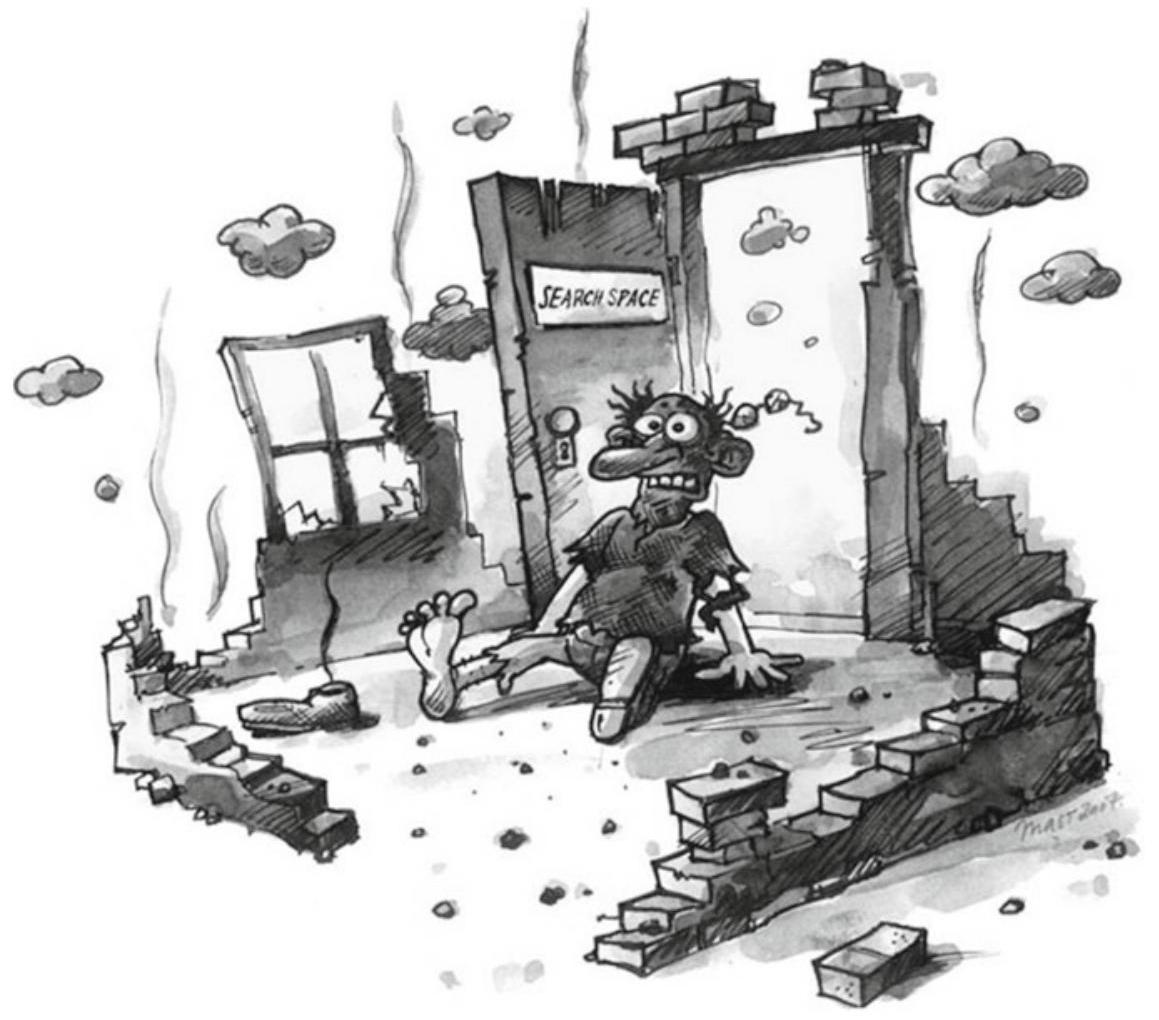
\includegraphics[max width=\textwidth, center]{2025_05_12_af19cd5e0d1b8a465ffeg-072}

Fig. 4.1 Possible consequences of the explosion of a search space\\
the way to the goal. Heuristic search is important not only to logic, but generally to problem solving in AI and will therefore be thoroughly handled in Chap. 6.

An interesting approach, which has been pursued since about 1990, is the application of machine learning techniques to the learning of heuristics for directing the search of inference systems, which we will briefly sketch now. A resolution prover has, during the search for a proof, hundreds or more possibilities for resolution steps at each step, but only a few lead to the goal. It would be ideal if the prover could ask an oracle which two clauses it should use in the next step to quickly find the proof. There are attempts to build such proof-directing modules, which evaluate the various alternatives for the next step and then choose the alternative with the best rating. In the case of resolution, the rating of the available clauses could be computed by a function that calculates a value based on the number of positive literals, the complexity of the terms, etc., for every pair of resolvable clauses.

How can this function be implemented? Because this knowledge is "intuitive", the programmer is not familiar with it. Instead, one tries to copy nature and uses machine learning algorithms to learn from successful proofs [ESS89, SE90].

The attributes of all clause pairs participating in successful resolution steps are stored as positive, and the attributes of all unsuccessful resolutions are stored as negative. Then, using this training data and a machine learning system, a program is generated which can rate clause pairs heuristically (see Sect. 9.5).

A different, more successful approach to improving mathematical reasoning is followed with interactive systems that operate under the control of the user. Here one could name computer algebra programs such as Mathematica, Maple, or Maxima, which can automatically carry out difficult symbolic mathematical manipulations. The search for the proof, however, is left fully to the human. The aforementioned interactive prover Isabelle [NPW02] provides distinctly more support during the proof search. There are at present several projects, such as Omega [SB04] and MKM, ${ }^{1}$ for the development of systems for supporting mathematicians during proofs.

In summary, one can say that, because of the search space problem, automated provers today can only prove relatively simple theorems in special domains with few axioms.

\subsection*{4.2 Decidability and Incompleteness}
First-order predicate logic provides a powerful tool for the representation of knowledge and reasoning. We know that there are correct and complete calculi and theorem provers. When proving a theorem, that is, a true statement, such a prover is very helpful because, due to completeness, one knows after finite time that the statement really is true. What if the statement is not true? The completeness theorem (Theorem 3.3 on page 50) does not answer this question. ${ }^{2}$ Specifically, there is no process that can prove or refute any formula from PL1 in finite time, for it holds that

\section*{Theorem 4.1 The set of valid formulas in first-order predicate logic is semidecidable.}
This theorem implies that there are programs (theorem provers) which, given a true (valid) formula as input, determine its truth in finite time. If the formula is not valid, however, it may happen that the prover never halts. (The reader may grapple with this question in Exercise 4.1 on page 73.) Propositional logic is decidable because the truth table method provides all models of a formula in finite time. Evidently predicate logic with quantifiers and nested function symbols is a language somewhat too powerful to be decidable.

\footnotetext{${ }^{1}$ \href{http://www.mathweb.org/mathweb/demo.html}{www.mathweb.org/mathweb/demo.html}.\\
${ }^{2}$ Just this case is especially important in practice, because if I already know that a statement is true, I no longer need a prover.
}On the other hand, predicate logic is not powerful enough for many purposes. One often wishes to make statements about sets of predicates or functions. This does not work in PL1 because it only knows quantifiers for variables, but not for predicates or functions.

Kurt Gödel showed, shortly after his completeness theorem for PL1, that completeness is lost if we extend PL1 even minimally to construct a higher-order logic. A first-order logic can only quantify over variables. A second-order logic can also quantify over formulas of the first order, and a third-order logic can quantify over formulas of the second order. Even adding only the induction axiom for the natural numbers makes the logic incomplete. The statement "If a predicate $p(n)$ holds for $n$, then $p(n+1)$ also holds", or

$$
\forall p p(n) \Rightarrow p(n+1)
$$

is a second-order proposition because it quantifies over a predicate. Gödel proved the following theorem:

Theorem 4.2 (Gödel's incompleteness theorem) Every axiom system for the natural numbers with addition and multiplication (arithmetic) is incomplete. That is, there are true statements in arithmetic that are not provable.

Gödel's proof works with what is called Gödelization, in which every arithmetic formula is encoded as a number. It obtains a unique Gödel number. Gödelization is now used to formulate the proposition

$$
F=\text { "I am not provable." }
$$

in the language of arithmetic. This formula is true for the following reason. Assume $F$ is false. Then we can prove $F$ and therefore show that $F$ is not provable. This is a contradiction. Thus $F$ is true and therefore not provable.

The deeper background of this theorem is that mathematical theories (axiom systems) and, more generally, languages become incomplete if the language becomes too powerful. A similar example is set theory. This language is so powerful that one can formulate paradoxes with it. These are statements that contradict themselves, such as the statement we already know from Example 3.7 on page 54 about the barbers who all shave those who do not shave themselves (see Exercise 4.2 on page 73). The dilemma consists therein that with languages which are powerful enough to describe mathematics and interesting applications, we are smuggling contradictions and incompletenesses through the back door. This does not mean, however, that higher-order logics are wholly unsuited for formal methods. There are certainly formal systems as well as provers for higher-order logics.

\subsection*{4.3 The Flying Penguin}
With a simple example we will demonstrate a fundamental problem of logic and possible solution approaches. Given the statements

\begin{enumerate}
  \item Tweety is a penguin
  \item Penguins are birds
  \item Birds can fly
\end{enumerate}

Formalized in PL1, the knowledge base $K B$ results:

$$
\begin{aligned}
& \text { penguin(tweety) } \\
& \text { penguin }(x) \Rightarrow \operatorname{bird}(x) \\
& \operatorname{bird}(x) \Rightarrow \operatorname{fly}(x)
\end{aligned}
$$

From there (for example with resolution) fly(tweety) can be derived (Fig. 4.2 on page 70). ${ }^{3}$ Evidently the formalization of the flight attributes of penguins is insufficient. We try the additional statement Penguins cannot fly, that is

$$
\operatorname{penguin}(x) \Rightarrow \neg f l y(x)
$$

From there $\neg$ fly(tweety) can be derived. But fly(tweety) is still true. The knowledge base is therefore inconsistent. Here we notice an important characteristic of logic, namely monotony. Although we explicitly state that penguins cannot fly, the opposite can still be derived.

Definition 4.1 A logic is called monotonic if, for an arbitrary knowledge base $K B$ and an arbitrary formula $\phi$, the set of formulas derivable from $K B$ is a subset of the formulas derivable from $K B \cup \phi$.

If a set of formulas is extended, then, after the extension, all previously derivable statements can still be proved, and additional statements can potentially also be proved. The set of provable statements thus grows monotonically when the set of formulas is extended. For our example this means that the extension of the knowledge base will never lead to our goal. We thus modify $K B$ by replacing the obviously false statement "(all) birds can fly" with the more exact statement "(all) birds except penguins can fly" and obtain as $\mathrm{KB}_{2}$ the following clauses:

$$
\begin{aligned}
& \text { penguin(tweety) } \\
& \text { penguin }(x) \Rightarrow \operatorname{bird}(x) \\
& \operatorname{bird}(x) \wedge \neg \operatorname{penguin}(x) \Rightarrow f l y(x) \\
& \operatorname{penguin}(x) \Rightarrow \neg f l y(x)
\end{aligned}
$$

\footnotetext{${ }^{3}$ The formal execution of this and the following simple proof may be left to the reader (Exercise 4.3 on page 73).
}
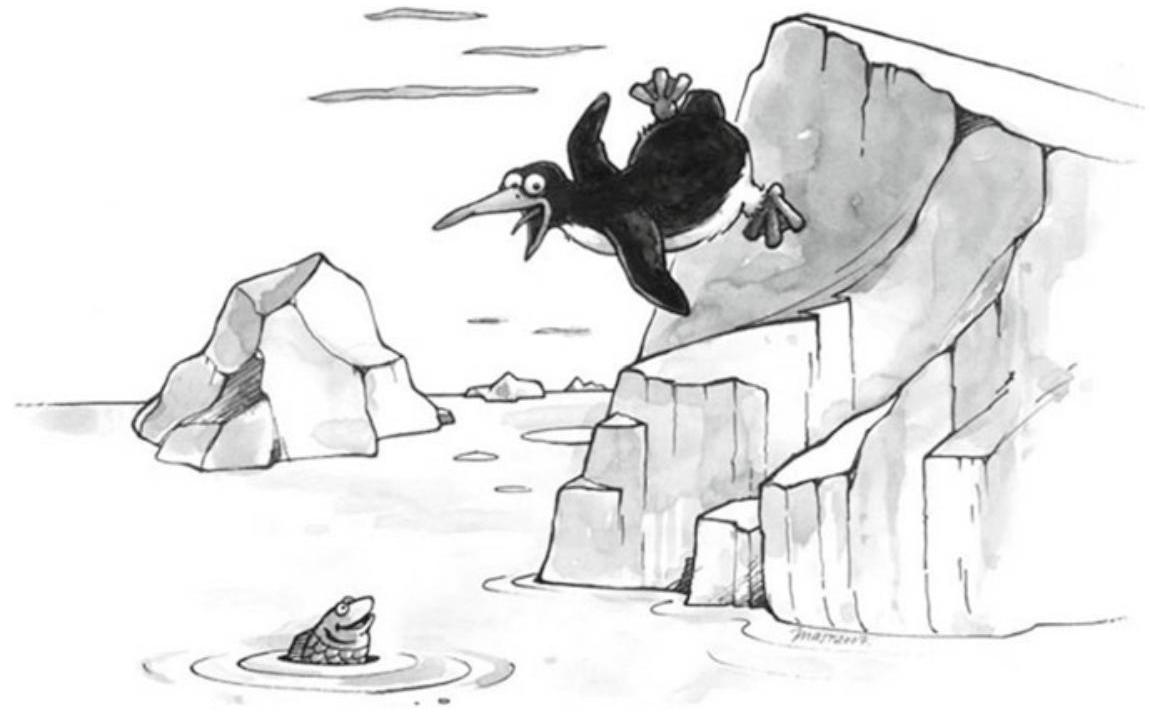
\includegraphics[max width=\textwidth, center]{2025_05_12_af19cd5e0d1b8a465ffeg-076}

Fig. 4.2 The flying penguin Tweety

Now the world is apparently in order again. We can derive $\neg$ fly(tweety), but not fly (tweety), because for that we would need $\neg$ penguin $(x)$, which, however, is not derivable. As long as there are only penguins in this world, peace reigns. Every normal bird, however, immediately causes problems. We wish to add the raven Abraxas (from the German book "The Little Witch") and obtain

$$
\begin{aligned}
& \operatorname{raven}(\text { abraxas }) \\
& \operatorname{raven}(x) \Rightarrow \operatorname{bird}(x) \\
& \text { penguin }(\text { tweety }) \\
& \operatorname{penguin}(x) \Rightarrow \operatorname{bird}(x) \\
& \operatorname{bird}(x) \wedge \neg \operatorname{penguin}(x) \Rightarrow \operatorname{fly}(x) \\
& \operatorname{penguin}(x) \Rightarrow \neg \operatorname{fly}(x)
\end{aligned}
$$

We cannot say anything about the flight attributes of Abraxas because we forgot to formulate that ravens are not penguins. Thus we extend $K B_{3}$ to $K B_{4}$ :

$$
\begin{aligned}
& \operatorname{raven}(\text { abraxas }) \\
& \operatorname{raven}(x) \Rightarrow \operatorname{bird}(x) \\
& \operatorname{raven}(x) \Rightarrow \neg \operatorname{pinguin}(x) \\
& \operatorname{penguin}(\text { tweety }) \\
& \operatorname{penguin}(x) \Rightarrow \operatorname{bird}(x) \\
& \operatorname{bird}(x) \wedge \neg \operatorname{penguin}(x) \Rightarrow \operatorname{fly}(x) \\
& \operatorname{penguin}(x) \Rightarrow \neg \operatorname{fly}(x)
\end{aligned}
$$

The fact that ravens are not penguins, which is self-evident to humans, must be explicitly added here. For the construction of a knowledge base with all 9,800 or so\\
types of birds worldwide, it must therefore be specified for every type of bird (except for penguins) that it is not a member of penguins. We must proceed analogously for all other exceptions such as the ostrich.

For every object in the knowledge base, in addition to its attributes, all of the attributes it does not have must be listed.

To solve this problem, various forms of non-monotonic logic have been developed, which allow knowledge (formulas) to be removed from the knowledge base. Under the name default logic, logics have been developed which allow objects to be assigned attributes which are valid as long as no other rules are available. In the Tweety example, the rule birds can fly would be such a default rule. Despite great effort, these logics have at present, due to semantic and practical problems, not succeeded.

Monotony can be especially inconvenient in complex planning problems in which the world can change. If for example a blue house is painted red, then afterwards it is red. A knowledge base such as

$$
\begin{aligned}
& \text { color }(\text { house }, \text { blue }) \\
& \text { paint }(\text { house }, \text { red }) \\
& \text { paint }(x, y) \Rightarrow \operatorname{color}(x, y)
\end{aligned}
$$

leads to the conclusion that, after painting, the house is red and blue. The problem that comes up here in planning is known as the frame problem. A solution for this is the situation calculus presented in Sect. 5.6.

An interesting approach for modeling problems such as the Tweety example is probability theory. The statement "all birds can fly" is false. A statement something like "almost all birds can fly" is correct. This statement becomes more exact if we give a probability for "birds can fly". This leads to probabilistic logic, which today represents an important sub-area of AI and an important tool for modeling uncertainty (see Chap. 7).

\subsection*{4.4 Modeling Uncertainty}
Two-valued logic can and should only model circumstances in which there is true, false, and no other truth values. For many tasks in everyday reasoning, two-valued logic is therefore not expressive enough. The rule

$$
\operatorname{bird}(x) \Rightarrow f l y(x)
$$

is true for almost all birds, but for some it is false. As was already mentioned, working with probabilities allows exact formulation of uncertainty. The statement "99\% of all birds can fly" can be formalized by the expression

$$
P(\operatorname{bird}(x) \Rightarrow f l y(x))=0.99
$$

\begin{center}
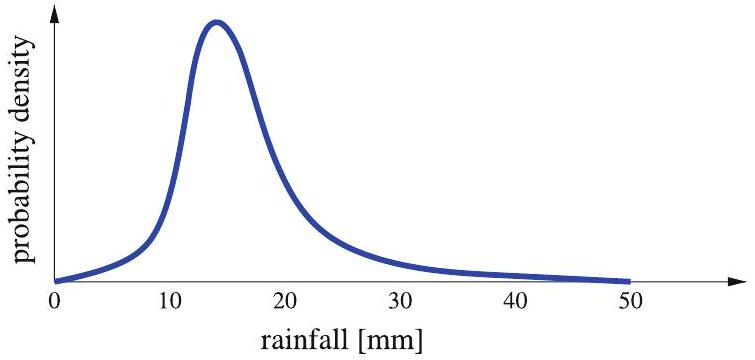
\includegraphics[max width=\textwidth]{2025_05_12_af19cd5e0d1b8a465ffeg-078}
\end{center}

Fig. 4.3 Probability density of the continuous variable rainfall

In Chap. 7 we will see that here it is better to work with conditional probabilities such as

$$
P(\text { fly } \mid \text { bird })=0.99 .
$$

With the help of Bayesian networks, complex applications with many variables can also be modeled.

A different model is needed for the statement "The weather is nice". Here it often makes no sense to speak in terms of true and false. The variable weather\_is\_nice should not be modeled as binary, rather continuously with values, for example, in the interval $[0,1]$. weather\_is\_nice $=0.7$ then means "The weather is fairly nice". Fuzzy logic was developed for this type of continuous (fuzzy) variable.

Probability theory also offers the possibility of making statements about the probability of continuous variables. A statement in the weather report such as "There is a high probability that there will be some rain" could for example be exactly formulated as a probability density of the form

$$
P(\text { rainfall }=X)=Y
$$

and represented graphically something like in Fig. 4.3.\\
This very general and even visualizable representation of both types of uncertainty we have discussed, together with inductive statistics and the theory of Bayesian networks, makes it possible, in principle, to answer arbitrary probabilistic queries.

Probability theory as well as fuzzy logic are not directly comparable to predicate logic because they do not allow variables or quantifiers. They can thus be seen as extensions of propositional logic as shown in the following table.

\begin{center}
\begin{tabular}{|l|l|l|}
\hline
Formalism & Number of truth values & Probabilities expressible \\
\hline
Propositional logic & 2 & - \\
\hline
Fuzzy logic & $\infty$ & - \\
\hline
Discrete probabilistic logic & $n$ & yes \\
\hline
Continuous probabilistic logic & $\infty$ & yes \\
\hline
\end{tabular}
\end{center}

\subsection*{4.5 Exercises}
\section*{薔 Exercise 4.1}
(a) With the following (false) argument, one could claim that PL1 is decidable: We take a complete proof calculus for PL1. With it we can find a prooffor any true formula in finite time. For every other formula $\phi$ I proceed as follows: I apply the calculus to $\neg \phi$ and show that $\neg \phi$ is true. Thus $\phi$ is false. Thus I can prove or refute every formula in PL1. Find the mistake in the argument and change it so it becomes correct.\\
(b) Construct a decision process for the set of true and unsatisfiable formulas in PL1.

\section*{Exercise 4.2}
(a) Given the statement "There is a barber who shaves every person who does not shave himself." Consider whether this barber shaves himself.\\
(b) Let $M=\{x \mid x \notin x\}$. Describe this set and consider whether $M$ contains itself.

Exercise 4.3 Use an automated theorem prover (for example E [Sch02]) and apply it to all five different axiomatizations of the Tweety example from Sect. 4.3. Validate the example's statements.

\section*{Logic Programming with PROLOG}
\section*{5}
Compared to classical programming languages such as C or Pascal, Logic makes it possible to express relationships elegantly, compactly, and declaratively. Automated theorem provers are even capable of deciding whether a knowledge base logically entails a query. Proof calculus and knowledge stored in the knowledge base are strictly separated. A formula described in clause normal form can be used as input data for any theorem prover, independent of the proof calculus used. This is of great value for reasoning and the representation of knowledge.

If one wishes to implement algorithms, which inevitably have procedural components, a purely declarative description is often insufficient. Robert Kowalski, one of the pioneers of logic programming, made this point with the formula

$$
\text { Algorithm }=\text { Logic }+ \text { Control } .
$$

This idea was brought to fruition in the language PROLOG. PROLOG is used in many projects, primarily in AI and computational linguistics. We will now give a short introduction to this language, present the most important concepts, show its strengths, and compare it with other programming languages and theorem provers. Those looking for a complete programming course are directed to textbooks such as [Bra11, CM94] and the handbooks [Wie04, Dia04].

The syntax of the language PROLOG only allows Horn clauses. Logical notation and PROLOG's syntax are juxtaposed in the following table:

\begin{center}
\begin{tabular}{lll}
\hline
PL1 / clause normal form & PROLOG & Description \\
\hline
$\left(\neg A_{1} \vee \ldots \vee \neg A_{m} \vee B\right)$ & $\mathrm{B}:-\mathrm{A}_{1}, \ldots, \mathrm{~A}_{\mathrm{m}}$. & Rule \\
\hline
$\left(A_{1} \wedge \ldots \wedge A_{m}\right) \Rightarrow B$ & $\mathrm{~B}:-\mathrm{A}_{1}, \ldots, \mathrm{~A}_{\mathrm{m}}$. & Rule \\
\hline
$A$ & A. & Fact \\
\hline
$\left(\neg A_{1} \vee \ldots \vee \neg A_{m}\right)$ & $?-\mathrm{A}_{1}, \ldots, \mathrm{~A}_{\mathrm{m}}$. & Query \\
\hline
$\neg\left(A_{1} \wedge \ldots \wedge A_{m}\right)$ & $?-\mathrm{A}_{1}, \ldots, \mathrm{~A}_{\mathrm{m}}$. & Query \\
\hline
\end{tabular}
\end{center}

Here $A_{1}, \ldots, A_{m}, A, B$ are literals. The literals are, as in PL1, constructed from predicate symbols with terms as arguments. As we can see in the above table, in PROLOG there are no negations in the strict logical sense because the sign of a literal is determined by its position in the clause.

\subsection*{5.1 PROLOG Systems and Implementations}
An overview of current PROLOG systems is available in the collection of links on this book's home page. To the reader we recommend the very powerful and freely available (under GNU public licenses) systems GNU-PROLOG [Dia04] and SWI-PROLOG. For the following examples, SWI-PROLOG [Wie04] was used.

Most modern PROLOG systems work with an interpreter based on the Warren abstract machine (WAM). PROLOG source code is compiled into so-called WAM code, which is then interpreted by the WAM. The fastest implementations of a WAM manage up to 10 million logical inferences per second (LIPS) on a 1 GHz PC .

\subsection*{5.2 Simple Examples}
We begin with the family relationships from Example 3.2 on page 43. The small knowledge base $K B$ is coded-without the facts for the predicate female-as a PROLOG program named \href{http://rel.pl}{rel.pl} in Fig. 5.1.

The program can be loaded and compiled in the PROLOG interpreter with the command

\begin{verbatim}
?- [rel].
\end{verbatim}

\begin{verbatim}
child(oscar,karen,frank).
child(mary,karen,frank).
child(eve,anne,oscar).
child(henry,anne,oscar).
child(isolde,anne,oscar).
child(clyde,mary,oscarb).
child(X,Z,Y) :- child(X,Y,Z).
descendant(X,Y) :- child(X,Y,Z).
descendant(X,Y) :- child(X,U,V), descendant(U,Y).
\end{verbatim}

Fig. 5.1 PROLOG program with family relationships

An initial query returns the dialog\\
?- child(eve,oscar, anne).

Yes\\
with the correct answer Yes. How does this answer come about? For the query "? - child (eve, oscar, anne) ." there are six facts and one rule with the same predicate in its clause head. Now unification is attempted between the query and each of the complementary literals in the input data in order of occurrence. If one of the alternatives fails, this results in backtracking to the last branching point, and the next alternative is tested. Because unification fails with every fact, the query is unified with the recursive rule in line 8 . Now the system attempts to solve the subgoal child (eve, anne, oscar), which succeeds with the third alternative. The query\\
?- descendant (X,Y).

X = oscar\\
Y = karen

Yes\\
is answered with the first solution found, as is\\
?- descendant (clyde,Y).\\
$\mathrm{Y}=\mathrm{mar} \mathrm{y}$

Yes\\
The query\\
?- descendant (clyde, karen).\\
is not answered, however. The reason for this is the clause in line 8 , which specifies symmetry of the child predicate. This clause calls itself recursively without the possibility of termination. This problem can be solved with the following new program (facts have been omitted here).

\begin{verbatim}
descendant(X,Y) :- child(X,Y,Z).
descendant(X,Y) :- child(X,Z,Y).
descendant(X,Y) :- child(X,U,V), descendant(U,Y).
\end{verbatim}

But now the query\\
?- child(eve,oscar, anne).\\
is no longer correctly answered because the symmetry of child in the last two variables is no longer given. A solution to both problems is found in the program

\begin{verbatim}
child_fact(oscar,karen,franz).
child_fact(mary, karen, franz).
child_fact(eva,anne,oscar).
child_fact(henry,anne,oscar).
child_fact(isolde,anne,oscar).
child_fact(clyde,mary,oscarb).
child(X,Z,Y) :- child_fact(X,Y,Z).
child(X,Z,Y) :- child_fact(X,Z,Y).
descendant(X,Y) :- child(X,Y,Z).
descendant(X,Y) :- child(X,U,V), descendant(U,Y).
\end{verbatim}

By introducing the new predicate child\_fact for the facts, the predicate child is no longer recursive. However, the program is no longer as elegant and simple as the-logically correct-first variant in Fig. 5.1 on page 76, which leads to the infinite loop. The PROLOG programmer must, just as in other languages, pay attention to processing and avoid infinite loops. PROLOG is just a programming language and not a theorem prover.

We must distinguish here between declarative and procedural semantics of PROLOG programs. The declarative semantics is given by the logical interpretation of the horn clauses. The procedural semantics, in contrast, is defined by the execution of the PROLOG program, which we wish to observe in more detail now. The execution of the program from Fig. 5.1 on page 76 with the query child (eve, oscar, anne) is represented in Fig. 5.2 as a search tree. ${ }^{1}$ Execution begins at the top left with the query. Each edge represents a possible SLD resolution step with a complementary unifiable literal. While the search tree becomes infinitely deep by the recursive rule, the PROLOG execution terminates because the facts occur before the rule in the input data.\\
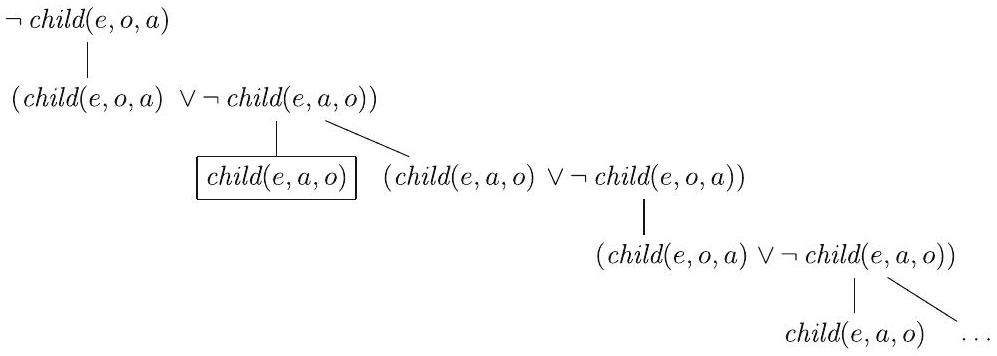
\includegraphics[max width=\textwidth, center]{2025_05_12_af19cd5e0d1b8a465ffeg-083}

Fig. 5.2 PROLOG search tree for child (eve, oscar, anne)

\footnotetext{${ }^{1}$ The constants have been abbreviated to save space.
}
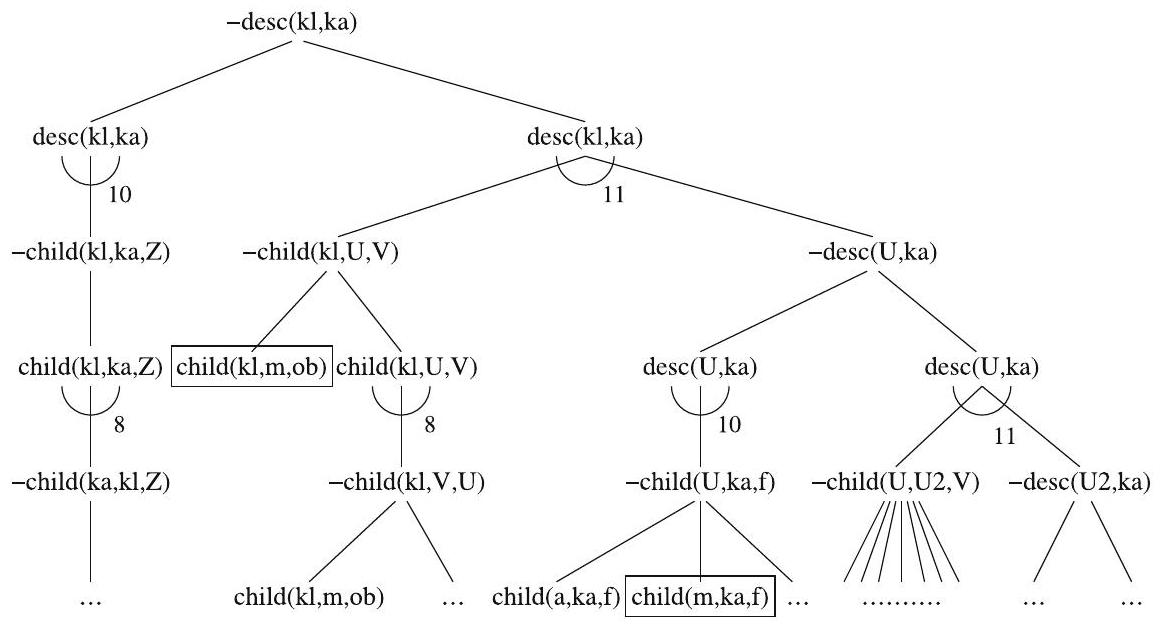
\includegraphics[max width=\textwidth, center]{2025_05_12_af19cd5e0d1b8a465ffeg-084}

Fig. 5.3 And-or tree for desc (clyde, karen)\\
With the query descendant (clyde, karen), in contrast, the PROLOG execution does not terminate. We can see this clearly in the and-or tree presented in Fig. 5.3. In this representation the branches, represented by , lead from the head of a clause to the subgoals. Because all subgoals of a clause must be solved, these are and branches. All other branches are or branches, of which at least one must be unifiable with its parent nodes. The two outlined facts represent the solution to the query. The PROLOG interpreter does not terminate here, however, because it works by using a depth-first search with backtracking (see Sect. 6.2.2) and thus first chooses the infinitely deep path to the far left.

\subsection*{5.3 Execution Control and Procedural Elements}
As we have seen in the family relationship example, it is important to control the execution of PROLOG. Avoiding unnecessary backtracking especially can lead to large increases in efficiency. One means to this end is the cut. By inserting an exclamation mark into a clause, we can prevent backtracking over this point. In the following program, the predicate max ( $\mathrm{X}, \mathrm{Y}, \operatorname{Max}$ ) computes the maximum of the two numbers X and Y .

\begin{verbatim}
1 max(X,Y,X) :- X >= Y.
2 max(X,Y,Y) :- X < Y.
\end{verbatim}

If the first case (first clause) applies, then the second will not be reached. On the other hand, if the first case does not apply, then the condition of the second case is true, which means that it does not need to be checked. For example, in the query\\
?- max(3,2,Z), Z > 10.\\
backtracking is employed because $\mathrm{Z}=3$, and the second clause is tested for max, which is doomed to failure. Thus backtracking over this spot is unnecessary. We can optimize this with a cut:

\begin{verbatim}
1 max(X,Y,X) :- X >= Y, !.
2 max(X,Y,Y).
\end{verbatim}

Thus the second clause is only called if it is really necessary, that is, if the first clause fails. However, this optimization makes the program harder to understand.

Another possibility for execution control is the built-in predicate fail, which is never true. In the family relationship example we can quite simply print out all children and their parents with the query

\begin{verbatim}
?- child\_fact(X,Y,Z), write(X), write(' is a child of '),
write(Y), write(' and '), write(Z), write('.'), nl, fail.
\end{verbatim}

The corresponding output is

\begin{verbatim}
oscar is a child of karen and frank.
mary is a child of karen and frank.
eve is a child of anne and oscar.
No.
\end{verbatim}

where the predicate nl causes a line break in the output. What would be the output in the end without use of the fail predicate?

With the same knowledge base, the query "?- child\_fact (ulla, X, Y)." would result in the answer No because there are no facts about ulla. This answer is not logically correct. Specifically, it is not possible to prove that there is no object with the name ulla. Here the prover E would correctly answer "No proof found." Thus if PROLOG answers No, this only means that the query $Q$ cannot be proved. For this, however, $\neg Q$ must not necessarily be proved. This behavior is called negation as failure.

Restricting ourselves to Horn clauses does not cause a big problem in most cases. However, it is important for procedural execution using SLD-resolution (Sect. 2.5). Through the singly determined positive literal per clause, SLD resolution, and therefore the execution of PROLOG programs, have a unique entry point into the clause. This is the only way it is possible to have reproducible execution of logic programs and, therefore, well-defined procedural semantics.

Indeed, there are certainly problem statements which cannot be described by Horn clauses. An example is Russell's paradox from Example 3.7 on page 54, which contains the non-Horn clause (shaves(barber, $X$ ) $\vee$ shaves $(X, X)$ ).

\subsection*{5.4 Lists}
As a high-level language, PROLOG has, like the language LISP, the convenient generic list data type. A list with the elements $A, 2,2, B, 3,4,5$ has the form\\[0pt]
[A, 2, 2, B, 3, 4, 5]\\[0pt]
The construct [Head|Tail] separates the first element (Head) from the rest (Tail) of the list. With the knowledge base\\[0pt]
list ([A,2,2,B,3,4,5]).\\
PROLOG displays the dialog\\[0pt]
?- list([H|T]).\\
$\mathrm{H}=\mathrm{A}$\\
$T=[2,2, B, 3,4,5]$

Yes\\
By using nested lists, we can create arbitrary tree structures. For example, the two trees\\
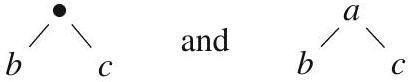
\includegraphics[max width=\textwidth, center]{2025_05_12_af19cd5e0d1b8a465ffeg-086}\\
can be represented by the lists $[\mathrm{b}, \mathrm{c}]$ and $[\mathrm{a}, \mathrm{b}, \mathrm{c}]$, respectively, and the two trees\\
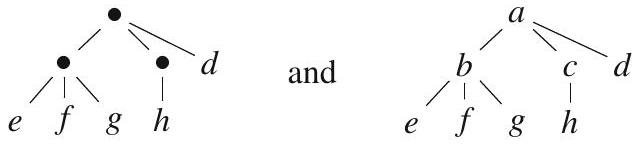
\includegraphics[max width=\textwidth, center]{2025_05_12_af19cd5e0d1b8a465ffeg-086(1)}\\
by the lists $[[e, f, g],[h], d]$ and $[a,[b, e, f, g],[c, h], d]$, respectively. In the trees where the inner nodes contain symbols, the symbol is the head of the list and the child nodes are the tail.

A nice, elegant example of list processing is the definition of the predicate append $(X, Y, Z)$ for appending list $Y$ to the list $X$. The result is saved in $Z$. The corresponding PROLOG program reads

\begin{verbatim}
1 append([],L,L).
2 append([X|L1],L2,[X|L3]) :- append(L1,L2,L3).
\end{verbatim}

This is a declarative (recursive) logical description of the fact that L3 results from appending L2 to L1. At the same time, however, this program also does the work when it is called. The call\\[0pt]
?- append([a,b,c],[d,1,2],z).\\
returns the substitution $Z=[a, b, c, d, 1,2]$, just as the call\\[0pt]
?- append(X, [1,2,3], [4,5,6,1,2,3]).\\
yields the substitution $X=[4,5,6]$. Here we observe that append is not a two-place function, but a three-place relationship. Actually, we can also input the "output parameter" Z and ask whether it can be created.

Reversing the order of a list's elements can also be elegantly described and simultaneously programmed by the recursive predicate

\begin{verbatim}
1 nrev([],[]).
2 nrev([H|T],R) :- nrev(T,RT), append(RT,[H],R).
\end{verbatim}

which reduces the reversal of a list down to the reversal of a list that is one element smaller. Indeed, this predicate is very inefficient due to calling append. This program is known as naive reverse and is often used as a PROLOG benchmark (see Exercise 5.6 on page 89). Things go better when one proceeds using a temporary store, known as the accumulator, as follows:

\begin{center}
\begin{tabular}{ll}
\hline
List & Accumulator \\
\hline
$[\mathrm{a}, \mathrm{b}, \mathrm{c}, \mathrm{d}]$ & [] \\
\hline
$[\mathrm{b}, \mathrm{c}, \mathrm{d}]$ & $[\mathrm{a}]$ \\
\hline
$[\mathrm{c}, \mathrm{d}]$ & $[\mathrm{b}, \mathrm{a}]$ \\
\hline
$[\mathrm{d}]$ & $[\mathrm{c}, \mathrm{b}, \mathrm{a}]$ \\
\hline
[] & $[\mathrm{d}, \mathrm{c}, \mathrm{b}, \mathrm{a}]$ \\
\hline
\end{tabular}
\end{center}

The corresponding PROLOG program reads

\begin{verbatim}
1 accrev([],A,A).
2 accrev([H|T],A,R) :- accrev(T,[H|A],R).
\end{verbatim}

\subsection*{5.5 Self-modifying Programs}
PROLOG programs are not fully compiled, rather, they are interpreted by the WAM. Therefore it is possible to modify programs at runtime. A program can even modify itself. With commands such as assert and retract, facts and rules can be added to the knowledge base or taken out of it.

A simple application of the variant asserta is the addition of derived facts to the beginning of the knowledge base with the goal of avoiding a repeated, potentially time-expensive derivation (see Exercise 5.8 on page 89). If in our family relationship example we replace the two rules for the predicate descendant with

\begin{verbatim}
:- dynamic descendant/2.
descendant(X,Y) :- child(X,Y,Z), asserta(descendant(X,Y)).
descendant(X,Y) :- child(X,U,V), descendant(U,Y),
    asserta(descendant(X,Y)).
\end{verbatim}

then all derived facts for this predicate are saved in the knowledge base and thus in the future are not re-derived. The query

\begin{verbatim}
?- descendant(clyde, karen).
\end{verbatim}

leads to the addition of the two facts

\begin{verbatim}
descendant(clyde, karen).
descendant(mary, karen).
\end{verbatim}

By manipulating rules with assert and retract, even programs that change themselves completely can be written. This idea became known under the term genetic programming. It allows the construction of arbitrarily flexible learning programs. In practice, however, it turns out that, due to the huge number of senseless possible changes, changing the code by trial and error rarely leads to a performance increase. Systematic changing of rules, on the other hand, makes programming so much more complex that, so far, such programs that extensively modify their own code have not been successful. In Chap. 8 we will show how machine learning has been quite successful. However, only very limited modifications of the program code are being conducted here.

\subsection*{5.6 A Planning Example}
Example 5.1 The following riddle serves as a problem statement for a typical PROLOG program.

A farmer wants to bring a cabbage, a goat, and a wolf across a river, but his boat is so small that he can only take them across one at a time. The farmer thought it over and then said to himself: "If I first bring the wolf to the other side, then the goat will eat the cabbage. If I transport the cabbage first, then the goat will be eaten by the wolf. What should I do?"

This is a planning task which we can quickly solve with a bit of thought. The PROLOG program given in Fig. 5.4 on page 84 is not created quite as fast.

The program works on terms of the form state (Farmer, Wolf, Goat, Cabbage), which describe the current state of the world. The four variables with possible values left, right give the location of the objects. The central

\begin{verbatim}
start :- action(state(left,left,left,left),
            state(right,right,right,right)).
action(Start,Goal):-
        plan(Start,Goal,[Start],Path),
        nl,write('Solution:'),nl,
        write_path(Path).
            write_path(Path), fail. % all solutions output
plan(Start,Goal,Visited,Path):-
    go(Start,Next),
    safe(Next),
    \+ member(Next,Visited), % not(member(...))
    plan(Next,Goal,[Next|Visited],Path).
plan(Goal,Goal,Path,Path).
go(state(X,X,Z,K),state(Y,Y,Z,K)):-across(X,Y). % farmer, wolf
go(state(X,W,X,K),state(Y,W,Y,K)):-across(X,Y). % farmer, goat
go(state(X,W,Z,X),state(Y,W,Z,Y)):-across(X,Y). % farmer, cabbage
go(state(X,W,Z,K),state(Y,W,Z,K)):-across(X,Y). % farmer
across(left,right).
across(right,left).
safe(state(B,W,Z,K)) :- across(W,Z), across(Z,K).
safe(state(B,B,B,K)).
safe(state(B,W,B,B)).
\end{verbatim}

Fig. 5.4 PROLOG program for the farmer-wolf-goat-cabbage problem\\
recursive predicate plan first creates a successor state Next using go, tests its safety with safe, and repeats this recursively until the start and goal states are the same (in program line 15). The states which have already been visited are stored in the third argument of plan. With the built-in predicate member it is tested whether the state Next has already been visited. If yes, it is not attempted.

The definition of the predicate write\_path for the task of outputting the plan found is missing here. It is suggested as an exercise for the reader (Exercise 5.2 on page 88). For initial program tests the literal write\_path (Path) can be replaced with write (Path). For the query "? - start." we get the answer

\begin{verbatim}
Solution:
Farmer and goat from left to right
Farmer from right to left
Farmer and wolf from left to right
Farmer and goat from right to left
Farmer and cabbage from left to right
Farmer from right to left
Farmer and goat from left to right
\end{verbatim}

Yes

For better understanding we describe the definition of plan in logic:

$$
\forall z \operatorname{plan}(z, z) \wedge \forall s \forall z \forall n[g o(s, n) \wedge \operatorname{safe}(n) \wedge \operatorname{plan}(n, z) \Rightarrow \operatorname{plan}(s, z)]
$$

This definition comes out significantly more concise than in PROLOG. There are two reasons for this. For one thing, the output of the discovered plan is unimportant for logic. Furthermore, it is not really necessary to check whether the next state was already visited if unnecessary trips do not bother the farmer. If, however, $\backslash+$ member (...) is left out of the PROLOG program, then there is an infinite loop and PROLOG might not find a schedule even if there is one. The cause of this is PROLOG's backward chaining search strategy, which, according to the depth-first search (Sect. 6.2.2) principle, always works on subgoals one at a time without restricting recursion depth, and is therefore incomplete. This would not happen to a theorem prover with a complete calculus.

As in all planning tasks, the state of the world changes as actions are carried out from one step to the next. This suggests sending the state as a variable to all predicates that depend on the state of the world, such as in the predicate safe. The state transitions occur in the predicate go. This approach is called situation calculus [RN10]. We will become familiar with an interesting extension to learning action sequences in partially observable, non-deterministic worlds in Chap. 10.

Predicate logic and simpler sub-languages for the description and solution of planning tasks play an increasingly important role for intelligent robots. To solve complex tasks, robots often work on symbolic relational descriptions of the world. The classic application for a service robot is recognizing an audible command linguistically and then converting it into a logical formula. Then a planner has the task of finding a plan which eventually reaches a state in which the formula becomes true. Even more interesting is when the robot learns to meet the goals of its trainer by observing them and then use the symbolic planner to achieve the goals [CEP15b]. One very exciting thing about this is that the robot is able to take numerical sensor values such as pixel images and turn them into a symbolic description of situations. This generally very difficult task is known in AI as symbol grounding. Robotics developers have found interesting solutions to this problem for certain tasks [CEP15a].

\subsection*{5.7 Constraint Logic Programming}
The programming of scheduling systems, in which many (sometimes complex) logical and numerical conditions must be fulfilled, can be very expensive and difficult with conventional programming languages. This is precisely where logic could be useful. One simply writes all logical conditions in PL1 and then enters a query. Usually this approach fails miserably. The reason is the penguin problem discussed in Sect. 4.3. The fact penguin (tweety) does ensure that penguin (tweety) is true. However, it does not rule out that raven (tweety) is also true. To rule this out with additional axioms is very inconvenient (Sect. 4.3).

Constraint Logic Programming (CLP), which allows the explicit formulation of constraints for variables, offers an elegant and very efficient mechanism for solving this problem. The interpreter constantly monitors the execution of the program for adherence to all of its constraints. The programmer is fully relieved of the task of controlling the constraints, which in many cases can greatly simplify programming. This is expressed in the following quotation by Eugene C. Freuder from [Fre97]:

\begin{displayquote}
Constraint programming represents one of the closest approaches computer science has yet made to the Holy Grail of programming: the user states the problem, the computer solves it.
\end{displayquote}

Without going into the theory of the constraint satisfaction problem (CSP), we will apply the CLP mechanism of GNU-PROLOG to the following example.

Example 5.2 The secretary of Albert Einstein High School has to come up with a plan for allocating rooms for final exams. He has the following information: the four teachers Mayer, Hoover, Miller and Smith give tests for the subjects German, English, Math, and Physics in the ascendingly numbered rooms 1, 2, 3 and 4. Every teacher gives a test for exactly one subject in exactly one room. Besides that, he knows the following about the teachers and their subjects.

\begin{enumerate}
  \item Mr. Mayer never tests in room 4.
  \item Mr. Miller always tests German.
  \item Mr. Smith and Mr. Miller do not give tests in neighboring rooms.
  \item Mrs. Hoover tests Mathematics.
  \item Physics is always tested in room number 4.
  \item German and English are not tested in room 1.
\end{enumerate}

Who gives a test in which room?\\
A GNU-PROLOG program for solving this problem is given in Fig. 5.5. This program works with the variables Mayer, Hoover, Miller, Smith as well as

\begin{verbatim}
start :-
    fd_domain([Mayer, Hoover, Miller, Smith],1,4),
    fd_all_different([Mayer, Miller, Hoover, Smith]),
    fd_domain([German, English, Math, Physics],1,4),
    fd_all_different([German, English, Math, Physics]),
    fd_labeling([Mayer, Hoover, Miller, Smith]),
    Mayer #\=4, % Mayer not in room 4
    Miller #= German, % Miller tests German
    dist(Miller,Smith) #>= 2, % Distance Miller/Smith >= 2
    Hoover #= Math, % Hoover tests mathematics
    Physics #= 4, % Physics in room 4
    German #\=1, % German not in room 1
    English #\=1, % English not in room 1
    nl,
    write([Mayer, Hoover, Miller, Smith]), nl,
    write([German, English, Math, Physics]), nl.
\end{verbatim}

Fig. 5.5 CLP program for the room scheduling problem

German, English, Math, Physics, which can each take on an integer value from 1 to 4 as the room number (program lines 2 and 5). A binding Mayer = 1 and German $=1$ means that Mr. Mayer gives the German test in room 1. Lines 3 and 6 ensure that the four particular variables take on different values. Line 8 ensures that all variables are assigned a concrete value in the case of a solution. This line is not absolutely necessary here. If there were multiple solutions, however, only intervals would be output. In lines 10 to 16 the constraints are given, and the remaining lines output the room numbers for all teachers and all subjects in a simple format.

The program is loaded into GNU-PROLOG with "['\href{http://raumplan.pl}{raumplan.pl}'] .", and with "start." we obtain the output

\begin{verbatim}
[3,1,2,4]
[2,3,1,4]
\end{verbatim}

Represented somewhat more conveniently, we have the following room schedule:

\begin{center}
\begin{tabular}{lllll}
\hline
Room num. & 1 & 2 & 3 & 4 \\
\hline
Teacher & Hoover & Miller & Mayer & Smith \\
\hline
Subject & Math & German & English & Physics \\
\hline
\end{tabular}
\end{center}

GNU-PROLOG has, like most other CLP languages, a so-called finite domain constraint solver, with which variables can be assigned a finite range of integers. This need not necessarily be an interval as in the example. We can also input a list of values. As an exercise the user is invited, in Exercise 5.9 on page 89, to create a CLP program, for example with GNU-PROLOG, for a not-so-simple logic puzzle. This puzzle, supposedly created by Einstein, can very easily be solved with a CLP system. If we tried using PROLOG without constraints, on the other hand, we could easily grind our teeth out. Anyone who finds an elegant solution with PROLOG or a prover, please let it find its way to the author.

\subsection*{5.8 Summary}
Unification, lists, declarative programming, and the relational view of procedures, in which an argument of a predicate can act as both input and output, allow the development of short, elegant programs for many problems. Many programs would be significantly longer and thus more difficult to understand if written in a procedural language. Furthermore, these language features save the programmer time. Therefore PROLOG is also an interesting tool for rapid prototyping, particularly for AI applications. The CLP extension of PROLOG is helpful not only for logic puzzles, but also for many optimization and scheduling tasks.

Since its invention in 1972, in Europe PROLOG has developed into one of Europe's leading programming languages in AI, along with procedural languages. In the U.S., on the other hand, the natively invented language LISP dominates the AI market.

PROLOG is not a theorem prover. This is intentional, because a programmer must be able to easily and flexibly control processing, and would not get very far with a theorem prover. On the other hand, PROLOG is not very helpful on its own for proving mathematical theorems. However, there are certainly interesting theorem provers which are programmed in PROLOG.

Recommended as advanced literature are [Bra11] and [CM94], as well as the handbooks [Wie04, Dia04] and, on the topic of CLP, [Bar98].

\subsection*{5.9 Exercises}
Exercise 5.1 Try to prove the theorem from Sect. 3.7 about the equality of left- and right-neutral elements of semi-groups with PROLOG. Which problems come up? What is the cause of this?

\section*{Exercise 5.2}
(a) Write a predicate write\_move(+State1, +State2), that outputs a sentence like "Farmer and wolf cross from left to right" for each boat crossing. Statel and State2 are terms of the form state (Farmer, Wolf, Goat, Cabbage).\\
(b) Write a recursive predicate write\_path(+Path), which calls the predicate write\_move(+State1, +State2) and outputs all of the farmer's actions.

\section*{Exercise 5.3}
(a) At first glance the variable Path in the predicate plan of the PROLOG program from Example 5.1 on page 83 is unnecessary because it is apparently not changed anywhere. What is it needed for?\\
(b) If we add a fail to the end of action in the example, then all solutions will be given as output. Why is every solution now printed twice? How can you prevent this?

\section*{Exercise 5.4}
(a) Show by testing out that the theorem prover E (in contrast to PROLOG), given the knowledge base from Fig. 5.1 on page 76, answers the query "?- descendant (clyde, karen) ." correctly. Why is that?\\
(b) Compare the answers of PROLOG and E for the query "?- descendant (X, Y) .".

Exercise 5.5 Write as short a PROLOG program as possible that outputs 1024 ones.

\begin{itemize}
  \item Exercise 5.6 Investigate the runtime behavior of the naive reverse predicate.\\
(a) Run PROLOG with the trace option and observe the recursive calls of nrev, append, and accrev.\\
(b) Compute the asymptotic time complexity of append ( $\mathrm{L} 1, \mathrm{~L} 2, \mathrm{~L} 3$ ), that is, the dependency of the running time on the length of the list for large lists. Assume that access to the head of an arbitrary list takes constant time.\\
(c) Compute the time complexity of $\operatorname{nrev}(\mathrm{L}, \mathrm{R})$.\\
(d) Compute the time complexity of accrev ( $\mathrm{L}, \mathrm{R}$ ).\\
(e) Experimentally determine the time complexity of the predicates nrev, append, and accrev, for example by carrying out time measurements (time(+Goal) gives inferences and CPU time.).
\end{itemize}

Exercise 5.7 Use function symbols instead of lists to represent the trees given in Sect. 5.4 on page 81.

\begin{itemize}
  \item Exercise 5.8 The Fibonacci sequence is defined recursively by $f i b(0)=1, f i b(1)=1$ and $f i b(n)=f i b(n-1)+f i b(n-2)$.\\
(a) Define a recursive PROLOG predicate fib ( $N, R$ ) which calculates $f i b(N)$ and returns it in $R$.\\
(b) Determine the runtime complexity of the predicate fib theoretically and by measurement.\\
(c) Change your program by using asserta such that unnecessary inferences are no longer carried out.\\
(d) Determine the runtime complexity of the modified predicate theoretically and by measurement (notice that this depends on whether fib was previously called).\\
(e) Why is fib with asserta also faster when it is started for the first time right after PROLOG is started?
  \item Exercise 5.9 The following typical logic puzzle was supposedly written by Albert Einstein. Furthermore, he supposedly claimed that only $2 \%$ of the world's population is capable of solving it. The following statements are given.
\end{itemize}

\begin{itemize}
  \item There are five houses, each painted a different color.
  \item Every house is occupied by a person with a different nationality.
  \item Every resident prefers a specific drink, smokes a specific brand of cigarette, and has a specific pet.
  \item None of the five people drinks the same thing, smokes the same thing, or has the same pet.
  \item Hints:
  \item The Briton lives in the red house.
  \item The Swede has a dog.
  \item The Dane likes to drink tea.
  \item The green house is to the left of the white house.
  \item The owner of the green house drinks coffee.
  \item The person who smokes Pall Mall has a bird.
  \item The man who lives in the middle house drinks milk.
  \item The owner of the yellow house smokes Dunhill.
  \item The Norwegian lives in the first house.
  \item The Marlboro smoker lives next to the one who has a cat.
  \item The man with the horse lives next to the one who smokes Dunhill.
  \item The Winfield smoker likes to drink beer.
  \item The Norwegian lives next to the blue house.
  \item The German smokes Rothmanns.
  \item The Marlboro smoker has a neighbor who drinks water.
\end{itemize}

Question: To whom does the fish belong?\\
(a) First solve the puzzle manually.\\
(b) Write a CLP program (for example with GNU-PROLOG) to solve the puzzle. Orient yourself with the room scheduling problem in Fig. 5.5 on page 86.

\section*{Search, Games and Problem Solving}
\section*{6}
\subsection*{6.1 Introduction}
The search for a solution in an extremely large search tree presents a problem for nearly all inference systems. From the starting state there are many possibilities for the first inference step. For each of these possibilities there are again many possibilities in the next step, and so on. Even in the proof of a very simple formula from [Ert93] with three Horn clauses, each with at most three literals, the search tree for SLD resolution has the following shape:\\
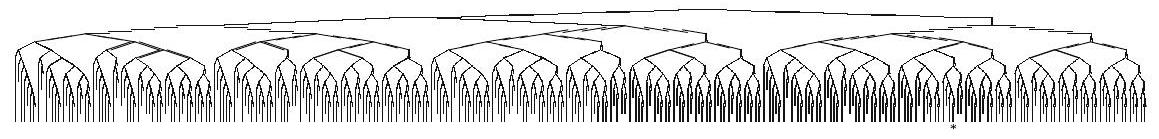
\includegraphics[max width=\textwidth, center]{2025_05_12_af19cd5e0d1b8a465ffeg-096}

The tree was cut off at a depth of 14 and has a solution in the leaf node marked by $*$. It is only possible to represent it at all because of the small branching factor of at most two and a cutoff at depth 14. For realistic problems, the branching factor and depth of the first solution may become significantly bigger.

Assume the branching factor is a constant equal to 30 and the first solution is at depth 50. The search tree has $30^{50} \approx 7.2 \times 10^{73}$ leaf nodes. But the number of inference steps is even bigger because not only every leaf node, but also every inner node of the tree corresponds to an inference step. Therefore we must add up the nodes over all levels and obtain the total number of nodes of the search tree

$$
\sum_{d=0}^{50} 30^{d}=\frac{1-30^{51}}{1-30}=7.4 \times 10^{73}
$$

which does not change the node count by much. Evidently, nearly all of the nodes of this search tree are on the last level. As we will see, this is generally the case. But now back to the search tree with the $7.4 \times 10^{73}$ nodes. Assume we had 10,000\\
computers which can each perform a billion inferences per second, and that we could distribute the work over all of the computers with no cost. The total computation time for all $7.4 \times 10^{73}$ inferences would be approximately equal to

$$
\frac{7.4 \times 10^{73} \text { inferences }}{10000 \times 10^{9} \text { inferences } / \mathrm{sec}}=7.4 \times 10^{60} \mathrm{sec} \approx 2.3 \times 10^{53} \text { years }
$$

which is about $10^{43}$ times as much time as the age of our universe. By this simple thought exercise, we can quickly recognize that there is no realistic chance of searching this kind of search space completely with the means available to us in this world. Moreover, the assumptions related to the size of the search space were completely realistic. In chess for example, there are over 30 possible moves for a typical situation, and a game lasting 50 half-turns is relatively short.

How can it be then, that there are good chess players-and these days also good chess computers? How can it be that mathematicians find proofs for theorems in which the search space is even much bigger? Evidently we humans use intelligent strategies which dramatically reduce the search space. The experienced chess player, just like the experienced mathematician, will, by mere observation of the situation, immediately rule out many actions as senseless. Through his experience, he has the ability to evaluate various actions for their utility in reaching the goal. Often a person will go by feel. If one asks a mathematician how he found a proof, he may answer that the intuition came to him in a dream. In difficult cases, many doctors find a diagnosis purely by feel, based on all known symptoms. Especially in difficult situations, there is often no formal theory for solution-finding that guarantees an optimal solution. In everyday problems, such as the search for a runaway cat in Fig. 6.1 on page 93, intuition plays a big role. We will deal with this kind of heuristic search method in Sect. 6.3 and additionally describe processes with which computers can, similarly to humans, improve their heuristic search strategies by learning.

First, however, we must understand how uninformed search, that is, blindly trying out all possibilities, works. We begin with a few examples.

Example 6.1 With the 8-puzzle, a classic example for search algorithms [Nil98, RN10], the various algorithms can be very visibly illustrated. Squares with the numbers 1 to 8 are distributed in a $3 \times 3$ matrix like the one in Fig. 6.2 on page 93. The goal is to reach a certain ordering of the squares, for example in ascending order by rows as represented in Fig. 6.2 on page 93. In each step a square can be moved left, right, up, or down into the empty space. The empty space therefore moves in the corresponding opposite direction. For analysis of the search space, it is convenient to always look at the possible movements of the empty field.

The search tree for a starting state is represented in Fig. 6.3 on page 94. We can see that the branching factor alternates between two, three, and four. Averaged over two levels at a time, we obtain an average branching factor ${ }^{1}$ of $\sqrt{8} \approx 2.83$. We see

\footnotetext{${ }^{1}$ The average branching factor of a tree is the branching factor that a tree with a constant branching factor, equal depth, and an equal amount of leaf nodes would have.
}
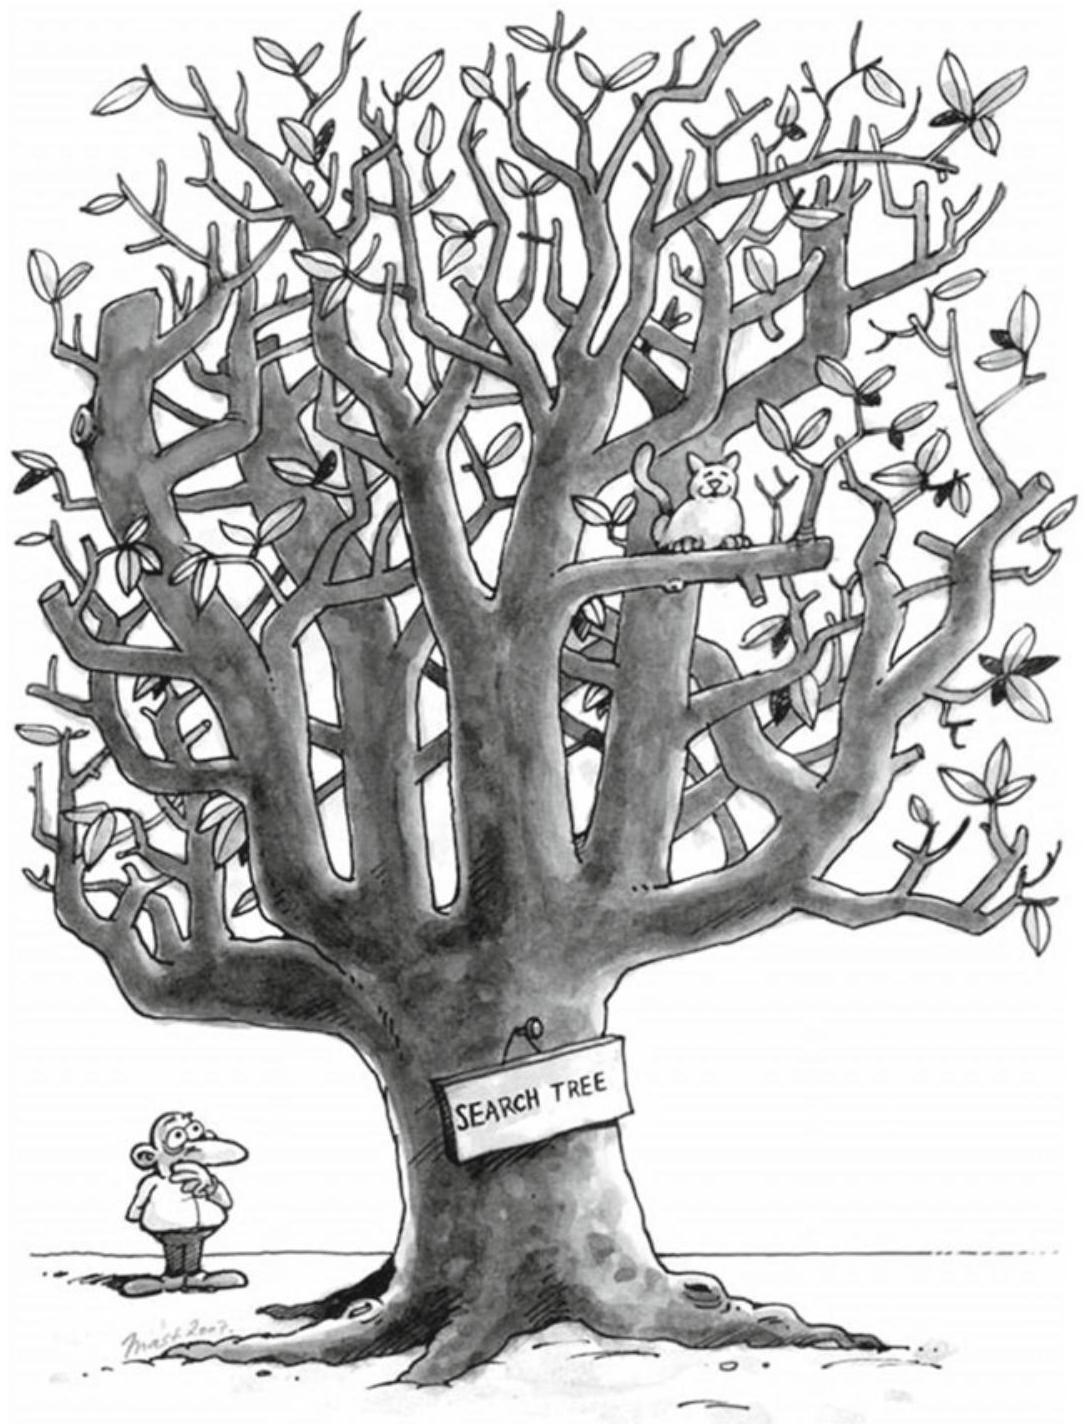
\includegraphics[max width=\textwidth, center]{2025_05_12_af19cd5e0d1b8a465ffeg-098(1)}

Fig. 6.1 A heavily trimmed search tree-or: "Where is my cat?"

Fig. 6.2 Possible starting and goal states of the 8-puzzle\\
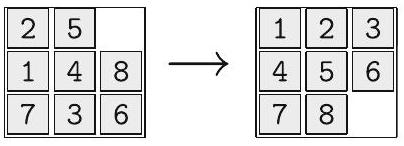
\includegraphics[max width=\textwidth, center]{2025_05_12_af19cd5e0d1b8a465ffeg-098}\\
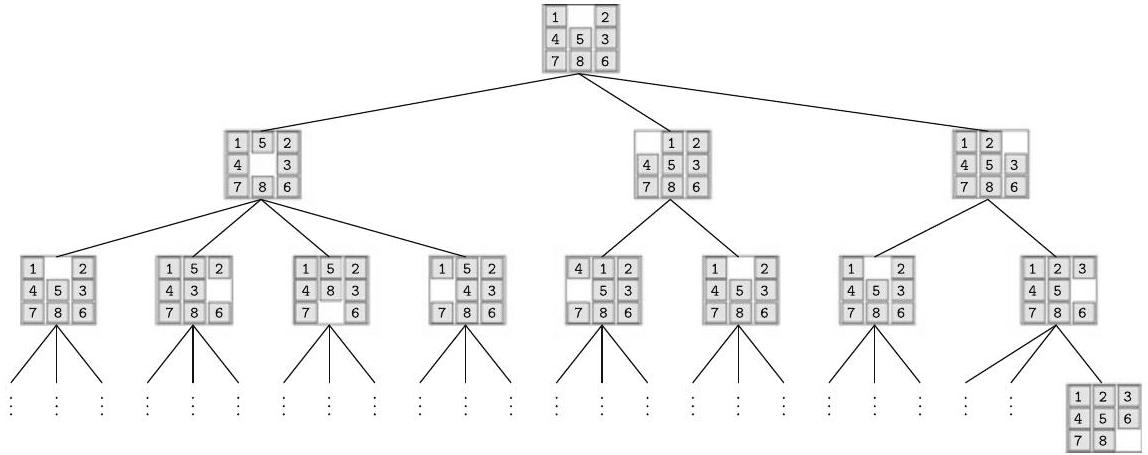
\includegraphics[max width=\textwidth, center]{2025_05_12_af19cd5e0d1b8a465ffeg-099}

Fig. 6.3 Search tree for the 8 -puzzle. Bottom right a goal state in depth 3 is represented. To save space the other nodes at this level have been omitted\\
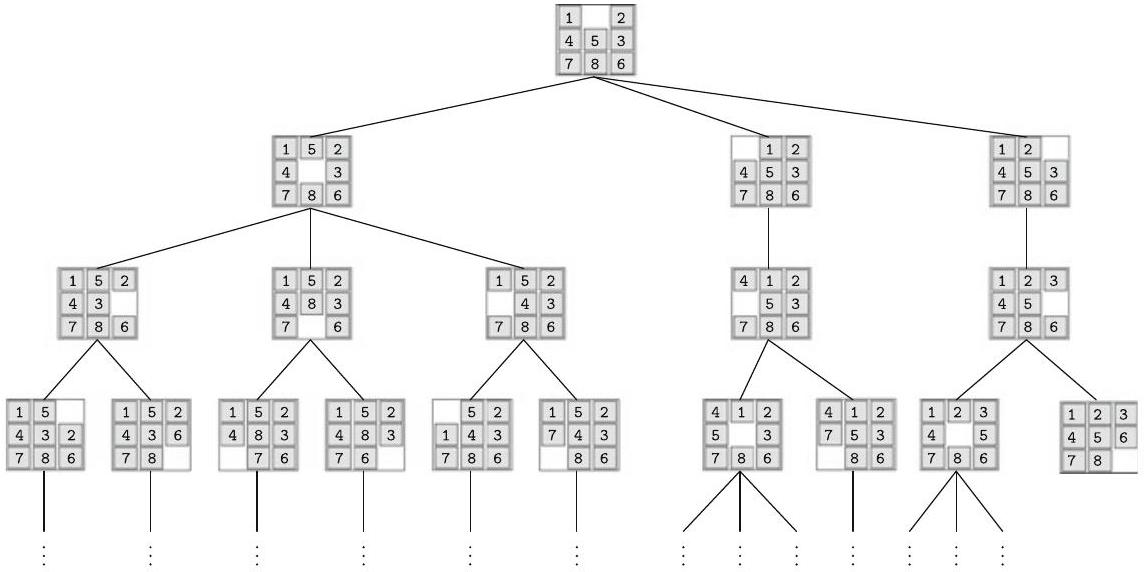
\includegraphics[max width=\textwidth, center]{2025_05_12_af19cd5e0d1b8a465ffeg-099(1)}

Fig. 6.4 Search tree for an 8-puzzle without cycles of length 2\\
that each state is repeated multiple times two levels deeper because in a simple uninformed search, every action can be reversed in the next step.

If we disallow cycles of length 2 , then for the same starting state we obtain the search tree represented in Fig. 6.4. The average branching factor is reduced by about 1 and becomes 1.8. ${ }^{2}$

Before we begin describing the search algorithms, a few new terms are needed. We are dealing with discrete search problems here. Being in state $s$, an action $a_{1}$ leads to a new state $s^{\prime}$. Thus $s^{\prime}=a_{1}(s)$. A different action may lead to state $s^{\prime \prime}$, in

\footnotetext{${ }^{2}$ For an 8-puzzle the average branching factor depends on the starting state (see Exercise 6.2 on page 122).
}
other words: $s^{\prime \prime}=a_{2}(s)$. Recursive application of all possible actions to all states, beginning with the starting state, yields the search tree.

Definition 6.1 A search problem is defined by the following values\\
State: Description of the state of the world in which the search agent finds itself.\\
Starting state: The initial state in which the search agent is started.\\
Goal state: If the agent reaches a goal state, then it terminates and outputs a solution (if desired).\\
Actions: All of the agents allowed actions.\\
Solution: The path in the search tree from the starting state to the goal state.\\
Cost function: Assigns a cost value to every action. Necessary for finding a cost-optimal solution.\\
State space: Set of all states.

Applied to the 8-puzzle, we get\\
State: $3 \times 3$ matrix $S$ with the values $1,2,3,4,5,6,7,8$ (once each) and one empty square.\\
Starting state: An arbitrary state.\\
Goal state: An arbitrary state, e.g. the state given to the right in Fig. 6.2 on page 93.\\
Actions: Movement of the empty square $S_{i j}$ to the left (if $j \neq 1$ ), right (if $j \neq 3$ ), up (if $i \neq 1$ ), down (if $i \neq 3$ ).\\
Cost function: The constant function 1, since all actions have equal cost.\\
State space: The state space is degenerate in domains that are mutually unreachable (Exercise 6.4 on page 122). Thus there are unsolvable 8-puzzle problems.\\
For analysis of the search algorithms, the following terms are needed:

\section*{Definition 6.2}
\begin{itemize}
  \item The number of successor states of a state $s$ is called the branching factor $b(s)$, or $b$ if the branching factor is constant.
  \item The effective branching factor of a tree of depth $d$ with $n$ total nodes is defined as the branching factor that a tree with constant branching factor, equal depth, and equal $n$ would have (see Exercise 6.3 on page 122).
  \item A search algorithm is called complete if it finds a solution for every solvable problem. If a complete search algorithm terminates without finding a solution, then the problem is unsolvable.
\end{itemize}

For a given depth $d$ and node count $n$, the effective branching factor can be calculated by solving the equation


\begin{equation*}
n=\frac{b^{d+1}-1}{b-1} \tag{6.1}
\end{equation*}


for $b$ because a tree with constant branching factor and depth $d$ has a total of


\begin{equation*}
n=\sum_{i=0}^{d} b^{i}=\frac{b^{d+1}-1}{b-1} \tag{6.2}
\end{equation*}


nodes.\\
For the practical application of search algorithms for finite search trees, the last level is especially important because

Theorem 6.1 For heavily branching finite search trees with a large constant branching factor, almost all nodes are on the last level.

The simple proof of this theorem is recommended to the reader as an exercise (Exercise 6.1 on page 122).

Example 6.2 We are given a map, such as the one represented in Fig. 6.5, as a graph with cities as nodes and highway connections between the cities as weighted edges with distances. We are looking for an optimal route from city $A$ to city $B$. The description of the corresponding schema reads\\
State: A city as the current location of the traveler.\\
Starting state: An arbitrary city.\\
Goal state: An arbitrary city.\\
Actions: Travel from the current city to a neighboring city.\\
Cost function: The distance between the cities. Each action corresponds to an edge in the graph with the distance as the weight.\\
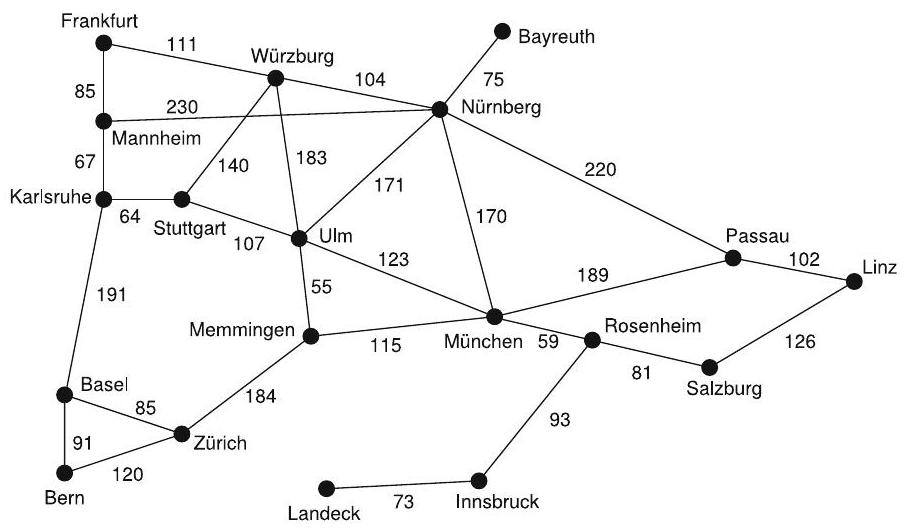
\includegraphics[max width=\textwidth, center]{2025_05_12_af19cd5e0d1b8a465ffeg-101}

Fig. 6.5 The graph of southern Germany as an example of a search task with a cost function

State space: All cities, that is, nodes of the graph.\\
To find the route with minimal length, the costs must be taken into account because they are not constant as they were in the 8-puzzle.

Definition 6.3 A search algorithm is called optimal if it, if a solution exists, always finds the solution with the lowest cost.

The 8-puzzle problem is deterministic, which means that every action leads from a state to a unique successor state. It is furthermore observable, that is, the agent always knows which state it is in. In route planning in real applications both characteristics are not always given. The action "Drive from Munich to Ulm" may-for example because of an accident-lead to the successor state "Munich". It can also occur that the traveler no longer knows where he is because he got lost. We want to ignore these kinds of complications at first. Therefore in this chapter we will only look at problems that are deterministic and observable.

Problems like the 8-puzzle, which are deterministic and observable, make action planning relatively simple because, due to having an abstract model, it is possible to find action sequences for the solution of the problem without actually carrying out the actions in the real world. In the case of the 8-puzzle, it is not necessary to actually move the squares in the real world to find the solution. We can find optimal solutions with so-called offline algorithms. One faces much different challenges when, for example, building robots that are supposed to play soccer. Here there will never be an exact abstract model of the actions. For example, a robot that kicks the ball in a specific direction cannot predict with certainty where the ball will move because, among other things, it does not know whether an opponent will catch or deflect the ball. Here online algorithms are then needed, which make decisions based on sensor signals in every situation. Reinforcement learning, described in Chap. 10, works toward optimization of these decisions based on experience.

\subsection*{6.2 Uninformed Search}
\subsection*{6.2.1 Breadth-First Search}
In breadth-first search, the search tree is explored from top to bottom according to the algorithm given in Fig. 6.6 on page 98 until a solution is found. First every node in the node list is tested for whether it is a goal node, and in the case of success, the program is stopped. Otherwise all successors of the node are generated. The search is then continued recursively on the list of all newly generated nodes. The whole thing repeats until no more successors are generated.

This algorithm is generic. That is, it works for arbitrary applications if the two application-specific functions "GoalReached" and "Successors" are provided.

\begin{verbatim}
BreadthFIrstSearch(NodeList, Goal)
NewNodes = Ø
For all Node \in NodeList
    If GoalReached(Node, Goal)
        Return("Solution found", Node)
    NewNodes = Append(NewNodes, Successors(Node))
If NewNodes # }\mp@code{ 0
    Return(BreADTH-FIRST-SEARCH(NewNodes, Goal))
Else
    Return("No solution")
\end{verbatim}

Fig. 6.6 The algorithm for breadth-first search\\
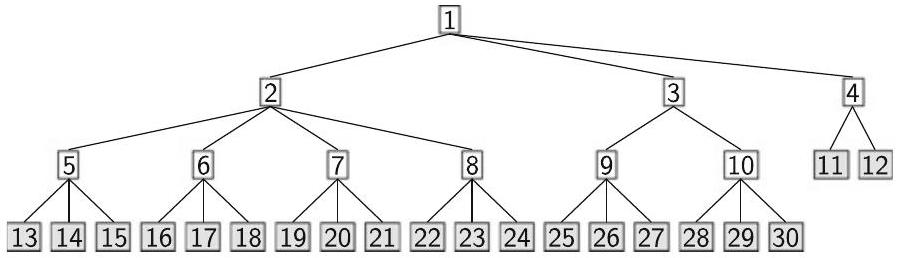
\includegraphics[max width=\textwidth, center]{2025_05_12_af19cd5e0d1b8a465ffeg-103}

Fig. 6.7 Breadth-first search during the expansion of the third-level nodes. The nodes are numbered according to the order they were generated. The successors of nodes 11 and 12 have not yet been generated\\
"GoalReached" calculates whether the argument is a goal node, and "Successors" calculates the list of all successor nodes of its argument. Figure 6.7 shows a snapshot of breadth-first search.

Analysis Since breadth-first search completely searches through every depth and reaches every depth in finite time, it is complete if the branching factor $b$ is finite. The optimal (that is, the shortest) solution is found if the costs of all actions are the same (see Exercise 6.7 on page 123). Computation time and memory space grow exponentially with the depth of the tree. For a tree with constant branching factor $b$ and depth $d$, the total compute time is thus given by

$$
c \cdot \sum_{i=0}^{d} b^{i}=\frac{b^{d+1}-1}{b-1}=O\left(b^{d}\right) .
$$

Although only the last level is saved in memory, the memory space requirement is also $O\left(b^{d}\right)$.

With the speed of today's computers, which can generate billions of nodes within minutes, main memory quickly fills up and the search ends. The problem of the shortest solution not always being found can be solved by the so-called Uniform Cost Search, in which the node with the lowest cost from the list of nodes (which is sorted ascendingly by cost) is always expanded, and the new nodes sorted in. Thus we find the optimal solution. The memory problem is not yet solved, however. A solution for this problem is provided by depth-first search.

\subsection*{6.2.2 Depth-First Search}
In depth-first search only a few nodes are stored in memory at one time. After the expansion of a node only its successors are saved, and the first successor node is immediately expanded. Thus the search quickly becomes very deep. Only when a node has no successors and the search fails at that depth is the next open node expanded via backtracking to the last branch, and so on. We can best perceive this in the elegant recursive algorithm in Fig. 6.8 and in the search tree in Fig. 6.9 on page 100.\\
Analysis Depth-first search requires much less memory than breadth-first search because at most $b$ nodes are saved at each depth. Thus we need at most $b \cdot d$ memory cells.

However, depth-first search is not complete for infinitely deep trees because depth-first search runs into an infinite loop when there is no solution in the far left branch. Therefore the question of finding the optimal solution is obsolete. Because of the infinite loop, no bound on the computation time can be given. In the case of a finitely deep search tree with depth $d$, a total of about $b^{d}$ nodes are generated. Thus the computation time grows, just as in breadth-first search, exponentially with depth.

We can make the search tree finite by setting a depth limit. Now if no solution is found in the pruned search tree, there can nonetheless be solutions outside the limit.

\begin{verbatim}
DEPTHFIRSTSEARCH(Node, Goal)
If GoalReached(Node, Goal) Return("Solution found")
NewNodes = Successors(Node)
While NewNodes # }=
    Result = DEPTH-FIRST-SEARCH(First(NewNodes), Goal)
    If Result = "Solution found" Return("Solution found")
    NewNodes = Rest(NewNodes)
Return("No solution")
\end{verbatim}

Fig. 6.8 The algorithm for depth-first search. The function "First" returns the first element of a list, and "Rest" the rest of the list\\
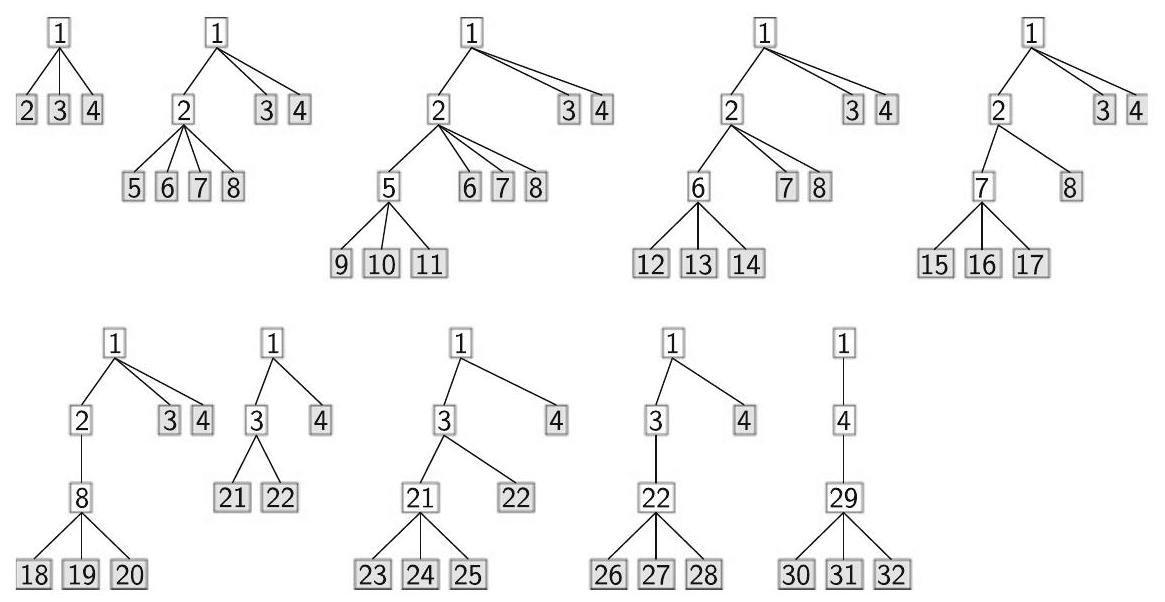
\includegraphics[max width=\textwidth, center]{2025_05_12_af19cd5e0d1b8a465ffeg-105(1)}

Fig. 6.9 Execution of depth-first search. All nodes at depth three are unsuccessful and cause backtracking. The nodes are numbered in the order they were generated\\
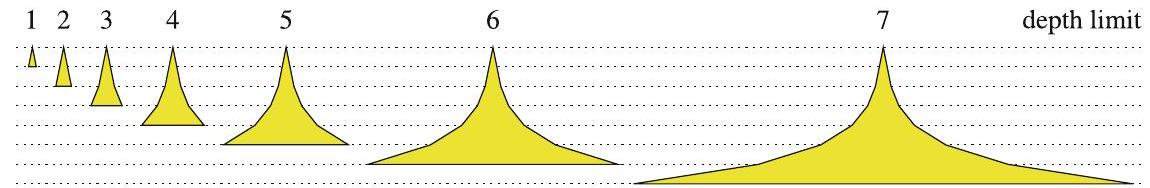
\includegraphics[max width=\textwidth, center]{2025_05_12_af19cd5e0d1b8a465ffeg-105}

Fig. 6.10 Schematic representation of the development of the search tree in iterative deepening with limits from 1 to 7 . The breadth of the tree corresponds to a branching factor of 2

Thus the search becomes incomplete. There are obvious ideas, however, for getting the search to completeness.

\subsection*{6.2.3 Iterative Deepening}
We begin the depth-first search with a depth limit of 1 . If no solution is found, we raise the limit by 1 and start searching from the beginning, and so on, as shown in Fig. 6.10. This iterative raising of the depth limit is called iterative deepening.

We must augment the depth-first search program given in Fig. 6.8 on page 99 with the two additional parameters "Depth" and "Limit". "Depth" is raised by one at the recursive call, and the head line of the while loop is replaced by "While NewNodes $\neq \emptyset$ And Depth < Limit". The modified algorithm is represented in Fig. 6.11 on page 101.

Analysis The memory requirement is the same as in depth-first search. One could argue that repeatedly re-starting depth-first search at depth zero causes a lot of redundant work. For large branching factors this is not the case. We now show that\\
IterativeDeepening(Node, Goal)\\
DepthLimit $=0$\\
Repeat\\
Result = DepthFirstSearch-B(Node, Goal, 0, DepthLimit)\\
DepthLimit = DepthLimit + 1\\
Until Result = "Solution found"\\
DepthFirstSearch-B(Node, Goal, Depth, Limit)\\
If GoalReached(Node, Goal) Return("Solution found")\\
NewNodes = Successors(Node)\\
While NewNodes $\neq \emptyset$ And Depth $<$ Limit\\
Result =\\
DepthFirstSearch-B(First(NewNodes), Goal, Depth +1 , Limit)\\
If Result = "Solution found" Return("Solution found")\\
NewNodes = Rest(NewNodes)\\
Return("No solution")

Fig. 6.11 The algorithm for iterative deepening, which calls the slightly modified depth-first search with a depth limit (Tiefensuche-B)\\
the sum of the number of nodes of all depths up to the one before last $d_{\text {max }}-1$ in all trees searched is much smaller than the number of nodes in the last tree searched.

Let $N_{b}(d)$ be the number of nodes of a search tree with branching factor $b$ and depth $d$ and $d_{\text {max }}$ be the last depth searched. The last tree searched contains

$$
N_{b}\left(d_{\max }\right)=\sum_{i=0}^{d_{\max }} b^{i}=\frac{b^{d_{\max }+1}-1}{b-1}
$$

nodes. All trees searched beforehand together have

$$
\begin{aligned}
\sum_{d=1}^{d_{\max }-1} N_{b}(d) & =\sum_{d=1}^{d_{\max }-1} \frac{b^{d+1}-1}{b-1}=\frac{1}{b-1}\left(\left(\sum_{d=1}^{d_{\max }-1} b^{d+1}\right)-d_{\max }+1\right) \\
& =\frac{1}{b-1}\left(\left(\sum_{d=2}^{d_{\max }} b^{d}\right)-d_{\max }+1\right) \\
& =\frac{1}{b-1}\left(\frac{b^{d_{\max }+1}-1}{b-1}-1-b-d_{\max }+1\right) \\
& \approx \frac{1}{b-1}\left(\frac{b^{d_{\max }+1}-1}{b-1}\right)=\frac{1}{b-1} N_{b}\left(d_{\max }\right)
\end{aligned}
$$

nodes. For $b>2$ this is less than the number $N_{b}\left(d_{\max }\right)$ of nodes in the last tree. For $b=20$ the first $d_{\text {max }}-1$ trees together contain only about $\frac{1}{b-1}=1 / 19$ of the number of nodes in the last tree. The computation time for all iterations besides the last can be ignored.

Just like breadth-first search, this method is complete, and given a constant cost for all actions, it finds the shortest solution.

\subsection*{6.2.4 Comparison}
The described search algorithms have been put side-by-side in Table 6.1.\\
We can clearly see that iterative deepening is the winner of this test because it gets the best grade in all categories. In fact, of all four algorithms presented it is the only practically usable one.

We do indeed have a winner for this test, although for realistic applications it is usually not successful. Even for the 15 -puzzle, the 8 -puzzle's big brother (see Exercise 6.4 on page 122), there are about $2 \times 10^{13}$ different states. For non-trivial inference systems the state space is many orders of magnitude bigger. As shown in Sect. 6.1, all the computing power in the world will not help much more. Instead what is needed is an intelligent search that only explores a tiny fraction of the search space and finds a solution there.

\subsection*{6.2.5 Cycle Check}
As shown in Sect. 6.1, nodes may be repeatedly visited during a search. In the 8-puzzle, for example, every move can be immediately undone, which leads to unnecessary cycles of length two. Such cycles can be prevented by recording within each node all of its predecessors and, when expanding a node, comparing the newly created successor nodes with the predecessor nodes. All of the duplicates found can be removed from the list of successor nodes. This simple check costs only a small constant factor of additional memory space and increases the constant computation time $c$ by an additional constant $\delta$ for the check itself for a total of $c+\delta$. This overhead for the cycle check is (hopefully) offset by a reduction in the cost of the

Table 6.1 Comparison of the uninformed search algorithms. (*) means that the statement is only true given a constant action cost. $d_{s}$ is the maximal depth for a finite search tree

\begin{center}
\begin{tabular}{|l|l|l|l|l|}
\hline
 & Breadth-first search & Uniform cost search & Depth-first search & Iterative deepening \\
\hline
Completeness & Yes & Yes & No & Yes \\
\hline
Optimal solution & Yes (*) & Yes & No & Yes (*) \\
\hline
Computation time & $b^{d}$ & $b^{d}$ & $\infty$ or $b^{d}$ & $b^{d}$ \\
\hline
Memory use & $b^{d}$ & $b^{d}$ & $b d$ & bd \\
\hline
\end{tabular}
\end{center}

search. The reduction depends, of course, on the particular application and therefore cannot be given in general terms.

For the 8 -puzzle we obtain the result as follows. If, for example, during breadth-first search with effective branching factor $b$ on a finite tree of depth $d$, the computation time without the cycle check is $c \cdot b^{d}$, the required time with the cycle check becomes

$$
(c+\delta) \cdot(b-1)^{d}
$$

The check thus practically always results in a clear gain because reducing the branching factor by one has an exponentially growing effect as the depth increases, whereas the additional computation time $\delta$ only somewhat increases the constant factor.

Now the question arises as to how a check on cycles of arbitrary length would affect the search performance. The list of all predecessors must now be stored for each node, which can be done very efficiently (see Exercise 6.8 on page 123). During the search, each newly created node must now be compared with all its predecessors. The computation time of depth-first search or breadth-first search is given by

$$
c_{1} \cdot \sum_{i=0}^{d} b^{i}+c_{2} \cdot \sum_{i=0}^{d} i \cdot b^{i}
$$

Here, the first term is the already-known cost of generating the nodes, and the second term is the cost of the cycle check. We can show that for large values of $b$ and $d$,

$$
\sum_{i=0}^{d} i \cdot b^{i} \approx d \cdot b^{d} .
$$

The complexity of the search with the full cycle check therefore only increases by a factor of $d$ faster than for the search without a cycle check. In search trees that are not very deep, this extra complexity is not important. For search tasks with very deep, weakly branching trees, it may be advantageous to use a hash table [CLR90] to store the list of predecessors. Lookups in the table can be done in constant time such that the computation time of the search algorithm only grows by a small constant factor.

In summary, we can conclude that the cycle check implies hardly any additional overhead and is therefore worthwhile for applications with repeatedly occurring nodes.

\subsection*{6.3 Heuristic Search}
Heuristics are problem-solving strategies which in many cases find a solution faster than uninformed search. However, this is not guaranteed. Heuristic search could require a lot more time and can even result in the solution not being found.

We humans successfully use heuristic processes for all kinds of things. When buying vegetables at the supermarket, for example, we judge the various options for a pound of strawberries using only a few simple criteria like price, appearance, source of production, and trust in the seller, and then we decide on the best option by gut feeling. It might theoretically be better to subject the strawberries to a basic chemical analysis before deciding whether to buy them. For example, the strawberries might be poisoned. If that were the case the analysis would have been worth the trouble. However, we do not carry out this kind of analysis because there is a very high probability that our heuristic selection will succeed and will quickly get us to our goal of eating tasty strawberries.

Heuristic decisions are closely linked with the need to make real-time decisions with limited resources. In practice a good solution found quickly is preferred over a solution that is optimal, but very expensive to derive.

A heuristic evaluation function $f(s)$ for states is used to mathematically model a heuristic. The goal is to find, with little effort, a solution to the stated search problem with minimal total cost. Please note that there is a subtle difference between the effort to find a solution and the total cost of this solution. For example it may take Google Maps half a second's worth of effort to find a route from the City Hall in San Francisco to Tuolumne Meadows in Yosemite National Park, but the ride from San Francisco to Tuolumne Meadows by car may take four hours and some money for gasoline etc. (total cost).

Next we will modify the breadth-first search algorithm by adding the evaluation function to it. The currently open nodes are no longer expanded left to right by row, but rather according to their heuristic rating. From the set of open nodes, the node with the minimal rating is always expanded first. This is achieved by immediately evaluating nodes as they are expanded and sorting them into the list of open nodes. The list may then contain nodes from different depths in the tree.

Because heuristic evaluation of states is very important for the search, we will differentiate from now on between states and their associated nodes. The node contains the state and further information relevant to the search, such as its depth in the search tree and the heuristic rating of the state. As a result, the function "Successors", which generates the successors (children) of a node, must also immediately calculate for these successor nodes their heuristic ratings as a component of each node. We define the general search algorithm HeuristicSearch in Fig. 6.12 on page 105.

The node list is initialized with the starting nodes. Then, in the loop, the first node from the list is removed and tested for whether it is a solution node. If not, it will be expanded with the function "Successors" and its successors added to the list with the function "SortIn". "SortIn(X,Y)" inserts the elements from the unsorted list X into the ascendingly sorted list Y. The heuristic rating is used as the sorting key. Thus it is guaranteed that the best node (that is, the one with the lowest heuristic value) is always at the beginning of the list. ${ }^{3}$

\footnotetext{${ }^{3}$ When sorting in a new node from the node list, it may be advantageous to check whether the node is already available and, if so, to delete the duplicate.
}\begin{verbatim}
HeuristicSearch(Start, Goal)
NodeList = [Start]
While True
    If NodeList = Ø Return("No solution")
    Node = First(NodeList)
    NodeList = Rest(NodeList)
    If GoalReached(Node, Goal) Return("Solution found", Node)
    NodeList = SortIn(Successors(Node),NodeList)
\end{verbatim}

Fig. 6.12 The algorithm for heuristic search\\
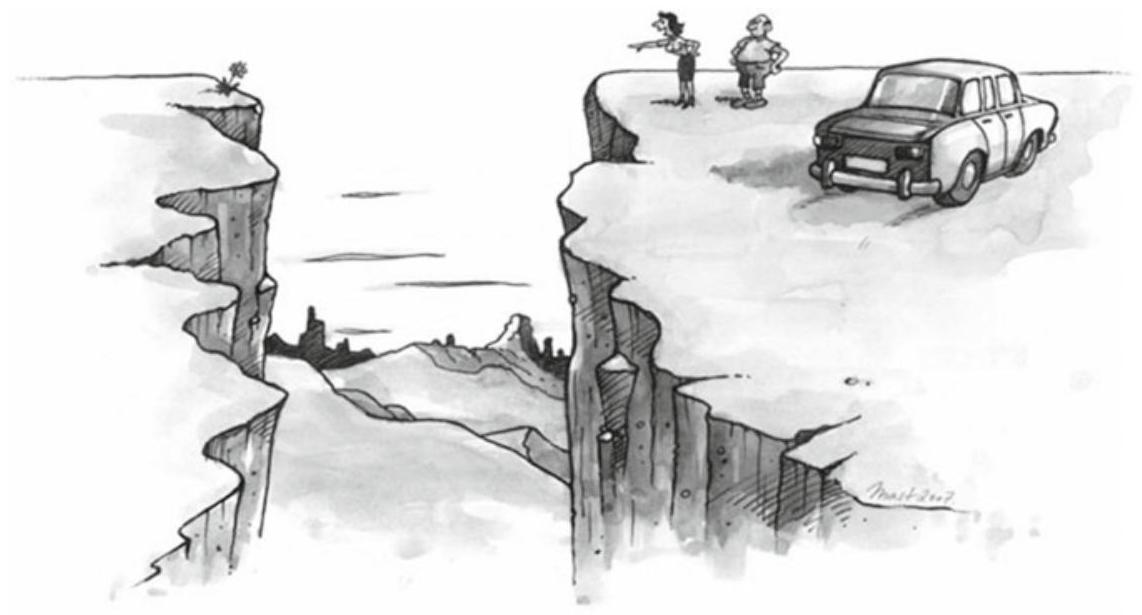
\includegraphics[max width=\textwidth, center]{2025_05_12_af19cd5e0d1b8a465ffeg-110}

Fig. 6.13 He: "Dear, think of the fuel cost! I'll pluck one for you somewhere else." She: "No, I want that one over there!"

Depth-first and breadth-first search also happen to be special cases of the function HeuristicSearch. We can easily generate them by plugging in the appropriate evaluation function (Exercise 6.11 on page 123).

The best heuristic would be a function that calculates the actual costs from each node to the goal. To do that, however, would require a traversal of the entire search space, which is exactly what the heuristic is supposed to prevent. Therefore we need a heuristic that is fast and simple to compute. How do we find such a heuristic?

An interesting idea for finding a heuristic is simplification of the problem. The original task is simplified enough that it can be solved with little computational cost. The costs from a state to the goal in the simplified problem then serve as an estimate for the actual problem (see Fig. 6.13). This cost estimate function we denote $h$.

\subsection*{6.3.1 Greedy Search}
It seems sensible to choose the state with the lowest estimated $h$ value (that is, the one with the lowest estimated cost) from the list of currently available states. The cost estimate then can be used directly as the evaluation function. For the evaluation in the function HeuristicSearch we set $f(s)=h(s)$. This can be seen clearly in the trip planning example (Example 6.2 on page 96). We set up the task of finding the straight line path from city to city (that is, the flying distance) as a simplification of the problem. Instead of searching the optimal route, we first determine from every node a route with minimal flying distance to the goal. We choose Ulm as the destination. Thus the cost estimate function becomes

$$
h(s)=\text { flying distance from city } s \text { to Ulm. }
$$

The flying distances from all cities to Ulm are given in Fig. 6.14 next to the graph.\\
The search tree for starting in Linz is represented in Fig. 6.15 on page 107 left. We can see that the tree is very slender. The search thus finishes quickly. Unfortunately, this search does not always find the optimal solution. For example, this algorithm fails to find the optimal solution when starting in Mannheim (Fig. 6.15 on page 107 right). The Mannheim-Nürnberg-Ulm path has a length of 401 km . The route Mannheim-Karlsruhe-Stuttgart-Ulm would be significantly shorter at 238 km . As we observe the graph, the cause of this problem becomes clear. Nürnberg is in fact somewhat closer than Karlsruhe to Ulm, but the distance from Mannheim to Nürnberg is significantly greater than that from Mannheim to Karlsruhe. The heuristic only looks ahead "greedily" to the goal instead of also taking into account the stretch that has already been laid down to the current node. This is why we give it the name greedy search.\\
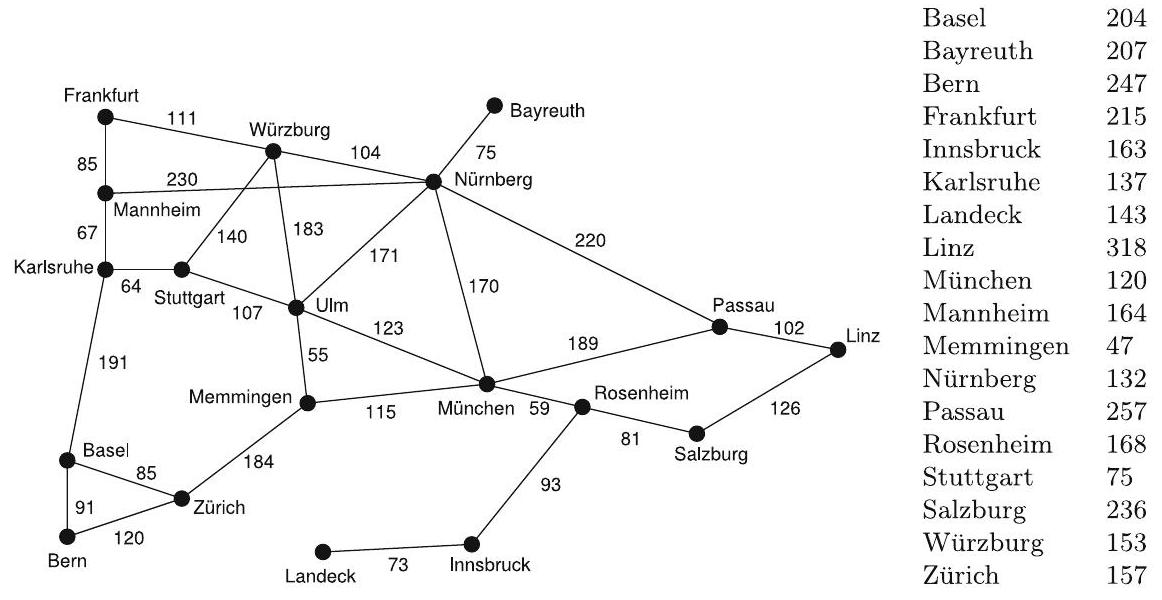
\includegraphics[max width=\textwidth, center]{2025_05_12_af19cd5e0d1b8a465ffeg-111}

Fig. 6.14 City graph with flying distances from all cities to Ulm\\
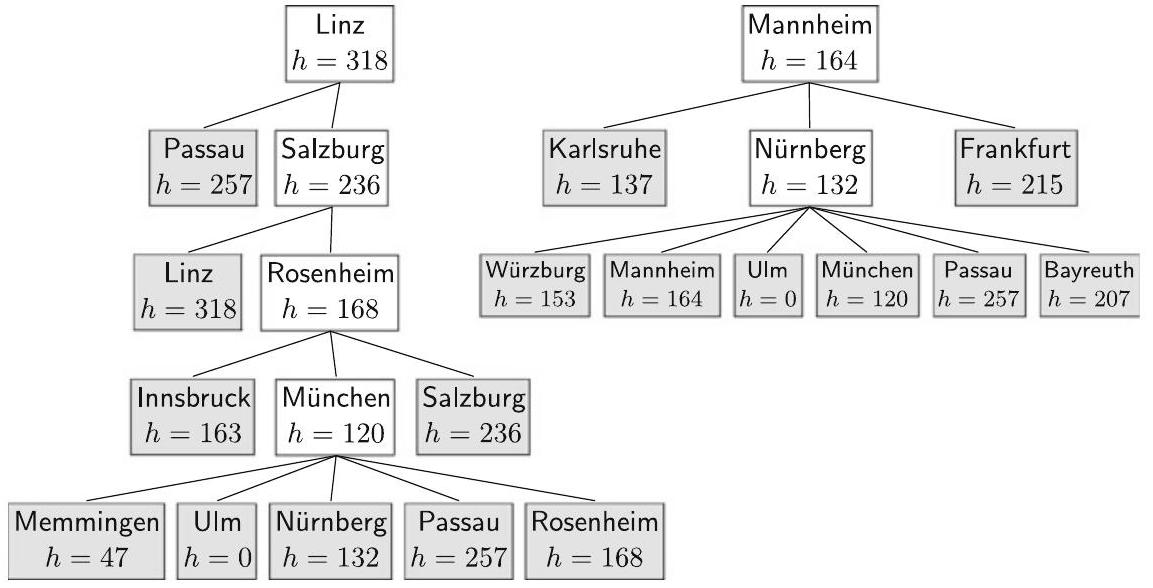
\includegraphics[max width=\textwidth, center]{2025_05_12_af19cd5e0d1b8a465ffeg-112}

\begin{center}
\begin{tabular}{|l||c|c|c|c|c|}
\hline
Node & München & Innsbruck & Salzburg & Passau & Linz \\
\hline
heuristic rating & 120 & 163 & 236 & 257 & 318 \\
\hline
\end{tabular}
\end{center}

Fig. 6.15 Greedy search: from Linz to Ulm (left) and from Mannheim to Ulm (right). The node list data structure for the left search tree, sorted by the node rating before the expansion of the node München is given

\subsection*{6.3.2 A ${ }^{\star}$-Search}
We now want to take into account the costs that have accrued during the search up to the current node $s$. First we define the cost function

$$
g(s)=\text { Sum of accrued costs from the start to the current node, }
$$

then add to that the estimated cost to the goal and obtain as the heuristic evaluation function

$$
f(s)=g(s)+h(s)
$$

Now we add yet another small, but important requirement.

Definition 6.4 A heuristic cost estimate function $h(s)$ that never overestimates the actual cost from state $s$ to the goal is called admissible.

The function HeuristicSearch together with an evaluation function $f(s)=g(s)+h(s)$ and an admissible heuristic function $h$ is called $\mathrm{A}^{\star}$-algorithm. This famous algorithm is complete and optimal. $A^{\star}$ thus always finds the shortest solution for every solvable search problem. We will explain and prove this in the following discussion.\\
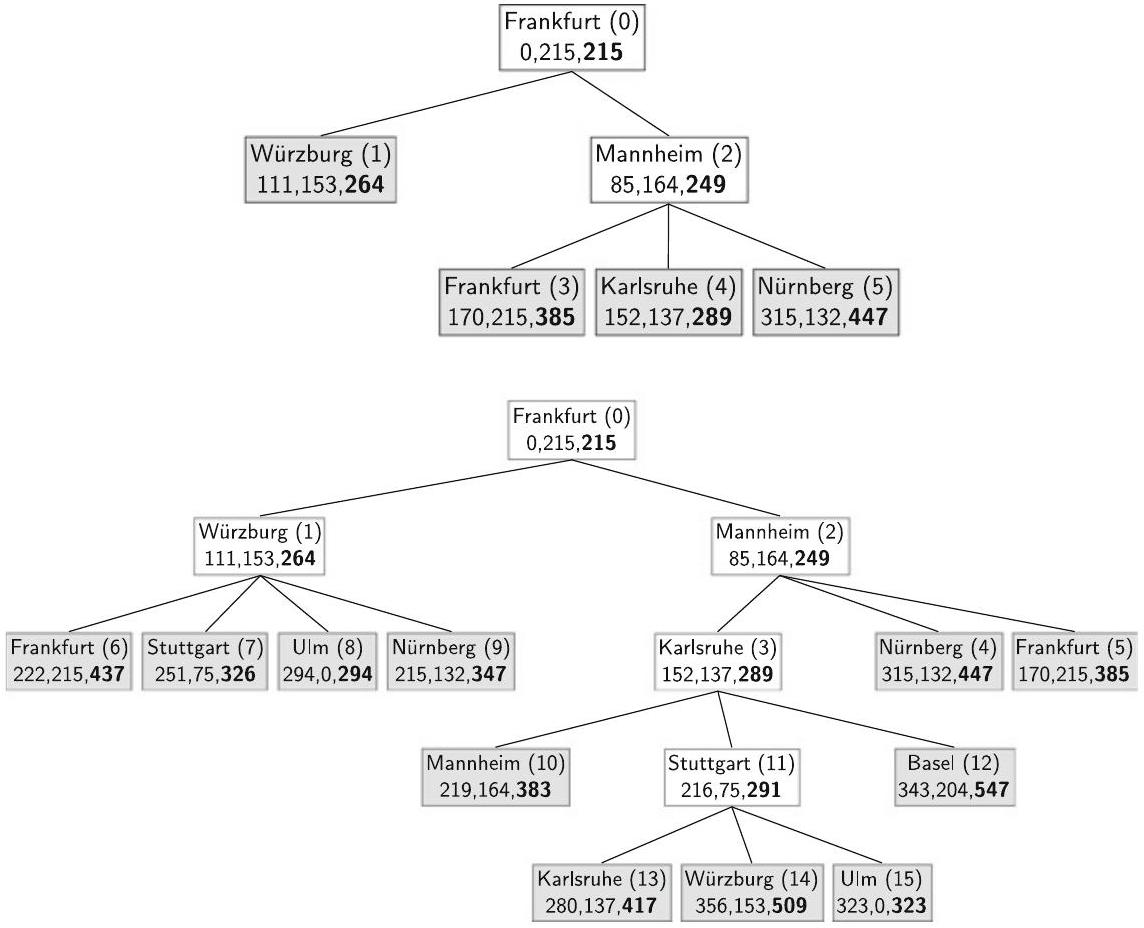
\includegraphics[max width=\textwidth, center]{2025_05_12_af19cd5e0d1b8a465ffeg-113}

Fig. 6.16 Two snapshots of the $A^{\star}$ search tree for the optimal route from Frankfurt to Ulm. In the boxes below the name of the city $s$ we show $g(s), h(s), f(s)$. Numbers in parentheses after the city names show the order in which the nodes have been generated by the "Successor" function

First we apply the $A^{\star}$-algorithm to the example. We are looking for the shortest path from Frankfurt to Ulm.

In the top part of Fig. 6.16 we see that the successors of Mannheim are generated before the successors of Würzburg. The optimal solution Frankfurt-Würzburg-Ulm is generated shortly thereafter in the eighth step, but it is not yet recognized as such. Thus the algorithm does not terminate yet because the node Karlsruhe (3) has a better (lower) $f$ value and thus is ahead of the node Ulm (8) in line. Only when all $f$ values are greater than or equal to that of the solution node Ulm (8) have we ensured that we have an optimal solution. Otherwise there could potentially be another solution with lower costs. We will now show that this is true generally.

Theorem 6.2 The $A^{\star}$ algorithm is optimal. That is, it always finds the solution with the lowest total cost if the heuristic $h$ is admissible.

Proof In the HeuristicSearch algorithm, every newly generated node $s$ is sorted in by the function "SortIn" according to its heuristic rating $f(s)$. The node with the

Fig. 6.17 The first solution node $l$ found by $\mathrm{A}^{\star}$ never has a higher cost than another arbitrary node $l^{\prime}$\\
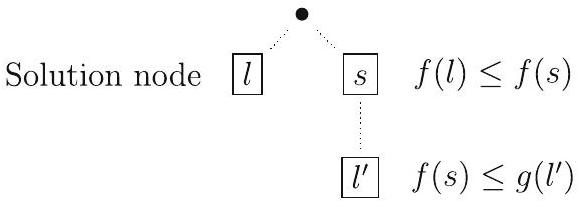
\includegraphics[max width=\textwidth, center]{2025_05_12_af19cd5e0d1b8a465ffeg-114}\\
smallest rating value thus is at the beginning of the list. If the node $l$ at the beginning of the list is a solution node, then no other node has a better heuristic rating. For all other nodes $s$ it is true then that $f(l) \leq f(s)$. Because the heuristic is admissible, no better solution $l^{\prime}$ can be found, even after expansion of all other nodes (see Fig. 6.17). Written formally:

$$
g(l)=g(l)+h(l)=f(l) \leq f(s)=g(s)+h(s) \leq g\left(l^{\prime}\right)
$$

The first equality holds because $l$ is a solution node with $h(l)=0$. The second is the definition of $f$. The third (in)equality holds because the list of open nodes is sorted in ascending order. The fourth equality is again the definition of $f$. Finally, the last (in)equality is the admissibility of the heuristic, which never overestimates the cost from node $s$ to an arbitrary solution. Thus it has been shown that $g(l) \leq g\left(l^{\prime}\right)$, that is, that the discovered solution $l$ is optimal.

\subsection*{6.3.3 Route Planning with the $\mathbf{A}^{\star}$ Search Algorithm}
Many current car navigation systems use the $A^{\star}$ algorithm. The simplest, but very good heuristic for computing $\mathrm{A}^{\star}$ is the straight-line distance from the current node to the destination. The use of 5 to 60 so-called landmarks is somewhat better. For these randomly chosen points the shortest paths to and from all nodes on the map are calculated in a precomputation step. Let $l$ be such a landmark, $s$ the current node, and $z$ the destination node. Also let $c^{\star}(x, y)$ be the cost of the shortest path from $x$ to $y$. Then we obtain for the shortest path from $s$ to $l$ the triangle inequality (see Exercise 6.11 on page 123)

$$
c^{\star}(s, l) \leq c^{\star}(s, z)+c^{\star}(z, l) .
$$

Solving for $c^{\star}(s, z)$ results in the admissible heuristic

$$
h(s)=c^{\star}(s, l)-c^{\star}(z, l) \leq c^{\star}(s, z) .
$$

In [Bat16], it was shown that this heuristic is better than the straight-line distance for route planning. On one hand, it can be calculated faster than the straight-line distance. Due to precomputation, distances to the landmarks can be quickly retrieved\\
from an array, whereas the Euclidean distances must be computed individually. It turns out that the landmark heuristic shrinks the search space even more. This can be seen in the left image of Fig. 6.18, which illustrates the search tree of $A^{\star}$ search for planning a route from Ravensburg to Biberach (two towns in southern Germany). ${ }^{4}$ The edges without any heuristic (i.e. with $h(s)=0$ ) are plotted in red colour, dark green lines show the search tree using the straight-line distance heuristic, and the edges of the landmark heuristic with twenty landmarks are plotted in blue.

The right image shows the same route using bidirectional search, where a route from Ravensburg to Biberach and one in the opposite direction are planned effectively in parallel. If the routes meet, given certain conditions of the heuristic, an optimal route has been found [Bat16]. A quantitative analysis of the search tree sizes and the computation time on a PC can be found in Table 6.2.\\
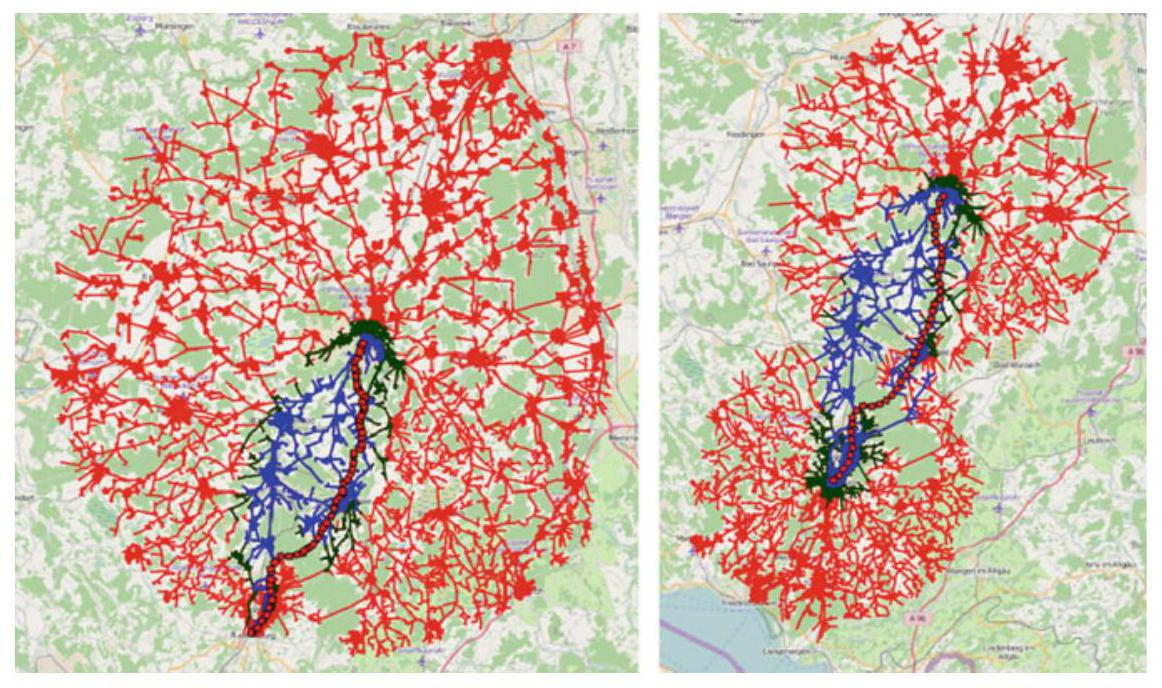
\includegraphics[max width=\textwidth, center]{2025_05_12_af19cd5e0d1b8a465ffeg-115}

Fig. $6.18 \mathrm{~A}^{\star}$ search tree without heuristic (red), with straight-line distance (dark green) and with landmarks (blue). The left image shows unidirectional search and the right shows bidirectional search. Note that the green edges are covered by blue and the red edges are covered by green and blue

Table 6.2 Comparison of search tree size and computation time for route planning with and without each of the two heuristics. The landmark heuristic is the clear winner

\begin{center}
\begin{tabular}{|l|l|l|l|l|}
\hline
\multirow{2}{*}{} & \multicolumn{2}{|c|}{Unidirectional} & \multicolumn{2}{|c|}{Bidirectional} \\
\hline
 & Tree Size [nodes] & Comp. time [msec.] & Tree Size [nodes] & Comp. time [msec.] \\
\hline
No heuristic & 62000 & 192 & 41850 & 122 \\
\hline
Straight-line distance & 9380 & 86 & 12193 & 84 \\
\hline
Landmark heuristic & 5260 & 16 & 7290 & 16 \\
\hline
\end{tabular}
\end{center}

\footnotetext{${ }^{4}$ Both graphs in Fig. 6.18 were generated by A. Batzill using the system described in [Bat16].
}Observing unidirectional search, we see that both heuristics clearly reduce the search space. The computation times are truly interesting. In the case of the landmark heuristic, we see the computation time and the size of the search space reduced by a factor of about 12. The cost of computing the heuristic is thus insignificant. The straight-line distance, however, results in a search space reduction of a factor of 6.6, but only an improvement of a factor of 2.2 in run time due to the overhead of computing the euclidean distance.

In the case of bidirectional search, in contrast to unidirectional search, we see a significant reduction of the search space even without heuristic. On the other hand, the search space is larger than the unidirectional case for both heuristics. However, because the nodes are partitioned into two sorted lists in bidirectional search (see HeuristicSearch function in Fig. 6.12 on page 105), the lists are handled faster and the resulting computation times are roughly the same [Bat16].

When planning a route, usually the driver cares more about driving time than the distance driven. We should thus adjust the heuristic accordingly and replace straight-line distance $d(s, z)$ with time $t(s, z)=d(s, z) / v_{\text {max }}$. Here we have to divide by the maximum average velocity, which degrades the heuristic because it causes the heuristically estimated times to be much too small. The landmark heuristic, in contrast, builds on precomputed optimal routes and therefore does not degrade. Thus, as shown in [Bat16], the search for a time-optimized route using landmark heuristic is significantly faster than with the modified straight-line distance.

The contraction hierarchies algorithm performs even better than $A^{\star}$ with landmark heuristic. It is based on the idea of combining, in a precompution step, several edges into so-called shortcuts, which are then used to reduce the search space [GSSD08, Bat16].

\subsection*{6.3.4 IDA ${ }^{\star}$-Search}
The $A^{\star}$ search inherits a quirk from breadth-first search. It has to save many nodes in memory, which can lead to very high memory use. Furthermore, the list of open nodes must be sorted. Thus insertion of nodes into the list and removal of nodes from the list can no longer run in constant time, which increases the algorithm's complexity slightly. Based on the heapsort algorithm, we can structure the node list as a heap with logarithmic time complexity for insertion and removal of nodes (see [CLR90]).

Both problems can be solved-similarly to breadth-first search-by iterative deepening. We work with depth-first search and successively raise the limit. However, rather than working with a depth limit, here we use a limit for the heuristic evaluation $f(s)$. This process is called the IDA ${ }^{\star}$-algorithm.

\subsection*{6.3.5 Empirical Comparison of the Search Algorithms}
In $A^{\star}$, or (alternatively) IDA ${ }^{\star}$, we have a search algorithm with many good properties. It is complete and optimal. It can thus be used without risk. The most\\
important thing, however, is that it works with heuristics, and therefore can significantly reduce the computation time needed to find a solution. We would like to explore this empirically in the 8 -puzzle example.

For the 8 -puzzle there are two simple admissible heuristics. The heuristic $h_{1}$ simply counts the number of squares that are not in the right place. Clearly this heuristic is admissible. Heuristic $h_{2}$ measures the Manhattan distance. For every square the horizontal and vertical distances to that square's location in the goal state are added together. This value is then summed over all squares. For example, the Manhattan distance of the two states

\begin{center}
\begin{tabular}{|c|c|c|}
\hline
2 & 5 &  \\
\hline
1 & 4 & 8 \\
\hline
7 & 3 & 6 \\
\hline\hline
\end{tabular}
\end{center}$\quad$ and $\quad$\begin{tabular}{|c|c|c|}
\hline
1 & 2 & 3 \\
\hline
4 & 5 & 6 \\
\hline
7 & 8 &  \\
\hline
\end{tabular}

is calculated as

$$
h_{2}(s)=1+1+1+1+2+0+3+1=10 .
$$

The admissibility of the Manhattan distance is also obvious (see Exercise 6.13 on page 123).

The described algorithms were implemented in Mathematica. For a comparison with uninformed search, the $\mathrm{A}^{\star}$ algorithm with the two heuristics $h_{1}$ and $h_{2}$ and iterative deepening was applied to 132 randomly generated 8 -puzzle problems. The average values for the number of steps and computation time are given in Table 6.3. We see that the heuristics significantly reduce the search cost compared to uninformed search.

If we compare iterative deepening to $\mathrm{A}^{\star}$ with $h_{1}$ at depth 12 , for example, it becomes evident that $h_{1}$ reduces the number of steps by a factor of about 3,000 , but

Table 6.3 Comparison of the computation cost of uninformed search and heuristic search for solvable 8-puzzle problems with various depths. Measurements are in steps and seconds. All values are averages over multiple runs (see last column)

\begin{center}
\begin{tabular}{|l|l|l|l|l|l|l|l|}
\hline
\multirow[t]{3}{*}{Depth} & \multicolumn{2}{|c|}{Iterative deepening} & \multicolumn{4}{|c|}{A* algorithm} & \multirow[t]{3}{*}{Num. runs} \\
\hline
 & \multirow[t]{2}{*}{Steps} & \multirow{2}{*}{Time [sec]} & \multicolumn{2}{|c|}{Heuristic $h_{1}$} & \multicolumn{2}{|c|}{Heuristic $h_{2}$} &  \\
\hline
 &  &  & Steps & Time [sec] & Steps & Time [sec] &  \\
\hline
2 & 20 & 0.003 & 3.0 & 0.0010 & 3.0 & 0.0010 & 10 \\
\hline
4 & 81 & 0.013 & 5.2 & 0.0015 & 5.0 & 0.0022 & 24 \\
\hline
6 & 806 & 0.13 & 10.2 & 0.0034 & 8.3 & 0.0039 & 19 \\
\hline
8 & 6455 & 1.0 & 17.3 & 0.0060 & 12.2 & 0.0063 & 14 \\
\hline
10 & 50512 & 7.9 & 48.1 & 0.018 & 22.1 & 0.011 & 15 \\
\hline
\multirow[t]{2}{*}{12} & \multirow[t]{2}{*}{486751} & \multirow[t]{2}{*}{75.7} & 162.2 & 0.074 & 56.0 & 0.031 & \multirow[t]{2}{*}{12} \\
\hline
 &  &  & \multicolumn{4}{|c|}{IDA*} &  \\
\hline
14 & - & - & 10079.2 & 2.6 & 855.6 & 0.25 & 16 \\
\hline
16 & - & - & 69386.6 & 19.0 & 3806.5 & 1.3 & 13 \\
\hline
18 & - & - & 708780.0 & 161.6 & 53941.5 & 14.1 & 4 \\
\hline
\end{tabular}
\end{center}

the computation time by only a factor of 1,023 . This is due to the higher cost per step for the computation of the heuristic.

Closer examination reveals a jump in the number of steps between depth 12 and depth 14 in the column for $h_{1}$. This jump cannot be explained solely by the repeated work done by IDA ${ }^{\star}$. It comes about because the implementation of the $A^{\star}$ algorithm deletes duplicates of identical nodes and thereby shrinks the search space. This is not possible with IDA ${ }^{\star}$ because it saves almost no nodes. Despite this, $A^{\star}$ can no longer compete with IDA ${ }^{\star}$ beyond depth 14 because the cost of sorting in new nodes pushes up the time per step so much.

A computation of the effective branching factor according to (6.1) on page 96 yields values of about 2.8 for uninformed search. This number is consistent with the value from Sect. 6.1. Heuristic $h_{1}$ reduces the branching factor to values of about 1.5 and $h_{2}$ to about 1.3. We can see in the table that a small reduction of the branching factor from 1.5 to 1.3 gives us a big advantage in computation time.

Heuristic search thus has an important practical significance because it can solve problems which are far out of reach for uninformed search.

\subsection*{6.3.6 Summary}
Of the various search algorithms for uninformed search, iterative deepening is the only practical one because it is complete and can get by with very little memory. However, for difficult combinatorial search problems, even iterative deepening usually fails due to the size of the search space. Heuristic search helps here through its reduction of the effective branching factor. The IDA ${ }^{\star}$-algorithm, like iterative deepening, is complete and requires very little memory.

Heuristics naturally only give a significant advantage if the heuristic is "good". When solving difficult search problems, the developer's actual task consists of designing heuristics which greatly reduce the effective branching factor. In Sect. 6.5 we will deal with this problem and also show how machine learning techniques can be used to automatically generate heuristics.

In closing, it remains to note that heuristics have no performance advantage for unsolvable problems because the unsolvability of a problem can only be established when the complete search tree has been searched through. For decidable problems such as the 8 -puzzle this means that the whole search tree must be traversed up to a maximal depth whether a heuristic is being used or not. The heuristic is always a disadvantage in this case, attributable to the computational cost of evaluating the heuristic. This disadvantage can usually be estimated by a constant factor independent of the size of the problem. For undecidable problems such as the proof of PL1 formulas, the search tree can be infinitely deep. This means that, in the unsolvable case, the search potentially never ends. In summary we can say the following: for solvable problems, heuristics often reduce computation time dramatically, but for unsolvable problems the cost can even be higher with heuristics.

\subsection*{6.4 Games with Opponents}
Games for two players, such as chess, checkers, Othello, and Go are deterministic because every action (a move) results in the same child state given the same parent state. In contrast, backgammon is non-deterministic because its child state depends on the result of a dice roll. These games are all observable because every player always knows the complete game state. Many card games, such as poker, for example, are only partially observable because the player does not know the other players' cards, or only has partial knowledge about them.

The problems discussed so far in this chapter were deterministic and observable. In the following we will look at games which, too, are deterministic and observable. Furthermore, we will limit ourselves to zero-sum games. These are games in which every gain one player makes means a loss of the same value for the opponent. The sum of the gain and loss is always equal to zero. This is true of the games chess, checkers, Othello, and Go, mentioned above.

\subsection*{6.4.1 Minimax Search}
The goal of each player is to make optimal moves that result in victory. In principle it is possible to construct a search tree and completely search through it (like with the 8 -puzzle) for a series of moves that will result in victory. However, there are several peculiarities to watch out for:

\begin{enumerate}
  \item The effective branching factor in chess is around 30 to 35 . In a typical game with 50 moves per player, the search tree has more than $30^{100} \approx 10^{148}$ leaf nodes. Thus there is no chance to fully explore the search tree. Additionally, chess is often played with a time limit. Because of this real-time requirement, the search must be limited to an appropriate depth in the tree, for example eight half-moves. Since among the leaf nodes of this depth-limited tree there are normally no solution nodes (that is, nodes which terminate the game) a heuristic evaluation function $B$ for board positions is used. The level of play of the program strongly depends on the quality of this evaluation function. Therefore we will further treat this subject in Sect. 6.5.
  \item In the following we will call the player whose game we wish to optimize Max, and his opponent Min. The opponent's (Min's) moves are not known in advance, and thus neither is the actual search tree. This problem can be elegantly solved by assuming that the opponent always makes the best move he can. The higher the evaluation $B(s)$ for position $s$, the better position $s$ is for the player Max and the worse it is for his opponent Min. Max tries to maximize the evaluation of his moves, whereas Min makes moves that result in as low an evaluation as possible.\\
A search tree with four half-moves and evaluations of all leaves is given in Fig. 6.19 on page 115. The evaluation of an inner node is derived recursively as the maximum or minimum of its child nodes, depending on the node's level.\\
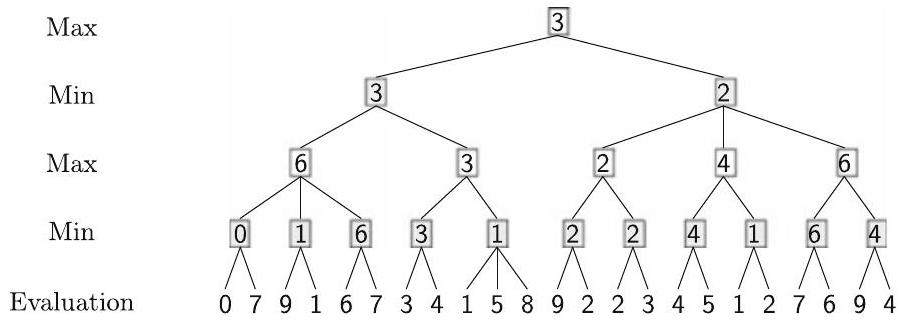
\includegraphics[max width=\textwidth, center]{2025_05_12_af19cd5e0d1b8a465ffeg-120(1)}
\end{enumerate}

Fig. 6.19 A minimax game tree with look-ahead of four half-moves\\
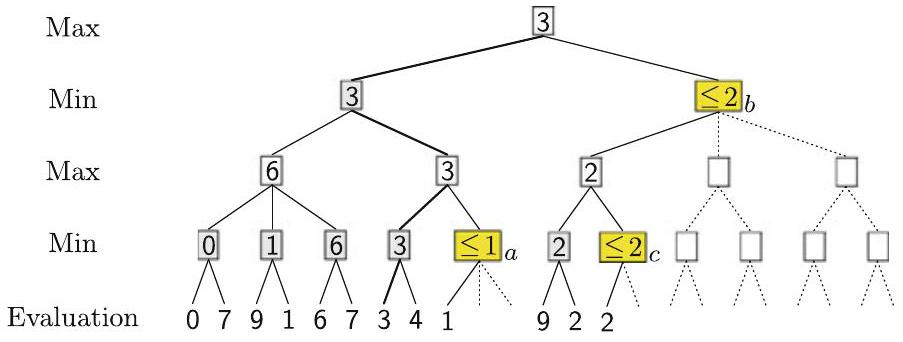
\includegraphics[max width=\textwidth, center]{2025_05_12_af19cd5e0d1b8a465ffeg-120}

Fig. 6.20 An alpha-beta game tree with look-ahead of four half-moves. The dotted portions of the tree are not traversed because they have no effect on the end result

\subsection*{6.4.2 Alpha-Beta-Pruning}
By switching between maximization and minimization, we can save ourselves a lot of work in some circumstances. Alpha-beta pruning works with depth-first search up to a preset depth limit. In this way the search tree is searched through from left to right. Like in minimax search, in the minimum nodes the minimum is generated from the minimum value of the successor nodes and in the maximum nodes likewise the maximum. In Fig. 6.20 this process is depicted for the tree from Fig. 6.19. At the node marked $a$, all other successors can be ignored after the first child is evaluated as the value 1 because the minimum is sure to be $\leq 1$. It could even become smaller still, but that is irrelevant since the maximum is already $\geq 3$ one level above. Regardless of how the evaluation of the remaining successors turns out, the maximum will keep the value 3 . Analogously the tree will be trimmed at node $b$. Since the first child of $b$ has the value 2 , the minimum to be generated for $b$ can only be less than or equal to 2 . But the maximum at the root node is already sure to be $\geq 3$. This cannot be changed by values $\leq 2$. Thus the remaining subtrees of $b$ can be pruned.

The same reasoning applies for the node $c$. However, the relevant maximum node is not the direct parent, but the root node. This can be generalized.

\begin{verbatim}
AlphaBetaMax(Node, $\alpha, \beta$ )
If DepthLimitReached(Node) Return(Rating(Node))
NewNodes = Successors(Node)
While NewNodes $\neq \varnothing$
    $\alpha=\operatorname{Maximum}(\alpha, \operatorname{AlphaBetaMin(First(NewNodes),~} \alpha, \beta)$ )
    If $\alpha \geq \beta$ Return $(\beta)$
    NewNodes $=\operatorname{Rest}($ NewNodes $)$
Return( $\alpha$ )
\end{verbatim}

AlphaBetaMin(Node, $\alpha, \beta$ )\\
If DepthLimitReached(Node) Return(Rating(Node))\\
NewNodes $=$ Successors(Node)\\
While NewNodes $\neq \emptyset$\\
$\beta=\operatorname{Minimum}(\beta$, AlphaBetaMax(First(NewNodes), $\alpha, \beta)$ )\\
If $\beta \leq \alpha$ Return $(\alpha)$\\
NewNodes $=$ Rest $($ NewNodes $)$\\
$\boldsymbol{\operatorname { R e t u r n }}(\boldsymbol{\beta})$

Fig. 6.21 The algorithm for alpha-beta search with the two functions AlphaBetaMin and AlphaBetaMax

\begin{itemize}
  \item At every leaf node the evaluation is calculated.
  \item For every maximum node the current largest child value is saved in $\alpha$.
  \item For every minimum node the current smallest child value is saved in $\beta$.
  \item If at a minimum node $k$ the current value $\beta \leq \alpha$, then the search under $k$ can end. Here $\alpha$ is the largest value of a maximum node in the path from the root to $k$.
  \item If at a maximum node $l$ the current value $\alpha \geq \beta$, then the search under $l$ can end. Here $\beta$ is the smallest value of a minimum node in the path from the root to $l$.
\end{itemize}

The algorithm given in Fig. 6.21 is an extension of depth-first search with two functions which are called in alternation. It uses the values defined above for $\alpha$ and $\beta$.

The initial alpha-beta pruning call is done with the command\\
AlphaBetaMax(RootNode, $-\infty, \infty$ ).

Complexity The computation time saved by alpha-beta pruning heavily depends on the order in which child nodes are traversed. In the worst case, alpha-beta\\
pruning does not offer any advantage. For a constant branching factor $b$ the number $n_{d}$ of leaf nodes to evaluate at depth $d$ is equal to

$$
n_{d}=b^{d}
$$

In the best case, when the successors of maximum nodes are descendingly sorted and the successors of minimum nodes are ascendingly sorted, the effective branching factor is reduced to $\sqrt{b}$. In chess this means a substantial reduction of the effective branching factor from 35 to about 6 . Then only

$$
n_{d}=\sqrt{b}^{d}=b^{d / 2}
$$

leaf nodes would be created. This means that the depth limit and thus also the search horizon are doubled with alpha-beta pruning. However, this is only true in the case of optimally sorted successors because the child nodes' ratings are unknown at the time when they are created. If the child nodes are randomly sorted, then the branching factor is reduced to $b^{3 / 4}$ and the number of leaf nodes to

$$
n_{d}=b^{\frac{3}{4} d} .
$$

With the same computing power a chess computer using alpha-beta pruning can, for example, compute eight half-moves ahead instead of six, with an effective branching factor of about 14. A thorough analysis with a derivation of these parameters can be found in [Pea84].

To double the search depth as mentioned above, we would need the child nodes to be optimally ordered, which is not the case in practice. Otherwise the search would be unnecessary. With a simple trick we can get a relatively good node ordering. We connect alpha-beta pruning with iterative deepening over the depth limit. Thus at every new depth limit we can access the ratings of all nodes of previous levels and order the successors at every branch. Thereby we reach an effective branching factor of roughly 7 to 8, which is not far from the theoretical optimum of $\sqrt{35}$ [Nil98].

\subsection*{6.4.3 Non-deterministic Games}
Minimax search can be generalized to all games with non-deterministic actions, such as backgammon. Each player rolls before his move, which is influenced by the result of the dice roll. In the game tree there are now therefore three types of levels in the sequence

Max, dice, Min, dice, ... ,\\[0pt]
where each dice roll node branches six ways. Because we cannot predict the value of the die, we average the values of all rolls and conduct the search as described with the average values from [RN10].

\subsection*{6.5 Heuristic Evaluation Functions}
How do we find a good heuristic evaluation function for the task of searching? Here there are fundamentally two approaches. The classical way uses the knowledge of human experts. The knowledge engineer is given the usually difficult task of formalizing the expert's implicit knowledge in the form of a computer program. We now want to show how this process can be simplified in the chess program example.

In the first step, experts are questioned about the most important factors in the selection of a move. Then it is attempted to quantify these factors. We obtain a list of relevant features or attributes. These are then (in the simplest case) combined into a linear evaluation function $B(s)$ for positions, which could look like:


\begin{align*}
B(s)= & a_{1} \cdot \text { material }+a_{2} \cdot \text { pawn_structure }+a_{3} \cdot \text { king_safety } \\
& +a_{4} \cdot \text { knight_in_center }+a_{5} \cdot \text { bishop_diagonal_coverage }+\cdots, \tag{6.3}
\end{align*}


where "material" is by far the most important feature and is calculated by

$$
\text { material }=\text { material(own_team) }- \text { material(opponent) }
$$

with

$$
\begin{aligned}
\text { material }(\text { team })= & \text { num_pawns }(\text { team }) \cdot 100+\text { num_knights }(\text { team }) \cdot 300 \\
& + \text { num_bishops }(\text { team }) \cdot 300+\text { num_rooks }(\text { team }) \cdot 500 \\
& + \text { num_queens }(\text { team }) \cdot 900
\end{aligned}
$$

Nearly all chess programs make a similar evaluation for material. However, there are big differences for all other features, which we will not go into here [Fra05, Lar00].

In the next step the weights $a_{i}$ of all features must be determined. These are set intuitively after discussion with experts, then changed after each game based on positive and negative experience. The fact that this optimization process is very expensive and furthermore that the linear combination of features is very limited suggests the use of machine learning.

\subsection*{6.5.1 Learning of Heuristics}
We now want to automatically optimize the weights $a_{i}$ of the evaluation function $B(\mathrm{~s})$ from (6.3). In this approach the expert is only asked about the relevant features $f_{1}(s), \ldots, f_{n}(s)$ for game state $s$. Then a machine learning process is used with the goal of finding an evaluation function that is as close to optimal as possible. We start with an initial pre-set evaluation function (determined by the learning process), and then let the chess program play. At the end of the game a rating is derived from the result (victory, defeat, or draw). Based on this rating, the evaluation function is\\
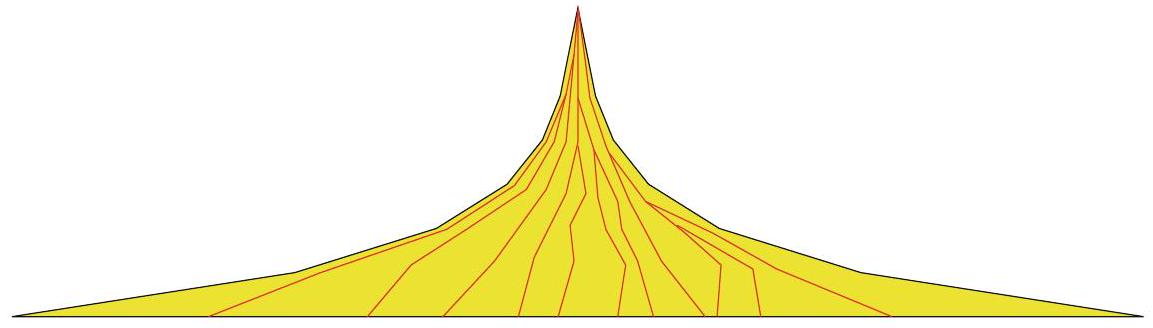
\includegraphics[max width=\textwidth, center]{2025_05_12_af19cd5e0d1b8a465ffeg-124}

Fig. 6.22 In this sketch of a search tree, several MCTS paths to leaf nodes are shown in red. Notice that only a small part of the tree is searched\\
changed with the goal of making fewer mistakes next time. In principle, the same thing that is done by the developer is now being taken care of automatically by the learning process.

As easy as this sounds, it is very difficult in practice. A central problem with improving the position rating based on won or lost matches is known today as the credit assignment problem. We do in fact have a rating at the end of the game, but no ratings for the individual moves. Thus the agent carries out many actions but does not receive any positive or negative feedback until the very end. How should it then assign this feedback to the many actions taken in the past? And how should it improve its actions in that case? The exciting field of reinforcement learning deals with these questions (see Chap. 10).

Monte Carlo tree search (MCTS) [KS06] works quite similarly. To improve the heuristic rating of a game state $s$, a random number of search tree branches starting from this state are either explored to the end and evaluated, or stopped at a certain depth and then the leaf nodes are evaluated heuristically. The evaluation $B(s)$ of state $s$ is given as the mean of all leaf node scores. The use of MCTS paths requires only a small part of the entire exponentially exploding tree to be searched. This is illustrated in Fig. 6.22. For many computer-simulated games, such as chess, this algorithm can be used to achieve better play for the same computational effort or to reduce computational effort for the same difficulty level [KS06]. This method was used together with machine learning algorithms in 2016 by the program AlphaGo, described in Sect. 10.10, which was the first Go program to defeat world-class human players [SHM ${ }^{+} 16$ ].

\subsection*{6.6 State of the Art}
For evaluation of the quality of the heuristic search processes, I would like to repeat Elaine Rich's definition [Ric83]:

Artificial Intelligence is the study of how to make computers do things at which, at the moment, people are better.

There is hardly a better suited test for deciding whether a computer program is intelligent as the direct comparison of computer and human in a game like chess, checkers, backgammon or Go.

In 1950, Claude Shannon, Konrad Zuse, and John von Neumann introduced the first chess programs, which, however, could either not be implemented or would take a great deal of time to implement. Just a few years later, in 1955, Arthur Samuel wrote a program that played checkers and could improve its own parameters through a simple learning process. To do this he used the first programmable logic computer, the IBM 701. Compared to the chess computers of today, however, it had access to a large number of archived games, for which every individual move had been rated by experts. Thus the program improved its evaluation function. To achieve further improvements, Samuel had his program play against itself. He solved the credit assignment problem in a simple manner. For each individual position during a game it compares the evaluation by the function $B(s)$ with the one calculated by alpha-beta pruning and changes $B(s)$ accordingly. In 1961 his checkers program beat the fourth-best checkers player in the USA. With this ground-breaking work, Samuel was surely nearly 30 years ahead of his time.

Only at the beginning of the nineties, as reinforcement learning emerged, did Gerald Tersauro build a learning backgammon program named TD-Gammon, which played at the world champion level (see Chap. 10).

\subsection*{6.6.1 Chess}
Today many chess programs exist that play above grandmaster level. The breakthrough came in 1997, as IBM's Deep Blue defeated the chess world champion Gary Kasparov with a score of 3.5 games to 2.5. Deep Blue could on average compute 12 half-moves ahead with alpha-beta pruning and heuristic position evaluation.

Around the year 2005 one of the most powerful chess computers was Hydra, a parallel computer owned by a company in the United Arab Emirates. The software was developed by the scientists Christian Donninger (Austria) and Ulf Lorenz (Germany), as well as the German chess grand champion Christopher Lutz. Hydra uses 64 parallel Xeon processors with about 3 GHz computing power and 1 GByte memory each. For the position evaluation function each processor has an FPGA (field programmable gate array) co-processor. Thereby it becomes possible to evaluate 200 million positions per second even with an expensive evaluation function.

With this technology Hydra can on average compute about 18 moves ahead. In special, critical situations the search horizon can even be stretched out to 40 half-moves. Clearly this kind of horizon is beyond what even grand champions can do, for Hydra often makes moves which grand champions cannot comprehend, but which in the end lead to victory. In 2005 Hydra defeated seventh ranked grandmaster Michael Adams with 5.5-0.5 games.

Hydra uses little special textbook knowledge about chess, rather alpha-beta search with relatively general, well-known heuristics and a good hand-coded\\
position evaluation. In particular, Hydra is not capable of learning. Improvements are carried out between games by the developers. As a consequence, Hydra was soon outperformed by machines that used smart learning algorithms rather than expensive hardware.

In 2009 the system Pocket Fritz 4, running on a PDA, won the Copa Mercosur chess tournament in Buenos Aires with nine wins and one draw against 10 excellent human chess players, three of them grandmasters. Even though not much information about the internal structure of the software is available, this chess machine represents a trend away from raw computing power toward more intelligence. This machine plays at grandmaster level, and is comparable to, if not better than Hydra. According to Pocket Fritz developer Stanislav Tsukrov [Wik13], Pocket Fritz with its chess search engine HIARCS 13 searches less than 20,000 positions per second, which is slower than Hydra by a factor of about 10,000 . This leads to the conclusion that HIARCS 13 definitely uses better heuristics to decrease the effective branching factor than Hydra and can thus well be called more intelligent than Hydra. By the way, HIARCS is a short hand for Higher Intelligence Auto Response Chess System.

\subsection*{6.6.2 Go}
Even though today no human stands a chance against the best chess computers, there are still many challenges for AI. For example Go. In this ancient Japanese game, played on a square board of 361 spaces with 181 white and 180 black stones, the effective branching factor is about 250 . After 8 half-moves there are already $1.5 \cdot 10^{19}$ possible positions. Given this complexity, none of the classic, well-known game tree search algorithms have a chance against a good human Go player. Yet in the most recent previous edition of this book, it was stated that:

\begin{displayquote}
The experts agree that "truly intelligent" algorithms are needed here. Combinatoric enumeration of all possibilities is the wrong approach. Rather, procedures are needed that recognize patterns on the board, track gradual developments, and make rapid "intuitive" decisions. Similar to object recognition in complex images, we humans are still far superior to today's computer programs. We process the image as a whole in a highly parallel manner, whereas the computer processes the millions of pixels successively and has great difficulty recognizing the essentials in the abundance of pixels. The program "The Many Faces of Go" recognizes 1100 different patterns and knows 200 different playing strategies. All Go programs, however, still have great difficulty recognizing whether a group of stones is dead or alive, or where in between to classify them.
\end{displayquote}

This statement is now obsolete. In January of 2016, Google [SHM+ 16] and Facebook [TZ16] published the breakthrough concurrently. That same month, the program AlphaGo, developed and presented in $\left[\mathrm{SHM}^{+} 16\right]$ by Google DeepMind, defeated European Go champion Fan Hui 5:0. Two months later, Korean player Lee Sedol, one of the best in the world, was defeated 4:1. Deep Learning for pattern recognition (see Sect. 9.7), reinforcement learning (see Chap. 10) and Monte Carlo tree search (MCTS, see Sect. 6.5.1) lead to this successful result.

The program plays hundreds of thousands of games against itself and uses the results (win, loss, draw) to learn the best possible heuristic score for a given position. Monte Carlo tree search is used as a replacement for Minimax search, which is not suitable for Go. In Sect. 10.10, after we have gained familiarity with the necessary learning algorithms, we will introduce AlphaGo.

\subsection*{6.7 Exercises}
\section*{Exercise 6.1}
(a) Prove Theorem 6.1 on page 96, in other words, prove that for a tree with large constant branching factor $b$, almost all nodes are on the last level at depth $d$.\\
(b) Show that this is not always true when the effective branching factor is large and not constant.

\section*{Exercise 6.2}
(a) Calculate the average branching factor for the 8-puzzle without a check for cycles. The average branching factor is the branching factor that a tree with an equal number of nodes on the last level, constant branching factor, and equal depth would have.\\
(b) Calculate the average branching factor for the 8-puzzle for uninformed search while avoiding cycles of length 2 .

\section*{Exercise 6.3}
(a) What is the difference between the average and the effective branching factor (Definition 6.2 on page 95)?\\
(b) Why is the effective branching factor better suited to analysis and comparison of the computation time of search algorithms than the average branching factor?\\
(c) Show that for a heavily branching tree with $n$ nodes and depth $d$ the effective branching factor $\bar{b}$ is approximately equal to the average branching factor and thus equal to $\sqrt[d]{n}$.

\section*{Exercise 6.4}
(a) Calculate the size of the state space for the 8-puzzle, for the analogous 3 -puzzle ( $2 \times 2$-matrix), as well as for the 15 -puzzle ( $4 \times 4$-matrix).\\
(b) Prove that the state graph consisting of the states (nodes) and the actions (edges) for the 3-puzzle falls into two connected sub-graphs, between which there are no connections.

Exercise 6.5 With breadth-first search for the 8-puzzle, find a path (manually) from the starting node

\begin{center}
\begin{tabular}{|l|l|l|}
\hline
1 &  & 3 \\
\hline
4 & 2 & 6 \\
\hline
7 & 5 & 8 \\
\hline
\end{tabular}
\end{center} to the goal node \begin{tabular}{|l|l|l|l|}
\hline
1 & 2 & 3 \\
\hline
4 & 5 & 6 \\
\hline
7 & 8 &  \\
\hline
\end{tabular}

\section*{\#> Exercise 6.6}
(a) Program breadth-first search, depth-first search, and iterative deepening in the language of your choice and test them on the 8-puzzle example.\\
(b) Why does it make little sense to use depth-first search on the 8-puzzle?

\section*{Exercise 6.7}
(a) Show that breadth-first search given constant cost for all actions is guaranteed to find the shortest solution.\\
(b) Show that this is not the case for varying costs.

Exercise 6.8 The predecessors of all nodes must be stored to check for cycles during depth-first search.\\
(a) For depth first search develop a data structure (not a hash table) that is as efficient as possible for storing all nodes in the search path of a search tree.\\
(b) For constant branching factor $b$ and depth $d$, give a formula for the storage space needed by depth-first search with and without storing predecessors.\\
(c) Show that for large $b$ and $d$, we have $\sum_{k=0}^{d} k \cdot b^{k} \approx d \cdot b^{d}$.

Exercise 6.9 Using $A^{\star}$ search for the 8-puzzle, search (manually) for a path from\\
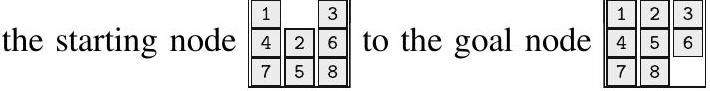
\includegraphics[max width=\textwidth, center]{2025_05_12_af19cd5e0d1b8a465ffeg-128}\\
(a) using the heuristic $h_{1}$ (Sect. 6.3.4).\\
(b) using the heuristic $h_{2}$ (Sect. 6.3.4).

Exercise 6.10 Construct the $A^{\star}$ search tree for the city graph from Fig. 6.14 on page 106 and use the flying distance to Ulm as the heuristic. Start in Bern with Ulm as the destination. Take care that each city only appears once per path.

\section*{Exercise 6.11}
(a) Show that the triangle inequality is valid for shortest distances on maps.\\
(b) Using an example, show that it is not always the case that the triangle inequality holds for direct neighbor nodes $x$ and $y$, where the distance is $d(x, y)$. That is, it is not the case that $d(x, y) \leq d(x, z)+d(z, y)$.\\
$\rightarrow$ Exercise 6.12 Program $A^{\star}$ search in the programming language of your choice using the heuristics $h_{1}$ and $h_{2}$ and test these on the 8 -puzzle example.

\begin{itemize}
  \item Exercise 6.13 Give a heuristic evaluation function for states with which HeuristicSearch can be implemented as depth-first search, and one for a breadth-first search implementation.
\end{itemize}

Exercise 6.14 What is the relationship between the picture of the couple at the canyon from Fig. 6.13 on page 105 and admissible heuristics?

Exercise 6.15 Show that the heuristics $h_{1}$ and $h_{2}$ for the 8-puzzle from Sect. 6.3.4 are admissible.

\section*{Exercise 6.16}
(a) The search tree for a two-player game is given in Fig. 6.23 with the ratings of all leaf nodes. Use minimax search with $\alpha-\beta$ pruning from left to right. Cross out all nodes that are not visited and give the optimal resulting rating for each inner node. Mark the chosen path.\\[0pt]
(b) Test yourself using P. Winston's applet [Win].\\
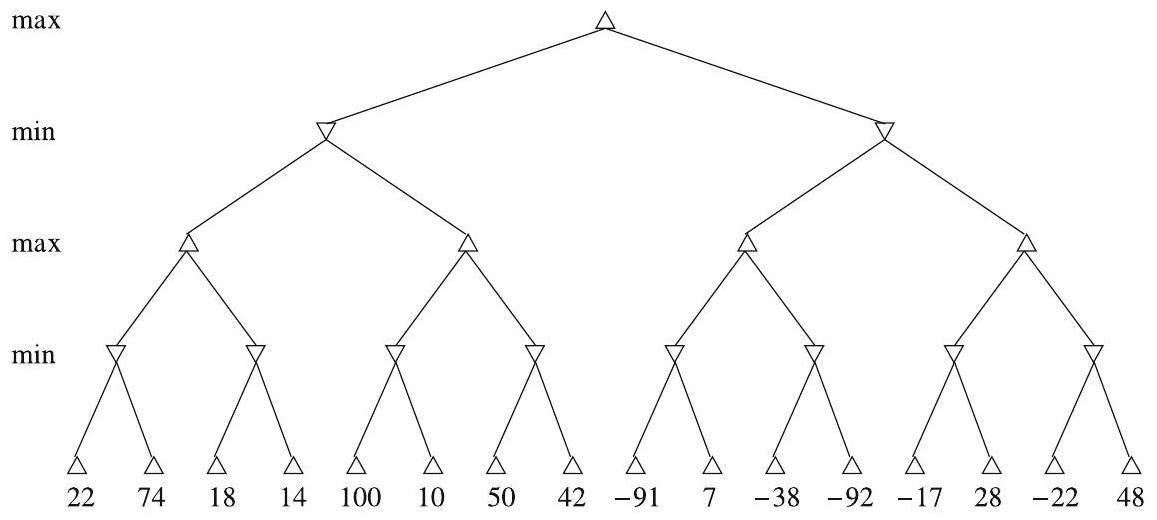
\includegraphics[max width=\textwidth, center]{2025_05_12_af19cd5e0d1b8a465ffeg-129}

Fig. 6.23 Minimax search tree

\section*{Reasoning with Uncertainty}
\section*{7}
We have already shown in Chap. 4 with the Tweety problem that two-value logic leads to problems in everyday reasoning. In this example, the statements Tweety is a penguin, Penguins are birds, and All birds can fly lead to the (semantically incorrect) inference Tweety can fly. Probability theory provides a language in which we can formalize the statement Nearly all birds can fly and carry out inferences on it. Probability theory is a proven method we can use here because the uncertainty about whether birds can fly can be modeled well by a probability value. We will show, that statements such as $99 \%$ of all birds can fly, together with probabilistic logic, lead to correct inferences.

Reasoning under uncertainty with limited resources plays a big role in everyday situations and also in many technical applications of AI. In these areas heuristic processes are very important, as we have already discussed in Chap. 6. For example, we use heuristic techniques when looking for a parking space in city traffic. Heuristics alone are often not enough, especially when a quick decision is needed given incomplete knowledge, as shown in the following example. A pedestrian crosses the street and an auto quickly approaches. To prevent a serious accident, the pedestrian must react quickly. He is not capable of worrying about complete information about the state of the world, which he would need for the search algorithms discussed in Chap. 6. He must therefore come to an optimal decision under the given constraints (little time and little, potentially uncertain knowledge). If he thinks too long, it will be dangerous. In this and many similar situations (see Fig. 7.1 on page 126), a method for reasoning with uncertain and incomplete knowledge is needed.

We want to investigate the various possibilities of reasoning under uncertainty in a simple medical diagnosis example. If a patient experiences pain in the right lower abdomen and a raised white blood cell (leukocyte) count, this raises the suspicion that it might be appendicitis. We model this relationship using propositional logic with the formula

Stomach pain right lower $\wedge$ Leukocytes $>10000 \rightarrow$ Appendicitis\\
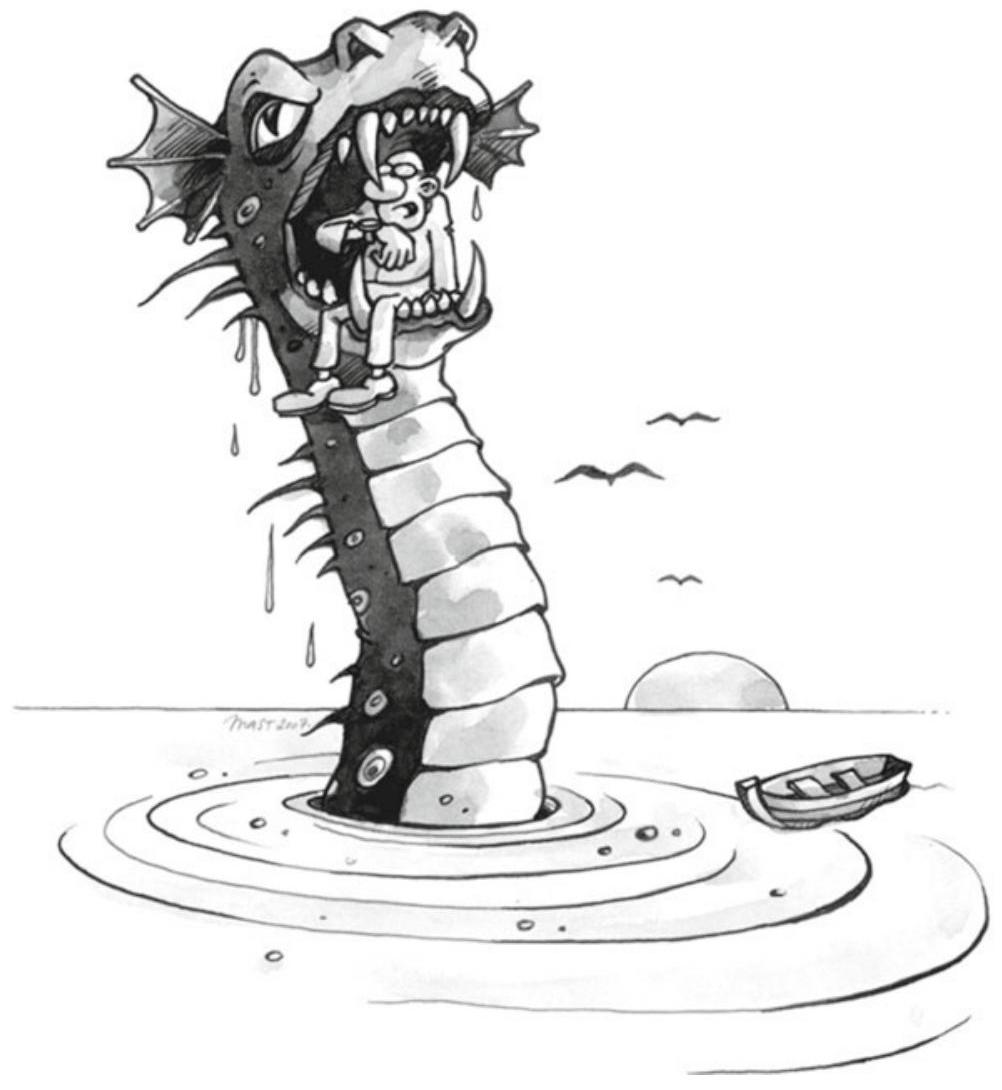
\includegraphics[max width=\textwidth, center]{2025_05_12_af19cd5e0d1b8a465ffeg-131}

Fig. 7.1 "Let's just sit back and think about what to do!"\\
If we then know that

$$
\text { Stomach pain right lower } \wedge \text { Leukocytes }>10000
$$

is true, then we can use modus ponens to derive Appendicitis. This model is clearly too coarse. In 1976, Shortliffe and Buchanan recognized this when building their medical expert system MYCIN [Sho76]. They developed a calculus using so-called certainty factors, which allowed the certainty of facts and rules to be represented. A rule $A \rightarrow B$ is assigned a certainty factor $\beta$. The semantic of a rule $A \rightarrow{ }_{\beta} B$ is defined via the conditional probability $P(B \mid A)=\beta$. In the above example, the rule could then read

$$
\text { Stomach pain right lower } \wedge \text { Leukocytes }>10000 \rightarrow_{0.6} \text { Appendicitis. }
$$

For reasoning with this kind of formulas, they used a calculus for connecting the factors of rules. It turned out, however, that with this calculus inconsistent results could be derived.

As discussed in Chap. 4, there were also attempts to solve this problem by using non-monotonic logic and default logic, which, however, were unsuccessful in the end. The Dempster-Schäfer theory assigns a belief function $\operatorname{Bel}(A)$ to a logical proposition $A$, whose value gives the degree of evidence for the truth of $A$. But even this formalism has weaknesses, which is shown in [Pea88] using a variant of the Tweety example. Even fuzzy logic, which above all is successful in control theory, demonstrates considerable weaknesses when reasoning under uncertainty in more complex applications [Elk93].

Since about the mid-1980s, probability theory has had more and more influence in AI [Pea88, Che85, Whi96, Jen01]. In the field of reasoning with Bayesian networks, or subjective probability, it has secured itself a firm place among successful AI techniques. Rather than implication as it is known in logic (material implication), conditional probability is used here, which models everyday causal reasoning significantly better. Reasoning with probability profits heavily from the fact that probability theory is a hundreds of years old, well-established branch of mathematics.

In this chapter we will select an elegant, but for an instruction book somewhat unusual, entry point into this field. After a short introduction to the most important foundations needed here for reasoning with probability, we will begin with a simple, but important example for reasoning with uncertain and incomplete knowledge. In a quite natural, almost compelling way, we will be led to the method of maximum entropy (MaxEnt). Then we will show the usefulness of this method in practice using the medical expert system lexmed. Finally we will introduce the now widespread reasoning with Bayesian networks, and show the relationship between the two methods.

\subsection*{7.1 Computing with Probabilities}
The reader who is familiar with probability theory can skip this section. For everyone else we will give a quick ramp-up and recommend a few appropriate textbooks such as [Ros09, FPP07].

Probability is especially well-suited for modeling reasoning under uncertainty. One reason for this is that probabilities are intuitively easy to interpret, which can be seen in the following elementary example.

Example 7.1 For a single roll of a gaming die (experiment), the probability of the event "rolling a six" equals $1 / 6$, whereas the probability of the occurrence "rolling an odd number" is equal to $1 / 2$.

Definition 7.1 Let $\Omega$ be the finite set of events for an experiment. Each event $\omega \in \Omega$ represents a possible outcome of the experiment. If these events $w_{i} \in \Omega$ mutually exclude each other, but cover all possible outcomes of the attempt, then they are called elementary events.

Example 7.2 For a single roll of one gaming die

$$
\Omega=\{1,2,3,4,5,6\}
$$

because no two of these events can happen simultaneously. Rolling an even number ( $\{2,4,6\}$ ) is therefore not an elementary event, nor is rolling a number smaller than five ( $\{1,2,3,4\}$ ) because $\{2,4,6\} \cap\{1,2,3,4\}=\{2,4\} \neq \emptyset$.

Given two events $A$ and $B, A \cup B$ is also an event. $\Omega$ itself is denoted the certain event, and the empty set $\emptyset$ the impossible event.

In the following we will use the propositional logic notation for set operations. That is, for the set $A \cap B$ we write $A \wedge B$. This is not only a syntactic transformation, rather it is also semantically correct because the intersection of two sets is defined as

$$
x \in A \cap B \Leftrightarrow x \in A \wedge x \in B .
$$

Because this is the semantic of $A \wedge B$, we can and will use this notation. This is also true for the other set operations union and complement, and we will, as shown in the following table, use the propositional logic notation for them as well.

\begin{center}
\begin{tabular}{|l|l|l|}
\hline
Set notation & Propositional logic & Description \\
\hline
$A \cap B$ & $A \wedge B$ & intersection / and \\
\hline
$A \cup B$ & $A \vee B$ & union / or \\
\hline
$\bar{A}$ & $\neg A$ & complement / negation \\
\hline
$\Omega$ & $t$ & certain event / true \\
\hline
$\emptyset$ & $f$ & impossible event / false \\
\hline
\end{tabular}
\end{center}

The variables used here (for example $A, B$, etc.) are called random variables in probability theory. We will only use discrete chance variables with finite domains here. The variable face\_number for a dice roll is discrete with the values $1,2,3,4$, 5,6 . The probability of rolling a five or a six is equal to $1 / 3$. This can be described by

$$
P(\text { face_number } \in\{5,6\})=P(\text { face_number }=5 \vee \text { face_number }=6)=1 / 3 .
$$

The concept of probability is supposed to give us a description as objective as possible of our "belief" or "conviction" about the outcome of an experiment. All numbers in the interval $[0,1]$ should be possible, where 0 is the probability of the impossible event and 1 the probability of the certain event. We come to this from the following definition.

Definition 7.2 Let $\Omega=\left\{\omega_{1}, \omega_{2}, \ldots, \omega_{n}\right\}$ be finite. There is no preferred elementary event, which means that we assume a symmetry related to the frequency of how often each elementary event appears. The probability $P(A)$ of the event $A$ is then

$$
P(A)=\frac{|A|}{|\Omega|}=\frac{\text { Number of favorable cases for } A}{\text { Number of possible cases }} .
$$

It follows immediately that every elementary event has the probability $1 /|\Omega|$. The requirement that elementary events have equal probability is called the Laplace assumption and the probabilities calculated thereby are called Laplace probabilities. This definition hits its limit when the number of elementary events becomes infinite. Because we are only looking at finite event spaces here, though, this does not present a problem. To describe events we use variables with the appropriate number of values. For example, a variable eye\_color can take on the values green, blue, brown. eye\_color = blue then describes an event because we are dealing with a proposition with the truth values $t$ or $f$. For binary (boolean) variables, the variable itself is already a proposition. Here it is enough, for example, to write $P$ (JohnCalls) instead of $P($ JohnCalls $=t)$.

Example 7.3 By this definition, the probability of rolling an even number is

$$
P(\text { face_number } \in\{2,4,6\})=\frac{|\{2,4,6\}|}{|\{1,2,3,4,5,6\}|}=\frac{3}{6}=\frac{1}{2} .
$$

The following important rules follow directly from the definition.

\section*{Theorem 7.1}
\begin{enumerate}
  \item $P(\Omega)=1$.
  \item $P(\emptyset)=0$, which means that the impossible event has a probability of 0 .
  \item For pairwise exclusive events $A$ and $B$ it is true that $P(A \vee B)=P(A)+P(B)$.
  \item For two complementary events $A$ and $\neg A$ it is true that $P(A)+P(\neg A)=1$.
  \item For arbitrary events $A$ and $B$ it is true that $P(A \vee B)=P(A)+P(B)-$ $P(A \wedge B)$.
  \item For $A \subseteq B$ it is true that $P(A) \leq P(B)$.
  \item If $A_{1}, \ldots, A_{n}$ are the elementary events, then $\sum_{i=1}^{n} P\left(A_{i}\right)=1$ (normalization condition).
\end{enumerate}

The expression $P(A \wedge B)$ or equivalently $P(A, B)$ stands for the probability of the events $A \wedge B$. We are often interested in the probabilities of all elementary events, that is, of all combinations of all values of the variables $A$ and $B$. For the binary variables $A$ and $B$ these are $P(A, B), P(A, \neg B), P(\neg A, B), P(\neg A, \neg B)$. We call the vector

$$
(P(A, B), P(A, \neg B), P(\neg A, B), P(\neg A, \neg B))
$$

consisting of these four values a distribution or joint probability distribution of the variables $A$ and $B$. A shorthand for this is $\boldsymbol{P}(A, B)$. The distribution in the case of two variables can be nicely visualized in the form of a table (matrix), represented as follows:

\begin{center}
\begin{tabular}{lll}
\hline
$\boldsymbol{P}(A, B)$ & $B=w$ & $B=f$ \\
\hline
$A=w$ & $P(A, B)$ & $P(A, \neg B)$ \\
\hline
$A=f$ & $P(\neg A, B)$ & $P(\neg A, \neg B)$ \\
\hline
\end{tabular}
\end{center}

For the $d$ variables $X_{1}, \ldots, X_{d}$ with $n$ values each, the distribution has the values $P\left(X_{1}=x_{1}, \ldots, X_{d}=x_{d}\right)$ and $x_{1}, \ldots, x_{d}$, each of which take on $n$ different values. The distribution can therefore be represented as a $d$-dimensional matrix with a total of $n^{d}$ elements. Due to the normalization condition from Theorem 7.1 on page 129, however, one of these $n^{d}$ values is redundant and the distribution is characterized by $n^{d}-1$ unique values.

\subsection*{7.1.1 Conditional Probability}
Example 7.4 On Landsdowne street in Boston, the speed of 100 vehicles is measured. For each measurement it is also noted whether the driver is a student. The results are

\begin{center}
\begin{tabular}{|l|l|l|}
\hline
Event & Frequency & Relative frequency \\
\hline
Vehicle observed & 100 & 1 \\
\hline
Driver is a student ( $S$ ) & 30 & 0.3 \\
\hline
Speed too high ( $G$ ) & 10 & 0.1 \\
\hline
Driver is a student and speeding ( $S \wedge G$ ) & 5 & 0.05 \\
\hline
\end{tabular}
\end{center}

We pose the question: Do students speed more frequently than the average person, or than non-students? ${ }^{1}$

\footnotetext{${ }^{1}$ The computed probabilities can only be used for continued propositions if the measured sample (100 vehicles) is representative. Otherwise only propositions about the observed 100 vehicles can be made.
}The answer is given by the probability

$$
P(G \mid S)=\frac{\mid \text { Driver is a student and speeding } \mid}{\mid \text { Driver is a student } \mid}=\frac{5}{30}=\frac{1}{6} \approx 0.17
$$

for speeding under the condition that the driver is a student. This is obviously different from the a priori probability $P(G)=0.1$ for speeding. For the a priori probability, the event space is not limited by additional conditions.

Definition 7.3 For two events $A$ and $B$, the probability $P(A \mid B)$ for $A$ under the condition $B$ (conditional probability) is defined by

$$
P(A \mid B)=\frac{P(A \wedge B)}{P(B)} .
$$

In Example 7.4 we see that in the case of a finite event space, the conditional probability $P(A \mid B)$ can be understood as the probability of $A \wedge B$ when we only look at the event $B$, that is, as

$$
P(A \mid B)=\frac{|A \wedge B|}{|B|} .
$$

This formula can be easily derived using Definition 7.2 on page 129

$$
P(A \mid B)=\frac{P(A \wedge B)}{P(B)}=\frac{\frac{|A \wedge B|}{|\Omega|}}{\frac{|B|}{|\Omega|}}=\frac{|A \wedge B|}{|B|} .
$$

Definition 7.4 If, for two events $A$ and $B$,

$$
P(A \mid B)=P(A),
$$

then these events are called independent.

Thus $A$ and $B$ are independent if the probability of the event $A$ is not influenced by the event $B$.

Theorem 7.2 For independent events $A$ and $B$, it follows from the definition that

$$
P(A \wedge B)=P(A) \cdot P(B)
$$

Example 7.5 For a roll of two dice, the probability of rolling two sixes is $1 / 36$ if the two dice are independent because

$$
P\left(D_{1}=6 \wedge D_{2}=6\right)=P\left(D_{1}=6\right) \cdot P\left(D_{2}=6\right)=\frac{1}{6} \cdot \frac{1}{6}=\frac{1}{36}
$$

where the first equation is only true when the two dice are independent. If for example by some magic power die 2 is always the same as die 1 , then

$$
P\left(D_{1}=6 \wedge D_{2}=6\right)=\frac{1}{6}
$$

\section*{Chain Rule}
Solving the definition of conditional probability for $P(A \wedge B)$ results in the so-called product rule

$$
P(A \wedge B)=P(A \mid B) P(B),
$$

which we immediately generalize for the case of $n$ variables. By repeated application of the above rule we obtain the chain rule


\begin{align*}
\boldsymbol{P}\left(X_{1}\right. & \left., \ldots, X_{n}\right) \\
& =\boldsymbol{P}\left(X_{n} \mid X_{1}, \ldots, X_{n-1}\right) \cdot \boldsymbol{P}\left(X_{1}, \ldots, X_{n-1}\right) \\
& =\boldsymbol{P}\left(X_{n} \mid X_{1}, \ldots, X_{n-1}\right) \cdot \boldsymbol{P}\left(X_{n-1} \mid X_{1}, \ldots, X_{n-2}\right) \cdot \boldsymbol{P}\left(X_{1}, \ldots, X_{n-2}\right) \\
& =\boldsymbol{P}\left(X_{n} \mid X_{1}, \ldots, X_{n-1}\right) \cdot \boldsymbol{P}\left(X_{n-1} \mid X_{1}, \ldots, X_{n-2}\right) \cdot \ldots \cdot \boldsymbol{P}\left(X_{n} \mid X_{1}\right) \cdot \boldsymbol{P}\left(X_{1}\right) \\
& =\prod_{i=1}^{n} \boldsymbol{P}\left(X_{n} \mid X_{1}, \ldots, X_{i-1}\right) \tag{7.1}
\end{align*}


with which we can represent a distribution as a product of conditional probabilities. Because the chain rule holds for all values of the variables $X_{1}, \ldots, X_{n}$, it has been formulated for the distribution using the symbol $\boldsymbol{P}$.

\section*{Marginalization}
Because $A \Leftrightarrow(A \wedge B) \vee(A \wedge \neg B)$ is true for binary variables $A$ and $B$

$$
P(A)=P((A \wedge B) \vee(A \wedge \neg B))=P(A \wedge B)+P(A \wedge \neg B) .
$$

By summation over the two values of $B$, the variable $B$ is eliminated. Analogously, for arbitrary variables $X_{1}, \ldots, X_{d}$, a variable, for example $X_{d}$, can be eliminated by summation over all of their variables and we get

$$
P\left(X_{1}=x_{1}, \ldots, X_{d-1}=x_{d-1}\right)=\sum_{x_{d}} P\left(X_{1}=x_{1}, \ldots, X_{d-1}=x_{d-1}, X_{d}=x_{d}\right) .
$$

The application of this formula is called marginalization. This summation can continue with the variables $X_{1}, \ldots, X_{d-1}$ until just one variable is left. Marginalization can also be applied to the distribution $\boldsymbol{P}\left(X_{1}, \ldots, X_{d}\right)$. The resulting distribution $\boldsymbol{P}\left(X_{1}, \ldots, X_{d-1}\right)$ is called the marginal distribution. It is comparable to the projection of a rectangular cuboid on a flat surface. Here the three-dimensional object is drawn on the edge or "margin" of the cuboid, i.e. on a two-dimensional set. In both cases the dimensionality is reduced by one.

Example 7.6 We observe the set of all patients who come to the doctor with acute stomach pain. For each patient the leukocyte value is measured, which is a metric for the relative abundance of white blood cells in the blood. We define the variable Leuko, which is true if and only if the leukocyte value is greater than 10,000 . This indicates an infection in the body. Otherwise we define the variable App, which tells us whether the patient has appendicitis, that is, an infected appendix. The distribution $\boldsymbol{P}($ App, Leuko $)$ of these two variables is given in the following table:

\begin{center}
\begin{tabular}{llll}
\hline
$\boldsymbol{P}($ App, Leuko $)$ & $A p p$ & $\neg A p p$ & Total \\
\hline
Leuko & 0.23 & 0.31 & 0.54 \\
\hline
$\neg$ Leuko & 0.05 & 0.41 & 0.46 \\
\hline
Total & 0.28 & 0.72 & 1 \\
\hline
\end{tabular}
\end{center}

In the last row the sum over the rows is given, and in the last column the sum of the columns is given. These sums are arrived at by marginalization. For example, we read off

$$
P(\text { Leuko })=P(\text { App }, \text { Leuko })+P(\neg \text { App }, \text { Leuko })=0.54 .
$$

The given distribution $\boldsymbol{P}$ (App, Leuko) could come from a survey of German doctors, for example. From it we can then calculate the conditional probability

$$
P(\text { Leuko } \mid A p p)=\frac{P(\text { Leuko }, A p p)}{P(A p p)}=0.82
$$

which tells us that about $82 \%$ of all appendicitis cases lead to a high leukocyte value. Values like this are published in medical literature. However, the conditional\\
probability $P(A p p \mid$ Leuko $)$, which would actually be much more helpful for diagnosing appendicitis, is not published. To understand this, we will first derive a simple, but very important formula.

\section*{Bayes' Theorem}
Swapping $A$ and $B$ in Definition 7.3 yields

$$
P(A \mid B)=\frac{P(A \wedge B)}{P(B)} \quad \text { and } \quad P(B \mid A)=\frac{P(A \wedge B)}{P(A)}
$$

By solving both equations for $P(A \wedge B)$ and equating them we obtain Bayes’ theorem


\begin{equation*}
P(A \mid B)=\frac{P(B \mid A) \cdot P(A)}{P(B)} \tag{7.2}
\end{equation*}


whose relevance to many applications we will illustrate using three examples. First we apply it to the appendicitis example and obtain

\section*{Example 7.7}

\begin{equation*}
P(A p p \mid \text { Leuko })=\frac{P(\text { Leuko } \mid A p p) \cdot P(A p p)}{P(\text { Leuko })}=\frac{0.82 \cdot 0.28}{0.54}=0.43 . \tag{7.3}
\end{equation*}


Why then is $P($ Leuko $\mid A p p)$ published, but not $P($ App $\mid$ Leuko $)$ ?\\
Assuming that appendicitis affects the biology of all humans the same, regardless of ethnicity, $P($ Leuko $\mid A p p)$ is a universal value that is valid worldwide. In Equation 7.3 we see that $P(A p p \mid$ Leuko $)$ is not universal, for this value is influenced by the a priori probabilities $P(A p p)$ and $P($ Leuko $)$. Each of these can vary according to one's life circumstances. For example, $P($ Leuko $)$ is dependent on whether a population has a high or low rate of exposure to infectious diseases. In the tropics, this value can differ significantly from that of cold regions. Bayes' theorem, however, makes it easy for us to take the universally valid value $P($ Leuko $\mid A p p)$, and compute $P($ App $\mid$ Leuko $)$ which is useful for diagnosis.

Before we dive deeper into this example and build a medical expert system for appendicitis in Sect. 7.3 let us first apply Bayes' theorem to another interesting medical example.

Example 7.8 In cancer diagnosis, so-called tumor markers are often measured. One example of this is the use of the tumor marker PSA (prostate specific antigen) for the diagnosis of prostate cancer ( $\mathrm{PCa}=$ prostate cancer) in men. Assuming that no further tests for PCa have been conducted, the test is considered positive, that is, there is suspected PCa , if the concentration of PSA reaches a level at or above $4 \mathrm{ng} / \mathrm{ml}$. If this occurs, the probability $P(C \mid$ pos $)$ of PCa is of interest to the patient.

The binary variable $C$ is true if the patient has PCa , and pos represents a PSA value $\geq 4 \mathrm{ng} / \mathrm{ml}$. Let us now compute the $P(C \mid$ pos $)$. For reasons similar to those mentioned for appendicitis diagnosis, this value is not reported. Instead, researchers publish the sensitivity $P(p o s \mid C)$ and the specificity $P(n e g \mid \neg C)$ of the test. ${ }^{2}$ According to [HL04], for a sensitivity of 0.95, the specificity can be at most 0.25, which is why we proceed from $P($ pos $\mid C)=0.95$ and $P($ neg $\mid \neg C)=0.25$ below. We apply Bayes' theorem and obtain

$$
\begin{aligned}
P(C \mid p o s) & =\frac{P(p o s \mid C) \cdot P(C)}{P(p o s)}=\frac{P(p o s \mid C) \cdot P(C)}{P(p o s \mid C) \cdot P(C)+P(p o s \mid \neg C) \cdot P(\neg C)} \\
& =\frac{0.95 \cdot 0.0021}{0.95 \cdot 0.0021+\mathbf{0 . 7 5} \cdot 0.99679}=\frac{0.95 \cdot 0.0021}{0.75}=0.0027
\end{aligned}
$$

Here we use $P($ pos $\mid \neg C)=1-P($ neg $\mid \neg C)=1-0.25=0.75$ and $P(C)=$ $0.0021=0.21 \%$ as the a priori probability of PCa during one year. ${ }^{3}$ It makes sense to assume that the PSA test is done once per year. This result is somewhat surprising from the patient's perspective because the probability of PCa after a positive test is, at $0.27 \%$, only marginally higher than the probability of $0.21 \%$ for PCa for a 55-year-old man. Thus, a PSA value of just over $4 \mathrm{ng} / \mathrm{ml}$ is definitively no reason for the patient to panic. At most it is used as a basis for further examinations, such as biopsy or MRI, leading if necessary to radiation and surgery. The situation is similar for many other tumor markers such as those for colorectal cancer or breast cancer diagnosis by mammography.

The cause of this problem is the very low specificity $P(n e g \mid \neg C)=0.25$, which leads to $75 \%$ of healthy patients (without PCa ) getting a false-positive test result and consequently undergoing unnecessary examinations. Because of this, PSA testing has been a controversial discussion topic for years. ${ }^{4}$

Assume we had a better test with a specificity of $99 \%$, which would only deliver a false-positive result for one percent of healthy men. Then, in the above calculation, we would assign $P(p o s \mid \neg C)$ the value 0.01 and obtain the result $P(C \mid$ pos $)=0,17$. Plainly, this test would be much more specific.

Example 7.9 A sales representative who wants to sell an alarm system could make the following argument:

\begin{displayquote}
If you buy this very reliable alarm system, it will alert you to any break-in with 99\% certainty. Our competitor's system only offers a certainty of $85 \%$.
\end{displayquote}

Hearing this, if the buyer concludes that from an alert $A$ he can infer a break-in $B$ with high certainty, he is wrong. Bayes' theorem shows the reason. What the

\footnotetext{${ }^{2}$ For definitions of sensitivity and specificity see Eqs. 7.16 and 7.17.\\
${ }^{3}$ See \href{http://www.prostata.de/pca_haeufigkeit.html}{http://www.prostata.de/pca\_haeufigkeit.html} for a 55-year-old man.\\
${ }^{4}$ The author is not a medical doctor. Therefore these computations should not be used as a basis for personal medical decisions by potentially afflicted individuals. If necessary, please consult a specialist physician or the relevant specialist literature.
}
representative told us is that $P(A \mid B)=0.99$. What he doesn't say, however, is what it means when we hear the alarm go off. To find out, we use Bayes' theorem to compute $P(B \mid A)$ and assume that the buyer lives in a relatively safe area in which break-ins are rare, with $P(B)=0.001$. Additionally, we assume that the alarm system is triggered not only by burglars, but also by animals, such as birds or cats in the yard, which results in $P(A)=0.1$. Thus we obtain
$$
P(B \mid A)=\frac{P(A \mid B) P(B)}{P(A)}=\frac{0.99 \cdot 0.001}{0.1}=0.01,
$$
which means that whoever buys this system will not be happy because they will be startled by too many false alarms. When we examine the denominator
$$
P(A)=P(A \mid B) P(B)+P(A \mid \neg B) P(\neg B)=0.00099+P(A \mid \neg B) \cdot 0.999=0.1
$$
of Bayes' theorem more closely, we see that $P(A \mid \neg B) \approx 0.1$, which means that the alarm will be triggered roughly every tenth day that there is not a break-in.

From this example we learn, among other things, that it is important to consider which probabilities we are really interested in as a buyer, expecially when it comes to security. When the arguments of a conditional probability are interchanged, the value can change dramatically when the prior probabilities differ significantly.

\subsection*{7.2 The Principle of Maximum Entropy}
We will now show, using an inference example, that a calculus for reasoning under uncertainty can be realized using probability theory. However, we will soon see that the well-worn probabilistic paths quickly come to an end. Specifically, when too little knowledge is available to solve the necessary equations, new ideas are needed. The American physicist E.T. Jaynes did pioneering work in this area in the 1950s. He claimed that given missing knowledge, one can maximize the entropy of the desired probability distribution, and applied this principle to many examples in [Jay57, Jay03]. This principle was then further developed [Che83, Nil86, Kan89, KK92] and is now mature and can be applied technologically, which we will show in the example of the lexmed project in Sect. 7.3.

\subsection*{7.2.1 An Inference Rule for Probabilities}
We want to derive an inference rule for uncertain knowledge that is analogous to the modus ponens. From the knowledge of a proposition $A$ and a rule $A \Rightarrow B$, the conclusion $B$ shall be reached. Formulated succinctly, this reads

$$
\frac{A, A \rightarrow B}{B} .
$$

The generalization for probability rules yields

$$
\frac{P(A)=\alpha, \quad P(B \mid A)=\beta}{P(B)=?} .
$$

Let the two probability rules $\alpha, \beta$ be given and the value $P(B)$ desired. By marginalization we obtain the desired marginal distribution

$$
P(B)=P(A, B)+P(\neg A, B)=P(B \mid A) \cdot P(A)+P(B \mid \neg A) \cdot P(\neg A) .
$$

The three values $P(A), P(\neg A), P(B \mid A)$ on the right side are known, but the value $P(B \mid \neg A)$ is unknown. We cannot make an exact statement about $P(B)$ with classical probability theory, but at the most we can estimate $P(B) \geq P(B \mid A) \cdot P(A)$.

We now consider the distribution

$$
\boldsymbol{P}(A, B)=(P(A, B), P(A, \neg B), P(\neg A, B), P(\neg A, \neg B))
$$

and introduce for shorthand the four unknowns

$$
\begin{aligned}
& p_{1}=P(A, B), \\
& p_{2}=P(A, \neg B), \\
& p_{3}=P(\neg A, B), \\
& p_{4}=P(\neg A, \neg B) .
\end{aligned}
$$

These four parameters determine the distribution. If they are all known, then every probability for the two variables $A$ and $B$ can be calculated. To calculate the four unknowns, four equations are needed. One equation is already known in the form of the normalization condition

$$
p_{1}+p_{2}+p_{3}+p_{4}=1
$$

Therefore, three more equations are needed. In our example, however, only two equations are known.

From the given values $P(A)=\alpha$ and $P(B \mid A)=\beta$ we calculate

$$
P(A, B)=P(B \mid A) \cdot P(A)=\alpha \beta
$$

and

$$
P(A)=P(A, B)+P(A, \neg B) .
$$

From this we can set up the following system of equations and solve it as far as is possible:


\begin{align*}
p_{1} & =\alpha \beta,  \tag{7.4}\\
p_{1}+p_{2} & =\alpha,  \tag{7.5}\\
p_{1}+p_{2}+p_{3}+p_{4} & =1, \tag{7.6}
\end{align*}



\begin{align*}
(7.4) & \text { in (7.5): } & p_{2} & =\alpha-\alpha \beta=\alpha(1-\beta),  \tag{7.7}\\
(7.5) & \text { in (7.6): } & p_{3}+p_{4} & =1-\alpha . \tag{7.8}
\end{align*}


The probabilities $p_{1}, p_{2}$ for the interpretations $(A, B)$ and $(A, \neg B)$ are thus known, but for the values $p_{3}, p_{4}$ only one equation still remains. To come to a definite solution despite this missing knowledge, we change our point of view. We use the given equation as a constraint for the solution of an optimization problem.

We are looking for a distribution $\boldsymbol{p}$ (for the variables $p_{3}, p_{4}$ ) which maximizes the entropy


\begin{equation*}
H(\boldsymbol{p})=-\sum_{i=1}^{n} p_{i} \ln p_{i}=-p_{3} \ln p_{3}-p_{4} \ln p_{4} \tag{7.9}
\end{equation*}


under the constraint $p_{3}+p_{4}=1-\alpha(7.8)$. Why exactly should the entropy function be maximized? Because we are missing information about the distribution, it must somehow be added in. We could fix an ad hoc value, for example $p_{3}=0.1$. Yet it is better to determine the values $p_{3}$ and $p_{4}$ such that the information added is minimal. We can show (Sect. 8.4.2 and [SW76]) that entropy measures the uncertainty of a distribution up to a constant factor. Negative entropy is then a measure of the amount of information a distribution contains. Maximization of entropy minimizes the information content of the distribution. To visualize this, the entropy function for the two-dimensional case is represented graphically in Fig. 7.2 on page 139.

To determine the maximum of the entropy under the constraint $p_{3}+p_{4}-1+\alpha=0$ we use the method of Lagrange multipliers [Ste07]. The Lagrange function reads

$$
L=-p_{3} \ln p_{3}-p_{4} \ln p_{4}+\lambda\left(p_{3}+p_{4}-1+\alpha\right)
$$

Taking the partial derivatives with respect to $p_{3}$ and $p_{4}$ we obtain

$$
\begin{aligned}
& \frac{\partial L}{\partial p_{3}}=-\ln p_{3}-1+\lambda=0 \\
& \frac{\partial L}{\partial p_{4}}=-\ln p_{4}-1+\lambda=0
\end{aligned}
$$

Fig. 7.2 Contour line diagram of the two-dimensional entropy function. We see that it is strictly convex in the whole unit square and that it has an isolated global maximum. Also marked is the constraint $p_{3}+p_{4}=1$ as a special case of the condition $p_{3}+p_{4}-1+\alpha=0$ for $\alpha=0$ which is relevant here\\
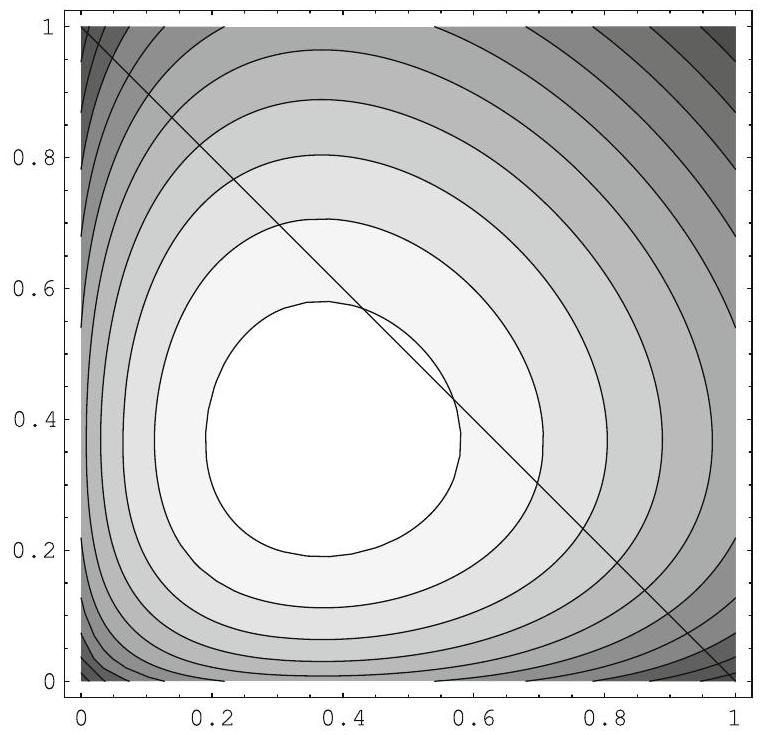
\includegraphics[max width=\textwidth, center]{2025_05_12_af19cd5e0d1b8a465ffeg-144}\\
and calculate

$$
p_{3}=p_{4}=\frac{1-\alpha}{2} .
$$

Now we can calculate the desired value

$$
P(B)=P(A, B)+P(\neg A, B)=p_{1}+p_{3}=\alpha \beta+\frac{1-\alpha}{2}=\alpha\left(\beta-\frac{1}{2}\right)+\frac{1}{2} .
$$

Substituting in $\alpha$ and $\beta$ yields

$$
P(B)=P(A)\left(P(B \mid A)-\frac{1}{2}\right)+\frac{1}{2}
$$

$P(B)$ is shown in Fig. 7.3 on page 140 for various values of $P(B \mid A)$. We see that in the two-value edge case, that is, when $P(B)$ and $P(B \mid A)$ take on the values 0 or 1, probabilistic inference returns the same value for $P(B)$ as the modus ponens. When $A$ and $B \mid A$ are both true, $B$ is also true. An interesting case is $P(A)=0$, in which $\neg A$ is true. Modus ponens cannot be applied here, but our formula results in the value $1 / 2$ for $P(B)$ irrespective of $P(B \mid A)$. When $A$ is false, we know nothing about $B$, which reflects our intuition exactly. The case where $P(A)=1$ and $P(B \mid A)=0$ is also covered by propositional logic. Here $A$ is true and $A \Rightarrow B$ false, and thus $A \wedge \neg B$ true. Then $B$ is false. The horizontal line in the figure means that we cannot make a prediction about $B$ in the case of $P(B \mid A)=1 / 2$. Between these points, $P(B)$ changes linearly for changes to $P(A)$ or $P(B \mid A)$.\\
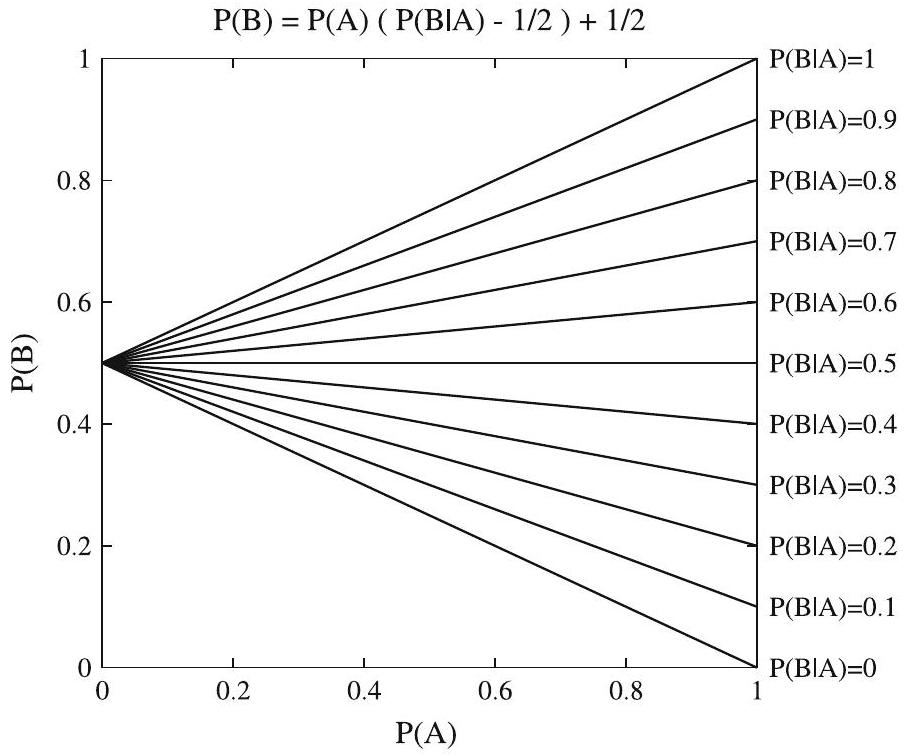
\includegraphics[max width=\textwidth, center]{2025_05_12_af19cd5e0d1b8a465ffeg-145}

Fig. 7.3 Curve array for $P(B)$ as a function of $P(A)$ for different values of $P(B \mid A)$

Theorem 7.3 Let there be a consistent ${ }^{5}$ set of linear probabilistic equations. Then there exists a unique maximum for the entropy function with the given equations as constraints. The MaxEnt distribution thereby defined has minimum information content under the constraints.

It follows from this theorem that there is no distribution which satisfies the constraints and has higher entropy than the MaxEnt distribution. A calculus that leads to lower entropy puts in additional ad hoc information, which is not justified.

Looking more closely at the above calculation of $P(B)$, we see that the two values $p_{3}$ and $p_{4}$ always occur symmetrically. This means that swapping the two variables does not change the result. Thus the end result is $p_{3}=p_{4}$. The so-called indifference of these two variables leads to them being set equal by MaxEnt. This relationship is valid generally:

Definition 7.5 If an arbitrary exchange of two or more variables in the Lagrange equations results in equivalent equations, these variables are called indifferent.

\footnotetext{${ }^{5}$ A set of probabilistic equations is called consistent if there is at least one solution, that is, one distribution which satisfies all equations.
}Theorem 7.4 If a set of variables $\left\{p_{i_{1}}, \ldots, p_{i_{k}}\right\}$ is indifferent, then the maximum of the entropy under the given constraints is at the point where $p_{i_{1}}=p_{i_{2}}=\cdots=p_{i_{k}}$.

With this knowledge we could have immediately set the two variables $p_{3}$ and $p_{4}$ equal (without solving the Lagrange equations).

\subsection*{7.2.2 Maximum Entropy Without Explicit Constraints}
We now look at the case in which no knowledge is given. This means that, other than the normalization condition

$$
p_{1}+p_{2}+\cdots+p_{n}=1,
$$

there are no constraints. All variables are therefore indifferent. Therefore we can set them equal and it follows that $p_{1}=p_{2}=\cdots=p_{n}=1 / n .^{6}$ For reasoning under uncertainty, this means that given a complete lack of knowledge, all worlds are equally probable. That is, the distribution is uniform. For example, in the case of two variables $A$ and $B$ it would be the case that

$$
P(A, B)=P(A, \neg B)=P(\neg A, B)=P(\neg A, \neg B)=1 / 4
$$

from which $P(A)=P(B)=1 / 2$ and $P(B \mid A)=1 / 2$ follow. The result for the two-dimensional case can be seen in Fig. 7.2 on page 139 because the marked condition is exactly the normalization condition. We see that the maximum of the entropy lies on the line at exactly $(1 / 2,1 / 2)$.

As soon as the value of a condition deviates from the one derived from the uniform distribution, the probabilities of the worlds shift. We show this in a further example. With the same descriptions as used above we assume that only

$$
P(B \mid A)=\beta
$$

is known. Thus $P(A, B)=P(B \mid A) P(A)=\beta P(A)$, from which $p_{1}=\beta\left(p_{1}+p_{2}\right)$ follows and we derive the two constraints

$$
\begin{gathered}
\beta p_{2}+(\beta-1) p_{1}=0 \\
p_{1}+p_{2}+p_{3}+p_{4}-1=0
\end{gathered}
$$

\footnotetext{${ }^{6}$ The reader may calculate this result by maximization of the entropy under the normalization condition (Exercise 7.5 on page 132).
}
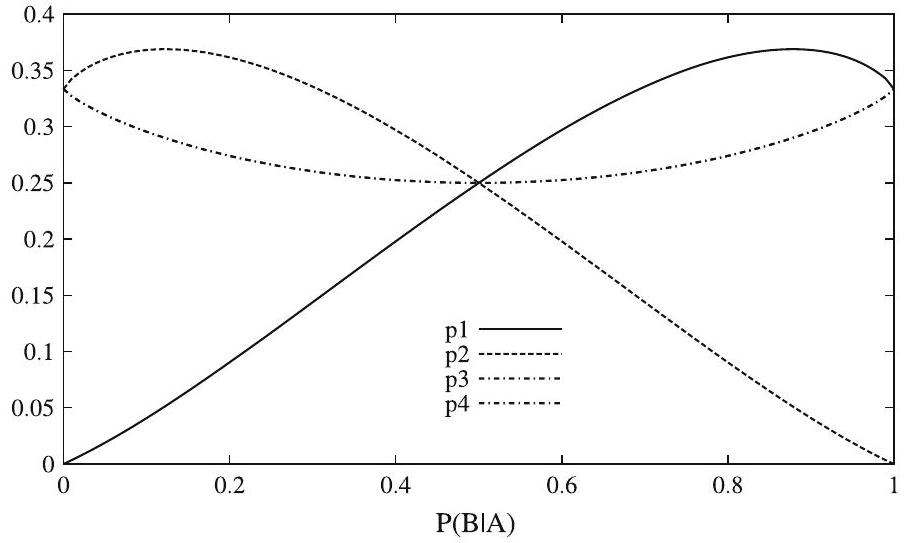
\includegraphics[max width=\textwidth, center]{2025_05_12_af19cd5e0d1b8a465ffeg-147}

Fig. $7.4 p_{1}, p_{2}, p_{3}, p_{4}$ in dependence on $\beta$

Here the Lagrange equations can no longer be solved symbolically so easily. A numeric solution of the Lagrange equations yields the picture represented in Fig. 7.4, which shows that $p_{3}=p_{4}$. We can already see this in the constraints, in which $p_{3}$ and $p_{4}$ are indifferent. For $P(B \mid A)=1 / 2$ we obtain the uniform distribution, which is no surprise. This means that the constraint for this value does not imply a restriction on the distribution. Furthermore, we can see that for small $P(B \mid A), P(A, B)$ is also small.

\subsection*{7.2.3 Conditional Probability Versus Material Implication}
We will now show that, for modeling reasoning, conditional probability is better than what is known in logic as material implication (to this end, also see [Ada75]). First we observe the truth table shown in Table 7.1, in which the conditional probability and material implication for the extreme cases of probabilities zero and one are compared. In both cases with false premises (which, intuitively, are critical cases), $P(B \mid A)$ is undefined, which makes sense.

Table 7.1 Truth table for material implication and conditional probability for propositional logic limit

\begin{center}
\begin{tabular}{|l|l|l|l|l|l|}
\hline
$A$ & $B$ & $A \Rightarrow B$ & $P(A)$ & $P(B)$ & $P(B \mid A)$ \\
\hline
$t$ & $t$ & $t$ & 1 & 1 & 1 \\
\hline
$t$ & $f$ & $f$ & 1 & 0 & 0 \\
\hline
$f$ & $t$ & $t$ & 0 & 1 & Undefined \\
\hline
$f$ & $f$ & $t$ & 0 & 0 & Undefined \\
\hline
\end{tabular}
\end{center}

Now we ask ourselves which value is taken on by $P(B \mid A)$ when arbitrary values $P(A)=\alpha$ and $P(B)=\gamma$ are given and no other information is known. Again we maximize entropy under the given constraints. As above we set

$$
p_{1}=P(A, B), \quad p_{2}=P(A, \neg B), \quad p_{3}=P(\neg A, B), \quad p_{4}=P(\neg A, \neg B)
$$

and obtain as constraints


\begin{gather*}
p_{1}+p_{2}=\alpha,  \tag{7.10}\\
p_{1}+p_{3}=\gamma,  \tag{7.11}\\
p_{1}+p_{2}+p_{3}+p_{4}=1 . \tag{7.12}
\end{gather*}


With this we calculate using entropy maximization (see Exercise 7.8 on page 173)

$$
p_{1}=\alpha \gamma, \quad p_{2}=\alpha(1-\gamma), \quad p_{3}=\gamma(1-\alpha), \quad p_{4}=(1-\alpha)(1-\gamma)
$$

From $p_{1}=\alpha \gamma$ it follows that $P(A, B)=P(A) \cdot P(B)$, which means that $A$ and $B$ are independent. Because there are no constraints connecting $A$ and $B$, the MaxEnt principle results in the independence of these variables. The right half of Table 7.1 on page 142 makes this easier to understand. From the definition

$$
P(B \mid A)=\frac{P(A, B)}{P(A)}
$$

it follows for the case $P(A) \neq 0$, that is, when the premise is not false, because $A$ and $B$ are independent, that $P(B \mid A)=P(B)$. For the case $P(A)=0, P(B \mid A)$ remains undefined.

\subsection*{7.2.4 MaxEnt-Systems}
As previously mentioned, due to the nonlinearity of the entropy function, MaxEnt optimization usually cannot be carried out symbolically for non-trivial problems. Thus two systems were developed for numerical entropy maximization. The first system, SPIRIT (Symmetrical Probabilistic Intensional Reasoning in Inference Networks in Transition, \href{http://www.xspirit.de}{www.xspirit.de}), [RM96] was built at Fernuniversität Hagen. The second, PIT (Probability Induction Tool) was developed at the Munich Technical University [Sch96, ES99, SE00]. We will now briefly introduce PIT.

The PIT system uses the sequential quadratic programming (SQP) method to find an extremum of the entropy function under the given constraints. As input, PIT\\
expects data containing the constraints. For example, the constraints $P(A)=\alpha$ and $P(B \mid A)=\beta$ from Sect. 7.2.1 have the form

\begin{verbatim}
var A{t,f}, B{t,f};
P([A=t]) = 0.6;
P([B=t] | [A=t]) = 0.3;
QP([B=t]);
QP([B=t] | [A=t]);
\end{verbatim}

Because PIT performs a numerical calculation, we have to input explicit probability values. The second to last row contains the query QP ([B=t]). This means that $P(B)$ is the desired value. At \href{http://www.pit-systems.de}{www.pit-systems.de} under "Examples" we now put this input into a blank input page ("Blank Page") and start PIT. As a result we get

\begin{center}
\begin{tabular}{llll}
\hline
Nr. & Truth value & Probability & Query \\
\hline
1 & UNSPECIFIED & $3.800 \mathrm{e}-01$ & QP $([B=t]) ;$ \\
\hline
2 & UNSPECIFIED & $3.000 \mathrm{e}-01$ & QP $([A=t]-\mid>[B=t]) ;$ \\
\hline
\end{tabular}
\end{center}

and from there read off $P(B)=0.38$ and $P(B \mid A)=0.3$.

\subsection*{7.2.5 The Tweety Example}
We now show, using the Tweety example from Sect. 4.3, that probabilistic reasoning and in particular MaxEnt are non-monotonic and model everyday reasoning very well. We model the relevant rules with probabilities as follows:

$$
\begin{array}{lll}
P(\text { bird } \mid \text { penguin }) & =1 & \\
P(\text { flies } \mid \text { bird }) & \in[0.95,1] & \text { "penguins are birds" } \\
P(\text { flies } \mid \text { penguin }) & =0 & \text { "(almost all) birds can fly" } \\
& \text { "penguins cannot fly" }
\end{array}
$$

The first and third rules represent firm predictions, which can also be easily formulated in logic. In the second, however, we express our knowledge that almost all birds can fly by means of a probability interval. With the PIT input data

\begin{verbatim}
var penguin{yes,no}, bird{yes,no}, flies{yes,no};
P([bird=yes] | [penguin=yes]) = 1;
P([flies=yes] | [bird=yes]) IN [0.95,1];
P([flies=yes] | [penguin=yes]) = 0;
QP([flies=yes]| [penguin=yes]);
\end{verbatim}

we get back the correct answer

\begin{center}
\begin{tabular}{llll}
\hline
Nr. & Truthvalue & Probability & Query \\
\hline
1 & UNSPECIFIED & $0.000 \mathrm{e}+00$ & QP $([$ penguin $=$ yes $]-\mid>[$ flies $=$ yes $]) ;$ \\
\hline
\end{tabular}
\end{center}

with the proposition that penguins cannot fly. ${ }^{7}$ The explanation for this is very simple. With $P($ flies $\mid$ bird $) \in[0.95,1]$ it is possible that there are non-flying birds. If this rule were replaced by $P($ flies $\mid$ bird $)=1$, then PIT would not be able to do anything and would output an error message about inconsistent constraints.

In this example we can easily see that probability intervals are often very helpful for modeling our ignorance about exact probability values. We could have made an even fuzzier formulation of the second rule in the spirit of "normally birds fly" with $P($ flies $\mid$ bird $) \in(0.5,1]$. The use of the half-open interval excludes the value 0.5 .

It has already been shown in [Pea88] that this example can be solved using probabilistic logic, even without MaxEnt. In [Sch96] it is shown for a number of demanding benchmarks for non-monotonic reasoning that these can be solved elegantly with MaxEnt. In the following section we introduce a successful practical application of MaxEnt in the form of a medical expert system.

\subsection*{7.3 Lexmed, an Expert System for Diagnosing Appendicitis}
The medical expert system Lexmed, which uses the MaxEnt method, was developed at the Ravensburg-Weingarten University of Applied Sciences by Manfred Schramm, Walter Rampf, and the author, in cooperation with the Weingarten 14-Nothelfer Hospital [SE00, Le999]. ${ }^{8}$ The acronym Lexmed stands for learning expert system for medical diagnosis.

\subsection*{7.3.1 Appendicitis Diagnosis with Formal Methods}
The most common serious cause of acute abdominal pain [dD91] is appendicitisan inflammation of the appendix, a blind-ended tube connected to the cecum. Even today, diagnosis can be difficult in many cases [ $\mathrm{OFY}^{+} 95$ ]. For example, up to about $20 \%$ of the removed appendices are without pathological findings, which means that the operations were unnecessary. Likewise, there are regularly cases in which an inflamed appendix is not recognized as such.

Since as early as the beginning of the 1970s, there have been attempts to automate the diagnosis of appendicitis, with the goal of reducing the rate of false\\
${ }^{7}$ QP ([penguin=yes]-|> [flies=yes]) is an alternative form of the PIT syntax for QP ([flies=yes] | [penguin=yes]).\\
${ }^{8}$ The project was financed by the German state of Baden-Württemberg, the health insurance company AOK Baden-Württemberg, the Ravensburg-Weingarten University of Applied Sciences, and the 14 Nothelfer Hospital in Weingarten.\\[0pt]
diagnoses [dDLS+72, OPB94, OFY+95]. Especially noteworthy is the expert system for diagnosis of acute abdominal pain, developed by de Dombal in Great Britain. It was made public in 1972, thus distinctly earlier than the famous system MYCIN.

Nearly all of the formal diagnostic processes used in medicine to date have been based on scores. Score systems are extremely easy to apply: For each value of a symptom (for example fever or lower right stomach pain) the doctor notes a certain number of points. If the sum of the points is over a certain value (threshold), a certain decision is recommended (for example operation). For $n$ symptoms $S_{1}, \ldots, S_{n}$ a score for appendicitis can be described formally as

$$
\text { Diagnose }= \begin{cases}\text { Appendicitis } & \text { if } w_{1} S_{1}+\cdots+w_{n} S_{n}>\Theta, \\ \text { negative } & \text { else. }\end{cases}
$$

With scores, a linear combination of symptom values is thus compared with a threshold $\Theta$. The weights of the symptoms are extracted from databases using statistical methods. The advantage of scores is their simplicity of application. The weighted sum of the points can be computed by hand easily and a computer is not needed for the diagnosis.

Because of the linearity of this method, scores are too weak to model complex relationships. Since the contribution $w_{i} S_{i}$ of a symptom $S_{i}$ to the score is calculated independently of the other symptoms, it is clear that score systems cannot take any "context" into account. Principally, they cannot distinguish between combinations of symptoms, for example they cannot distinguish between the white blood cell count of an old patient and that of a young patient.

For a fixed given set of symptoms, conditional probability is much more powerful than scores for making predictions because the latter cannot describe the dependencies between different symptoms. We can show that scores implicitly assume that all symptoms are independent.

When using scores, yet another problem comes up. To arrive at a good diagnosis quality, we must put strict requirements on the databases used to statistically determine the weights $w_{i}$. In particular they must be representative of the set of patients in the area in which the diagnosis system is used. This is often difficult, if not impossible, to guarantee. In such cases, scores and other statistical methods either cannot be used, or will have a high rate of errors.

\subsection*{7.3.2 Hybrid Probabilistic Knowledge Base}
Complex probabilistic relationships appear frequently in medicine. With Lexmed, these relationships can be modeled well and calculated quickly. Here the use of probabilistic propositions, with which uncertain and incomplete information can be expressed and processed in an intuitive and mathematically grounded way, is essential. The following question may serve as a typical query against the expert system: "How high is the probability of an inflamed appendix if the patient is a 23-year-old man with pain in the right lower abdomen and a white blood cell count

Table 7.2 Symptoms used for the query in Lexmed and their values. The number of values for the each symptom is given in the column marked \#

\begin{center}
\begin{tabular}{|l|l|l|l|}
\hline
Symptom & Values & \# & Short \\
\hline
Gender & Male, female & 2 & Sex2 \\
\hline
Age & 0-5, 6-10, 11-15, 16-20, 21-25, 26-35, 36-45, 46-55, 56-65, 65- & 10 & Age10 \\
\hline
Pain 1st Quad. & Yes, no & 2 & P1Q2 \\
\hline
Pain 2nd Quad. & Yes, no & 2 & P2Q2 \\
\hline
Pain 3rd Quad. & Yes, no & 2 & P3Q2 \\
\hline
Pain 4th Quad. & Yes, no & 2 & P4Q2 \\
\hline
Guarding & Local, global, none & 3 & Gua3 \\
\hline
Rebound tenderness & Yes, no & 2 & Reb2 \\
\hline
Pain on tapping & Yes, no & 2 & Tapp2 \\
\hline
Rectal pain & Yes, no & 2 & RecP2 \\
\hline
Bowel sounds & Weak, normal, increased, none & 4 & BowS4 \\
\hline
Abnormal ultrasound & Yes, no & 2 & Sono2 \\
\hline
Abnormal urine sedim. & Yes, no & 2 & Urin2 \\
\hline
Temperature (rectal) & -37.3, 37.4-37.6, 37.7-38.0, 38.1-38.4, 38.5-38.9, 39.0- & 6 & TRec6 \\
\hline
Leukocytes & 0-6k, 6k-8k, 8k-10k, 10k-12k, 12k-15k, 15k-20k, 20k- & 7 & Leuko7 \\
\hline
Diagnosis & Inflamed, perforated, negative, other & 4 & Diag4 \\
\hline
\end{tabular}
\end{center}

of 13,000 ?" Formulated as conditional probability, using the names and value ranges for the symptoms used in Table 7.2, this reads

$$
\begin{aligned}
& P(\text { Diag } 4=\text { inflamed } \vee \text { Diag } 4=\text { perforated } \mid \\
& \quad \text { Sex } 2=\text { male } \wedge \text { Age } 10 \in 21-25 \wedge \text { Leuko } 7 \in 12 k-15 k) .
\end{aligned}
$$

By using probabilistic propositions, Lexmed has the ability to use information from non-representative databases because this information can be complemented appropriately from other sources. Underlying Lexmed is a database which only contains data about patients whose appendixes were surgically removed. With statistical methods, (about 400) rules are generated which compile the knowledge contained in the database into an abstracted form [ES99]. Because there are no patients in this database who were suspected of having appendicitis but had negative diagnoses (that is, not requiring treatment), ${ }^{9}$ there is no knowledge about negative patients in the database. Thus knowledge from other sources must be added in. In Lexmed therefore the rules gathered from the database are complemented by (about 100) rules from medical experts and the medical literature. This results in a hybrid probabilistic database, which contains knowledge extracted from data as well as knowledge explicitly formulated by experts. Because both types of rules are formulated as conditional probabilities (see for example (7.14) on page 152), they can be easily combined, as shown in Fig. 7.5 on page 148 and with more details in Fig. 7.7 on page 150.

\footnotetext{${ }^{9}$ These negative diagnoses are denoted "non-specific abdominal pain" (NSAP).
}
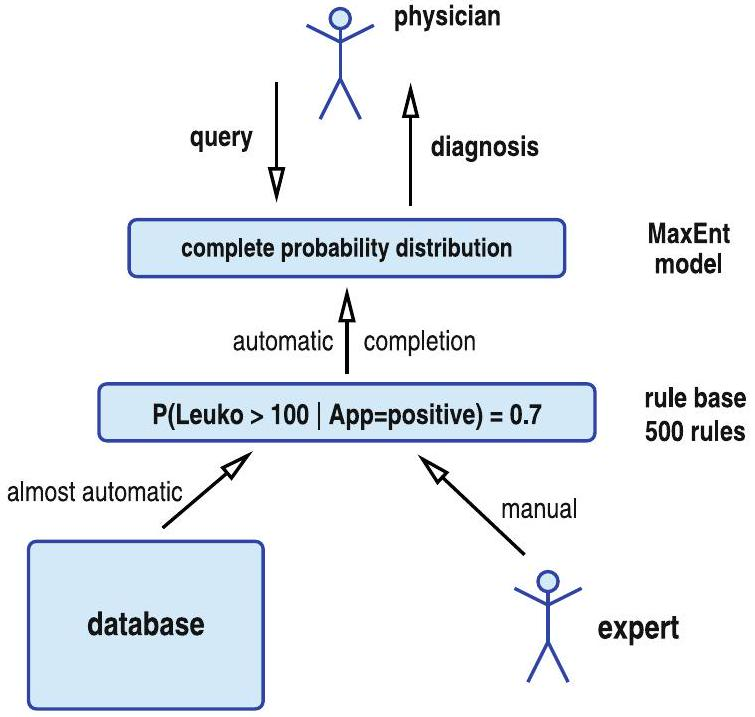
\includegraphics[max width=\textwidth, center]{2025_05_12_af19cd5e0d1b8a465ffeg-153}

Fig. 7.5 Probabilistic rules are generated from data and expert knowledge, which are integrated in a rule base (knowledge base) and finally made complete using the MaxEnt method

Lexmed calculates the probabilities of various diagnoses using the probability distribution of all relevant variables (see Table 7.2 on page 147). Because all 14 symptoms used in Lexmed and the diagnoses are modeled as discrete variables (even continuous variables like the leukocyte value are divided into ranges), the size of the distribution (that is, the size of the event space) can be determined using Table 7.2 on page 147 as the product of the number of values of all symptoms, or

$$
2^{10} \cdot 10 \cdot 3 \cdot 4 \cdot 6 \cdot 7 \cdot 4=20643840
$$

elements. Due to the normalization condition from Theorem 7.1 on page 129, it thus has 20643839 independent values. Every rule set with fewer than 20643839 probability values potentially does not completely describe this event space. To be able to answer any arbitrary query, the expert system needs a complete distribution. The construction of such an extensive, consistent distribution using statistical methods is very difficult. ${ }^{10}$ To require from a human expert all 20643839 values for the distribution (instead of the aforementioned 100 rules) would essentially be impossible.

Here the MaxEnt method comes into play. The generalization of about 500 rules to a complete probability model is done in Lexmed by maximizing the entropy with the 500 rules as constraints. An efficient encoding of the resulting MaxEnt distribution leads to response times for the diagnosis of around one second.

\footnotetext{${ }^{10}$ The task of generating a function from a set of data is known as machine learning. We will cover this thoroughly in Chap. 8.
}\begin{center}
\begin{tabular}{|l|l|l|l|}
\hline
Personal Details & unknown & values &  \\
\hline
Gender & $-$ & $\checkmark$ male $\sim$ female & ? \\
\hline
Age-group & r & ( $0.5 \sim 6-10 \sim 11-15 \sim 16-20 \cdot 21-25 \sim 26-35 \sim 36-45 \sim$ $46-55 \sim 56-65 \sim 65-$ & 
\includegraphics[max width=\textwidth]{2025_05_12_af19cd5e0d1b8a465ffeg-154}
 \\
\hline
Results of examination & not done & values &  \\
\hline
1st quadrant & - & $\checkmark$ yes $\sim$ no & ? \\
\hline
2nd quadrant & - & ( yes ) no & ? \\
\hline
3rd quadrant & c & - yes \~{} no & ? \\
\hline
4th quadrant & 0 & $\checkmark$ yes $\sim$ no & ? \\
\hline
guarding & c & - local $\Gamma$ global $C$ none & ? \\
\hline
rebound tenderness & r & - yes $\sim$ no & ? \\
\hline
pain on tapping & c & - yes $\sim$ no & ? \\
\hline
rectal pain & - & $r$ yes $r$ no & ? \\
\hline
bowel sounds & c & $\checkmark$ weak $*$ normal $\sim$ increased $\sim$ none & ? \\
\hline
abnormal ultrasound & - & $\checkmark$ yes $\sim$ no & ? \\
\hline
abnormal urine sediment & - & $\checkmark$ yes $\sim$ no & ? \\
\hline
temperature range (rectal) & r & $(37.3) 37.437 .6) 37.738 .0 \sim 38.138 .4 \cdot 38.538 .9 \sim 39.0$ & ? \\
\hline
leucocyte count & c & $\sim 0-6 \mathrm{k} \sim 6 \mathrm{k}-8 \mathrm{k} \sim 8 \mathrm{k}-10 \mathrm{k} \sim 10 \mathrm{k}-12 \mathrm{k} \sim 12 \mathrm{k}-15 \mathrm{k} \sim 15 \mathrm{k}-20 \mathrm{k} \sim 20 \mathrm{k}-$ & ? \\
\hline
 &  &  &  \\
\hline
\multicolumn{4}{|c|}{Result of the PIT diagnosis} \\
\hline
Diagnosis & App. inflamed & App. perforated & Other \\
\hline
Probability & 0.70 & 0.17 & 0.07 \\
\hline
\end{tabular}
\end{center}

Fig. 7.6 The Lexmed input mask for input of the examined symptoms and below it the output of the resulting diagnosis probabilities

\subsection*{7.3.3 Application of Lexmed}
The usage of Lexmed is simple and self-explanatory. The doctor visits the Lexmed home page at \href{http://www.lexmed.de}{www.lexmed.de}. ${ }^{11}$ For an automatic diagnosis, the doctor inputs the results of his examination into the input form in Fig. 7.6. After one or two seconds he receives the probabilities for the four different diagnoses as well as a suggestion for a treatment (Sect. 7.3.5). If certain examination results are missing as input (for example the sonogram results), then the doctor chooses the entry not examined. Naturally the certainty of the diagnosis is higher when more symptom values are input.

\footnotetext{${ }^{11}$ A version with limited functionality is accessible without a password.
}
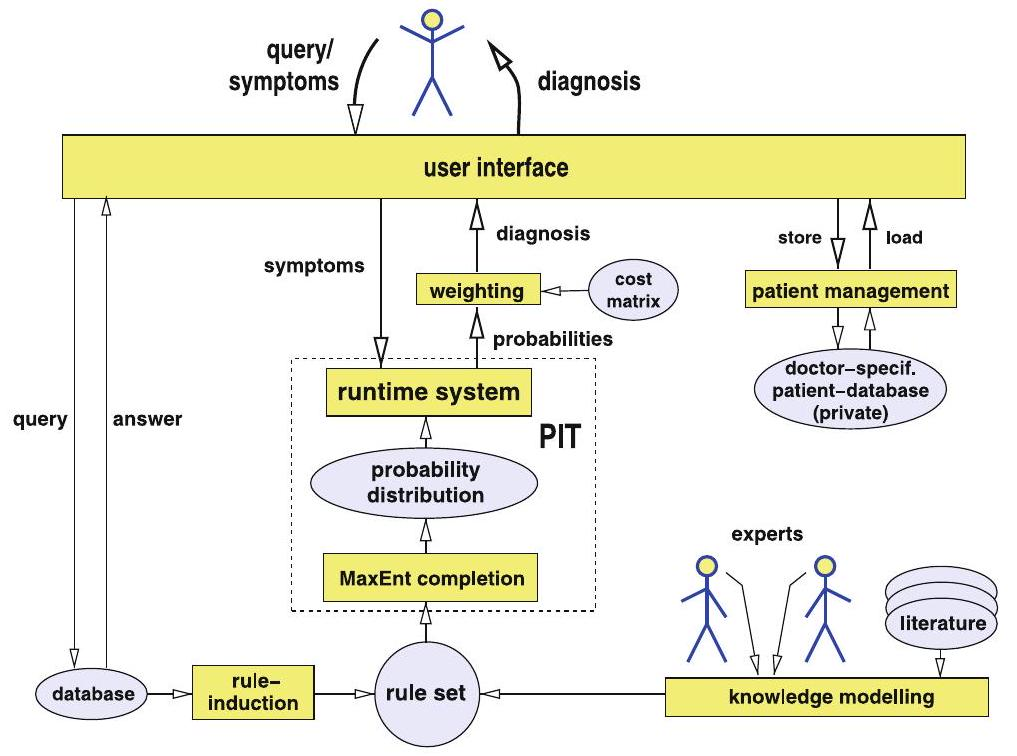
\includegraphics[max width=\textwidth, center]{2025_05_12_af19cd5e0d1b8a465ffeg-155}

Fig. 7.7 Rules are generated from the database as well as from expert knowledge. From these, MaxEnt creates a complete probability distribution. For a user query, the probability of every possible diagnosis is calculated. Using the cost matrix (see Sect. 7.3.5) a decision is then suggested

Each registered user has access to a private patient database, in which input data can be archived. Thus data and diagnoses from earlier patients can be easily compared with those of a new patient. An overview of the processes in Lexmed is given in Fig. 7.7.

\subsection*{7.3.4 Function of Lexmed}
Knowledge is formalized using probabilistic propositions. For example, the proposition

$$
P(\text { Leuko } 7>20000 \mid \text { Diag } 4=\text { inflamed })=0.09
$$

gives a frequency of $9 \%$ for a leukocyte value of more than 20,000 in case of an inflamed appendix. ${ }^{12}$

\section*{Learning of Rules by Statistical Induction}
The raw data in Lexmed's database contain 54 different (anonymized) values for 14,646 patients. As previously mentioned, only patients whose appendixes were surgically removed are included in this database. Of the 54 attributes used in the

\footnotetext{${ }^{12}$ Instead of individual numerical values, intervals can also be used here (for example [0.06, 0.12]).
}
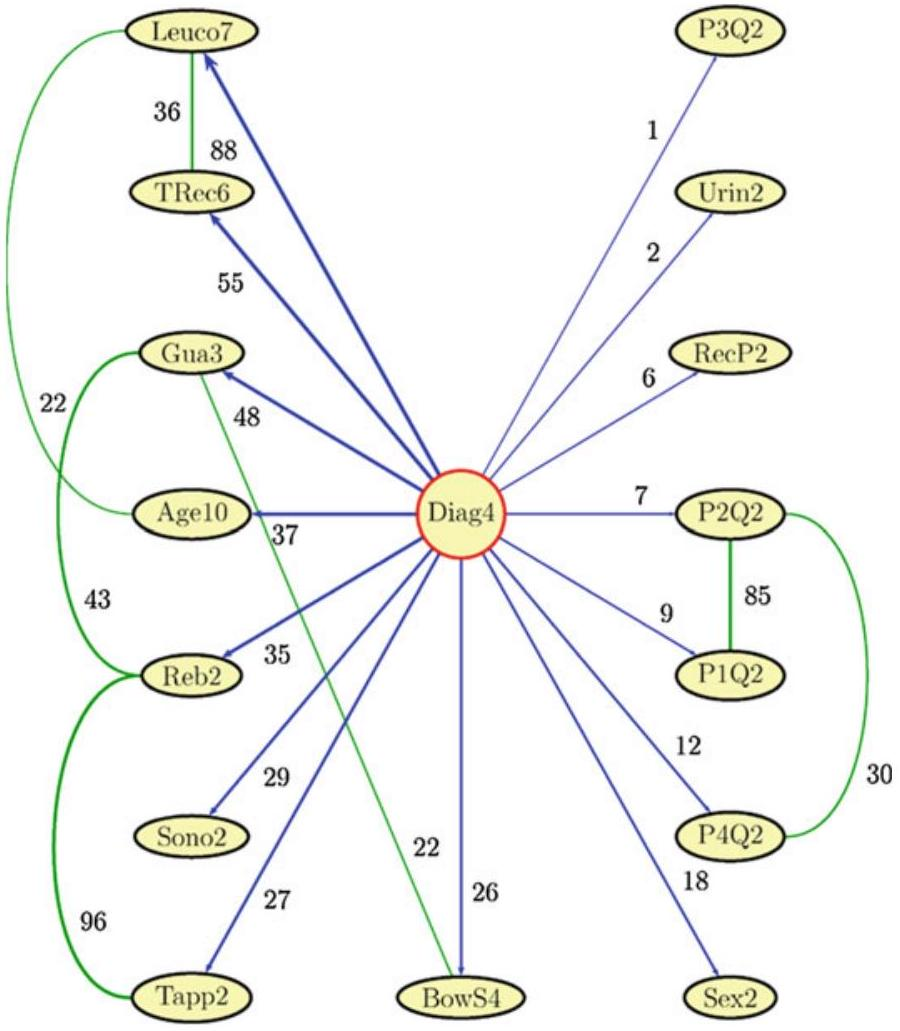
\includegraphics[max width=\textwidth, center]{2025_05_12_af19cd5e0d1b8a465ffeg-156}

Fig. 7.8 Dependency graph computed from the database\\
database, after a statistical analysis the 14 symptoms shown in Table 7.2 on page 147 were used. Now the rules are created from this database in two steps. The first step determines the dependency structure of the symptoms. The second step fills this structure with the respective probability rules. ${ }^{13}$

Determining the Dependency Graph The graph in Fig. 7.8 contains for each variable (the symptom and the diagnosis) a node and directed edges which connect various nodes. The thickness of the edges between the variables represents a measure of the statistical dependency or correlation of the variables. The correlation of two independent variables is equal to zero. The pair correlation for each of the 14 symptoms with Diag4 was computed and listed in the graph. Furthermore, all triple correlations between the diagnosis and two symptoms were calculated. Of these, only the strongest values have been drawn as additional edges between the two participating symptoms.

\footnotetext{${ }^{13}$ For a systematic introduction to machine learning we refer the reader to Chap. 8.
}\begin{verbatim}
P([Leuco7=0-6k] | [Diag4=negativ] * [Age10=16-20]) = [0.132,0.156];
P([Leuco7=6-8k] | [Diag4=negativ] * [Age10=16-20]) = [0.257,0.281];
P([Leuco7=8-10k] | [Diag4=negativ] * [Age10=16-20]) = [0.250,0.274];
P([Leuco7=10-12k] | [Diag4=negativ] * [Age10=16-20]) = [0.159,0.183];
P([Leuco7=12-15k] [Diag4=negativ] * [Age10=16-20]) = [0.087,0.112];
P([Leuco7=15-20k] | [Diag4=negativ] * [Age10=16-20]) = [0.032,0.056];
P([Leuco7=20k-] | [Diag4=negativ] * [Age10=16-20]) = [0.000,0.023];
P([Leuco7=0-6k] | [Diag4=negativ] * [Age10=21-25]) = [0.132,0.172];
P([Leuco7=6-8k] | [Diag4=negativ] * [Age10=21-25]) = [0.227,0.266];
P([Leuco7=8-10k] | [Diag4=negativ] * [Age10=21-25]) = [0.211,0.250];
P([Leuco7=10-12k] | [Diag4=negativ] * [Age10=21-25]) = [0.166,0.205];
P([Leuco7=12-15k] | [Diag4=negativ] * [Age10=21-25]) = [0.081,0.120];
P([Leuco7=15-20k] | [Diag4=negativ] * [Age10=21-25]) = [0.041,0.081];
P([Leuco7=20k-] | [Diag4=negativ] * [Age10=21-25]) = [0.004,0.043];
\end{verbatim}

Fig. 7.9 Some of the Lexmed rules with probability intervals. "*" stands for " $\wedge$ " here

Estimating the Rule Probabilities The structure of the dependency graph describes the structure of the learned rules. ${ }^{14}$ The rules here have different complexities: there are rules which only describe the distribution of the possible diagnoses (a priori rules, for example (7.13)), rules which describe the dependency between the diagnosis and a symptom (rules with simple conditions, for example (7.14)), and finally rules which describe the dependency between the diagnosis and two symptoms, as given in Fig. 7.9 in Pit syntax.

\[
\begin{array}{r}
P(\text { Diag } 4=\text { inflamed })=0.40, \\
P(\text { Sono } 2=\text { yes } \mid \text { Diag } 4=\text { inflamed })=0.43, \\
P(P 4 Q 2=\text { yes } \mid \text { Diag } 4=\text { inflamed } \wedge P 2 Q 2=\text { yes })=0.61 . \tag{7.15}
\end{array}
\]

To keep the context dependency of the saved knowledge as small as possible, all rules contain the diagnosis in their conditions and not as conclusions. This is quite similar to the construction of many medical books with formulations of the kind "With appendicitis we usually see ...". As previously shown in Example 7.6 on page 133, however, this does not present a problem because, using the Bayesian formula, Lexmed automatically puts these rules into the right form.

The numerical values for these rules are estimated by counting their frequency in the database. For example, the value in (7.14) is given by counting and calculating

$$
\frac{\mid \text { Diag4 }=\text { inflamed } \wedge \text { Sono } 2=\text { yes } \mid}{\mid \text { Diag } 4=\text { inflamed } \mid}=0.43 .
$$

\footnotetext{${ }^{14}$ The difference between this and a Bayesian network is, for example, that the rules are equipped with probability intervals and that only after applying the principle of maximum entropy is a unique probability model produced.
}\section*{Expert Rules}
Because the appendicitis database only contains patients who have undergone the operation, rules for non-specific abdominal pain (NSAP) receive their values from propositions of medical experts. The experiences in Lexmed confirm that the probabilistic rules are easy to read and can be directly translated into natural language. Statements by medical experts about frequency relationships of specific symptoms and the diagnosis, whether from the literature or as the result of an interview, can therefore be incorporated into the rule base with little expense. To model the uncertainty of expert knowledge, the use of probability intervals has proven effective. The expert knowledge was primarily acquired from the participating surgeons, Dr. Rampf and Dr. Hontschik, and their publications [Hon94].

Once the expert rules have been created, the rule base is finished. Then the complete probability model is calculated with the method of maximum entropy by the Pit-system.

\section*{Diagnosis Queries}
Using its efficiently stored probability model, Lexmed calculates the probabilities for the four possible diagnoses within a few seconds. For example, we assume the following output:

\begin{center}
\begin{tabular}{lllll}
\hline
 & \multicolumn{4}{l}{Results of the PIT diagnosis} \\
\cline { 2 - 5 }
Diagnosis & Appendix inflamed & Appendix perforated & Negative & Other \\
\hline
Probability & 0.24 & 0.16 & 0.57 & 0.03 \\
\hline
\end{tabular}
\end{center}

A decision must be made based on these four probability values to pursue one of the four treatments: operation, emergency operation, stationary observation, or ambulant observation. ${ }^{15}$ While the probability for a negative diagnosis in this case outweighs the others, sending the patient home as healthy is not a good decision. We can clearly see that, even when the probabilities of the diagnoses have been calculated, the diagnosis is not yet finished.

Rather, the task is now to derive an optimal decision from these probabilities. To this end, the user can have Lexmed calculate a recommended decision.

\subsection*{7.3.5 Risk Management Using the Cost Matrix}
How can the computed probabilities now be translated optimally into decisions? A naive algorithm would assign a decision to each diagnosis and ultimately select the decision that corresponds to the highest probability. Assume that the computed probabilities are 0.40 for the diagnosis appendicitis (inflamed or perforated), 0.55 for the diagnosis negative, and 0.05 for the diagnosis other. A naive algorithm would now choose the (too risky) decision "no operation" because it corresponds to the diagnosis with the higher probability. A better method consists of comparing

\footnotetext{${ }^{15}$ Ambulant observation means that the patient is released to stay at home.
}Table 7.3 The cost matrix of LeXMED together with a patient's computed diagnosis probabilities

\begin{center}
\begin{tabular}{|l|l|l|l|l|l|}
\hline
\multirow[t]{3}{*}{Therapy} & \multicolumn{4}{|l|}{Probability of various diagnoses} & \multirow{3}{*}{} \\
\hline
 & Inflamed & Perforated & Negative & Other &  \\
\hline
 & 0.25 & 0.15 & 0.55 & 0.05 &  \\
\hline
Operation & 0 & 500 & 5800 & 6000 & 3565 \\
\hline
Emergency operation & 500 & 0 & 6300 & 6500 & 3915 \\
\hline
Ambulant observ. & 12000 & 150000 & 0 & 16500 & 26325 \\
\hline
Other & 3000 & 5000 & 1300 & 0 & 2215 \\
\hline
Stationary observ. & 3500 & 7000 & 400 & 600 & 2175 \\
\hline
\end{tabular}
\end{center}

the costs of the possible errors that can occur for each decision. The error is quantified in the form of "(hypothetical) additional cost of the current decision compared to the optimum". The given values contain the costs to the hospital, to the insurance company, the patient (for example risk of post-operative complications), and to other parties (for example absence from work), taking into account long term consequences. These costs are given in Table 7.3.

The entries are finally averaged for each decision, that is, summed while taking into account their frequencies. These are listed in the last column in Table 7.3. Finally, the decision with the smallest average cost of error is suggested. In Table 7.3 the matrix is given together with the probability vector calculated for a patient (in this case: $(0.25,0.15,0.55,0.05)$ ). The last column of the table contains the result of the calculations of the average expected costs of the errors. The value of Operation in the first row is thus calculated as $0.25 \cdot 0+0.15 \cdot 500+0.55 \cdot 5800+$ $0.05 \cdot 6000=3565$, a weighted average of all costs. The optimal decisions are entered with (additional) costs of 0 . The system decides on the treatment with the minimal average cost. It thus is an example of a cost-oriented agent.

\section*{Cost Matrix in the Binary Case}
To better understand the cost matrix and risk management we will now restrict the Lexmed system to the two-value decision between the diagnosis appendicitis with probability

$$
p_{1}=P(\text { appendicitis })=P(\text { Diag } 4=\text { inflamed })+P(\text { Diag } 4=\text { perforated })
$$

and NSAP with the probability

$$
p_{2}=P(N S A P)=P(\text { Diag } 4=\text { negative })+P(\text { Diag } 4=\text { other })
$$

The only available treatments are operation and ambulant observation.\\
The cost matrix is thus a $2 \times 2$ matrix of the form

$$
\left(\begin{array}{cc}
0 & k_{2} \\
k_{1} & 0
\end{array}\right)
$$

The two zeroes in the diagonal stand for the correct decision operation in the case of appendicitis and ambulant observation for NSAP. The parameter $k_{2}$ stands for the expected costs which occur when a patient without an inflamed appendix is operated on. This error is called a false positive. On the other hand, the decision ambulant observation in the case of appendicitis is a false negative. The probability vector $\left(p_{1}, p_{2}\right)^{T}$ is now multiplied by this matrix and we obtain the vector

$$
\left(k_{2} p_{2}, k_{1} p_{1}\right)^{T}
$$

with the average additional cost for the two possible treatments. Because the decision only takes into account the relationship of the two components, the vector can be multiplied by any scalar factor. We choose $1 / k_{1}$ and obtain $\left(\left(k_{2} / k_{1}\right) p_{2}, p_{1}\right)$. Thus only the relationship $k=k_{2} / k_{1}$ is relevant here. The same result is obtained by the simpler cost matrix

$$
\left(\begin{array}{ll}
0 & k \\
1 & 0
\end{array}\right)
$$

which only contains the variable $k$. This parameter is very important because it determines risk management. By changing $k$ we can fit the "working point" of the diagnosis system. For $k \rightarrow \infty$ the system is put in an extremely risky setting because no patient will ever be operated on, with the consequence that it gives no false positive classifications, but many False negatives. In the case of $k=0$ the conditions are in exact reverse and all patients are operated upon.

\subsection*{7.3.6 Performance}
Lexmed is intended for use in a medical practice or ambulance. Prerequisites for the use of Lexmed are acute abdominal pain for several hours (but less than five days). Furthermore, Lexmed is (currently) specialized for appendicitis, which means that for other illnesses the system contains very little information.

In the scope of a prospective study, a representative database with 185 cases was created in the 14 Nothelfer Hospital. It contains the hospital's patients who came to the clinic after several hours of acute abdominal pain and suspected appendicitis. From these patients, the symptoms and the diagnosis (verified from a tissue sample in the case of an operation) is noted.

If the patients were released to go home (without operation) after a stay of several hours or 1-2 days with little or no complaint, it was afterwards inquired by telephone whether the patient remained free of symptoms or whether a positive diagnosis was found in subsequent treatment.

To simplify the representation and make for a better comparison to similar studies, Lexmed was restricted to the two-value distinction between appendicitis and NSAP, as described in Sect. 7.3.5. Now $k$ is varied between zero and infinity\\
and for every value of $k$ the sensitivity and specificity are measured against the test data. Sensitivity measures


\begin{equation*}
P(\text { classified positive } \mid \text { positive })=\frac{\mid \text { positive and classified positive } \mid}{\mid \text { positive } \mid}, \tag{7.16}
\end{equation*}


that is, the relative portion of positive cases which are correctly identified. It indicates how sensitive the diagnostic system is. Specificity, on the other hand, measures


\begin{equation*}
P(\text { classified negative } \mid \text { negative })=\frac{\mid \text { negative and classified negative } \mid}{\mid \text { negative } \mid}, \tag{7.17}
\end{equation*}


that is, the relative portion of negative cases which are correctly identified.\\
We give the results of the sensitivity and specificity in Fig. 7.10 for $0 \leq k<\infty$. This curve is denoted the ROC curve, or receiver operating characteristic. Before we come to the analysis of the quality of Lexmed, a few words about the meaning of the ROC curve. The line bisecting the diagram diagonally is drawn in for orientation. All points on this line correspond to a random decision. For example, the point (0.2, 0.2) corresponds to a specificity of 0.8 with a sensitivity of 0.2 . We can arrive at this quite easily by classifying a new case, without looking at it, with probabilities 0.2 for positive and 0.8 for negative. Every knowledge-based diagnosis system must therefore generate a ROC which clearly lies above the diagonal.\\
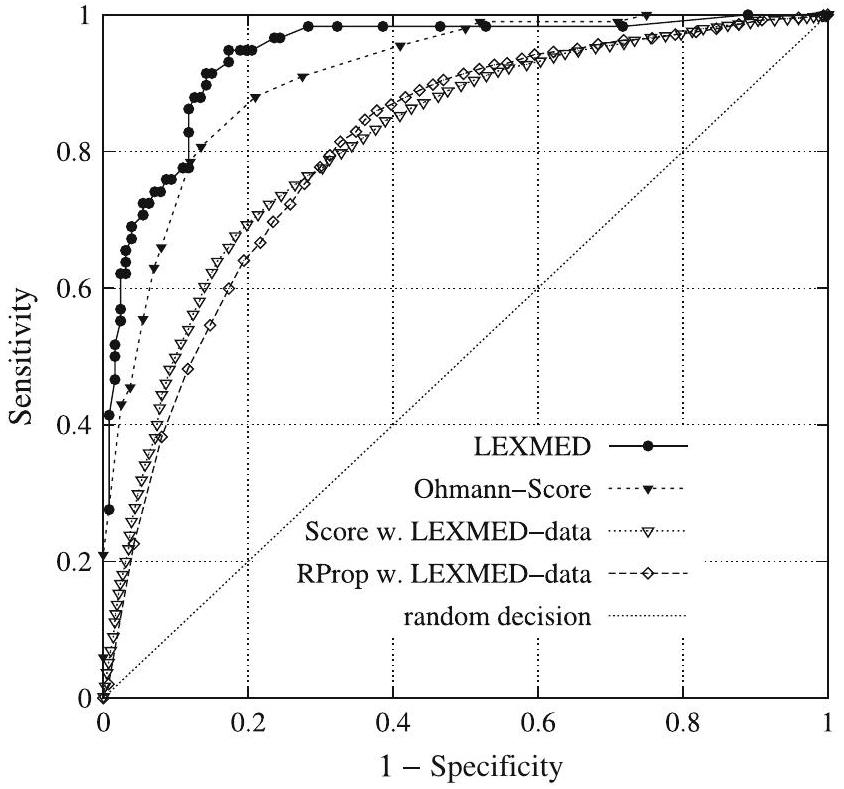
\includegraphics[max width=\textwidth, center]{2025_05_12_af19cd5e0d1b8a465ffeg-161}

Fig. 7.10 ROC curve from Lexmed compared with the Ohmann score and two additional models

The extreme values in the ROC curve are also interesting. At point $(0,0)$ all three curves intersect. The corresponding diagnosis system would classify all cases as negative. The other extreme value $(1,1)$ corresponds to a system which would decide to do the operation for every patient and thus has a sensitivity of 1 . We could call the ROC curve the characteristic curve for two-value diagnostic systems. The ideal diagnostic system would have a characteristic curve which consists only of the point $(0,1)$, and thus has $100 \%$ specificity and $100 \%$ sensitivity.

Now let us analyse the ROC curve. At a sensitivity of $88 \%$, Lexmed attains a specificity of $87 \%(k=0.6)$. For comparison, the Ohmann score, an established, well-known score for appendicitis is given [OMYL96, ZSR+99]. Because Lexmed is above or to the left of the Ohmann score almost everywhere, its average quality of diagnosis is clearly better. This is not surprising because scores are simply too weak to model interesting propositions. In Sect. 8.7 and in Exercise 8.17 on page 242 we will show that scores are equivalent to the special case of naive Bayes, that is, to the assumption that all symptoms are pairwise independent when the diagnosis is known. When comparing Lexmed with scores it should, however, be mentioned that a statistically representative database was used for the Ohmann score, but a non-representative database enhanced with expert knowledge was used for Lexmed. To get an idea of the quality of the Lexmed data in comparison to the Ohmann data, a linear score was calculated using the least squares method (see Sect. 9.4.1), which is also drawn for comparison. Furthermore, a neural network was trained on the Lexmed data with the RProp algorithm (see Sect. 9.5). The strength of combining data and expert knowledge is displayed clearly in the difference between the Lexmed curve and the curves of the score system and the RProp algorithm.

\subsection*{7.3.7 Application Areas and Experiences}
Lexmed should not replace the judgment of an experienced surgeon. However, because a specialist is not always available in a clinical setting, a Lexmed query offers a substantive second opinion. Especially interesting and worthwhile is the application of the system in a clinical ambulance and for general practitioners.

The learning capability of Lexmed, which makes it possible to take into account further symptoms, further patient data, and further rules, also presents new possibilities in the clinic. For especially rare groups which are difficult to diagnose, for example children under six years of age, Lexmed can use data from pediatricians or other special databases, to support even experienced surgeons.

Aside from direct use in diagnosis, Lexmed also supports quality assurance measures. For example, insurance companies can compare the quality of diagnosis of hospitals with that of expert systems. By further developing the cost matrix created in Lexmed (with the consent of doctors, insurance, and patients), the quality of physician diagnoses, computer diagnoses, and other medical institutions will become easier to compare.

Lexmed has pointed to a new way of constructing automatic diagnostic systems. Using the language of probability theory and the MaxEnt algorithm, inductively,\\
statistically derived knowledge is combined with knowledge from experts and from the literature. The approach based on probabilistic models is theoretically elegant, generally applicable, and has given very good results in a small study.

Lexmed has been in practical use in the 14 Nothelfer Hospital in Weingarten since 1999 and has performed there very well. It is also available at \href{http://www.lexmed.de}{www.lexmed.de}, without warranty, of course. Its quality of diagnosis is comparable with that of an experienced surgeon and is thus better than that of an average general practitioner, or that of an inexperienced doctor in the clinic.

Despite this success it has become evident that it is very difficult to market such a system commercially in the German medical system. One reason for this is that there is no free market to promote better quality (here better diagnoses) through its selection mechanisms. Furthermore, in medicine the time for broad use of intelligent techniques is not yet at hand-even in 2010. One cause of this could be conservative teachings in this regard in German medical school faculties.

A further issue is the desire of many patients for personal advice and care from the doctor, together with the fear that, with the introduction of expert systems, the patient will only communicate with the machine. This fear, however, is wholly unfounded. Even in the long term, medical expert systems cannot replace the doctor. They can, however, just like laser surgery and magnetic resonance imaging, be used advantageously for all participants. Since the first medical computer diagnostic system of de Dombal in 1972, almost 40 years have passed. It remains to be seen whether medicine will wait another 40 years until computer diagnostics becomes an established medical tool.

\subsection*{7.4 Reasoning with Bayesian Networks}
One problem with reasoning using probability in practice was already pointed out in Sect. 7.1. If $d$ variables $X_{1}, \ldots, X_{d}$ with $n$ values each are used, then the associated probability distribution has $n^{d}$ total values. This means that in the worst case the memory use and computation time for determining the specified probabilities grows exponentially with the number of variables.

In practice the applications are usually very structured and the distribution contains many redundancies. This means that it can be heavily reduced with the appropriate methods. The use of Bayesian networks has proved its power here and is one of the AI techniques which have been successfully used in practice. Bayesian networks utilize knowledge about the independence of variables to simplify the model.

\subsection*{7.4.1 Independent Variables}
In the simplest case, all variables are pairwise independent and it is the case that

$$
\boldsymbol{P}\left(X_{1}, \ldots, X_{d}\right)=\boldsymbol{P}\left(X_{1}\right) \cdot \boldsymbol{P}\left(X_{2}\right) \cdots \boldsymbol{P}\left(X_{d}\right)
$$

All entries in the distribution can thus be calculated from the $d$ values $P\left(X_{1}\right), \ldots, P\left(X_{d}\right)$. Interesting applications, however, can usually not be modeled because conditional probabilities become trivial. ${ }^{16}$ Because of

$$
P(A \mid B)=\frac{P(A, B)}{P(B)}=\frac{P(A) P(B)}{P(B)}=P(A)
$$

all conditional probabilities are reduced to the a priori probabilities. The situation becomes more interesting when only a portion of the variables are independent or independent under certain conditions. For reasoning in AI, the dependencies between variables happen to be important and must be utilized.

We would like to outline reasoning with Bayesian networks through a simple and very illustrative example by J. Pearl [Pea88], which became well known through [RN10] and is now basic AI knowledge.

Example 7.10 (Alarm-Example) Bob, who is single, has had an alarm system installed in his house to protect against burglars. Bob cannot hear the alarm when he is working at the office. Therefore he has asked his two neighbors, John in the house next door to the left, and Mary in the house to the right, to call him at his office if they hear his alarm. After a few years Bob knows how reliable John and Mary are and models their calling behavior using conditional probability as follows. ${ }^{17}$

$$
\begin{array}{rlrl}
P(J \mid A l) & =0.90 & P(M \mid A l) & =0.70 \\
P(J \mid \neg A l) & =0.05 & P(M \mid \neg A l) & =0.01
\end{array}
$$

Because Mary is hard of hearing, she fails to hear the alarm more often than John. However, John sometimes mixes up the alarm at Bob's house with the alarms at other houses. The alarm is triggered by a burglary, but can also be triggered by a (weak) earthquake, which can lead to a false alarm because Bob only wants to know about burglaries while at his office. These relationships are modeled by

$$
\begin{gathered}
P(\text { Al } \mid \text { Bur }, \text { Ear })=0.95, \\
P(\text { Al } \mid \text { Bur }, \neg \text { Ear })=0.94, \\
P(\text { Al } \mid \neg \text { Bur }, \text { Ear })=0.29, \\
P(\text { Al } \mid \neg \text { Bur }, \neg \text { Ear })=0.001,
\end{gathered}
$$

as well as the a priori probabilities $P(B u r)=0.001$ and $P(E a r)=0.002$. These two variables are independent because earthquakes do not make plans based on the habits of burglars, and conversely there is no way to predict earthquakes, so burglars do not have the opportunity to set their schedule accordingly.

\footnotetext{${ }^{16}$ In the naive Bayes method, the independence of all attributes is assumed, and this method has been successfully applied to text classification (see Sect. 8.7).\\
${ }^{17}$ The binary variables $J$ and $M$ stand for the two events "John calls", and "Mary calls", respectively, $A l$ for "alarm siren sounds", Bur for "burglary" and Ear for "earthquake".
}Queries are now made against this knowledge base. For example, Bob might be interested in $P(B u r \mid J \vee M), P(J \mid B u r)$ or $P(M \mid B u r)$. That is, he wants to know how sensitively the variables $J$ and $M$ react to a burglary report.

\subsection*{7.4.2 Graphical Representation of Knowledge as a Bayesian Network}
We can greatly simplify practical work by graphically representing knowledge that is formulated as conditional probability. Figure 7.11 shows the Bayesian network for the alarm example. Each node in the network represents a variable and every directed edge a statement of conditional probability. The edge from Al to $J$ for example represents the two values $P(J \mid A l)$ and $P(J \mid \neg A l)$, which is given in the form of a table, the so-called CPT (conditional probability table). The CPT of a node lists all the conditional probabilities of the node's variable conditioned on all the nodes connected by incoming edges.

While studying the network, we might ask ourselves why there are no other edges included besides the four that are drawn in. The two nodes Bur and Ear are not linked since the variables are independent. All other nodes have a parent node, which makes the reasoning a little more complex. We first need the concept of conditional independence.

\subsection*{7.4.3 Conditional Independence}
Analogously to independence of random variables, we give

Definition 7.6 Two variables $A$ and $B$ are called conditionally independent, given $C$ if

$$
\boldsymbol{P}(A, B \mid C)=\boldsymbol{P}(A \mid C) \cdot \boldsymbol{P}(B \mid C)
$$

Fig. 7.11 Bayesian network for the alarm example with the associated CPTs\\
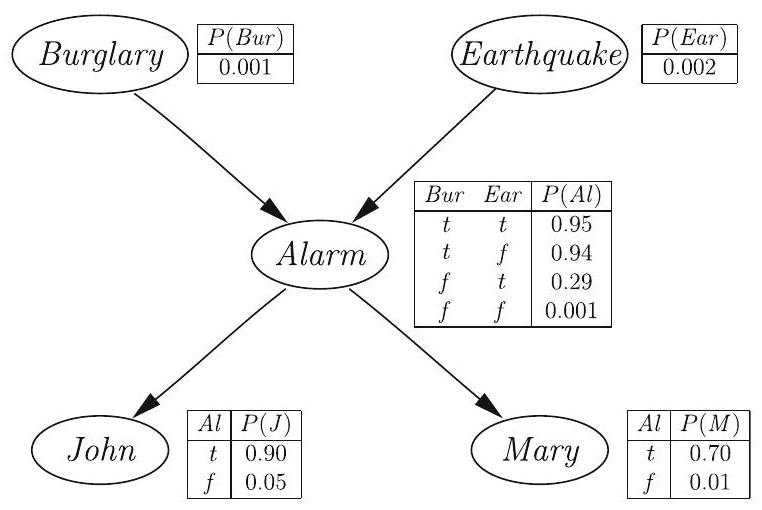
\includegraphics[max width=\textwidth, center]{2025_05_12_af19cd5e0d1b8a465ffeg-165}

This equation is true for all combinations of values for all three variables (that is, for the distribution), which we see in the notation. We now look at nodes $J$ and $M$ in the alarm example, which have the common parent node Al. If John and Mary independently react to an alarm, then the two variables $J$ and $M$ are independent given Al , that is:

$$
\boldsymbol{P}(J, M \mid A l)=\boldsymbol{P}(J \mid A l) \cdot \boldsymbol{P}(M \mid A l)
$$

If the value of $A l$ is known, for example because an alarm was triggered, then the variables $J$ and $M$ are independent (under the condition $A l=w$ ). Because of the conditional independence of the two variables $J$ and $M$, no edge between these two nodes is added. However, $J$ and $M$ are not independent (see Exercise 7.11 on page 173).

Quite similar is the relationship between the two variables $J$ and Bur, because John does not react to a burglary, rather the alarm. This could be, for example, because of a high wall that blocks his view on Bob's property, but he can still hear the alarm. Thus $J$ and Bur are independent given Al and

$$
\boldsymbol{P}(J, B u r \mid A l)=\boldsymbol{P}(J \mid A l) \cdot \boldsymbol{P}(B u r \mid A l)
$$

Given an alarm, the variables $J$ and Ear, $M$ and Bur, as well as $M$ and Ear are also independent. For computing with conditional independence, the following characterizations, which are equivalent to the above definition, are helpful:

Theorem 7.5 The following equations are pairwise equivalent, which means that each individual equation describes the conditional independence for the variables $A$ and $B$ given $C$.


\begin{align*}
& \boldsymbol{P}(A, B \mid C)=\boldsymbol{P}(A \mid C) \cdot \boldsymbol{P}(B \mid C)  \tag{7.18}\\
& \boldsymbol{P}(A \mid B, C)=\boldsymbol{P}(A \mid C)  \tag{7.19}\\
& \boldsymbol{P}(B \mid A, C)=\boldsymbol{P}(B \mid C) \tag{7.20}
\end{align*}


Proof On one hand, using conditional independence (7.18) we can conclude that

$$
\boldsymbol{P}(A, B, C)=\boldsymbol{P}(A, B \mid C) \boldsymbol{P}(C)=\boldsymbol{P}(A \mid C) \boldsymbol{P}(B \mid C) \boldsymbol{P}(C)
$$

On the other hand, the product rule gives us

$$
\boldsymbol{P}(A, B, C)=\boldsymbol{P}(A \mid B, C) \boldsymbol{P}(B \mid C) \boldsymbol{P}(C)
$$

Thus $\boldsymbol{P}(A \mid B, C)=\boldsymbol{P}(A \mid C)$ is equivalent to (7.18). We obtain (7.20) analogously by swapping $A$ and $B$ in this derivation.

\subsection*{7.4.4 Practical Application}
Now we turn again to the alarm example and show how the Bayesian network in Fig. 7.11 can be used for reasoning. Bob is interested, for example, in the sensitivity of his two alarm reporters John and Mary, that is, in $P(J \mid$ Bur $)$ and $P(M \mid$ Bur $)$. However, the values $P(B u r \mid J)$ and $P(B u r \mid M)$, as well as $P(B u r \mid J, M)$ are even more important to him. We begin with $P(J \mid B u r)$ and calculate


\begin{equation*}
P(J \mid \text { Bur })=\frac{P(J, \text { Bur })}{P(\text { Bur })}=\frac{P(J, \text { Bur }, A l)+P(J, \text { Bur }, \neg A l)}{P(\text { Bur })} \tag{7.21}
\end{equation*}


and


\begin{equation*}
\boldsymbol{P}(J, B u r, A l)=\boldsymbol{P}(J \mid B u r, A l) \boldsymbol{P}(A l \mid B u r) \boldsymbol{P}(B u r)=\boldsymbol{P}(J \mid A l) \boldsymbol{P}(A l \mid B u r) \boldsymbol{P}(B u r), \tag{7.22}
\end{equation*}


where for the last two equations we have used the product rule and the conditional independence of $J$ and Bur given Al. Inserted in (7.21) we obtain


\begin{align*}
P(J \mid B u r) & =\frac{P(J \mid A l) P(A l \mid B u r) P(B u r)+P(J \mid \neg A l) P(\neg A l \mid B u r) P(B u r)}{P(B u r)}  \tag{7.23}\\
& =P(J \mid A l) P(A l \mid B u r)+P(J \mid \neg A l) P(\neg A l \mid B u r) .
\end{align*}


Here $P(A l \mid B u r)$ and $P(\neg A l \mid B u r)$ are missing. Therefore we calculate

$$
\begin{aligned}
P(\text { Al } \mid \text { Bur }) & =\frac{P(\text { Al, Bur })}{P(\text { Bur })}=\frac{P(\text { Al, Bur }, \text { Ear })+P(\text { Al, Bur }, \neg \text { Ear })}{P(\text { Bur })} \\
& =\frac{P(\text { Al } \mid \text { Bur }, \text { Ear }) P(\text { Bur }) P(\text { Ear })+P(\text { Al } \mid \text { Bur }, \neg \text { Ear }) P(\text { Bur }) P(\neg \text { Ear })}{P(\text { Bur })} \\
& =P(\text { Al } \mid \text { Bur }, \text { Ear }) P(\text { Ear })+P(\text { Al } \mid \text { Bur }, \neg \text { Ear }) P(\neg \text { Ear }) \\
& =0.95 \cdot 0.002+0.94 \cdot 0.998=0.94
\end{aligned}
$$

as well as $P(\neg A l \mid B u r)=0.06$ and insert this into (7.23) which gives the result

$$
P(J \mid \text { Bur })=0.9 \cdot 0.94+0.05 \cdot 0.06=0.849 .
$$

Analogously we calculate $P(M \mid B u r)=0.659$. We now know that John calls for about $85 \%$ of all break-ins and Mary for about $66 \%$ of all break-ins. The probability that both of them call is calculated, due to conditional independence, as

$$
\begin{aligned}
P(J, M \mid \text { Bur }) & =P(J, M \mid A l) P(A l \mid \text { Bur })+P(J, M \mid \neg A l) P(\neg A l \mid \text { Bur }) \\
& =P(J \mid A l) P(M \mid A l) P(\text { Al } \mid \text { Bur })+P(J \mid \neg A l) P(M \mid \neg A l) P(\neg A l \mid B u r) \\
& =0.9 \cdot 0.7 \cdot 0.94+0.05 \cdot 0.01 \cdot 0.06=0.5922 .
\end{aligned}
$$

More interesting, however, is the probability of a call from John or Mary

$$
\begin{aligned}
& P(J \vee M \mid \text { Bur })=P(\neg(\neg J, \neg M) \mid \text { Bur })=1-P(\neg J, \neg M \mid \text { Bur }) \\
& \quad=1-[P(\neg J \mid A l) P(\neg M \mid A l) P(\text { Al } \mid \text { Bur })+P(\neg J \mid \neg A l) P(\neg M \mid \neg A l) P(\neg A l \mid \text { Bur })] \\
& \quad=1-[0.1 \cdot 0.3 \cdot 0.94+0.95 \cdot 0.99 \cdot 0.06]=1-0.085=0.915 .
\end{aligned}
$$

Bob thus receives a notification for about $92 \%$ of all burglaries. Now to calculate $P(B u r \mid J)$, we apply Bayes' theorem, which gives us

$$
P(B u r \mid J)=\frac{P(J \mid B u r) P(B u r)}{P(J)}=\frac{0.849 \cdot 0.001}{0.052}=0.016 .
$$

Evidently only about $1.6 \%$ of all calls from John are actually due to a break-in. Because the probability of false alarms is five times smaller for Mary, with $P(\operatorname{Bur} \mid M)=0.056$, we have significantly higher confidence given a call from Mary. Bob should only be seriously concerned about his home if both of them call, because $P(B u r \mid J, M)=0.284$ (see Exercise 7.11 on page 173).

In (7.23) on page 162 we showed with

$$
P(J \mid \text { Bur })=P(J \mid A l) P(\text { Al } \mid \text { Bur })+P(J \mid \neg A l) P(\neg A l \mid \text { Bur })
$$

how we can "slide in" a new variable. This relationship holds in general for two variables $A$ and $B$ given the introduction of an additional variable $C$ and is called conditioning:

$$
P(A \mid B)=\sum_{c} P(A \mid B, C=c) P(C=c \mid B) .
$$

If furthermore $A$ and $B$ are conditionally independent given $C$, this formula simplifies to

$$
P(A \mid B)=\sum_{c} P(A \mid C=c) P(C=c \mid B) .
$$

\subsection*{7.4.5 Software for Bayesian Networks}
We will give a brief introduction to two tools using the alarm example. We are already familiar with the system PIT. We input the values from the CPTs in PIT syntax into the online input window at \href{http://www.pit-systems.de}{www.pit-systems.de}. After the input shown in Fig. 7.12 on page 164 we receive the answer:

\begin{verbatim}
P([Einbruch=t] | [John=t] AND [Mary=t]) = 0.2841.
\end{verbatim}

\begin{verbatim}
var Alarm{t,f}, Burglary{t,f}, Earthquake{t,f}, John{t,f}, Mary{t,f};
P([Earthquake=t]) = 0.002;
P([Burglary=t]) = 0.001;
P([Alarm=t] | [Burglary=t] AND [Earthquake=t]) = 0.95;
P([Alarm=t] | [Burglary=t] AND [Earthquake=f]) = 0.94;
P([Alarm=t] | [Burglary=f] AND [Earthquake=t]) = 0.29;
P([Alarm=t] | [Burglary=f] AND [Earthquake=f]) = 0.001;
P([John=t] | [Alarm=t]) = 0.90;
P([John=t] | [Alarm=f]) = 0.05;
P([Mary=t] | [Alarm=t]) = 0.70;
P([Mary=t] | [Alarm=f]) = 0.01;
QP([Burglary=t] | [John=t] AND [Mary=t]);
\end{verbatim}

Fig. 7.12 PIT input for the alarm example\\
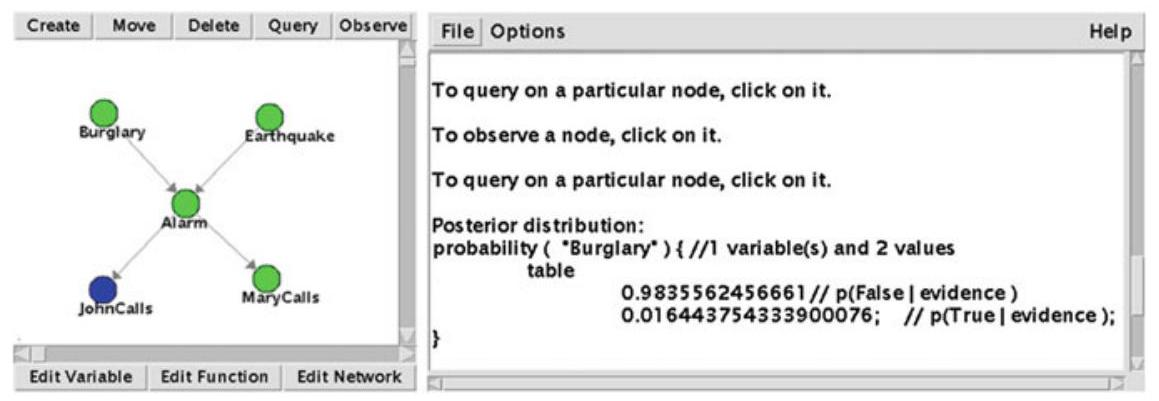
\includegraphics[max width=\textwidth, center]{2025_05_12_af19cd5e0d1b8a465ffeg-169}

Fig. 7.13 The user interface of JavaBayes: left the graphical editor and right the console where the answers are given as output

While PIT is not a classical Bayesian network tool, it can take arbitrary conditional probabilities and queries as input and calculate correct results. It can be shown [Sch96], that on input of CPTs or equivalent rules, the MaxEnt principle implies the same conditional independences and thus also the same answers as a Bayesian network. Bayesian networks are thus a special case of MaxEnt.

Next we will look at JavaBayes [Coz98], a classic system also freely available on the Internet with the graphical interface shown in Fig. 7.13. With the graphical network editor, nodes and edges can be manipulated and the values in the CPTs edited. Furthermore, the values of variables can be assigned with "Observe" and the values of other variables called up with "Query". The answers to queries then appear in the console window.

The professional, commercial system Hugin is significantly more powerful and convenient. For example, Hugin can use continuous variables in addition to discrete variables. It can also learn Bayesian networks, that is, generate the network fully automatically from statistical data (see Sect. 8.5).

\subsection*{7.4.6 Development of Bayesian Networks}
A compact Bayesian network is very clear and significantly more informative for the reader than a full probability distribution. Furthermore, it requires much less memory. For the variables $v_{1}, \ldots, v_{n}$ with $\left|v_{1}\right|, \ldots,\left|v_{n}\right|$ different values each, the distribution has a total of

$$
\prod_{i=1}^{n}\left|v_{i}\right|-1
$$

independent entries. In the alarm example the variables are all binary. Thus for all variables $\left|v_{i}\right|=2$, and the distribution has $2^{5}-1=31$ independent entries. To calculate the number of independent entries for the Bayesian network, the total number of all entries of all CPTs must be determined. For a node $v_{i}$ with $k_{i}$ parent nodes $e_{i 1}, \ldots, e_{i k_{i}}$, the associated CPT has

$$
\left(\left|v_{i}\right|-1\right) \prod_{j=1}^{k_{i}}\left|e_{i j}\right|
$$

entries. Then all CPTs in the network together have


\begin{equation*}
\sum_{i=1}^{n}\left(\left|v_{i}\right|-1\right) \prod_{j=1}^{k_{i}}\left|e_{i j}\right| \tag{7.24}
\end{equation*}


entries. ${ }^{18}$ For the alarm example the result is then

$$
2+2+4+1+1=10
$$

independent entries which uniquely describe the network. The comparison in memory complexity between the full distribution and the Bayesian network becomes clearer when we assume that all $n$ variables have the same number $b$ of values and each node has $k$ parent nodes. Then (7.24) can be simplified and all CPTs together have $n(b-1) b^{k}$ entries. The full distribution contains $b^{n}-1$ entries. A significant gain is only made then if the average number of parent nodes is much smaller than the number of variables. This means that the nodes are only locally connected. Because of the local connection, the network becomes modularized, which-as in software engineering-leads to a reduction in complexity. In the alarm example the alarm node separates the nodes Bur and Ear from the nodes $J$ and $M$. We can also see this clearly in the Lexmed example.

\footnotetext{${ }^{18}$ For the case of a node without ancestors the product in this sum is empty. For this we substitute the value 1 because the CPT for nodes without ancestors contains, with its a priori probability, exactly one value.
}
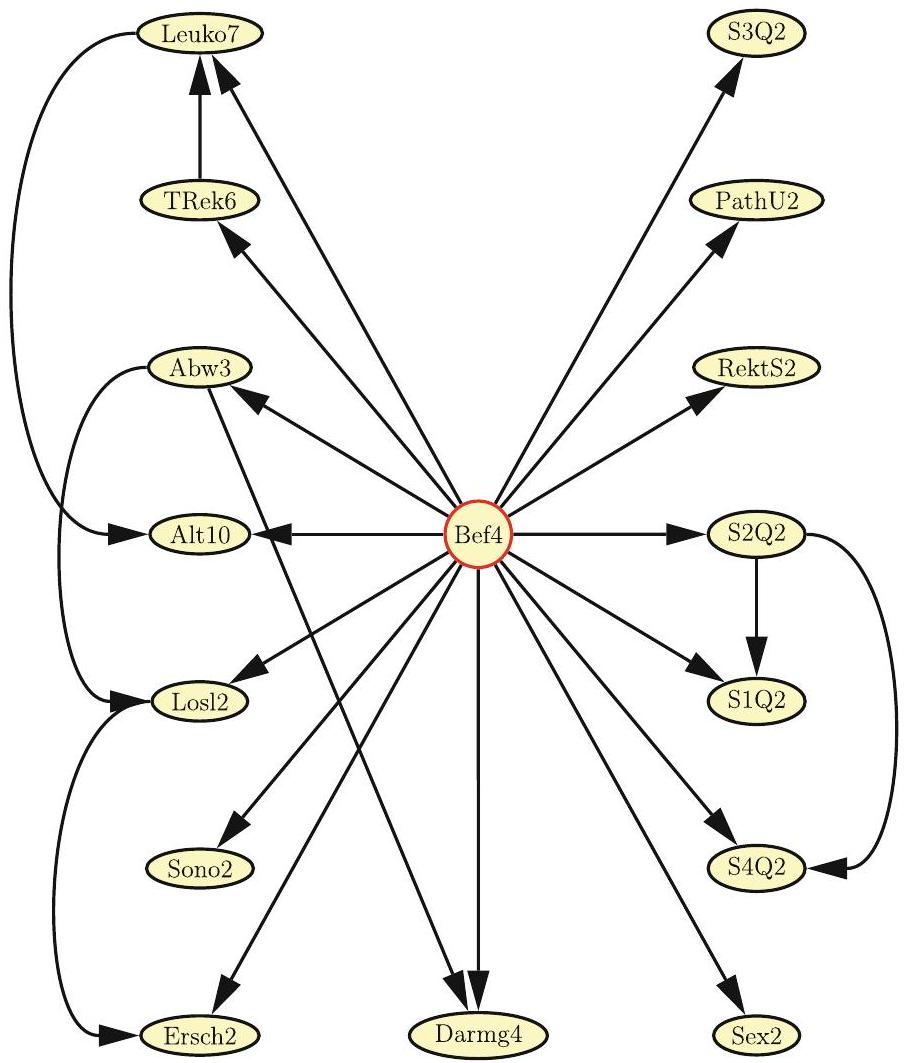
\includegraphics[max width=\textwidth, center]{2025_05_12_af19cd5e0d1b8a465ffeg-171}

Fig. 7.14 Bayesian network for the Lexmed application

\section*{Lexmed as a Bayesian Network}
The Lexmed system described in Sect. 7.3 can also be modeled as a Bayesian network. By making the outer, thinly-drawn lines directed (giving them arrows), the independence graph in Fig. 7.8 on page 151 can be interpreted as a Bayesian network. The resulting network is shown in Fig. 7.14.

In Sect. 7.3.2 the size of the distribution for Lexmed was calculated as the value 20643839 . The Bayesian network on the other hand can be fully described with only 521 values. This value can be determined by entering the variables from Fig. 7.14 into (7.24) on page 165. In the order (Leuko, TRek, Gua, Age, Reb, Sono, Tapp, BowS, Sex, P4Q, P1Q, P2Q, RecP, Urin, P3Q, Diag4) we calculate

$$
\begin{aligned}
\sum_{i=1}^{n}\left(\left|v_{i}\right|-1\right) \prod_{j=1}^{k_{i}}\left|e_{i j}\right|= & 6 \cdot 6 \cdot 4+5 \cdot 4+2 \cdot 4+9 \cdot 7 \cdot 4+1 \cdot 3 \cdot 4+1 \cdot 4+1 \cdot 2 \cdot 4 \\
& +3 \cdot 3 \cdot 4+1 \cdot 4+1 \cdot 4 \cdot 2+1 \cdot 4 \cdot 2+1 \cdot 4+1 \cdot 4+1 \cdot 4 \\
& +1 \cdot 4+1=521
\end{aligned}
$$

This example demonstrates that it is practically impossible to build a full distribution for real applications. A Bayesian network with 22 edges and 521 probability values on the other hand is still manageable.

\section*{Causality and Network Structure}
Construction of a Bayesian network usually proceeds in two stages.

\begin{enumerate}
  \item Design of the network structure: This step is usually performed manually and will be described in the following.
  \item Entering the probabilities in the CPTs: Manually entering the values in the case of many variables is very tedious. If (as for example with Lexmed) a database is available, this step can be automated through estimating the CPT entries by counting frequencies.\\
We will now describe the construction of the network in the alarm example (see Fig. 7.15). At the beginning we know the two causes Burglary and Earthquake and the two symptoms John and Mary. However, because John and Mary do not directly react to a burglar or earthquake, rather only to the alarm, it is appropriate to add this as an additional variable which is not observable by Bob. The process of adding edges starts with the causes, that is, with the variables that have no parent nodes. First we choose Burglary and next Earthquake. Now we must check whether Earthquake is independent of Burglary. This is given, and thus no edge is added from Burglary to Earthquake. Because Alarm is directly dependent on Burglary and Earthquake, these variables are chosen next and an edge is added from both Burglary and Earthquake to Alarm. Then we choose John. Because Alarm and John are not independent, an edge is added from alarm to John. The same is true for Mary. Now we must check whether John is conditionally independent of Burglary given Alarm. If this is not the case, then another edge must be inserted from Burglary to John. We must also check whether edges are needed from Earthquake to John and from Burglary or Earthquake to Mary. Because of conditional independence, these four edges are not necessary. Edges between John and Mary are also unnecessary because John and Mary are conditionally independent given Alarm.
\end{enumerate}

The structure of the Bayesian network heavily depends on the chosen variable ordering. If the order of variables is chosen to reflect the causal relationship beginning with the causes and proceeding to the diagnosis variables, then the result will be a simple network. Otherwise the network may contain significantly more edges. Such non-causal networks are often very difficult to understand and have a higher complexity for reasoning. The reader may refer to Exercise 7.11 on page 173 for better understanding.\\
\includegraphics[max width=\textwidth, center]{2025_05_12_af19cd5e0d1b8a465ffeg-172}

Fig. 7.15 Stepwise construction of the alarm network considering causality\\
\includegraphics[max width=\textwidth, center]{2025_05_12_af19cd5e0d1b8a465ffeg-173}

Fig. 7.16 There is no edge between $A$ and $B$ if they are independent (left) or conditionally independent (middle, right)

\subsection*{7.4.7 Semantics of Bayesian Networks}
As we have seen in the previous section, no edge is added to a Bayesian network between two variables $A$ and $B$ when $A$ and $B$ are independent or conditionally independent given a third variable $C$. This situation is represented in Fig. 7.16.

We now require the Bayesian network to have no cycles and we assume that the variables are numbered such that no variable has a lower number than any variable that precedes it. This is always possible when the network has no cycles. ${ }^{19}$ Then, when using all conditional independencies, we have

$$
\boldsymbol{P}\left(X_{n} \mid X_{1}, \ldots, X_{n-1}\right)=\boldsymbol{P}\left(X_{n} \mid \operatorname{Parents}\left(X_{n}\right)\right) .
$$

This equation thus is a proposition that an arbitrary variable $X_{i}$ in a Bayesian network is conditionally independent of its ancestors, given its parents. The somewhat more general proposition depicted in Fig. 7.17 on page 169 can be stated compactly as

Theorem 7.6 A node in a Bayesian network is conditionally independent from all non-successor nodes, given its parents.

Now we are able to greatly simplify the chain rule ((7.1) on page 132):


\begin{equation*}
\boldsymbol{P}\left(X_{1}, \ldots, X_{n}\right)=\prod_{i=1}^{n} \boldsymbol{P}\left(X_{i} \mid X_{1} \ldots, X_{i-1}\right)=\prod_{i=1}^{n} \boldsymbol{P}\left(X_{i} \mid \operatorname{Parents}\left(X_{i}\right)\right) . \tag{7.25}
\end{equation*}


Using this rule we could, for example, write (7.22) on page 162 directly

$$
\boldsymbol{P}(J, B u r, A l)=\boldsymbol{P}(J \mid A l) \boldsymbol{P}(A l \mid B u r) \boldsymbol{P}(B u r) .
$$

We now know the most important concepts and foundations of Bayesian networks. Let us summarize them [Jen01]:

\footnotetext{${ }^{19}$ If for example three nodes $X_{1}, X_{2}, X_{3}$ form a cycle, then there are the edges $\left(X_{1}, X_{2}\right),\left(X_{2}, X_{3}\right)$ and $\left(X_{3}, X_{1}\right)$ where $X_{1}$ has $X_{3}$ as a successor.
}Fig. 7.17 Example of conditional independence in a Bayesian network. If the parent nodes $E_{1}$ and $E_{2}$ are given, then all non-successor nodes $B_{1}, \ldots, B_{8}$ are independent of $A$\\
\includegraphics[max width=\textwidth, center]{2025_05_12_af19cd5e0d1b8a465ffeg-174}

Definition 7.7 A Bayesian network is defined by:

\begin{itemize}
  \item A set of variables and a set of directed edges between these variables.
  \item Each variable has finitely many possible values.
  \item The variables together with the edges form a directed acyclic graph (DAG). A DAG is a graph without cycles, that is, without paths of the form $(A, \ldots, A)$.
  \item For every variable $A$ the CPT (that is, the table of conditional probabilities $\boldsymbol{P}(A \mid \operatorname{Parents}(A)))$ is given.
\end{itemize}

Two variables $A$ and $B$ are called conditionally independent given $C$ if $\boldsymbol{P}(A, B \mid C)=\boldsymbol{P}(A \mid C) \cdot \boldsymbol{P}(B \mid C)$ or, equivalently, if $\boldsymbol{P}(A \mid B, C)=\boldsymbol{P}(A \mid C)$.\\
Besides the foundational rules of computation for probabilities, the following rules are also true:\\
Bayes' Theorem: $P(A \mid B)=\frac{P(B \mid A) \cdot P(A)}{P(B)}$\\
Marginalization: $P(B)=P(A, B)+P(\neg A, B)=P(B \mid A) \cdot P(A)+P(B \mid \neg A)$.

$$
P(\neg A)
$$

Conditioning: $P(A \mid B)=\sum_{c} P(A \mid B, C=c) P(C=c \mid B)$\\
A variable in a Bayesian network is conditionally independent of all non-successor variables given its parent variables. If $X_{1}, \ldots, X_{n-1}$ are no successors of $X_{n}$, we have $\boldsymbol{P}\left(X_{n} \mid X_{1}, \ldots, X_{n-1}\right)=\boldsymbol{P}\left(X_{n} \mid \operatorname{Parents}\left(X_{n}\right)\right)$. This condition must be honored during the construction of a network.\\
During construction of a Bayesian network the variables should be ordered according to causality. First the causes, then the hidden variables, and the diagnosis variables last.\\
Chain rule: $\boldsymbol{P}\left(X_{1}, \ldots, X_{n}\right)=\prod_{i=1}^{n} \boldsymbol{P}\left(X_{i} \mid \operatorname{Parents}\left(X_{i}\right)\right)$

In [Pea88] and [Jen01] the term d-separation is introduced for Bayesian networks, from which a theorem similar to Theorem 7.6 on page 168 follows. We will refrain from introducing this term and thereby reach a somewhat simpler, though not a theoretically as clean representation.

\subsection*{7.5 Summary}
In a way that reflects the prolonged, sustained trend toward probabilistic systems, we have introduced probabilistic logic for reasoning with uncertain knowledge. After introducing the language-propositional logic augmented with probabilities or probability intervals-we chose the natural, if unusual approach via the method of maximum entropy as an entry point and showed how we can model non-monotonic reasoning with this method. Bayesian networks were then introduced as a special case of the MaxEnt method.

Why are Bayesian networks a special case of MaxEnt? When building a Bayesian network, assumptions about independence are made which are unnecessary for the MaxEnt method. Furthermore, when building a Bayesian network, all CPTs must be completely filled in so that a complete probability distribution can be constructed. Otherwise reasoning is restricted or impossible. With MaxEnt, on the other hand, the developer can formulate all the knowledge he has at his disposal in the form of probabilities. MaxEnt then completes the model and generates the distribution. Even if (for example when interviewing an expert) only vague propositions are available, this can be suitably modeled. A proposition such as "I am pretty sure that $A$ is true." can for example be modeled using $P(A) \in[0.6,1]$ as a probability interval. When building a Bayesian network, a concrete value must be given for the probability, if necessary by guessing. This means, however, that the expert or the developer put ad hoc information into the system. One further advantage of MaxEnt is the possibility of formulating (almost) arbitrary propositions. For Bayesian networks the CPTs must be filled.

The freedom that the developer has when modeling with MaxEnt can be a disadvantage (especially for a beginner) because, in contrast to the Bayesian approach, it is not necessarily clear what knowledge should be modeled. When modeling with Bayesian networks the approach is quite clear: according to causal dependencies, from the causes to the effects, one edge after the other is entered into the network by testing conditional independence. ${ }^{20}$ At the end all CPTs are filled with values.

However, the following interesting combinations of the two methods are possible: we begin by building a network according to the Bayesian methodology, enter all the edges accordingly and then fill the CPTs with values. Should certain values for the CPTs be unavailable, then they can be replaced with intervals or by other probabilistic logic formulas. Naturally such a network-or better: a rule

\footnotetext{${ }^{20}$ This is also not always quite so simple.
}
set-no longer has the special semantics of a Bayesian network. It must then be processed and completed by a MaxEnt system.

The ability to use MaxEnt with arbitrary rule sets has a downside, though. Similarly to the situation in logic, such rule sets can be inconsistent. For example, the two rules $P(A)=0.7$ and $P(A)=0.8$ are inconsistent. While the MaxEnt system PIT for example can recognize the inconsistency, if cannot give a hint about how to remove the problem.

We introduced the medical expert system Lexmed, a classic application for reasoning with uncertain knowledge, and showed how it can be modeled and implemented using MaxEnt and Bayesian networks, and how these tools can replace the well-established, but too weak linear scoring systems used in medicine. ${ }^{21}$

In the Lexmed example we showed that it is possible to build an expert system for reasoning under uncertainty that is capable of discovering (learning) knowledge from the data in a database. We will give more insight into the methods of learning of Bayesian networks in Chap. 8, after the necessary foundations for machine learning have been laid.

Today Bayesian reasoning is a large, independent field, which we can only briefly describe here. We have completely left out the handling of continuous variables. For the case of normally distributed random variables there are procedures and systems. For arbitrary distributions, however, the computational complexity is a big problem. In addition to the directed networks that are heavily based on causality, there are also undirected networks. Connected with this is a discussion about the meaning and usefulness of causality in Bayesian networks. The interested reader is directed to excellent textbooks such as [Pea88, Jen01, Whi96, DHS01], as well as the proceedings of the annual conference of the Association for Uncertainty in Artificial Intelligence (AUAI) (\href{http://www.auai.org}{www.auai.org}).

\subsection*{7.6 Exercises}
Exercise 7.1 Prove the proposition from Theorem 7.1 on page 129.\\
Exercise 7.2 The gardening hobbyist Max wants to statistically analyze his yearly harvest of peas. For every pea pod he picks he measures its length $x_{i}$ in centimeters and its weight $y_{i}$ in grams. He divides the peas into two classes, the good and the bad (empty pods). The measured data ( $x_{i}, y_{i}$ ) are

good peas: $\quad$\textbackslash begin\{tabular\}\{l|lllllllll\}\\
x \& 1 \& 2 \& 2 \& 3 \& 3 \& 4 \& 4 \& 5 \& 6 \\
\\
y \& 2 \& 3 \& 4 \& 4 \& 5 \& 5 \& 6 \& 6 \& 6

$\quad$ bad peas: $\quad$\begin{tabular}{l|llll}
\end{tabular}

x \& 4 \& 6 \& 6 \& 7 \\
\\
\textbackslash hline y \& 2 \& 2 \& 3 \& 3\\
\textbackslash end\{tabular\}

\footnotetext{${ }^{21}$ In Sect. 8.7 and in Exercise 8.17 on page 242 we will show that the scores are equivalent to the special case naive Bayes, that is, to the assumption that all symptoms are conditionally independent given the diagnosis.
}
(a) From the data, compute the probabilities $P(y>3 \mid$ Class $=\operatorname{good})$ and $P(y \leq 3 \mid$ Class $=$ good $)$. Then use Bayes' formula to determine $P($ Class $=\operatorname{good} \mid y>3)$ and $P($ Class $=\operatorname{good} \mid y \leq 3)$.\\
(b) Which of the probabilities computed in subproblem (a) contradicts the statement "All good peas are heavier than 3 grams"?

Exercise 7.3 You are supposed to predict the afternoon weather using a few simple weather values from the morning of this day. The classical probability calculation for this requires a complete model, which is given in the following table.

\begin{center}
\begin{tabular}{llll}
\hline
Sky & Bar & Prec & P(Sky, Bar, Prec ) \\
\hline
Clear & Rising & Dry & 0.40 \\
\hline
Clear & Rising & Raining & 0.07 \\
\hline
Clear & Falling & Dry & 0.08 \\
\hline
Clear & Falling & Raining & 0.10 \\
\hline
Cloudy & Rising & Dry & 0.09 \\
\hline
Cloudy & Rising & Raining & 0.11 \\
\hline
Cloudy & Falling & Dry & 0.03 \\
\hline
\end{tabular}
\end{center}

\begin{center}
\begin{tabular}{ll}
Sky: & \begin{tabular}{l}
The sky is clear or \\
cloudy in the morning \\
\end{tabular} \\
Bar: & \begin{tabular}{l}
Barometer rising or \\
falling in the morning \\
\end{tabular} \\
Prec: & \begin{tabular}{l}
Raining or dry in the \\
afternoon \\
\end{tabular} \\
\end{tabular}
\end{center}

(a) How many events are in the distribution for these three variables?\\
(b) Compute $P($ Prec $=$ dry $\mid$ Sky $=$ clear, $B a r=$ rising $)$.\\
(c) Compute $P($ Prec $=$ rain $\mid$ Sky $=$ cloudy $)$.\\
(d) What would you do if the last row were missing from the table?

\begin{itemize}
  \item Exercise 7.4 In a television quiz show, the contestant must choose between three closed doors. Behind one door the prize awaits: a car. Behind both of the other doors are goats. The contestant chooses a door, e.g. number one. The host, who knows where the car is, opens another door, e.g. number three, and a goat appears. The contestant is now given the opportunity to choose between the two remaining doors (one and two). What is the better choice from his point of view? To stay with the door he originally chose or to switch to the other closed door?
\end{itemize}

Exercise 7.5 Using the Lagrange multiplier method, show that, without explicit constraints, the uniform distribution $p_{1}=p_{2}=\cdots=p_{n}=1 / n$ represents maximum entropy. Do not forget the implicitly ever-present constraint $p_{1}+p_{2}+\cdots+p_{n}=1$. How can we show this same result using indifference?

Exercise 7.6 Use the PIT system (\href{http://www.pit-systems.de}{http://www.pit-systems.de}) or SPIRIT (http:// \href{http://www.xspirit.de}{www.xspirit.de}) to calculate the MaxEnt solution for $P(B)$ under the constraint $P(A)=\alpha$ and $P(B \mid A)=\beta$. Which disadvantage of PIT, compared with calculation by hand, do you notice here?

Exercise 7.7 Given the constraints $P(A)=\alpha$ and $P(A \vee B)=\beta$, manually calculate $P(B)$ using the MaxEnt method. Use PIT to check your solution.

\begin{itemize}
  \item Exercise 7.8 Given the constraints from (7.10), (7.11), (7.12): $p_{1}+p_{2}=\alpha$, $p_{1}+p_{3}=\gamma, p_{1}+p_{2}+p_{3}+p_{4}=1$. Show that $p_{1}=\alpha \gamma, p_{2}=\alpha(1-\gamma), p_{3}=\gamma(1-\alpha)$, $p_{4}=(1-\alpha)(1-\gamma)$ represents the entropy maximum under these constraints.
  \item Exercise 7.9 A probabilistic algorithm calculates the likelihood $p$ that an inbound email is spam. To classify the emails in classes delete and read, a cost matrix is then applied to the result.\\
(a) Give a cost matrix ( $2 \times 2$ matrix) for the spam filter. Assume here that it costs the user 10 cents to delete an email, while the loss of an email costs 10 dollars (compare this to Example 1.1 on page 17 and Exercise 1.7 on page 21).\\
(b) Show that, for the case of a $2 \times 2$ matrix, the application of the cost matrix is equivalent to the application of a threshold on the spam probability and determine the threshold.
\end{itemize}

Exercise 7.10 Given a Bayesian network with the three binary variables $A, B$, $C$ and $P(A)=0.2, P(B)=0.9$, as well as the CPT shown below:\\
(a) Compute $P(A \mid B)$.\\
(b) Compute $P(C \mid A)$.

\begin{center}
\begin{tabular}{llc}
\hline
$A$ & $B$ & $P(C)$ \\
\hline
$t$ & $f$ & 0.1 \\
\hline
$t$ & $t$ & 0.2 \\
\hline
$f$ & $t$ & 0.9 \\
\hline
$f$ & $f$ & 0.4 \\
\hline
\end{tabular}
\end{center}

\begin{center}
\includegraphics[max width=\textwidth]{2025_05_12_af19cd5e0d1b8a465ffeg-178}
\end{center}

Exercise 7.11 For the alarm example (Example 7.10 on page 159), calculate the following conditional probabilities:\\
(a) Calculate the a priori probabilities $P(A l), P(J), P(M)$.\\
(b) Calculate $P(M \mid B u r)$ using the product rule, marginalization, the chain rule, and conditional independence.\\
(c) Use Bayes' formula to calculate $P(B u r \mid M)$\\
(d) Compute $P(A l \mid J, M)$ and $P(B u r \mid J, M)$.\\
(e) Show that the variables $J$ and $M$ are not independent.\\[0pt]
(f) Check all of your results with JavaBayes and with PIT (see [Ert11] for demo programs).\\
(g) Design a Bayesian network for the alarm example, but with the altered variable ordering M, Al, Ear, Bur, J. According to the semantics of Bayesian networks, only the necessary edges must be drawn in. (Hint: the variable order given here does NOT represent causality. Thus it will be difficult to intuitively determine conditional independences.)\\
(h) In the original Bayesian network of the alarm example, the earthquake nodes is removed. Which CPTs does this change? (Why these in particular?)\\
(i) Calculate the CPT of the alarm node in the new network.

Exercise 7.12 A diagnostic system is to be made for a dynamo-powered bicycle light using a Bayesian network. The variables in the following table are given.

\begin{center}
\begin{tabular}{|l|l|l|}
\hline
Abbr. & Meaning & Values \\
\hline
Li & Light is on & $t / f$ \\
\hline
Str & Street condition & dry, wet, snow\_covered \\
\hline
Flw & Dynamo flywheel worn out & $t / f$ \\
\hline
R & Dynamo sliding & $t / f$ \\
\hline
V & Dynamo shows voltage & $t / f$ \\
\hline
B & Light bulb o.k. & $t / f$ \\
\hline
K & Cable o.k. & $t / f$ \\
\hline
\end{tabular}
\end{center}

The following variables are pairwise independent: Str, Flw, B, K. Furthermore: $(R, B),(R, K),(V, B)$, $(V, K)$ are independent and the following equation holds:

$$
\begin{aligned}
P(L i \mid V, R) & =P(L i \mid V) \\
P(V \mid R, S t r) & =P(V \mid R) \\
P(V \mid R, F l w) & =P(V \mid R)
\end{aligned}
$$

\includegraphics[max width=\textwidth, center]{2025_05_12_af19cd5e0d1b8a465ffeg-179}\\
(a) Draw all of the edges into the graph (taking causality into account).\\
(b) Enter all missing CPTs into the graph (table of conditional probabilities). Freely insert plausible values for the probabilities.\\
(c) Show that the network does not contain an edge (Str, Li).\\
(d) Compute $P(V \mid S t r=$ snow\_covered $)$.

\begin{center}
\begin{tabular}{llll}
\hline
$V$ & $B$ & $K$ & $P(L i)$ \\
\hline
$t$ & $t$ & $t$ & 0.99 \\
\hline
$t$ & $t$ & $f$ & 0.01 \\
\hline
$t$ & $f$ & $t$ & 0.01 \\
\hline
$t$ & $f$ & $f$ & 0.001 \\
\hline
$f$ & $t$ & $t$ & 0.3 \\
\hline
$f$ & $t$ & $f$ & 0.005 \\
\hline
$f$ & $f$ & $t$ & 0.005 \\
\hline
$f$ & $f$ & $f$ & 0 \\
\hline
\end{tabular}
\end{center}

\section*{Machine Learning and Data Mining}
If we define AI as is done in Elaine Rich's book [Ric83]:\\
Artificial Intelligence is the study of how to make computers do things at which, at the moment, people are better.\\
and if we consider that the computer's learning ability is especially inferior to that of humans, then it follows that research into learning mechanisms, and the development of machine learning algorithms is one of the most important branches of AI.

There is also demand for machine learning from the viewpoint of the software developer who programs, for example, the behavior of an autonomous robot. The structure of the intelligent behavior can become so complex that it is very difficult or even impossible to program close to optimally, even with modern high-level languages such as PROLOG and Python. ${ }^{1}$ Machine learning algorithms are even used today to program robots in a way similar to how humans learn (see Chap. 10 or [BCDS08, RGH+06]), often in a hybrid mixture of programmed and learned behavior.

The task of this chapter is to describe the most important machine learning algorithms and their applications. The topic will be introduced in this section, followed by important fundamental learning algorithms in the next sections. Theory and terminology will be built up in parallel to this. The chapter will close with a summary and overview of the various algorithms and their applications. We will restrict ourselves in this chapter to supervised and unsupervised learning algorithms. As an important class of learning algorithms, neural networks will be dealt with in Chap. 9. Due to its special place and important role for autonomous robots, reinforcement learning will also have its own dedicated chapter (Chap. 10).

\footnotetext{${ }^{1}$ Python is a modern scripting language with very readable syntax, powerful data types, and extensive standard libraries, which can be used to this end.
}
\includegraphics[max width=\textwidth, center]{2025_05_12_af19cd5e0d1b8a465ffeg-181}

Fig. 8.1 Supervised learning ...

What Is Learning? Learning vocabulary of a foreign language, or technical terms, or even memorizing a poem can be difficult for many people. For computers, however, these tasks are quite simple because they are little more than saving text in a file. Thus memorization is uninteresting for AI. In contrast, the acquisition of mathematical skills is usually not done by memorization. For addition of natural numbers this is not at all possible, because for each of the terms in the sum $x+y$ there are infinitely many values. For each combination of the two values $x$ and $y$, the triple ( $x, y, x+y$ ) would have to be stored, which is impossible. For decimal numbers, this is downright impossible. This poses the question: how do we learn mathematics? The answer reads: The teacher explains the process and the students practice it on examples until they no longer make mistakes on new examples. After 50 examples the student (hopefully) understands addition. That is, after only 50 examples he can apply what was learned to infinitely many new examples, which to that point were not seen. This process is known as generalization. We begin with a simple example.

Example 8.1 A fruit farmer wants to automatically divide harvested apples into the merchandise classes A and B. The sorting device is equipped with sensors to measure two features, size and color, and then decide which of the two classes the apple belongs to. This is a typical classification task. Systems which are capable of dividing feature vectors into a finite number of classes are called classifiers.

To configure the machine, apples are hand-picked by a specialist, that is, they are classified. Then the two measurements are entered together with their class

Table 8.1 Training data for the apple sorting agent

\begin{center}
\begin{tabular}{llllll}
\hline
Size $[\mathrm{cm}]$ & 8 & 8 & 6 & 3 & $\ldots$ \\
\hline
Color & 0.1 & 0.3 & 0.9 & 0.8 & $\ldots$ \\
\hline
Merchandise class & B & A & A & B & $\ldots$ \\
\hline
\end{tabular}
\end{center}

\begin{center}
\includegraphics[max width=\textwidth]{2025_05_12_af19cd5e0d1b8a465ffeg-182(1)}
\end{center}

Fig. 8.2 BayWa company apple sorting equipment in Kressbronn and some apples classified into merchandise classes A and B in feature space (Photo: BayWa)

Fig. 8.3 The curve drawn in into the diagram divides the classes and can then be applied to arbitrary new apples\\
\includegraphics[max width=\textwidth, center]{2025_05_12_af19cd5e0d1b8a465ffeg-182}\\
label in a table (Table 8.1. The size is given in the form of diameter in centimeters and the color by a numeric value between 0 (for green) and 1 (for red). A visualization of the data is listed as points in a scatterplot diagram in the right of Fig. 8.2.

The task in machine learning consists of generating a function from the collected, classified data which calculates the class value (A or B) for a new apple from the two features size and color. In Fig. 8.3 such a function is shown by the dividing line drawn through the diagram. All apples with a feature vector to the bottom left of the line are put into class B, and all others into class A.

In this example it is still very simple to find such a dividing line for the two classes. It is clearly a more difficult, and above all much less visualizable task, when the objects to be classified are described by not just two, but many features. In practice 30 or more features are usually used. For $n$ features, the task consists of finding an $n-1$ dimensional hyperplane within the $n$-dimensional feature space\\
\includegraphics[max width=\textwidth, center]{2025_05_12_af19cd5e0d1b8a465ffeg-183}

Fig. 8.4 Functional structure of a learning agent for apple sorting (left) and in general (right)\\
which divides the classes as well as possible. A "good" division means that the percentage of falsely classified objects is as small as possible.

A classifier maps a feature vector to a class value. Here it has a fixed, usually small, number of alternatives. The desired mapping is also called target function. If the target function does not map onto a finite domain, then it is not a classification, but rather an approximation problem. Determining the market value of a stock from given features is such an approximation problem. In the following sections we will introduce several learning agents for both types of mappings.

The Learning Agent We can formally describe a learning agent as a function which maps a feature vector to a discrete class value or in general to a real number. This function is not programmed, rather it comes into existence or changes itself during the learning phase, influenced by the training data. In Fig. 8.4 such an agent is presented in the apple sorting example. During learning, the agent is fed with the already classified data from Table 8.1 on page 177. Thereafter the agent constitutes as good a mapping as possible from the feature vector to the function value (e.g. merchandise class).

We can now attempt to approach a definition of the term "machine learning". Tom Mitchell [Mit97] gives this definition:

Machine Learning is the study of computer algorithms that improve automatically through experience.

Drawing on this, we give

Definition 8.1 An agent is a learning agent if it improves its performance (measured by a suitable criterion) on new, unknown data over time (after it has seen many training examples).

It is important to test the generalization capability of the learning algorithm on unknown data, the test data. Otherwise every system that just saved the training data would appear to perform optimally just by calling up the saved data. A learning agent is characterized by the following terms:\\
Task: the task of the learning algorithm is to learn a mapping. This could for example be the mapping from an apple's size and color to its merchandise class,\\
\includegraphics[max width=\textwidth, center]{2025_05_12_af19cd5e0d1b8a465ffeg-184}

Fig. 8.5 Data Mining\\
but also the mapping from a patient's 15 symptoms to the decision of whether or not to remove his appendix.\\
Variable agent: (more precisely a class of agents): here we have to decide which learning algorithm will be worked with. If this has been chosen, thus the class of all learnable functions is determined.\\
Training data: (experience): the training data (sample) contain the knowledge which the learning algorithm is supposed to extract and learn. With the choice of training data one must ensure that it is a representative sample for the task to be learned.\\
Test data: important for evaluating whether the trained agent can generalize well from the training data to new data.\\
Performance measure: for the apple sorting device, the number of correctly classified apples. We need it to test the quality of an agent. Knowing the performance measure is usually much easier than knowing the agent's function. For example, it is easy to measure the performance (time) of a 10,000 meter runner. However, this does not at all imply that the referee who measures the time can run as fast. The referee only knows how to measure the performance, but not the "function" of the agent whose performance he is measuring.

What Is Data Mining? The task of a learning machine to extract knowledge from training data. Often the developer or the user wants the learning machine to make the extracted knowledge readable for humans as well. It is still better if the\\
developer can even alter the knowledge. The process of induction of decision trees in Sect. 8.4 is an example of this type of method.

Similar challenges come from electronic business and knowledge management. A classic problem presents itself here: from the actions of visitors to his web portal, the owner of an Internet business would like to create a relationship between the characteristics of a customer and the class of products which are interesting to that customer. Then a seller will be able to place customer-specific advertisements. This is demonstrated in a telling way at \href{http://www.amazon.com}{www.amazon.com}, where the customer is recommended products which are similar to those seen in the previous visit. In many areas of advertisement and marketing, as well as in customer relationship management (CRM), data mining techniques are coming into use. Whenever large amounts of data are available, one can attempt to use these data for the analysis of customer preferences in order to show customer-specific advertisements. The emerging field of preference learning is dedicated to this purpose.

The process of acquiring knowledge from data, as well as its representation and application, is called data mining. The methods used are usually taken from statistics or machine learning and should be applicable to very large amounts of data at reasonable cost.

In the context of acquiring information, for example on the Internet or in an intranet, text mining plays an increasingly important role. Typical tasks include finding similar text in a search engine or the classification of texts, which for example is applied in spam filters for email. In Sect. 8.7.1 we will introduce the widespread naive Bayes algorithm for the classification of text. A relatively new challenge for data mining is the extraction of structural, static, and dynamic information from graph structures such as social networks, traffic networks, or Internet traffic.

Because the two described tasks of machine learning and data mining are formally very similar, the basic methods used in both areas are for the most part identical. Therefore in the description of the learning algorithms, no distinction will be made between machine learning and data mining.

Because of the huge commercial impact of data mining techniques, there are now many sophisticated optimizations and a whole line of powerful data mining systems, which offer a large palette of convenient tools for the extraction of knowledge from data. Such a system is introduced in Sect. 8.10.

\subsection*{8.1 Data Analysis}
Statistics provides a number of ways to describe data with simple parameters. From these we choose a few which are especially important for the analysis of training data and test these on a subset of the Lexmed data from Sect. 7.3. In this example dataset, the symptoms $x_{1}, \ldots, x_{15}$ of $N=473$ patients, concisely described in

Table 8.2 Description of variables $x_{1}, \ldots, x_{16}$. A slightly different formalization was used in Table 7.2 on page 147

\begin{center}
\begin{tabular}{|l|l|l|}
\hline
Var. num. & Description & Values \\
\hline
1 & Age & Continuous \\
\hline
2 & Sex ( $1=$ male, $2=$ female) & 1, 2 \\
\hline
3 & Pain quadrant 1 & 0,1 \\
\hline
4 & Pain quadrant 2 & 0,1 \\
\hline
5 & Pain quadrant 3 & 0,1 \\
\hline
6 & Pain quadrant 4 & 0,1 \\
\hline
7 & Local muscular guarding & 0,1 \\
\hline
8 & Generalized muscular guarding & 0,1 \\
\hline
9 & Rebound tenderness & 0,1 \\
\hline
10 & Pain on tapping & 0,1 \\
\hline
11 & Pain during rectal examination & 0,1 \\
\hline
12 & Axial temperature & Continuous \\
\hline
13 & Rectal temperature & Continuous \\
\hline
14 & Leukocytes & Continuous \\
\hline
15 & Diabetes mellitus & 0,1 \\
\hline
16 & Appendicitis & 0,1 \\
\hline
\end{tabular}
\end{center}

Table 8.2 on page 181, as well as the class label-that is, the diagnosis (appendicitis positive/negative)-are listed. Patient number one, for example, is described by the vector

$$
x^{1}=(26,1,0,0,1,0,1,0,1,1,0,37.9,38.8,23100,0,1)
$$

and patient number two by

$$
\boldsymbol{x}^{2}=(17,2,0,0,1,0,1,0,1,1,0,36.9,37.4,8100,0,0)
$$

Patient number two has the leukocyte value $x_{14}^{2}=8100$.\\
For each variable $x_{i}$, its average $\bar{x}_{i}$ is defined as

$$
\bar{x}_{i}:=\frac{1}{N} \sum_{p=1}^{N} x_{i}^{p}
$$

and the standard deviation $s_{i}$ as a measure of its average deviation from the average value as

$$
s_{i}:=\sqrt{\frac{1}{N-1} \sum_{p=1}^{N}\left(x_{i}^{p}-\bar{x}_{i}\right)^{2}} .
$$

The question of whether two variables $x_{i}$ and $x_{j}$ are statistically dependent (correlated) is important for the analysis of multidimensional data. For example, the covariance

Table 8.3 Correlation matrix for the 16 appendicitis variables measured in 473 cases

\begin{center}
\begin{tabular}{|l|l|l|l|l|l|l|l|l|l|l|l|l|l|l|l|}
\hline
1. & -0.009 & 0.14 & 0.037 & -0.096 & 0.12 & 0.018 & 0.051 & -0.034 & -0.041 & 0.034 & 0.037 & 0.05 & -0.037 & 0.37 & 0.012 \\
\hline
-0.009 & 1. & -0.0074 & -0.019 & -0.06 & 0.063 & -0.17 & 0.0084 & -0.17 & -0.14 & -0.13 & -0.017 & -0.034 & -0.14 & 0.045 & -0.2 \\
\hline
0.14 & -0.0074 & 1. & 0.55 & -0.091 & 0.24 & 0.13 & 0.24 & 0.045 & 0.18 & 0.028 & 0.02 & 0.045 & 0.03 & 0.11 & 0.045 \\
\hline
0.037 & -0.019 & 0.55 & 1. & -0.24 & 0.33 & 0.051 & 0.25 & 0.074 & 0.19 & 0.087 & 0.11 & 0.12 & 0.11 & 0.14 & -0.0091 \\
\hline
-0.096 & -0.06 & -0.091 & -0.24 & 1. & 0.059 & 0.14 & 0.034 & 0.14 & 0.049 & 0.057 & 0.064 & 0.058 & 0.11 & 0.017 & 0.14 \\
\hline
0.12 & 0.063 & 0.24 & 0.33 & 0.059 & 1. & 0.071 & 0.19 & 0.086 & 0.15 & 0.048 & 0.11 & 0.12 & 0.063 & 0.21 & 0.053 \\
\hline
0.018 & -0.17 & 0.13 & 0.051 & 0.14 & 0.071 & 1. & 0.16 & 0.4 & 0.28 & 0.2 & 0.24 & 0.36 & 0.29 & -0.0001 & 0.33 \\
\hline
0.051 & 0.0084 & 0.24 & 0.25 & 0.034 & 0.19 & 0.16 & 1. & 0.17 & 0.23 & 0.24 & 0.19 & 0.24 & 0.27 & 0.083 & 0.084 \\
\hline
-0.034 & -0.17 & 0.045 & 0.074 & 0.14 & 0.086 & 0.4 & 0.17 & 1. & 0.53 & 0.25 & 0.19 & 0.27 & 0.27 & 0.026 & 0.38 \\
\hline
-0.041 & -0.14 & 0.18 & 0.19 & 0.049 & 0.15 & 0.28 & 0.23 & 0.53 & 1. & 0.24 & 0.15 & 0.19 & 0.23 & 0.02 & 0.32 \\
\hline
0.034 & -0.13 & 0.028 & 0.087 & 0.057 & 0.048 & 0.2 & 0.24 & 0.25 & 0.24 & 1. & 0.17 & 0.17 & 0.22 & 0.098 & 0.17 \\
\hline
0.037 & -0.017 & 0.02 & 0.11 & 0.064 & 0.11 & 0.24 & 0.19 & 0.19 & 0.15 & 0.17 & 1. & 0.72 & 0.26 & 0.035 & 0.15 \\
\hline
0.05 & -0.034 & 0.045 & 0.12 & 0.058 & 0.12 & 0.36 & 0.24 & 0.27 & 0.19 & 0.17 & 0.72 & 1. & 0.38 & 0.044 & 0.21 \\
\hline
-0.037 & -0.14 & 0.03 & 0.11 & 0.11 & 0.063 & 0.29 & 0.27 & 0.27 & 0.23 & 0.22 & 0.26 & 0.38 & 1. & 0.051 & 0.44 \\
\hline
0.37 & 0.045 & 0.11 & 0.14 & 0.017 & 0.21 & -0.0001 & 0.083 & 0.026 & 0.02 & 0.098 & 0.035 & 0.044 & 0.051 & 1. & -0.0055 \\
\hline
0.012 & -0.2 & 0.045 & -0.0091 & 0.14 & 0.053 & 0.33 & 0.084 & 0.38 & 0.32 & 0.17 & 0.15 & 0.21 & 0.44 & -0.0055 & 1. \\
\hline
\end{tabular}
\end{center}

$$
\sigma_{i j}=\frac{1}{N-1} \sum_{p=1}^{N}\left(x_{i}^{p}-\bar{x}_{i}\right)\left(x_{j}^{p}-\bar{x}_{j}\right)
$$

gives information about this. In this sum, the summand returns a positive entry for the $p$ th data vector exactly when the deviations of the $i$ th and $j$ th components from the average both have the same sign. If they have different signs, then the entry is negative. Therefore the covariance $\sigma_{12,13}$ of the two different fever values should be quite clearly positive.

However, the covariance also depends on the absolute value of the variables, which makes comparison of the values difficult. To be able to compare the degree of dependence in the case of multiple variables, we therefore define the correlation coefficient

$$
K_{i j}=\frac{\sigma_{i j}}{s_{i} \cdot s_{j}}
$$

for two values $x_{i}$ and $x_{j}$, which is nothing but a normalized covariance. The matrix $\boldsymbol{K}$ of all correlation coefficients contains values between -1 and 1 , is symmetric, and all of its diagonal elements have the value 1 . The correlation matrix for all 16 variables is given in Table 8.3.

This matrix becomes somewhat more readable when we represent it as a density plot. Instead of the numerical values, the matrix elements in Fig. 8.6 on page 183 are filled with gray values. In the right diagram, the absolute values are shown. Thus we can very quickly see which variables display a weak or strong dependence. We can see, for example, that the variables $7,9,10$ and 14 show the strongest correlation with the class variable appendicitis and therefore are more important for the diagnosis than the other variable. We also see, however, that the variables 9 and 10 are strongly correlated. This could mean that one of these two values is potentially sufficient for the diagnosis.\\
\includegraphics[max width=\textwidth, center]{2025_05_12_af19cd5e0d1b8a465ffeg-188(1)}

Fig. 8.6 The correlation matrix as a frequency graph. In the left diagram, dark stands for negative and light for positive. In the right image the absolute values were listed. Here black means $K_{i j} \approx 0$ (uncorrelated) and white $\left|K_{i j}\right| \approx 1$ (strongly correlated)

Fig. 8.7 A linearly separable two dimensional data set. The equation for the dividing straight line is $a_{1} x_{1}+a_{2} x_{2}=1$\\
\includegraphics[max width=\textwidth, center]{2025_05_12_af19cd5e0d1b8a465ffeg-188}

\subsection*{8.2 The Perceptron, a Linear Classifier}
In the apple sorting classification example, a curved dividing line is drawn between the two classes in Fig. 8.3 on page 177. A simpler case is shown in Fig. 8.7. Here the two-dimensional training examples can be separated by a straight line. We call such a set of training data linearly separable. In $n$ dimensions a hyperplane is needed for the separation. This represents a linear subspace of dimension $n-1$.

Because every ( $n-1$ )-dimensional hyperplane in $\mathbb{R}^{n}$ can be described by an equation

$$
\sum_{i=1}^{n} a_{i} x_{i}=\theta
$$

it makes sense to define linear separability as follows.\\
\includegraphics[max width=\textwidth, center]{2025_05_12_af19cd5e0d1b8a465ffeg-189}

Fig. 8.8 The boolean function AND is linearly separable, but XOR is not ( $0 \hat{=}$ true, $0 \hat{=}$ false)

Definition 8.2 Two sets $M_{1} \subset \mathbb{R}^{n}$ and $M_{2} \subset \mathbb{R}^{n}$ are called linearly separable if real numbers $a_{1}, \ldots, a_{n}, \theta$ exist with

$$
\sum_{i=1}^{n} a_{i} x_{i}>\theta \quad \text { for all } \boldsymbol{x} \in M_{1} \quad \text { and } \quad \sum_{i=1}^{n} a_{i} x_{i} \leq \theta \quad \text { for all } \boldsymbol{x} \in M_{2}
$$

The value $\theta$ is denoted the threshold.

In Fig. 8.8 we see that the AND function is linearly separable, but the XOR function is not. For AND, for example, the line $-x_{1}+3 / 2$ separates true and false interpretations of the formula $x_{1} \wedge x_{2}$. In contrast, the XOR function does not have a straight line of separation. Clearly the XOR function has a more complex structure than the AND function in this regard.

With the perceptron, we present a very simple learning algorithm which can separate linearly separable sets.

Definition 8.3 Let $\boldsymbol{w}=\left(w_{1}, \ldots, w_{n}\right) \in \mathbb{R}^{n}$ be a weight vector and $\boldsymbol{x} \in \mathbb{R}^{n}$ an input vector. A perceptron represents a function $P: \mathbb{R}^{n} \rightarrow\{0,1\}$ which corresponds to the following rule:

$$
P(\boldsymbol{x})= \begin{cases}1 & \text { if } \boldsymbol{w} x=\sum_{i=1}^{n} w_{i} x_{i}>0 \\ 0 & \text { else }\end{cases}
$$

The perceptron [Ros58, MP69] is a very simple classification algorithm. It is equivalent to a two-layer neural network with activation by a threshold function, shown in Fig. 8.9 on page 185. As shown in Chap. 9, each node in the network represents a neuron, and every edge a synapse. For now, however, we will only view

Fig. 8.9 Graphical representation of a perceptron as a two-layer neural network\\
\includegraphics[max width=\textwidth, center]{2025_05_12_af19cd5e0d1b8a465ffeg-190}\\
the perceptron as a learning agent, that is, as a mathematical function which maps a feature vector to a function value. Here the input variables $x_{i}$ are denoted features.

As we can see in the formula $\sum_{i=1}^{n} w_{i} x_{i}>0$, all points $\boldsymbol{x}$ above the hyperplane $\sum_{i=1}^{n} w_{i} x_{i}=0$ are classified as positive ( $P(\boldsymbol{x})=1$ ), and all others as negative $P(\boldsymbol{x})=0$. The separating hyperplane goes through the origin because $\theta=0$. We will use a little trick to show that the absence of an arbitrary threshold represents no restriction of power. First, however, we want to introduce a simple learning algorithm for the perceptron.

\subsection*{8.2.1 The Learning Rule}
With the notation $M_{+}$and $M_{-}$for the sets of positive and negative training patterns respectively, the perceptron learning rule reads [MP69]

PerceptronLearning $\left[M_{+}, M_{-}\right]$ $\boldsymbol{w}=$ arbitrary vector of real numbers\\
Repeat\\
For all $x \in M_{+}$\\
If $w x \leq 0$ Then $w=w+x$\\
For all $x \in M_{-}$\\
If $w x>0$ Then $w=w-x$\\
Until all $x \in M_{+} \cup M_{-}$are correctly classified

The perceptron should output the value 1 for all $\boldsymbol{x} \in M_{+}$. By Definition 8.3 on page 184 this is true when $\boldsymbol{w} \boldsymbol{x}>0$. If this is not the case then $\boldsymbol{x}$ is added to the weight vector $\boldsymbol{w}$, whereby the weight vector is changed in exactly the right direction. We see this when we apply the perceptron to the changed vector $\boldsymbol{w}+\boldsymbol{x}$ because

$$
(w+x) \cdot x=w x+x^{2} .
$$

If this step is repeated often enough, then at some point the value $\boldsymbol{w} \boldsymbol{x}$ will become positive, as it should be. Analogously, we see that, for negative training data, the perceptron calculates an ever smaller value

$$
(w-x) \cdot x=w x-x^{2}
$$

which at some point becomes negative. ${ }^{2}$\\
Example 8.2 A perceptron is to be trained on the sets $M_{+}=\{(0,1.8),(2,0.6)\}$ and $M_{-}=\{(-1.2,1.4),(0.4,-1)\} . \boldsymbol{w}=(1,1)$ was used as an initial weight vector. The training data and the line defined by the weight vector $\boldsymbol{w} \boldsymbol{x}=x_{1}+x_{2}=0$ are shown in Fig. 8.10 on page 187 in the first picture in the top row. In addition, the weight vector is drawn as a dashed line. Because $\boldsymbol{w} \boldsymbol{x}=0$, this is orthogonal to the line.

In the first iteration through the loop of the learning algorithm, the only falsely classified training example is $(-1.2,1.4)$ because

$$
(-1.2,1.4) \cdot\binom{1}{1}=0.2>0
$$

This results in $\boldsymbol{w}=(1,1)-(-1.2,1.4)=(2.2,-0.4)$, as drawn in the second image in the top row in Fig. 8.10 on page 187. The other images show how, after a total of five changes, the dividing line lies between the two classes. The perceptron thus classifies all data correctly. We clearly see in the example that every incorrectly classified data point from $M_{+}$"pulls" the weight vector $\boldsymbol{w}$ in its direction and every incorrectly classified point from $M_{-}$"pushes" the weight vector in the opposite direction.

It has been shown [MP69] that the perceptron always converges for linearly separable data. We have

Theorem 8.1 Let classes $M_{+}$and $M_{-}$be linearly separable by a hyperplane $\boldsymbol{w} \boldsymbol{x}=0$. Then PerceptronLearning converges for every initialization of the vector $w$. The perceptron $P$ with the weight vector so calculated divides the classes $M_{+}$and $M_{-}$, that is:

$$
P(\boldsymbol{x})=1 \quad \Leftrightarrow \quad \boldsymbol{x} \in \boldsymbol{M}_{+}
$$

and

$$
P(x)=0 \quad \Leftrightarrow \quad x \in M_{-} .
$$

As we can clearly see in Example 8.2, perceptrons as defined above cannot divide arbitrary linearly separable sets, rather only those which are divisible by a line through the origin, or in $\mathbb{R}^{n}$ by a hyperplane through the origin, because the constant term $\theta$ is missing from the equation $\sum_{i=1}^{n} w_{i} x_{i}=0$.

\footnotetext{${ }^{2}$ Caution! This is not a proof of convergence for the perceptron learning rule. It only shows that the perceptron converges when the training dataset consists of a single example.
}
\includegraphics[max width=\textwidth, center]{2025_05_12_af19cd5e0d1b8a465ffeg-192}

Fig. 8.10 Application of the perceptron learning rule to two positive $(\cdot)$ and two negative $(\circ)$ data points. The solid line shows the current dividing line $\boldsymbol{w} \boldsymbol{x}=0$. The orthogonal dashed line is the weight vector $\boldsymbol{w}$ and the second dashed line the change vector $\Delta \boldsymbol{w}=\boldsymbol{x}$ or $\Delta \boldsymbol{w}=-\boldsymbol{x}$ to be added, which is calculated from the currently active data point surrounded in light green

With the following trick we can generate the constant term. We hold the last component $x_{n}$ of the input vector $\boldsymbol{x}$ constant and set it to the value 1 . Now the weight $w_{n}=:-\theta$ works like a threshold because

$$
\sum_{i=1}^{n} w_{i} x_{i}=\sum_{i=1}^{n-1} w_{i} x_{i}-\theta>0 \Leftrightarrow \sum_{i=1}^{n-1} w_{i} x_{i}>\theta
$$

Such a constant value $x_{n}=1$ in the input is called a bias unit. Because the associated weight causes a constant shift of the hyperplane, the term "bias" fits well.

In the application of the perceptron learning algorithm, a bit with the constant value 1 is appended to the training data vector. We observe that the weight $w_{n}$, or the threshold $\theta$, is learned during the learning process.

Now it has been shown that a perceptron $P_{\theta}: \mathbb{R}^{n-1} \rightarrow\{0,1\}$

\[
P_{\theta}\left(x_{1}, \ldots, x_{n-1}\right)= \begin{cases}1 & \text { if } \sum_{i=1}^{n-1} w_{i} x_{i}>\theta  \tag{8.1}\\ 0 & \text { else }\end{cases}
\]

with an arbitrary threshold can be simulated by a perceptron $P: \mathbb{R}^{n} \rightarrow\{0,1\}$ with the threshold 0 . If we compare (8.1) with the definition of linearly separable, then we see that both statements are equivalent. In summary, we have shown that:\\
\includegraphics[max width=\textwidth, center]{2025_05_12_af19cd5e0d1b8a465ffeg-193}

Fig. 8.11 The six patterns used for training. The whole right pattern is one of the 22 test patterns for the first pattern with a sequence of four inverted bits

Fig. 8.12 Relative correctness of the perceptron as a function of the number of inverted bits in the test data\\
\includegraphics[max width=\textwidth, center]{2025_05_12_af19cd5e0d1b8a465ffeg-193(1)}

Theorem 8.2 $A$ function $f: \mathbb{R}^{n} \rightarrow\{0,1\}$ can by represented by a perceptron if and only if the two sets of positive and negative input vectors are linearly separable.

Example 8.3 We now train a perceptron with a threshold on six simple, graphical binary patterns, represented in Fig. 8.11, with $5 \times 5$ pixels each.

The training data can be learned by PerceptronLearning in four iterations over all patterns. Patterns with a variable number of inverted bits introduced as noise are used to test the system's generalization capability. The inverted bits in the test pattern are in each case in sequence one after the other. In Fig. 8.12 the percentage of correctly classified patterns is plotted as a function of the number of false bits.

After about five consecutive inverted bits, the correctness falls off sharply, which is not surprising given the simplicity of the model. In the next section we will present an algorithm that performs much better in this case.

\subsection*{8.2.2 Optimization and Outlook}
As one of the simplest neural-network-based learning algorithms, the two-layer perceptron can only divide linearly separable classes. In Sect. 9.5 we will see that multi-layered networks are significantly more powerful. Despite its simple\\
structure, the perceptron in the form presented converges very slowly. It can be accelerated by normalization of the weight-altering vector. The formulas $\boldsymbol{w}=\boldsymbol{w} \pm \boldsymbol{x}$ are replaced by $\boldsymbol{w}=\boldsymbol{w} \pm \boldsymbol{x} /|\boldsymbol{x}|$. Thereby every data point has the same weight during learning, independent of its value.

The speed of convergence heavily depends on the initialization of the vector $\boldsymbol{w}$. Ideally it would not need to be changed at all and the algorithm would converge after one iteration. We can get closer to this goal by using the heuristic initialization

$$
w_{\mathbf{0}}=\sum_{x \in M_{+}} x-\sum_{x \in M_{-}} x,
$$

which we will investigate more closely in Exercise 8.5 on page 239.\\
If we compare the perceptron formula with the scoring method presented in Sect. 7.3.1, we immediately see their equivalence. Furthermore, the perceptron, as the simplest neural network model, is equivalent to naive Bayes, the simplest type of Bayesian network (see Exercise 8.17 on page 242). Thus evidently several very different classification algorithms have a common origin.

In Chap. 9 we will become familiar with a generalization of the perceptron in the form of the back-propagation algorithm, which can divide non linearly separable sets through the use of multiple layers, and which possesses a better learning rule.

\subsection*{8.3 The Nearest Neighbor Method}
For a perceptron, knowledge available in the training data is extracted and saved in a compressed form in the weights $w_{i}$. Thereby information about the data is lost. This is exactly what is desired, however, if the system is supposed to generalize from the training data to new data. Generalization in this case is a time-intensive process with the goal of finding a compact representation of data in the form of a function which classifies new data as good as possible.

Memorization of all data by simply saving them is quite different. Here the learning is extremely simple. However, as previously mentioned, the saved knowledge is not so easily applicable to new, unknown examples. Such an approach is very unfit for learning how to ski, for example. A beginner can never become a good skier just by watching videos of good skiers. Evidently, when learning movements of this type are automatically carried out, something similar happens as in the case of the perceptron. After sufficiently long practice, the knowledge stored in training examples is transformed into an internal representation in the brain.

However, there are successful examples of memorization in which generalization is also possible. During the diagnosis of a difficult case, a doctor could try to remember similar cases from the past. If his memory is sound, then he might hit upon this case, look it up in his files and finally come a similar diagnosis. For this approach the doctor must have a good feeling for similarity, in order to remember the most similar case. If he has found this, then he must ask himself whether it is similar enough to justify the same diagnosis.

Fig. 8.13 In this example with negative and positive training examples, the nearest neighbor method groups the new point marked in black into the negative class\\
\includegraphics[max width=\textwidth, center]{2025_05_12_af19cd5e0d1b8a465ffeg-195}

What does similarity mean in the formal context we are constructing? We represent the training samples as usual in a multidimensional feature space and define: The smaller their distance in the feature space, the more two examples are similar.

We now apply this definition to the simple two-dimensional example from Fig. 8.13. Here the next neighbor to the black point is a negative example. Thus it is assigned to the negative class.

The distance $d(\boldsymbol{x}, \boldsymbol{y})$ between two points $\boldsymbol{x} \in \mathbb{R}^{n}$ and $\boldsymbol{y} \in \mathbb{R}^{n}$ can for example be measured by the Euclidean distance

$$
d(\boldsymbol{x}, \boldsymbol{y})=|\boldsymbol{x}-\boldsymbol{y}|=\sqrt{\sum_{i=1}^{n}\left(x_{i}-y_{i}\right)^{2}}
$$

Because there are many other distance metrics besides this one, it makes sense to think about alternatives for a concrete application. In many applications, certain features are more important than others. Therefore it is often sensible to scale the features differently by weights $w_{i}$. The formula then reads

$$
d_{w}(\boldsymbol{x}, \boldsymbol{y})=|\boldsymbol{x}-\boldsymbol{y}|=\sqrt{\sum_{i=1}^{n} w_{i}\left(x_{i}-y_{i}\right)^{2}} .
$$

The following simple nearest neighbor classification program searches the training data for the nearest neighbor $\boldsymbol{t}$ to the new example $\boldsymbol{s}$ and then classifies $s$ exactly like $t^{3}$

NEARESTNEIGHBOR $\left[M_{+}, M_{-}, s\right]$

$$
\begin{array}{ll}
t=\operatorname{argmin}_{x \in M_{+} \cup M_{-}}\{d(\boldsymbol{s}, \boldsymbol{x})\} \\
\text { If } t \in M_{+} & \text {Then Return }(,,+") \\
& \text { Else Return(,,-") }
\end{array}
$$

\footnotetext{${ }^{3}$ The functionals argmin and argmax determine, similarly to min and max, the minimum or maximum of a set or function. However, rather than returning the value of the maximum or minimum, they give the position, that is, the argument in which the extremum appears.
}
\includegraphics[max width=\textwidth, center]{2025_05_12_af19cd5e0d1b8a465ffeg-196(1)}

Fig. 8.14 A set of points together with their Voronoi-Diagram (left) and the dividing line generated for the two classes $M_{+}$and $M_{-}$

Fig. 8.15 The nearest neighbor method assigns the new point marked in black to the wrong (positive) class because the nearest neighbor is most likely classified wrong\\
\includegraphics[max width=\textwidth, center]{2025_05_12_af19cd5e0d1b8a465ffeg-196}

In contrast to the perceptron, the nearest neighbor method does not generate a line that divides the training data points. However, an imaginary line separating the two classes certainly exists. We can generate this by first generating the so-called Voronoi diagram. In the Voronoi diagram, each data point is surrounded by a convex polygon, which thus defines a neighborhood around it. The Voronoi diagram has the property that for an arbitrary new point, the nearest neighbor among the data points is the data point, which lies in the same neighborhood. If the Voronoi diagram for a set of training data is determined, then it is simple to find the nearest neighbor for a new point which is to be classified. The class membership will then be taken from the nearest neighbor.

In Fig. 8.14 we see clearly that the nearest neighbor method is significantly more powerful than the perceptron. It is capable of correctly realizing arbitrarily complex dividing lines (in general: hyperplanes). However, there is a danger here. A single erroneous point can in certain circumstances lead to very bad classification results. Such a case occurs in Fig. 8.15 during the classification of the black point. The nearest neighbor method may classify this wrong. If the black point is immediately next to a positive point that is an outlier of the positive class, then it will be classified positive rather than negative as would be intended here. An erroneous fitting to random errors (noise) is called overfitting.

\begin{verbatim}
K-NearestNeighbor $\left(M_{+}, M_{-}, \boldsymbol{s}\right)$
    $V=\left\{k\right.$ nearest neighbors in $\left.M_{+} \cup M_{-}\right\}$
    If $\quad\left|M_{+} \cap V\right|>\left|M_{-} \cap V\right|$ Then Return(,,+")
    ElseIf $\left|M_{+} \cap V\right|<\left|M_{-} \cap V\right|$ Then Return(,,-")
    Else Return(Random(,,+",,-"))
\end{verbatim}

Fig. 8.16 The k-NearestNeighbor Algorithm

Fig. 8.17 Relative correctness of nearest neighbor classification as a function of the number of inverted bits. The structure of the curve with its minimum at 13 and its maximum at 19 is related to the special structure of the training data. For comparison the values of the perceptron from Example 8.3 on page 188 are shown in gray\\
\includegraphics[max width=\textwidth, center]{2025_05_12_af19cd5e0d1b8a465ffeg-197}

To prevent false classifications due to single outliers, it is recommended to smooth out the division surface somewhat. This can be accomplished by, for example, with the k-NearestNeighbor algorithm in Fig. 8.16, which makes a majority decision among the $k$ nearest neighbors.

Example 8.4 We now apply NearestNeighbor to Example 8.3 on page 188. Because we are dealing with binary data, we use the Hamming distance as the distance metric. ${ }^{4}$ As a test example, we again use modified training examples with $n$ consecutive inverted bits each. In Fig. 8.17 the percentage of correctly classified test examples is shown as a function of the number of inverted bits $b$. For up to eight inverted bits, all patterns are correctly identified. Past that point, the number of errors quickly increases. This is unsurprising because training pattern number 2 from Fig. 8.11 on page 188 from class $M_{+}$has a hamming distance of 9 to the two training examples, numbers 4 and 5 from the other class. This means that the test pattern is very likely close to the patterns of the other class. Quite clearly we see that nearest neighbor classification is superior to the perceptron in this application for up to eight false bits.

\footnotetext{${ }^{4}$ The Hamming distance between two bit vectors is the number of different bits of the two vectors.
}
\includegraphics[max width=\textwidth, center]{2025_05_12_af19cd5e0d1b8a465ffeg-198(1)}\\
\includegraphics[max width=\textwidth, center]{2025_05_12_af19cd5e0d1b8a465ffeg-198}

Fig. 8.18 The learning agent, which is supposed to avoid light (left), represented as a classifier (middle), and as an approximation (right)

\subsection*{8.3.1 Two Classes, Many Classes, Approximation}
Nearest neighbor classification can also be applied to more than two classes. Just like the case of two classes, the class of the feature vector to be classified is simply set as the class of the nearest neighbor. For the k nearest neighbor method, the class is to be determined as the class with the most members among the k nearest neighbors.

If the number of classes is large, then it usually no longer makes sense to use classification algorithms because the size of the necessary training data grows quickly with the number of classes. Furthermore, in certain circumstances important information is lost during classification of many classes. This will become clear in the following example.

Example 8.5 An autonomous robot with simple sensors similar to the Braitenberg vehicles presented in Fig. 1.1 on page 2 is supposed to learn to move away from light. This means it should learn as optimally as possible to map its sensor values onto a steering signal which controls the driving direction. The robot is equipped with two simple light sensors on its front side. From the two sensor signals (with $s_{l}$ for the left and $s_{r}$ for the right sensor), the relationship $x=s_{r} / s_{l}$ is calculated. To control the electric motors of the two wheels from this value $x$, the difference $v=U_{r}-U_{l}$ of the two voltages $U_{r}$ and $U_{l}$ of the left and right motors, respectively. The learning agent's task is now to avoid a light signal. It must therefore learn a mapping $f$ which calculates the "correct" value $v=f(x) .^{5}$

For this we carry out an experiment in which, for a few measured values $x$, we find as optimal a value $v$ as we can. These values are plotted as data points in Fig. 8.18 and shall serve as training data for the learning agent. During nearest neighbor classification each point in the feature space (that is, on the x-axis) is classified exactly like its nearest neighbor among the training data. The function for steering the motors is then a step function with large jumps (Fig. 8.18 middle). If we want finer steps, then we must provide correspondingly more training data. On

\footnotetext{${ }^{5}$ To keep the example simple and readable, the feature vector $\boldsymbol{x}$ was deliberately kept one-dimensional.
}
the other hand, we can obtain a continuous function if we approximate a smooth function to fit the five points (Fig. 8.18 on page 193 right). Requiring the function $f$ to be continuous leads to very good results, even with no additional data points.

For the approximation of functions on data points there are many mathematical methods, such as polynomial interpolation, spline interpolation, or the method of least squares. The application of these methods becomes problematic in higher dimensions. The special difficulty in AI is that model-free approximation methods are needed. That is, a good approximation of the data must be made without knowledge about special properties of the data or the application. Very good results have been achieved here with neural networks and other nonlinear function approximators, which are presented in Chap. 9.

The $k$ nearest neighbor method can be applied in a simple way to the approximation problem. In the algorithm k-NearestNeighbor, after the set $V=\left\{\boldsymbol{x}_{1}, \boldsymbol{x}_{2}, \ldots, \boldsymbol{x}_{k}\right\}$ is determined, the $k$ nearest neighbors average function value


\begin{equation*}
\hat{f}(\boldsymbol{x})=\frac{1}{k} \sum_{i=1}^{k} f\left(\boldsymbol{x}_{i}\right) \tag{8.2}
\end{equation*}


is calculated and taken as an approximation $\hat{f}$ for the query vector $\boldsymbol{x}$. The larger $k$ becomes, the smoother the function $\hat{f}$ is.

\subsection*{8.3.2 Distance Is Relevant}
In practical application of discrete as well as continuous variants of the $k$ nearest neighbor method, problems often occur. As $k$ becomes large, there typically exist more neighbors with a large distance than those with a small distance. Thereby the calculation of $\hat{f}$ is dominated by neighbors that are far away. To prevent this, the $k$ neighbors are weighted such that the more distant neighbors have lesser influence on the result. During the majority decision in the algorithm k-NearestNeighbor, the "votes" are weighted with the weight


\begin{equation*}
w_{i}=\frac{1}{1+\alpha d\left(\boldsymbol{x}, \boldsymbol{x}_{\boldsymbol{i}}\right)^{2}}, \tag{8.3}
\end{equation*}


which decreases with the square of the distance. The constant $\alpha$ determines the speed of decrease of the weights. Equation (8.2) is now replaced by

$$
\hat{f}(\boldsymbol{x})=\frac{\sum_{i=1}^{k} w_{i} f\left(\boldsymbol{x}_{i}\right)}{\sum_{i=1}^{k} w_{i}}
$$

For uniformly distributed concentration of points in the feature space, this ensures that the influence of points asymptotically approaches zero as distance increases. Thereby it becomes possible to use many or even all training data to classify or approximate a given input vector.\\
\includegraphics[max width=\textwidth, center]{2025_05_12_af19cd5e0d1b8a465ffeg-200}

Fig. 8.19 Comparison of the $k$-nearest neighbor method (upper row) with $k=1$ (left), $k=2$ (middle) and $k=6$ (right), to its distance weighted variant (lower row) with $\alpha=20$ (left), $\alpha=4$ (middle) and $\alpha=1$ (right) on a one-dimensional dataset

To get a feeling for these methods, in Fig. 8.19 the $k$-nearest neighbor method (in the upper row) is compared with its distance weighted optimization. Due to the averaging, both methods can generalize, or in other words, cancel out noise, if the number of neighbors for $k$-nearest neighbor or the parameter $\alpha$ is set appropriately. The diagrams show nicely that the distance weighted method gives a much smoother approximation than $k$-nearest neighbor. With respect to approximation quality, this very simple method can compete well with sophisticated approximation algorithms such as nonlinear neural networks, support vector machines, and Gaussian processes.

There are many alternatives to the weight function (also called kernel) given in (8.3) on page 194. For example a Gaussian or similar bell-shaped function can be used. For most applications, the results are not very sensible on the selection of the kernel. However, the width parameter $\alpha$ which for all these functions has to be set manually has great influence on the results, as shown in Fig. 8.19. To avoid such an inconvenient manual adaptation, optimization methods have been developed for automatically setting this parameter [SA94, SE10].

\subsection*{8.3.3 Computation Times}
As previously mentioned, training is accomplished in all variants of the nearest neighbor method by simply saving all training vectors together with their labels (class values), or the function value $f(\boldsymbol{x})$. Thus there is no other learning algorithm that learns as quickly. However, answering a query for classification or approximation of a vector $\boldsymbol{x}$ can become very expensive. Just finding the $k$ nearest neighbors for $n$ training data requires a cost which grows linearly with $n$. For classification or approximation, there is additionally a cost which is linear in $k$. The total computation time thus grows as $\Theta(n+k)$. For large amounts of training data, this can lead to problems.

Fig. 8.20 To determine avalanche hazard, a function is approximated from training data. Here for comparison are a local model (solid line), and a global model (dashed line)\\
\includegraphics[max width=\textwidth, center]{2025_05_12_af19cd5e0d1b8a465ffeg-201}

\subsection*{8.3.4 Summary and Outlook}
Because nothing happens in the learning phase of the presented nearest neighbor methods, such algorithms are also denoted lazy learning, in contrast to eager learning, in which the learning phase can be expensive, but application to new examples is very efficient. The perceptron and all other neural networks, decision tree learning, and the learning of Bayesian networks are eager learning methods. Since the lazy learning methods need access to the memory with all training data for approximating a new input, they are also called memory-based learning.

To compare these two classes of learning processes, we will use as an example the task of determining the current avalanche hazard from the amount of newly fallen snow in a certain area of Switzerland. ${ }^{6}$ In Fig. 8.20 values determined by experts are entered, which we want to use as training data. During the application of a eager learning algorithm which undertakes a linear approximation of the data, the dashed line shown in the figure is calculated. Due to the restriction to a straight line, the error is relatively large with a maximum of about 1.5 hazard levels. During lazy learning, nothing is calculated before a query for the current hazard level arrives. Then the answer is calculated from several nearest neighbors, that is, locally. It could result in the curve shown in the figure, which is put together from line segments and shows much smaller errors. The advantage of the lazy method is its locality. The approximation is taken locally from the current new snow level and not globally. Thus for fundamentally equal classes of functions (for example linear functions), the lazy algorithms are better.

Nearest neighbor methods are well suited for all problem situations in which a good local approximation is needed, but which do not place a high requirement on the speed of the system. The avalanche predictor mentioned here, which runs once per day, is such an application. Nearest neighbor methods are not suitable when a description of the knowledge extracted from the data must be understandable by

\footnotetext{${ }^{6}$ The three day total of snowfall is in fact an important feature for determining the hazard level. In practice, however, additional attributes are used [Bra01]. The example used here is simplified.
}\begin{center}
\begin{tabular}{|l|l|l|}
\hline
Feature & Query & Case from case base \\
\hline
Defective part: & Rear light & Front light \\
\hline
Bicycle model: & Marin Pine Mountain & VSF T400 \\
\hline
Year: & 1993 & 2001 \\
\hline
Power source: & Battery & Dynamo \\
\hline
Bulb condition: & ok & ok \\
\hline
Light cable condition: & ? & ok \\
\hline
\multicolumn{3}{|c|}{Solution} \\
\hline
Diagnosis: & ? & Front electrical contact missing \\
\hline
Repair: & ? & Establish front electrical contact \\
\hline
\end{tabular}
\end{center}

Fig. 8.21 Simple diagnosis example for a query and the corresponding case from the case base\\[0pt]
humans, which today is the case for many data mining applications (see Sect. 8.4). In recent years these memory-based learning methods are becoming popular, and various improved variants (for example locally weighted linear regression) have been applied [Cle79].

To be able to use the described methods, the training data must be available in the form of vectors of integers or real numbers. They are thus unsuitable for applications in which the data are represented symbolically, for example as first order logic formulas. We will now briefly discuss this.

\subsection*{8.3.5 Case-Based Reasoning}
In case-based reasoning (CBR), the nearest neighbor method is extended to symbolic problem descriptions and their solutions. CBR is used in the diagnosis of technical problems in customer service or for telephone hotlines. The example shown in Fig. 8.21 about the diagnosis of a bicycle light going out illustrates this type of situation.

A solution is searched for the query of a customer with a defective rear bicycle light. In the right column, a case similar to the query in the middle column is given. This stems from the case base, which corresponds to training data in the nearest neighbor method. If we simply took the most similar case, as we do in the nearest neighbor method, then we would end up trying to repair the front light when the rear light is broken. We thus need a reverse transformation of the solution to the discovered similar problem back to the query. The most important steps in the solution to a CBR case are carried out in Fig. 8.22 on page 198. The transformation in this example is simple: rear light is mapped to front light.

As beautiful and simple as this methods seems in theory, in practice the construction of CBR diagnostic systems is a very difficult task. The three main difficulties are:\\
Modeling The domains of the application must be modeled in a formal context. Here logical monotony, which we know from Chap. 4, presents difficulties. Can the developer predict and map all possible special cases and problem variants?\\
\includegraphics[max width=\textwidth, center]{2025_05_12_af19cd5e0d1b8a465ffeg-203}

Fig. 8.22 If for a case x a similar case y is found, then to obtain a solution for x , the transformation must be determined and its inverse applied to the discovered case $y$

Similarity Finding a suitable similarity metric for symbolic, non-numerical features. Transformation Even if a similar case is found, it is not yet clear how the transformation mapping and its inverse should look.\\
Indeed there are practical CBR systems for diagnostic applications in use today. However, due to the reasons mentioned, these remain far behind human experts in performance and flexibility. An interesting alternative to CBR are the Bayesian networks presented in Chap. 7. Often the symbolic problem representation can also be mapped quite well to discrete or continuous numerical features. Then the mentioned inductive learning methods such as decision trees or neural networks can be used successfully.

\subsection*{8.4 Decision Tree Learning}
Decision tree learning is an extraordinarily important algorithm for AI because it is very powerful, but also simple and efficient for extracting knowledge from data. Compared to the two already introduced learning algorithms, it has an important advantage. The extracted knowledge is not only available and usable as a black box function, but rather it can be easily understood, interpreted, and controlled by humans in the form of a readable decision tree. This also makes decision tree learning an important tool for data mining.

We will discuss function and application of decision tree learning using the C4.5 algorithm. C4.5 was introduced in 1993 by the Australian Ross Quinlan and is an improvement of its predecessor ID3 (Iterative Dichotomiser 3, 1986). It is freely available for noncommercial use [Qui93]. A further development, which works even more efficiently and can take into account the costs of decisions, is C5.0 [Qui93].

The CART (Classification and Regression Trees, 1984) system developed by Leo Breiman [BFOS84] works similarly to C4.5. It has a convenient graphical user interface, but is very expensive.

Twenty years earlier, in 1964, the CHAID (Chi-square Automatic Interaction Detectors) system, which can automatically generate decision trees, was introduced by J. Sonquist and J. Morgan. It has the noteworthy characteristic that it stops the growth of the tree before it becomes too large, but today it has no more relevance.

Table 8.4 Variables for the skiing classification problem

\begin{center}
\begin{tabular}{|l|l|l|}
\hline
Variable & Value & Description \\
\hline
Ski (goal variable) & yes, no & Should I drive to the nearest ski resort with enough snow? \\
\hline
Sun (feature) & yes, no & Is there sunshine today? \\
\hline
Snow\_Dist (feature) & $\leq 100,>100$ & Distance to the nearest ski resort with good snow conditions (over/under 100 km ) \\
\hline
Weekend (feature) & yes, no & Is it the weekend today? \\
\hline
\end{tabular}
\end{center}

Also interesting is the data mining tool KNIME (Konstanz Information Miner), which has a friendly user interface and, using the WEKA Java library, also makes induction of decision trees possible. In Sect. 8.10 we will introduce KNIME.

Now we first show in a simple example how a decision tree can be constructed from training data, in order to then analyze the algorithm and apply it to the more complex Lexmed example for medical diagnosis.

\subsection*{8.4.1 A Simple Example}
A devoted skier who lives near the high sierra, a beautiful mountain range in California, wants a decision tree to help him decide whether it is worthwhile to drive his car to a ski resort in the mountains. We thus have a two-class problem ski yes/no based on the variables listed in Table 8.4.

Figure 8.23 on page 200 shows a decision tree for this problem. A decision tree is a tree whose inner nodes represent features (attributes). Each edge stands for an attribute value. At each leaf node a class value is given.

The data used for the construction of the decision tree are shown in Table 8.5 on page 200. Each row in the table contains the data for one day and as such represents a sample. Upon closer examination we see that row 6 and row 7 contradict each other. Thus no deterministic classification algorithm can correctly classify all of the data. The number of falsely classified data must therefore be $\geq 1$. The tree in Fig. 8.23 on page 200 thus classifies the data optimally.

How is such a tree created from the data? To answer this question we will at first restrict ourselves to discrete attributes with finitely many values. Because the number of attributes is also finite and each attribute can occur at most once per path, there are finitely many different decision trees. A simple, obvious algorithm for the construction of a tree would simply generate all trees, then for each tree calculate the number of erroneous classifications of the data, and at the end choose the tree with the minimum number of errors. Thus we would even have an optimal algorithm (in the sense of errors for the training data) for decision tree learning.

The obvious disadvantage of this algorithm is its unacceptably high computation time, as soon as the number of attributes becomes somewhat larger. We will now develop a heuristic algorithm which, starting from the root, recursively builds\\
\includegraphics[max width=\textwidth, center]{2025_05_12_af19cd5e0d1b8a465ffeg-205}

Fig. 8.23 Decision tree for the skiing classification problem. In the lists to the right of the nodes, the numbers of the corresponding training data are given. Notice that of the leaf nodes sunny $=$ yes only two of the three examples are classified correctly

Table 8.5 Data set for the skiing classification problem

\begin{center}
\begin{tabular}{|l|l|l|l|l|}
\hline
Day & Snow\_Dist & Weekend & Sun & Skiing \\
\hline
1 & $\leq 100$ & yes & yes & yes \\
\hline
2 & $\leq 100$ & yes & yes & yes \\
\hline
3 & $\leq 100$ & yes & no & yes \\
\hline
4 & $\leq 100$ & no & yes & yes \\
\hline
5 & >100 & yes & yes & yes \\
\hline
6 & >100 & yes & yes & yes \\
\hline
7 & >100 & yes & yes & no \\
\hline
8 & >100 & yes & no & no \\
\hline
9 & >100 & no & yes & no \\
\hline
10 & >100 & no & yes & no \\
\hline
11 & >100 & no & no & no \\
\hline
\end{tabular}
\end{center}

a decision tree. First the attribute with the highest information gain (Snow\_ Dist) is chosen for the root node from the set of all attributes. For each attribute value $(\leq 100,>100)$ there is a branch in the tree. Now for every branch this process is repeated recursively. During generation of the nodes, the attribute with the highest information gain among the attributes which have not yet been used is always chosen, in the spirit of a greedy strategy.

\subsection*{8.4.2 Entropy as a Metric for Information Content}
The described top-down algorithm for the construction of a decision tree, at each step selects the attribute with the highest information gain. We now introduce the\\
entropy as the metric for the information content of a set of training data $D$. If we only look at the binary variable skiing in the above example, then $D$ can be described as

$$
D=(\text { yes }, \text { yes, yes, yes, yes, yes, no, no, no, no, no })
$$

with estimated probabilities

$$
p_{1}=P(\text { yes })=6 / 11 \quad \text { and } \quad p_{2}=P(\text { no })=5 / 11
$$

Here we evidently have a probability distribution $\boldsymbol{p}=(6 / 11,5 / 11)$. In general, for an $n$ class problem this reads

$$
\boldsymbol{p}=\left(p_{1}, \ldots, p_{n}\right)
$$

with

$$
\sum_{i=1}^{n} p_{i}=1
$$

To introduce the information content of a distribution we observe two extreme cases. First let


\begin{equation*}
\boldsymbol{p}=(1,0,0, \ldots, 0) \tag{8.4}
\end{equation*}


That is, the first one of the $n$ events will certainly occur and all others will not. The uncertainty about the outcome of the events is thus minimal. In contrast, for the uniform distribution


\begin{equation*}
\boldsymbol{p}=\left(\frac{1}{n}, \frac{1}{n}, \ldots, \frac{1}{n}\right) \tag{8.5}
\end{equation*}


the uncertainty is maximal because no event can be distinguished from the others. Here Claude Shannon asked himself how many bits would be needed to encode such an event. In the certain case of (8.4) zero bits are needed because we know that the case $i=1$ always occurs. In the uniformly distributed case of (8.5) there are $n$ equally probable possibilities. For binary encodings, $\log _{2} n$ bits are needed here. Because all individual probabilities are $p_{i}=1 / n, \log _{2} \frac{1}{p_{i}}$ bits are needed for this encoding.

In the general case $\boldsymbol{p}=\left(p_{1}, \ldots, p_{n}\right)$, if the probabilities of the elementary events deviate from the uniform distribution, then the expectation value $H$ for the number of bits is calculated. To this end we will weight all values $\log _{2} \frac{1}{p_{i}}=-\log _{2} p_{i}$ with their probabilities and obtain

$$
H=\sum_{i=1}^{n} p_{i}\left(-\log _{2} p_{i}\right)=-\sum_{i=1}^{n} p_{i} \log _{2} p_{i}
$$

The more bits we need to encode an event, clearly the higher the uncertainty about the outcome. Therefore we define:

Fig. 8.24 The entropy function for the case of two classes. We see the maximum at $p=1 / 2$ and the symmetry with respect to swapping $p$ and $1-p$\\
\includegraphics[max width=\textwidth, center]{2025_05_12_af19cd5e0d1b8a465ffeg-207}

Definition 8.4 The Entropy $H$ as a metric for the uncertainty of a probability distribution is defined by ${ }^{7}$

$$
H(\boldsymbol{p})=H\left(p_{1}, \ldots, p_{n}\right):=-\sum_{i=1}^{n} p_{i} \log _{2} p_{i}
$$

A detailed derivation of this formula is found in [SW76]. If we substitute the certain event $\boldsymbol{p}=(1,0,0, \ldots, 0)$, then $0 \log _{2} 0$, an undefined expression results. We solve this problem by the definition $0 \log _{2} 0:=0$ (see Exercise 8.10 on page 240).

Now we can calculate $H(1,0, \ldots, 0)=0$. We will show that the entropy in the hypercube $[0,1]^{n}$ under the constraint $\sum_{i=1}^{n} p_{i}=1$ takes on its maximum value with the uniform distribution $\left(\frac{1}{n}, \ldots, \frac{1}{n}\right)$. In the case of an event with two possible outcomes, which correspond to two classes, the result is

$$
H(\boldsymbol{p})=H\left(p_{1}, p_{2}\right)=H\left(p_{1}, 1-p_{1}\right)=-\left(p_{1} \log _{2} p_{1}+\left(1-p_{1}\right) \log _{2}\left(1-p_{1}\right)\right)
$$

This expression is shown as a function of $p_{1}$ in Fig. 8.24 with its maximum at $p_{1}=1 / 2$.

Because each classified dataset $D$ is assigned a probability distribution $\boldsymbol{p}$ by estimating the class probabilities, we can extend the concept of entropy to data by the definition

\footnotetext{${ }^{7}$ In (7.9) on page 138 the natural logarithm rather than $\log _{2}$ is used in the definition of entropy. Because here, and also in the case of the MaxEnt method, entropies are only being compared, this difference does not play a role. (see Exercise 8.12 on page 240).
}
$$
H(D)=H(\boldsymbol{p}) .
$$

Now, since the information content $I(D)$ of the dataset $D$ is meant to be the opposite of uncertainty. Thus we define:

Definition 8.5 The information content of a dataset is defined as


\begin{equation*}
I(D):=1-H(D) . \tag{8.6}
\end{equation*}


\subsection*{8.4.3 Information Gain}
If we apply the entropy formula to the example, the result is

$$
H(6 / 11,5 / 11)=0.994
$$

During construction of a decision tree, the dataset is further subdivided by each new attribute. The more an attribute raises the information content of the distribution by dividing the data, the better that attribute is. We define accordingly:

Definition 8.6 The information gain $G(D, A)$ through the use of the attribute $A$ is determined by the difference of the average information content of the dataset $D=D_{1} \cup D_{2} \cup \cdots \cup D_{n}$ divided by the $n$-value attribute $A$ and the information content $I(D)$ of the undivided dataset, which yields

$$
G(D, A)=\sum_{i=1}^{n} \frac{\left|D_{i}\right|}{|D|} I\left(D_{i}\right)-I(D) .
$$

With (8.6) we obtain from this


\begin{align*}
G(D, A) & =\sum_{i=1}^{n} \frac{\left|D_{i}\right|}{|D|} I\left(D_{i}\right)-I(D)=\sum_{i=1}^{n} \frac{\left|D_{i}\right|}{|D|}\left(1-H\left(D_{i}\right)\right)-(1-H(D)) \\
& =1-\sum_{i=1}^{n} \frac{\left|D_{i}\right|}{|D|} H\left(D_{i}\right)-1+H(D) \\
& =H(D)-\sum_{i=1}^{n} \frac{\left|D_{i}\right|}{|D|} H\left(D_{i}\right) \tag{8.7}
\end{align*}


\begin{center}
\includegraphics[max width=\textwidth]{2025_05_12_af19cd5e0d1b8a465ffeg-209}
\end{center}

Fig. 8.25 The calculated gain for the various attributes reflects whether the division of the data by the respective attribute results in a better class division. The more the distributions generated by the attribute deviate from the uniform distribution, the higher the information gain

Applied to our example for the attribute Snow\_Dist, this yields

$$
\begin{aligned}
G(D, \text { Snow_Dist }) & =H(D)-\left(\frac{4}{11} H\left(D_{\leq 100}\right)+\frac{7}{11} H(D)_{>100}\right) \\
& =0.994-\left(\frac{4}{11} \cdot 0+\frac{7}{11} \cdot 0.863\right)=0.445
\end{aligned}
$$

Analogously we obtain

$$
G(D, \text { Weekend })=0.150
$$

and

$$
G(D, \text { Sun })=0.049
$$

The attribute Snow\_Dist now becomes the root node of the decision tree. The situation of the selection of this attribute is once again clarified in Fig. 8.25.

The two attribute values $\leq 100$ and $>100$ generate two edges in the tree, which correspond to the subsets $D_{\leq 100}$ and $D_{>100}$. For the subset $D_{\leq 100}$ the classification is clearly yes. thus the tree terminates here. In the other branch $D_{>100}$ there is no clear result. Thus the algorithm repeats recursively. From the two attributes still available, Sun and Weekend, the better one must be chosen. We calculate

$$
G\left(D_{>100}, \text { Weekend }\right)=0.292
$$

and

$$
G\left(D_{>100}, \text { Sun }\right)=0.170
$$

The node thus gets the attribute Weekend assigned. For Weekend $=$ no the tree terminates with the decision $S k i=n o$. A calculation of the gain here returns the value 0 . For Weekend $=$ yes, Sun results in a gain of 0.171. Then the construction of the tree terminates because no further attributes are available, although example\\
number 7 is falsely classified. The finished tree is already familiar from Fig. 8.23 on page 200.

\subsection*{8.4.4 Application of C4.5}
The decision tree that we just generated can also be generated by C4.5. The training data are saved in a data file ski. data in the following format:

\begin{verbatim}
<=100, yes, yes, yes
<=100, yes, yes, yes
<=100, yes, no, yes
<=100, no, yes, yes
>100, yes, yes, yes
>100, yes, yes, yes
>100, yes, yes, no
>100, yes, no, no
>100, no, yes, no
>100, no, yes, no
>100, no, no, no
\end{verbatim}

The information about attributes and classes is stored in the file ski.names (lines beginning with "|" are comments):

\begin{verbatim}
|Classes: no: do not ski, yes: go skiing
no,yes.
|
|Attributes
Snow_Dist: <=100,>100.
Weekend: no,yes.
Sun: no,yes.
\end{verbatim}

C4.5 is then called from the Unix command line and generates the decision tree shown below, which is formatted using indentations. The option -f is for the name of the input file, and the option -m specifies the minimum number of training data points required for generating a new branch in the tree. Because the number of training data points in this example is extremely small, -m 1 is sensible here. For larger datasets, a value of at least -m 10 should be used.

\begin{verbatim}
unixprompt> c4.5 -f ski -m 1
C4.5 [release 8] decision tree generator
            Wed Aug 23 10:44:49 2010
    Options:
            File stem <ski>
            Sensible test requires 2 branches with >=1 cases
Read 11 cases (3 attributes) from ski.data
Decision Tree:
Snow_Dist = <=100: ja (4.0)
Snow_Dist = >100:
    Weekend = no: no (3.0)
    Weekend = yes:
        Sun = no: no (1.0)
        Sun = yes: yes (3.0/1.0)
Simplified Decision Tree:
Snow_Dist = <=100: yes (4.0/1.2)
Snow_Dist = >100: no (7.0/3.4)
Evaluation on training data (11 items):
        Before Pruning After Pruning
        ---------------- ---------------------------
        Size Errors Size Errors Estimate
            7 1(9.1%) 3 2(18.2%) (41.7%) <<
\end{verbatim}

Additionally, a simplified tree with only one attribute is given. This tree, which was created by pruning (see Sect. 8.4.7), will be important for an increasing amount of training data. In this little example it does not yet makes much sense. The error rate for both trees on the training data is also given. The numbers in parentheses after the decisions give the size of the underlying dataset and the number of errors. For example, the line Sun = yes: yes ( $3.0 / 1.0$ ) in the top tree indicates that for this leaf node Sun = yes, three training examples exist, one of which is falsely classified. The user can thus read from this whether the decision is statistically grounded and/or certain.

In Fig. 8.26 on page 207 we can now give the schema of the learning algorithm for generating a decision tree.

We are now familiar with the foundations of the automatic generation of decision trees. For the practical application, however, important extensions are needed. We will introduce these using the already familiar Lexmed application.

\begin{verbatim}
GenerateDecisionTree(Data,Node)
$A_{\text {max }}=$ Attribute with maximum information gain
If $G\left(A_{\max }\right)=0$
    Then Node becomes leaf node with most frequent class in Data
    Else assign the attribute $A_{\text {max }}$ to Node
        For each value $a_{1}, \ldots, a_{n}$ of $A_{\max }$, generate
                a successor node: $K_{1}, \ldots, K_{n}$
        Divide Data into $D_{1}, \ldots, D_{n}$ with $D_{i}=\left\{x \in \operatorname{Data} \mid A_{\max }(x)=a_{i}\right\}$
        For all $i \in\{1, \ldots, n\}$
            If all $x \in D_{i}$ belong to the same class $C_{i}$
                Then generate leaf node $K_{i}$ of class $C_{i}$
                Else GenerateDecisionTree ( $D_{i}, K_{i}$ )
\end{verbatim}

Fig. 8.26 Algorithm for the construction of a decision tree

\subsection*{8.4.5 Learning of Appendicitis Diagnosis}
In the research project Lexmed, an expert system for the diagnosis of appendicitis was developed on top of a database of patient data [ES99, SE00]. The system, which works with the method of maximum entropy, is described in Sect. 7.3.

We now use the Lexmed database to generate a decision tree for diagnosing appendicitis with C4.5. The symptoms used as attributes are defined in the file app.names:

\begin{verbatim}
|Definition of the classes and attributes
|Classes 0=appendicitis negative
| 1=appendicitis positive
0,1.
|
|Attributes
Age: continuous.
Sex_(1=m___2=w): 1,2.
Pain_Quadrant1_(0=no__1=yes): 0,1.
Pain_Quadrant2_(0=no__1=yes): 0,1.
Pain_Quadrant3_(0=no__1=yes): 0,1.
Pain_Quadrant4_(0=no__1=yes): 0,1.
Local_guarding_(0=no__1=yes): 0,1.
Generalized_guarding_(0=no__1=yes): 0,1.
Rebound_tenderness_(0=no__1=yes): 0,1.
Pain_on_tapping_(0=no__1=yes): 0,1.
\end{verbatim}

\begin{verbatim}
Pain_during_rectal_examination_(0=no__1=yes): 0,1.
Temp_axial: continuous.
Temp_rectal: continuous.
Leukocytes: continuous.
Diabetes_mellitus_(0=no__1=yes): 0,1
\end{verbatim}

We see that, besides many binary attributes such as the various pain symptoms, continuous symptoms such as age and fever temperature also occur. In the following training data file, app. data, in each line a case is described. In the first line is a 19-year-old male patient with pain in the third quadrant (lower right, where the appendix is), the two fever values 36.2 and 37.8 degree Celsius a leukocyte value of 13400 and a positive diagnosis, that is, an inflamed appendix.

\begin{verbatim}
19,1,0,0,1,0,1,0,1,1,0,362,378,13400,0,1
13,1,0,0,1,0,1,0,1,1,1,383,385,18100,0,1
32,2,0,0,1,0,1,0,1,1,0,364,374,11800,0,1
18,2,0,0,1,1,0,0,0,0,0,362,370,09300,0,0
73,2,1,0,1,1,1,0,1,1,1,376,380,13600,1,1
30,1,1,1,1,1,0,1,1,1,1,377,387,21100,0,1
56,1,1,1,1,1,0,1,1,1,0,390,?,14100,0,1
36,1,0,0,1,0,1,0,1,1,0,372,382,11300,0,1
36,2,0,0,1,0,0,0,1,1,1,370,379,15300,0,1
33,1,0,0,1,0,1,0,1,1,0,367,376,17400,0,1
19,1,0,0,1,0,0,0,1,1,0,361,375,17600,0,1
12,1,0,0,1,0,1,0,1,1,0,364,370,12900,0,0
\end{verbatim}

Without going into detail about the database, it is important to mention that only patients who were suspected of having appendicitis upon arrival at the hospital and were then operated upon are included in the database. We see in the seventh row that C4.5 can also deal with missing values. The data contain 9764 cases.

\begin{verbatim}
unixprompt> c4.5 -f app -u -m 100
C4.5 [release 8] decision tree generator
    Wed Aug 23 13:13:15 2006
----------------------------------------
Read 9764 cases (15 attributes) from app.data
Decision Tree:
\end{verbatim}

\begin{verbatim}
Leukocytes <= 11030 :
    Rebound_tenderness = 0:
        Temp_rectal > 381: 1 (135.9/54.2)
        Temp_rectal <= 381 :
            Local_guarding = 0: 0 (1453.3/358.9)
            Local_guarding = 1:
                Sex_(1=m___2=w) = 1: 1 (160.1/74.9)
                Sex_(1=m___2=w) = 2: 0 (286.3/97.6)
    Rebound_tenderness = 1:
        Leukocytes <= 8600 :
            Temp_rectal > 378 : 1 (176.0/59.4)
            Temp_rectal <= 378 :
                Sex_(1=m___2=w) = 1:
                | Local_guarding = 0: 0 (110.7/51.7)
                | Local_guarding = 1: 1 (160.6/68.5)
                Sex_(1=m___2=w) = 2:
                    Age <= 14 : 1 (131.1/63.1)
                    Age > 14 : 0 (398.3/137.6)
        Leukocytes > 8600 :
            Sex_(1=m___2=w) = 1: 1 (429.9/91.0)
            Sex_(1=m___2=w) = 2:
                Local_guarding = 1: 1 (311.2/103.0)
                Local_guarding = 0:
                    Temp_rectal <= 375 : 1 (125.4/55.8)
                    Temp_rectal > 375 : 0 (118.3/56.1)
Leukocytes > 11030 :
    Rebound_tenderness = 1: 1 (4300.0/519.9)
    Rebound_tenderness = 0:
        Leukocytes > 14040 : 1 (826.6/163.8)
        Leukocytes <= 14040 :
            Pain_on_tapping = 1: 1 (260.6/83.7)
            Pain_on_tapping = 0:
                Local_guarding = 1: 1 (117.5/44.4)
                Local_guarding = 0:
                    Temp_axial <= 368 : 0 (131.9/57.4)
                        Temp_axial > 368 : 1 (130.5/57.8)
Simplified Decision Tree:
Leukocytes > 11030 : 1 (5767.0/964.1)
Leukocytes <= 11030 :
        Rebound_tenderness = 0:
            Temp_rectal > 381 : 1 (135.9/58.7)
            Temp_rectal <= 381 :
                Local_guarding = 0: 0 (1453.3/370.9)
                Local_guarding = 1:
                    Sex_(1=m___2=w) = 1: 1 (160.1/79.7)
                    Sex_(1=m___2=w) = 2: 0 (286.3/103.7)
        Rebound_tenderness = 1:
            Leukocytes > 8600 : 1 (984.7/322.6)
            Leukocytes <= 8600 :
\end{verbatim}

\begin{verbatim}
| | | Temp_rectal > 378 : 1 (176.0/64.3)
| | | Temp_rectal <= 378 :
    Sex_(1=m___2=w) = 1:
    | Local_guarding = 0: 0 (110.7/55.8)
    | Local_guarding = 1: 1 (160.6/73.4)
    Sex_(1=m___ $2=\mathrm{w}$ ) = 2:
    | Age <= 14 : 1 (131.1/67.6)
| | | | | Age > 14: 0 (398.3/144.7)
Evaluation on training data (9764 items):
        Before Pruning After Pruning
    ---------------- ---------------------------
    $\begin{array}{rcrcrl}\text { Size } & \text { Errors } & \text { Size } & \text { Errors } & \text { Estimate } & \\ 37 & 2197(22.5 \%) & 21 & 2223(22.8 \%) & (23.6 \%) & \ll\end{array}$
Evaluation on test data (4882 items):
    Before Pruning After Pruning
    ----------------- ---------------------------
    Size Errors Size Errors Estimate
        37 1148(23.5\%) 21 1153(23.6\%) (23.6\%) <<
        (a) (b) <-classified as
    ---- ----
        758885 (a): class 0
        2682971 (b): class 1
\end{verbatim}

\subsection*{8.4.6 Continuous Attributes}
In the trees generated for the appendicitis diagnosis there is a node Leukocytes > 11030 which clearly comes from the continuous attribute Leukocytes by setting a threshold at the value 11030. C4.5 thus has made a binary attribute Leukocytes > 11030 from the continuous attribute Leukocytes. The threshold $\Theta_{D, A}$ for an attribute $A$ is determined by the following algorithm: for all values $v$ which occur in the training data $D$, the binary attribute $A>v$ is generated and its information gain is calculated. The threshold $\Theta_{D, A}$ is then set to the value $v$ with the maximum information gain, that is:

$$
\Theta_{D, A}=\operatorname{argmax}_{v}\{G(D, A>v)\} .
$$

For an attribute such as the leukocyte value or the patient's age, a decision based on a binary discretization is presumably too imprecise. Nevertheless there is no need to discretize finer because each continuous attribute is tested on each newly generated node and can thus occur repeatedly in one tree with a different threshold $\Theta_{D, A}$. Thus we ultimately obtain a very good discretization whose fineness fits the problem.

\subsection*{8.4.7 Pruning-Cutting the Tree}
Since the time of Aristotle it has been stipulated that of two scientific theories which explain the same situation equally well, the simpler one is preferred. This law of economy, also now known as Occam's razor, is of great importance for machine learning and data mining.

A decision tree is a theory for describing the training data. A different theory for describing the data is the data themselves. If the tree classifies all data without any errors, but is much more compact and thus more easily understood by humans, then it is preferable according to Occam's razor. The same is true for two decision trees of different sizes. Thus the goal of every algorithm for generating a decision tree must be to generate the smallest possible decision tree for a given error rate. Among all trees with a fixed error rate, the smallest tree should always be selected.

Up until now we have not defined the term error rate precisely. As already mentioned several times, it is important that the learned tree not just memorize the training data, rather that it generalizes well. To test the ability of a tree to generalize, we divide the available data into a set of training data and a set of $\nu$. The test data are hidden from the learning algorithm and only used for testing. If a large dataset is available, such as the appendicitis data, then we can for example use two-thirds of the data for learning and the remaining third for testing.

Aside from better comprehensibility, Occam's razor has another important justification: generalization ability. The more complex the model (here a decision tree), the more details are represented, but to the same extent the less is the model transferable to new data. This relationship is illustrated in Fig. 8.27. Decision trees of various sizes were trained against the appendicitis data. In the graph, classification errors on both the training data and on the test data are given. The error rate on the training data decreases monotonically with the size of the tree. Up to a tree size of 55 nodes, the error rate on test data also decreases. If the tree grows further, however, then the error rate starts to increase again! This effect, which we have already seen in the nearest neighbor method, is called overfitting.

Fig. 8.27 Learning curve of C4.5 on the appendicitis data. We clearly see the overfitting of trees with more than 55 nodes\\
\includegraphics[max width=\textwidth, center]{2025_05_12_af19cd5e0d1b8a465ffeg-216}

We will give this concept, which is important for nearly all learning processes, a general definition taken from [Mit97]:

Definition 8.7 Let a specific learning algorithm, that is, a learning agent, be given. We call an agent $A$ overfit to the training data if there is another agent $A^{\prime}$ whose error on the training data is larger than that of $A$, but whose error on the whole distribution of data is smaller than the error of $A$.

How can we now find this point of minimum error on the test data? The most obvious algorithm is called cross-validation. During construction of the tree, the error on the test data is measured in parallel. As soon as the error rises significantly, the tree with the minimum error is saved. This algorithm is used by the CART system mentioned earlier.

C4.5 works somewhat differently. First, using the algorithm GenerateDecisionTree from Fig. 8.26 on page 207, it generates a tree which is usually overfit. Then, using pruning, it attempts to cut away nodes of the tree until the error on the test data, estimated by the error on the training data, begins to rise. ${ }^{8}$ Like the construction of the tree, this is also a greedy algorithm. This means that once a node is pruned, it cannot be re-inserted, even if this later turns out to be better.

\subsection*{8.4.8 Missing Values}
Frequently individual attribute values are missing from the training data. In the Lexmed dataset, the following entry occurs:

$$
56,1,1,1,1,1,0,1,1,1,0,390, ?, 14100,0,1,
$$

in which one of the fever values is missing. Such data can nevertheless be used during construction of the decision tree. We can assign the attribute the most frequent value from the whole dataset or the most frequent of all data points from the same class. It is even better to substitute the probability distribution of all attribute values for the missing attribute value and to split the training example into branches according to this distribution. This is incidentally a reason for the occurrence of non-integer values in the expressions in parentheses next to the leaf nodes of the C4.5 tree.

Missing values can occur not only during learning, but also during classification. These are handled in the same way as during learning.

\footnotetext{${ }^{8}$ It would be better to use the error on the test data directly. At least when the amount of training data is sufficient to justify a separate testing set.
}\subsection*{8.4.9 Summary}
Learning of decision trees is a favorite approach to classification tasks. The reasons for this are its simple application and speed. On a dataset of about 10000 Lexmed data points with 15 attributes each, C4.5 requires about 0.3 s for learning. This is very fast compared to other learning algorithms.

For the user it is also important, however, that the decision tree as a learned model can be understood and potentially changed. It is also not difficult to automatically transform a decision tree into a series of if-then-else statements and thus efficiently build it into an existing program.

Because a greedy algorithm is used for construction of the tree as well as during pruning, the trees are in general suboptimal. The discovered decision tree does usually have a relatively small error rate. However, there is potentially a better tree, because the heuristic greedy search of C4.5 prefers small trees and attributes with high information gain at the top of the tree. For attributes with many values, the presented formula for the information gain shows weaknesses. Alternatives to this are given in [Mit97].

\subsection*{8.5 Cross-Validation and Overfitting}
As discussed in Sect. 8.4.7, many learning algorithms have the problem of overfitting. Powerful learning algorithms, such as for example decision tree learning, can adapt the complexity of the learned model to the complexity of the training data. This leads to overfitting if there is noise in the data.

With cross-validation one attempts to optimize the model complexity such that it minimizes the classification or approximation error on an unknown test data set. This requires the model complexity to be controllable by a parameter $\gamma$. For decision trees this is, for example, the size of the tree. For the $k$ nearest neighbor method from Sect. 8.3, the parameter is $k$, the number of nearest neighbors, while for neural networks it is the number of hidden neurons (see Chap. 9).

We vary a parameter $\gamma$ while training the algorithm on a training data set and choose the value of $\gamma$ that minimizes the error on an independent testing data set. $k$-ary cross-validation works according to the following schema:

\begin{verbatim}
CrossValidation $(\boldsymbol{X}, k)$
Partition data into $k$ equally sized blocks $\boldsymbol{X}=\boldsymbol{X}_{1} \cup \ldots \cup \boldsymbol{X}_{k}$
For all $\gamma \in\left\{\gamma_{\text {min }}, \ldots, \gamma_{\text {max }}\right\}$
    For all $i \in\{1, \ldots, k\}$
        Train a model of complexity $\gamma$ on $\boldsymbol{X} \backslash \boldsymbol{X}_{i}$
        Compute the error $E\left(\gamma, \boldsymbol{X}_{i}\right)$ on the test set $\boldsymbol{X}_{i}$
    Compute the mean error $E(\gamma)=\frac{1}{k} \sum_{i=1}^{k} E\left(\gamma, \boldsymbol{X}_{i}\right)$
Choose the value $\gamma_{\text {opt }}=\operatorname{argmin}_{\gamma} E(\gamma)$ with smallest mean error
Train the final model with complexity $\gamma_{\text {opt }}$ on the whole data set $\boldsymbol{X}$
\end{verbatim}

The whole data set $\boldsymbol{X}$ is divided into $k$ equally sized blocks. Then the algorithm is trained $k$ times on $k-1$ blocks and tested on the remaining block. The $k$ computed errors are averaged and the value $\gamma_{\text {opt }}$ with the smallest mean error is chosen to train the final model on the whole data set $\boldsymbol{X}$.

If the training set $\boldsymbol{X}$ is large, it may be divided, for example, into $k=3$ or $k=10$ blocks. The resulting increase in computational complexity is usually acceptable. For small training sets, it is preferable to train on all $n$ feature vectors if possible. Then one can choose $k=n$, which yields what is called leave-one-out cross-validation.

Cross-validation is the most important and most used automatic optimization method for model complexity. It solves the overfitting problem. We can gain additional insight into this problem from short look at the so called bias variance tradeoff. If an overly simple model is used, this forces the non-optimal approximation of the data in a certain direction (bias). On the other hand, if an overly complex model is used, it will tend to overfit any data set. Thus, for a new data sample from the same distribution, it may learn a very different model. The model therefore varies greatly for a change in the data (variance).

This relationship can be illustrated by the example of function approximation using polynomials. If one chooses the degree of the polymonial as the complexity parameter $\gamma$, degree 1 approximates a line, which is not a good approximation for non-trivial data. If, on the other hand, the polynomial degree equals $n-1$ for $n$ points, it tends to hit every point and reduce the error on the training data to zero. This can be seen in Fig. 8.28 left on page 215, in which eight data points have been generated using

$$
y(x)=\sin (x)+g(0,0.2),
$$

where $g(0,0.2)$ generates normally distributed noise with zero mean and a standard deviation of 0.2.

In the left image, in addition to the data points, the underlying sine function (black) is inscribed, as well as a straight line (red) approximated using the method of least squares (see Sect. 9.4 oder [Ert15]). In addition, a seventh degree polynomial (green) is interpolated through the points, hitting each point, as well as a fourth degree polynomial (blue), which comes closest to the sine curve. In the right image, the same approximations were carried out again on eight new data points. One can see very nicely that despite differing data, both straight lines deviate greatly from the data (large bias), but have a similar function graph (very small variance). Both seventh degree polynomials, on the other hand, fit the data perfectly (zero bias), but they have very different function graphs (very large variance). This is an obvious overfitting effect. The fourth degree polynomial presents a good compromise. Cross-validation would presumably yield degree four as the optimal solution.\\
\includegraphics[max width=\textwidth, center]{2025_05_12_af19cd5e0d1b8a465ffeg-220}

Fig. 8.28 Two different data sets approximated by polynomials of degree 1, 4 and 7. The bias variance tradeoff is clearly visible

\subsection*{8.6 Learning of Bayesian Networks}
In Sect. 7.4, it was shown how to build a Bayesian network manually. Now we will introduce algorithms for the induction of Bayesian networks. Similar to the learning process described previously, a Bayesian network is automatically generated from a file containing training data. This process is typically decomposed into two parts.

\begin{enumerate}
  \item Learning the network structure: For given variables, the network topology is generated from the training data. This first step is by far the more difficult one and will be given closer attention later.
  \item Learning the conditional probabilities: For known network topologies, the CPTs must be filled with values. If enough training data is available, all necessary conditional probabilities can be estimated by counting the frequencies in the data. This step can be automated relatively easily.\\[0pt]
We will now explain how Bayesian networks learn using a simple algorithm from [Jen01].
\end{enumerate}

\subsection*{8.6.1 Learning the Network Structure}
During the development of a Bayesian network (see Sect. 7.4.6), the causal dependency of the variables must be taken into account in order to obtain a simple network of good quality. The human developer relies on background knowledge, which is unavailable to the machine. Therefore, this procedure cannot be easily automated.

Finding an optimal structure for a Bayesian network can be formulated as a classic search problem. Let a set of variables $V_{1}, \ldots, V_{n}$ and a file with training data\\
be given. We are looking for a set of directed edges without cycles between the nodes $V_{1}, \ldots, V_{n}$, that is, a directed acyclic graph (DAG) which reproduces the underlying data as well as possible.

First we observe the search space. The number of different DAGs grows more than exponentially with the number of nodes. For five nodes there are 29281 and for nine nodes about $10^{15}$ different DAGs [MDBM00]. Thus an uninformed combinatorial search (see Sect. 6.2) in the space of all graphs with a given set of variables is hopeless if the number of variables grows. Therefore heuristic algorithms must be used. This poses the question of an evaluation function for Bayesian networks. It is possible to measure the classification error of a network during application to a set of test data, as is done, for example, in C4.5 (see Sect. 8.4). For this, however, the probabilities calculated by the Bayesian network must be mapped to a decision.

A direct measurement of the quality of a network can be taken over the probability distribution. We assume that, before the construction of the network from the data, we could determine (estimate) the distribution. Then we begin the search in the space of all DAGs, estimate the value of the CPTs for each DAG (that is, for each Bayesian network) using the data, and from that we calculate the distribution and compare it to the distribution known from the data. For the comparison of distributions we will obviously need a distance metric.

Let us consider the weather prediction example from Exercise 7.3 on page 172 with the three variables Sky, Bar, Prec, and the distribution

$$
\boldsymbol{P}(\text { Sky }, \text { Bar }, \text { Prec })=(0.40,0.07,0.08,0.10,0.09,0.11,0.03,0.12)
$$

In Fig. 8.29 on page 217 two Bayesian networks are presented, which we will now compare with respect to their quality. Each of these networks makes an assumption of independence, which is validated in that we determine the distribution of the network and then compare this with the original distribution (see Exercise 8.16 on page 241).

Because, for constant predetermined variables, the distribution is clearly represented by a vector of constant length, we can calculate the Euclidian norm of the difference of the two vectors as a distance between distributions. We define

$$
d_{q}(\boldsymbol{x}, \boldsymbol{y})=\sum_{i}\left(x_{i}-y_{i}\right)^{2}
$$

as the sum of the squares of the distances of the vector components and calculate the distance $d_{q}\left(\boldsymbol{P}_{a}, \boldsymbol{P}\right)=0.0029$ of the distribution $\boldsymbol{P}_{a}$ of network 1 from the original distribution. For network 2 we calculate $d_{q}\left(\boldsymbol{P}_{b}, \boldsymbol{P}\right)=0.014$. Clearly network 1 is a better approximation of the distribution. Often, instead of the square distance, the so-called Kullback-Leibler distance

$$
d_{k}(\boldsymbol{x}, \boldsymbol{y})=\sum_{i} y_{i}\left(\log _{2} y_{i}-\log _{2} x_{i}\right)
$$

\begin{center}
\includegraphics[max width=\textwidth]{2025_05_12_af19cd5e0d1b8a465ffeg-222(1)}
\end{center}

Fig. 8.29 Two Bayesian networks for modeling the weather prediction example from Exercise 7.3 on page 172\\
an information theory metric, is used. With it we calculate $d_{k}\left(\boldsymbol{P}_{a}, \boldsymbol{P}\right)=0.017$ and $d_{k}\left(\boldsymbol{P}_{b}, \boldsymbol{P}\right)=0.09$ and come to the same conclusion as before. It is to be expected that networks with many edges approximate the distribution better than those with few edges. If all edges in the network are constructed, then it becomes very confusing and creates the risk of overfitting, as is the case in many other learning algorithms. To avoid overfitting, we give small networks a larger weight using a heuristic evaluation function

$$
f(N)=\operatorname{Size}(N)+w \cdot d_{k}\left(\boldsymbol{P}_{N}, \boldsymbol{P}\right)
$$

Here $\operatorname{Size}(N)$ is the number of entries in the CPTs and $\boldsymbol{P}_{N}$ is the distribution of network $N . w$ is a weight factor, which must be manually fit.

The learning algorithm for Bayesian networks thus calculates the heuristic evaluation $f(N)$ for many different networks and then chooses the network with the smallest value. As previously mentioned, the difficulty consists of the reduction of the search space for the network topology we are searching for. As a simple algorithm it is possible, starting from a (for example causal) ordering of the variables $V_{1}, \ldots, V_{n}$, to include in the graph only those edges for which $i<j$. We start with the maximal model which fulfills this condition. This network is shown in Fig. 8.30 for five ordered variables.

Now, for example in the spirit of a greedy search (compare Sect. 6.3.1), one edge after another is removed until the value $f$ no longer decreases.

This algorithm is not practical for larger networks in this form. The large search space, the manual tuning of the weight $w$, and the necessary comparison with a goal distribution $\boldsymbol{P}$ are reasons for this, because these can simply become too large, or the available dataset could be too small.

In fact, research into learning of Bayesian networks is still in full swing, and there is a large number of suggested algorithms, for example the EM algorithm (see Sect. 8.9.2), Markov chain Monte Carlo methods, and Gibbs sampling [DHS01, Jor99, Jen01, HTF09]. Besides batch learning, which has been presented here, in which the network is generated once from the whole dataset, there are also incremental algorithms, in which each individual new case is used to improve the

Fig. 8.30 The maximal network with five variables and edges ( $V_{i}, V_{j}$ ) which fulfill the condition $i<j$\\
\includegraphics[max width=\textwidth, center]{2025_05_12_af19cd5e0d1b8a465ffeg-222}\\
network. Implementations of these algorithms also exist, such as Hugin (www. \href{http://hugin.com}{hugin.com}) and Bayesware (\href{http://www.bayesware.com}{www.bayesware.com}).

\subsection*{8.7 The Naive Bayes Classifier}
In Fig. 7.14 on page 166 the diagnosis of appendicitis was modeled as a Bayesian network. Because directed edges start at a diagnosis node and none end there, Bayes’ formula must be used to answer a diagnosis query. For the symptoms $S_{1}, \ldots, S_{n}$ and the $k$-value diagnosis $D$ with the values $b_{1}, \ldots, b_{k}$ we calculate the probability

$$
P\left(D \mid S_{1}, \ldots, S_{n}\right)=\frac{P\left(S_{1}, \ldots, S_{n} \mid D\right) \cdot P(D)}{P\left(S_{1}, \ldots, S_{n}\right)}
$$

for the diagnosis given the patient's symptoms. In the worst case, that is, if there were no independent variables, all combinations of all symptoms and $D$ would need to be determined for all 20643840 probabilities of the distribution $\boldsymbol{P}\left(S_{1}, \ldots, S_{n}, D\right)$. This would require an enormous database. In the case of Lexmed's Bayesian network, the number of necessary values (in the CPTs) is reduced to 521. The network can be further simplified, however, in that we assume all symptom variables are conditionally independent given $D$, that is:

$$
P\left(S_{1}, \ldots, S_{n} \mid D\right)=P\left(S_{1} \mid D\right) \cdots \cdots P\left(S_{n} \mid D\right)
$$

The Bayesian network for appendicitis is then simplified to the star shown in Fig. 8.31 on page 219.\\
Thus we obtain the formula


\begin{equation*}
P\left(D \mid S_{1}, \ldots, S_{n}\right)=\frac{P(D) \prod_{i=1}^{n} P\left(S_{i} \mid D\right)}{P\left(S_{1}, \ldots, S_{n}\right)} \tag{8.8}
\end{equation*}


The computed probabilities are transformed into a decision by a simple naive Bayes classifier, which chooses the maximum $P\left(D=d_{i} \mid S_{1}, \ldots, S_{n}\right)$ from all values $d_{i}$ in $D$. That is, it determines

$$
d_{\text {Naive-Bayes }}=\operatorname{argmax}_{i \in\{1, \ldots, k\}} P\left(D=d_{i} \mid S_{1}, \ldots, S_{n}\right)
$$

Because the denominator in (8.8) is constant, it can be omitted during maximization, which results in the naive Bayes formula

$$
d_{\text {Naive-Bayes }}=\operatorname{argmax}_{i \in\{1, \ldots, k\}} P\left(D=d_{i}\right) \prod_{j=1}^{n} P\left(S_{j} \mid D\right)
$$

Fig. 8.31 Bayesian network for the Lexmed application with the assumption that all symptoms are conditionally independent given the diagnosis\\
\includegraphics[max width=\textwidth, center]{2025_05_12_af19cd5e0d1b8a465ffeg-224}

Because several nodes now have less ancestors, the number of values necessary to describe the Lexmed distribution in the CPTs decreases, according to (7.24) on page 165, to

$$
6 \cdot 4+5 \cdot 4+2 \cdot 4+9 \cdot 4+3 \cdot 4+10 \cdot(1 \cdot 4)+3=143 .
$$

For a medical diagnostic system like Lexmed this simplification would not be acceptable. But for tasks with many independent variables, naive Bayes is partly or even very well suited, as we will see in the text classification example.

By the way, naive Bayes classification is equally expressive as the linear score system described in Sect. 7.3.1 (see Exercise 8.17 on page 242). That is, all scores share the underlying assumption that all symptoms are conditionally independent given the diagnosis. Nevertheless, scores are still used in medicine today. Despite the fact that it was generated from a better, representative database, the Ohmann score compared with Lexmed in Fig. 7.10 on page 156 has a worse quality of diagnosis. Its limited expressiveness is certainly a reason for this. For example, as with naive Bayes, it is not possible to model dependencies between symptoms using scores.

Estimation of Probabilities If we observe the naive Bayes formula in (8.8) on page 218, we see that the whole expression becomes zero as soon as one of the factors $P\left(S_{i} \mid D\right)$ on the right side becomes zero. Theoretically there is nothing wrong here. In practice, however, this can lead to very uncomfortable effects if the $P\left(S_{i} \mid D\right)$ are small, because these are estimated by counting frequencies and substituting them into

$$
P\left(S_{i}=x \mid D=y\right)=\frac{\left|S_{i}=x \wedge D=y\right|}{|D=y|} .
$$

Assume that for the variables $S_{i}: P\left(S_{i}=x \mid D=y\right)=0.01$ and that there are 40 training cases with $D=y$. Then with high probability there is no training case with $S_{i}=x$ and $D=y$, and we estimate $P\left(S_{i}=x \mid D=y\right)=0$. For a different value $D=$ $z$, assume that the relationships are similarly situated, but the estimate results in values greater than zero for all $P\left(S_{i}=x \mid D=z\right)$. Thus the value $D=z$ is always preferred, which does not reflect the actual probability distribution. Therefore, when estimating probabilities, the formula

$$
P(A \mid B) \approx \frac{|A \wedge B|}{|B|}=\frac{n_{A B}}{n_{B}}
$$

is replaced by

$$
P(A \mid B) \approx \frac{n_{A B}+m p}{n_{B}+m},
$$

where $p=P(A)$ is the a priori probability for $A$, and $m$ is a constant which can be freely chosen and is known as the "equivalent data size". The larger $m$ becomes, the larger the weight of the a priori probability compared to the value determined from the measured frequency.

\subsection*{8.7.1 Text Classification with Naive Bayes}
Naive Bayes is very successful and prolific today in text classification. Its primary, and at the same time very important, application is the automatic filtering of email into desired and undesired, or spam emails. In spam filters such as SpamAssassin [Sch04], among other methods a naive Bayes classifier is used that learns to separate desired emails from spam. SpamAssassin is a hybrid system which performs an initial filtering using black and white lists. Black lists are lists of blocked email addresses from spam senders whose emails are always deleted, and white lists are those with senders whose emails are always delivered. After this prefiltering, the remaining emails are classified by the naive Bayes classifier according to their actual content, in other words, according to the text. The detected class value is then evaluated by a score, together with other attributes from the header of the email such as the sender's domain, the MIME type, etc., and then finally filtered.

Here the learning capability of the naive Bayes filter is quite important. For this the user must at first manually classify a large number of emails as desired or spam. Then the filter is trained. To stay up to date, the filter must be regularly retrained. For this the user should correctly classify all emails which were falsely classified by the filter, that is, put them in the appropriate folders. The filter is then continually retrained with these emails.

Beside spam filtering, there are many other applications for automatic text classification. Important applications include filtering of undesired entries in Internet discussion forums, and tracking websites with criminal content such as militant or terrorist activities, child pornography or racism. It can also be used to customize search engines to fit the user's preferences in order to better classify the search results. In the industrial and scientific setting, company-wide search in databases or in the literature is in the foreground of research. Through its learning ability, a filter can adapt to the habits and wishes of each individual user.

We will introduce the application of naive Bayes to text analysis on a short example text by Alan Turing from [Tur50]:

\begin{displayquote}
"We may hope that machines will eventually compete with men in all purely intellectual fields. But which are the best ones to start with? Even this is a difficult decision. Many people think that a very abstract activity, like the playing of chess, would be best. It can also be maintained that it is best to provide the machine with the best sense organs that money can buy, and then teach it to understand and speak English. This process could follow the normal teaching of a child. Things would be pointed out and named, etc. Again I do not know what the right answer is, but I think both approaches should be tried."
\end{displayquote}

Suppose that texts such as the one given should be divided into two classes: " $I$ " for interesting and " $\neg I$ for uninteresting. Suppose also that a database exists of texts which are already classified. Which attributes should be used? In a classical approach to the construction of a Bayesian network, we define a set of attributes such as the length of the text, the average sentence length, the relative frequency of specific punctuation marks, the frequency of several important words such as "I", "machines", etc. During classification using naive Bayes, in contrast, a surprisingly primitive algorithm is selected. For each of the $n$ word positions in the text, an attribute $s_{i}$ is defined. All words which occur in the text are allowed as possible values for all positions $s_{i}$. Now for the classes $I$ and $\neg I$ the values


\begin{equation*}
P\left(I \mid s_{1}, \ldots, s_{n}\right)=c \cdot P(I) \prod_{i=1}^{n} P\left(s_{i} \mid I\right) \tag{8.9}
\end{equation*}


and $P\left(\neg I \mid s_{1}, \ldots, s_{n}\right)$ must be calculated and then the class with the maximum value selected. In the above example with a total of 113 words, this yields

$$
\begin{aligned}
& P\left(I \mid s_{1}, \ldots, s_{n}\right) \\
& \quad=c \cdot P(I) \cdot P\left(s_{1}=\text { "We" } \mid I\right) \cdot P\left(s_{2}=\text { "may" } \mid I\right) \ldots . P\left(s_{113}=\text { "tried" } \mid I\right)
\end{aligned}
$$

and

$$
\begin{aligned}
& P\left(\neg I \mid s_{1}, \ldots, s_{n}\right) \\
& \quad=c \cdot(P \neg) \cdot P\left(s_{1}=\text { "We" } \mid \neg I\right) \\
& \quad \cdot P\left(s_{2}=\text { "may" } \mid \neg I\right) \cdots \cdots P\left(s_{113}=\text { "tried" } \mid \neg I\right)
\end{aligned}
$$

The learning here is quite simple. The conditional probabilities $P\left(s_{i} \mid I\right), P\left(s_{i} \mid \neg I\right)$ and the a priori probabilities $P(I), P(\neg I)$ must simply be calculated. We now additionally assume that the $P\left(s_{i} \mid I\right)$ are not dependent on position in the text. This means, for example, that

$$
P\left(s_{61}=" \text { and } " \mid I\right)=P\left(s_{69}=" \text { and } " \mid I\right)=P\left(s_{86}=" \text { and } " \mid I\right) .
$$

We could thus use the expression $P($ and $\mid I)$, with the new binary variable and, as the probability of the occurrence of "and" at an arbitrary position.

The implementation can be accelerated somewhat if we find the frequency $n_{i}$ of every word $w_{i}$ which occurs in the text and use the formula


\begin{equation*}
P\left(I \mid s_{1}, \ldots, s_{n}\right)=c \cdot P(I) \prod_{i=1}^{l} P\left(w_{i} \mid I\right)^{n_{i}} \tag{8.10}
\end{equation*}


which is equivalent to (8.9) on page 221. Please note that the index $i$ in the product only goes to the number $l$ of different words which occur in the text.

Despite its simplicity, naive Bayes delivers excellent results for text classification. Spam filters which work with naive Bayes achieve error rates of well under one percent. The systems DSPAM and CRM114 can even be so well trained that they only incorrectly classify one in 7000 or 8000 emails respectively. This corresponds to a correctness of nearly $99.99 \%$.

\subsection*{8.8 One-Class Learning}
Classification tasks in supervised learning require all training data to be given class labels. However, there are applications for which only one class of labels is available. A classic example is detecting errors in complex technical systems. The task is to recognize whether a device is defective or not. This sounds like an ordinary two-class problem. In the training data, the state of the device (good or defective) must be provided manually. In practice, the classifier training happens during deployment of the device or later on demand while it is being used in production. Data capture in the error-free condition is not a problem. Collection of data from the defective system however is problematic due to the following reasons:

\begin{itemize}
  \item Measurement on production equipment that has intentionally been made defective is associated with high costs because the measurement leads to expensive downtime.
  \item Measurement using defective equipment with errors that actually occur in practice is often impossible because, during the deployment of the equipment, the later occurring potential errors may be unknown.
  \item No engineer knows in advance exactly which kind of errors will occur in a new piece of equipment. If now, during training, measurements with a few types of errors are taken, this may lead to poor classification results. If the errors used for training are not representative for the device, i.e. if some types of errors are missing in the training data, then the learned class-separating hypersurface in the feature space will often lead to false-positive classifications.
\end{itemize}

In such cases, it is not possible to train a two-class classifier in the standard way. Instead, one can use one-class learning, which gets by with data from one class during training.

Assume that there is no negative data are available. Positive data, i.e. data from error-free operation, however, are available in sufficient amount. Thus a learning algorithm is needed which can, based on the error-free data, capture all error-free operational states of the device and classify all others as negative.

For this purpose, there are a number of different algorithms known as one-class learning algorithms [Tax01], such as nearest neighbor data description (NNDD), support vector data description (SVDD, see also Sect. 9.6), etc. In statistics, these and related algorithms fall under the category of outlier detection.

One of the best known algorithms today is the local outlier factor (LOF, [BKNS00]), which calculates an outlier score for a point that is to be classified based on its density estimate. For large data sets with millions of points, and for high-dimensional data points with thousands of dimensions, the algorithms discussed so far are not suitable. The EXPoSE algorithm presented in [SEP16] has a failure rate about as low as that of LOF, but it is suitable for large high-dimensional data sets due to its constant computation time. With the simple example of NNDD we will now briefly introduce the one-class learning principle.

\subsection*{8.8.1 Nearest Neighbor Data Description}
Similar to the nearest neighbor method from Sect. 8.3, the nearest neighbor data description algorithm belongs to the category of lazy learning algorithms. During learning, the only things that happen are normalization and storage of the feature vectors. Thus the qualifier "lazy" learning. Normalization of each individual feature is necessary in order to give each feature the same weight. Without normalization, a feature in the range $\left[0,10^{-4}\right]$ would be lost in the noise of another feature in the range $[-10000,+10000]$. Thus all features are linearly scaled onto the interval $[0,1] .^{9}$ The actual nearest neighbor algorithm first comes into play during classification.

\footnotetext{${ }^{9}$ Feature scaling is necessary or advantageous for many machine learning algorithms.
}Let $\boldsymbol{X}=\left(\boldsymbol{x}_{1}, \ldots, \boldsymbol{x}_{n}\right)$ be a training set consiting of $n$ feature vectors. A new point $\boldsymbol{q}$, which is yet to be classified, is accepted if


\begin{equation*}
D(\boldsymbol{q}, \mathrm{NN}(\boldsymbol{q})) \leq \gamma \bar{D} \tag{8.11}
\end{equation*}


that is, if the distance to a nearest neighbor is no larger than $\gamma \bar{D}$. Here $D(\boldsymbol{x}, \boldsymbol{y})$ is a distance metric, for example, as used here, the Euclidean distance. The function

$$
\mathrm{NN}(\boldsymbol{q})=\underset{\boldsymbol{x} \in \boldsymbol{X}}{\operatorname{argmin}}\{D(\boldsymbol{q}, \boldsymbol{x})\}
$$

returns a nearest neighbor of $\boldsymbol{q}$ and

$$
\bar{D}=\frac{1}{n} \sum_{i=1}^{n} D\left(\boldsymbol{x}_{i}, \mathrm{NN}\left(\boldsymbol{x}_{i}\right)\right)
$$

is the mean distance of the nearest neighbors to all data points in $\boldsymbol{X}$. To calculate $\bar{D}$ the distance of each point to its nearest neighbor is calculated. $\bar{D}$ is then the arithmetic mean of these calculated distances. One could use $\gamma=1$ in Eq. 8.11, but would then obtain suboptimal classification results. It is better to determine the parameter $\gamma$ using cross-validation (Sect. 8.5) such that the NNDD classifier's error rate is as small as possible.

The NNDD algorithm used here is a modification of the $\mathrm{NNDD}_{T}$ algorithm used in [Tax01], in which a point $\boldsymbol{q}$ is accepted if the distance to its nearest neighbor in the training data is no larger than the distance of the discovered nearest neighbor to its own nearest neighbor in the training data. Formally this reads


\begin{equation*}
D(\boldsymbol{q}, \mathrm{NN}(\boldsymbol{q})) \leq D(\mathrm{NN}(\boldsymbol{q}), \mathrm{NN}(\mathrm{NN}(\boldsymbol{q}))) \tag{8.12}
\end{equation*}


This formula has several disadvantages compared to Inequality 8.5. First, the use of $\mathrm{NNDD}_{T}$ (Inequality 8.12) results in intuitively ugly lines of class separation, as shown in Fig. 8.32 right on page 225 in a simple two-dimensional example. In the center of Fig. 8.32 on page 225 we can see that the bottom left data point defines a large area of influence, despite or directly because of the fact that it is far from all other data points. NNDD with Eq. 8.5 on page 201 on the other hand yields the circular class partitions of a constant radius shown in Fig. 8.32 left on page 225. This intuitive conjecture is confirmed by practical experiments.

\subsection*{8.9 Clustering}
If we search in a search engine for the term "mars", we will get results like "the planet mars" and "Chocolate, confectionery and beverage conglomerate" which are semantically quite different. In the set of discovered documents there are two\\
\includegraphics[max width=\textwidth, center]{2025_05_12_af19cd5e0d1b8a465ffeg-230(1)}

Fig. 8.32 $\mathrm{NNDD}_{\text {and }} \mathrm{NNDD}_{T}$ applied to a set of 16 selected two-dimensional data points (black points). In each case, class membership has been determined for 10,000 randomly selected points. The points marked in red were classified as positive, i.e. assigned the training set's class, while the blue points are classified as negative

Fig. 8.33 Simple two-dimensional example with four clearly separated clusters\\
\includegraphics[max width=\textwidth, center]{2025_05_12_af19cd5e0d1b8a465ffeg-230}\\
noticeably different clusters. Google, for example, still lists the results in an unstructured way. It would be better if the search engine separated the clusters and presented them to the user accordingly because the user is usually interested in only one of the clusters.

The distinction of clustering in contrast to supervised learning is that the training data are unlabeled. Thus the pre-structuring of the data by the supervisor is missing. Rather, finding structures is the whole point of clustering. In the space of training data, accumulations of data such as those in Fig. 8.33 are to be found. In a cluster, the distance of neighboring points is typically smaller than the distance between points of different clusters. Therefore the choice of a suitable distance metric for points, that is, for objects to be grouped and for clusters, is of fundamental importance. As before, we assume in the following that every data object is described by a vector of numerical attributes.

\subsection*{8.9.1 Distance Metrics}
Accordingly for each application, the various distance metrics are defined for the distance $d$ between two vectors $\boldsymbol{x}$ and $\boldsymbol{y}$ in $\mathbb{R}^{n}$. The most common is the Euclidean distance

$$
d_{e}(\boldsymbol{x}, \boldsymbol{y})=\sqrt{\sum_{i=1}^{n}\left(x_{i}-y_{i}\right)^{2}} .
$$

Somewhat simpler is the sum of squared distances

$$
d_{q}(\boldsymbol{x}, \boldsymbol{y})=\sum_{i=1}^{n}\left(x_{i}-y_{i}\right)^{2}
$$

which, for algorithms in which only distances are compared, is equivalent to the Euclidean distance (Exercise 8.20 on page 242). Also used are the aforementioned Manhattan distance

$$
d_{m}(\boldsymbol{x}, \boldsymbol{y})=\sum_{i=1}^{n}\left|x_{i}-y_{i}\right|
$$

as well as the distance of the maximum component

$$
d_{\infty}(\boldsymbol{x}, \boldsymbol{y})=\max _{i=1, \ldots, n}\left|x_{i}-y_{i}\right|
$$

which is based on the maximum norm. During text classification, the normalized projection of the two vectors on each other, that is, the normalized scalar product

$$
\frac{x y}{|x||y|}
$$

is frequently calculated, where $|\boldsymbol{x}|$ is the Euclidian norm of $\boldsymbol{x}$. Because this formula is a metric for the similarity of the two vectors, as a distance metric the inverse

$$
d_{s}(\boldsymbol{x}, \boldsymbol{y})=\frac{|\boldsymbol{x}||\boldsymbol{y}|}{\boldsymbol{x} \boldsymbol{y}}
$$

can be used, or ">" and "<" can be swapped for all comparisons. In the search for a text, the attributes $x_{1}, \ldots, x_{n}$ are calculated similarly to naive Bayes as components of the vector $\boldsymbol{x}$ as follows. For a dictionary with 50,000 words, the value $x_{i}$ equals the frequency of the $i$ th dictionary word in the text. Since normally almost all components are zero in such a vector, during the calculation of the scalar product, nearly all terms of the summation are zero. By exploiting this kind of information, the implementation can be sped up significantly (Exercise 8.21 on page 243).

\subsection*{8.9.2 k-Means and the EM Algorithm}
Whenever the number of clusters is already known in advance, the k-means algorithm can be used. As its name suggests, $k$ clusters are defined by their average\\
value. First the $k$ cluster midpoints $\boldsymbol{\mu}_{1}, \ldots, \boldsymbol{\mu}_{k}$ are initialized to the coordinates of $k$ randomly or manually selected data points. (Note: Selection of arbitrary points (which are not data points) as cluster centers may lead to empty clusters.) Then the following two steps are repeatedly carried out:

\begin{itemize}
  \item Classification of all data to their nearest cluster midpoint
  \item Recomputation of the cluster midpoint.
\end{itemize}

The following scheme results as an algorithm:

\begin{verbatim}
K-MEANS $\left(\boldsymbol{x}_{1}, \ldots, \boldsymbol{x}_{n}, k\right)$
initialize cluster centers $\mu_{1}=x_{i_{1}}, \ldots, \mu_{k}=x_{i_{k}}$ (e.g. randomly)
Repeat
    classify $\boldsymbol{x}_{1}, \ldots, \boldsymbol{x}_{n}$ to each's nearest $\boldsymbol{\mu}_{i}$
    recalculate $\boldsymbol{\mu}_{1}, \ldots, \boldsymbol{\mu}_{k}$
Until no change in $\boldsymbol{\mu}_{1}, \ldots, \boldsymbol{\mu}_{k}$
$\boldsymbol{\operatorname { R e t u r n }}\left(\boldsymbol{\mu}_{1}, \ldots, \boldsymbol{\mu}_{k}\right)$
\end{verbatim}

The calculation of the cluster midpoint $\boldsymbol{\mu}$ for points $\boldsymbol{x}_{1}, \ldots, \boldsymbol{x}_{l}$ is done by

$$
\boldsymbol{\mu}=\frac{1}{l} \sum_{i=1}^{l} x_{i}
$$

The execution on an example is shown in Fig. 8.34 for the case of two classes. We see how after three iterations, the class centers, which were first randomly chosen, stabilize. While this algorithm does not guarantee convergence, it usually converges very quickly. This means that the number of iteration steps is typically much smaller than the number of data points. Its complexity is $O(n d k t)$, where $n$ is\\
\includegraphics[max width=\textwidth, center]{2025_05_12_af19cd5e0d1b8a465ffeg-232}

Fig. 8.34 k -means with two classes $(k=2)$ applied to 30 data points. Far left is the dataset with the initial centers, and to the right is the cluster after each iteration. After three iterations convergence is reached\\
the total number of points, $d$ the dimensionality of the feature space, and $t$ the number of iteration steps.

In many cases, the necessity of giving the number of classes in advance poses an inconvenient limitation. Therefore we will next introduce an algorithm which is more flexible.

Before that, however, we will mention the EM algorithm, which is a continuous variant of k-means, for it does not make a firm assignment of the data to classes, rather, for each point it returns the probability of it belonging to the various classes. Here we must assume that the type of probability distribution is known. Often the normal distribution is used. The task of the EM algorithm is to determine the parameters (mean $\boldsymbol{\mu}_{i}$ and covariance matrix $\Sigma_{i}$ of the $k$ multi-dimensional normal distributions) for each cluster. Similarly to k-means, the two following steps are repeatedly executed:\\
Expectation: For each data point the probability $P\left(C_{j} \mid \boldsymbol{x}_{i}\right)$ that it belongs to each cluster is calculated.\\
Maximization: Using the newly calculated probabilities, the parameters of the distribution are recalculated.\\[0pt]
Thereby a softer clustering is achieved, which in many cases leads to better results. This alternation between expectation and maximization gives the algorithm its name. In addition to clustering, for example, the EM algorithm is used to learn Bayesian networks [DHS01].

\subsection*{8.9.3 Hierarchical Clustering}
In hierarchical clustering we begin with $n$ clusters consisting of one point each. Then the nearest neighbor clusters are combined until all points have been combined into a single cluster, or until a termination criterion has been reached. We obtain the scheme

\section*{HierarchicalClustering $\left(\boldsymbol{x}_{1}, \ldots, \boldsymbol{x}_{n}, k\right)$}
initialize $C_{1}=\left\{x_{1}\right\}, \ldots, C_{n}=\left\{x_{n}\right\}$\\
Repeat\\
Find two clusters $C_{i}$ and $C_{j}$ with the smallest distance Combine $C_{i}$ and $C_{j}$\\
Until Termination condition reached\\
Return(tree with clusters)

The termination condition could be chosen as, for example, a desired number of clusters or a maximum distance between clusters. In Fig. 8.35 on page 229 this algorithm is represented schematically as a binary tree, in which from bottom to top\\
\includegraphics[max width=\textwidth, center]{2025_05_12_af19cd5e0d1b8a465ffeg-234}

Fig. 8.35 In hierarchical clustering, the two clusters with the smallest distance are combined in each step\\
\includegraphics[max width=\textwidth, center]{2025_05_12_af19cd5e0d1b8a465ffeg-234(1)}

Fig. 8.36 The nearest neighbor algorithm applied to the data from Fig. 8.34 on page 227 at different levels with 12, 6, 3, 1 clusters\\
in each step, that is, at each level, two subtrees are connected. At the top level all points are unified into one large cluster.

It is so far unclear how the distances between the clusters are calculated. Indeed, in the previous section we defined various distance metrics for points, but these cannot be used on clusters. A convenient and often used metric is the distance between the two closest points in the two clusters $C_{i}$ and $C_{j}$ :

$$
d_{\min }\left(C_{i}, C_{j}\right)=\min _{\boldsymbol{x} \in \boldsymbol{C}_{i}, \boldsymbol{y} \in \boldsymbol{C}_{\boldsymbol{j}}} d(\boldsymbol{x}, \boldsymbol{y}) .
$$

Thus we obtain the nearest neighbor algorithm, whose application is shown in Fig. 8.36. ${ }^{10}$ We see that this algorithm generates a minimum spanning tree. ${ }^{11}$ The example furthermore shows that the two described algorithms generate quite different clusters. This tells us that for graphs with clusters which are not clearly separated, the result depends heavily on the algorithm or the chosen distance metric.

For an efficient implementation of this algorithm, we first create an adjacency matrix in which the distances between all points is saved, which requires $O\left(n^{2}\right)$ time

\footnotetext{${ }^{10}$ The nearest neighbor algorithm is not to be confused with the nearest neighbor method for classification from Sect. 8.3.\\
${ }^{11}$ A minimum spanning tree is an acyclic, undirected graph with the minimum sum of edge lengths.
}
and memory. If the number of clusters does not have an upper limit, the loop will iterate $n-1$ times and the asymptotic computation time becomes $O\left(n^{3}\right)$.

To calculate the distance between two clusters, we can also use the distance between the two farthest points

$$
d_{\max }\left(C_{i}, C_{j}\right)=\max _{\boldsymbol{x} \in C_{i}, \boldsymbol{y} \in C_{j}} d(\boldsymbol{x}, \boldsymbol{y})
$$

and obtain the farthest neighbor algorithm. Alternatively, the distance of the cluster's midpoint $d_{\mu}\left(C_{i}, C_{j}\right)=d\left(\boldsymbol{\mu}_{i}, \boldsymbol{\mu}_{j}\right)$ is used. Besides the clustering algorithm presented here, there are many others, for which we direct the reader to [DHS01] for further study.

\subsection*{8.9.4 How is the Number of Clusters Determined?}
In all of the clustering algorithms discussed so far, the user must specify the number of clusters. In many cases, users have no idea what a sensible number of clusters would be, rather they simply want a "good" partitioning, i.e. separation of their $n$ data points into clusters. Because there is, unfortunately, no absolute and generally accepted standard for the quality of a partition, we present a approved heuristic method for evaluating a clustering using the silhouette width criterion presented in [Rou87].

Before we discuss this criterion, let us first show how it can be applied. Assume that we had a program that could combinatorially enumerate all possible partitions for a set of $n$ data points. Then we could simply apply the silhouette width criterion to each partition and use the maximum to determine the best partition. But because the number of partitions grows quickly with the number of data points, this method is not practical. We could, however, simply apply one of the presented clustering algorithms (for example $k$-means), let it run for $k$ from 1 to $n$, and then use the silhouette width criterion to determine the best $k$ and its respective partition.

What we are still missing is such a criterion that measures the quality of a partition. The idea, very roughly, is as follows: the mean distance between two arbitrary points within the same cluster should be smaller than the distance between two arbitrary points that are in different neighboring clusters. The ratio of the mean distance between points in neighboring clusters and the mean distance between points within the cluster should be maximized.

Let the data points $\left(\boldsymbol{x}_{1}, \ldots, \boldsymbol{x}_{n}\right)$ be given, as well as a clustering function

$$
c: \boldsymbol{x}_{i} \mapsto c\left(\boldsymbol{x}_{i}\right)
$$

which assigns each point to a cluster. Let $\bar{d}(i, \ell)$ be the mean distance from $\boldsymbol{x}_{i}$ to all points $\left(\neq \boldsymbol{x}_{i}\right)$ in cluster $\ell$. Then $a(i)=\bar{d}\left(i, c\left(\boldsymbol{x}_{i}\right)\right)$ is the mean distance from $\boldsymbol{x}_{i}$ to all other points in its own cluster. If $\boldsymbol{x}_{i}$ is the only point in the cluster, we set $a(i)=0$.

$$
b(i)=\min _{j \neq c\left(\boldsymbol{x}_{i}\right)}\{\bar{d}(i, j)\}
$$

is the smallest mean distance from point $\boldsymbol{x}_{i}$ to a cluster to which $\boldsymbol{x}_{i}$ does not belong.

We now define the function

$$
s(i)=\left\{\begin{array}{cc}
0 & \text { if } a(i)=0 \\
\frac{b(i)-a(i)}{\max \{a(i), b(i)\}} & \text { otherwise }
\end{array}\right.
$$

which measures how well the point $\boldsymbol{x}_{i}$ fits into a cluster. Then we have $-1 \leq s(i) \leq 1$ and

$$
s(i)= \begin{cases}1 & \text { if } x_{i} \text { is in the middle of a clearly delineated cluster. } \\ 0 & \text { if } x_{i} \text { lies on the border of two clusters. } \\ -1 & \text { if } x_{i} \text { is in the "wrong" cluster. }\end{cases}
$$

Reflecting the idea formulated above, we now seek a partition that maximizes the mean

$$
S=\frac{1}{n} \sum_{i=1}^{n} s(i)
$$

of $s(i)$ over all points, called silhouette width criterion. For $k$-means clustering, this can be done with the OMRk algorithm presented in [BJCdC14]:

\begin{verbatim}
$\operatorname{OMRk}\left(\boldsymbol{x}_{1}, \ldots, \boldsymbol{x}_{n}, p, k_{\text {max }}\right)$
$S^{*}=-\infty$
For $k=2$ To $k_{\text {max }}$
    For $\mathrm{i}=1$ To $p$
        Generate a random partition with $k$ clusters (initialization)
        Obtain a partition $P$ with $k$-means
        Determine $S$ for $P$
        If $S>S^{*}$ Then
            $S^{*}=S ; k^{*}=k ; P^{*}=P$
Return ( $k^{*}, P^{*}$ )
\end{verbatim}

This algorithm repeatedly applies $k$-means for different values of $k$. Because the result of $k$-means depends heavily on its initialization, for every $k, p$ different random initializations are tried in the inner loop, and then the function returns the optimal $k^{*}$ and the corresponding best partition $P^{*}$. The OMRk algorithm can also be used with other clustering algorithms such as the EM algorithm and hierarchical clustering.

Example 4 The top left diagram in Fig. 8.37 on page 232 shows a set of two-dimensional data points with four obvious clusters. The OMRk algorithm was run on this data with $p=30$ and $k_{\max }=9$. In the following eight diagrams, the figure shows the best partition together with its quality $S$ for each $k$. The algorithm finds the maximum value $S=0.786$ at $k=5$. This does not reflect the natural (to\\
\includegraphics[max width=\textwidth, center]{2025_05_12_af19cd5e0d1b8a465ffeg-237}

Fig. 8.37 Results of the OMRk algorithm for $k=2$ to 9 . The best value of $S=0.786$ was found with $k=5$\\
the human eye) grouping of the points into four clusters. In the partition found for $k=4$, several points which should belong to the blue cluster are assigned to the red cluster. This is because $k$-means minimizes the distance to the cluster center point, and the points are closer to the center of the red cluster. The higher density of points in the red cluster is not taken into account.

The EM algorithm, which can approximate the difference in point density by using a normal distribution, performs significantly better. As shown in Fig. 8.38 on page 233, the EM algorithm finds almost exactly the same aforementioned natural distribution for $k=4$.

Finally we should reiterate that all of the methods we have described are only heuristic greedy search algorithms which do not explore the entire space of all partitions. The silhouette width criterion described is only a heuristic estimation of a partition's "quality". There can be no absolute measure of quality for partitions because, as we have shown in even such a simple two-dimensional example, different people can in certain cases prefer very different groupings. We should also mention that there are many other interesting clustering algorithms such as the density-based DBSCAN algorithm.

Fig. 8.38 A partition generated by the EM algorithm with $k=4$\\
\includegraphics[max width=\textwidth, center]{2025_05_12_af19cd5e0d1b8a465ffeg-238}

\subsection*{8.10 Data Mining in Practice}
All the learning algorithms presented so far can be used as tools for data mining. For the user it is, however, sometimes quite troublesome to get used to new software tools for each application and furthermore to put the data to be analyzed into the appropriate format for each particular case.

A number of data mining systems address these problems. Most of these systems offer a convenient graphical user interface with diverse tools for visualization of the data, for preprocessing such as manipulation of missing values, and for analysis. For analysis, the learning algorithms presented here are used, among others.

The comprehensive open-source Java library WEKA deserves a special mention. It offers a large number of algorithms and simplifies the development of new algorithms.

The freely available system KNIME, which we will briefly introduce in the following section, offers a convenient user interface and all the types of tools mentioned above. KNIME also uses WEKA modules. Furthermore it offers a simple way of controlling the data flow of the chosen visualization, preprocessing, and analysis tools with a graphical editor. A large number of other systems meanwhile offer quite similar functionality, such as the open-source project RapidMiner (www. \href{http://rapidminer.com}{rapidminer.com}), the system Clementine (\href{http://www.spss.com/clementine}{www.spss.com/clementine}) sold by SPSS, and the KXEN analytic framework (\href{http://www.kxen.com}{www.kxen.com}).

\subsection*{8.10.1 The Data Mining Tool KNIME}
Using the Lexmed data, we will now show how to extract knowledge from data using KNIME (Konstanz Information Miner, \href{http://www.knime.org}{www.knime.org}). First we generate a decision tree as shown in Fig. 8.39 on page 234. After creating a new project, a workflow is built graphically. To do this, the appropriate tools are simply taken out of the node repository with the mouse and dragged into the main workflow window.

The training and test data from the C4.5 file can be read in with the two file reader nodes without any trouble. These nodes can, however, also be quite easily configured for other file formats. The sideways traffic light under the node shows its status (not ready, configured, executed). Then node J48 is selected from the WEKA library [WF01], which contains a Java implementation of C4.5. The configuration for this is quite simple. Now a predictor node is chosen, which applies the generated tree to the test data. It inserts a new column into the test data table "Prediction" with the classification generated by the tree. From there the scorer node calculates the confusion matrix shown in the figure, which gives the number of correctly classified cases for both classes in the diagonal, and additionally the number of false positive and false negative data points.

Once the flow is completely built and all nodes configured, then an arbitrary node can be executed. It automatically ensures that predecessor nodes are executed, if necessary. The J48 node generates the view of the decision tree, shown in the right of the figure. This tree is identical with the one generated by C4.5 in Sect. 8.4.5, although here the node TRekt<=378 is shown collapsed.

For comparison, a project for learning a multilayer perceptron (see Sect. 9.5) is shown in Fig. 8.40 on page 235. This works similarly to the previously introduced\\
\includegraphics[max width=\textwidth, center]{2025_05_12_af19cd5e0d1b8a465ffeg-239}

Fig. 8.39 The KNIME user interface with two additional views, which show the decision tree and the confusion matrix\\
\includegraphics[max width=\textwidth, center]{2025_05_12_af19cd5e0d1b8a465ffeg-240}

Fig. 8.40 The KNIME user interface with the workflow window, the learning curve, and the confusion matrix\\
linear perceptron, but it can also divide non linearly separable classes. Here the flow is somewhat more complex. An extra node is needed for error handling missing values when preprocessing each of the two files. We set it so that those lines will be deleted. Because neural networks cannot deal with arbitrary values, the values of all variables are scaled linearly into the interval $[0,1]$ using the "normalizer" node.

After applying the RProp learner, an improvement on backpropagation (see Sect. 9.5), we can analyze the progression in time of the approximation error in the learning curve shown. In the confusion matrix, the scorer outputs the analysis of the test data. The "CSV Writer" node at the bottom right serves to export the result files, which can then be used externally to generate the ROC curve shown in Fig. 7.10 on page 156, for which there is unfortunately no KNIME tool (yet).

In summary, we can say the following about KNIME (and similar tools): for projects with data analysis requirements which are not too exotic, it is worthwhile to work with such a powerful workbench for analysis of data. The user already saves a lot of time with the preprocessing stage. There is a large selection of easily usable "mining tools", such as nearest neighbor classifiers, simple Bayesian network learning algorithms, as well as the k -means clustering algorithm (Sect. 8.9.2). Evaluation of the results, for example cross validation, can be easily carried out. It remains to be mentioned, that besides those shown, there are many other tools for visualization of the data. Furthermore, the developers of KNIME have made an extension to KNIME available, with which the user can program his own tools in Java or Python.

However, it should also be mentioned that the user of this type of data mining system should bring along solid prior knowledge of machine learning and the use of data mining techniques. The software alone cannot analyze data, but in the hand of a specialist it becomes a powerful tool for the extraction of knowledge from data. For the beginner in the fascinating field of machine learning, such a system offers an ideal and simple opportunity to test one's knowledge practically and to compare the various algorithms. The reader may verify this in Exercise 8.22 on page 243 .

\subsection*{8.11 Summary}
We have thoroughly covered several algorithms from the established field of supervised learning, including decision tree learning, Bayesian networks, and the nearest neighbor method. These algorithms are stable and efficiently usable in various applications and thus belong to the standard repertoire in AI and data mining. The same is true for the clustering algorithms, which work without a "supervisor" and can be found, for example, in search engine applications. Reinforcement learning as another field of machine learning uses no supervisor either. In contrast to supervised learning, where the learner receives the correct actions or answers as the labels in the training data, in reinforcement learning only now and then positive or negative feedback is received from the environment. In Chap. 10 we will show how this works. Not quite as hard is the task in semi-supervised learning, a young sub-area of machine learning, where only very few out of a large number of training data are labeled.

Supervised learning is now a well established area with lots of successful applications. For supervised learning of data with continuous labels any function approximation algorithm can be employed. Thus there are many algorithms from various areas of mathematics and computer science. In Chap. 9 we will introduce various types of neural networks, least squares algorithms and support vector machines, which are all function approximators. Nowadays, Gaussian processes are very popular because they are very universal and easy to apply and provide the user with an estimate of the uncertainty of the output values [RW06].

The following taxonomy gives an overview of the most important learning algorithms and their classification.\\
Supervised learning

\begin{itemize}
  \item Lazy learning
  \item k nearest neighbor method (classification + approximation)
  \item Locally weighted regression (approximation)
  \item Case-based learning (classification + approximation)
  \item Eager learning
  \item Decision trees induction (classification)
  \item Learning of Bayesian networks (classification + approximation)
  \item Neural networks (classification + approximation)
  \item Gaussian processes (classification + approximation)
  \item Support vector machines
  \item Wavelets, splines, radial basis functions, ...
\end{itemize}

Unsupervised learning (clustering)

\begin{itemize}
  \item Nearest neighbor algorithm
  \item Farthest neighbor algorithm
  \item k-means
  \item Neural networks
\end{itemize}

Reinforcement learning

\begin{itemize}
  \item Value iteration
  \item Q learning
  \item TD learning
  \item Policy gradient methods
  \item Neural networks
\end{itemize}

What has been said about supervised learning is only true, however, when working with a fixed set of known attributes. An interesting, still open field under intensive research is automatic feature selection. In Sect. 8.4, for learning with decision trees, we presented an algorithm for the calculation of the information gain of attributes that sorts the attributes according to their relevance and uses only those which improve the quality of the classification. With this type of method it is possible to automatically select the relevant attributes from a potentially large base set. This base set, however, must be manually selected.

Still open and also not clearly defined is the question of how the machine can find new attributes. Let us imagine a robot which is supposed to pick apples. For this he must learn to distinguish between ripe and unripe apples and other objects. Traditionally we would determine certain attributes such as the color and form of pixel regions and then train a learning algorithm using manually classified images. It is also possible that for example a neural network could be trained directly with all pixels of the image as input, which for high resolution is linked with severe computation time problems, however. Approaches which automatically make suggestions for relevant features would be desired here.

Clustering provides one approach to feature selection. Before training the apple recognition machine, we let clustering run on the data. For (supervised) learning of the classes apple and non apple, the input is no longer all of the pixels, rather only the classes found during clustering, potentially together with other attributes. Clustering at any rate can be used for automatic, creative "discovery" of features. It is, however, uncertain whether the discovered features are relevant. The relatively young but successful deep learning algorithms, which combine large, complex neural networks with unsupervised pre-processing, represent a breakthrough in feature generation, and therefore a milestone in AI. We will cover this topic in Sect. 9.7.

The following problem is yet more difficult: assume that the video camera used for apple recognition only transmits black and white images. The task can no longer be solved well. It would be nice if the machine would be creative on its own account, for example by suggesting that the camera should be replaced with a color camera. This would be asking for too much today.

In addition to specialized works about all subfields of machine learning, there are very good textbooks such as [Mit97, Bis06, DHS01, HTF09, Alp04]. Above all, I recommend the excellent book by Peter Flach [Fla12], which paves the way to a deep understanding of the concepts and algorithms of machine learning with very good explanations and examples. For current research results, a look into the freely available Journal of Machine Learning Research (\href{http://jmlr.csail.mit.edu}{http://jmlr.csail.mit.edu}), the Machine Learning Journal, as well as the proceedings of the International Conference on Machine Learning (ICML) is recommended. For every developer of learning algorithms, the Machine Learning Repository [DNM98] of the University of California at Irvine (UCI) is interesting, with its large collection of training and test data for learning algorithms and data mining tools. MLOSS, which stands for machine learning open source software, is an excellent directory of links to freely available software (\href{http://www.mloss.org}{www.mloss.org}).

\subsection*{8.12 Exercises}
\subsection*{8.12.1 Introduction}
\section*{Exercise 8.1}
(a) Specify the task of an agent which should predict the weather for the next day given measured values for temperature, air pressure, and humidity. The weather should be categorized into one of the three classes: sunny, cloudy, and rainy.\\
(b) Describe the structure of a file with the training data for this agent.

Exercise 8.2 Show that the correlation matrix is symmetric and that all diagonal elements are equal to 1 .

\subsection*{8.12.2 The Perceptron}
Exercise 8.3 Apply the perceptron learning rule to the sets

$$
M_{+}=\{(0,1.8),(2,0.6)\} \quad \text { and } \quad M_{-}=\{(-1.2,1.4),(0.4,-1)\}
$$

from Example 8.2 on page 186 and give the result of the values of the weight vector.

Exercise 8.4 Given the table to the right with the training data:\\
(a) Using a graph, show that the data are linearly separable.\\
(b) Manually determine the weights $w_{1}$ and $w_{2}$, as well as the threshold $\Theta$ of a perceptron (with threshold) which correctly classifies the data.\\
(c) Program the perceptron learning rule and apply your program to the table. Compare the discovered weights with the manually calculated ones.

\begin{center}
\begin{tabular}{llll}
\hline
Num. & $x_{1}$ & $x_{2}$ & Class \\
\hline
1 & 6 & 1 & 0 \\
\hline
2 & 7 & 3 & 0 \\
\hline
3 & 8 & 2 & 0 \\
\hline
4 & 9 & 0 & 0 \\
\hline
5 & 8 & 4 & 1 \\
\hline
6 & 8 & 6 & 1 \\
\hline
7 & 9 & 2 & 1 \\
\hline
8 & 9 & 5 & 1 \\
\hline
\end{tabular}
\end{center}

\section*{Exercise 8.5}
(a) Give a visual interpretation of the heuristic initialization

$$
\boldsymbol{w}_{\mathbf{0}}=\sum_{x_{i} \in M_{+}} x_{i}-\sum_{x_{i} \in M_{-}} x_{i}
$$

of the weight vector described in Sect. 8.2.2.\\
(b) Give an example of a linearly separable dataset for which this heuristic does not produce a dividing line.

\subsection*{8.12.3 Nearest Neighbor Method}
\section*{Exercise 8.6}
(a) Show the Voronoi diagram for neighboring sets of points.\\
(b) Then draw in the class division lines.\\
\includegraphics[max width=\textwidth, center]{2025_05_12_af19cd5e0d1b8a465ffeg-244}

Exercise 8.7 Let the table with training data from Exercise 8.4 be given. In the following, use the Manhattan distance $d(\boldsymbol{a}, \boldsymbol{b})$, defined as $d(\boldsymbol{a}, \boldsymbol{b})=\left|a_{1}-b_{1}\right|+$\\
$\left|a_{2}-b_{2}\right|$, to determine the distance $d$ between two data points $\boldsymbol{a}=\left(a_{1}, a_{2}\right)$ and $\boldsymbol{b}=$ $\left(b_{1}, b_{2}\right)$.\\
(a) Classify the vector $\boldsymbol{v}=(8,3.5)$ with the nearest neighbor method.\\
(b) Classify the vector $\boldsymbol{v}=(8,3.5)$ with the $k$ nearest neighbor method for $k=2,3,5$.

\section*{菜Exercise 8.8}
(a) Show that in a two-dimensional feature space it is reasonable, as claimed in (8.3) on page 194, to weight the $k$ nearest neighbors by the inverse of the squared distance.\\
(b) Why would a weighting using $w_{i}^{\prime}=\frac{1}{1+\alpha d\left(\boldsymbol{x}, \boldsymbol{x}_{i}\right)}$ make less sense?

\section*{Exercise 8.9}
(a) Write a program implementing the k -Nearest-Neighbor-Method for classification.\\
(b) Apply this program for $k=1$ (i.e. one nearest neighbor) to the Lexmed-data from \href{http://www.hs-weingarten.de/}{http://www.hs-weingarten.de/} \~{} ertel/kibuch/uebungen/. Use for training the file app1.data and for testing the file app1.test. Do not forget to normalize all features before training.\\
(c) Apply leave-one-out cross-validation on the whole data set app1.data $\cup$ app1.test to determine the optimal number of nearest neighbors $k$ and determine the classification error.\\
(d) Repeat the cross-validation with not normalized data.\\
(e) Compare your results with those given in Fig. 9.14 on page 266 for the least squares method and RProp.

\subsection*{8.12.4 Decision Trees}
Exercise 8.10 Show that the definition $0 \log _{2} 0:=0$ is reasonable, in other words, that the function $f(x)=x \log _{2} x$ thereby becomes continuous in the origin.

Exercise 8.11 Determine the entropy for the following distributions.\\
(a) $(1,0,0,0,0)$\\
(b) $\left(\begin{array}{ll}1 & 1 \\ 2 & , \\ 2 & , 0,0,0\end{array}\right)$\\
(c) $\left(\begin{array}{ccc}1 & 1 & 1 \\ 2 & 4 & 4\end{array}, 0,0\right)$\\
(d) $\left(\begin{array}{ccccc}1 & 1 & 1 & 1 & 1 \\ 2 & 4 & , 8 & , 16 & , 16\end{array}\right)$\\
(e) $\left(\begin{array}{ccccc}1 & 1 & 1 & 1 & 1 \\ 5 & 5 & 5 & 5 & 5\end{array}\right)$\\
(f) $\left(\begin{array}{ccccc}1 & 1 & 1 & 1 & 1 \\ 2 & 4 & , 8 & 16 & , 32\end{array}, \ldots\right)$

\section*{Exercise 8.12}
(a) Show that the two different definitions of entropy from (7.9) on page 138 and Definition 8.4 on page 202 only differ by a constant factor, that is, that

$$
\sum_{i=1}^{n} p_{i} \log _{2} p_{i}=c \sum_{i=1}^{n} p_{i} \ln p_{i}
$$

and give the constant $c$.\\
(b) Show that for the MaxEnt method and for decision trees it makes no difference which of the two formulas we use.

Exercise 8.13 Develop a decision tree for the dataset $D$ from Exercise 8.4 on page 239.\\
(a) Treat both attributes as discrete.\\
(b) Now treat attribute $x_{2}$ as continuous and $x_{1}$ as discrete.\\
(c) Have C4.5 generate a tree with both variants. Use -m 1 -t 10 as parameters in order to get different suggestions.

Exercise 8.14 Given the following decision tree and tables for both training and test data:\\
\includegraphics[max width=\textwidth, center]{2025_05_12_af19cd5e0d1b8a465ffeg-246}

\begin{center}
\begin{tabular}{llll}
\multicolumn{4}{c}{Training data} \\
\hline
$A$ & $B$ & $C$ & Class \\
\hline
t & t & f & t \\
\hline
t & f & f & t \\
\hline
t & t & t & f \\
\hline
f & f & t & f \\
\hline
f & f & f & f \\
\hline
f & t & t & t \\
\hline
\end{tabular}
\end{center}

\begin{center}
\begin{tabular}{llll}
\multicolumn{3}{c}{Test data} &  \\
\hline
$A$ & $B$ & $C$ & Class \\
\hline
t & t & f & t \\
\hline
t & f & f & t \\
\hline
f & t & f & f \\
\hline
f & f & t & f \\
\hline
\end{tabular}
\end{center}

(a) Give the correctness of the tree for the training and test data.\\
(b) Give a propositional logic formula equivalent to the tree.\\
(c) Carry out pruning on the tree, draw the resulting tree, and give its correctness for the training and test data.

\section*{薬Exercise 8.15}
(a) When determining the current attribute, the algorithm for generating decision trees (Fig. 8.26 on page 207) does not eliminate the attributes which have already been used further up in the tree. Despite this, a discrete attribute occurs in a path at most once. Why?\\
(b) Why can continuous attributes occur multiple times?

\subsection*{8.12.5 Learning of Bayesian Networks}
Exercise 8.16 Use the distribution given in Exercise 7.3 on page 172 and determine the CPTs for the three Bayesian networks:\\
(a)\\
\includegraphics[max width=\textwidth, center]{2025_05_12_af19cd5e0d1b8a465ffeg-247(2)}\\
(b)\\
\includegraphics[max width=\textwidth, center]{2025_05_12_af19cd5e0d1b8a465ffeg-247}\\
(c)\\
\includegraphics[max width=\textwidth, center]{2025_05_12_af19cd5e0d1b8a465ffeg-247(1)}\\
(d) Determine the distribution for the two networks from (a) and (b) and compare these with the original distribution. Which network is "better"?\\
(e) Now determine the distribution for network (c). What does occur to you? Justify!\\
2.17 Show that for binary variables $S_{1}, \ldots, S_{n}$ and binary class variable $K$, a linear score of the form

$$
\text { decision }= \begin{cases}\text { positive } & \text { if } w_{1} S_{1}+\cdots+w_{n} S_{n}>\Theta \\ \text { negative } & \text { else }\end{cases}
$$

is equally expressive in relation to the perceptron and to the naive Bayes classifier, which both decide according to the formula

$$
\text { decision }= \begin{cases}\text { positive } & \text { if } P\left(K \mid S_{1}, \ldots, S_{n}\right)>1 / 2 \\ \text { negative } & \text { else }\end{cases}
$$

Exercise 8.18 In the implementation of text classification with naive Bayes, exponent underflow can happen quickly because the factors $P\left(w_{i} \mid K\right)$ (which appear in (8.10) on page 222) are typically all very small, which can lead to extremely small results. How can we mitigate this problem?

Exercise 8.19 Write a program for naive Bayes text analysis. Then train and test it on text benchmarks using a tool of your choice. Counting the frequency of words in the text can be done easily in Linux with the command

\begin{verbatim}
cat <datei> | tr -d "[:punct:]" | tr -s "[:space:]" "\n" | sort | uniq -ci
\end{verbatim}

Obtain the Twenty Newsgroups data by Tom Mitchell in the UCI machine learning benchmark collection (Machine Learning Repository) [DNM98]. There you will also find a reference to a naive Bayes program for text classification by Mitchell.

\subsection*{8.12.6 Clustering}
Exercise 8.20 Show that for algorithms which only compare distances, applying a strictly monotonically increasing function $f$ to the distance makes no difference. In other words you must show that the distance $d_{1}(x, y)$ and the distance $d_{2}(x, y):=$ $f\left(d_{1}(x, y)\right)$ lead to the same result with respect to the ordering relation.

Exercise 8.21 Determine the distances $d_{s}$ (scalar product) of the following texts to each other.\\
$x_{1}$ : We will introduce the application of naive Bayes to text analysis on a short example text by Alan Turing from [Tur50].\\
$x_{2}$ : We may hope that machines will eventually compete with men in all purely intellectual fields. But which are the best ones to start with?\\
$x_{3}$ : Again I do not know what the right answer is, but I think both approaches should be tried.

\subsection*{8.12.7 Data Mining}
Exercise 8.22 Use KNIME (\href{http://www.knime.de}{www.knime.de}) and\\
(a) Load the example file with the Iris data from the KNIME directory and experiment with the various data representations, especially with the scatterplot diagrams.\\
(b) First train a decision tree for the three classes, and then train an RProp network.\\
(c) Load the appendicitis data on this book's website. Compare the classification quality of the k nearest neighbor method to that of an RProp network. Optimize k as well as the number of hidden neurons of the RProp network.\\
(d) Obtain a dataset of your choice from the UCI data collection for data mining at \href{http://kdd.ics.uci.edu}{http://kdd.ics.uci.edu} or for machine learning at \href{http://mlearn.ics.uci.edu/}{http://mlearn.ics.uci.edu/} MLRepository.html and experiment with it.

\section*{Neural Networks}
\section*{9}
Neural networks are networks of nerve cells in the brains of humans and animals. The human brain has about 100 billion nerve cells. We humans owe our intelligence and our ability to learn various motor and intellectual capabilities to the brain's complex relays and adaptivity. For many centuries biologists, psychologists, and doctors have tried to understand how the brain functions. Around 1900 came the revolutionary realization that these tiny physical building blocks of the brain, the nerve cells and their connections, are responsible for awareness, associations, thoughts, consciousness, and the ability to learn.

The first big step toward neural networks in AI was made 1943 by McCulloch and Pitts in an article entitled "A logical calculus of the ideas immanent in nervous activity" [AR88]. They were the first to present a mathematical model of the neuron as the basic switching element of the brain. This article laid the foundation for the construction of artificial neural networks and thus for this very important branch of AI.

We could consider the field of modeling and simulation of neural networks to be the bionics branch within AI. ${ }^{1}$ Nearly all areas of AI attempt to recreate cognitive processes, such as in logic or in probabilistic reasoning. However, the tools used for modeling-namely mathematics, programming languages, and digital computershave very little in common with the human brain. With artificial neural networks, the approach is different. Starting from knowledge about the function of natural neural networks, we attempt to model, simulate, and even reconstruct them in hardware. Every researcher in this area faces the fascinating and exciting challenge of comparing results with the performance of humans.

In this chapter we will attempt to outline the historical progression by defining a model of the neuron and its interconnectivity, starting from the most important biological insights. Then we will present several important and fundamental models: the Hopfield model, two simple associative memory models, and theexceedingly important in practice-backpropagation algorithm.

\footnotetext{${ }^{1}$ Bionics is concerned with unlocking the "discoveries of living nature" and its innovative conversion into technology [Wik13].
}Fig. 9.1 Two stages of the modeling of a neural network. Above a biological model and below a formal model with neurons and directed connections between them\\
\includegraphics[max width=\textwidth, center]{2025_05_12_af19cd5e0d1b8a465ffeg-250}

\subsection*{9.1 From Biology to Simulation}
Each of the roughly 100 billion neurons in a human brain has, as shown in a simplified representation in Fig. 9.1, the following structure and function. Besides the cell body, the neuron has an axon, which can make local connections to other neurons over the dendrites. The axon can, however, grow up to a meter long in the form of a nerve fiber through the body.

The cell body of the neuron can store small electrical charges, similarly to a capacitor or battery. This storage is loaded by incoming electrical impulses from other neurons. The more electric impulse comes in, the higher the voltage. If the voltage exceeds a certain threshold, the neuron will fire. This means that it unloads its store, in that it sends a spike over the axon and the synapses. The electrical current divides and reaches many other neurons over the synapses, in which the same process takes place.

Now the question of the structure of the neural network arises. Each of the roughly $10^{11}$ neurons in the brain is connected to roughly 1000 to 10000 other neurons, which yields a total of over $10^{14}$ connections. If we further consider that this gigantic number of extremely thin connections is made up of soft, three-dimensional tissue and that experiments on human brains are not easy to carry out, then it becomes clear why we do not have a detailed circuit diagram of the\\
brain. Presumably we will never be capable of completely understanding the circuit diagram of our brain, based solely on its immense size.

From today's perspective, it is no longer worth even trying to make a complete circuit diagram of the brain, because the structure of the brain is adaptive. It changes itself on the fly and adapts according to the individual's activities and environmental influences. The central role here is played by the synapses, which create the connection between neurons. At the connection point between two neurons, it is as if two cables meet. However, the two leads are not perfectly conductively connective, rather there is a small gap, which the electrons cannot directly jump over. This gap is filled with chemical substances, so-called neurotransmitters. These can be ionized by an applied voltage and then transport a charge over the gap. The conductivity of this gap depends on many parameters, for example the concentration and the chemical composition of the neurotransmitter. It is enlightening that the function of the brain reacts very sensitively to changes of this synaptic connection, for example through the influence of alcohol or other drugs.

How does learning work in such a neural network? The surprising thing here is that it is not the actual active units, namely the neurons, which are adaptive, rather it is the connections between them, that is, the synapses. Specifically, this can change their conductivity. We know that a synapse is made stronger by however much more electrical current it must carry. Stronger here means that the synapse has a higher conductivity. Synapses which are used often obtain an increasingly higher weight. For synapses which are used infrequently or are not active at all, the conductivity continues to decrease. This can even lead to them dying off.

All neurons in the brain work asynchronously and in parallel, but, compared to a computer, at very low speed. The time for a neural impulse takes about a millisecond, exactly the same as the time for the ions to be transported over the synaptic gap. The clock frequency of the neuron then is under one kilohertz and is thus lower than that of modern computers by a factor of $10^{6}$. This disadvantage, however, is more than compensated for in many complex cognitive tasks, such as image recognition, by the very high degree of parallel processing in the network of nerve cells.

The connection to the outside world comes about through sensor neurons, for example on the retina in the eyes, or through nerve cells with very long axons which reach from the brain to the muscles and thus can carry out actions such as the movement of a leg.

However, it is still unclear how the principles discussed make intelligent behavior possible. Just like many researchers in neuroscience, we will attempt to explain using simulations of a simple mathematical model how cognitive tasks, for example pattern recognition, become possible.

\subsection*{9.1.1 The Mathematical Model}
First we replace the continuous time axis with a discrete time scale. The neuron $i$ carries out the following calculation in a time step. The "loading" of the activation\\
potential is accomplished simply by summation of the weighted output values $x_{1}, \ldots, x_{n}$ of all incoming connections over the formula

$$
\sum_{j=1}^{n} w_{i j} x_{j}
$$

This weighted sum is calculated by most neural models. Then an activation function $f$ is applied to it and the result

$$
x_{i}=f\left(\sum_{j=1}^{n} w_{i j} x_{j}\right)
$$

is passed on to the neighboring neurons as output over the synaptic weights. In Fig. 9.2 this kind of modeled neuron is shown. For the activation function there are a number of possibilities. The simplest is the identity: $f(x)=x$. The neuron thus calculates only the weighted sum of the input values and passes this on. However, this frequently leads to convergence problems with the neural dynamics because the function $f(x)=x$ is unbounded and the function values can grow beyond all limits over time.

Very well restricted, in contrast, is the threshold function (Heaviside step function)

$$
H_{\Theta}(x)= \begin{cases}0 & \text { if } x<\Theta, \\ 1 & \text { else. }\end{cases}
$$

The whole neuron then computes its output as

$$
x_{i}= \begin{cases}0 & \text { if } \sum_{j=1}^{n} w_{i j} x_{j}<\Theta, \\ 1 & \text { else. }\end{cases}
$$

This formula is identical to (8.1) on page 187, in other words, to a perceptron with the threshold $\Theta$ (Fig. 9.3 on page 249). The input neurons $1, \ldots, n$ here have only the function of variables which pass on their externally set values $x_{1}, \ldots, x_{n}$ unchanged.

The step function is quite sensible for binary neurons because the activation of a neuron can only take on the values zero or one anyway. In contrast, for continuous\\
\includegraphics[max width=\textwidth, center]{2025_05_12_af19cd5e0d1b8a465ffeg-252}

Fig. 9.2 The structure of a formal neuron, which applies the activation function $f$ to the weighted sum of all inputs\\
\includegraphics[max width=\textwidth, center]{2025_05_12_af19cd5e0d1b8a465ffeg-253}

Fig. 9.3 The neuron with a step function works like a perceptron with a threshold\\
\includegraphics[max width=\textwidth, center]{2025_05_12_af19cd5e0d1b8a465ffeg-253(1)}

Fig. 9.4 The sigmoid function for various values of the parameter $T$. We can see that in the limit $T \rightarrow 0$ the step function results\\
neurons with activations between 0 and 1 , the step function creates a discontinuity. However, this can be smoothed out by a sigmoid function, such as

$$
f(x)=\frac{1}{1+e^{-\frac{x-\theta}{T}}}
$$

with the graph in Fig. 9.4. Near the critical area around the threshold $\Theta$, this function behaves close to linearly and it has an asymptotic limit. The smoothing can be varied by the parameter $T$.

Modeling learning is central to the theory of neural networks. As previously mentioned, one possibility of learning consists of strengthening a synapse according to how many electrical impulses it must transmit. This principle was postulated by D. Hebb in 1949 and is known as the Hebb rule:

If there is a connection $w_{i j}$ between neuron $j$ and neuron $i$ and repeated signals are sent from neuron $j$ to neuron $i$, which results in both neurons being simultaneously active, then the weight $w_{i j}$ is reinforced. A possible formula for the weight change $\Delta w_{i j}$ is

$$
\Delta w_{i j}=\eta x_{i} x_{j}
$$

with the constant $\eta$ (learning rate), which determines the size of the individual learning steps.

There are many modifications of this rule, which then result in different types of networks or learning algorithms. In the following sections, we will become familiar with a few of these.

\subsection*{9.2 Hopfield Networks}
Looking at the Hebb rule, we see that for neurons with values between zero and one, the weights can only grow with time. It is not possible for a neuron to weaken or even die according to this rule. This can be modeled, for example, by a decay constant which weakens an unused weight by a constant factor per time step, such as 0.99 .

This problem is solved quite differently by the model presented by Hopfield in 1982 [Hop82]. It uses binary neurons, but with the two values -1 for inactive and 1 for active. Using the Hebb rule we obtain a positive contribution to the weight whenever two neurons are simultaneously active. If, however, only one of the two neurons is active, $\Delta w_{i j}$ is negative.

Hopfield networks, which are a beautiful and visualizable example of auto-associative memory, are based on this idea. Patterns can be stored in auto-associative memory. To call up a saved pattern, it is sufficient to provide a similar pattern. The store then finds the most similar saved pattern. A classic application of this is handwriting recognition.

In the learning phase of a Hopfield network, $N$ binary coded patterns, saved in the vectors $\boldsymbol{q}^{1}, \ldots, \boldsymbol{q}^{N}$, are supposed to be learned. Each component $q_{i}^{j} \in\{-1,1\}$ of such a vector $\boldsymbol{q}^{j}$ represents a pixel of a pattern. For vectors consisting of $n$ pixels, a neural network with $n$ neurons is used, one for each pixel position. The neurons are fully connected with the restriction that the weight matrix is symmetric and all diagonal elements $w_{i j}$ are zero. That is, there is no connection between a neuron and itself.

The fully connected network includes complex feedback loops, so-called recurrences, in the network (Fig. 9.5).\\
$N$ patterns can be learned by simply calculating all weights with the formula


\begin{equation*}
w_{i j}=\frac{1}{N} \sum_{k=1}^{N} q_{i}^{k} q_{j}^{k} \tag{9.1}
\end{equation*}


This formula points out an interesting relationship to the Hebb rule. Each pattern in which the pixels $i$ and $j$ have the same value makes a positive contribution to the weight\\
\includegraphics[max width=\textwidth, center]{2025_05_12_af19cd5e0d1b8a465ffeg-254}

Fig. 9.5 Recurrent connections between two neurons in a Hopfield network\\
$w_{i j}$. Each other pattern makes a negative contribution. Since each pixel corresponds to a neuron, here the weights between neurons which simultaneously have the same value are being reinforced. Please note this small difference to the Hebb rule.

Once all the patterns have been stored, the network can be used for pattern recognition. We give the network a new pattern $\boldsymbol{x}$ and update the activations of all neurons in an asynchronous process according to the rule

\[
x_{i}= \begin{cases}-1 & \text { if } \sum_{\substack{j=1 \\ j \neq i}}^{n} w_{i j} x_{j}<0  \tag{9.2}\\ 1 & \text { else }\end{cases}
\]

until the network becomes stable, that is, until no more activations change. As a program schema this reads as follows:

\begin{verbatim}
HOPFIELDASSOCIATOR(q)
Initialize all neurons: x = q
Repeat
    i = Random(1,n)
    Update neuron i according to (9.2)
Until x converges
Return (x)
\end{verbatim}

\subsection*{9.2.1 Application to a Pattern Recognition Example}
We apply the described algorithm to a simple pattern recognition example. It should recognize digits in a $10 \times 10$ pixel field. The Hopfield network thus has 100 neurons with a total of

$$
\frac{100 \cdot 99}{2}=4950
$$

weights. First the patterns of the digits 1, 2, 3, 4 in Fig. 9.6 above on page 252 are trained. That is, the weights are calculated by (9.1) on page 250. Then we put in the pattern with added noise and let the Hopfield dynamics run until convergence. In rows 2 to 4 in the figure, five snapshots of the network's development are shown during recognition. At $10 \%$ noise all four learned patterns are very reliably recognized. Above about $20 \%$ noise the algorithm frequently converges to other learned patterns or even to patterns which were not learned. Several such pattern are shown in Fig. 9.6 on page 252 below.

Now we save the digits 0 to 9 (Fig. 9.7 on page 253 top) in the same network and test the network again with patterns that have a random amount of about $10 \%$ inverted pixels. In the figure we clearly see that the Hopfield iteration often does not converge to the most similar learned state even for only $10 \%$ noise. Evidently the\\
\includegraphics[max width=\textwidth, center]{2025_05_12_af19cd5e0d1b8a465ffeg-256}

The four training examples learned by the network.\\
\includegraphics[max width=\textwidth, center]{2025_05_12_af19cd5e0d1b8a465ffeg-256(1)}

Several stable states of the network which were not learned.\\
Fig. 9.6 Dynamics of a Hopfield network. In rows 2, 3 and 4 we can easily see how the network converges and the learned pattern is recognized after about 300 to 400 iterations. In the last row several stable states are shown which are reached by the network when the input pattern deviates too much from all learned patterns\\
network can securely save and recognize four patterns, but for ten patterns its memory capacity is exceeded. To understand this better, we will take a quick look into the theory of this network.

\subsection*{9.2.2 Analysis}
In 1982, John Hopfield showed in [Hop82] that this model is formally equivalent to a physical model of magnetism. Small elementary magnets, so-called spins,\\
\includegraphics[max width=\textwidth, center]{2025_05_12_af19cd5e0d1b8a465ffeg-257(1)}

The ten learned patterns.\\
\includegraphics[max width=\textwidth, center]{2025_05_12_af19cd5e0d1b8a465ffeg-257(2)}

The stable states that evolved from the noisy patterns.\\
Fig. 9.7 For ten learned states the network shows chaotic behavior. Even with little noise the network converges to the wrong patterns or to artifacts\\
\includegraphics[max width=\textwidth, center]{2025_05_12_af19cd5e0d1b8a465ffeg-257}

Fig. 9.8 Comparison between the neural and physical interpretation of the Hopfield model\\
mutually influence each other over their magnetic fields (see Fig. 9.8). If we observe two such spins $i$ and $j$, they interact over a constant $w_{i j}$ and the total energy of the system is then

$$
E=-\frac{1}{2} \sum_{i, j} w_{i j} x_{i} x_{j}
$$

By the way, $w_{i i}=0$ in physics too, because particles have no self-interaction. Because physical interactions are symmetric, $w_{i j}=w_{j i}$.

A physical system in equilibrium takes on a (stable) state of minimal energy and thus minimizes $E(\boldsymbol{x}, \boldsymbol{y})$. If such a system is brought into an arbitrary state, then it moves toward a state of minimal energy. The Hopfield dynamics defined in (9.2) on page 251 correspond exactly to this principle because it updates the state in each iteration such that, of the two states -1 and 1 , the one with smaller total energy is taken on. The contribution of the neuron $i$ to total energy is

$$
-\frac{1}{2} x_{i} \sum_{j \neq i}^{n} w_{i j} x_{j}
$$

If now

$$
\sum_{j \neq i}^{n} w_{i j} x_{j}<0
$$

then $x_{i}=-1$ results in a negative contribution to the total energy, and $x_{i}=1$ results in a positive contribution. For $x_{i}=-1$, the network takes on a state of lower energy than it does for $x_{i}=1$. Analogously, we can assert that in the case of

$$
\sum_{j \neq i}^{n} w_{i j} x_{j} \geq 0
$$

it must be true that $x_{i}=1$.\\
If each individual iteration of the neural dynamics results in a reduction of the energy function, then the total energy of the system decreases monotonically with time. Because there are only finitely many states, the network moves in time to a state of minimal energy. Now we have the exciting question: what do these minima of the energy function mean?

As we saw in the pattern recognition experiment, in the case of few learned patterns the system converges to one of the learned patterns. The learned patterns represent minima of the energy function in the state space. If however too many patterns are learned, then the system converges to minima which do not correspond to learned patterns. Here we have a transition from an ordered dynamics into a chaotic one.

Hopfield and other physicists have investigated exactly this process and have shown that there is in fact a phase transition at a critical number of learned patterns. If the number of learned patterns exceeds this value, then the system changes from the ordered phase into the chaotic.

In magnetic physics there is such a transition from the ferromagnetic mode, in which all elementary magnets try to orient themselves parallel, to a so-called spin glass, in which the spins interact chaotically. A more visualizable example of such a physical phase transition is the melting of an ice crystal. The crystal is in a high state of order because the $\mathrm{H}_{2} \mathrm{O}$ molecules are strictly ordered. In liquid water, by contrast, the structure of the molecules is dissolved and their positions are more random.

In a neural network there is then a phase transition from ordered learning and recognition of patterns to chaotic learning in the case of too many patterns, which can no longer be recognized for certain. Here we definitely see parallels to effects which we occasionally experienced ourselves.

We can understand this phase transition [RMS92] if we bring all neurons into a pattern state, for example $\boldsymbol{q}^{1}$, and insert the learned weights from (9.1) on page 250 into the term $\sum_{j=1, j \neq i}^{n} w_{i j} q_{j}$, which is relevant for updating neuron $i$. This results in

$$
\begin{aligned}
\sum_{\substack{j=1 \\
j \neq i}}^{n} w_{i j} q_{j}^{1} & =\frac{1}{n} \sum_{\substack{j=1 \\
j \neq i}}^{n} \sum_{k=1}^{N} q_{i}^{k} q_{j}^{k} q_{j}^{1}=\frac{1}{n} \sum_{\substack{j=1 \\
j \neq i}}^{n}\left(q_{j}^{1}\left(q_{j}^{1}\right)^{2}+\sum_{k=2}^{N} q_{i}^{k} q_{j}^{k} q_{j}^{1}\right) \\
& =q_{i}^{1}+\frac{1}{n} \sum_{\substack{j=1 \\
j \neq i}}^{n} \sum_{k=2}^{N} q_{i}^{k} q_{j}^{k} q_{j}^{1}
\end{aligned}
$$

Here we see the $i$ th component of the input pattern plus a sum with $(n-1)(N-1)$ terms. If these summands are all statistically independent, then we can describe the sum by a normally distributed random variable with standard deviation

$$
\frac{1}{n} \sqrt{(n-1)(N-1)} \approx \sqrt{\frac{N-1}{n}}
$$

Statistical independence can be achieved, for example, with uncorrelated random patterns. The sum then generates noise which is not disruptive as long as $N \ll n$, which means that the number of learned patterns stays much smaller than the number of neurons. If, however, $N \approx n$, then the influence of the noise becomes as large as the pattern and the network reacts chaotically. A more exact calculation of the phase transition gives $N=0.146 n$ as the critical point. Applied to our example, this means that for 100 neurons, up to 14 patterns can be saved. Since the patterns in the example however are strongly correlated, the critical value is much lower, evidently between 0.04 and 0.1 . Even a value of 0.146 is much lower than the storage capacity of a traditional memory list (Exercise 9.3 on page 286).

Hopfield networks in the presented form only work well when patterns with roughly $50 \% 1$-bits are learned. If the bits are very asymmetrically distributed, then the neurons must be equipped with a threshold [Roj96]. In physics this is analogous to the application of an outer magnetic field, which also brings about an asymmetry of the spin $1 / 2$ and the spin $-1 / 2$ states.

\subsection*{9.2.3 Summary and Outlook}
Through its biological plausibility, the well understood mathematical model, and above all through the impressive simulations in pattern recognition, the Hopfield model contributed to a wave of excitement about neural networks and to the rise of neuroinformatics as an important branch of AI. ${ }^{2}$ Subsequently many further network models were developed. On one hand, networks without back-couplings were investigated because their dynamics is significantly easier to understand than recurrent Hopfield networks. On the other hand, attempts were made to improve the storage capacity of the networks, which we will go into in the next section.

\footnotetext{${ }^{2}$ Even the author was taken up by this wave, which carried him from physics into AI in 1987.
}A special problem of many neural models was already evident in the Hopfield model. Even if there is a guarantee of convergence, it is not certain whether the network will converge to a learned state or get stuck at a local minimum. The Boltzmann machine, with continuous activation values and a probabilistic update rule for its network dynamics, was developed as an attempt to solve this problem. Using a "temperature" parameter, we can vary the amount of random state changes and thus attempt to escape local minima, with the goal of finding a stable global minimum. This algorithm is called "simulated annealing". Annealing is a process of heat treating metals with the goal of making the metal stronger and more "stable".

The Hopfield model carries out a search for a minimum of the energy function in the space of activation values. It thereby finds the pattern saved in the weights, and which is thus represented in the energy function. The Hopfield dynamics can also be applied to other energy functions, as long as the weight matrix is symmetric and the diagonal elements are zero. This was successfully demonstrated by Hopfield and Tank on the traveling salesman problem [HT85, Zel94]. The task here is, given $n$ cities and their distance matrix, to find the shortest round trip that visits each city exactly once.

\subsection*{9.3 Neural Associative Memory}
A traditional list memory can in the simplest case be a text file in which strings of digits are saved line by line. If the file is sorted by line, then the search for an element can be done very quickly in logarithmic time, even for very large files.

List memory can also be used to create mappings, however. For example, a telephone book is a mapping from the set of all entered names to the set of all telephone numbers. This mapping is implemented as a simple table, typically saved in a database.

Access control to a building using facial recognition is a similar task. Here we could also use a database in which a photo of every person is saved together with the person's name and possibly other data. The camera at the entrance then takes a picture of the person and searches the database for an identical photo. If the photo is found, then the person is identified and gets access to the building. However, a building with such a control system would not get many visitors because the probability that the current photo matches the saved photo exactly is very small.

In this case it is not enough to just save the photo in a table. Rather, what we want is associative memory, which is capable of not only assigning the right name to the photo, but also to any of a potentially infinite set of "similar" photos. A function for finding similarity should be generated from a finite set of training data, namely the saved photos labeled with the names. A simple approach for this is the nearest neighbor method introduced in Sect. 8.3. During learning, all of the photos are simply saved.

To apply this function, the photo most similar to the current one must be found in the database. For a database with many high-resolution photos, this process, depending on the distance metric used, can require very long computation times and thus cannot be implemented in this simple form. Therefore, instead of such a lazy algorithm, we will prefer one which transfers the data into a function which then creates a very fast association when it is applied.

Finding a suitable distance metric presents a further problem. We would like a person to be recognized even if the person's face appears in another place on the photo (translation), or if it is smaller, larger, or even rotated. The viewing angle and lighting might also vary.

This is where neural networks show their strengths. Without requiring the developer to think about a suitable similarity metric, they still deliver good results. We will introduce two of the simplest associative memory models and begin with a model by Teuvo Kohonen, one of the pioneers in this area.

The Hopfield model presented in the previous chapter would be too difficult to use for two reasons. First, it is only an auto-associative memory, that is, an approximately identical mapping which maps similar objects to the learned original. Second, the complex recurrent dynamics is often difficult to manage in practice. Therefore we will now look at simple two-layer feedforward networks.

\subsection*{9.3.1 Correlation Matrix Memory}
In [Koh72] Kohonen introduced an associative memory model based on elementary linear algebra. This maps query vectors $\boldsymbol{x} \in \mathbb{R}^{n}$ to result vectors $\boldsymbol{y} \in \mathbb{R}^{m}$. We are looking for a matrix $\boldsymbol{W}$ which correctly maps out of a set of training data

$$
T=\left\{\left(\boldsymbol{q}^{1}, \boldsymbol{t}^{1}\right), \ldots,\left(\boldsymbol{q}^{N}, \boldsymbol{t}^{N}\right)\right\}
$$

with $N$ query-response pairs all query vectors to their responses. ${ }^{3}$ That is, for $p=1$, $\ldots, N$ it must be the case that


\begin{equation*}
\boldsymbol{t}^{p}=\boldsymbol{W} \cdot \boldsymbol{q}^{p} \tag{9.3}
\end{equation*}


or


\begin{equation*}
t_{i}^{p}=\sum_{j=1}^{n} w_{i j} q_{j}^{p} \tag{9.4}
\end{equation*}


\footnotetext{${ }^{3}$ For a clear differentiation between training data and other values of a neuron, in the following discussion we will refer to the query vector as $\boldsymbol{q}$ and the desired response as $\boldsymbol{t}$ (target).
}Fig. 9.9 Representation of the Kohonen associative memory as a two-layer neural network\\
\includegraphics[max width=\textwidth, center]{2025_05_12_af19cd5e0d1b8a465ffeg-262}

To calculate the matrix elements $w_{i j}$, the rule


\begin{equation*}
w_{i j}=\sum_{p=1}^{N} q_{j}^{p} t_{i}^{p} \tag{9.5}
\end{equation*}


is used. These two linear equations can be simply understood as a neural network if we define, as in Fig. 9.9, a two-layer network with $\boldsymbol{q}$ as the input layer and $\boldsymbol{t}$ as the output layer. The neurons of the output layer have a linear activation function, and (9.5) is used as the learning rule, which corresponds exactly to the Hebb rule.

Before we show that the network recognizes the training data, we need the following definition:

Definition 9.1 Two vectors $\boldsymbol{x}$ and $\boldsymbol{y}$ are called orthonormal if

$$
\boldsymbol{x}^{T} \cdot \boldsymbol{y}= \begin{cases}1 & \text { if } \boldsymbol{x}=\boldsymbol{y} \\ 0 & \text { else }\end{cases}
$$

Thus

Theorem 9.1 If all $N$ query vectors $\boldsymbol{q}^{p}$ in the training data are orthonormal, then every vector $\boldsymbol{q}^{p}$ is mapped to the target vector $\boldsymbol{t}^{p}$ by multiplication with the matrix $\boldsymbol{W}$ from (9.5).

Proof: We substitute (9.5) into (9.4) on page 257 and obtain

$$
\begin{aligned}
\left(\boldsymbol{W} \cdot \boldsymbol{q}^{p}\right)_{i} & =\sum_{j=1}^{n} w_{i j} q_{j}^{p}=\sum_{j=1}^{n} \sum_{r=1}^{N} q_{j}^{r} t_{i}^{r} q_{j}^{p}=\sum_{j=1}^{n}\left(q_{j}^{p} q_{j}^{p} t_{i}^{p}+\sum_{\substack{r=1 \\
r \neq p}}^{N} q_{j}^{r} q_{j}^{p} t_{i}^{r}\right) \\
& =t_{i}^{p} \underbrace{\sum_{j=1}^{n} q_{j}^{p} q_{j}^{p}}_{=1}+\sum_{\substack{r=1 \\
r \neq p}}^{N} t_{i}^{r} \underbrace{\sum_{j=1}^{n} q_{j}^{r} q_{j}^{p}}_{=0}=t_{i}^{p}
\end{aligned}
$$

Thus, if the query vectors are orthonormal, all patterns will be correctly mapped to the respective targets. However, orthonormality is too strong a restriction. In Sect. 9.4 we will present an approach that overcomes this limitation.

Since linear mappings are continuous and injective, we know that the mapping from query vectors to target vectors preserves similarity. Similar queries are thus mapped to similar targets due to the continuity. At the same time we know, however, that different queries are mapped to different targets. If the network was trained to map faces to names and if the name Henry is assigned to a face, then we are sure that for the input of a similar face, an output similar to "Henry" will be produced, but "Henry" itself is guaranteed not to be calculated. If the output can be interpreted as a string, then, for example, it could be "Genry" or "Gfnry". To arrive at the most similar learned case, Kohonen uses a binary coding for the output neuron. The calculated result of a query is rounded if its value is not zero or one. Even then we have no guarantee that we will hit the target vector. Alternatively, we could add a subsequent mapping of the calculated answer to the learned target vector with the smallest distance.

\subsection*{9.3.2 The Binary Hebb Rule}
In the context of associative memory, the so-called binary Hebb rule was suggested. It requires that the pattern is binary-encoded. This means that for all patterns $\boldsymbol{q}^{p} \in$ $\{0,1\}^{n}$ and $\boldsymbol{t}^{p} \in\{0,1\}^{m}$. Furthermore, the summation from (9.5) on page 258 is replaced by a simple logical OR and we obtain the binary Hebb rule


\begin{equation*}
w_{i j}=\bigvee_{p=1}^{N} q_{j}^{p} t_{i}^{p} \tag{9.10}
\end{equation*}


The weight matrix is thus also binary, and a matrix element $w_{i j}$ is equal to one if and only if at least one of the entries $q_{j}^{1} t_{i}^{1}, \ldots, q_{j}^{N} t_{i}^{N}$ is not zero. All other matrix elements are zero. We are tempted to believe that a lot of information is lost here during learning because, when a matrix element takes on the value 1 once, it cannot be changed by additional patterns. Figure 9.10 on page 260 shows how the matrix is filled with ones for an example with $n=10, m=6$ after learning three pairs.

To retrieve the saved patterns we simply multiply a query vector $\boldsymbol{q}$ by the matrix and look at the result $\boldsymbol{W} \boldsymbol{q}$. We test this on the example and get Fig. 9.11 on page 260.

We see that in the target vector on the right side there is the value 3 in the place where the learned target vector had a one. The correct results would be obtained by setting a threshold value of 3 . In the general case we choose the number of ones in the query vector as the threshold. Each output neuron thus works like a perceptron, albeit with a variable threshold.

As long as the weight matrix is sparse, this algorithm performs well. However, if many different patterns are saved, the matrix becomes more and more dense. In the

Fig. 9.10 The matrix $W$ after saving three pairs $\left(q^{1}, t^{1}\right),\left(q^{2}, t^{2}\right),\left(q^{3}, t^{3}\right)$. Empty fields correspond to the value 0\\
\includegraphics[max width=\textwidth, center]{2025_05_12_af19cd5e0d1b8a465ffeg-264(1)}

Fig. 9.11 Calculation of the product $\boldsymbol{W} \boldsymbol{q}^{1}, \boldsymbol{W} \boldsymbol{q}^{2}, \boldsymbol{W} \boldsymbol{q}^{3}$\\
\includegraphics[max width=\textwidth, center]{2025_05_12_af19cd5e0d1b8a465ffeg-264}\\
extreme case it contains only ones. Then, after setting the threshold, all answers would consist of just ones and would no longer contain any information.

This case rarely occurs as long as the number of bits saved in the matrix does not become too large. The matrix has a size of $m n$ elements. A pair to be saved has $m+n$ bits. One can show [Pal80] that the number of memorizable patterns $N_{\text {max }}$ is determined by the following condition:


\begin{align*}
\alpha & =\frac{\text { number of storable bits }}{\text { number of binary matrix elements }}  \tag{9.11}\\
& =\frac{(m+n) N_{\max }}{m n} \leq \ln 2 \approx 0.69
\end{align*}


For a list memory we have $\alpha=1$. Associative memory with the binary Hebb rule has a maximum memory efficiency of $\alpha=0.69$ compared to $\alpha=0.72$ for Kohonen associative memory and $\alpha=0.292$ for Hopfield networks [Pal80, Pal91]. The memory capacity of the binary Hebb rule is thus surprisingly high in comparison to the Kohonen model with continuous neurons.

It is obvious that such memory becomes "full" less quickly when the query and target vectors are sparsely populated with ones. This is not the only reason why the encoding of input and output for associative memories-as also for other neural networks-is very important for good performance. We will now demonstrate this on an application of this memory with suitably chosen encodings of input and output.

\subsection*{9.3.3 A Spelling Correction Program}
As an application of the described associative memory with the binary Hebb rule, we choose a program that corrects erroneous inputs and maps them to saved words from a dictionary. Clearly an auto-associative memory would be needed here. However, because we encode the query and target vectors differently, this is not the case. For the query vectors $\boldsymbol{q}$ we choose a pair encoding. For an alphabet with 26 characters there are $26 \cdot 26=676$ ordered pairs of letters. With 676 bits, the query vector has one bit for each of the possible pairs

$$
\mathrm{aa}, \mathrm{ab}, \ldots, \mathrm{az}, \mathrm{ba}, \ldots, \mathrm{bz}, \ldots, \mathrm{za}, \ldots, \mathrm{zz} .
$$

If a pair of letters occurs in the word, then a one will be entered in the appropriate place. For the word "hans", for instance, the slots for "ha", "an", and "ns" are filled with ones. For the target vector $t, 26$ bits are reserved for each position in the word up to a maximum length (for example ten characters). For the $i$ th letter in the alphabet in position $j$ in the word then the bit number $(j-1) \cdot 26+i$ is set. For the word "hans", bits 8, 27, 66, and 97 are set. For a maximum of 10 letters per word, the target vector thus has a length of 260 bits.

The weight matrix $\boldsymbol{W}$ thus has a size of $676 \cdot 260$ bits $=199420$ bits, which by (9.11) on page 260 can store at most

$$
N_{\max } \leq 0.69 \frac{m n}{m+n}=0.69 \frac{676 \cdot 260}{676+260} \approx 130
$$

words. With 72 first names, we save about half that many and test the system. The stored names and the output of the program for several example inputs are given in Fig. 9.12 on page 262. The threshold is always initialized to the number of bits in the encoded query. Here this is the number of letter pairs, thus the word length minus one. Then it is stepwise reduced to two. We could further automate the choice of the threshold by comparing with the dictionary for each attempted threshold and output the word found when the comparison succeeds.

The reaction to the ambiguous inputs "andr" and "johanne" is interesting. In both cases, the network creates a mix of two saved words that fit. We see here an important strength of neural networks. They are capable of making associations to similar objects without an explicit similarity metric. However, similarly to heuristic search and human decision making, there is no guarantee for a "correct" solution.

Since the training data must be available in the form of input-output pairs for all neural models which have been introduced so far, we are dealing with supervised learning, which is also the case for the networks introduced in the following sections.

\section*{Stored words:}
agathe, agnes, alexander, andreas, andree, anna, annemarie, astrid, august, bernhard, bjorn, cathrin, christian, christoph, corinna, corrado, dieter, elisabeth, elvira, erdmut, ernst, evelyn, fabrizio, frank, franz, geoffrey, georg, gerhard, hannelore, harry, herbert, ingilt, irmgard, jan, johannes, johnny, juergen, karin, klaus, ludwig, luise, manfred, maria, mark, markus, marleen, martin, matthias, norbert, otto, patricia, peter, phillip, quit, reinhold, renate, robert, robin, sabine, sebastian, stefan, stephan, sylvie, ulrich, ulrike, ute, uwe, werner, wolfgang, xavier

\section*{Associations of the program:}
\begin{verbatim}
input pattern: harry
threshold: 4, answer: harry
threshold: 3, answer: harry
threshold: 2, answer: horryrrde
-------------------------------
input pattern: ute
threshold: 2, answer: ute
input pattern: gerhar
threshold: 5, answer: gerhard
threshold: 4, answer: gerrarn
threshold: 3, answer: jerrhrrd
threshold: 2, answer: jurtyrrde
-------------------------------
input pattern: egrhard
threshold: 6, answer:
threshold: 5, answer:
threshold: 4, answer: gerhard
threshold: 3, answer: gernhrrd
threshold: 2, answer: irrryrrde
input pattern: andr
threshold: 3, answer: andrees
threshold: 2, answer: anexenser
\end{verbatim}

\begin{verbatim}
input pattern: andrees
threshold: 6, answer: a
threshold: 5, answer: andree
threshold: 4, answer: andrees
threshold: 3, answer: mnnrens
threshold: 2, answer: morxsnssr
input pattern: johanne
threshold: 6, answer: johnnnes
threshold: 5, answer: johnnnes
threshold: 4, answer: jornnnrse
threshold: 3, answer: sorrnyrse
threshold: 2, answer: wtrrsyrse
input pattern: johnnnes
threshold: 6, answer: joh
threshold: 5, answer: johnnnes
threshold: 4, answer: johnnyes
threshold: 3, answer: jonnnyes
threshold: 2, answer: jornsyrse
input pattern: johnnyes
threshold: 7, answer:
threshold: 6, answer: joh
threshold: 5, answer: johnny
threshold: 4, answer: johnnyes
threshold: 3, answer: johnnyes
threshold: 2, answer: jonnnyes
\end{verbatim}

Fig. 9.12 Application of the spelling correction program to various learned or erroneous inputs. The correct inputs are found with the maximum (that is, the first attempted) threshold. For erroneous inputs the threshold must be lowered for a correct association

\subsection*{9.4 Linear Networks with Minimal Errors}
The Hebb rule used in the neural models presented so far works with associations between neighboring neurons. In associative memory, this is exploited in order to learn a mapping from query vectors to targets. This works very well in many cases, especially when the query vectors are linearly independent. If this condition is not fulfilled, for example when too much training data is available, the question arises: how do we find the optimal weight matrix? Optimal means that it minimizes the average error.

We humans are capable of learning from mistakes. The Hebb rule does not offer this possibility. The backpropagation algorithm, described in the following, uses an elegant solution known from function approximation to change the weights such that the error on the training data is minimized.

Let $N$ pairs of training vectors

$$
T=\left\{\left(\boldsymbol{q}^{1}, \boldsymbol{t}^{1}\right), \ldots,\left(\boldsymbol{q}^{\mathrm{N}}, \boldsymbol{t}^{\mathrm{N}}\right)\right\}
$$

be given with $\boldsymbol{q}^{p} \in[0,1]^{n} \boldsymbol{t}^{p} \in[0,1]^{m}$. We are looking for a function $f:[0,1]^{n} \rightarrow$ $[0,1]^{m}$ which minimizes the squared error

$$
\sum_{p=1}^{N}\left(f\left(\boldsymbol{q}^{p}\right)-\boldsymbol{t}^{p}\right)^{2}
$$

on the data. Let us first assume that the data contains no contradictions. That is, there is no query vector in the training data which should be mapped to two different targets. In this case it is not difficult to find a function that minimizes the squared error. In fact, there exist infinitely many functions which make the error zero. We define the function

$$
f(\boldsymbol{q})=0, \quad \text { if } \boldsymbol{q} \notin\left\{\boldsymbol{q}^{1}, \ldots, \boldsymbol{q}^{N}\right\}
$$

and

$$
f\left(\boldsymbol{q}^{p}\right)=\boldsymbol{t}^{p} \quad \forall p \in\{1, \ldots, N\}
$$

This is a function which even makes the error on the training data zero. What more could we want? Why are we not happy with this function?

The answer is: because we want to build an intelligent system! Intelligent means, among other things, that the learned function can generalize well from the training data to new, unknown data from the same representative data set. In other words it means: we do not want overfitting of the data by memorization. What is it then that we really want?

We want a function that is smooth and "evens out" the space between the points. Continuity and the ability to take multiple derivatives would be sensible requirements. Because even with these conditions there are still infinitely many functions which make the error zero, we must restrict this class of functions even further.

\subsection*{9.4.1 Least Squares Method}
The simplest choice is a linear mapping. We begin with a two-layer network (Fig. 9.13) in which the single neuron $y$ of the second layer calculates its activation using

$$
y=f\left(\sum_{i=1}^{n} w_{i} x_{i}\right)
$$

with $f(x)=x$. The fact that we are only looking at output neurons here does not pose a real restriction because a two-layer network with two or more output neurons can always be separated into independent networks with identical input neurons for each of the original output neurons. The weights of the subnetworks are all independent. Using a sigmoid function instead of the linear activation does not give any advantage here because the sigmoid function is strictly monotonically increasing and does not change the order relation between various output values.

Desired is a vector $\boldsymbol{w}$ which minimizes the squared error

$$
E(\boldsymbol{w})=\sum_{p=1}^{N}\left(\boldsymbol{w} \boldsymbol{q}^{p}-t^{p}\right)^{2}=\sum_{p=1}^{N}\left(\sum_{i=1}^{n} w_{i} q_{i}^{p}-t^{p}\right)^{2} .
$$

As a necessary condition for a minimum of this error function all partial derivatives must be zero. Thus we require that for $j=1, \ldots, n$ :

$$
\frac{\partial E}{\partial w_{j}}=2 \sum_{p=1}^{N}\left(\sum_{i=1}^{n} w_{i} q_{i}^{p}-t^{p}\right) q_{j}^{p}=0 .
$$

Multiplying this out yields

$$
\sum_{p=1}^{N}\left(\sum_{i=1}^{n} w_{i} q_{i}^{p} q_{j}^{p}-t^{p} q_{j}^{p}\right)=0,
$$

Fig. 9.13 A two-layer network with an output neuron\\
\includegraphics[max width=\textwidth, center]{2025_05_12_af19cd5e0d1b8a465ffeg-268}\\
and exchanging the sums results in the linear system of equations

$$
\sum_{i=1}^{n} w_{i} \sum_{p=1}^{N} q_{i}^{p} q_{j}^{p}=\sum_{p=1}^{N} t^{p} q_{j}^{p}
$$

which with


\begin{equation*}
A_{i j}=\sum_{p=1}^{N} q_{i}^{p} q_{j}^{p} \quad \text { and } \quad b_{j}=\sum_{p=1}^{N} t^{p} q_{j}^{p} \tag{9.12}
\end{equation*}


can be written as the matrix equation


\begin{equation*}
\boldsymbol{A} \boldsymbol{w}=\boldsymbol{b} \tag{9.13}
\end{equation*}


These so-called normal equations always have at least one solution and, when $\boldsymbol{A}$ is invertible, exactly one. Furthermore, the matrix $A$ is positive-definite, which has the implication that the discovered solution in the unique case is a global minimum. This algorithm is known as least squares method.

The calculation time for setting up the matrix $A$ grows with $\Theta\left(N \cdot n^{2}\right)$ and the time for solving the system of equations as $O\left(n^{3}\right)$. This method can be extended very simply to incorporate multiple output neurons because, as already mentioned, for two-layer feedforward networks the output neurons are independent of each other.

\subsection*{9.4.2 Application to the Appendicitis Data}
As an application we now determine a linear score for the appendicitis diagnosis. From the Lexmed project data, which is familiar from Sect. 8.4.5, we use the least squares method to determine a linear mapping from symptoms to the continuous class variables AppScore with values in the interval $[0,1]$ and obtain the linear combination

$$
\begin{aligned}
\text { AppScore }= & 0.00085 \text { Age }-0.125 \text { Sex }+0.025 \text { P1 } Q+0.035 \text { P2Q }-0.021 \text { P3Q } \\
& -0.025 \text { P4Q }+0.12 \text { TensLoc }+0.031 \text { TensGlo }+0.13 \text { Losl } \\
& +0.081 \text { Conv }+0.0034 \text { RectS }+0.0027 \text { TAxi }+0.0031 \text { TRec } \\
& +0.000021 \text { Leuko }-0.11 \text { Diab }-1.83
\end{aligned}
$$

This function returns continuous variables for AppScore, although the actual binary class variable App only takes on the values 0 and 1 . Thus we have to decide on a threshold value, as with the perceptron. The classification error of the score as a function of the threshold is listed in Fig. 9.14 on page 266 for the training data and the test data. We clearly see that both curves are nearly the same and have their minimum at $\Theta=0.5$. In the small difference of the two curves we see that overfitting is not a problem for this method because the model generalizes from the test data very well.\\
\includegraphics[max width=\textwidth, center]{2025_05_12_af19cd5e0d1b8a465ffeg-270}

Fig. 9.14 Least squares error for training and test data

Also in the figure is the result for the nonlinear, three-layer RProp network (Sect. 9.5) with a somewhat lower error for threshold values between 0.2 and 0.9. For practical application of the derived score and the correct determination of the threshold $\Theta$ it is important to not only look at the error, but also to differentiate by type of error (namely false positive and false negative), as is done in the Lexmed application in Fig. 7.10 on page 156. In the ROC curve shown there, the score calculated here is also shown. We see that the simple linear model is clearly inferior to the Lexmed system. Evidently, linear approximations are not powerful enough for many complex applications.

\subsection*{9.4.3 The Delta Rule}
Least squares is, like the perceptron and decision tree learning, a so-called batch learning algorithm, as opposed to incremental learning. In batch learning, all training data must be learned in one run. If new training data is added, it cannot simply be learned in addition to what is already there. The whole learning process must be repeated with the enlarged set. This problem is solved by incremental learning algorithms, which can adapt the learned model to each additional new example. In the algorithms we will look at in the following discussion, we will additively update the weights for each new training example by the rule

$$
w_{j}=w_{j}+\Delta w_{j} .
$$

To derive an incremental variant of the least squares method, we reconsider the above calculated $n$ partial derivatives of the error function

$$
\frac{\partial E}{\partial w_{j}}=2 \sum_{p=1}^{N}\left(\sum_{i=1}^{n} w_{i} q_{i}^{p}-t^{p}\right) q_{j}^{p} .
$$

The gradient

$$
\nabla E=\left(\frac{\partial E}{\partial w_{1}}, \ldots, \frac{\partial E}{\partial w_{n}}\right)
$$

as a vector of all partial derivatives of the error function points in the direction of the strongest rise of the error function in the $n$-dimensional space of the weights. While searching for a minimum, we will therefore follow the direction of the negative gradient. As a formula for changing the weights we obtain

$$
\Delta w_{j}=-\frac{\eta}{2} \frac{\partial E}{\partial w_{j}}=-\eta \sum_{p=1}^{N}\left(\sum_{i=1}^{n} w_{i} q_{i}^{p}-t^{p}\right) q_{j}^{p}
$$

where the learning rate $\eta$ is a freely selectable positive constant. A larger $\eta$ speeds up convergence but at the same time raises the risk of oscillation around minima or flat valleys. Therefore, the optimal choice of $\eta$ is not a simple task (see Fig. 9.15). A large $\eta$, for example $\eta=1$, is often used to start with, and then slowly shrunk.

By replacing the activation

$$
y^{p}=\sum_{i=1}^{n} w_{i} q_{i}^{p}
$$

of the output neuron for applied training example $\boldsymbol{q}^{p}$, the formula is simplified and we obtain the delta rule

$$
\Delta w_{j}=\eta \sum_{p=1}^{N}\left(t^{p}-y^{p}\right) q_{j}^{p}
$$

Thus for every training example the difference between the target $t^{p}$ and the actual output $\boldsymbol{y}^{p}$ of the network is calculated for the given input $\boldsymbol{q}^{p}$. After summing over all patterns, the weights are then changed proportionally to the sum. This algorithm is shown in Fig. 9.16 on page 268.\\
\includegraphics[max width=\textwidth, center]{2025_05_12_af19cd5e0d1b8a465ffeg-271}

Fig. 9.15 Gradient descent for a large $\eta$ (left) and a very small $\eta$ (right) into a valley descending flatly to the right. For a large $\eta$ there are oscillations around the valley. For a $\eta$ which is too small, in contrast, convergence in the flat valley happens very slowly

\begin{verbatim}
DeltaLearning(TrainingExamples, $\eta$ )
Initialize all weights $w_{j}$ randomly
Repeat
    $\Delta w=0$
    For all $\left(\boldsymbol{q}^{p}, t^{p}\right) \in$ TrainingExamples
        Calculate network output $y^{p}=\boldsymbol{w}^{p} \boldsymbol{q}^{p}$
        $\Delta \boldsymbol{w}=\Delta \boldsymbol{w}+\eta\left(t^{p}-y^{p}\right) \boldsymbol{q}^{p}$
    $\boldsymbol{w}=\boldsymbol{w}+\Delta \boldsymbol{w}$
Until $\boldsymbol{w}$ converges
\end{verbatim}

Fig. 9.16 Learning a two-layer linear network with the delta rule. Notice that the weight changes always occur after all of the training data are applied

\section*{DeltaLearningIncremental(TrainingExamples, $\eta$ )}
Initialize all weights $w_{j}$ randomly\\
Repeat\\
For all $\left(\boldsymbol{q}^{p}, t^{p}\right) \in$ TrainingExamples\\
Calculate network output $y^{p}=\boldsymbol{w}^{p} \boldsymbol{q}^{p}$\\
$\boldsymbol{w}=\boldsymbol{w}+\eta\left(t^{p}-y^{p}\right) \boldsymbol{q}^{p}$\\
Until $\boldsymbol{w}$ converges

Fig. 9.17 Incremental variant of the delta rule

We see that the algorithm is still not really incremental because the weight changes only occur after all training examples have been applied once. We can correct this deficiency by directly changing the weights (incremental gradient descent) after every training example (Fig. 9.17), which, strictly speaking, is no longer a correct implementation of the delta rule.

\subsection*{9.4.4 Comparison to the Perceptron}
The learning rule for perceptrons introduced in Sect. 8.2.1, the least squares method, and the delta rule can be used to generate linear functions from data. For perceptrons however, in contrast to the other methods, a classifier for linearly separable classes is learned through the threshold decision. The other two methods, however, generate a linear approximation to the data. As shown in Sect. 9.4.2, a classifier can be generated from the linear mapping, if desired, by application of a threshold function.

The perceptron and the delta rule are iterative algorithms for which the time until convergence depends heavily on the data. In the case of linearly separable data, an upper limit on the number of iteration steps can be found for the perceptron. For the delta rule, in contrast, there is only a guarantee of asymptotic convergence without limit [HKP91].

For least squares, learning consists of setting up and solving a linear system of equations for the weight vector. There is thus a hard limit on the computation time. Because of this, the least squares method is always preferable when incremental learning is not needed.

\subsection*{9.5 The Backpropagation Algorithm}
With the backpropagation algorithm, we now introduce the most-used neural model. The reason for its widespread use its universal versatility for arbitrary approximation tasks. The algorithm originates directly from the incremental delta rule. In contrast to the delta rule, it applies a nonlinear sigmoid function on the weighted sum of the inputs as its activation function. Furthermore, a backpropagation network can have more than two layers of neurons. The algorithm became known through the article [RHR86] in the legendary PDP collection [RM86].

In Fig. 9.18 on page 270 a typical backpropagation network with an input layer, a hidden layer, and an output layer is shown. Since the current output value $x_{j}^{p}$ of the output layer neuron is compared with the target output value $t_{j}^{p}$, these are drawn parallel to each other. Other than the input neurons, all neurons calculate their current value $x_{j}$ by the rule


\begin{equation*}
x_{j}=f\left(\sum_{i=1}^{n} w_{j i} x_{i}\right) \tag{9.14}
\end{equation*}


where $n$ is the number of neurons in the previous layer. We use the sigmoid function

$$
f(x)=\frac{1}{1+e^{-x}}
$$

Analogous to the incremental delta rule, the weights are changed proportional to the negative gradient of the quadratic error function summed over the output neurons

$$
E_{p}(\boldsymbol{w})=\frac{1}{2} \sum_{k \in \text { output }}\left(t_{k}^{p}-x_{k}^{p}\right)^{2}
$$

Fig. 9.18 A three-layer backpropagation network with $n_{1}$ neurons in the first, $n_{2}$ neurons in the second, and $n_{3}$ neurons in the third layer\\
\includegraphics[max width=\textwidth, center]{2025_05_12_af19cd5e0d1b8a465ffeg-274}\\
for the training pattern $p$ :

$$
\Delta_{p} w_{j i}=-\eta \frac{\partial E_{p}}{\partial w_{j i}}
$$

For deriving the learning rule, the above expression is substituted for $E_{p}$. Within the expression, $x_{k}$ is replaced by (9.14) on page 269. Within the equation, the outputs $x_{i}$ of the neurons of the next, deeper layer occur recursively, etc. By multiple applications of the chain rule (see [RHR86] or [Zel94]) we obtain the backpropagation learning rule

$$
\Delta_{p} w_{j i}=\eta \delta_{j}^{p} x_{i}^{p}
$$

with

$$
\delta_{j}^{p}= \begin{cases}x_{j}^{p}\left(1-x_{j}^{p}\right)\left(t_{j}^{p}-x_{j}^{p}\right) & \text { if } j \text { is an output neuron, } \\ x_{j}^{p}\left(1-x_{j}^{p}\right) \sum_{k} \delta_{k}^{p} w_{k j} & \text { if } j \text { is a hidden neuron, }\end{cases}
$$

which is also denoted the generalized delta rule. For all neurons, the formula for changing weight $w_{j i}$ from neuron $i$ to neuron $j$ (see Fig. 9.19 on page 271) contains, like the Hebb rule, a term $\eta x_{i}^{p} x_{j}^{p}$. The new factor ( $1-x_{j}^{p}$ ) creates the symmetry, which is missing from the Hebb rule, between the activations 0 and 1 of neuron $j$. For the output neurons, the factor $\left(t_{j}^{p}-x_{j}^{p}\right)$ takes care of a weight change proportional to the error. For the hidden neurons, the value $\delta_{j}^{p}$ of neuron $j$ is calculated recursively from all changes $\delta_{k}^{p}$ of the neurons of the next higher level.

Fig. 9.19 Designation of the neurons and weights for the application of the backpropagation rule\\
\includegraphics[max width=\textwidth, center]{2025_05_12_af19cd5e0d1b8a465ffeg-275}

The entire execution of the learning process is shown in Fig. 9.20. After calculating the output of the network (forward propagation) for a training example, the approximation error is calculated. This is then used during backward propagation to alter the weights backward from layer to layer. The whole process is then applied to all training examples and repeated until the weights no longer change or a time limit is reached.

If we build a network with at least one hidden layer, nonlinear mappings can be learned. Without hidden layers, the output neurons are no more powerful than a linear neuron, despite the sigmoid function. The reason for this is that the sigmoid function is strictly monotonic. The same is true for multi-layer networks which only use a linear function as an activation function, for example the identity function. This is because chained executions of linear mappings is linear in aggregate.

Just like with the perceptron, the class of the functions which can be represented are also enlarged if we use a variable sigmoid function

BackPropagation(TrainingExamples, $\eta$ )\\
Initialize all weights $w_{j}$ to random values\\
Repeat\\
For all $\left(\boldsymbol{q}^{p}, \boldsymbol{t}^{p}\right) \in$ TrainingExamples

\begin{enumerate}
  \item Apply the query vector $\boldsymbol{q}^{p}$ to the input layer
  \item Forward propagation:
\end{enumerate}

For all layers from the first hidden layer upward For each neuron of the layer Calculate activation $x_{j}=f\left(\sum_{i=1}^{n} w_{j i} x_{i}\right)$\\
3. Calculation of the square error $E_{p}(w)$\\
4. Backward propagation:

For all levels of weights from the last downward For each weight $w_{j i}$

$$
w_{j i}=w_{j i}+\eta \delta_{j}^{p} x_{i}^{p}
$$

Until $\boldsymbol{w}$ converges or time limit is reached

Fig. 9.20 The backpropagation algorithm

$$
f(x)=\frac{1}{1+e^{-(x-\Theta)}}
$$

with threshold $\Theta$. This is implemented analogously to the way shown in Sect. 8.2, in which a neuron whose activation always has the value one and which is connected to neurons in the next highest level is inserted into the input layer and into each hidden layer. The weights of these connections are learned normally and represent the threshold $\Theta$ of the successor neurons.

\subsection*{9.5.1 NETtalk: A Network Learns to Speak}
Sejnowski and Rosenberg demonstrated very impressively in 1986 what backpropagation is capable of performing [SR86]. They built a system that is able to understandably read English text aloud from a text file. The architecture of the network shown in Fig. 9.21 consists of an input layer with $7 \times 29=203$ neurons in which the current letter and three previous letters, as well as three subsequent, letters are encoded. For each of these seven letters, 29 neurons are reserved for the characters " $a \ldots z_{\downarrow},$. ". The input is mapped onto the 26 output neurons over 80 hidden neurons, each of which stands for a specific phoneme. For example, the "a" in "father" is pronounced deep, accented, and central. The network was trained with 1,000 words, which were applied randomly one after another letter by letter. For each letter, the target output was manually given for its intonation. To translate the intonation attributes into actual sounds, part of the speech synthesis system\\
\includegraphics[max width=\textwidth, center]{2025_05_12_af19cd5e0d1b8a465ffeg-276}

Fig. 9.21 The NETtalk network maps a text to its pronunciation attributes\\
\includegraphics[max width=\textwidth, center]{2025_05_12_af19cd5e0d1b8a465ffeg-277}

Fig. 9.22 The NETtalk network in JNNS. In the left window from left to right we see the $7 \cdot 29$ input neurons, 80 hidden, and 26 output neurons. Due to their large number, the weights are omitted from the network. Top right is a learning curve showing the development of the squared error over time

DECtalk was used. Through complete interconnectivity, the network contains a total of $203 \times 80+80 \times 26=18320$ weights.

The system was trained using a simulator on a VAX 780 with about 50 cycles over all words. Thus, at about 5 characters per word on average, about $5 \cdot 50$. $1000=250000$ iterations of the backpropagation algorithm were needed. At a rate of about one character per second, this means roughly 69 hours of computation time. The developers observed many properties of the system which are quite similar to human learning. At first the system can only speak unclearly or use simple words. With time it continued to improve and finally reached $95 \%$ correctness of pronounced letters.

For visual experiments with neural networks, the Java Neural Network Simulator JNNS is recommended [Zel94]. The NETtalk network, loaded and trained with JNNS, is shown in Fig. 9.22.

\subsection*{9.5.2 Learning of Heuristics for Theorem Provers}
In Chap. 6, algorithms for heuristic search, such as the $\mathrm{A}^{\star}$-algorithm and the IDA*-algorithm were discussed. To reach a significant reduction of the search space, a good heuristic is needed for the implementation of these algorithms. In\\
\includegraphics[max width=\textwidth, center]{2025_05_12_af19cd5e0d1b8a465ffeg-278}

Fig. 9.23 Search tree with a successful path whose nodes are evaluated as positive, and the negatively rated unsuccessful branches

Sect. 4.1 the problem of the exploding search space during theorem provers' search for a proof was demonstrated. This problem is caused by the large number of possible inference steps in each step.

We now attempt to build heuristic proof controlling modules which evaluate the various alternatives for the next step and then choose the alternative with the best rating. In the case of resolution, the rating of the available clauses could be done by a function which, based on certain attributes of clauses such as the number of literals, the complexity of the terms, etc., calculates a value for each pair of resolvable clauses. In [ESS89, SE90] such a heuristic was learned for the theorem prover SETHEO using backpropagation. While learning the heuristic, the attributes of the current clause were saved as training data for the positive class for every proof found at every branch during the search. At all branches which did not lead to a proof, the attributes of the current clause were saved as training data for the negative class. Such a tree, with a successful path and the corresponding node ratings, is sketched in Fig. 9.23.

A backpropagation network was trained on this data and then used to evaluate clauses in the prover. For each clause, 16 numeric attributes were calculated, normalized, and encoded in an input neuron. The network was trained with 25 hidden neurons and one output neuron for the class (positive/negative).

It was shown that the number of attempted inferences can be reduced by many orders of magnitude for difficult problems, which ultimately reduces the computation time from hours to seconds. Thereby it became possible to prove theorems which, without heuristics, were out of reach.

\subsection*{9.5.3 Problems and Improvements}
Backpropagation is now 25 years old and has proved itself in various applications, for example in pattern recognition and in robotics. However, its application is sometimes problematic. Especially when the network has many thousands of weights and there is a lot of training data to learn, two problems come up:

The network often converges to local minima of the error function. Furthermore, backpropagation often converges very slowly. This means that many iterations over

Fig. 9.24 Abrupt direction changes are smoothed out by the use of the momentum term. An iteration without the momentum term (left) in comparison to iteration with the momentum term (right)\\
\includegraphics[max width=\textwidth, center]{2025_05_12_af19cd5e0d1b8a465ffeg-279}\\
all training patterns are needed. Many improvements have been suggested to alleviate these problems. As mentioned in Sect. 9.4.3, oscillations can be avoided by slowly reducing the learning rate $\eta$ as shown in Fig. 9.15 on page 267.

Another method for reducing oscillations is the use of a momentum term while updating the weights, which ensures that the direction of gradient descent does not change too dramatically from one step to the next. Here for the current weight change $\Delta_{p} w_{j i}(t)$ at time $t$ another part of the change $\Delta_{p} w_{j i}(t-1)$ from the previous step is added. The learning rule then changes to

$$
\Delta_{p} w_{j i}(t)=\eta \delta_{j}^{p} x_{i}^{p}+\gamma \Delta_{p} w_{j i}(t-1)
$$

with a parameter $\gamma$ between zero and one. This is depicted in a two-dimensional example in Fig. 9.24.

Another idea is to minimize the linear error function instead of the square error function, which reduces the problem of slow convergence into flat valleys.

Gradient descent in backpropagation is ultimately based on a linear approximation of the error function. Quickprop, an algorithm which uses a quadratic approximation to the error function and thus achieves faster convergence, was created by Scott Fahlmann.

Through smart unification of the improvements mentioned and other heuristic tricks, Martin Riedmiller achieved a further optimization with the RProp algorithm [RB93]. RProp has replaced backpropagation and is the new state of the art feedforward neural network approximation algorithm. In Sect. 8.9 we applied RProp to the classification of the appendicitis data and achieved an error which is approximately the same size as that of a learned decision tree.

\subsection*{9.6 Support Vector Machines}
Feedforward neural networks with only one layer of weights are linear. Linearity leads to simple networks and fast learning with guaranteed convergence. Furthermore, the danger of overfitting is small for linear models. For many applications, however, the linear models are not strong enough, for example because the relevant classes are not linearly separable. Here multi-layered networks such as backpropagation come into use, with the consequence that local minima, convergence problems, and overfitting can occur.

Fig. 9.25 Two classes with the maximally dividing line. The circled points are the support vectors\\
\includegraphics[max width=\textwidth, center]{2025_05_12_af19cd5e0d1b8a465ffeg-280}

A promising approach, which brings together the advantages of linear and nonlinear models, follows the theory of support vector machines (SVM), which we will roughly outline using a two class problem. ${ }^{4}$

In the case of two linearly separable classes, it is easy to find a dividing hyper plane, for example with the perceptron learning rule. However, there are usually infinitely many such planes, as in the two-dimensional example in Fig. 9.25. We are looking for a plane which has the largest minimum distance to both classes. This plane is usually uniquely defined by a few points in the border area. These points, the so-called support vectors, all have the same distance to the dividing line. To find the support vectors, there is an efficient optimizing algorithm. It is interesting that the optimal dividing hyperplane is determined by a few parameters, namely by the support vectors. Thus the danger of overfitting is small.

Support vector machines apply this algorithm to non linearly separable problems in a two-step process: In the first step, a nonlinear transformation is applied to the data, with the property that the transformed data is linearly separable. In the second step the support vectors are then determined in the transformed space.

The first step is highly interesting, but not quite simple. In fact, it is always possible to make the classes linearly separable by transforming the vector space, as long as the data contains no contradictions. ${ }^{5}$ Such a separation can be reached for example by introducing a new $(n+1)$ th dimension and the definition

$$
x_{n+1}= \begin{cases}1 & \text { if } \boldsymbol{x} \in \text { class } 1, \\ 0 & \text { if } \boldsymbol{x} \in \text { class } 0 .\end{cases}
$$

However, this formula does not help much because it is not applicable to new points of an unknown class which are to be classified. We thus need a general transformation which is as independent as possible from the current data. It can be shown that there are such generic transformations even for arbitrarily shaped class division boundaries in the original vector space. In the transformed space, the data are then linearly separable. However, the number of dimensions of the new vector space grows exponentially with the number of dimensions of the original vector

\footnotetext{${ }^{4}$ Support vector machines are not neural networks. Due to their historical development and mathematical relationship to linear networks, however, they are discussed here.\\
${ }^{5}$ A data point is contradictory if it belongs to both classes.
}
space. However, the large number of new dimensions is not so problematic because, when using support vectors, the dividing plane, as mentioned above, is determined by only a few parameters.

The central nonlinear transformation of the vector space is called the kernel, because of which support vector machines are also known as kernel methods. The original SVM theory developed for classification tasks has been extended and can now be used on regression problems also.

The mathematics used here is very interesting, but too extensive for an initial introduction. To delve deeper into this promising young branch of machine learning, we refer the reader to [SS02, Alp04] and [Bur98].

\subsection*{9.7 Deep Learning}
In Chaps. 8 and 9 we saw that there are many good learning algorithms today which are capable of learning non-trivial, sometimes complex classifications or approximations for all sorts of applications, such as diagnosis and prognosis based on sensor inputs. We have also seen that, up to now, generation of features has not been successful. Instead it is the job of a data scientist to find a sensible small set of features, which can then be used as input for the learning algorithm.

Why do we not simply use all available sensor data, i.e. a direct image of the world, as input? For example, for object recognition in a photo we could use all ten million pixels as an input vector, which has a length of 30 million (in the case of RGB or HSV images, which each have three color values). What is the problem with this approach? The answer is known as the "curse of the dimensionality". This means, among other things, that training time grows very fast, often exponentially, with the dimension of the input data. To keep computation times within bounds, we must therefore first reduce the input data to short feature vectors. As described above, this mapping is usually created manually. However, for many applications, such as object classification in images it is difficult if not impossible to manually find the formula for features. One old method for automatic reduction of dimensions is principal component analysis (PCA) [Ert15], which determines the directions of highest variance (i.e. the principal component) in the vector space of the training data and projects the data into the subspace of the principal components using a linear transformation. Because of the missing nonlearity of the compression mapping PCA is not as powerful as the new methods described below.

Since about 1995 work has been done on deep learning, a highly promising class of algorithms to solve this problem, and there are now impressive successes to report. Deep learning includes methods such as convolutional neural networks (CNNs), or deep belief networks and variations thereof. The architectures of the multi-layered neural networks with up to twenty or more layers are in part very complex and cannot be explained in detail here. [LBH15] is a good review article, and a very detailed introduction can be found in [GBC16], as well as in deeplearning . stanford. edu. Now let us try to understand the most important principles.

Pattern recognition is simple in low-dimensional spaces or in case of classification when the classes are linearly separable. For classes that are not linearly separable in high dimensional spaces, however, problems arise because here learning poses a nonlinear optimization problem. In principle there are solutions using gradient descent algorithms such as backpropagation. However, convergence problems and unacceptably high computation times arise for the classical algorithms, especially when networks with many hidden layers are used. Thus other methods have been sought.

\subsection*{9.7.1 Nature as Example}
All successful approaches in deep learning to date work with many layers of neurons. The network is split into two parts, similar to the feedforward network shown schematically in Fig. 9.26. After a preprocessing layer there are several layers which are pre-trained by unsupervised learning (UL). Each layer in this UL network represents features of the input pattern. The lower the layer, the simpler the features. In object recognition in photos, the features of the lower layers typically represent edges or lines in different orientations. ${ }^{6}$ Complex features such as the\\
\includegraphics[max width=\textwidth, center]{2025_05_12_af19cd5e0d1b8a465ffeg-282}

Fig. 9.26 Simplified architecture of a deep learning network. It is composed of a preprocessor, several layers (in this case two) for unsupervised feature detection and then one classical neural network, which, in this example, is trained by backpropagation

\footnotetext{${ }^{6}$ Visual representations of such edge features, including explanation, can be found at \href{http://deeplearning.stanford.edu}{deeplearning.stanford.edu}.
}
presence of a face can form on higher layers. This architecture shows certain similarities to the structure of the brains of humans and animals. Starting from the sense organs, for example the eyes, the brain is built up in many layers, and the higher the layer, the more abstract the information to be found there. However, there is still far too little known about how neural networks work in nature that leads to a significant benefit in deep learning [GBC16].

Attached to the UL network is a classical supervised learning (SL) network, which can be trained with backpropagation or RProp. Thus the learning process works as follows:

\begin{enumerate}
  \item Unsupervised training of all feature layer weights.
  \item Supervised training of the SL network with gradient descent.
\end{enumerate}

The unsupervised learning of the weights to the feature layers remains to be explained. By learning these weights, the features will be extracted. Feature extraction should have the property that input data is mapped into a lower dimensional space, if possible without (too much) loss of information. One could therefore see feature extraction as a form of compression. We now outline one of the many possible algorithms for feature learning.

\subsection*{9.7.2 Stacked Denoising Autoencoder}
The feature layer's weights are determined by a fundamentally simple and obvious algorithm called stacked denoising autoencoder [VLL+10], as shown in Fig. 9.27.

To train the first hidden layer, an autoencoder is trained with a supervised learning method, for example RProp. Its job is to learn the identity mapping of all input vectors $\boldsymbol{x}$ onto itself. The feature layer acts as the hidden layer. To make sure that features form in this layer, it is important to avoid overfitting. The classical approach would be to use cross-validation over the number of hidden neurons in the feature layer. That would lead to a small number of hidden neurons and thus few features. It has been shown that such a compressed encoding of the features is not optimal. So-called sparse coding leads to better results.\\
\includegraphics[max width=\textwidth, center]{2025_05_12_af19cd5e0d1b8a465ffeg-283}

Fig. 9.27 Autoencoder for learning the weights of a feature layer. A classical backpropagation network can be used here to learn the identity mapping from the current input layer onto itself. Features form in the hidden layer during learning

In order to find many different features via such a sparse coding, denoising, rather than cross-validation, will be used. During each learning cycle, the values of some of the input neurons are randomly changed, for example with Gaussian noise or by setting the activation to 0 or 1 . The distance

$$
\|y-x\|
$$

of the calculated output vector $\boldsymbol{y}$ from the original input vector $\boldsymbol{x}$ is used as the error function for the weight change. Thus the encoder is trained to become robust against noise. During learning, a variable parameter weights the noisified neurons more strongly than the others, so as to optimize the desired effect of the noise on learning.

After the autoencoder is trained, the actually unneeded decoder layer, i.e. the second layer of weights, is removed. The first layer is frozen and used to calculate the features in the UL network in Fig. 9.26 on page 278. Then, with this fixed first layer of weights, the second feature layer is trained with the autoencoder algorithm, frozen, and so on until the last feature layer. Thus the unsupervised part of the learning is finished.

Now the SL portion of the network is trained with a classical supervised learning algorithm. For each training example, the output of of the UL network, i.e., the last feature layer is used as input, and a particular data label is the target output. During backpropagation, the weights of the feature layers can be trained again for the purpose of fine-tuning, or they can be left unchanged.

We have not yet mentioned the preprocessing step, which differs depending on the application. Often all of the input variables are normalized. For photos, the pixel image is often transformed into a lower dimensional space, similar to PCA, using a process called whitening, with the goal of making the generated features less redundant. Here one could also directly use PCA.

\subsection*{9.7.3 Other Methods}
In addition to the stacked denoising autoencoder, the previously mentioned convolutional neural networks play an important role. To reduce complexity and save time, the feature layers are not fully connected, rather each feature neuron retains input from only a few neurons in the layer below. The layers also alternate between convolution and pooling layers. In each convolution layer, a trainable linear filter is used on the input neurons, and in the pooling layer, an average, maximum or a more complex function is calculated from the input neurons.

Also quite popular are deep belief networks, which use restricted Boltzmann machines for learning [HOT06].

Discovery of features with UL networks can be completely replaced by clustering, in which, for every discovered cluster, a binary feature determines whether a point belongs to that particular cluster. One can also use kernel PCA, a nonlinear generalization of PCA, to learn features. As mentioned earlier, the fully connected SL network can also be replaced by other learning algorithms, for instance by a support vector machine.

\subsection*{9.7.4 Systems and Implementations}
Even the best current implementations of deep learning systems are very computationally intensive. The cause of the long computation times is the size of the input layer and the high number of layers in the network. This effect is amplified further if, in the case of a large input layer, the training data are elements of a high-dimensional vector space. To represent the trained classes well, a great many data vectors are needed, which makes the computation time even longer.

This means that a training run can take from minutes up to even days. In addition, the system parameters of the complex networks have to be configured, which, in turn, has a big impact on the quality of the results. As we know from Chap. 8, optimal metaparameters for a learning algorithm can be found with cross-validation, that is by trying out all combinations of values. Due to the complexity of deep learning algorithms, there are many parameters, and the set of parameter combinations grows exponentially with the number of parameters. Therefore, the naive application of cross-validation is not practical. Instead, algorithms are used which look for a point in the space of the system's metaparameters that minimizes errors on the validation data [BBBK11]. Examples of such metaparameters are the number of layers in the UL network as well as the SL network, the number of neurons in the individual layers, the learning rates, and the degree of interconnectedness for CNN networks. The algorithms for optimization of metaparameters use, for example, random search or gradient descent in the space of metaparameters [MDA15].

Thus, for high-dimensional data sets, simple PCs are overwhelmed. Today one works with multiprocessor machines and the learning algorithms are run highly parallel on modern graphics cards, which ultimately leads to training times of hours to weeks for training with hyper parameter optimization.

Thirty-eight different freely available software systems are listed at http:// \href{http://deeplearning.net/software_links}{deeplearning.net/software\_links}. ${ }^{7}$ Theano, with special support for graphics cards, and the systems Pylearn2 und Keras, which are based on Theano, are especially interesting. Each of these are programmed in the Python programming language. Tensorflow from Google Deep Brain also uses Python. The only additional requirement for a successful project is a suitably fast machine, which can be rented from cloud service providers as needed.

\subsection*{9.7.5 Applications of Deep Learning}
Especially in object classification in photos, deep learning has shown impressive progress. In [Ben16] there is a collection of results for various data sets. For example, in the recognition of hand-written digits, the classification accuracy of $99.8 \%$ has been achieved on the MNIST data set presented in [LBBH98] (Fig. 9.28 on page 282 links). On the SVHN data set (Fig. 9.28 on page 282 center) generated

\footnotetext{${ }^{7}$ Accessed April, 2016.
}
\includegraphics[max width=\textwidth, center]{2025_05_12_af19cd5e0d1b8a465ffeg-286}

Fig. 9.28 Examples of MNIST data (left), SVHN data (center) and an example photo for the image description system\\
as part of the Google Street View Project with photos of home address numbers [ $\mathrm{NWC}^{+} 11$ ], the accuracy is at about $98.3 \%$. It is even possible to describe photos in complete sentences [VTBE15]. For the photo shown in the right of Fig. 9.28, this system produces the sentence "A person riding a motorcycle on a dirt road." It uses a convolutional neural network for object recognition and a recurrent neural network for text generation.

In addition to many other applications, there are impressive variants of deep learning for creatively generating works of art.

\subsection*{9.8 Creativity}
With deep learning, programs have emerged that can, for example, compose jazz melodies [BBSK10]. A recurrent neural network is used in [Kar15] to generate texts, syntactically correct XML code, even $\mathrm{ATEX}_{\mathrm{E}} \mathrm{X}$ source with mathematical notation and short computer programs. Hence recurrent neural networks can learn grammar. A program trained on Shakespeare's body of work can, from scratch, generate new texts such as:

\begin{verbatim}
KING LEAR:
O, if you were a feeble sight, the courtesy of your law,
Your sight and several breath, will wear the gods
With his heads, and my hands are wonder'd at the deeds,
So drop upon your lordship's head, and your opinion
Shall be against your honour .
\end{verbatim}

Wikipedia describes creativity as a phenomenon in which something new and somehow valuable is formed. It is easy to appreciate this definition in light of the above text. Let us imagine a program that randomly generates text letter by letter. The result might begin something like

\begin{verbatim}
NitDjgMQsQfI 6zz1B:6xZkgp1xe.EqyD7z(C
\end{verbatim}

While the text is new, it is not very valuable and therefore not a creative artifact. On the other hand, a program that queries and outputs text from a database does not\\
count as creative either because it produces nothing new. A creative program, for example, should write a novel that is both interesting and new at the same time. One could easily check the text's novely, for example by using software for testing the originality of student thesis papers. Interestingness is more difficult. It would be good if a program could generate new texts that a person would enjoy based on the ratings which that person has given to previously read literature.

Somewhat more formally, we could define an adaptive creative program as one that takes some objects from a given distribution of training data, then approximates the distribution and randomly creates a new object from this distribution.\\
\includegraphics[max width=\textwidth, center]{2025_05_12_af19cd5e0d1b8a465ffeg-287}

Fig. 9.29 Artistic pictures of the view of Tübingen in the top left generated with the network from [GEB15]. For each pair of images, the famous painting whose style was used to transform the photo can be seen in the bottom left (Source [GEB15])

One very nice example of such a creative effort is the CNN in [GEB15], which takes two input images and generates a new one that assumes the style of the first image and the content of the second. The results of this program are shown impressively in Fig. 9.29 on page 283. The photo in the top left is transformed into the respective styles of each painting by the old masters.

The program uses the VGG network [SZ15], which is a convolutional network that was pre-trained on the imagenet large scale visual recognition challenge with hundreds of object categories and millions of images [RDS+15]. From this pre-trained object classification network only the feature layers, but not the fully connected classification layers, are used here. Rather, the authors use only sixteen convolutional layers and five pooling layers.

To gain a better understanding of the procedure we first solve two simpler problems. The photograph is applied and propagated forward through the network, generating the features of the photo image. Now a pixel image with white noise is applied and propagated forward through the network, generating the features of the white noise image. Using gradient descent search, the pixels of the white noise image are now varied until the distance between the features of the image features to those of the photograph is minimized. Ultimately this reproduces the photo's content.

Then the photograph is replaced by the old work of art which is applied to another network with the same structure and, similarly to the photo, the features are computed. Again a pixel image with white noise is applied to the network. Using gradient descent search, it is changed until the distance between the correlations of the generated features and those of the painting are minimized. Ultimately this reproduces the painting's style.

Now, to transfer the syle of the painting onto the photo, both methods are combined. We apply gradient descent search on a pixel image with white noise but now we minimize a linear combination of both of the above distance functions. Thus an image in the style of the painting with the content of the photo is created.

\subsection*{9.9 Applications of Neural Networks}
In addition to the applications given as examples thus far, there are countless applications for neural networks in all areas of industry, especially for deep learning. Pattern recognition in all of its forms is a very important area, whether analysis of photos to recognize people or faces, recognition of fish swarms in sonar readings, recognition and classification of military vehicles in radar scans, or any number of other applications. Neural networks can also be trained to recognize spoken language and hand written text.

Neural networks are not only used for recognizing objects and scenes. They can be trained to control self driving cars or robots based on sensor data, as well as for heuristically controlling search in backgammon and chess computers. An interesting use of networks for reinforcement learning is described in Sect. 10.8

For quite some time, neural networks, in addition to statistical methods, have been used successfully to forecast stock prices and to judge the creditworthiness of bank customers. Speed trading of international financial transactions would be impossible without the help of smart and fast neural networks that autonomously decide about buying or selling.

Other machine learning algorithms can as well be used for many of these applications. Due to the great commercial success of data mining, decision tree learning and support vector machines, there are neural algorithms for many applications as well as others that are not biologically motivated at all. The field of neural networks is a subarea of machine learning.

\subsection*{9.10 Summary and Outlook}
With the perceptron, the delta rule, backpropagation, and, built upon them, deep learning, we have introduced the most important class of feedforward networks and shown their relationship to scores and naive Bayes, and also to the method of least squares.

Nearest to their biological role models are the fascinating Hopfield networks. However, due to their complex dynamics, they are difficult to handle in practice.

In all neural models, stored information is distributed over many weights. Therefore, the death of a few neurons has little noticeable effect on the function of a brain. The network is robust against small disturbances due to the distributed storage of the data. Related to this is the ability to recognize noisy patterns, which has been shown in several examples.

The distributed representation of knowledge has the disadvantage, however, that it is difficult for knowledge engineers to localize knowledge. It is practically impossible to analyze and understand the many weights in a trained fully connected neural network. In contrast, it is relatively easy to understand the learned knowledge in a decision tree, and even to represent it as a logical formula. Predicate logic, which allows formalization of relationships, is especially expressive and elegant. For example, a predicate grandmother (katrin, klaus) is easy to understand. This type of relationship can also be learned with neural networks. However, it is not possible to locate the "grandmother neuron" in the network. Thus, even today there are problems when connecting neural networks with symbol processing systems. A very important step in this direction is the automatic feature generation of deep learning networks.

Of the great number of interesting neural models, many have not been discussed. For example, self-organizing maps, introduced by Kohonen, are very interesting. A self-organizing map performs biologically inspired mapping from a sensory neural layer onto a second layer of neurons with the property that this mapping is adaptive and preserves similarities.

One problem with the networks presented here is incremental learning. If, for example, a fully trained backpropagation network is trained further with new patterns, many and eventually all of the old patterns will begin to be quickly forgotten.

To solve this problem, Carpenter and Grossberg developed adaptive resonance theory (ART), which has lead to a set of neural models.

As further reading, we recommend the textbooks [Bis05, Zel94, RMS92, Roj96, GBC16]. The collected volumes [AR88, APR90] are recommended for those interested in studying the history of this exciting area from the older, original works.

\subsection*{9.11 Exercises}
\subsection*{9.11.1 From Biology to Simulation}
Exercise 9.1 Show the point symmetry of the sigmoid function to $\left(\theta, \frac{1}{2}\right)$.

\subsection*{9.11.2 Hopfield Networks}
Exercise 9.2 Use the Hopfield network applet at \href{http://www.cbu.edu/}{http://www.cbu.edu/} \~{} pong/ai/ hopfield/hopfieldapplet.html and test the memory capacity for correlated and uncorrelated patterns (with randomly set bits) with a $10 \times 10$ grid size. Use a pattern with $10 \%$ noise for testing.

Exercise 9.3 Compare the theoretical limit $N=0.146 n$ for the maximum number of patterns which can be stored, given in Sect. 9.2.2, with the capacity of classical binary storage of the same size.

\subsection*{9.11.3 Linear Networks with Minimal Errors}
\section*{\#> Exercise 9.4}
(a) Write a program for learning a linear mapping with the least mean square method. This is quite simple: one must only set up the normal equations by (9.12) on page 265 and then solve the system of equations.\\
(a) Apply this program to the appendicitis data on this book's website and determine a linear score. Give the error as a function of the threshold, as in Fig. 9.14 on page 266.\\
(c) Now determine the ROC curve for this score.

\subsection*{9.11.4 Backpropagation}
Exercise 9.5 Using a backpropagation program (for example in JNNS or KNIME), create a network with eight input neurons, eight output neurons, and three hidden neurons. Then train the network with eight training data pairs $\boldsymbol{q}^{p}, \boldsymbol{q}^{p}$ with the\\
property that, in the $p$ th vector $q^{p}$, the $p$ th bit is one and all other bits are zero. The network thus has the simple task of learning an identical mapping. Such a network is called an 8-3-8 encoder. After the learning process, observe the encoding of the three hidden neurons for the input of all eight learned input vectors. What do you notice? Now repeat the experiment, reduce the number of hidden neurons to two and then one.

Exercise 9.6 In order to show that backpropagation networks can divide non linearly separable sets, train the XOR function. The training data for this is: $((0,0), 0)$, $((0,1), 1),((1,0), 1),((1,1), 0)$.\\
(a) Create a network with two neurons each in the input layer and hidden layer, and one neuron in the output layer, and train this network.\\
(b) Now delete the hidden neurons and connect the input layer directly to the output neurons. What do you observe?

\section*{Exercise 9.7}
(a) Show that any multi-layer backpropagation network with a linear activation function is equally powerful as a two-layer one. For this it is enough to show that successive executions of linear mappings is a linear mapping.\\
(b) Show that a two-layer backpropagation network with any strictly monotonic activation function is not more powerful for classification tasks than one without an activation function or with a linear activation function.

\subsection*{9.11.5 Support Vector Machines}
\begin{itemize}
  \item Exercise 9.8 Two non linearly separable two-dimensional sets of training data $M_{+}$ and $M_{-}$are given. All points in $M_{+}$are within the unit circle $x_{1}^{2}+x_{2}^{2}=1$ and all points in $M_{-}$are outside. Give a coordinate transform $f: \mathbb{R}^{2} \rightarrow \mathbb{R}^{2}$ which makes the data linearly separable. Give the equation of the dividing line and sketch the two spaces and the data points.
\end{itemize}

\section*{Reinforcement Learning}
\subsection*{10.1 Introduction}
All of the learning algorithms described so far-except the clustering algorithmsbelong to the class of supervised learning. In supervised learning, the agent is supposed to learn a mapping from the input variables to the output variables. Here it is important that for each individual training example, all values for both input variables and output variables are provided. In other words, we need a teacher or a database in which the mapping to be learned is approximately defined for a sufficient number of input values. The sole task of the machine learning algorithm is to filter out the noise from the data and find a function which approximates the mapping well, even between the given data points.

In reinforcement learning the situation is different and more difficult because no training data is available. We begin with a simple illustrative example from robotics, which then is used as an application for the various algorithms.

Reinforcement learning is very valuable in the field of robotics, where the tasks to be performed are frequently complex enough to defy encoding as programs and no training data is available. The robot's task consists of finding out, through trial and error (or success), which actions are good in a certain situation and which are not. In many cases we humans learn in a very similar way. For example, when a child learns to walk, this usually happens without instruction, rather simply through reinforcement. Successful attempts at walking are rewarded by forward progress, and unsuccessful attempts are penalized by often painful falls. Positive and negative reinforcement are also important factors in successful learning in school and in many sports (see Fig. 10.1 on page 290).

A greatly simplified movement task is learned in the following example.\\
Example 10.1 A robot whose mechanism consists only of a rectangular block and an arm with two joints $g_{y}$ and $g_{x}$ is shown in Fig. 10.2 on page 290 (see [KMK97]). The robot's only possible actions are the movement of $g_{y}$ up or down and of $g_{x}$ right or left. Furthermore, we only allow movements of fixed discrete units (for example,\\
\includegraphics[max width=\textwidth, center]{2025_05_12_af19cd5e0d1b8a465ffeg-293(1)}

Fig. 10.1 "Maybe next time I should start turning a bit sooner or go slower?"-Learning from negative reinforcement\\
\includegraphics[max width=\textwidth, center]{2025_05_12_af19cd5e0d1b8a465ffeg-293}

Fig. 10.2 By moving both of its joints, the crawling robot in the left of the image can move forward and backward. The walking robot on the right side must correspondingly move the frame up and down or left and right. The feedback for the robot's movement is positive for movement to the right and negative for movement to the left\\
of 10-degree increments). The agent's task consists of learning a policy which allows it to move as quickly as possible to the right. The walking robot in Fig. 10.2 works analogously within the same two-dimensional state space.

A successful action sequence is shown in Table 10.1 on page 291. The action at time $t=2$ results in the loaded arm moving the body one unit length to the right. Nice animations of this example can be found through [KMK97] and [Tok06].

Before we go into the learning algorithm, we must suitably model the task mathematically. We describe the state of the robot by the two variables $g_{x}$ and $g_{y}$ for the position of the joints, each with finitely many discrete values. The state of the robot is thus encoded as a vector ( $g_{x}, g_{y}$ ). The number of possible joint positions is $n_{x}$, or respectively $n_{y}$. We use the horizontal position of the robot's body, which can take on real values, to evaluate the robot's actions. Movements to the right are

Table 10.1 A cycle of a periodic series of movements with systematic forward movement

\begin{center}
\begin{tabular}{|l|l|l|l|l|l|l|}
\hline
\multirow[t]{2}{*}{Crawling robot} & \multirow[t]{2}{*}{Running robot} & \multirow{2}{*}{Time $t$} & \multicolumn{2}{|c|}{State} & \multirow{2}{*}{Reward $x$} & \multirow{2}{*}{Action $a_{t}$} \\
\hline
 &  &  & $g_{y}$ & $g_{x}$ &  &  \\
\hline
\includegraphics[max width=\textwidth]{2025_05_12_af19cd5e0d1b8a465ffeg-294(4)}
 & \includegraphics[max width=\textwidth]{2025_05_12_af19cd5e0d1b8a465ffeg-294}
 & 0 & Up & Left & 0 & Right \\
\hline
\includegraphics[max width=\textwidth]{2025_05_12_af19cd5e0d1b8a465ffeg-294(9)}
 & \includegraphics[max width=\textwidth]{2025_05_12_af19cd5e0d1b8a465ffeg-294(3)}
 & 1 & Up & Right & 0 & Down \\
\hline
\includegraphics[max width=\textwidth]{2025_05_12_af19cd5e0d1b8a465ffeg-294(2)}
 & \includegraphics[max width=\textwidth]{2025_05_12_af19cd5e0d1b8a465ffeg-294(8)}
 & 2 & Down & Right & 0 & Left \\
\hline
\includegraphics[max width=\textwidth]{2025_05_12_af19cd5e0d1b8a465ffeg-294(7)}
 & \includegraphics[max width=\textwidth]{2025_05_12_af19cd5e0d1b8a465ffeg-294(1)}
 & 3 & Down & Left & 1 & Up \\
\hline
\end{tabular}
\end{center}

\begin{center}
\begin{tabular}{|l|l|l|l|l|l|}
\hline
\multicolumn{2}{|c|}{} & \multirow{2}{*}{$g_{x}$ $g_{y}$} & 1234 & \multirow{2}{*}{\begin{tabular}{l}
$g_{x}$ \\
$g_{y}$ \\
\end{tabular}} & 1234 \\
\hline
\multicolumn{4}{|c|}{} &  &  \\
\hline
$g_{x}$ & li. re. & 1 & \multirow{4}{*}{\begin{tabular}{l}
\includegraphics[max width=\textwidth]{2025_05_12_af19cd5e0d1b8a465ffeg-294(6)}
 \\
$\mathrm{O} \leftrightarrows \mathrm{O} \leftrightarrows \mathrm{O} \leftrightarrows \mathrm{O}$ \\
\end{tabular}} & \multirow{4}{*}{\begin{tabular}{l}
1 \\
2 \\
3 \\
4 \\
\end{tabular}} & \multirow{4}{*}{\includegraphics[max width=\textwidth]{2025_05_12_af19cd5e0d1b8a465ffeg-294(5)}
} \\
\hline
$g_{y}$ $o b$. &  &  &  &  &  \\
\hline
unt. &  & 2 &  &  &  \\
\hline
 &  & 4 &  &  &  \\
\hline
\end{tabular}
\end{center}

Fig. 10.3 The state space of the example robot in the case of two possible positions for each of the joints (left) and in the case of four horizontal and vertical positions for each (middle). In the right image an optimal policy is given\\
rewarded with positive changes to $x$, and movements to the left are punished with negative changes.

In Fig. 10.3 the state space for two variants of this is shown in simplified form. ${ }^{1}$ In the left example, both joints have two positions, and in the middle example they each have four positions. An optimal policy is given in Fig. 10.3 right.

\subsection*{10.2 The Task}
As shown in Fig. 10.4 on page 292, we distinguish between the agent and its environment. At time $t$ the world, which includes the agent and its environment, is described by a state $s_{t} \in \mathcal{S}$. The set $\mathcal{S}$ is an abstraction of the actual possible states

\footnotetext{${ }^{1}$ The arm movement space consisting of arcs is rendered as a right-angled grid.
}
\includegraphics[max width=\textwidth, center]{2025_05_12_af19cd5e0d1b8a465ffeg-295}

Fig. 10.4 The agent and its interaction with the environment\\
of the world because, on one hand, the world cannot be exactly described, and on the other hand the agent often only has incomplete information about the actual state because of measurement errors. The agent then carries out an action $a_{t} \in \mathcal{A}$ at time $t$. This action changes the world and thus results in the state $s_{t+1}$ at time $t+1$. The state transition function $\delta$ defined by the environment determines the new state $s_{t+1}=\delta\left(s_{t}, a_{t}\right)$. It cannot be influenced by the agent.

After executing action $a_{t}$, the agent obtains immediate reward $r_{t}=r\left(s_{t}, a_{t}\right)$ (see Fig. 10.4). The immediate reward $r_{t}=r\left(s_{t}, a_{t}\right)$ is always dependent on the current state and the executed action. $r\left(s_{t}, a_{t}\right)=0$ means that the agent receives no immediate feedback for the action $a_{t}$. During learning, $r_{t}>0$ should result in positive and $r_{t}<0$ in negative reinforcement of the evaluation of the action $a_{t}$ in state $s_{t}$. In reinforcement learning especially, applications are being studied in which no immediate reward happens for a long time. A chess player for example learns to improve his game from won or lost matches, even if he gets no immediate reward for all individual moves. Here we can see the difficulty of assigning the reward at the end of a sequence of actions to all the actions in the sequence that led to this point (credit assignment problem).

In the crawling robot's case the state consists of the position of the two joints, that is, $s=\left(g_{x}, g_{y}\right)$. The reward is given by the distance $x$ traveled.

A policy $\pi: \mathcal{S} \rightarrow \mathcal{A}$ is a mapping from states to actions. The goal of reinforcement learning is that the agent learns an optimal policy based on its experiences. A policy is optimal if it maximizes reward in the long run, that is, over many steps. But what does "maximize reward" mean exactly? We define the value, or the discounted reward


\begin{equation*}
V^{\pi}\left(s_{t}\right)=r_{t}+\gamma r_{t+1}+\gamma^{2} r_{t+2}+\cdots=\sum_{i=0}^{\infty} \gamma^{i} r_{t+i} \tag{10.1}
\end{equation*}


of a policy $\pi$ when we start in starting state $s_{t}$. Here $0 \leq \gamma<1$ is a constant, which ensures that future feedback is discounted more the farther in the future that it happens. The immediate reward $r_{t}$ is weighted the strongest. This reward function is the most predominantly used. An alternative which is sometimes interesting is the average reward


\begin{equation*}
V^{\pi}\left(s_{t}\right)=\lim _{h \rightarrow \infty} \frac{1}{h} \sum_{i=0}^{h} r_{t+i} \tag{10.2}
\end{equation*}


A policy $\pi^{\star}$ is called optimal, if for all states $s$


\begin{equation*}
V^{\pi^{\star}}(s) \geq V^{\pi}(s) \tag{10.3}
\end{equation*}


That is, it is at least as good as all other policies according to the defined value function. For better readability, the optimum value function $V^{\pi^{\star}}$ will be denoted $V^{\star}$.

The agents discussed here, or their policies, only use information about the current state $s_{t}$ to determine the next state, and not the prior history. This is justified if the reward of an action only depends on the current state and current actions. Such processes are called Markov decision processes (MDP). In many applications, especially in robotics, the actual state of the agent is not exactly known, which makes planning actions even more difficult. The reason for this may be a noisy sensor signal. We call such a process a partially observable Markov decision process (POMDP).

\subsection*{10.3 Uninformed Combinatorial Search}
The simplest possibility of finding a successful policy is the combinatorial enumeration of all policies, as described in Chap. 6. However, even in the simple Example 10.1 on page 289 there are a very many policies, which causes combinatorial search to be associated with extremely high computational cost. In Fig. 10.5 the number of possible actions is given for every state. From that, the number of possible policies is calculated as the product of the given values, as shown in Table 10.2 on page 294.

For arbitrary values of $n_{x}$ and $n_{y}$ there are always four corner nodes with two possible actions, $2\left(n_{x}-2\right)+2\left(n_{y}-2\right)$ edge nodes with three actions, and ( $n_{x}-2$ ) ( $n_{y}-2$ ) inner nodes with four actions. Thus there are

$$
2^{4} 3^{2\left(n_{x}-2\right)+2\left(n_{y}-2\right)} 4^{\left(n_{x}-2\right)\left(n_{y}-2\right)}
$$

\begin{center}
\includegraphics[max width=\textwidth]{2025_05_12_af19cd5e0d1b8a465ffeg-296}
\end{center}

Fig. 10.5 The state space for the example with the values $2,3,4,5$ for $n_{x}$ and $n_{y}$. The number of possible actions is given for each state in the respective circles

Table 10.2 Number of policies for differently sized state spaces in the example

\begin{center}
\begin{tabular}{lll}
\hline
$n_{x}, n_{y}$ & Number of states & Number of policies \\
\hline
2 & 4 & $2^{4}=16$ \\
\hline
3 & 9 & $2^{4} 3^{4} 4=5184$ \\
\hline
4 & 16 & $2^{4} 3^{8} 4^{4} \approx 2.7 \times 10^{7}$ \\
\hline
5 & 25 & $2^{4} 3^{12} 4^{9} \approx 2.2 \times 10^{12}$ \\
\hline
\end{tabular}
\end{center}

different policies for fixed $n_{x}$ and $n_{y}$. The number of policies thus grows exponentially with the number of states. This is true in general if there is more than one possible action per state. For practical applications this algorithm is therefore useless. Even heuristic search, described in Chap. 6, cannot be used here. Since the direct reward for almost all actions is zero, it cannot be used as a heuristic evaluation function.

The computational cost rises even higher when we consider that (in addition to enumerating all policies), the value $V^{\pi}(s)$ must be calculated for every generated policy $\pi$ and every starting state $s$. The infinite sum in $V^{\pi}(s)$ must be cut off for use in a practical calculation; however, due to the exponential reduction of the $\gamma^{i}$ factors in (10.1) on page 292, this does not present a problem.

In Example 10.1 on page 289 the difference $x_{t+1}-x_{t}$ can be used as an immediate reward for an action $a_{t}$, which means that every movement of the robot's body to the right is rewarded with 1 and every movement of the robot's body to the left is penalized with -1 . In Fig. 10.6, two policies are shown. Here the immediate reward is zero everywhere other than in the bottom row of the state space. The left policy $\pi_{1}$ is better in the long term because, for long action sequences, the average progress per action is $3 / 8=0.375$ for $\pi_{1}$ and $2 / 6 \approx 0.333$ for $\pi_{2}$. If we use (10.1) on page 292 for $V^{\pi}(s)$, the result is the following table with starting state $s_{0}$ at the top left and various $\gamma$ values:

\begin{center}
\begin{tabular}{llll}
$\gamma$ & 0.9 & 0.8375 & 0.8 \\
\hline
$V^{\pi_{1}}\left(s_{0}\right)$ & 2.52 & 1.156 & 0.77 \\
\hline
$V^{\pi_{2}}\left(s_{0}\right)$ & 2.39 & 1.156 & 0.80 \\
\hline
\end{tabular}
\end{center}

Here we see that policy $\pi_{1}$ is superior to policy $\pi_{2}$ when gamma $=0.9$, and the reverse is true when gamma $=0.8$. For $\gamma \approx 0.8375$ both policies are equally good. We can clearly see that a larger $\gamma$ results in a larger time horizon for the evaluation of policies.

Fig. 10.6 Two different policies for the example\\
\includegraphics[max width=\textwidth, center]{2025_05_12_af19cd5e0d1b8a465ffeg-297}

\subsection*{10.4 Value Iteration and Dynamic Programming}
In the naive approach of enumerating all policies, much redundant work is performed, because many policies are for the most part identical. They may only differ slightly. Nevertheless every policy is completely newly generated and evaluated. This suggests saving intermediate results for parts of policies and reusing them. This approach to solving optimization problems was introduced as dynamic programming by Richard Bellman already in 1957 [Bel57]. Bellman recognized that for an optimal policy it is the case that:

Independent of the starting state $s_{t}$ and the first action $a_{t}$, all subsequent decisions proceeding from every possible successor state $s_{t+1}$ must be optimal.

Based on the so-called Bellman principle, it becomes possible to find a globally optimal policy through local optimization of individual actions. We will derive this principle for MDPs together with a suitable iteration algorithm.

Desired is an optimal policy $\pi^{\star}$ which fulfills (10.3) on page 293 and (10.1) on page 292 . We rewrite the two equations and obtain


\begin{equation*}
V^{\star}\left(s_{t}\right)=\max _{a_{t}, a_{t+1}, a_{t+2}, \ldots}\left(r\left(s_{t}, a_{t}\right)+\gamma r\left(s_{t+1}, a_{t+1}\right)+\gamma^{2} r\left(s_{t+2}, a_{t+2}\right)+\cdots\right) . \tag{10.4}
\end{equation*}


Since the immediate reward $r\left(s_{t}, a_{t}\right)$ only depends on $s_{t}$ and $a_{t}$, but not on the successor states and actions, the maximization can be distributed, which ultimately results in the following recursive characterization of $V^{\star}$ :


\begin{align*}
V^{\star}\left(s_{t}\right) & =\max _{a_{t}}\left[r\left(s_{t}, a_{t}\right)+\gamma \max _{a_{t+1}, a_{t+2}, \ldots}\left(r\left(s_{t+1}, a_{t+1}\right)+\gamma r\left(s_{t+2}, a_{t+2}\right)+\cdots\right)\right] \\
& =\max _{a_{t}}\left[r\left(s_{t}, a_{t}\right)+\gamma V^{\star}\left(s_{t+1}\right)\right] . \tag{10.5}
\end{align*}


Equation (10.5) results from the substitution $t \rightarrow t+1$ in (10.4). Written somewhat simpler:


\begin{equation*}
V^{\star}(s)=\max _{a}\left[r(s, a)+\gamma V^{\star}(\delta(s, a))\right] . \tag{10.6}
\end{equation*}


This equation implies, as does (10.1) on page 292, that, to calculate $V^{\star}(s)$, the immediate reward is added to the reward of all successor states, discounted by the factor $\gamma$. If $V^{\star}(\delta(s, a))$ is known, then $V^{\star}(s)$ clearly results by simple local optimization over all possible actions $a$ in state $s$. This corresponds to the Bellman principle, because of which (10.6) is also called the Bellman equation.

The optimal policy $\pi^{\star}(s)$ carries out an action in state $s$ which results in the maximum value $V^{\star}$. Thus,


\begin{equation*}
\pi^{\star}(s)=\underset{a}{\operatorname{argmax}}\left[r(s, a)+\gamma V^{\star}(\delta(s, a))\right] . \tag{10.7}
\end{equation*}


From the recursion equation (10.6) on page 295 an iteration rule for approximating $V^{\star}$ : follows in a straightforward manner:


\begin{equation*}
\hat{V}(s)=\max _{a}[r(s, a)+\gamma \hat{V}(\delta(s, a))] . \tag{10.8}
\end{equation*}


To begin the approximate values $\hat{V}(s)$ for all states are initialized, for example with the value zero. Now $\hat{V}(s)$ is repeatedly updated for each state by recursively falling back on the value $\hat{V}(\delta(s, a))$ of the best successor state. This process of calculating $V^{\star}$ is called value iteration and is shown schematically in Fig. 10.7. It can be shown that value iteration converges to $V^{\star}$ [SB98]. An excellent analysis of dynamic programming algorithms can be found in [Sze10], where, based on contraction properties of the particular algorithms (for example value iteration), convergence can be proven using Banach's fixed-point theorem.

In Fig. 10.8 on page 297 this algorithm is applied to Example 10.1 on page 289 with $\gamma=0.9$. In each iteration the states are processed row-wise from bottom left to top right. Shown are several beginning iterations and in the second image in the bottom row the stable limit values for $V^{\star}$.

We clearly see the progression of the learning in this sequence. The agent repeatedly explores all states, carries out value iteration for each state and saves the policy in the form of a tabulated function $V^{\star}$, which then can be further compiled into an efficiently usable table $\pi^{\star}$.

Incidentally, to find an optimal policy from $V^{\star}$ it would be wrong to choose the action in state $s_{t}$ which results in the state with the maximum $V^{\star}$ value. Corresponding to (10.7), the immediate reward $r\left(s_{t}, a_{t}\right)$ must also be added because we

Fig. 10.7 The algorithm for value iteration

\section*{ValueIteration()}
For all $s \in \mathcal{S}$

$$
\hat{V}(s)=0
$$

\section*{Repeat}
For all $s \in \mathcal{S}$

$$
\hat{V}(s)=\max _{a}[r(s, a)+\gamma \hat{V}(\delta(s, a))]
$$

Until $\hat{V}(s)$ does not change

\begin{center}
\begin{tabular}{|l|l|l|l|l|l|l|l|l|l|l|l|l|l|l|l|l|l|l|l|l|}
\hline
\begin{tabular}{l}
0 \\
, \\
\end{tabular} & $\frac{}{0}$ & 0 & 0 & + & 0.4 & \multirow{3}{*}{$\rightarrow$} & \( \begin{array}{cc} 0 & \\ 0 & \end{array} \) & $-$ & 01 & 0.81 & 0 & 1.54 & \multirow{3}{*}{$\rightarrow$} & 0.73 0 & 0 & 01 & 1.39 & $+$ & 0 & \multirow{3}{*}{$\longrightarrow$} \\
\hline
${ }^{+}{ }_{0}$ 0 $\stackrel{\leftarrow}{0}$ 0 0 &  & - & ${ }^{+} 0$ & \includegraphics[max width=\textwidth]{2025_05_12_af19cd5e0d1b8a465ffeg-300}
 & * 0 &  & 0 & - ${ }_{0}$ 0 & - 0 ${ }_{0}$ & + 0.9 , & 0 - & - 1.71 &  & $+10$ & 0 & 0 & 1.54 & 0 & \includegraphics[max width=\textwidth]{2025_05_12_af19cd5e0d1b8a465ffeg-300(1)}
 &  \\
\hline
- 1 & $\underset{-1}{\stackrel{1}{\rightarrow}}$ & 0 & 0 & 1 & - &  & 0 & $\frac{1}{-1}$ & 1 & t & $\underset{-1}{\stackrel{\leftarrow}{-1}}$ & $\stackrel{1}{\rightarrow}$ &  & 0 & $\underset{-1}{-1}$ & $\xrightarrow{1}$ & 1 & - & 1 &  \\
\hline
\end{tabular}
\end{center}

\begin{center}
\begin{tabular}{|l|l|l|l|l|l|l|l|l|l|l|}
\hline
0.4 & 0 & 2.02 & \multirow{3}{*}{$\rightarrow$} & 1.25 0.4 & 0 & $\frac{}{0}$ & \multirow{3}{*}{...} & \( 2.66 \) $\qquad$ & \( 2.96 \) & - 3.28 \\
\hline
1.39 & 0 & 0 &  & 0.4 & 0 & - &  & 2.96 & - & 0 \\
\hline
$0.73{ }_{-1}^{-5}$ & 1 & 1 &  & 1.25-1 & $1.25{ }_{-1}^{+}$ & b &  & $2.66{ }_{-1}^{-1}$ & 1 & $3.39-1$ \\
\hline
\end{tabular}
\end{center}

$V^{*}$\\
\includegraphics[max width=\textwidth, center]{2025_05_12_af19cd5e0d1b8a465ffeg-300(2)}

Fig. 10.8 Value iteration in the example with $3 \times 3$ states. The last two images show two optimal policies. The numbers next to the arrows give the immediate reward $r(s, a)$ of each action\\
are searching for $V^{\star}\left(s_{t}\right)$ and not $V^{\star}\left(s_{t+1}\right)$. Applied to state $s=(2,3)$ in Fig. 10.8, this means

$$
\begin{aligned}
\pi^{\star}(2,3) & =\underset{a \in\{\text { left,right,up }\}}{\operatorname{argmax}}\left[r(s, a)+\gamma V^{\star}(\delta(s, a))\right] \\
& =\underset{\{\text { left,right,up }\}}{\operatorname{argmax}}\{1+0.9 \cdot 2.66,-1+0.9 \cdot 4.05,0+0.9 \cdot 3.28\} \\
& =\underset{\{\text { left,right,up }\}}{\operatorname{argmax}}\{3.39,2.65,2.95\}=\text { left. }
\end{aligned}
$$

In (10.7) on page 296 we see that the agent in state $s_{t}$ must know the immediate reward $r_{t}$ and the successor state $s_{t+1}=\delta\left(s_{t}, a_{t}\right)$ to choose the optimal action $a_{t}$. It must also have a model of the functions $r$ and $\delta$. Since this is not the case for many practical applications, algorithms are needed which can also work without knowledge of $r$ and $\delta$. Section 10.6 is dedicated to such an algorithm.

\subsection*{10.5 A Learning Walking Robot and Its Simulation}
A graphical user interface for simple experiments with reinforcement learning is shown in Fig. 10.9 [TEF09]. The user can observe reinforcement learning for differently sized two-dimensional state spaces. For better generalization, backpropagation networks are used to save the state (see Sect. 10.8). The feedback editor shown at the bottom right, with which the user can manually supply feedback about the environment, is especially interesting for experiments. Not shown is the menu for setting up the parameters for value iteration and backpropagation learning.\\
\includegraphics[max width=\textwidth, center]{2025_05_12_af19cd5e0d1b8a465ffeg-301}

Fig. 10.9 Four different windows of the walking robot simulator

Besides the simulation, two small, real crawling robots with the same two-dimensional discrete state space were developed specifically for teaching [TEF09]. ${ }^{2}$ The two robots are shown in Fig. 10.10. Each moves with a servo actuator. The servos are controlled by a microcontroller or through a wireless interface directly from a PC. Using simulation software, the feedback matrix of the robot can be visualized on the PC. With this saved feedback, a policy can be trained on the PC (which computes faster), then loaded again into the robot and executed. However, the robot can also learn autonomously. For a state space of size $5 \times 5$ this takes about 30 seconds.

It is interesting to observe the difference between the simulation and the "real" robot. In contrast to the simulation, the crawler learns policies in which it never lifts its arm from the ground, but nonetheless moves forward very efficiently. The reason for this is that, depending on the surface of the underground, the tip of the "underarm" can grip the ground during backward movement, but slides through during forward movement. This effect is very sensibly perceived through the distance measuring sensors and evaluated accordingly during learning.

The robot's adaptivity results in surprising effects. For example, we can observe how the crawler, despite a defective servo which slips at a certain angle, nonetheless learns to walk (more like hobbling). It is even capable of adapting to changed situations by changing policies. A thoroughly desirable effect is the ability, given differently smooth surfaces (for example, different rough carpets) to learn an optimal policy for each. It also turns out that the real robot is indeed very adaptable given a small state space of size $5 \times 5$.

The reader may (lacking a real robot) model various surfaces or servo defects by varying feedback values and then observing the resulting policies (Exercise 10.3 on page 311).\\
\includegraphics[max width=\textwidth, center]{2025_05_12_af19cd5e0d1b8a465ffeg-302}

Fig. 10.10 Two versions of the crawling robot

\footnotetext{${ }^{2}$ Further information and related sources about crawling robots are available through \href{http://www.hs-weingarten.de/}{www.hs-weingarten.de/} \~{} ertel/kibuch.
}\subsection*{10.6 Q-Learning}
A policy based on evaluation of possible successor states is clearly not useable if the agent does not have a model of the world, that is, when it does not know which state a possible action leads to. In most realistic applications the agent cannot resort to such a model of the world. For example, a robot which is supposed to grasp complex objects cannot predict whether the object will be securely held in its grip after a gripping action, or whether it will remain in place.

If there is no model of the world, an evaluation of an action $a_{t}$ carried out in state $s_{t}$ is needed even if it is still unknown where this action leads to. Thus we now work with an evaluation function $Q\left(s_{t}, a_{t}\right)$ for states with their associated actions. With this function, the choice of the optimal action is made by the rule


\begin{equation*}
\pi^{\star}(s)=\underset{a}{\operatorname{argmax}} Q(s, a) \tag{10.9}
\end{equation*}


To define the evaluation function we again use stepwise discounting of the evaluation for state-action pairs which occur further into the future, just as in (10.1) on page 292. We thus want to maximize $r_{t}+\gamma r_{t+1}+\gamma^{2} r_{t+2}+\cdots$. Therefore, to evaluate action $a_{t}$ in state $s_{t}$ we define in analogy to (10.4) on page 295:


\begin{equation*}
Q\left(s_{t}, a_{t}\right)=\max _{a_{t+1}, a_{t+2}, \ldots}\left(r\left(s_{t}, a_{t}\right)+\gamma r\left(s_{t+1}, a_{t+1}\right)+\gamma^{2} r\left(s_{t+2}, a_{t+2}\right)+\cdots\right) \tag{10.10}
\end{equation*}


Analogously to the approach for value iteration, we bring this equation into a simple recursive form by


\begin{align*}
Q\left(s_{t}, a_{t}\right) & =\max _{a_{t+1}, a_{t+2}, \ldots}\left(r\left(s_{t}, a_{t}\right)+\gamma r\left(s_{t+1}, a_{t+1}\right)+\gamma^{2} r\left(s_{t+2}, a_{t+2}\right)+\cdots\right) \\
& =r\left(s_{t}, a_{t}\right)+\gamma \max _{a_{t+1}, a_{t+2}, \ldots}\left(r\left(s_{t+1}, a_{t+1}\right)+\gamma r\left(s_{t+2}, a_{t+2}\right)+\cdots\right) \\
& =r\left(s_{t}, a_{t}\right)+\gamma \max _{a_{t+1}}\left(r\left(s_{t+1}, a_{t+1}\right)+\gamma \max _{a_{t+2}}\left(r\left(s_{t+2}, a_{t+2}\right)+\cdots\right)\right) \\
& =r\left(s_{t}, a_{t}\right)+\gamma \max _{a_{t+1}} Q\left(s_{t+1}, a_{t+1}\right) \\
& =r\left(s_{t}, a_{t}\right)+\gamma \max _{a_{t+1}} Q\left(\delta\left(s_{t}, a_{t}\right), a_{t+1}\right) \\
& =r(s, a)+\gamma \max _{a^{\prime}} Q\left(\delta(s, a), a^{\prime}\right) \tag{10.11}
\end{align*}


What then is the advantage compared to value iteration? The old equation is only slightly rewritten, but this turns out to be exactly the right approach to a new algorithm. Instead of saving $V^{\star}$, now the function $Q$ is saved, and the agent can choose its actions from the functions $\delta$ and $r$ without a model of the world. We still do not have a process, however, which can learn $Q$ directly, that is, without knowledge of $V^{\star}$.

From the recursive formulation of $Q(s, a)$, an iteration algorithm for determining $Q(s, a)$ can be derived in a straightforward manner. We initialize a table $\hat{Q}(s, a)$ for all states arbitrarily, for example with zeroes, and iteratively carry out

\begin{verbatim}
Q-Learning()
For all $s \in \mathcal{S}, a \in \mathcal{A}$
    $\hat{Q}(s, a)=0$ (or randomly)
Repeat
    Select (e.g. randomly) a state $s$
    Repeat
        Select an action $a$ and carry it out
        Obtain reward $r$ and new state $s^{\prime}$
        $\hat{Q}(s, a):=r(s, a)+\gamma \max _{a^{\prime}} \hat{Q}\left(s^{\prime}, a^{\prime}\right)$
        $s:=s^{\prime}$
    Until $s$ is an ending state Or time limit reached
Until $\hat{Q}$ converges
\end{verbatim}

Fig. 10.11 The algorithm for Q-learning


\begin{equation*}
\hat{Q}(s, a)=r(s, a)+\gamma \max _{a^{\prime}} \hat{Q}\left(\delta(s, a), a^{\prime}\right) \tag{10.12}
\end{equation*}


It remains to note that we do not know the functions $r$ and $\delta$. We solve this problem quite pragmatically by letting the agent in its environment in state $s$ carry out action $a$. The successor state is then clearly $\delta(s, a)$ and the agent receives its reward from the environment. The algorithm shown in Fig. 10.11 implements this algorithm for Q-learning.

The application of the algorithm to Example 10.1 on page 289 with $\gamma=0.9$ and $n_{x}=3, n_{y}=2$ (that is, in a $2 \times 3$ grid) is shown in Fig. 10.12 on page 302 as an example. In the first picture, all $Q$ values are initialized to zero. In the second picture, after the first action sequence, the four $r$ values which are not equal to zero become visible as $Q$ values. In the last picture, the learned optimal policy is given. The following theorem, whose proof is found in [Mit97], shows that this algorithm converges not just in the example, but in general.

\begin{displayquote}
Theorem 10.1 Let a deterministic MDP with limited immediate reward $r(s, a)$ be given. Equation (10.12) with $0 \leq \gamma<1$ is used for learning. Let $\hat{Q}_{n}(s, a)$ be the value for $\hat{Q}(s, a)$ after $n$ updates. If each state-action pair is visited infinitely often, then $\hat{Q}_{n}(s, a)$ converges to $Q(s, a)$ for all valuess and $a$ for $n \rightarrow \infty$.
\end{displayquote}

Proof Since each state-action transition occurs infinitely often, we look at successive time intervals with the property that, in every interval, all state-action transitions occur at least once. We now show that the maximum error for all entries in the $\hat{Q}$ table is reduced by at least the factor $\gamma$ in each of these intervals. Let

\begin{center}
\begin{tabular}{|l|l|l|l|l|l|l|l|l|l|l|l|l|l|l|l|l|l|l|l|}
\hline
\includegraphics[max width=\textwidth]{2025_05_12_af19cd5e0d1b8a465ffeg-305(10)}
 & - & 0 & \multirow{2}{*}{$\rightarrow$} &  & \includegraphics[max width=\textwidth]{2025_05_12_af19cd5e0d1b8a465ffeg-305(15)}
 & \includegraphics[max width=\textwidth]{2025_05_12_af19cd5e0d1b8a465ffeg-305(14)}
 & \multirow{2}{*}{$\rightarrow$} & \includegraphics[max width=\textwidth]{2025_05_12_af19cd5e0d1b8a465ffeg-305(16)}
 & 0.81 & 0 & $\rightarrow 0.9$ & \begin{tabular}{l}
$\rightarrow 0$ \\
0 \\
\end{tabular} & 4 & \multirow{2}{*}{$\rightarrow$} & \includegraphics[max width=\textwidth]{2025_05_12_af19cd5e0d1b8a465ffeg-305(26)}
 & \includegraphics[max width=\textwidth]{2025_05_12_af19cd5e0d1b8a465ffeg-305(13)}
 & \includegraphics[max width=\textwidth]{2025_05_12_af19cd5e0d1b8a465ffeg-305(9)}
 & \includegraphics[max width=\textwidth]{2025_05_12_af19cd5e0d1b8a465ffeg-305(24)}
 & \includegraphics[max width=\textwidth]{2025_05_12_af19cd5e0d1b8a465ffeg-305(5)} \includegraphics[max width=\textwidth]{2025_05_12_af19cd5e0d1b8a465ffeg-305(23)} \\
\hline
\includegraphics[max width=\textwidth]{2025_05_12_af19cd5e0d1b8a465ffeg-305(20)}
 & \includegraphics[max width=\textwidth]{2025_05_12_af19cd5e0d1b8a465ffeg-305(2)}
 & \includegraphics[max width=\textwidth]{2025_05_12_af19cd5e0d1b8a465ffeg-305(6)}
 &  & \includegraphics[max width=\textwidth]{2025_05_12_af19cd5e0d1b8a465ffeg-305(7)}
 & \includegraphics[max width=\textwidth]{2025_05_12_af19cd5e0d1b8a465ffeg-305(11)}
 &  &  & \includegraphics[max width=\textwidth]{2025_05_12_af19cd5e0d1b8a465ffeg-305(4)}
 & \begin{tabular}{l}
0 \\
$-1$ \\
\end{tabular} & \includegraphics[max width=\textwidth]{2025_05_12_af19cd5e0d1b8a465ffeg-305(18)}
 & \begin{tabular}{l}
0 \\
-1 \\
\end{tabular} &  &  &  & - & \begin{tabular}{l}
0 \\
-0.1 \\
\end{tabular} & \begin{tabular}{l}
$\rightarrow$ \\
-0.1 \\
\end{tabular} &  & 0 \\
\hline
\end{tabular}
\end{center}

\begin{center}
\begin{tabular}{|l|l|l|l|l|l|l|l|l|l|l|l|l|l|l|l|l|l|l|l|l|l|l|l|}
\hline
\multicolumn{2}{|c|}{\includegraphics[max width=\textwidth]{2025_05_12_af19cd5e0d1b8a465ffeg-305(19)}
} & \includegraphics[max width=\textwidth]{2025_05_12_af19cd5e0d1b8a465ffeg-305(3)}
 & 0.81 & \multirow[b]{2}{*}{4} & \multirow[b]{2}{*}{$\rightarrow$} & \multirow[t]{4}{*}{-0.1} & \multicolumn{2}{|c|}{0.73 $\qquad$} & 0.81 & \multirow[b]{2}{*}{4} & \multirow[b]{2}{*}{$\rightarrow$} & \multirow{2}{*}{\includegraphics[max width=\textwidth]{2025_05_12_af19cd5e0d1b8a465ffeg-305(21)}
} &  & 0.73 & \includegraphics[max width=\textwidth]{2025_05_12_af19cd5e0d1b8a465ffeg-305(8)}
 & \multicolumn{2}{|l|}{0.81} & \multirow[b]{2}{*}{$\rightarrow$} & \multirow{2}{*}{\includegraphics[max width=\textwidth]{2025_05_12_af19cd5e0d1b8a465ffeg-305(17)}
} & \begin{tabular}{l}
$\square$ \\
0.73 \\
\end{tabular} &  & \multicolumn{2}{|l|}{1.39} \\
\hline
0 & $\square$ & ${ }_{0} 9$ & \begin{tabular}{l}
$\rightarrow$ \\
0.9 \\
\end{tabular} &  &  &  & \includegraphics[max width=\textwidth]{2025_05_12_af19cd5e0d1b8a465ffeg-305(27)}
 & \begin{tabular}{l}
1.54 \\
+ \\
\end{tabular} & \begin{tabular}{l}
$\rightarrow$ \\
1.71 \\
\end{tabular} &  &  &  & \begin{tabular}{l}
$\square$ \\
1.39 \\
\end{tabular} &  & \begin{tabular}{l}
$\rightarrow 1.54$ \\
0.9 \\
\end{tabular} & \begin{tabular}{l}
\includegraphics[max width=\textwidth]{2025_05_12_af19cd5e0d1b8a465ffeg-305(1)}
 \\
1.71 \\
\end{tabular} & 4 &  &  & \begin{tabular}{l}
$\rightarrow$ \\
0.9 \\
\end{tabular} & 1.54 - & \begin{tabular}{l}
\includegraphics[max width=\textwidth]{2025_05_12_af19cd5e0d1b8a465ffeg-305(12)}
 \\
1.71 \\
\end{tabular} & 4 \\
\hline
- & -0.1 & \begin{tabular}{l}
$1^{\star} 0$ \\
$\rightarrow-0.1$ \\
\end{tabular} & 1.9 & 0 &  &  & \begin{tabular}{l}
- \\
1 \\
\end{tabular} & 0.81 & 1.9 & 0 &  & - & \begin{tabular}{l}
0.73 \\
-0.1 \\
\end{tabular} & \includegraphics[max width=\textwidth]{2025_05_12_af19cd5e0d1b8a465ffeg-305(25)}
 &  &  & 0 &  & 0.73 &  & \begin{tabular}{l}
0.81 \\
0.81 \\
\end{tabular} & 1.9 & 1.54 \\
\hline
 & -0.1 & 1 & $\rightarrow$ &  &  &  & $\rightarrow$ & -0.1 & $\rightarrow$ &  &  &  &  & - & -0.1 & $\rightarrow$ &  &  & 0.49 & $\rightarrow$ & 0.71 & $\rightarrow$ &  \\
\hline
\end{tabular}
\end{center}

\begin{center}
\includegraphics[max width=\textwidth]{2025_05_12_af19cd5e0d1b8a465ffeg-305(22)}
\end{center}

Fig. 10.12 Q-learning applied to the example with $n_{x}=3, n_{y}=2$. The gray arrows mark the actions carried out in each picture. The updated $Q$ values are given. In the last picture, the current policy, which is also optimal, is shown

$$
\Delta_{n}=\max _{s, a}\left|\hat{Q}_{n}(s, a)-Q(s, a)\right|
$$

be the maximum error in the table $\hat{Q}_{n}$ and $s^{\prime}=\delta(s, a)$. For each table entry $\hat{Q}_{n}(s, a)$ we calculate its contribution to the error after an interval as

$$
\begin{aligned}
\left|\hat{Q}_{n+1}(s, a)-Q(s, a)\right| & =\left|\left(r+\gamma \max _{a^{\prime}} \hat{Q}_{n}\left(s^{\prime}, a^{\prime}\right)\right)-\left(r+\gamma \max _{a^{\prime}} Q\left(s^{\prime}, a^{\prime}\right)\right)\right| \\
& =\gamma\left|\max _{a^{\prime}} \hat{Q}_{n}\left(s^{\prime}, a^{\prime}\right)-\max _{a^{\prime}} Q\left(s^{\prime}, a^{\prime}\right)\right| \\
& \leq \gamma \max _{a^{\prime}}\left|\hat{Q}_{n}\left(s^{\prime}, a^{\prime}\right)-Q\left(s^{\prime}, a^{\prime}\right)\right| \\
& \leq \gamma \max _{s^{\prime \prime} a^{\prime}}\left|\hat{Q}_{n}\left(s^{\prime \prime}, a^{\prime}\right)-Q\left(s^{\prime \prime}, a^{\prime}\right)\right|=\gamma \Delta_{n} .
\end{aligned}
$$

The first inequality is true because, for arbitrary functions $f$ and $g$,

$$
l\left|\max _{x} f(x)-\max _{x} g(x)\right| \leq \max _{x}|f(x)-g(x)|
$$

and the second inequality is true because, by additional variation of the state $s^{\prime \prime}$, the resulting maximum cannot become smaller. Thus it has been shown that $\Delta_{n+1} \leq$ $\gamma \Delta_{n}$. Since the error in each interval is reduced by a factor of at least $\gamma$, after $k$ intervals it is at most $\gamma^{k} \Delta_{0}$, and, as a result, $\Delta_{0}$ is bounded. Since each state is visited infinitely many times, there are infinitely many intervals and $\Delta_{n}$ converges to zero.

According to Theorem 10.1 on page 301 Q-learning converges independently of the actions chosen during learning. This means that for convergence it does not matter which actions the agent chooses, as long as each is executed infinitely often. The speed of convergence, however, certainly depends on which paths the agent takes during learning (see Sect. 10.7).

\subsection*{10.6.1 Q-Learning in a Nondeterministic Environment}
In many robotics applications, the agent's environment is nondeterministic. This means that the reaction of the environment to the action $a$ in state $s$ at two different points in time can result in different successor states and rewards. Such a nondeterministic Markov process is modeled by a probabilistic transition function $\delta(s, a)$ and probabilistic immediate reward $r(s, a)$. To define the $Q$ function, each time the expected value must be calculated over all possible successor states. Equation (10.11) on page 300 is thus generalized to


\begin{equation*}
Q\left(s_{t}, a_{t}\right)=E(r(s, a))+\gamma \sum_{s^{\prime}} P\left(s^{\prime} \mid s, a\right) \max _{a^{\prime}} Q\left(s^{\prime}, a^{\prime}\right), \tag{10.13}
\end{equation*}


where $P\left(s^{\prime} \mid s, a\right)$ is the probability of moving from state $s$ to the successor state $s^{\prime}$ with action $a$. Unfortunately there is no guarantee of convergence for Q-learning in the nondeterministic case if we proceed as before according to (10.12) on page 301. This is because, in successive runs through the outer loop of the algorithm in Fig. 10.11 on page 301, the reward and successor state can be completely different for the same state $s$ and same action $a$. This may result in an alternating sequence which jumps back and forth between several values. To avoid this kind of strongly jumping $Q$ values, we add the old weighted $Q$ value to the right side of (10.12) on page 301. This stabilizes the iteration. The learning rule then reads


\begin{equation*}
\hat{Q}_{n}(s, a)=\left(1-\alpha_{n}\right) \hat{Q}_{n-1}(s, a)+\alpha_{n}\left[r(s, a)+\gamma \max _{a^{\prime}} \hat{Q}_{n-1}\left(\delta(s, a), a^{\prime}\right)\right] \tag{10.14}
\end{equation*}


with a time-varying weighting factor

$$
\alpha_{n}=\frac{1}{1+b_{n}(s, a)}
$$

The value $b_{n}(s, a)$ indicates how often the action $a$ was executed in state $s$ at the $n$th iteration. For small values of $b_{n}$ (that is, at the beginning of learning) the stabilizing term $\hat{Q}_{n-1}(s, a)$ does not come into play, for we want the learning process to make quick progress. Later, however, $b_{n}$ gets bigger and thereby prevents excessively large jumps in the sequence of $\hat{Q}$ values. When integrating (10.14) into Q-learning, the values $b_{n}(s, a)$ must be saved for all state-action pairs. This can be accomplished by extending the table of $\hat{Q}$ values.

For a better understanding of (10.14) on page 303, we simplify this by assuming $\alpha_{n}=\alpha$ is a constant and transforming it as follows:

$$
\begin{aligned}
\hat{Q}_{n}(s, a) & =(1-\alpha) \hat{Q}_{n-1}(s, a)+\alpha\left[r(s, a)+\gamma \max _{a^{\prime}} \hat{Q}_{n-1}\left(\delta(s, a), a^{\prime}\right)\right] \\
& =\hat{Q}_{n-1}(s, a)+\underbrace{\alpha\left[r(s, a)+\gamma \max _{a^{\prime}} \hat{Q}_{n-1}\left(\delta(s, a), a^{\prime}\right)-\hat{Q}_{n-1}(s, a)\right]}_{\text {TD-error }}
\end{aligned}
$$

The new $Q$ value $\hat{Q}_{n}(s, a)$ can clearly be represented as the old $\hat{Q}_{n-1}(s, a)$ plus $\alpha$ times a correction term which is the same as the $Q$ value's change in this step. The correction term is called the TD-error, or temporal difference error, and the above equation for changing the $Q$ value is a special case of TD-Learning, an important class of learning algorithms [SB98]. For $\alpha=1$ we obtain the Q-learning described above. For $\alpha=0$ the $\hat{Q}$ values are completely unchanged. Thus no learning takes place.

\subsection*{10.7 Exploration and Exploitation}
For Q-learning so far, only a coarse algorithm schema has been given. Especially lacking is a description of the choice of the starting state each time and the actions to be carried out in the inner loop of Fig. 10.11 on page 301. For the selection of the next action there are two possibilities. Among the possible actions, one can be chosen randomly. In the long term this results in a uniform exploration of all possible actions or policies, but with very slow convergence. An alternative to this is the exploitation of previously learned $\hat{Q}$ values. Here the agent always chooses the action with the highest $\hat{Q}$ value. This results in relatively fast convergence of a specific trajectory. Other paths, however, remain unvisited all the way to the end. In the extreme case then we can obtain non-optimal policies. In Theorem 10.1 on page 301 it is therefore required that every state-action pair is visited infinitely many times. It is recommended to use a combination of exploration and exploitation with a high exploration portion at the beginning and reduce it more and more over time.

The choice of the starting state also influences the speed of learning. In the first three pictures in Fig. 10.12 on page 302 we can clearly see that, for the first iterations, only the $Q$ values in the immediate vicinity of state-action pairs are changed by immediate reward. Starting farther away from this kind of point results in much unnecessary work. This suggests transferring prior knowledge about state-action pairs with immediate reward into starting states nearby these points. In the course of learning then more distant starting states can be selected.

\subsection*{10.8 Approximation, Generalization and Convergence}
As Q-learning has been described so far, a table with all $Q$ values is explicitly saved in a table. This is only possible when working with a finite state space with finitely many actions. If the state space is infinite, however, for example in the case of continuous variables, then it is neither possible to save all $Q$ values nor to visit all state-action pairs during learning.

Nonetheless there is a simple way of using Q-learning and value iteration on continuous variables. The $Q(s, a)$ table is replaced by a neural network, for example a backpropagation network with the input variables $s, a$ and the $Q$ value as the target output. For every update of a $Q$ value, the neural network is presented a training example with $(s, a)$ as input and $Q(s, a)$ as target output. At the end we have a finite representation of the function $Q(s, a)$. Since we only ever have finitely many training examples, but the function $Q(s, a)$ is defined for infinitely many inputs, we thus automatically obtain a generalization if the network size is chosen appropriately (see Chap. 9). Instead of a neural network, we can also use another supervised learning algorithm or a function approximator such as a support vector machine or a Gaussian process.

However, the step from finitely many training examples to a continuous function can become very expensive in certain situations. Q-learning with function approximation might not converge because Theorem 10.1 on page 301 is only true if each state-action pair is visited infinitely often.

However, convergence problems can also come up in the case of finitely many state-action pairs when Q-learning is used on a POMDP. Q-learning can be applied-in both described variants-to deterministic and nondeterministic Markov processes (MDPs). For a POMDP it can happen that the agent, due to noisy sensors for example, perceives many different states as one. Often many states in the real world are purposefully mapped to one so-called observation. The resulting observation space is then much smaller than the state space, whereby learning becomes faster and overfitting can be avoided (see Sect. 8.4.7).

However, by bundling together multiple states, the agent can no longer differentiate between the actual states, and an action may lead it into many different successor states, depending on which state it is really in. This can lead to convergence problems for value iteration or for Q-learning. In the literature (e.g., in [SB98]) many different approaches to a solution are suggested.

Also very promising are so-called policy improvement methods and their derived policy gradient methods, in which $Q$ values are not changed, but rather the policy is changed directly. In this scheme a policy is searched for in the space of all policies, which maximizes the cumulative discounted reward ((10.1) on page 292). One possibility of achieving this is by following the gradient of the cumulative reward to a maximum. The policy found in this way then clearly optimizes the cumulative reward. In [PS08] it is shown that this algorithm can greatly speed up learning in applications with large state spaces, such as those which occur for humanoid robots.

\subsection*{10.9 Applications}
The practical utility of reinforcement learning has meanwhile been shown many times over. From a large number of examples of this, we will briefly present a small selection.

TD-learning, together with a backpropagation network with 40 to 80 hidden neurons was used very successfully in TD-gammon, a backgammon-playing program [Tes95]. The only immediate reward for the program is the result at the end of the game. An optimized version of the program with a two-move lookahead was trained against itself in 1.5 million games. It went on to defeat world-class players and plays as well as the three best human players.

There are many applications in robotics. For example, in the RoboCup Soccer Simulation League, the best robot soccer teams now successfully use reinforcement learning [SSK05, Robb]. Balancing a pole, which is relatively easy for a human, has been solved successfully many times with reinforcement learning.

An impressive demonstration of the learning ability of robots was given by Russ Tedrake at IROS 2008 in his presentation about a model airplane which learns to land at an exact point, just like a bird landing on a branch [Ted08]. Because air currents become very turbulent during such highly dynamic landing approach, the associated differential equation, the Navier-Stokes equation, is unsolvable. Landing therefore cannot be controlled in the classical mathematical way. Tedrake's comment about this:\\
"Birds don't solve Navier-Stokes!"\\
Birds can clearly learn to fly and land even without the Navier-Stokes equation. Tedrake showed that this is now also possible for airplanes.

Today it is also possible to learn to control a real car in only 20 minutes using Q-learning and function approximation [RMD07]. This example shows that real industrial applications in which few measurements must be mapped to actions can be learned very well in short time.

Real robots still have difficulty learning in high-dimensional state-action spaces because, compared to a simulation, real robots get feedback from the environment relatively slowly. Due to time limitations, the many millions of necessary training cycles are therefore not realizable. Here, besides fast learning algorithms, methods are needed which allow at least parts of the learning to happen offline, that is, without feedback from the environment.

\subsection*{10.10 AlphaGo, the Breakthrough in Go}
Although alpha-beta pruning has been used successfully by chess computers, it cannot achieve the same success in Go programs due to the game's large branching factor of roughly 250 , as was described in Sect. 6.6.2. It has been known for some time that in Go the next move should be chosen using pattern recognition\\[0pt]
algorithms on the current board position. Yet all prior attempts had not been very successful. This changed when Google DeepMind presented AlphaGo in [SHM \$\{ \}\^{}\{+\}\$16]. This program uses Monte Carlo tree search (MCTS) to generate training data, deep learning to evaluate board positions and reinforcement learning to improve its strategy by playing against itself. Roughly sketched, the algorithm works as follows:

The learning process's most important goal is to learn a policy $p$ which, for a position $s$, calculates the probability $p(a \mid s)$ of winning for every possible move $a$. If this probability function is found, then it will be used in the game such that when in a position $s$, the best of all possible moves

$$
a^{*}=\underset{a}{\operatorname{argmax}} p(a \mid s)
$$

will be chosen. Because the program should play better than its human role model in the end, it is a multi-stage process to learn a policy $p$ that is as good as possible. First, using saved champion-level games, two different move selection functions are learned (stage 1). The stronger of the two will then be further improved using reinforcement learning (stage 2) and transformed into a position evaluation function (stage 3). Finally, the program plays by combining the resulting position evaluation function with the two move selection policies from stage 1 in a complex MCTS search process.

Stage 1: Deep Learning Based on Saved Games The KGS Go Server contains many complete Go matches by champion players with a total of thirty million board positions $s$ and the players' respective moves $a(s)$. All of these moves are used to train a convolutional neural network (CNN).

The CNN takes a board position $s$ as input and, after training, should return the probability $p_{\sigma}(a \mid s)$ for all legal moves $a$. The de facto realization of $p_{\sigma}(a \mid s)$ is a $19 \times 19$ matrix, which represents the board. The values for each of the 361 points on the board stand for the probability of winning for the corresponding move. An example for the application of such a policy function can be seen in Fig. 10.13 on page 308. For the board state $s$ left, $p_{\sigma}(a \mid s)$ is represented in a density graph on the right. On this turn, the player may set a white stone on one of the points. For nearly all of the available points, the probability of winning is zero, but for a few interesting points, the probability is represented as a grayscale value. Apparently the most desirable place to put the stone is in the top middle in row 2 , column 11.

During training, the $19 \times 19$ board state for each of the thirty million champion moves in the database is given as input to the network, and the target output is the $19 \times 19$ matrix with all values set to null and the square selected by the expert set to one.

On a holdout set of test data it has not yet seen, the complex thirteen-layer CNN network used by AlphaGo chooses the correct move up to $57 \%$ of the time, which demonstrates an impressive gain over the best performance to date of about $44 \%$ by other Go programs.\\
\includegraphics[max width=\textwidth, center]{2025_05_12_af19cd5e0d1b8a465ffeg-311}

Fig. 10.13 Density graph (right) of a move probability $p_{\sigma}(a \mid s)$ for the player with white stones in the board state shown on the left. For each white square, $p_{\sigma}(a \mid s)=0$. The darker the square, the higher the value for a move by white onto the corresponding grid point

In addition to the policy $p_{\sigma}(a \mid s)$, a much simpler rollout policy $p_{\pi}(a \mid s)$ is trained on the same training data with a simpler CNN. It chooses moves correctly only $24 \%$ of the time, but does calculations about 1000 times faster.

Stage 2: Improving the Learned Policy with Reinforcement Learning Next, the move selection function is improved using reinforcement learning. This second step is necessary in order for the program to play better than its human role models.

The policy $p_{\sigma}(a \mid s)$ learned from the database is used by AlphaGo to play against itself. After every game, the current policy $p_{\rho}(a \mid s)$ is improved using stochastic gradient descent. To avoid overfitting, AlphaGo does not always play against the current version, rather against a randomly selected earlier one.

Stage 3: Learning a Position's Value Next, the current policy $p_{\rho}(a \mid s)$ is used to train a board state evaluation function $V(s)$ using value iteration (see Sect. 10.4).

The Final AlphaGo Game Policy and its Performance AlphaGo's actual playing algorithm uses a complex MCTS algorithm in which the tree is expanded a bit from the current position. From the leaf nodes thus generated, the game is played to the end using a fast but simple rollout policy $p_{\pi}(a \mid s)$. The position is then evaluated using the simulated game's outcome together with the value function $V(s)$. Despite having a very good policy, the computational cost is immense because of the complexity of this MCTS algorithm. AlphaGo's highest playing ability, that was used to defeated Go grandmaster Lee Sedol of Korea 4:1, was reached on a parallel computer with 1202 CPUs and 176 GPUs.

In summary, AlphaGo represents a great milestone in the history of AI. This achievement was made possible by using deep learning and by the astounding engineering effort of a large team of experts in the various areas of machine learning.

\subsection*{10.11 Curse of Dimensionality}
Despite success in recent years, reinforcement learning remains an active area of research in AI, not least because even the best learning algorithms known today are still impractical for high-dimensional state and action spaces due to their gigantic computation time. This problem is known as the "curse of dimensionality".

In the search for solutions to this problem, scientists observe animals and humans during learning. Here we notice that learning in nature takes place on many levels of abstraction. A baby first learns simple motor and language skills on the lowest level. When these are well learned, they are saved and can later be called up any time and used. Translated into the language of computer science, this means that every learned ability is encapsulated in a module and then, on a higher level, represents an action. By using such complex actions on a higher level, the action space becomes greatly reduced and thus learning is accelerated. In a similar way, states can be abstracted and thus the state space can be shrunk. This learning on multiple levels is called hierarchical learning [BM03].

Another approach to modularization of learning is distributed learning, or multi-agent learning [PL05]. When learning a humanoid robot's motor skills, up to 50 different motors must be simultaneously controlled, which results in 50-dimensional state space and also a 50-dimensional action space. To reduce this gigantic complexity, central control is replaced by distributed control. For example, each individual motor could get an individual control which steers it directly, if possible independently of the other motors. In nature, we find this kind of control in insects. For example, the many legs of a millipede are not steered by a central brain, rather each pair of legs has its own tiny "brain".

Similar to uninformed combinatorial search, reinforcement learning has the task of finding the best of a huge number of policies. The learning task becomes significantly easier if the agent has a more or less good policy before learning begins. Then the high-dimensional learning tasks can be solved sooner. But how do we find such an initial policy? Here there are two main possibilities.

The first possibility is classical programming. The programmer provides the agent with a policy comprising a program which he considers good. Then a switchover occurs, for example to Q-learning. The agent chooses, at least at the beginning of learning, its actions according to the programmed policy and thus is led into "interesting" areas of the state-action space. This can lead to dramatic reductions in the search space of reinforcement learning.

If traditional programming becomes too complex, we can begin training the robot or agent by having a human proscribe the right actions. In the simplest case, this is done by manual remote-control of the robot. The robot then saves the proscribed action for each state and generalizes using a supervised learning algorithm such as backpropagation or decision tree learning. This so-called demonstration learning [BCDS08, SE10] thus also provides an initial policy for the subsequent reinforcement learning.

\subsection*{10.12 Summary and Outlook}
Today we have access to well-functioning and established learning algorithms for training our machines. The task for the human trainer or developer, however, is still demanding for complex applications. There are namely many possibilities for how to structure the training of a robot and it will not be successful without experimentation. This experimentation can be very tedious in practice because each new learning project must be designed and programmed. Tools are needed here which, besides the various learning algorithms, also offer the trainer the ability to combine these with traditional programming and demonstration learning. One of the first of this kind of tool is the Teaching-Box [ESCT09], which in addition to an extensive program library also offers templates for the configuration of learning projects and for communication between the robot and the environment. For example, the human teacher can give the robot further feedback from the keyboard or through a speech interface in addition to feedback from the environment.

Reinforcement learning is a fascinating and active area of research that will be increasingly used in the future. More and more robot control systems, but also other programs, will learn through feedback from the environment. Today there exist a multitude of variations of the presented algorithms and also completely different algorithms. The scaling problem remains unsolved. For small action and state spaces with few degrees of freedom, impressive results can be achieved. If the number of degrees of freedom in the state space grows to 18, for example for a simple humanoid robot, then learning becomes very expensive.

For further foundational lectures, we recommend the compact introduction into reinforcement learning in Tom Mitchell's book [Mit97]. The standard work by Sutton and Barto [SB98] is thorough and comprehensive, as is the survey article by Kaelbling, Littman and Moore [KLM96].

\subsection*{10.13 Exercises}
\section*{Exercise 10.1}
(a) Calculate the number of different policies for $n$ states and $n$ actions. Thus transitions from each state to each state are possible.\\
(b) How does the number of policies change in subproblem (a) if empty actions, i.e., actions from one state to itself, are not allowed.\\
(c) Using arrow diagrams like those in Fig. 10.3 on page 291, give all policies for two states.\\
(d) Using arrow diagrams, give all policies without empty actions for three states.

Exercise 10.2 Use value iteration manually on Example 10.1 on page 289 with $n_{x}=n_{y}=2$.

Exercise 10.3 Carry out various experiments using a value iteration simulator.\\[0pt]
(a) Install the value iteration simulator from [Tok06].\\
(b) Reproduce the results from Exercise 10.2 on page 310 by first putting in the feedback with the feedback editor and then carrying out value iteration.\\
(c) Model surfaces of differing smoothness and observe how the policy changes.\\
(d) With a similar feedback matrix, enlarge the state space incrementally up to about $100 \times 100$ and fit the discount factor $\gamma$ such that a sensible policy results.

\begin{itemize}
  \item Exercise 10.4 Show that for the example calculation in Fig. 10.8 on page 297 the exact value is $V^{*}(3,3)=1.9 /\left(1-0.9^{6}\right) \approx 4.05499$.
\end{itemize}

\section*{Exercise 10.5}
Carry out Q-learning on the $3 \times 3$ grid on the right. The state in the middle right is an absorbing goal state.\\
\includegraphics[max width=\textwidth, center]{2025_05_12_af19cd5e0d1b8a465ffeg-314}

Exercise 10.6 A robot arm with $n$ joints (dimensions) and $\ell$ discrete states per joint is given. Actions from each state to each state are possible (if the robot does nothing, this is evaluated as an (empty) action).\\
(a) Give a formula for the number of states and the number of actions in each state and for the number of policies for the robot.\\
(b) Create a table with the number of strategies for $n=1,2,3,4,8$ and $\ell=1,2,3$, $4,10$.\\
(c) To reduce the number of possible strategies, assume that the number of possible actions per joint is always equal to 2 and that the robot can only move one joint at a time. Give a new formula for the number of strategies and create the associated table.\\
(d) With the calculated result, justify that an agent which operates autonomously and adaptively with $n=8$ and $l=10$ can certainly be called intelligent.

\section*{Solutions for the Exercises}
\section*{11}
\subsection*{11.1 Introduction}
Exercise 1.3 Many well-known inference processes, learning processes, etc. are NP-complete or even undecidable. What does this mean for AI?

Exercise 1.4 If a problem is NP-complete or can be described as "hard", that means that there are instances in which the problem cannot be solved in an acceptable amount of time. This is the so-called worst case. In some applications we have to live with the fact that in the worst case an efficient solution is impossible. This means that even in the future there will be practically relevant problems which in certain special cases are unsolvable.

AI will therefore neither find a universal formula, nor build a super machine with which all problems become solvable. It gives itself rather the task of building systems with a higher probability of finding a solution, or with a higher probability of finding fast, optimal solutions. We humans in everyday life deal with suboptimal solutions quite well. The reason is, quite simply, the excessive cost of finding the optimal solution. For example, it only takes me seven minutes to find my way from point A to point B with a map in an unfamiliar city. The shortest path would have taken only six minutes. Finding the shortest path, however, would have taken perhaps an hour. The proof of the optimality of the path might be even costlier.

\section*{Exercise 1.5}
(a) The output depends not only on the input, but also on the contents of the memory. For an input $x$, depending on the contents of the memory, the output could be $y_{1}$ or $y_{2}$. It is thus not unique and therefore not a function.\\
(b) If one considers the contents of the memory as a further input, then the output is unique (because the agent is deterministic) and the agent represents a function.

\section*{Exercise 1.6}
(a) Velocity $v_{x}(t)=\frac{\partial x}{\partial t}=\lim _{\Delta t \rightarrow 0} \frac{x(t)-x(t-\Delta t)}{\Delta t} \approx \frac{x(t)-x(t-\Delta t)}{\Delta t} . v_{y}$ is calculated analogously.\\
(b) Acceleration $a_{x}(t)=\frac{\partial^{2} x}{\partial t^{2}}=\frac{\partial}{\partial t} v_{x}(t)=\lim _{\Delta t \rightarrow 0} \frac{v_{x}(t)-v_{x}(t-\Delta t)}{\Delta t}=\lim _{\Delta t \rightarrow 0}\left[\frac{x(t)-x(t-\Delta t)}{(\Delta t)^{2}}-\right.$ $\left.\frac{x(t-\Delta t)-x(t-2 \Delta t)}{(\Delta t)^{2}}\right]=\frac{x(t)-2 x(t-\Delta t)+x(t-2 \Delta t)}{(\Delta t)^{2}} . a_{y}$ is calculated analogously. One also needs the position at the three times $t-2 \Delta t, t-\Delta t, t$.

\section*{Exercise 1.7}
(a) Costs for agent $1=11 \cdot 100$ cents $+1 \cdot 1$ cent $=1,101$ cents. Costs for $2=0 \cdot 100$ cents $+38 \cdot 1$ cent $=38$ cents. Therefore agent 2 saves 1,101 cents -38 cents $=1,063$ cents.\\
(b) Profit for agent $1=189 \cdot 100$ cents $+799 \cdot 1$ cent $=19,699$ cents. Profit for agent $2=200 \cdot 100$ cents $+762 \cdot 1$ cent $=20,762$ cents. Agent 2 therefore has 20,762 cents $-19,699$ cents $=1,063$ cents higher profit. If one assesses the lost profits due to errors, the utility-based agent makes the same decisions as a cost-based agent.

\subsection*{11.2 Propositional Logic}
Exercise 2.1 With the signature $\Sigma=\left\{\sigma_{1}, \sigma_{2}, \ldots, \sigma_{n}\right\}$ and the grammar variables $\langle$ formula $\rangle$, the syntax of propositional logic can be defined as follows:

$$
\begin{aligned}
\langle\text { formula }\rangle::= & \sigma_{1}\left|\sigma_{2}\right| \cdots\left|\sigma_{n}\right| w \mid f \\
& \mid \neg\langle\text { formula }\rangle \mid(\langle\text { formula }\rangle) \mid\langle\text { formula }\rangle \wedge\langle\text { formula }\rangle \\
& \mid\langle\text { formula }\rangle \vee\langle\text { formula }\rangle \mid\langle\text { formula }\rangle \Rightarrow\langle\text { formula }\rangle \\
& \mid\langle\text { formula }\rangle \Leftrightarrow\langle\text { formula }\rangle
\end{aligned}
$$

Exercise 2.2 Proof by the truth table method.\\
Exercise 2.3 (a) $(\neg A \vee B) \wedge(\neg B \vee A) \quad$ (b) $(\neg A \vee B) \wedge(\neg B \vee A) \quad$ (c) $t$\\
Exercise 2.4 (a) satisfiable (b) true (c) unsatisfiable

\section*{Exercise 2.6}
(a) In Exercise 2.3(c) it was already shown that $A \wedge(A \Rightarrow B) \Rightarrow B$ is a tautology. The deduction theorem thus ensures the correctness of the inference rule.\\
(b) We show by the truth table method that $(A \vee B) \wedge(\neg B \vee C) \Rightarrow(A \vee C)$ is a tautology.

Exercise 2.7 Application of the resolution rule to the clause ( $f \vee B$ ) and ( $\neg B \vee f$ ) yields the resolvent $(f \vee f) \equiv(f)$. Now we apply the resolution rule to the clauses $B$ and $\neg B$ and obtain the empty clause as the resolvent. Because $(f \vee B) \equiv B$ and\\
$(\neg B \vee f) \equiv \neg B,(f) \equiv()$. It is important in practice that, whenever the empty clause is derived, it is due to a contradiction.

Exercise 2.8 If $K B$ contains a contradiction, then there are two clauses $A$ and $\neg A$, which allow the empty clause to be derived. The contradiction in $K B$ is clearly still in $K B \wedge \neg Q$. Therefore it also allows the empty clause to be derived.

Exercise 2.9 (a) $(A \vee B) \wedge(\neg A \vee \neg B)$ (b) $(A \vee B) \wedge(B \vee C) \wedge(A \vee C)$\\
Exercise 2.10 Formalization: Accomplice: A, Car: C, Key: K

$$
W B \equiv(A \Rightarrow C) \wedge[(\neg A \wedge \neg K) \vee(A \wedge K)] \wedge K
$$

Transformation into $C N F:(\neg A \wedge \neg K) \vee(A \wedge K) \equiv(\neg K \vee A) \wedge(\neg A \vee K)$\\
Try to prove $C$ and add $\neg C$ to the set of clauses. The CNF clause set is

$$
(\neg A \vee C)_{1} \wedge(\neg K \vee A)_{2} \wedge(\neg A \vee K)_{3} \wedge(K)_{4} \wedge(\neg C)_{5} .
$$

Resolution proof: $\operatorname{Res}(2,4):(A)_{6}$

$$
\begin{array}{ll}
\operatorname{Res}(1,6): & (C)_{7} \\
\operatorname{Res}(7,5): & ()_{8}
\end{array}
$$

Thus $C$ has been shown.

\section*{Exercise 2.11}
(a) $K B \equiv(A \vee B) \wedge(\neg B \vee C), Q \equiv(A \vee C)$\\
$K B \wedge \neg Q \equiv(A \vee B)_{1} \wedge(\neg B \vee C)_{2} \wedge(\neg A)_{3} \wedge(\neg C)_{4}$\\
Resolution proof: $\operatorname{Res}(1,3):(B)_{5}$

$$
\operatorname{Res}(2,4): \quad(\neg B)_{6}
$$

$\operatorname{Res}(5,6):()$\\
(b) $\neg(\neg B \wedge(B \vee \neg A) \Rightarrow \neg A) \equiv(\neg B)_{1} \wedge(B \vee \neg A)_{2} \wedge(A)_{3}$

Resolution proof: $\operatorname{Res}(1,2):(\neg A)_{4}$\\
$\operatorname{Res}(3,4):()$\\
Exercise 2.12 By application of the equivalences from Theorem 2.1 on page 26, we can immediately prove the claims.

\section*{Exercise 2.13}
$$
\begin{aligned}
& \operatorname{Res}(8,9):(C \wedge F \wedge E \Rightarrow f)_{10} \\
& \operatorname{Res}(3,10):(F \wedge E \Rightarrow f)_{11} \\
& \operatorname{Res}(6,11):(A \wedge B \wedge C \wedge E \Rightarrow f)_{12} \\
& \operatorname{Res}(1,12):(B \wedge C \wedge E \Rightarrow f)_{13} \\
& \operatorname{Res}(2,13):(C \wedge E \Rightarrow f)_{14} \\
& \operatorname{Res}(3,14):(E \Rightarrow f)_{15} \\
& \operatorname{Res}(5,15):()
\end{aligned}
$$

\subsection*{11.3 First-Order Predicate Logic}
\section*{Exercise 3.1}
(a) $\forall x \operatorname{male}(x) \Leftrightarrow \neg \operatorname{female}(x)$\\
(b) $\forall x \forall y \exists z$ father $(x, y) \Leftrightarrow \operatorname{male}(x) \wedge \operatorname{child}(y, x, z)$\\
(c) $\forall x \forall y$ siblings $(x, y) \Leftrightarrow[(\exists z$ father $(z, x) \wedge$ father $(z, y)) \vee(\exists z$ mother $(z, x) \wedge$ mother $(z, y))]$\\
(d) $\forall x \forall y \forall z \operatorname{parents}(x, y, z) \Leftrightarrow$ father $(x, z) \wedge \operatorname{mother}(y, z)$\\
(e) $\forall x \forall y$ uncle $(x, y) \Leftrightarrow \exists z \exists u$ child $(y, z, u) \wedge \operatorname{siblings}(z, x) \wedge \operatorname{male}(x)$\\
(f) $\forall x \forall y$ ancestor $(x, y) \Leftrightarrow \exists z \operatorname{child}(y, x, z) \vee \exists u \exists v \operatorname{child}(u, x, v) \wedge$ ancestor $(u, y))$

\section*{Exercise 3.2}
(a) $\forall x \exists y \exists z$ father $(y, x) \wedge \operatorname{mother}(z, x)$\\
(b) $\exists x \exists y$ child $(y, x, z)$\\
(c) $\forall x \operatorname{bird}(x) \Rightarrow \operatorname{flies}(x)$\\
(d) $\exists x \exists y \exists z \operatorname{animal}(x) \wedge \operatorname{animal}(y) \wedge$ eats $(x, y) \wedge$ eats $(y, z) \wedge \operatorname{grain}(z)$\\
(e) $\forall x$ animal $(x) \Rightarrow(\exists y($ eats $(x, y) \wedge($ plant $(y) \vee(\operatorname{animal}(y) \wedge \exists z$ plant $(z) \wedge$ eats $(y, z) \wedge$ much\_smaller $(y, x)))$

\section*{Exercise $3.3 \forall x \forall y \exists z \quad x=$ father $(y) \Leftrightarrow \operatorname{male}(x) \wedge \operatorname{child}(y, x, z)$}
\section*{Exercise 3.4}
$$
\begin{aligned}
& \forall x \forall y x<y \vee y<x \vee x=y, \\
& \forall x \forall y x<y \Rightarrow \neg y<x, \\
& \forall x \forall y \forall z x<y \wedge y<z \Rightarrow x<z
\end{aligned}
$$

\section*{Exercise 3.5}
(a) MGU: $x / f(z), u / f(y)$, term: $p(f(z), f(y))$\\
(b) not unifiable\\
(c) MGU: $x / \cos y, z / 4-7 \cdot \cos y$, term: $\cos y=4-7 \cdot \cos y$\\
(d) not unifiable\\
(e) MGU: $u / f(g(w, w), g(g(w, w), g(w, w)), g(g(g(w, w), g(w, w)), g(g(w, w), g(w, w))))$ $x / g(w, w), y / g(g(w, w), g(w, w)) z / g(g(g(w, w), g(w, w)), g(g(w, w), g(w, w)))$ term: $q(f(g(w, w), g(g(w, w), g(w, w)), g(g(g(w, w), g(w, w)), g(g(w, w), g(w, w))))$, $f(g(w, w), g(g(w, w), g(w, w)), g(g(g(w, w), g(w, w)), g(g(w, w), g(w, w)))))$

\section*{Exercise 3.7}
(a) Let the unsatisfiable formula $p(x) \wedge \neg p(x) \wedge r(x)$ be given. We choose the clause $r(x)$ as the SOS, so no contradiction can be derived.\\
(b) If the SOS is already unsatisfiable, then no contradiction can be derived. If not, then resolution steps between clauses from SOS and ( $K B \wedge \neg Q$ ) $\operatorname{SOS}$ are necessary.\\
(c) If there is no complement to a literal $L$ in a clause $K$, then the literal $L$ will remain in every clause that is derived using resolution from clause $K$. Thus the empty clause cannot be derived from $K$ or its resolvent, nor any future resolvent.

Exercise $3.8 \neg Q \wedge K B \equiv(e=n)_{1} \wedge(n \cdot x=n)_{2} \wedge(e \cdot x=x)_{3} \wedge(\neg a=b)_{4}$\\
Proof : $\operatorname{Dem}(1,2): \quad(e \cdot x=e)_{5}$

$$
\begin{array}{ll}
\operatorname{Tra,Sym}(3,5): & (x=e)_{6} \\
\operatorname{Dem}(4,6): & (\neg e=b)_{7} \\
\operatorname{Dem}(7,6): & (\neg e=e)_{8} \\
& ()
\end{array}
$$

Here "Dem" stands for demodulation. Clause number 6 was derived by application of transitivity and symmetry of the equality in clauses 3 and 5. The empty clause is obtained by applying the reflexive propery of equality to $e$, which yields $(e=e)$, and, via resolution with clause 8, results in the empty clause.\\
Exercise 3.9 The LOP input files are:

\begin{verbatim}
(a) a;b<-.
    <-a,b. shaves (X,X). <- a = b.
    b;c<-. shaves (barb,X); m(m(X,Y),Z)=m(X,m(Y,Z)).
    <-b,c. shaves (X,X) <-. m(e,X) = X.
    c;a<-. m(n,X) = n.
<-c,a.
\end{verbatim}

\subsection*{11.4 Limitations of Logic}
\section*{Exercise 4.1}
(a) Correctly: We take a complete proof calculus for PL1. With it we find a proof for every true formula in finite time. For all unsatisfiable formulas I proceed as follows: I apply the calculus to $\neg \phi$ and show that $\neg \phi$ is true. Thus $\phi$ is false. Thus we can prove every true formula from PL1 and refute every false formula. Unfortunately, this process is unsuitable for satisfiable formulas.

\section*{Exercise 4.2}
(a) He shaves himself if and only if he does not shave. (contradiction)\\
(b) The set of all sets which do not contain themselves. It contains itself if and only if it does not contain itself.

\subsection*{11.5 PROLOG}
Exercise 5.1 PROLOG signals a stack overflow. The reason is PROLOG's depth-first search, which always chooses the first unifiable predicate in the input file. With recursive predicates such as equality, this causes a non-terminating recursion.

\section*{Exercise 5.2}
\begin{verbatim}
write_path( [H1,H2|T] ) :- write_path([H2|T]), write_move(H2,H1).
write_path( [_X] ).
write_move( state(X,W,Z,K), state(Y,W,Z,K) ) :-
    write('Farmer from '), write(X), write(' to '), write(Y), nl.
write_move( state(X,X,Z,K), state(Y,Y,Z,K) ) :-
    write('Farmer and wolf from '), write(X), write(' to '), write(Y),nl.
write_move( state(X,W,X,K), state(Y,W,Y,K) ) :-
    write('Farmer and goat from '),write(X),write(' to '), write(Y), nl.
write_move( state(X,W,Z,X), state(Y,W,Z,Y) ) :-
    write('Farmer and cabbage from '),write(X),write(' to '), write(Y), nl.
\end{verbatim}

\section*{Exercise 5.3}
(a) It is needed to output the solutions found. The unification in the fact plan (Goal, Goal, Path, Path). takes care of this.\\
(b) The conditions for entry into the clauses of the predicate safe overlap each other. The backtracking caused by the fail leads to the execution of the second or third alternative of safe, where the same solution will clearly be found again. A cut at the end of the first two safe clauses solves the problem. Alternatively, all safe states can be explicitly given, as for example safe (state(left, left, left, right)).

\section*{Exercise 5.5 ?- one (10).}
\begin{verbatim}
one(0) :- write(1).
one(N) :- N1 is N-1, one(N1), one(N1).
\end{verbatim}

\section*{Exercise 5.6}
(a) With $n_{1}=|L 1|, n_{2}=|L 2|$ it is true that $T_{\text {append }}\left(n_{1}, n_{2}\right)=\Theta\left(n_{1}\right)$.\\
(b) With $n=|L|$ it is true that $T_{\text {nrev }}(n)=\Theta\left(n^{2}\right)$.\\
(c) With $n=|L|$ it is true that $T_{\text {accrev }}(n)=\Theta(n)$.

Exercise 5.7 For the trees with symbols on the inner nodes, we can use the terms $\mathrm{a}(\mathrm{b}, \mathrm{c})$ and $\mathrm{a}(\mathrm{b}(\mathrm{e}, \mathrm{f}, \mathrm{g}), \mathrm{c}(\mathrm{h}), \mathrm{d})$, for example. Trees without symbols: tree (b,c), or tree (tree (e, f, g), tree (h), d).

\section*{Exercise 5.8 SWI-PROLOG programs:}
(a) fib $(0,1)$. fib $(1,1)$.\\
fib ( $\mathrm{N}, \mathrm{R}$ ) : - N1 is N-1, fib (N1, R1), N2 is N-2, fib ( $\mathrm{N} 2, \mathrm{R} 2$ ), R is R1 + R2.\\
(b) $T(n)=\Theta\left(2^{n}\right)$.\\
(c) :- dynamic fib/2. fib $(0,1)$. fib $(1,1)$.\\
fib ( $\mathrm{N}, \mathrm{R}$ ) : - N1 is $\mathrm{N}-1$, fib ( $\mathrm{N} 1, \mathrm{R} 1$ ) , N2 is $\mathrm{N}-2$, fib (N2,R2), R is R1 + R2, asserta (fib (N,R) ).\\
(d) If the facts fib $(0,1)$ to fib $(\mathrm{k}, f i b(k))$ were already calculated, then for the call fib ( $\mathrm{n}, \mathrm{X}$ ) it is true that

$$
T(n)= \begin{cases}\Theta(1) & \text { if } n \leq k \\ \Theta(n-k) & \text { if } n>k\end{cases}
$$

(e) Because after the first $n$ calls to the fib predicate, all further calls have direct access to facts.

\section*{Exercise 5.9}
(a) The solution is not disclosed here.\\
(b) start :-

\begin{verbatim}
fd_domain([Briton, Swede, Dane, Norwegian, German],1,5),
fd_all_different([Briton, Swede, Dane, Norwegian, German]),
fd_domain([Tea, Coffee, Water, Beer, Milk],1,5),
fd_all_different([Tea, Coffee, Water, Beer, Milk]),
fd_domain([Red, White, Green, Yellow, Blue],1,5),
fd_all_different([Red, White, Green, Yellow, Blue]),
fd_domain([Dog, Bird, Cat, Horse, Fish],1,5),
fd_all_different([Dog, Bird, Cat, Horse, Fish]),
fd_domain([Pallmall, Dunhill, Marlboro, Winfield, Rothmanns],1,5),
fd_all_different([Pallmall, Dunhill, Marlboro, Winfield, Rothmanns]),
fd_labeling([Briton, Swede, Dane, Norwegian, German]),
Briton #= Red, % The Briton lives in the red house
Swede #= Dog, % The Swede doesn't have a dog
Dane #= Tea, % The Dane likes to drink tea
Green #= White - 1, % The green house is to the left of the white house
Green #= Coffee, % The owner of the green house drinks coffee
Pallmall #= Bird, % The person who smokes Pall Mall has a bird
Milk #= 3, % The man in the middle house drinks milk
Yellow #= Dunhill, % The owner of the yellow house smokes Dunhill
Norwegian #= 1, % The Norwegian lives in the first house
dist(Marlboro,Cat)#= 1, % The Marlboro smoker lives next to the cat
dist(Horse,Dunhill) #= 1, % The man with the horse lives next to the Dunhill smoker
Winfield #= Beer, % The Winfield smoker likes to drink beer
dist(Norwegian,Blue) #= 1, % The Norwegian lives next to the blue house
German #= Rothmanns, % The German smokes Rothmanns
dist (Marlboro,Water)#=1, % The Marlboro smoker's neighbor drinks water.
write([Briton, Swede, Dane, Norwegian, German]), nl,
write([Dog, Bird, Cat, Horse, Fish]), nl.
\end{verbatim}

\subsection*{11.6 Search, Games and Problem Solving}
\section*{Exercise 6.1}
(a) On the last level there are $b^{d}$ nodes. All previous levels together have

$$
N_{b}\left(d_{\max }\right)=\sum_{i=0}^{d-1} b^{i}=\frac{b^{d}-1}{b-1} \approx b^{d-1}
$$

nodes, if $b$ becomes large. Because $b^{d} / b^{d-1}=b$ there are about $b$ times as many nodes on the last level as on all other levels together.\\
(b) For a non-constant branching factor this statement is no longer true, as the following counter-example shows: A tree that branches heavily up to the level before last, followed by a level with a constant branching factor of 1 , has exactly as many nodes on the last level as on the level before last.

\section*{Exercise 6.2}
(a) In Fig. 6.3 on page 94 the structure of the tree at the second level with its eight nodes repeats. Thus we can calculate the average branching factor $b_{m}$ from $b_{m}^{2}=8$ to $b_{m}=\sqrt{8}$.\\
(b) Here the calculation is not so simple because the root node of the tree branches more heavily than all others. We can say, however, that in the interior of the tree the branching factor is exactly 1 smaller than it would be without the cycle check. Thus $b_{m} \approx \sqrt{8}-1 \approx 1.8$.

\section*{Exercise 6.3}
(a) For the average branching factor the number of leaf nodes is fixed. For the effective branching factor, in contrast, the number of nodes in the whole tree is fixed.\\
(b) Because the number of all nodes in the tree is usually a better measurement of the computation time for searching an entire tree than the number of leaf nodes.\\
(c) For a large $b$ according to (6.1) on page 96 we have $n \approx \bar{b}^{d+1} / \bar{b}=\bar{b}^{d}$, yielding $\bar{b}=\sqrt[d]{n}$.

\section*{Exercise 6.4}
(a) 3-puzzle: 4! $=24$ states, 8-puzzle: 9! $=362880$ states, 15-puzzle: $16!=20922789888000$ states.\\
(b) After moving the empty square 12 times in the clockwise direction we reach the starting state again and thus create a cyclical sub-space with 12 states.

Exercise 6.6 (a) Mathematica program:

\begin{verbatim}
BreadthFirstSearch[Node_, Goal_, Depth_] := Module[{i, NewNodes={}},
    For[i=1, i<= Length[Node], i++,
            NewNodes = Join[ NewNodes, Successors[ Node[[i]] ] ];
            If[MemberQ[Successors[ Node[[i]] ], Goal],
                Return[{"Solution found", Depth+1}], 0
                ]
        ] ;
    If[Length[NewNodes] > 0,
        BreadthFirstSearch[NewNodes, Goal, Depth+1],
        Return[{"Fail", Depth}]
        ]
]
\end{verbatim}

(b) Because the depth of the search space is not limited.

\section*{Exercise 6.7}
(a) For a constant cost 1 the cost of all paths at depth $d$ are smaller than the costs of all paths at depth $d+1$. Since all nodes at depth $d$ are tested before the first node at depth $d+1$, a solution of length $d$ is guaranteed to be found before a solution of length $d+1$.\\
(b) For the neighboring search tree, node number 2 and the solution node number 3 of cost 10 are generated first. The search terminates. The nodes 4 and 5 with path costs of 2 each are not generated. The optimal solution is therefore not\\
\includegraphics{smile-a5b4365e249642a1a4b64ae1b931ae94f547669f} found.

\section*{Exercise 6.8}
(a) It is appropriate to store the predecessor nodes of the current search path in a linked list. This has the advantage that during expansion only one node must be appended and during backtracking only one node must be deleted.\\
(b) A look at Fig. 6.9 on page 100 shows that without the cycle check, and thus without storing the predecessor nodes, we must store $\Theta((b-1) \cdot d)$ nodes. When storing all predecessors in the tree structure, $\Theta(b \cdot d)$ storage space is necessary because at each level all nodes must be stored.\\
(c) $\sum_{k=1}^{d} k \cdot b^{k}=b \frac{d}{d b} \sum_{k=1}^{d} b^{k}=b \frac{d}{d b} \frac{b^{d+1}-b}{b-1}=\frac{b}{(b-1)^{2}}\left(d b^{d+1}-(d+1) b^{d}+1\right)$ $=\Theta\left(\frac{b}{b^{2}} d b^{d+1}\right)=\Theta\left(d b^{d}\right)$

\section*{Exercise 6.11}
(a) Let $d^{\star}(x, y)$ be the shortest distance from $x$ to $y$. Then a path from $x$ over $z$ to $y$ cannot be even shorter. Then $d^{\star}(x, y) \leq d^{\star}(x, z)+d^{\star}(z, y)$.\\
(b) If the only direct connection between $x$ and $y$ is a curvy mountain pass, then it can be shorter to drive from $x$ to $y$ through $z$. Use a sketch to illustrate this.

Exercise 6.13 Depth-first search: the new node must have a lower rating than all open nodes. Breadth-first search: the new node must have a higher rating than all open nodes.

Exercise 6.14 Just like an admissible heuristic, the wife underestimates the distance to the goal. This could result in the two of them finding the quickest way to the goal-though with great effort. This is only true, however, if the lady always underestimates the distance.

\section*{Exercise 6.16}
(a)\\
\includegraphics[max width=\textwidth, center]{2025_05_12_af19cd5e0d1b8a465ffeg-324}

\subsection*{11.7 Reasoning with Uncertainty}
\section*{Exercise 7.1}
\begin{enumerate}
  \item $P(\Omega)=\frac{|\Omega|}{|\Omega|}=1$.
  \item $P(\emptyset)=1-P(\Omega)=0$.
  \item For pairwise exclusive events $A$ and $B: P(A \vee B)=\frac{|A \vee B|}{|\Omega|}=\frac{|A|+|B|}{|\Omega|}=$ $P(A)+P(B)$.
  \item For two complementary events $A$ and $\neg A$ : $P(A)+P(\neg A)=P(A)+P(\Omega-A)=$ $\frac{|A|}{|\Omega|}+\frac{|\Omega-A|}{|\Omega|}=\frac{|\Omega|}{|\Omega|}=1$.
  \item $P(A \vee B)=\frac{|A \vee B|}{|\Omega|}=\frac{|A|+|B|-|A \wedge B|}{|\Omega|}=P(A)+P(B)-P(A \wedge B)$.
  \item For $A \subseteq B: P(A)=\frac{|A|}{|\Omega|} \leq \frac{|B|}{|\Omega|}=P(B)$.
  \item According to Definition 7.1 on page 127: $A_{1} \vee \cdots \vee A_{n}=\Omega$ and $\sum_{i=1}^{n} P\left(A_{i}\right)=$ $\sum_{i=1}^{n} \frac{\left|A_{i}\right|}{|\Omega|}=\frac{\sum_{i=1}^{n}\left|A_{i}\right|}{|\Omega|}=\frac{\left|A_{1} \vee \cdots \vee A_{n}\right|}{|\Omega|}=\frac{|\Omega|}{|\Omega|}=1$.
\end{enumerate}

\section*{Exercise 7.2}
(a)

$$
\begin{aligned}
& P(y>3 \mid \text { Class }=\operatorname{good})=7 / 9 \quad P(\text { Class }=\operatorname{good})=9 / 13 \quad P(y>3)=7 / 13, \\
& \begin{aligned}
P(\text { Class }=\operatorname{good} \mid y>3) & =\frac{P(y>3 \mid \text { Class }=\operatorname{good}) \cdot P(\text { Class }=\operatorname{good})}{P(y>3)} \\
& =\frac{7 / 9 \cdot 9 / 13}{7 / 13}=1, \\
P(\text { Class }=\operatorname{good} \mid y \leq 3) & =\frac{P(y \leq 3 \mid \text { Class }=\operatorname{good}) \cdot P(\text { Class }=\operatorname{good})}{P(y \leq 3)} \\
& =\frac{2 / 9 \cdot 9 / 13}{6 / 13}=\frac{1}{3} .
\end{aligned}
\end{aligned}
$$

(b) $P(y>3 \mid$ Class $=\operatorname{good})=7 / 9$.

\section*{Exercise 7.3}
(a) eight events.\\
(b) $\quad P($ Prec $=\mathrm{dry} \mid$ Sky $=$ clear, Bar $=$ rising $)$

$$
=\frac{P(P r e c=\text { dry }, S k y=\text { clear }, \text { Bar }=\text { rising })}{P(S k y=\text { clear }, \text { Bar }=\text { rising })}=\frac{0.4}{0.47}=0.85 .
$$

(c) Missing row in the table:\\
Cloudy Falling Raining 0.12

$$
\begin{aligned}
P(\text { Prec }=\text { raining } \mid \text { Sky }=\text { cloudy }) & =\frac{P(\text { Prec }=\text { raining, } S k y=\text { cloudy })}{P(S k y=\text { cloudy })} \\
& =\frac{0.23}{0.35}=0.66
\end{aligned}
$$

(d) The missing probability measure is 0.15 . The indifference principle (Definition 7.5 on page 140) now requires that both missing rows be symmetrically allocated the value 0.075 .

\section*{Exercise 7.4}
The candidate first chose door number 1. Then the host opened door number 3. We introduce the abbreviation $A_{i}$ for "Car is behind door number $i$ (before the experiment begins) and $M_{i}$ for "Host (moderator) opens door number $i$ ". Then $P\left(A_{1}\right)=P\left(A_{2}\right)=P\left(A_{3}\right)=1 / 3$ and we\\
\includegraphics[max width=\textwidth]{2025_05_12_af19cd5e0d1b8a465ffeg-325} compute

$$
\begin{aligned}
P\left(A_{1} \mid M_{3}\right) & =\frac{P\left(M_{3} \mid A_{1}\right) P\left(A_{1}\right)}{P\left(M_{3}\right)} \\
& =\frac{P\left(M_{3} \mid A_{1}\right) P\left(A_{1}\right)}{P\left(M_{3} \mid A_{1}\right) P\left(A_{1}\right)+P\left(M_{3} \mid A_{2}\right) P\left(A_{2}\right)+P\left(M_{3} \mid A_{3}\right) P\left(A_{3}\right)} \\
& =\frac{1 / 2 \cdot 1 / 3}{1 / 2 \cdot 1 / 3+1 \cdot 1 / 3+0 \cdot 1 / 3}=\frac{1 / 2 \cdot 1 / 3}{1 / 2}=1 / 3 \\
P\left(A_{2} \mid M_{3}\right) & =\frac{P\left(M_{3} \mid A_{2}\right) P\left(A_{2}\right)}{P\left(M_{3}\right)}=\frac{1 \cdot 1 / 3}{1 / 2}=2 / 3
\end{aligned}
$$

Thus it is clear that it is better to switch to the other door.

Exercise 7.5 The Lagrange function reads $L=-\sum_{i=1}^{n} p_{i} \ln p_{i}+\lambda\left(\sum_{i=1}^{n} p_{i}-1\right)$. Setting the partial derivatives with respect to $p_{i}$ and $p_{j}$ equal to zero yields

$$
\frac{\partial L}{\partial p_{i}}=-\ln p_{i}-1+\lambda=0 \quad \text { and } \quad \frac{\partial L}{\partial p_{j}}=-\ln p_{j}-1+\lambda=0
$$

Subtraction of these two equations results in $p_{i}=p_{j}$ for all $i, j \in\{1, \ldots, n\}$. Thus $p_{1}=p_{2}=\cdots=p_{n}=1 / n$.

\section*{Exercise 7.6}
\begin{verbatim}
PIT input data:
var A{t,f}, B{t,f}; Reporting State of Queries
P([A=t]) = 0.5;
P([B=t] | [A=t]) = 0.94; Nr Truthvalue Probability Query
QP([B=t]); 1 UNSPECIFIED 7.200e-01 QP([B=t]);
\end{verbatim}

Because PIT operates numerically, it cannot compute symbolically with the parameters $\alpha$ and $\beta$, rather only with concrete numbers.

\section*{Exercise 7.7}
If: $p_{1}=P(A, B), p_{2}=P(A, \neg B), p_{3}=P(\neg A, B), p_{4}=P(\neg A, \neg B)$


\begin{align*}
& \text { The constraints are : } p_{1}+p_{2}=\alpha  \tag{11.1}\\
& \qquad \begin{aligned}
p_{4} & =1-\beta \\
p_{1}+p_{2}+p_{3}+p_{4} & =1
\end{aligned} \tag{11.2}
\end{align*}


It follows that $p_{3}=\beta-\alpha$. From (11.1) we infer, based on indifference, that $p_{1}=p_{2}=\alpha / 2$. Thus $P(B)=p_{1}+p_{3}=\alpha / 2+\beta-\alpha=\beta-\alpha / 2=P(A \vee B)-1 / 2 P(A)$. The corresponding PIT program reads

\begin{verbatim}
var A{t,f}, B{t,f};
P([A=t]) = 0.6;
P([B=t] OR [A=t]) = 0.94;
QP([B=t]).
\end{verbatim}

Exercise 7.8 The Lagrange function reads


\begin{equation*}
L=-\sum_{i=1}^{4} p_{i} \ln p_{i}+\lambda_{1}\left(p_{1}+p_{2}-\alpha\right)+\lambda_{2}\left(p_{1}+p_{3}-\gamma\right)+\lambda_{3}\left(p_{1}+p_{2}+p_{3}+p_{4}-1\right) \tag{11.4}
\end{equation*}


Taking partial derivatives for $p_{1}, p_{2}, p_{3}, p_{4}$ we obtain


\begin{align*}
& \frac{\partial L}{\partial p_{1}}=-\ln p_{1}-1+\lambda_{1}+\lambda_{2}+\lambda_{3}=0  \tag{11.5}\\
& \frac{\partial L}{\partial p_{2}}=-\ln p_{2}-1+\lambda_{1}+\lambda_{3}=0  \tag{11.6}\\
& \frac{\partial L}{\partial p_{3}}=-\ln p_{3}-1+\lambda_{2}+\lambda_{3}=0  \tag{11.7}\\
& \frac{\partial L}{\partial p_{4}}=-\ln p_{4}-1+\lambda_{3}=0 \tag{11.8}
\end{align*}


and compute


\begin{align*}
& (11.5)-(11.6): \ln p_{2}-\ln p_{1}+\lambda_{2}=0  \tag{11.9}\\
& (11.7)-(11.8): \ln p_{4}-\ln p_{3}+\lambda_{2}=0 \tag{11.10}
\end{align*}


from which it follows that $p_{3} / p_{4}=p_{1} / p_{2}$, which we immediately substitute into (7.12) on page 143:


\begin{align*}
& \quad \frac{p_{2} p_{3}}{p_{4}}+p_{2}+p_{3}+p_{4}=1 \\
& \quad \Leftrightarrow \quad p_{2}\left(1+\frac{p_{3}}{p_{4}}\right)+p_{3}+p_{4}=1  \tag{11.11}\\
& (7.10)-(7.11): \quad p_{2}=p_{3}+\alpha-\gamma
\end{align*}


which, substituted for $p_{2}$, yields $\left(p_{3}+\alpha-\gamma\right)\left(1+\frac{p_{3}}{p_{4}}\right)+p_{3}+p_{4}=1$


\begin{equation*}
\text { (7.10) in (7.12): } \alpha+p_{3}+p_{4}=1 \text {. } \tag{11.12}
\end{equation*}


Thus we eliminate $p_{4}$ in (11.8), which results in


\begin{align*}
& \left(p_{3}+\alpha-\gamma\right)\left(1+\frac{p_{3}}{1-\alpha-p_{3}}\right)+1-\alpha=1  \tag{11.13}\\
& \quad \Leftrightarrow\left(p_{3}+\alpha-\gamma\right)\left(1-\alpha-p_{3}+p_{3}\right)=\alpha\left(1-\alpha-p_{3}\right)  \tag{11.14}\\
& \quad \Leftrightarrow\left(p_{3}+\alpha-\gamma\right)(1-\alpha)=\alpha\left(1-\alpha-p_{3}\right) \tag{11.15}
\end{align*}



\begin{align*}
& \Leftrightarrow p_{3}+\alpha-\gamma-\alpha p_{3}-\alpha^{2}+\alpha \gamma=\alpha-\alpha^{2}-\alpha p_{3}  \tag{11.16}\\
& \Leftrightarrow p_{3}=\gamma(1-\alpha) . \tag{11.17}
\end{align*}


With (11.12) on page 325 it follows that $p_{4}=(1-\alpha)(1-\gamma)$ and with (11.11) on page 325 we obtain $p_{2}=\alpha(1-\gamma)$ and $p_{1}=\alpha \gamma$.

\section*{Exercise 7.9}
(a)

$$
M=\left(\begin{array}{cc}
0 & 1000 \\
10 & 0
\end{array}\right)
$$

(b)

$$
M \cdot\binom{p}{1-p}=\binom{1000 \cdot(1-p)}{10 \cdot p}
$$

Because the decision between delete or read is found by establishing the minimum of the two values, it is sufficient to compare the two values: $1000(1-p)<10 p$, which results in $p>0.99$. In general, for a matrix $M=\left(\begin{array}{ll}0 & k \\ 1 & 0\end{array}\right)$ we compute the threshold $k /(k+1)$.

\section*{Exercise 7.10}
(a) Because $A$ and $B$ are independent, $P(A \mid B)=P(A)=0.2$.\\
(b) By applying the conditioning rule (page 176) we obtain

$$
P(C \mid A)=P(C \mid A, B) P(B)+P(C \mid A, \neg B) P(\neg B)=0.2 \cdot 0.9+0.1 \cdot 0.1=0.19
$$

\section*{Exercise 7.11}
(a)

$$
\begin{aligned}
P(A l)= & P(A l, \text { Bur }, \text { Ear })+P(\text { Al }, \neg \text { Bur }, \text { Ear }) \\
& +P(\text { Al }, \text { Bur }, \neg \text { Ear })+P(\text { Al }, \neg \text { Bur }, \neg \text { Ear }) \\
= & P(\text { Al } \mid \text { Bur }, \text { Ear }) P(\text { Bur }, \text { Ear })+P(\text { Al } \mid \neg \text { Bur }, \text { Ear }) P(\neg \text { Bur }, \text { Ear }) \\
& +P(\text { Al } \mid \text { Bur }, \neg \text { Ear }) P(\text { Bur }, \text { Ear }) \\
& +P(\text { Al } \mid \neg \text { Bur }, \neg \text { Ear }) P(\neg \text { Bur }, \neg \text { Ear }) \\
= & 0.95 \cdot 0.001 \cdot 0.002+0.29 \cdot 0.999 \cdot 0.002+0.94 \cdot 0.001 \cdot 0.998 \\
& +0.001 \cdot 0.999 \cdot 0.998 \\
= & 0.00252, \\
P(J)= & P(J, A l)+P(J, \neg A l)=P(J \mid A l) P(\text { Al })+P(J \mid \neg A l) P(\neg A l) \\
= & 0.9 \cdot 0.0025+0.05 \cdot(1-0.0025)=0.052, \\
P(M)= & P(M, A l)+P(M, \neg A l)=P(M \mid A l) P(A l)+P(M \mid \neg A l) P(\neg A l) \\
= & 0.7 \cdot 0.0025+0.01 \cdot(1-0.0025)=0.0117 .
\end{aligned}
$$

(b)

$$
\begin{aligned}
P(\text { Al } \mid \text { Bur })= & P(\text { Al } \mid \text { Bur }, \text { Ear }) P(\text { Ear })+P(\text { Al } \mid \text { Bur }, \neg \text { Ear }) P(\neg \text { Ear }) \\
= & 0.95 \cdot 0.002+0.94 \cdot 0.998=0.94002, \\
P(M \mid \text { Bur })= & P(M, \text { Bur }) / P(\text { Bur })=[P(M, \text { Al }, \text { Bur })+P(M, \neg \text { Al }, \text { Bur })] \\
& / P(\text { Bur }) \\
= & {[P(M \mid A l) P(\text { Al } \mid \text { Bur }) P(\text { Bur })+P(M \mid \neg A l) P(\neg A l \mid \text { Bur }) P(\text { Bur })] } \\
& / P(\text { Bur }) \\
= & P(M \mid A l) P(\text { Al } \mid \text { Bur })+P(M \mid \neg A l) P(\neg A l \mid \text { Bur }) \\
= & 0.7 \cdot 0.94002+0.01 \cdot 0.05998=0.659 .
\end{aligned}
$$

(c)

$$
P(B u r \mid M)=\frac{P(M \mid B u r) P(B u r)}{P(M)}=\frac{0.659 \cdot 0.001}{0.0117}=0.056 .
$$

(d)

$$
\begin{aligned}
& P(A l \mid J, M)= \frac{P(A l, J, M)}{P(J, M)}=\frac{P(A l, J, M)}{P(A l, J, M)+P(\neg A l, J, M)} \\
&= \frac{1}{1+\frac{P(\neg A l, J, M)}{P(A l, J, M)}}=\frac{1}{1+\frac{P(J \mid \neg A l) P(M \mid \neg A l) P(\neg A l)}{P(J \mid A l) P(M \mid A l) P(A l)}} \\
&= \frac{1}{1+\frac{0.05 \cdot 0.01 \cdot 0.9975}{0.9 \cdot 0.7 \cdot 0.0025}}=0.761 \\
& P(J, M \mid B u r)=P(J, M \mid A l) P(A l \mid B u r)+P(J, M \mid \neg A l) P(\neg A l \mid B u r)) \\
&= P(J \mid A l) P(M \mid A l) P(A l \mid B u r) \\
&+P(J \mid \neg A l) P(M \mid \neg A l) P(\neg A l \mid B u r)) \\
&= 0.9 \cdot 0.7 \cdot 0.94+0.05 \cdot 0.01 \cdot 0.06=0.5922 \\
& P(A l \mid \neg B u r)= P(A l \mid \neg B u r, E a r) P(E a r)+P(A l \mid \neg B u r, \neg E a r) P(\neg E a r) \\
&= 0.29 \cdot 0.002+0.001 \cdot 0.998=0.00158 \\
& P(J, M \mid \neg B u r)=P(J, M \mid A l) P(A l \mid \neg B u r)+P(J, M \mid \neg A l) P(\neg A l \mid \neg B u r)) \\
&= P(J \mid A l) P(M \mid A l) P(A l \mid \neg B u r) \\
&+P(J \mid \neg A l) P(M \mid \neg A l) P(\neg A l \mid \neg B u r)) \\
&= 0.9 \cdot 0.7 \cdot 0.00158+0.05 \cdot 0.01 \cdot 0.998=0.00149 \\
& P(J, M)= P(J, M \mid B u r) P(B u r)+P(J, M \mid \neg B u r) P(\neg B u r) \\
&= 0.5922 \cdot 0.001+0.00149 \cdot 0.999=0.00208 \\
& P(J, M \mid B u r) P(B u r) \\
& P(J, M)
\end{aligned}
$$

(e) $P(J) P(M)=0.052 \cdot 0.0117=0.00061$, but $P(J, M)=0.00208$ (see above). Therefore $P(J) P(M) \neq P(J, M)$.\\
(f) See Sect. 7.4.5 on page 163.\\
\includegraphics[max width=\textwidth, center]{2025_05_12_af19cd5e0d1b8a465ffeg-330}

Other solutions are possible due to the counterproductive variable order. Thus we learn: Always use a variable order that respects causality!\\
(h) Only the CPT of the alarm node changes. All of the other nodes are independent of earthquake or independent of earthquake given alarm.\\
(i)

\begin{center}
\begin{tabular}{ll}
\hline
Bur & $P(A l)$ \\
\hline
$t$ & 0.94 \\
\hline
$f$ & 0.0016 \\
\hline
\end{tabular}
\end{center}

\section*{Exercise 7.12}
(a), (b) See Fig. 11.1.\\
(c) The edge (Str, Li) is missing because Li and Str are conditionally independent given $V$, i.e., $P(L i \mid V, S t r)=P(L i \mid V)$ because the street condition has no direct influence on the light, rather only over the dynamo and the voltage it generates. (The conditional independence Li and Str given V cannot be shown here by calculation based on available data for $P(L i \mid V, S t r)$ and $P(L i \mid V)$, rather it can only be asserted.)\\
(d) For the given CPTs:

$$
\begin{aligned}
P(R \mid S t r) & =P(R \mid S t r, F l w) P(F l w)+P(R \mid S t r, \neg F l w) P(\neg F l w) \\
& =0.95 \cdot 0.4+0.7 \cdot 0.6=0.8, \\
P(V \mid S t r) & =P(V \mid R) P(R \mid S t r)+P(V \mid \neg R) P(\neg R \mid S t r) \\
& =0.04 \cdot 0.8+0.99 \cdot 0.2=0.23 .
\end{aligned}
$$

Fig. 11.1 Bayesian network for the bicycle light. The CPT for Li is given in the problem statement\\
\includegraphics[max width=\textwidth, center]{2025_05_12_af19cd5e0d1b8a465ffeg-330(1)}

\subsection*{11.8 Machine Learning and Data Mining}
\section*{Exercise 8.1}
(a) The agent is a function $A$, which maps the vector $\left(t_{1}, t_{2}, t_{3}, d_{1}, d_{2}, d_{3}, f_{1}, f_{2}, f_{3}\right)$ consisting of three values each for temperature, pressure, and humidity to a class value $k \in\{$ sunny, cloudy, rainy $\}$.\\
(b) The training data file consists of a line of the form

$$
t_{i 1}, t_{i 2}, t_{i 3}, d_{i 1}, d_{i 2}, d_{i 3}, f_{i 1}, f_{i 2}, f_{i 3}, k_{i}
$$

for every single training data item. The index $i$ runs over all training data. A concrete file could for example begin:

\begin{verbatim}
17,17,17,980,983,986,63,61,50, sunny
20,22,25,990,1014,1053,65,66,69, sunny
20,22,18,990,979,929,52,60,61,rainy
\end{verbatim}

Exercise 8.2 We can see the symmetry directly using the definition of correlation coefficients, or of covariance. Swapping $i$ and $j$ does not change the value. For the diagonal elements we calculate

$$
K_{i i}=\frac{\sigma_{i i}}{s_{i} \cdot s_{i}}=\frac{\sum_{p=1}^{N}\left(x_{i}^{p}-\bar{x}_{i}\right)\left(x_{i}^{p}-\bar{x}_{i}\right)}{\sum_{p=1}^{N}\left(x_{i}^{p}-\bar{x}_{i}\right)^{2}}=1
$$

Exercise 8.3 The sequence of values for $\boldsymbol{w}$ is

$$
(1,1),(2.2,-0.4),(1.8,0.6),(1.4,1.6),(2.6,0.2),(2.2,1.2)
$$

\section*{Exercise 8.4}
(a)\\
\includegraphics[max width=\textwidth, center]{2025_05_12_af19cd5e0d1b8a465ffeg-331}\\
(b) Drawing a straight line in the graph yields:

$$
1.5 x_{1}+x_{2}-15>0
$$

After 442 iterations, the perceptron learning algorithms with the start vector $\boldsymbol{w}=$ $(1,1,1)$ returns:

$$
\boldsymbol{w}=(11,16,-129)
$$

This corresponds to: $0.69 x_{1}+x_{2}-8.06>0$

\section*{Exercise 8.5}
(a) The vector $\sum_{x \in M_{+}} x$ points in an "average" direction of all positive points and $\sum_{x \in M_{-}} x$ points in an "average" direction of all negative points. The difference of these vectors points from the negative points toward the positive points. The dividing line is then perpendicular to this difference vector.\\
(b) The point cloud of the positive and negative points dominate during the calculation of $\boldsymbol{w}$. The two outliers hardly play a role here. For determining the dividing line, however, they are important.\\
\includegraphics[max width=\textwidth, center]{2025_05_12_af19cd5e0d1b8a465ffeg-332}

\section*{Exercise 8.6}
\begin{center}
\includegraphics[max width=\textwidth]{2025_05_12_af19cd5e0d1b8a465ffeg-332(1)}
\end{center}

\section*{Exercise 8.7}
(a) Nearest neighbor is $(8,4)$, thus class 1 .\\
(b) $k=2$ : class undefined since one instance of class 1 and one instance of class 2.\\
$k=3$ : decision 2:1 for class 0 .\\
$k=5$ : decision 2:3 for class 1 .

\section*{Exercise 8.8}
(a) To be able to make general statements, we must assume that the points are evenly distributed in the feature space, which means that the number of points per area is overall approximately equal. Now we calculate the area $A_{d}$ of a narrow ring of width $\delta d$ and distance $d$ around the point $\boldsymbol{x}$ :

$$
A_{d}=\pi(d+\Delta d)^{2}-\pi d^{2}=\pi\left(d^{2}+2 d \Delta d+\Delta d^{2}\right)-\pi d^{2} \approx 2 \pi d \Delta d
$$

The total weight of all points in the ring of width $\Delta d$ and distance $d$ is thus proportional to $d w_{i}=d /\left(1+\alpha d^{2}\right) \approx 1 /(\alpha d)$ for $d \rightarrow \infty$.\\
(b) For this weighting, the total weight of all points in the ring of width $\Delta d$ and distance $d$ would be proportional to $d w_{i}^{\prime}=d / d=1$. Thus each ring of width $\Delta d$ would have the same weight, independent of its distance to point $\boldsymbol{x}$. This certainly does not make sense because the immediate surroundings are most important for the approximation.

Exercise $8.10 \lim _{x \rightarrow 0} x \log _{2} x=\lim _{x \rightarrow 0} \frac{\log _{2} x}{1 / x}=\lim _{x \rightarrow 0} \frac{1 /(x \ln 2)}{-1 / x^{2}}=\lim _{x \rightarrow 0} \frac{-x}{\ln 2}=0$, where for the second equation l'Hospital's rule was used.

Exercise 8.11 (a) 0 (b) 1 (c) 1.5 (d) 1.875 (e) $2.32 \quad$ (f) 2

\section*{Exercise 8.12}
(a) From $\log _{2} x=\ln x / \ln 2$, it follows that $c=1 / \ln 2 \approx 1.44$.\\
(b) Since both entropy functions only differ by a constant factor, the position of the entropy maximum does not change. Extrema under constraints also maintain the same position. Thus the factor $c$ does not cause a problem for the MaxEnt method. For learning of decision trees, the information gains of various attributes are compared. Because here only the ordering matters, but not the absolute value, the factor $c$ does not cause a problem here either.

\section*{Exercise 8.13}
(a) For the first attribute we calculate

$$
\begin{aligned}
G\left(D, x_{1}\right) & =H(D)-\sum_{i=6}^{9} \frac{\left|D_{x_{1}=i}\right|}{|D|} H\left(D_{x_{1}=i}\right) \\
& =1-\left(\frac{1}{8} H\left(D_{x_{1}=6}\right)+\frac{1}{8} H\left(D_{x_{1}=7}\right)+\frac{3}{8} H\left(D_{x_{1}=8}\right)+\frac{3}{8} H\left(D_{x_{1}=9}\right)\right) \\
& =1-\left(0+0+\frac{3}{8} \cdot 0.918+\frac{3}{8} \cdot 0.918\right)=0.311
\end{aligned}
$$

\begin{center}
\begin{tabular}{|l|l|}
\hline
 & \( \begin{array}{lll} x 2 & =0: & 0 \\ x 2 & =1: 0 & (1 / 0) \\ x 2 & =2: & \end{array} \) \\
\hline
 & | x1 = 6: 0 (0/0) \\
\hline
$G\left(D, x_{2}\right)=0.75$, thus $x_{2}$ is selected. For $x_{2}=0,1,3,4$, & | x1 = 7: 0 (0/0) \\
\hline
5,6 the decision is clear. For $x_{2}=2, x_{1}$ is selected. The tree then has the form & | x1 = 8: 0 (1/0) \\
\hline
 & | x1 = 9: 1 (1/0) \\
\hline
 & x2 = 3: 0 (1/0) \\
\hline
 & $\mathrm{x} 2=4: 1(1 / 0)$ \\
\hline
 & $\mathrm{x} 2=5: 1(1 / 0)$ \\
\hline
 & $\mathrm{x} 2=6: 1(1 / 0)$ \\
\hline
\end{tabular}
\end{center}

(b) Information gain for the continuous attribute $x_{2}$ as the root node:

\begin{center}
\begin{tabular}{lllllll}
Threshold $\Theta$ & 0 & 1 & 2 & 3 & 4 & 5 \\
\hline
$G\left(D, x_{2} \leq \Theta\right)$ & 0.138 & 0.311 & 0.189 & 0.549 & 0.311 & 0.138 \\
\hline
\end{tabular}
\end{center}

Since $G\left(D, x_{2} \leq 3\right)=0.549>0.311=$ $G\left(D, x_{1}\right), x_{2} \leq 3$ is selected. For $x_{2} \leq 3$ the classification is not unique. We calculate $\quad G\left(D_{x_{2} \leq 3}, x_{1}\right)=0.322, \quad G\left(D_{x_{2} \leq 3}\right.$, $\left.x_{2} \leq 0\right)=0.073, \quad G\left(D_{x_{2} \leq 3}, x_{2} \leq 1\right)=0.17$, $G\left(D_{x_{2} \leq 3}, x_{2} \leq 2\right)=0.073$. Thus $x_{1}$ is selected. For $x_{1}=9$ the classification is not unique. Here the decision is clearly $G\left(D_{\left(x_{2} \leq 3, x_{1}=9\right)}\right.$, $\left.x_{1}\right)=0, \quad G\left(D_{\left(x_{2} \leq 3, x_{1}=9\right)}, x_{2} \leq 1\right)=1, \quad x_{2} \leq 1 \quad$ is chosen, and the tree once again has $100 \%$

Tree:

\begin{verbatim}
x2 <= 3:
    x1 = 6: 0 (1/0)
    | x1 = 7: 0 (0/0)
    | x1 = 8: 0 (1/0)
    | x1 = 9:
    | | x2 <= 1: 0 (1/0)
    | | x2 > 1: 1 (1/0)
x2 > 3: 1 (3/0)
``` correctness.

\section*{Exercise 8.14}
(a) $100 \%$ for the training data, $75 \%$ for the test data, $90 \%$ total correctness.
(b) $(A \wedge \neg C) \vee(\neg A \wedge B)$
(c)
![](https://cdn.mathpix.com/cropped/2025_05_12_af19cd5e0d1b8a465ffeg-334.jpg?height=98&width=161&top_left_y=918&top_left_x=249)
$$
\begin{aligned}
& 66.6 \% \text { correctness for the training data } \\
& 100 \% \text { correctness for the test data } \\
& 80 \% \text { total correctness }
\end{aligned}
$$

\section*{Exercise 8.15}
(a) Equation (8.7) on page 203 for calculating the information gain of an attribute $A$ reads
$$
\operatorname{InfoGain}(D, A)=H(D)-\sum_{i=1}^{n} \frac{\left|D_{i}\right|}{|D|} H\left(D_{i}\right),
$$
where $n$ is the number of the values of the currently observed attribute. If the attribute $A$ is tested somewhere in the subtree as a successor of the value $a_{j}$, then only the value $A=a_{j}$ will occur in the dataset $D_{j}$ and each of its subsets $D^{\prime}$. Thus $D^{\prime}=D_{j}^{\prime}$ and for all $k \neq j,\left|D_{k}^{\prime}\right|=0$ and we obtain
$$
\operatorname{InfoGain}\left(\mathrm{D}^{\prime}, \mathrm{A}\right)=H\left(D^{\prime}\right)-\sum_{i=1}^{n} \frac{\left|D_{i}^{\prime}\right|}{\left|D^{\prime}\right|} H\left(D_{i}^{\prime}\right)=H\left(D_{j}^{\prime}\right)-\frac{\left|D_{j}^{\prime}\right|}{\left|D_{j}^{\prime}\right|} H\left(D_{j}^{\prime}\right)=0 .
$$

The repeated attribute thus has an information gain of zero, because of which it is no longer used.
(b) From every continuous attribute $A$ a binary attribute $A>\Theta_{D, A}$ is generated. If, further down in the tree, the attribute $A$ is discretized again with a different threshold $\Theta_{D^{\prime}, A}$, then the attribute $A>\Theta_{D^{\prime}, A}$ is different from $A>\Theta_{D, A}$. If it then has a higher information gain than all other attributes, it will be used in the tree. However, this also means that for multiple occurrences of a continuous attribute, the thresholds must be different.

\section*{Exercise 8.16}
(a) $\quad P($ Sky $=$ clear $)=0.65$
$P($ Bar $=$ rising $)=0.67$
\begin{tabular}{lll}
\hline Sky & Bar & P(Prec $=$ dry $\mid$ Sky, Bar $)$ \\
\hline Clear & Rising & 0.85 \\
\hline Clear & Falling & 0.44 \\
\hline Cloudy & Falling & 0.45 \\
\hline Cloudy & Falling & 0.2 \\
\hline
\end{tabular}
(b) $P($ Sky $=$ clear $)=0.65$
\begin{tabular}{ll} 
Bar & P(Prec $=$ dry $\mid$ Bar $)$ \\
\hline Rising & 0.73 \\
\hline Falling & 0.33 \\
\hline
\end{tabular}
\begin{tabular}{ll} 
Sky & $P($ Bar $=$ rising $\mid$ Sky $)$ \\
\hline Clear & 0.72 \\
\hline Cloudy & 0.57 \\
\hline
\end{tabular}
(c) The necessary CPTs for $P(P r e c \mid S k y, B a r)$ and $P(B a r \mid S k y)$, as well as $P(S k y)$ are already known.
(d) $\boldsymbol{P}_{a}=(0.37,0.065,0.095,0.12,0.11,0.13,0.023,0.092)$
$\boldsymbol{P}_{b}=(0.34,0.13,0.06,0.12,0.15,0.054,0.05,0.1)$
$\boldsymbol{P}=(0.4,0.07,0.08,0.1,0.09,0.11,0.03,0.12) \quad$ (original distribution)
Quadratic distance: $d_{q}\left(\boldsymbol{P}_{a}, \boldsymbol{P}\right)=0.0029, \quad d_{q}\left(\boldsymbol{P}_{b}, \boldsymbol{P}\right)=0.014$
Kullback-Leibler dist.: $d_{k}\left(\boldsymbol{P}_{a}, \boldsymbol{P}\right)=0.017, \quad d_{k}\left(\boldsymbol{P}_{b}, \boldsymbol{P}\right)=0.09$
Both distance metrics show that the network (a) approximates the distribution better than network (b). This means that the assumption that Prec and Sky are conditionally independent given Bar is less likely true than the assumption that Sky and Bar are independent.
(e) $\boldsymbol{P}_{c}=(0.4,0.07,0.08,0.1,0.09,0.11,0.03,0.12)$. This distribution is exactly equal to the original distribution $\boldsymbol{P}$. This is not surprising because there are no missing edges in the network. This means that no independencies were assumed.

Exercise 8.17 We can immediately see that scores and perceptrons are equivalent by comparing their definitions. Now for the equivalence to naive Bayes: First we establish that $P\left(K \mid S_{1}, \ldots, S_{n}\right)>1 / 2$ is equivalent to $P\left(K \mid S_{1}, \ldots, S_{n}\right)>$ $P\left(\neg K \mid S_{1}, \ldots, S_{n}\right)$ because $P\left(\neg K \mid S_{1}, \ldots, S_{n}\right)>1-P\left(K \mid S_{1}, \ldots, S_{n}\right)$. We are in fact dealing with a binary naive Bayes classifier here.

We apply the logarithm to the naive Bayes formula
$$
P\left(K \mid S_{1}, \ldots, S_{n}\right)=\frac{P\left(S_{1} \mid K\right) \cdots \cdots P\left(S_{n} \mid K\right) \cdot P(K)}{P\left(S_{1}, \ldots, S_{n}\right)},
$$
and obtain
$$
\begin{align*}
\log P\left(K \mid S_{1}, \ldots, S_{n}\right)= & \log P\left(S_{1} \mid K\right)+\cdots+\log P\left(S_{n} \mid K\right)+\log P(K) \\
& -\log P\left(S_{1}, \ldots, S_{n}\right) \tag{11.18}
\end{align*}
$$

To obtain a score, we must interpret the variables $S_{1}, \ldots, S_{n}$ as numeric variables with the values 1 and 0 . We can easily see that
$$
\log P\left(S_{i} \mid K\right)=\left(\log P\left(S_{i}=1 \mid K\right)-\log P\left(S_{i}=0 \mid K\right)\right) S_{i}+\log P\left(S_{i}=0 \mid K\right)
$$

It follows that
$$
\begin{aligned}
\sum_{i=1}^{n} \log P\left(S_{i} \mid K\right)= & \sum_{i=1}^{n}\left(\log P\left(S_{i}=1 \mid K\right)-\log P\left(S_{i}=0 \mid K\right)\right) S_{i} \\
& +\sum_{i=1}^{n} \log P\left(S_{i}=0 \mid K\right)
\end{aligned}
$$

Now we define $w_{i}=\log P\left(S_{i}=1 \mid K\right)-\log P\left(S_{i}=0 \mid K\right)$ and $c=\sum_{i=1}^{n} \log P\left(S_{i}=\right.$ $0 \mid K$ ) and simplify
$$
\sum_{i=1}^{n} \log P\left(S_{i} \mid K\right)=\sum_{i=1}^{n} w_{i} S_{i}+c .
$$

Substituted in (11.18) on page 333 we obtain
$$
\log P\left(K \mid S_{1}, \ldots, S_{n}\right)=\sum_{i=1}^{n} w_{i} S_{i}+c+\log P(K)-\log P\left(S_{1}, \ldots, S_{n}\right)
$$

For the decision $K$ it must be the case, according to the definition of the Bayes classifier, that $\log P\left(K \mid S_{1}, \ldots, S_{n}\right)>\log (1 / 2)$. Thus it must either be the case that
$$
\sum_{i=1}^{n} w_{i} S_{i}+c+\log P(K)-\log P\left(S_{1}, \ldots, S_{n}\right)>\log (1 / 2)
$$
or that
$$
\sum_{i=1}^{n} w_{i} S_{i}>\log 1 / 2-c-\log P(K)+\log P\left(S_{1}, \ldots, S_{n}\right)
$$
with which we have defined a score with the threshold $\Theta=\log 1 / 2-c-\log P(K)+$ $\log P\left(S_{1}, \ldots, S_{n}\right)$. Because all of the transformations can be reversed, we can also transform any score into a Bayesian classifier. With that, the equivalence has been shown.

Exercise 8.18 Taking the logarithm of (8.10) on page 222 results in
$$
\log P\left(I \mid s_{1}, \ldots, s_{n}\right)=\log c+\log P(I)+\sum_{i=1}^{l} n_{i} \log P\left(w_{i} \mid I\right)
$$

Thereby very small negative numbers become moderate negative numbers. Since the logarithm function grows monotonically, to determine the class we maximize according to the rule
$$
I_{\text {Naive-Bayes }}=\underset{I \in\{w, f\}}{\operatorname{argmax}} \log P\left(I \mid s_{1}, \ldots, s_{n}\right)
$$

The disadvantage of this method is the somewhat longer computation time in the learning phase for large texts. During classification the time does not increase, because the values $\log P\left(I \mid s_{1}, \ldots, s_{n}\right)$ can be saved during learning.

Exercise 8.20 Let $f$ be strictly monotonically increasing, that is, $\forall x, y x<y \Rightarrow$ $f(x)<f(y)$. If now $d_{1}(s, t)<d_{1}(u, v)$, then clearly $d_{2}(s, t)=f\left(d_{1}(s, t)\right)<f\left(d_{1}(u, v)\right)=$ $d_{2}(u, v)$. Because the inverse of $f$ is also strictly monotonic, the reverse is true, that is, $d_{2}(s, t)<d_{2}(u, v) \Rightarrow d_{1}(s, t)<d_{1}(u, v)$. Thus it has been shown that $d_{2}(s, t)<$ $d_{2}(u, v) \Leftrightarrow d_{1}(s, t)<d_{1}(u, v)$.

\section*{Exercise 8.21}
$$
\begin{array}{lll}
x_{1} x_{2}=4, & \text { and thus } & d_{s}\left(x_{1}, x_{2}\right)=\frac{\sqrt{23 \cdot 26}}{4}=6.11 \\
x_{2} x_{3}=2, & \text { and thus } & d_{s}\left(x_{2}, x_{3}\right)=\frac{\sqrt{26 \cdot 20}}{2}=11.4 \\
x_{1} x_{3}=1, & \text { and thus } & d_{s}\left(x_{1}, x_{3}\right)=\frac{\sqrt{23 \cdot 20}}{1}=21.4
\end{array}
$$

Sentences 1 and 2 are most similar w.r.t. the distance metric $d_{s}$.
Exercise 8.22 Help for problems with KNIME: www.knime.org/forum

\subsection*{11.9 Neural Networks}

Exercise 9.1 We want to show that $f(\Theta+x)+f(\Theta-x)=1$.
$$
\begin{aligned}
& f(\Theta+x)=\frac{1}{1+e^{-\frac{x}{T}}}=\frac{e^{\frac{x}{T}}}{1+e^{\frac{x}{T}}}, \quad f(\Theta-x)=\frac{1}{1+e^{\frac{x}{T}}} \\
& f(\Theta+x)+f(\Theta-x)=1
\end{aligned}
$$

Exercise 9.3 Each pattern saved in the network has a size of $n$ bits. The network has a total of $n(n-1) / 2$ weights. If we reserve 16 bits per weight and define binary storage of size $16 n(n-1) / 2$ as equally large, then this can clearly store $N=8 n(n-1) /$ $n=4(n-1)$ patterns $n$ bits in size. For large $n$ we obtain $N=4 n$ as the limit. If we take the quotient $\alpha$ of the number of storable bits and the number of available storage cells, as in (9.11) on page 260, then we obtain the value 1 for the list memory and the value $\alpha=0.146 n^{2} /(16 n(n-1) / 2) \approx 0.018$ for the Hopfield network. The classical storage thus has (for 16 bits per weight), a capacity roughly 55 times higher.

\section*{Exercise 9.4}
(a) Mathematica program for the least square method.
\end{verbatim}

LeastSq[q\_, a\_] := Module[\{Nq,Na,m,A,b,w\},\\[0pt]
Nq = Length[q]; m = Length[q[[1]]]; Na = Length[a];\\[0pt]
If[Nq != Na, Print["Length[q] != Length[a]"]; Exit, 0];\\[0pt]
A = Table[N[Sum[q[[p,i]] q[[p,j]], \{p,1,Nq\}]], \{i,1,m\}, \{j,1,m\}];\\[0pt]
b = Table[N[Sum[a[[p]] q[[p,j]], \{p,1,Nq\}]], \{j,1,m\}];\\[0pt]
w = LinearSolve[A,b]\\[0pt]
]\\[0pt]
LeastSq::usage = "LeastSq[x,y,f] computes from the query vectors q[[1]],...,\\[0pt]
q[[m]] a table of coefficients w[[i]] for a linear mapping f[x] =\\[0pt]
Sum[w[[i]] x[[i]], \{i,1,m\}] with f[q[[p]]] = a[[p]]."

\begin{verbatim}
![](https://cdn.mathpix.com/cropped/2025_05_12_af19cd5e0d1b8a465ffeg-338.jpg?height=401&width=1115&top_left_y=662&top_left_x=170)

Exercise 9.6 (a) Learning works without errors.
(b) Learning does not work without errors!

\section*{Exercise 9.7}
(a) A mapping $f$ is called linear if for all $x, y, k$ it is the case that $f(x+y)=f(x)+$ $f(y)$ and $f(k x)=k f(x)$. Now let $f$ and $g$ be linear mappings. Then $f(g(x+y))=$ $f(g(x)+g(y))=f(g(x))+f(g(y))$ and $f(g(k x))=f(k g(x))=k f(g(x))$. Thus, successive executions of linear mappings are a linear mapping.
(b) We observe two arbitrary output neurons $j$ and $k$. Each of the two represent a class. Classification is done by forming the maximum of the two activations. Let $n e t_{j}=\sum_{i} w_{j i} x_{i}$ and $n e t_{k}=\sum_{i} w_{k i} x_{i}$ be the weighted sum of values arriving at neurons $j$ and $k$. Furthermore, let $n e t_{j}>n e t_{k}$. Without an activation function, class $j$ is output. Now if a strictly monotonic activation function $f$ is applied, nothing changes in the result because, due to the function being strictly monotonic, $f\left(n e t_{j}\right)>f\left(n e t_{k}\right)$.

Exercise $9.8 f_{1}\left(x_{1}, x_{2}\right)=x_{1}^{2}, \quad f_{2}\left(x_{1}, x_{2}\right)=x_{2}^{2}$. Then the dividing line in the transformed space has the equation $y_{1}+y_{2}=1$.

\subsection*{11.10 Reinforcement Learning}

\section*{Exercise 10.1}
(a) $n^{n}$
(b) $(n-1)^{n}$
(d)
![](https://cdn.mathpix.com/cropped/2025_05_12_af19cd5e0d1b8a465ffeg-339.jpg?height=74&width=181&top_left_y=399&top_left_x=240)
(c)
![](https://cdn.mathpix.com/cropped/2025_05_12_af19cd5e0d1b8a465ffeg-339.jpg?height=132&width=685&top_left_y=351&top_left_x=540)

Exercise 10.2 Value iteration yields the sequence of value tables below. Depending on the order of value updates, the intermediate configurations may differ, but not the final configuration.
\begin{tabular}{|l|l|}
\hline 0 & 0 \\
\hline 0 & 0 \\
\hline
\end{tabular}$\rightarrow$\begin{tabular}{|l|l|}
\hline 0.81 & 0.9 \\
\hline 0.73 & 1 \\
\hline
\end{tabular}$\rightarrow$\begin{tabular}{|l|l|}
\hline 1.35 & 1.49 \\
\hline 1.21 & 1.66 \\
\hline
\end{tabular}$\rightarrow \cdots \rightarrow$\begin{tabular}{|l|l|}
\hline 2.36 & 2.62 \\
\hline 2.12 & 2.91 \\
\hline
\end{tabular}

\section*{Exercise 10.3}
(c)
\begin{tabular}{|l|l|l|l|l|l|l|}
\hline \multicolumn{2}{|c|}{1} & 2 & 3 & 4 & 5 & 6 \\
\hline 1 & 0 00 & 0 00 & 0 00 & 0 00 & 0 00 & 0 00 \\
\hline 2 & 0 $0 \quad 0$ 0 & 0 00 0 & 0 00 0 & 0 00 0 & 0 00 0 & 0 00 0 \\
\hline 3 & 0 $0 \quad 0$ 0 & 0 00 0 & 0 00 0 & 0 00 0 & 0 00 0 & 0 00 0 \\
\hline 4 & 0 $1 \quad-1$ & 0 $10^{-1}$ 0 & 0 $1 \quad-1$ & 0 $10^{-1}$ & 0 $1 \quad-1$ 0 & 0 ${ }_{0}^{1} 0^{-1}$ \\
\hline 5 & 0 $\begin{array}{ll}1 & -1 \\ & 0\end{array}$ 0 & 0 $1 \quad-1$ 0 & $1 \quad-1$ 0 & 0 $\begin{array}{ll}1 & -1\end{array}$ 0 & 0 $1 \quad-1$ 0 & 0 $1 \quad-1$ 0 \\
\hline 6 & $1 \quad-1$ 0 & ${ }^{1} 0^{-1}$ - & -- & 0 ${ }_{0}^{1} 0^{-1}$ & 0 1000 & 0 ${ }_{0}^{1}{ }^{-1}$ \\
\hline
\end{tabular}
$6 \times 6$ feedback for a completely smooth surface
![](https://cdn.mathpix.com/cropped/2025_05_12_af19cd5e0d1b8a465ffeg-339.jpg?height=313&width=541&top_left_y=941&top_left_x=805)
$6 \times 6$ feedback for a very heavy survace (like thick snow)
(d) We see that the longer a policy becomes (i.e., the more steps, for example, that a cycle of a cyclical strategy has), the closer the value $\gamma$ must be to 1 because a higher value for $\gamma$ makes a longer memory possible. However, value iteration converges that much more slowly.

Exercise 10.4 The value $V^{\star}(3,3)$ at bottom right in the state matrix is changed as follows:
$$
\begin{equation*}
V^{\star}(3,1)=0.9 V^{\star}(2,1)=0.9^{2} V^{\star}(2,2)=0.9^{3} V^{\star}(2,3)=0.9^{4} V^{\star}(3,3) \tag{11.19}
\end{equation*}
$$

This chain of equations follows from (10.6) on page 295 because, for all given state transitions, the maximum immediate reward is $r(s, a)=0$, and it is the case that
$$
V^{\star}(s)=\max _{a}\left[r(s, a)+\gamma V^{\star}(\delta(s, a))\right]=\gamma V^{\star}(\delta(s, a))=0.9 V^{\star}(\delta(s, a)) .
$$

From (10.6) on page 295 it also follows that $V^{\star}(3,2)=1+0.9 V^{\star}(3,1)$, because $r(s, a)=1$ is maximal. Analogously it is true that $V^{\star}(3,3)=1+0.9 V^{\star}(3,2)$ and the circle closes. The two last equations together yield $V^{\star}(3,3)=1+0.9(1+0.9$ $V^{\star}(3,1)$ ). From (11.19) on page 337 it follows that $V^{\star}(3,1)=0.9^{4} V^{\star}(3,3)$. Substituted in $V^{\star}(3,3)$, this yields
$$
V^{\star}(3,3)=1+0.9\left(1+0.9^{5} V^{\star}(3,3)\right),
$$
from which the claim follows.

\section*{Exercise 10.5}

Stable Q-values and an optimal policy:
\begin{tabular}{|l|l|l|}
\hline 66 & \begin{tabular}{l}
59 \\
$\rightarrow$ \\
73
\end{tabular} & 63 \\
\hline 73 & 59 & 81 \\
\hline & ![](https://cdn.mathpix.com/cropped/2025_05_12_af19cd5e0d1b8a465ffeg-340.jpg?height=74\&width=85\&top_left_y=826\&top_left_x=843) & \begin{tabular}{l}
$81^{100}$ \\
-
\end{tabular} \\
\hline
\end{tabular}
![](https://cdn.mathpix.com/cropped/2025_05_12_af19cd5e0d1b8a465ffeg-340.jpg?height=267&width=270&top_left_y=657&top_left_x=1076)

\section*{Exercise 10.6}
(a) Number of states $=\ell^{n}$. Number of actions per state $=\ell^{n}$. Number of policies $=\left(\ell^{n}\right)^{\ell^{n}}=\ell^{n \ell^{n}}$.
(b)
\begin{tabular}{|l|l|l|l|l|l|}
\hline & $l=1$ & $l=2$ & $l=3$ & $l=4$ & $l=10$ \\
\hline $n=1$ & 1 & 4 & 27 & 256 & $10^{10}$ \\
\hline $n=2$ & 1 & 256 & $3.9 \times 10^{8}$ & $1.8 \times 10^{19}$ & $10^{200}$ \\
\hline $n=3$ & 1 & $1.7 \times 10^{7}$ & $4.4 \times 10^{38}$ & $3.9 \times 10^{115}$ & $10^{3000}$ \\
\hline $n=4$ & 1 & $1.8 \times 10^{19}$ & $3.9 \times 10^{154}$ & $3.2 \times 10^{616}$ & $10^{40000}$ \\
\hline $n=8$ & 1 & $3.2 \times 10^{616}$ & $1.4 \times 10^{25043}$ & $6.7 \times 10^{315652}$ & $10^{800000000}$ \\
\hline
\end{tabular}
(c) Per state there are now $2 n$ possible actions. Thus there are $(2 n)^{\ell^{n}}$ policies.
\begin{tabular}{|l|l|l|l|l|l|}
\hline & $l=1$ & $l=2$ & $l=3$ & $l=4$ & $l=10$ \\
\hline $n=1$ & 2 & 4 & 8 & 16 & 1024 \\
\hline $n=2$ & 4 & 256 & $2.6 \times 10^{9}$ & $4.3 \times 10^{9}$ & $1.6 \times 10^{60}$ \\
\hline $n=3$ & 6 & $1.7 \times 10^{6}$ & $1.0 \times 10^{21}$ & $6.3 \times 10^{49}$ & $1.4 \times 10^{778}$ \\
\hline $n=4$ & 8 & $2.8 \times 10^{14}$ & $1.4 \times 10^{73}$ & $1.6 \times 10^{231}$ & $7.9 \times 10^{9030}$ \\
\hline $n=8$ & 16 & $1.8 \times 10^{308}$ & $1.7 \times 10^{7900}$ & $1.6 \times 10^{78913}$ & $1.8 \times 10^{120411998}$ \\
\hline
\end{tabular}
(d) $10^{120411998}$ different policies can never be explored combinatorially, even if all of the available computers in the world were to operate on them in parallel. Thus "intelligent" algorithms are necessary to find an optimal or nearly optimal policy.

\section*{References}
[ACM09] A survey of robot learning from demonstration. Robotics and Autonomous Systems, 57:469-483, 2009
[Ada75] E.W. Adams. The Logic of Conditionals, volume 86 of Synthese Library. D. Reidel Publishing Company, 1975
[Alp04] E. Alpaydin. Introduction to Machine Learning. MIT Press, 2004
[AOJJ89] S. K. Andersen, K. G. Olesen, F. V. Jensen, and F. Jensen. HUGIN - A Shell for Building Bayesian Belief Universes for Expert Systems. In Proc. of the 11th Intl. Joint Conf. on Artificial Intelligence (IJCAI-89), 1989
[APR90] J. Anderson, A. Pellionisz, and E. Rosenfeld. Neurocomputing (vol. 2): directions for research. MIT Press, Cambridge, MA, USA, 1990
[AR88] J. Anderson and E. Rosenfeld. Neurocomputing: Foundations of Research. MIT Press, Cambridge, MA, 1988. Collection of fundamental original papers
[Bar98] R. Bartak. Online guide to constraint programming. http://kti.ms.mff.cuni.cz/bartak/ constraints, 1998
[Bat16] A. Batzill, Optimal route planning on mobile systems (Masterarbeit, Hochschule Ravensburg-Weingarten, 2016)
[BBBK11] J. Bergstra, R. Bardenet, Y. Bengio, and B. Kégl. Algorithms for hyper-parameter optimization. In Advances in Neural Information Processing Systems, pages 2546-2554, 2011
[BBSK10] Greg Bickerman, Sam Bosley, Peter Swire, and Robert Keller. Learning to create jazz melodies using deep belief nets. In First International Conference on Computational Creativity, 2010
[BCDS08] A. Billard, S. Calinon, R. Dillmann, and S. Schaal. Robot programming by demonstration. In B. Siciliano and O. Khatib, editors, Handbook of Robotics, pages 1371-1394. Springer, 2008
[Bel57] R.E. Bellman. Dynamic Programming. Princeton University Press, 1957
[Ben16] R. Benenson. What is the class of this image? http://rodrigob.github.io/are_we_ there_yet/build/classification_datasets_results.html, February 2016
[Ber89] M. Berrondo. Fallgruben für Kopffüssler. Fischer Taschenbuch Nr. 8703, 1989
[BFOS84] L. Breiman, J. Friedman, R. A. Olshen, and C. J. Stone. Classification and regression trees. Wadsworth, 1984
[Bib82] W. Bibel. Automated Theorem Proving. Vieweg Verlag, 1982
[Bis05] C.M. Bishop. Neural networks for pattern recognition. Oxford University Press, 2005
[Bis06] C.M. Bishop, Pattern recognition and machine learning (Springer, New York, 2006)
[BJCdC14] R.C. Barros, P.A. Jaskowiak, R. Cerri, A.C. de Carvalho, A framework for bottom-up induction of oblique decision trees. Neurocomputing 135, 3-12 (2014)
[BKI00] C. Beierle and G. Kern-Isberner. Methoden wissensbasierter Systeme. Vieweg, 2000
[BKNS00] M. Breunig, H.P. Kriegel, R. Ng, J. Sander, Lof: identifying density-based local outliers. ACM sigmod record 29(2), 93-104 (2000)
[BM03] A.G. Barto, S. Mahadevan, Recent advances in hierarchical reinforcement learning. Discrete Event Systems, Special issue on reinforcement learning 13, 41-77 (2003)
[Bra84] V. Braitenberg. Vehicles - Experiments in Synthetic Psychology. MIT Press, 1984
[Bra01] B. Brabec. Computergestützte regionale Lawinenprognose. PhD thesis, ETH Zürich, 2001
[Bra11] I. Bratko. PROLOG Programming for Artificial Intelligence. Addison-Wesley, 4th edition, 2011
[Bri91] Encyclopedia Britannica. Encyclopedia Britannica Verlag, London, 1991
[Bur98] C.J. Burges, A tutorial on support vector machines for pattern recognition. Data Min. Knowl. Discov. 2(2), 121-167 (1998)
[CAD] CADE: Conference on Automated Deduction. http://www.cadeconference.org
[CEP15a] R. Cubek, W. Ertel, and G. Palm. A critical review on the symbol grounding problem as an issue of autonomous agents. In Proceedings of the 38th German Conference on Artificial Intelligence (KI), Dresden, Germany, 2015
[CEP15b] R. Cubek, W. Ertel, and G. Palm. High-level learning from demonstration with conceptual spaces and subspace clustering. In Proceedings of the 2015 IEEE International Conference on Robotics and Automation (ICRA), Seattle, Washington, 2015
[Che83] P. Cheeseman. A method for computing generalised bayesian probability values for expert systems. In Proc. of the 8th Intl. Joint Conf. on Artificial Intelligence (IJCAI-83), 1983
[Che85] P. Cheeseman. In defense of probability. In Proc. of the 9th Intl. Joint Conf. on Artificial Intelligence (IJCAI-85), 1985
[CL73] C.L. Chang, R.C. Lee, Symbolic Logic and Mechanical Theorem Proving (Academic Press, Orlando, Florida, 1973)
[Cle79] W.S. Cleveland, Robust locally weighted regression and smoothing scatterplots. Journal of the American Statistical Association 74(368), 829-836 (1979)
[CLR90] T. Cormen, Ch. Leiserson, R. Rivest, Introduction to Algorithms (MIT Press, Cambridge, Mass, 1990)
[CM94] W.F. Clocksin, C.S. Mellish, Programming in Prolog, 4th edn. (Springer, Berlin, Heidelberg, New York, 1994)
[CMS+92] C. Ohmann, M. Kraemer, S. Jaeger, H. Sitter, C. Pohl, B. Stadelmayer, P. Vietmeier, J. Wickers, L. Latzke, B. Koch, K. Thon, Akuter bauchschmerz - standardisierte befundung als diagnoseunterstützung. Chirurg 63, 113-123 (1992)
[Coz98] F.G. Cozman. Javabayes, bayesian networks in java, 1998. http://www.cs.cmu.edu/ javabayes
[dD91] F.T. de Dombal. Diagnosis of Acute Abdominal Pain. Churchill Livingstone, 1991
[dDLS+72] F.T. de Dombal, D.J. Leaper, J.R. Staniland, A.P. McCann, J.C. Horrocks, Computer aided diagnosis of acute abdominal pain. British Medical Journal 2, 9-13 (1972)
[Dee11] The DeepQA Project, 2011. http://www.research.ibm.com/deepqa/deepqa.shtml
[DH73] R.O. Duda and P.E. Hart. Pattern Classification and Scene Analysis. Wiley, 1973. Klassiker zur Bayes-Decision-Theorie
[DHS01] R.O. Duda, P.E. Hart, and D.G. Stork. Pattern Classification. Wiley, 2001
[Dia04] D. Diaz. GNU PROLOG. Universität Paris, 2004. Aufl. 1.7, für GNU Prolog version 1.2.18, http://gnu-prolog.inria.fr
[DNM98] C.L. Blake D.J. Newman, S. Hettich and C.J. Merz. UCI repository of machine learning databases. http://www.ics.uci.edu/mlearn/MLRepository.html, 1998
[Ede91] E. Eder. Relative Complexities of First Order Calculi. Vieweg Verlag, 1991
[Elk93] C. Elkan. The paradoxical success of fuzzy logic. In Proceedings of the Eleventh National Conference on Artificial Intelligence (AAAI-93), pages 698-703. MIT Press, 1993
[Ert93] W. Ertel. Parallele Suche mit randomisiertem Wettbewerb in Inferenzsystemen, volume 25 of DISKI. Infix-Verlag, St. Augustin, 1993. Dissertation, Technische Universität München
[Ert07] W. Ertel. Grundkurs Künstliche Intelligenz. Vieweg-Verlag, 2007
[Ert11] W. Ertel. Artificial Intelligence. http://www.hs-weingarten.de/ertel/aibook, 2011. Homepage to this book with materials, demo programs, links, literature, errata, etc
[Ert15] W. Ertel. Advanced mathematics for engineers. Lecture notes, Hochschule Ravensburg-Weingarten: http://www.hs-weingarten.de/ertel/vorlesungen/mae/ matheng-skript-1516-v2.pdf, 2015
[ES99] W. Ertel and M. Schramm. Combining Data and Knowledge by MaxEntOptimization of Probability Distributions. In PKDD'99 (3rd European Conference on Principles and Practice of Knowledge Discovery in Databases), volume 1704 of LNCS, pages 323-328, Prague, 1999. Springer Verlag
[ESCT09] W. Ertel, M. Schneider, R. Cubek, and M. Tokic. The teaching-box: A universal robot learning framework. In Proceedings of the 14th International Conference on Advanced Robotics (ICAR 2009), 2009. http://www.servicerobotik.hs-weingarten. de/teachingbox
[ESS89] W. Ertel, J. Schumann, and Ch. Suttner. Learning Heuristics for a Theorem Prover using Back Propagation. In J. Retti and K. Leidlmair, editors, 5. Österreichische Artificial-Intelligence-Tagung, pages 87-95. Informatik-Fachberichte 208, Springer-Verlag, Berlin, Heidelberg, 1989
[Fel14] C. Felber. Die Gemeinwohl-Ökonomie. Deuticke Verlag, 2014
[Fit96] M. Fitting. First-order logic and automated theorem proving. Springer, 1996
[Fla12] Peter Flach. Machine Learning: The Art and Science of Algorithms that Make Sense of Data. Cambridge University Press, 2012
[FNA+09] D. Ferrucci, E. Nyberg, J. Allan, K. Barker, E. Brown, J. Chu-Carroll, A. Ciccolo, P. Duboue, J. Fan, D. Gondek et al. Towards the open advancement of question answer systems. IBM Technical Report RC24789, Yorktown Heights, NY, 2009. http://www.research.ibm.com/deepqa/question_answering.shtml
[FPP07] D. Freedman, R. Pisani, and R. Purves. Statistics. Norton, 4th edition, 2007
[Fra05] C. Frayn. Computer chess programming theory. http://www.frayn.net/beowulf/ theory.html, 2005
[Fre97] E. Freuder, In pursuit of the holy grail. Constraints 2(1), 57-61 (1997)
[FS96] V.G. Fischer and M. Schramm. Efficient Compilation of Probabilistic Expressions for Use in MaxEnt Optimization Problems. Technical Report TUM-I9636, Institut für Informatik, Technische Universität München, 1996
[FS97] B. Fischer and J. Schumann. Setheo goes software engineering: Application of atp to software reuse. In Conference on Automated Deduction (CADE-14), volume 1249 of LNCS, pages 65-68. Springer, 1997. http://ase.arc.nasa.gov/people/ schumann/publications/papers/cade97-reuse.html
[GAKW91] M. Greiner, Kölbl A, C. Kredler, and S. Wagenpfeil. Numerical Comparison of Standard SQP-Software with some Second Order Nonlinear Optimization Methods. Report 348, DFG-Schwerpunkt: Anwendungsbezogene Optimierung und Steuerung, 1991
[GBC16] I. Goodfellow, Y. Bengio, and A. Courville. Deep learning. Buch in Vorbereitung für MIT Press, http://www.deeplearningbook.org, 2016
[GEB15] L. Gatys, A. Ecker, and M. Bethge. A neural algorithm of artistic style. arXiv preprint arXiv:1508.06576, 2015. http://www.boredpanda.com/computer-deep-learning-algorithm-painting-masters
[GHZ14] P. Gao, R. Hensley, and A. Zielke. A road map to the future for the auto industry. McKinsey Quarterly, Oct, 2014
[GK95] C. Goller and A. Küchler. Learning Task-Dependent Distributed Structure-Representations by Backpropagation Through Structure. AR-Report AR-95-02, Institut für Informatik, Technische Universität München, 1995. (a shortened version will appear in the Proc. of the ICNN-96)
[GK96] C. Goller and A. Küchler. Learning Task-Dependent Distributed Representations by Backpropagation Through Structure. In Proc. of the ICNN-96, volume 1, pages 347-352. IEEE, 1996
[GK09] J. Grahl and R. Kümmel. Das Loch im Fass - Energiesklaven, Arbeitsplätze und die Milderung des Wachstumszwangs. Wissenschaft und Umwelt Interdiziplinär, 13:195-212, 2009. http://www.fwu.at/assets/userFiles/Wissenschaft_Umwelt/13_ 2009/2009_13_wachstum_5.pdf
[Gol94] C. Goller. A Connectionist Control Component for the Theorem Prover SETHEO. In Proc. of the ECAI'94 Workshop W14: Combining Symbolic and Connectionist Processing, pages 99-93. ECAI in cooperation with AAAI and IJCAI, 1994
[Go197] C. Goller. A Connectionist Approach for Learning Search-Control Heuristics for Automated Deduction Systems. PhD thesis, Fakultät für Informatik, Technische Universität München, 1997. (In preparation)
[GP58] Silvio Gesell and Philip Pye. The natural economic order. Owen, 1958
[GR06] T. Gabel and M. Riedmiller. Learning a partial behavior for a competitive robotic soccer agent. Künstliche Intelligenz, 20(2), 2006. BöttcherIT Verlag
[Gra13] Alex Graves. Generating sequences with recurrent neural networks. arXiv preprint http://arxiv.org/abs/1308.0850, 2013.
[GRS03] G. Görz, C.-R. Rollinger, and J. Schneeberger, editors. Handbuch der Künstlichen Intelligenz. Oldenbourg Verlag, 2003
[GS15] J.B. Greenblatt, S. Saxena, Autonomous taxis could greatly reduce greenhouse-gas emissions of us light-duty vehicles. Nature Clim. Change 5(9), 860-863 (2015)
[GSSD08] R. Geisberger, P. Sanders, D. Schultes, and D. Delling. Contraction hierarchies: Faster and simpler hierarchical routing in road networks. In Experimental Algorithms, pages 319-333. Springer, 2008
[GT96] M. Greiner, G. Tinhofer, Stochastik für Studienanfänger der Informatik (Carl Hanser Verlag, München, Wien, 1996)
[Gue02] G. Guerrerio, Spektrum der wissenschaft, spezial 1/2002: Kurt gödel (Spektrum Verlag, Heidelberg, 2002)
[GW08] R.C. González and R.E. Woods. Digital Image Processing. Pearson/Prentice Hall, 2008
[Göd31a] K. Gödel, Diskussion zur Grundlegung der Mathematik, Erkenntnis 2. Monatsheft für Mathematik und Physik 32(1), 147-148 (1931)
[Göd31b] K. Gödel, Über formal unentscheidbare Sätze der Principia Mathematica und verwandter Systeme I. Monatsheft für Mathematik und Physik 38(1), 173-198 (1931)
[HKP91] J. Hertz, A. Krogh, and R. Palmer. Introduction to the theory of neural computation. Addison Wesley, 1991
[HL04] P. Hammerer and M. Lein. Stellenwert der PSA-Bestimmung zur Früherkennung des Prostatakarzinoms. Deutsches Ärzteblatt, 101(26):A-1892/B-1581/C-1517, 2004. http://www.aerzteblatt.de/archiv/42497/Stellenwert-der-PSA-Bestimmung-zur-Frueherkennung-des-Prostatakarzinoms
[HMS+72] J.C. Horrocks, A.P. McCann, J.R. Staniland, D.J. Leaper, F.T. de Dombal, Computer-aided diagnosis: Description of an adaptable system, and operational experience with 2.034 cases. British Medical Journal 2, 5-9 (1972)
[Hon94] B. Hontschik. Theorie und Praxis der Appendektomie. Mabuse Verlag, 1994
[Hop82] J.J. Hopfield. Neural networks and physical systems with emergent collective computational abilities. Proc. Natl. Acad. Sci. USA, 79:2554-2558, April 1982. Wiederabdruck in [AR88] S. 460-464
[HOT06] G. Hinton, S. Osindero, Y. Teh, A fast learning algorithm for deep belief nets. Neural computation 18(7), 1527-1554 (2006)
[HT85] J.J. Hopfield and D.W. Tank. "Neural" computation of decisions in optimization problems. Biological Cybernetics, 52(3):141-152, 1985. Springer
[HTF09] T. Hastie, R. Tibshirani, and J. Friedman. The Elements of Statistical Learning: Data Mining, Inference, and Prediction. Springer, Berlin, 3rd. edition, 2009. Online version: http://www-stat.stanford.edu/tibs/ElemStatLearn/
[Hub14] J. Huber. Monetäre Modernisierung, Zur Zukunft der Geldordnung: Vollgeld und Monetative. Metropolis Verlag, 2014. http://www.monetative.de
[HW95] Daniel Heckerman, Michael P. Wellman, Bayesian Networks. Communications of the ACM 38(3), 27-30 (1995)
[Hüb03] G. Hübner. Stochastik. Vieweg Verlag, 2003
[Jay57] E. T. Jaynes. Information Theory and Statistical Mechanics. Physical Review, 1957
[Jay78] E.T. Jaynes. Where do we stand on Maximum Entropy? In R.D. Rosenkrantz, editor, Papers on Probability, Statistics and Statistical Physics, pages 210-314. Kluwer Academic Publishers, 1978
[Jay82a] E.T. Jaynes. Concentration of distributions at entropy maxima. In Rosenkrantz, editor, Papers on Probability, Statistics and statistical Physics. D. Reidel Publishing Company, 1982
[Jay82b] E.T. Jaynes, On the Rationale of Maximum Entropy Methods. Proc. of the IEEE 70 (9), 939-952 (1982)
[Jay89] E.T. Jaynes. The Well-Posed Problem. In R.D. Rosenkrantz, editor, E.T. Jaynes: Papers on Probability, Statistics and Statistical Physics, pages 133-148. Kluwer Academic Publishers, 1989
[Jay03] E.T. Jaynes. Probability Theory: The Logic of Science. Cambridge University Press, 2003
[Jen01] F.V. Jensen. Bayesian networks and decision graphs. Springer-Verlag, 2001
[Jor99] Michael I. Jordan (ed.), Learning in graphical models (MIT Press, Cambridge, MA, USA, 1999)
[Kal01] J.A. Kalman. Automated Reasoning with OTTER. Rinton Press, 2001. http://wwwunix.mcs.anl.gov/AR/otter/index.html
[Kan89] Th. Kane. Maximum entropy in nilsson's probabilistic logic. In Proc. of the 11th Intl. Joint Conf. on Artificial Intelligence (IJCAI-89), 1989
[Kan93] L.N. Kanal, On Pattern, Categories and Alternate Realities. Pattern Recognition Letters 14, 241-255 (1993)
[Kar15] Andrej Karpathy. The unreasonable effectiveness of recurrent neural networks, Mai 2015. http://karpathy.github.io/2015/05/21/rnn-effectiveness/
[Ken06] M. Kennedy. Geld ohne Zinsen und Inflation. Ein Tauschmittel, das jedem dient. Goldmann Verlag, München, 2006
[KK92] J.N. Kapur and H.K. Kesavan. Entropy Optimization Principles with Applications. Academic Press, 1992
[KLM96] L.P. Kaelbling, M.L. Littman, and A.P. Moore. Reinforcement Learning: A Survey. Journal of Artificial Intelligence Research, 4:237-285, 1996. http://www2.cs.cmu. edu/afs/cs/project/jair/pub/volume4/kaelbling96a.pdf
[KMK97] H. Kimura, K. Miyazaki, and S. Kobayashi. Reinforcement Learning in POMDPs with Function Approximation. In 14th International Conference on Machine Learning, pages 152-160. Morgan Kaufmann Publishers, 1997. http://sysplan.nams. kyushu-u.ac.jp/gen/papers/JavaDemoML97/robodemo.html
[Koh72] T. Kohonen. Correlation matrix memories. IEEE Transactions on Computers, C-21 (4):353-359, 1972. Reprint in [AR88] pp. 171-174
\begin{tabular}{|l|l|}
\hline [KR79] & R. Kowalski and A. Robert. Algorithmic = Logic + Control. Communications of the ACM, 22(7):424-436, Juli 1979 \\
\hline [Kre06] & Ch. Kreitz, Formale methoden der künstlichen intelligenz. Künstliche Intelligenz 4, 22-28 (2006) \\
\hline [KS06] & L. Kocsis and C. Szepesvári. Bandit based monte-carlo planning. In European Conference on Machine Learning(ECML) 2006, pages 282-293. Springer, 2006 \\
\hline [Küm11] & R. Kümmel. The second law of economics: Energy, entropy, and the origins of wealth. Springer Science \& Business Media, 2011 \\
\hline [Lar00] & F.D. Laramée. Chess programming, part 1-6. http://www.gamedev.net/reference/ programming/features/chess1, 2000 \\
\hline [Lau96] & S.L. Lauritzen. Graphical Models. Oxford Science Publications, 1996 \\
\hline [LBBH98] & Y. LeCun, L. Bottou, Y. Bengio, and P. Haffner. Gradient-based learning applied to document recognition. Proceedings of the IEEE, 86(11):2278-2324, 1998. MNIST-Daten: http://yann.lecun.com/exdb/mnist \\
\hline [LBH15] & Y. LeCun, Y. Bengio, G. Hinton, Deep learning. Nature 521(7553), 436-444 (2015) \\
\hline [Le999] & Lexmed - a learning expert system for medical diagnosis. http://www.lexmed.de, 1999 \\
\hline [Let03] & R. Letz. Praktikum beweiser. http://www4.in.tum.de/letz/PRAKTIKUM/al-ss05.pdf, 2003 \\
\hline [Lif89] & V. Lifschitz. Benchmark problems for formal non-monotonic reasoning. In Reinfrank et al, editor, Non-Monotonic Reasoning: 2nd International Workshop, volume 346 of LNAI, pages 202-219. Springer, 1989 \\
\hline [LM88] & Kai-Fu Lee, Sanjoy Mohajan, A Pattern Classification Approach to Evaluation Func tion Learning. Artificial Intelligence 36, 1-25 (1988) \\
\hline [Lov78] & D.W. Loveland. Automated Theorem Proving: a Logical Basis. North-Holland, 1978 \\
\hline [LR02] & M. Lauer and M. Riedmiller. Generalisation in Reinforcement Learning and the Use of Obse rvation-Based Learning. In Gabriella Kokai and Jens Zeidler, editors, Proceedings of the FGML Workshop 2002, pages 100-107, 2002. http://amy. informatik.uos.de/riedmiller/publications/lauer.riedml.fgml02.ps.gz \\
\hline [LSBB92] & R. Letz, J. Schumann, S. Bayerl, and W. Bibel. SETHEO: A High-Performance Theorem Prover. Journal of Automated Reasoning, 8(2):183-212, 1992. http:// www4.informatik.tu-muenchen.de/letz/setheo \\
\hline [MA94] & P.M. Murphy, D.W. Aha, UCI Repository of Machine Learning Databases (University of California at Irvine, Department of Information and Computer Science, 1994) \\
\hline [McC] & W. McCune. Automated deduction systems and groups. www-unix.mcs.anl. gov/AR/others.html. see also http://www-formal.stanford.edu/clt/ARS/systems. html \\
\hline [McD82] & J. McDermott, R1: A rule-based configurer of computer systems. Artificial Intelligence 19, 39-88 (1982) \\
\hline [MDA15] & D. Maclaurin, D. Duvenaud, and R. Adams. Gradient-based hyperparameter optimization through reversible learning. arXiv preprint arXiv:1502.03492, 2015 \\
\hline [MDBM00] & G. Melancon, I. Dutour, and G. Bousque-Melou. Random generation of dags for graph drawing. Technical Report INS-R0005, Dutch Research Center for Mathematical and Computer Science (CWI), 2000. http://ftp.cwi.nl/CWIreports/INS/INSR0005.pdf \\
\hline [Mit97] & T. Mitchell. Machine Learning. McGraw Hill, 1997. http://www-2.cs.cmu.edu/tom/ mlbook.html \\
\hline [MMZM72] & D.L. Meadows, D.H. Meadows, E. Zahn, and P. Milling. Die Grenzen des Wachstums. Bericht des Club of Rome zur Lage der Menschheit. Dt. Verl. Deutsche Verlagsanstalt, Stuttgart, 1972 \\
\hline [MP69] & M. Minsky, S. Papert, Perceptrons (MIT Press, Cambridge, MA, 1969) \\
\hline
\end{tabular}
[Nea90] R.E. Neapolitan. Probabilistic Reasoning in Expert Systems. Wiley-Interscience. John Wiley \& Sons, Inc., 1990
[New00] M. Newborn. Automated Theorem Proving: Theory and Practice. Springer Verlag, 2000
[Nil86] N.J. Nilsson, Probabilistic Logic. Artificial Intelligence 28(1), 71-87 (1986)
[Nil98] N. Nilsson. Artificial Intelligence - A New Synthesis. Morgan Kaufmann, 1998
[NPW02] T. Nipkow, L.C. Paulson, and M. Wenzel. Isabelle/HOL - A Proof Assistant for Higher-Order Logic, volume 2283 of LNCS. Springer, 2002. http://www.cl.cam.ac. uk/Research/HVG/Isabelle
[NS61] A. Newell, H.A. Simon, Gps, a program that simulates human thought, in Lernende Automaten, ed. by H. Billing (Oldenbourg, München, 1961), pp. 109-124
[NSS83] A. Newell, J. C. Shaw, and H. A. Simon. Empirical explorations with the logic theory machine: A case study in heuristics. In J. Siekmann and G. Wrightson, editors, Automation of Reasoning 1: Classical Papers on Computational Logic 1957-1966, pages 49-73. Springer, Berlin, Heidelberg, 1983. Erstpublikation: 1957
[NWC+11] Y. Netzer, T. Wang, A. Coates, A. Bissacco, B. Wu, and A. Ng. Reading digits in natural images with unsupervised feature learning. In NIPS workshop on deep learning and unsupervised feature learning, volume 2011, page 4, 2011. SVHN-Daten:http://ufldl.stanford.edu/housenumbers
[OFY+95] C. Ohmann, C. Franke, Q. Yang, M. Margulies, M. Chan, van P.J. Elk, F.T. de Dombal, and H.D. Röher. Diagnosescore für akute Appendizitis. Der Chirurg, 66:135-141, 1995
[OMYL96] C. Ohmann, V. Moustakis, Q. Yang, K. Lang, Evaluation of automatic knowledge acquisition techniques in the diagnosis of acute abdominal pain. Art. Intelligence in Medicine 8, 23-36 (1996)
[OPB94] C. Ohmann, C. Platen, G. Belenky, Computerunterstütze Diagnose bei akuten Bauchschmerzen. Chirurg 63, 113-123 (1994)
[OR04] Oliver Obst and Markus Rollmann. SPARK - A Generic Simulator for Physical Multiagent Simulations. In Gabriela Lindemann, Jörg Denzinger, Ingo J. Timm, and Rainer Unland, editors, Multiagent System Technologies - Proceedings of the MATES 2004, volume 3187, pages 243-257. Springer, September 2004
[OYF95] C. Ohmann, Q. Yang, C. Franke, Diagnostic scores for Acute Appendicitis. Eur. J. Surg. 161, 273-281 (1995)
[Pae16] N. Paech, Befreiung vom Überfluss - Grundlagen einer Wirtschaft ohne Wachstum, Fromm Forum, volume 20 (Erich Fromm Gesellschaft, Tübingen, 2016), pp. 70-76
[Pal80] G. Palm, On associative memory. Biological Cybernetics 36, 19-31 (1980)
[Pal91] G. Palm. Memory capacities of local rules for synaptic modification. Concepts in Neuroscience, 2(1):97-128, 1991. MPI Tübingen
[Pea84] J. Pearl, Heuristics (Addison-Wesley Publishing Company, Intelligent Search Strategies for Computer Problem Solving, 1984)
[Pea88] J. Pearl, Probabilistic Reasoning in Intelligent Systems (Morgan Kaufmann, Networks of Plausible Inference, 1988)
[Pik14] T. Piketty, Das Kapital im 21 (CH Beck Verlag, Jahrhundert, 2014)
[PL05] L. Panait, S. Luke, Cooperative multi-agent learning: The state of the art. Autonomous Agents and Multi-Agent Systems 11(3), 387-434 (2005)
[PS08] J. Peters, S. Schaal, Reinforcement learning of motor skills with policy gradients. Neural Networks 21(4), 682-697 (2008)
[PS09] George Pólya and S. Sloan. How to Solve It: A New Aspect of Mathematical Method. Ishi Press, 2009
[PV90] J.B. Paris, A. Vencovska, A Note on the Inevitability of Maximum Entropy. International Journal of Approximate Reasoning 3, 183-223 (1990)
\begin{tabular}{|l|l|}
\hline [PVS03] & J. Peters, S. Vijayakumar, and S. Schaal. Reinforcement learning for humanoid robotics. In Humanoids2003, Third IEEE-RAS International Conference on Humanoid Robots, Karlsruhe, 2003 \\
\hline [Qui] & J.R. Quinlan. C5.0. http://www.rulequest.com \\
\hline [Qui93] & Publishers, 1993. C4.5 Download: http://www.rulequest.com/Personal, C5.0 Bestellung: http://www.rulequest.com \\
\hline [Ran12] & J. Randers. 2052: A Global Forecast for the Next Forty Years. Chelsea Green Publishing, 2012 \\
\hline [Rau96] & W. Rautenberg. Einführung in die Mathematische Logik. Vieweg Verlag, 1996 \\
\hline [RB93] & M. Riedmiller and H. Braun. A direct adaptive method for faster backpropagation learning: The rprop algorithm. In Proceedings of the IEEE International Conference on Neural Networks, pages 586-591, 1993 \\
\hline [RDS+15] & O. Russakovsky, J. Deng, H. Su, J. Krause, S. Satheesh, S. Ma, Z. Huang, A. Karpathy, A. Khosla, M. Bernstein et al., Imagenet large scale visual recognition challenge. International Journal of Computer Vision 115(3), 211-252 (2015) \\
\hline [RGH+06] & M. Riedmiller, T. Gabel, R. Hafner, S. Lange, M. Lauer, Die Brainstormers: Entwurfsprinzipien lernfähiger autonomer Roboter. Informatik-Spektrum 29(3), 175-190 (2006) \\
\hline [RHR86] & D.E. Rumelhart, G.E. Hinton, and Williams R.J. Learning Internal Representations by Error Propagation. in [RM86], 1986 \\
\hline [Ric83] & E. Rich. Artificial Intelligence. McGraw-Hill, 1983 \\
\hline [Ric03] & M. Richter. Fallbasiertes schließen. In Görz et al. [GRS03], chapter 11, pages 407-430 \\
\hline [RM86] & D. Rumelhart and J. McClelland. Parallel Distributed Processing, volume 1. MIT Press, 1986 \\
\hline [RM96] & W. Rödder and C.-H. Meyer. Coherent Knowledge Processing at Maximum Entropy by SPIRIT. In KI-96 (German national conference on AI), Dresden, 1996 \\
\hline [RMD07] & M. Riedmiller, M. Montemerlo, and H. Dahlkamp. Learning to drive a real car in 20 minutes. In FBIT '07: Proceedings of the 2007 Frontiers in the Convergence of Bioscience and Information Technologies, pages 645-650, Washington, DC, USA, 2007. IEEE Computer Society \\
\hline [RMS92] & H. Ritter, T. Martinez, and K. Schulten. Neural computation and self-organizing maps. Addison Wesley, 1992 \\
\hline [RN10] & S. Russell and P. Norvig. Artificial Intelligence: A Modern Approach. Prentice Hall, 3rd edition, 2010. 1st edition 1995, http://aima.cs.berkeley.edu \\
\hline [Roba] & Robocup official site. http://www.robocup.org \\
\hline [Robb] & The robocup soccer simulator. http://sserver.sourceforge.net \\
\hline [Rob65] & J.A. Robinson, A machine-oriented logic based on the resolution principle. Journal of the ACM 12(1), 23-41 (1965) \\
\hline [Rob77] & R. W. Robinson. Counting labeled acyclic digraphs. In F. Harary, editor, New Directions in the Theory of Graphs, pages 28-43. Academic Press, 1977 \\
\hline [Roj96] & R. Rojas. Neural Networks: a Systematic Introduction. Springer, 1996 \\
\hline [Ros58] & F. Rosenblatt. The perceptron : a probabilistic model for information storage and organization in the brain. Psychological Reviews, 65:386-408, 1958. Wiederabdruck in [AR88], S. 92-114 \\
\hline [Ros09] & S.M. Ross. Introduction to probability and statistics for engineers and scientists. Academic Press, 2009 \\
\hline [Rou87] & P.J. Rousseeuw, Silhouettes: a graphical aid to the interpretation and validation of cluster analysis. Computational and Applied Mathematics 20, 53-65 (1987) \\
\hline [RW06] & C.E. Rasmussen and C.K.I. Williams. Gaussian Processes for Machine Learning. Mit Press, 2006. Online version: http://www.gaussianprocess.org/gpml/chapters/ \\
\hline
\end{tabular}
\begin{tabular}{|l|l|}
\hline [SA94] & S. Schaal, C.G. Atkeson, Robot juggling: implementation of memory-based learning. IEEE Control Systems Magazine 14(1), 57-71 (1994) \\
\hline [Sam59] & A.L. Samuel, Some Studies in Machine Learning Using the Game of Checkers. IBM Journal 1(3), 210-229 (1959) \\
\hline [Sam67] & A.L. Samuel, Some Studies in Machine Learning Using the Game of Checkers. II. IBM Journal 11(6), 601-617 (1967) \\
\hline [SB98] & R. Sutton and A. Barto. Reinforcement Learning. MIT Press, 1998. http://www.cs. ualberta.ca/sutton/book/the-book.html \\
\hline [SB04] & J. Siekmann and Ch. Benzmüller. Omega: Computer supported mathematics. In KI 2004: Advances in Artificial Intelligence, LNAI 3238, pages 3-28. Springer Verlag, 2004. http://www.ags.uni-sb.de/omega \\
\hline [Sch96] & M. Schramm. Indifferenz, Unabhängigkeit und maximale Entropie: Eine wahrscheinlichkeitstheoretische Semantik für Nicht-Monotones Schließen. Number 4 in Dissertationen zur Informatik. CS-Press, München, 1996 \\
\hline [Sch01] & J. Schumann. Automated Theorem Proving in Software Engineering. Springer Verlag, 2001 \\
\hline [Sch02] & S. Schulz. E - A Brainiac Theorem Prover. Journal of AI Communications, 15 (2/3):111-126, 2002. http://www4.informatik.tu-muenchen.de/schulz/WORK/ eprover.html \\
\hline [Sch04] & A. Schwartz. SpamAssassin. O'Reilly, 2004. Spamassassin-Homepage: http:// spamassassin.apache.org \\
\hline [SE90] & Ch. Suttner and W. Ertel. Automatic Acquisition of Search Guiding Heuristics. In 10th Int. Conf. on Automated Deduction, pages 470-484. Springer-Verlag, LNAI 449, 1990 \\
\hline [SE00] & M. Schramm and W. Ertel. Reasoning with Probabilities and Maximum Entropy: The System PIT and its Application in LEXMED. In K. Inderfurth et al, editor, Operations Research Proceeedings (SOR'99), pages 274-280. Springer Verlag, 2000 \\
\hline [SE10] & M. Schneider and W. Ertel. Robot Learning by Demonstration with Local Gaussian Process Regression. In Proceedings of the IEEE/RSJ International Conference on Intelligent Robots and Systems (IROS'10), 2010 \\
\hline [SEP16] & M. Schneider, W. Ertel, and G. Palm. Expected similarity estimation for large-scale batch and streaming anomaly detection. Machine Learning, 2016. accepted \\
\hline [SET09] & T. Segaran, C. Evans, and J. Taylor. Programming the Semantic Web. O'Reilly, 2009 \\
\hline [SG95] & M. Schramm and M. Greiner. Foundations: Indifference, Independence \& Maxent. In J. Skilling, editor, Maximum Entropy and Bayesian Methods in Science and Engeneering (Proc. of the MaxEnt'94). Kluwer Academic Publishers, 1995 \\
\hline [SHM+16] & D. Silver, A. Huang, C.J. Maddison, A. Guez, L. Sifre, G. van den Driessche, J. Schrittwieser, I. Antonoglou, V. Panneershelvam, M. Lanctot et al., Mastering the game of go with deep neural networks and tree search. Nature 529(7587), 484-489 (2016) \\
\hline [Sho76] & E.H. Shortliffe, Computer-based medical consultations (MYCIN. North-Holland, New York, 1976) \\
\hline [Spe97] & Mysteries of the Mind. Speciel Issue. Scientific American Inc., 1997 \\
\hline [Spe98] & Exploring Intelligence, volume 9 of Scientific American presents. Scientific American Inc., 1998 \\
\hline [SPR+16] & B. Staehle, S. Pfiffner, B. Reiner, W. Ertel, B. Weber-Fiori, and M. Winter. Marvin, ein Assistenzroboter für Menschen mit körperlicher Behinderung im praktischen Einsatz. In M.A. Pfannstiel, S. Krammer, and W. Swoboda, editors, Digitalisierung von Dienstleistungen im Gesundheitswesen. Springer Verlag, 2016. http://asrobe.hsweingarten.de \\
\hline
\end{tabular}
[SR86] T.J. Sejnowski and C.R. Rosenberg. NETtalk: a parallel network that learns to read aloud. Technical Report JHU/EECS-86/01, The John Hopkins University Electrical Engineering and Computer Science Technical Report, 1986. Wiederabdruck in [AR88] S. 661-672
[SS02] S. Schölkopf, A. Smola, Learning with Kernels: Support Vector Machines (Optimization, and Beyond. MIT Press, Regularization, 2002)
[SS06] G. Sutcliffe and C. Suttner. The State of CASC. AI Communications, 19(1):35-48, 2006. CASC-Homepage: http://www.cs.miami.edu/tptp/CASC
[SS16] K. Schwab and R. Samans. The future of jobs - employment, skills and workforce strategy for the fourth industrial revolution. World Economic Forum, http://reports. weforum.org/future-of-jobs-2016, January 2016
[SSK05] P. Stone, R.S. Sutton, and G. Kuhlmann. Reinforcement Learning for RoboCup-Soccer Keepaway. Adaptive Behavior, 2005. http://www.cs.utexas.edu/ pstone/Papers/bib2html-links/AB05.pdf
[Ste07] J. Stewart. Multivariable Calculus. Brooks Cole, 2007
[SW76] C.E. Shannon and W. Weaver. Mathematische Grundlagen der Informationstheorie. Oldenbourg Verlag, 1976
[SZ15] K. Simonyan and A. Zisserman. Very deep convolutional networks for large-scale image recognition. arXiv:1409.1556, 2015
[Sze10] C. Szepesvari. Algorithms for Reinforcement Learning. Morgan \& Claypool Publishers, 2010. draft available online: http://www.ualberta.ca/szepesva/RLBook. html
[Tax01] D.M.J. Tax. One-class classification. PhD thesis, Delft University of Technology, 2001
[Ted08] R. Tedrake. Learning control at intermediate reynolds numbers. In Workshop on: Robotics Challenges for Machine Learning II, International Conference on Intelligent Robots and Systems (IROS 2008), Nice, France, 2008
[TEF09] M. Tokic, W. Ertel, and J. Fessler. The crawler, a class room demonstrator for reinforcement learning. In In Proceedings of the 22nd International Florida Artificial Intelligence Research Society Conference (FLAIRS 09), Menlo Park, California, 2009. AAAI Press
[Tes95] G. Tesauro. Temporal difference learning and td-gammon. Communications of the ACM, 38(3), 1995. http://www.research.ibm.com/massive/tdl.html
[Tok06] M. Tokic. Entwicklung eines Lernfähigen Laufroboters. Diplomarbeit Hochschule Ravensburg-Weingarten, 2006. Inklusive Simulationssoftware verfügbar auf http:// www.hs-weingarten.de/ertel/kibuch
[Tur37] A.M. Turing. On computable numbers, with an application to the Entscheidungsproblem. Proceedings of the London Mathemat. Society, 42(2), 1937
[Tur50] A.M. Turing, Computing Machinery and Intelligence. Mind 59, 433-460 (1950)
[TZ16] Y. Tian and Y. Zhu. Better computer go player with neural network and long-term prediction. arXiv preprint arXiv:1511.06410, 2016
[vA06] L. v. Ahn. Games with a purpose. IEEE Computer Magazine, pages 96-98, Juni 2006. http://www.cs.cmu.edu/biglou/ieee-gwap.pdf
[VLL+10] P. Vincent, H. Larochelle, I. Lajoie, Y. Bengio, P. Manzagol, Stacked denoising autoencoders: Learning useful representations in a deep network with a local denoising criterion. J. Mach. Learn. Res. 11, 3371-3408 (2010)
[VTBE15] O. Vinyals, A. Toshev, S. Bengio, and D. Erhan. Show and tell: A neural image caption generator. In Proceedings of the IEEE Conference on Computer Vision and Pattern Recognition, pages 3156-3164, 2015
[Wei66] J. Weizenbaum, ELIZA-A Computer Program For the Study of Natural Language Communication Between Man and Machine. Communications of the ACM 9(1), 36-45 (1966)
[WF01] I. Witten and E. Frank. Data Mining. Hanser Verlag München, 2001. (DataMining Java Library WEKA: http://www.cs.waikato.ac.nz/ml/weka)
[Whi96] J. Whittaker. Graphical models in applied multivariate statistics. Wiley, 1996
[Wie] U. Wiedemann. PhilLex, Lexikon der Philosophie. http://www.phillex.de/paradoxa. htm
[Wie04] J. Wielemaker. SWI-Prolog 5.4. Universität Amsterdam, 2004. http://www.swiprolog.org
[Wik13] Wikipedia, the free enzyclopedia. http://en.wikipedia.org, 2013
[Win] P. Winston. Game demonstration. http://www.ai.mit.edu/courses/6.034f/gamepair. html. Java Applet for Minimax- and Alpha-Beta-Search
[Zdz05] J. Zdziarski. Ending Spam. No Starch Press, 2005
[Ze194] A. Zell. Simulation Neuronaler Netze. Addison Wesley, 1994. Description of SNNS and JNNS: http://www-ra.informatik.uni-tuebingen.de/SNNS
[ZSR+99] A. Zielke, H. Sitter, T.A. Rampp, E. Sch"afer, C. Hasse, W. Lorenz, and M. Rothmund. Überprüfung eines diagnostischen Scoresystems (Ohmann-Score) für die akute Appendizitis. Chirurg 70, 777-783 (1999)
[ZW94] W.C. Zimmerli, S. Wolf (eds.), Künstliche Intelligenz - Philosophische Probleme (Philipp Reclam, Stuttgart, 1994)

\section*{Index}

A
A*-algorithm, 107, 273
Action, 97, 98
Activation function, 248, 258
Actuators, 17
Adaptive Resonance Theory (ART), 286
Admissible, 107, 109
Agent, 3, 17, 289, 290, 293, 296, 297, 300, 301, 303, 305
autonomous, 10
cost-based, 18
distributed, 10
goal-based, 17
hardware, 17
intelligent, 17
learning, 11, 18, 178
reflex, 17
software, 17
utility-based, 18
with memory, 17
Agents, distributed, 18
Alarm-example, 159
Alpha-beta pruning, 115
AlphaGo, 7, 119, 121, 306, 308
And branches, 79
And-or tree, 79
Appendicitis, 133, 145
Approximation, 178, 193
A priori probability, 131, 135
Artificial Intelligence (AI), 1
Associative memory, 256
Attribute, 118, 199
Auto-associative memory, 250, 257, 261
Autoencoder, 279
Automation, 12
Automotive industry, 14
Autonomous robots, 11

B
Backgammon, 306
Backpropagation, 279, 298, 322
learning rule, 270
Backtracking, 77, 99
Backward chaining, 35
Batch learning, 217, 266
Bayes formula. See Bayes theorem
Bayesian network, 6, 10, 72, 77, 127, 158, 160, 198
learning, 241
Bayes theorem, 134, 163
BDD. See Binary decision diagram
Bellman
equation, 295
principle, 295
Bias unit, 187
Bias variance tradeoff, 214
Binary decision diagram, 37
Boltzmann machine, 256
Brain science, 3
Braitenberg vehicle, 2, 10, 193
Branching factor, 91, 95
average, 92
effective, 95
Built-in predicate, 84
C
C4.5, 198, 216
Calculus, 28
Gentzen, 49
natural reasoning, 49
sequent, 49
Cancer diagnosis, 134
Car, 14
CART, 198, 212
CASC, 57

Case base, 197
Case-based reasoning, 197
CBR. See Case-based reasoning
Certainty factors, 126
Chain rule for Bayesian networks, 132, 168, 169
Chatterbots, 5
Checkers, 114, 120
Chess, 114, 117, 120, 121, 306
Church, Alonso, 7
Classification, 178
Classifier, 178, 223, 268
Clause, 29
definite, 34
-head, 34
Closed formula, 41
CLP. See Constraint logic programming
Cluster, 225
Clustering, 224, 238
hierarchical, 22
Cognitive science, 3
Complementary, 31
Complete, 28
Computer diagnostic, 158
Conclusion, 34
Conditionally independent, 160, 169
Conditional probability, 137
table. See CPT
Conditioning, 163, 169
Confusion matrix, 234
Conjunction, 24, 29
Conjunctive Normal Form (CNF), 29
Connectionism, 9
Consistent, 31
Constant, 40
Constraint logic programming, 86
Constraint Satisfaction Problem (CSP), 86
Contraction hierarchies, 111
Convolutional Neural Network (CNN), 277, 280, 282, 307
Correlation, 151
coefficient, 182
matrix, 238
Cost estimate function, 105
Cost function, 95, 107
Cost matrix, 150, 155
CPT, 160, 170, 216, 218
Creativity, 282, 283
Credit assignment, 119, 292
Cross-validation, 212, 213, 279, 281
Curse of dimensionality, 309

Cut, 79
D
DAG, 169, 216
Data mining, 179, 180, 197, 198, 211
Data scientist, 277
Decision, 153
Decision tree, 198
induction, 180, 199
learning, 309
Deep belief network, 277, 280
Deep learning, 121, 238, 277, 307, 308
Default logic, 71
Default rule, 71
Delta rule, 266, 268
generalized, 270
Demodulation, 56
De Morgan, 45
Dempster-Schäfer theory, 127
Dependency graph, 151
Depth limit, 100
Derivation, 28
Deterministic, 97, 114
Diagnosis system, 146
Disjunction, 24, 29
Distance metric, 225
Distributed Artificial Intelligence (DAI), 10
Distributed learning, 309
Distribution, 130, 148
D-separation, 170
Dynamic programming, 296

\section*{E}

Eager learning, 196, 237
Economic growth, 12
Economy, 12
E-learning, 5
Elementary event, 128
Eliza, 5
EM algorithm, 217, 228, 232
Entropy, 202
maximum, 127, 136
Environment, 12, 17, 18
continuous, 18
deterministic, 18
discrete, 18
nondeterministic, 18
observable, 18
partially observable, 18
Equation, directed, 55
Equivalence, 24

Evaluation function, 114
Event, 128
Expert system, 145, 158

\section*{F}

Fact, 34
Factorization, 31, 54
False negative, 155
False positive, 155
Farthest neighbor algorithm, 230
Feature, 118, 176, 185, 198, 237, 277
Feature space, 177
Feedforward networks, 285
Finite domain constraint solver, 87
First-order sentence, 41
First we solidify, 40
Forward chaining, 35
Frame problem, 71
Free variables, 41
Function symbol, 40
Fuzzy logic, 10, 72, 127

\section*{G}

Gaussian process, 195, 236
Generalization, 178
General Problem Solver (GPS), 6
Genetic programming, 83
Go, 114, 120, 122, 306, 308
Goal, 36
stack, 36
state, 94
Gödel
incompleteness theorem, 7
Kurt, 7
's completeness theorem, 7
's incompleteness theorem, 68
Google DeepMind, 121, 307
Gradient descent, 267
Greedy search, 106, 107, 217, 232
Ground term, 50

\section*{H}

Halting problem, 7
Hebb rule, 249, 258, 270
binary, 259
Heuristic, 103
Heuristic evaluation function, 104, 107
Hierarchical learning, 309
Home automation, 15
Hopfield network, 250, 251, 260
Horn clause, 34, 80

Hugin, 164

\section*{I}

ID3, 198
IDA*-algorithm, 113
Immediate reward, 292
Implication, 24
Incremental gradient descent, 268
Incremental learning, 266
Independent, 131
conditionally, 160, 169
Indifference, 140
Indifferent variables, 146
Industry 4.0, 11
Inference machine, 50
Inference mechanism, 19
Information content, 203
Information gain, 200, 203, 237
Input resolution, 55
Internet of Things, 11, 15
Interpretation, 24, 41
Iterative deepening, 100, 102
IT security, 15

\section*{J}

JavaBayes, 164
Jobs, 11

\section*{K}

Kernel, 195, 277
Kernel methods, 277
Kernel PCA, 280
K-means, 226
$k$-nearest neighbor method, 192, 194, 213
KNIME, 199, 233
Knowledge, 19
base, 160
consistent, 31
engineer, 11, 19
sources, 19

\section*{L}

Landmark, 109
heuristic, 110
Laplace assumption, 129
Laplace probabilities, 129
Law of economy, 211
Lazy learning, 196
Learning, 171, 176, 198
batch, 266
by demonstration, 309

Learning (cont.)
distributed, 309
hierarchical, 309
incremental, 218, 266
machine, 151
multi-agent, 309
one-class, 222
reinforcement, 97, 175, 307
semi-supervised, 236
supervised, 176, 225, 261
unsupervised, 278
Learning agent, 178
Learning phase, 178
Learning rate, 249, 267
Least squares, 157, 264, 265, 269
Leave-one-out cross-validation, 214
LEXMED, 127, 136, 145, 207
Limited resources, 104
Linear approximation, 268
Linearly separable, 183, 184
LIPS, 76
LISP, 6, 8
Literal, 29
complementary, 31
Locally weighted linear regression, 197
Logic
fuzzy, 127
higher-order, 6
probabilistic, 19
Logically valid, 25
Logic Theorist, 6, 8

\section*{M}

Machine learning, 148, 175
Manhattan distance, 112, 226
Marginal distribution, 133
Marginalization, 133, 137, 169
Markov Decision Process (MDP), 17, 293, 305
deterministic, 301
nondeterministic, 305
partially observable, 293
Material implication, 127, 142
MaxEnt, 127, 140, 143, 145, 150, 164, 170
distribution, 140
Memorization, 176
Memory-based learning, 196, 197
Metaparameter, 281
MGU, 53
Minimum cash reserve ratio, 13
Minimum spanning tree, 229
Mining, 179
Model, 25
Model complexity, 213, 214
Modus ponens, 126, 139

Momentum, 275
Monotonic, 69
Monte Carlo Tree Search (MCTS), 7, 119, 122, 307
Multi-agent systems, 6
MYCIN, 126, 146
N
Naive Bayes, 157, 159, 171, 180, 189, 218, 220, 242
classification, 190
classifier, 218, 220
method, 189
Naive reverse, 82
Navier-Stokes equation, 306
Nearest neighbor
classification, 190
method, 189
Nearest neighbor algorithm, 229
Nearest neighbor method, 223
Nearest neighbor data description, 223
Negation, 24
Negation as failure, 80
Neural network, 6, 8, 194, 195, 238, 245
recurrent, 255, 257, 282
Neuroinformatics, 255
Neuroscience, 3
Neurotransmitter, 247
Noise, 191
Non-monotonic logic, 144
Normal equations, 265
Normal form
conjunctive, 29
prenex, 46
Normalization, 223, 280

\section*{O}

Object classification, 277, 281
Observable, 97, 114
Occam's razor, 211
OMRk algorithm, 232
One-class learning, 222, 223
Ontology, 63
Or branches, 79
Orthonormal, 258
Othello, 114
Outlier detection, 223
Overfitting, 191, 211, 213-215, 217, 263, 265, 276
OWL, 63

\section*{P}

Paradox, 68
Paramodulation, 56

Partially Observable Markov Decision Process (POMDP), 293
Penguin problem, 85
Perceptron, 192, 196, 249
Phase transition, 254
PIT, 143, 144, 164, 172
PL1, 19, 40
Planning, 83
Plans, 85
Policy, 292
gradient method, 305
policy based on its, 292
Postcondition, 62
Precondition, 61
Predicate logic, 7
first-order, 20, 40
Preference learning, 180
Premise, 34
Principal Component Analysis (PCA), 277, 280
Probabilistic
logic, 20, 71
reasoning, 9
Probability, 126, 128
distribution, 130
rules, 150
Product rule, 132
Program verification, 61
PROLOG, 6, 9, 75
Proof system, 26
Propositional
calculus, 20
logic, 23
Proposition variables, 23
Pruning, 206, 212
Pure literal rule, 55
Q
Q-learning, 300
convergence, 303
Quickprop, 275

\section*{R}

Random variables, 128
Rapid prototyping, 87
RDF, 63
Real-time decision, 104
Real-time requirement, 114
Receiver operating characteristic, 156
Reinforcement
learning, 119, 292
negative, 292
positive, 292

Resolution, 8, 30
calculus, 6, 28
rule, 30
general, 30, 52
SLD, 35
Resolvent, 30
Reward
discounted, 292
immediate, 292
Risk management, 155
Road transportation, 14
RoboCup, 7, 306
Robot, 17, 289, 293
car, 14, 15
taxi, 14
walking, 289
ROC curve, 157, 235
RProp, 275, 279

\section*{S}

Sample, 199
Satisfiable, 25
Scatterplot diagram, 177
Science fiction, 11
Score, 146, 157, 223, 242, 266
Search
algorithm, 94
complete, 95
optimal, 96
bidirectional, 110
heuristic, 92
space, 31, 35
tree, 94
uninformed, 92
Self-driving car, 14
Self-organizing maps, 285
Semantics
declarative (PROLOG), 78
procedural (PROLOG), 78, 82
Semantic trees, 36
Semantic web, 62
Semi-decidable, 67
Semi-supervised learning, 236
Sensitivity, 135, 156, 162
Sensor, 17
Service robotics, 15
Set of support strategy, 55
Sigmoid function, 249, 264, 269
Signature, 23
Silhouette width criterion, 231
Similarity, 189
Simulated annealing, 256
Situation calculus, 71

Skolemization, 48
SLD resolution, 38
Software reuse, 61
Solution, 95
Sound, 28
Space, 49, 95
Spam, 220
filter, 220
Sparse coding, 279
Specificity, 135, 156
Stacked denoising autoencoder, 279, 280
Starting state, 94
State, 94, 95
space, 95
transition function, 292
Statistical induction, 150
Stochastic gradient descent, 308
Subgoal, 36, 77
Substitution axiom, 45
Subsumption, 55
Support vector data description, 223
Support vector machine, 195, 276, 280
Sustainability, 13
SVM. See Support vector machine
Symbol grounding, 85
T
Target function, 178
Tautology, 26
TD, 304
-error, 304
-gammon, 306
-learning, 304
Teaching-Box, 310
Temporal difference
error, 304
learning, 301
Term
rewriting, 56
Test data, 178, 211

Text
classification, 220
mining, 180
Theorem, 134, 169
Theorem prover, 8, 50
Training data, 178, 211
Transition function, 292, 303
Transportation, 12
True, 42
Truth table, 24
method, 27
Turing
Alan, 7
test, 5
Tweety example, 144
U
Unifiable, 53
Unification, 52
Unifier, 53
most general, 53
Uniform cost search, 99
Unit
clause, 55
resolution, 55
Unsatisfiable, 25
V
Valid, 25, 43
Value iteration, 308
Variable, 40
Vienna Development Method Specification Language (VDM-SL), 62
Voronoi diagram, 191

\section*{W}

Walking robot, 290
Warren Abstract Machine (WAM), 76, 82
Watson, 20
WEKA, 199, 233
Whitening, 280
\end{verbatim}


\end{document}